% Document de classe yathesis, en 12 points, interligne un et demi, et version finale
\documentclass[12pt,version=inprogress,mainlanguage=english,%localtocs/depth=subsection,
secnumdepth=subsubsection,output=screen,xcolor=dvipsnames
,fncychap=Sonny]{yathesis}
%
% Chargement manuel de packages (pas déjà chargés par la classe yathesis)
\usepackage[T1]{fontenc}
\usepackage[utf8]{inputenc}
\usepackage{tikz}
\usepackage{amsthm}
\usetikzlibrary{calc,decorations.markings}
\usetikzlibrary{patterns}
\usetikzlibrary{arrows}
\usepackage{kpfonts}
\usepackage{booktabs}
\usepackage{siunitx}
\usepackage{pgfplots}
\usepackage{floatrow}
\usepackage{subcaption}
\usepackage{caption}
\usepackage{caption}
\usepackage{listings}
\usepackage{microtype}
\usepackage{varioref}
\usepackage[xindy,quiet]{imakeidx}
\usepackage[autostyle]{csquotes}
\usepackage[backend=biber,safeinputenc,sorting=none]{biblatex}
\usepackage{hyperref}
\usepackage[xindy,acronyms,symbols]{glossaries}

%
%\definecolor{pourpre}{rgb}{0,100,0}

%\hypersetup{colorlinks=true,linkcolor=pourpre}
\hypersetup{colorlinks=true,linktoc=page,linkcolor=BlueViolet}

\newcommand{\phiti}{\tilde{\varphi}}
\newcommand{\nuti}{\tilde{\nu}}
\newcommand{\rog}[1]{\mbox{rog}\left(#1\right)}
\newcommand{\sog}[1]{\mbox{sog}\left(#1\right)}

% Génération de l'index
%\makeindex
%
% Spécification de la ou des ressources bibliographiques
\addbibresource{auxiliaires/bibliographie.bib}
%
% Génération du glossaire
\makeglossaries
%
% (Facultatif) Configuration des styles du glossaire et de la liste d'acronymes
% (à n'utiliser que si le package « glossaries » est chargé)
\setglossarystyle{indexhypergroup}
\setacronymstyle{long-sc-short}
%
% (Facultatif) Spécification de la ou des ressources terminologiques
\loadglsentries{auxiliaires/glossaire}
\loadglsentries{auxiliaires/acronymes}
\loadglsentries{auxiliaires/symboles}
%
% Les réglages figurant habituellement dans le préambule, notamment concernant
% la bibliographie et l'éventuel index, peuvent être saisis dans le fichier
% « thesis.cfg » (situé dans le sous-dossier « configuration ») qui est
% automatiquement importé par la classe yathesis.
%
% Importation manuelle du fichier de macros personnelles
% Macro pour mettre en forme les noms de fichiers
\newcommand{\fichier}[1]{\texttt{#1}}
% Macro pour mettre en forme les noms de packages LaTeX
\newcommand{\package}[1]{\textsf{#1}}
% Macro pour mettre en forme des locutions étrangères
\newcommand{\locution}[1]{\emph{#1}}

%
% Commande permettant de faire figurer d'un seul coup toutes les références des
% ressources bibliographiques ci-dessus, même si elles ne sont pas citées
% explicitement (à proscrire dans un vrai mémoire de thèse !)
%\nocite{*}
%
%%%%%%%%%%% Defining Enunciations  %%%%%%%%%%%
\newtheorem{theorem}{\bf Theorem}[section]
\newtheorem{condition}{\bf Condition}[section]
\newtheorem{corollary}{\bf Corollary}[section]
\newtheorem{definition}{\bf Definition}[section]
\newtheorem{lemma}{\bf Lemma}[section]
\newtheorem{note}{\bf Note}[section]
\newtheorem{prop}{\bf Proposition}[section]
%%%%%%%%%%%%%%%%%%%%%%%%%%%%%%%%%%%%%%%%%%%%%%%

%%%%%%%%%%%%%%%%%%%%%%%%%%%%%%%%%%%%%%%%%%%%%%%%%%%%%%%%%%%%%%%%%%%%%%%%%%%%%%%
%%%%%%%%%%%%%%%%%%%%%%%%%%%%%%%%%%%%%%%%%%%%%%%%%%%%%%%%%%%%%%%%%%%%%%%%%%%%%%%
% Début du document
%%%%%%%%%%%%%%%%%%%%%%%%%%%%%%%%%%%%%%%%%%%%%%%%%%%%%%%%%%%%%%%%%%%%%%%%%%%%%%%
%%%%%%%%%%%%%%%%%%%%%%%%%%%%%%%%%%%%%%%%%%%%%%%%%%%%%%%%%%%%%%%%%%%%%%%%%%%%%%%
\begin{document}
%
%%%%%%%%%%%%%%%%%%%%%%%%%%%%%%%%%%%%%%%%%%%%%%%%%%%%%%%%%%%%%%%%%%%%%%%%%%%%%%%
% Caractéristiques du document
%%%%%%%%%%%%%%%%%%%%%%%%%%%%%%%%%%%%%%%%%%%%%%%%%%%%%%%%%%%%%%%%%%%%%%%%%%%%%%%
%
% Préparation des pages de couverture et de titre
%%%%%%%%%%%%%%%%%%%%%%%%%%%%%%%%%%%%%%%%%%%%%%%%%%%%%%%%%%%%%%%%%%%%%%%%%%%%%%%
% Les caractéristiques de la thèse sont saisies dans le fichier
% « characteristics.tex » (situé dans le dossier « configuration »).
%
% Production des pages de couverture et de titre
%%%%%%%%%%%%%%%%%%%%%%%%%%%%%%%%%%%%%%%%%%%%%%%%%%%%%%%%%%%%%%%%%%%%%%%%%%%%%%%
\maketitle[nofrontcover=true,frametitle=none]
%
%%%%%%%%%%%%%%%%%%%%%%%%%%%%%%%%%%%%%%%%%%%%%%%%%%%%%%%%%%%%%%%%%%%%%%%%%%%%%%%
% Début de la partie liminaire de la thèse
%%%%%%%%%%%%%%%%%%%%%%%%%%%%%%%%%%%%%%%%%%%%%%%%%%%%%%%%%%%%%%%%%%%%%%%%%%%%%%%
%
% (Facultatif) Production de la page de clause de non-responsabilité
%\makedisclaimer
%
% (Facultatif) Production de la page de mots clés
\makekeywords
%
% (Facultatif) Production de la page affichant les logo, nom et coordonnées du
% ou des laboratoires (ou unités de recherche) où la thèse a été préparée
\makelaboratory
%
% (Facultatif) Dédicace(s)
%% Dédicace(s)
\dedication{À mon directeur bien-aimé !}
\dedication{À mon co-directeur bien-co-aimé aussi !}
\dedication{Je dédie également ce travail\\à tous ceux qui le méritent}
% Production de la page de dédicace(s)
\makededications

%
% (Facultatif) Épigraphe(s)
%% Épigraphes(s)
\frontepigraph{Science sans conscience n'est que ruine de l'âme.}{François Rabelais}
\frontepigraph[english]{I can resist everything, except temptation!}{Oscar Wilde}
\frontepigraph{Il est plus facile de désintégrer un atome qu'un préjugé.}{Albert Einstein}
% Production de la page de d'épigraphe(s)
\makefrontepigraphs

%
% Résumés succincts
%% Résumés (de 1700 caractères maximum, espaces compris) dans la
% langue principale (1re occurrence de l'environnement « abstract »)
% et, facultativement, dans la langue secondaire (2e occurrence de
% l'environnement « abstract »)
\begin{abstract}
  \lipsum[1-2]
\end{abstract}
\begin{abstract}
  \lipsum[3-4]
\end{abstract}
%
% Production de la page de résumés
\makeabstract

%
% (Facultatif) Chapitre de remerciements
%\chapter{Remerciements}
\section{Une section de remerciements}
\lipsum[1]
\section{Une autre section de remerciements}
\lipsum[2-9]

%
% (Facultatif) Chapitre d'avertissement
%\chapter{Avertissement}
Thèse hilarante, comme le gaz du même nom !

%
% (Facultatif) Liste des acronymes
\printacronyms
%
% (Facultatif) Liste des symboles
%\printsymbols
%
% (Facultatif) Chapitre d'avant-propos
%\chapter{Avant-propos}
\section{Une section d'avant-propos}
\lipsum[30-45]
\section{Une autre section d'avant-propos}
\lipsum[30-35]

%
% Sommaire
\tableofcontents[depth=section,name=Table of Contents]
%
% (Facultatif) Liste des tableaux
%\listoftables
%
% (Facultatif) Table des figures
\listoffigures
%
% (Facultatif) Table des listings (nécessite que le package « listings » soit
% chargé)
% \lstlistoflistings
%
%%%%%%%%%%%%%%%%%%%%%%%%%%%%%%%%%%%%%%%%%%%%%%%%%%%%%%%%%%%%%%%%%%%%%%%%%%%%%%%
% Début de la partie principale (du « corps ») de la thèse
%%%%%%%%%%%%%%%%%%%%%%%%%%%%%%%%%%%%%%%%%%%%%%%%%%%%%%%%%%%%%%%%%%%%%%%%%%%%%%%
\mainmatter
%
% Chapitre d'introduction (générale)
%%%%%%%%%%%%%%%%%%%%%%%%%%%%%%%%%%%%%%%%%%%%%%%%%%%%%%%%%%%%%%%%%%%%%%%%%%%%%%%
%\chapter*{Introduction générale}
\lipsum[26]
\section{Une section d'introduction}
\lipsum[28]
\subsection{Une sous-section d'introduction}
\lipsum[29]
\subsubsection{Une sous-sous-section d'introduction}
\lipsum[30]
\paragraph{Un paragraphe d'introduction}
\lipsum[31]
\subparagraph{Un sous-paragraphe d'introduction}
\lipsum[32]
\subparagraph{Un autre sous-paragraphe d'introduction}
\lipsum[33]
\paragraph{Un autre paragraphe d'introduction}
\lipsum[34]
\subsubsection{Une autre sous-sous-section d'introduction}
\lipsum[35]
\subsection{Une autre sous-section d'introduction}
\lipsum[36]
\section{Une autre section d'introduction}
\lipsum[37]

%
% Chapitres ordinaires (avec parties éventuelles)
%%%%%%%%%%%%%%%%%%%%%%%%%%%%%%%%%%%%%%%%%%%%%%%%%%%%%%%%%%%%%%%%%%%%%%%%%%%%%%%
%
% Première partie éventuelle
%\part{Le chaos du rire}
%
% Premier chapitre
%\chapter[][Sate of the Art]{State of the art}
\label{chap-biblio}

\section*{Introduction}

\section{Non-Uniform asymptotic methods}

There exist many different high-frequency approximations of the field echoed by the surfaces and interfaces of an inspected specimen. Some of these models lead to a discontinuous scattered field (which is not physical) and are therefore called non-uniform methods, as opposed to uniform models, which lead to continuous solutions.
\subsection{\acrfull{ge}}
The first approximation that can be applied to the study of wave propagation in a complex isotropic medium is the \acrfull{ge} model. It is a translation to elastodynamics of the geometrical optics theory. The field's propagation is described by ray tracing, each ray carrying a certain field value. At a given observation point, the field's value is the sum of the field values carried by each of the rays passing through this point. In the \acrshort{ge} theory, the incident, reflected and refracted rays are described. These rays are computed following Snell's laws of reflection and refraction :
\begin{equation}
    \frac{1}{c_{\alpha}}\cos\theta_{\alpha} = \frac{1}{c_{\beta}} \cos\theta_{\beta}
    \label{Snellrefl}
\end{equation}
In all this thesis, $\alpha=L,TH or TV$ represents the type of the incident wave (\acrshort{L} for Longitudinal, \acrshort{TH} for Transverse Horizontal and \acrshort{TV} for Transverse Vertical) and $\beta$ is the type of the reflected, transmitted of diffracted wave.

When the incident wave meets a surface containing an edge, the propagation medium can be decomposed into four zones (see Fig.~\ref{illuzones}) :
\begin{itemize}
    \item Zone II : the incident ray does not cross the scattering surface and propagates freely.
    \item Zone I : the incident rays are "shadowed" by the scattering surface and therefore do not illuminate this zone, called the shadow zone.
    \item Zone III :  the incident rays are reflected by the scattering surface and mode conversion may occur. This zone is illuminated by the incident rays and by the mode-converted reflected rays.
    \item Zone IV : the incident rays are reflected and mode conversion may occur. This zone is illuminated by incident rays and by L and T reflected waves.
\end{itemize}
The boundaries separating each of these zones are called the shadow boundaries. In the case where there is no mode conversion (determined by Snell's law of reflection \eqref{Snellrefl}), there is no Zone III. 

The displacement fields carried by the reflected and refracted rays are proportional to the field incident of the reflecting or refracting interfaces. This proportionality is contained in multiplicative coefficient called reflection or transmission coefficients respectively, which depend on the properties of the propagation medium and on the directions of incidence and observation.

In reality, part of the scattered wave propagates in Zone I. Indeed, part of the incident wave arrives on the edge and is diffracted. This diffracted wave propagates in all directions. The \acrshort{ge} model does not account for the diffracted wave, as they can not be predicted by ray tracing. To complete the \acrshort{ge} model, Keller \cite{GTD} has developed the \acrfull{gtd}.

\begin{figure}
    \centering
    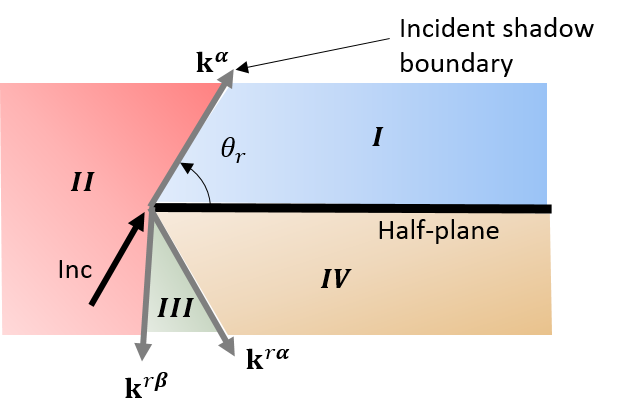
\includegraphics[height=0.33\textheight]{images/chapter1/ShadowBoundary.png}
    \caption{Incident wave on an edge}
    \label{illuzones}
\end{figure}

\subsection{\acrfull{gtd}}
The \acrfull{gtd} was initially developed by Keller \cite{GTD} for optical waves and adapted to elastodynamics by Achenbach and Gautesen \cite{AchenbachGautesen, Achenbach}. this theory postulates the existence of diffracted waves emanating from the edge of the scattering surface. A incident ray on an edge generates a cone of rays, called Keller's cone of diffraction \cite{GTD}, represented on Fig.~\ref{KellerCone}. The cone's principal axis is the diffracting edge, its principal angle is determined by Snell's law of diffraction :
\begin{equation}
    \frac{1}{c_{\alpha}}\cos\Omega_{\alpha} = \frac{1}{c_{\beta}} \cos\Omega_{\beta}
\end{equation}

\begin{figure}
    \centering
    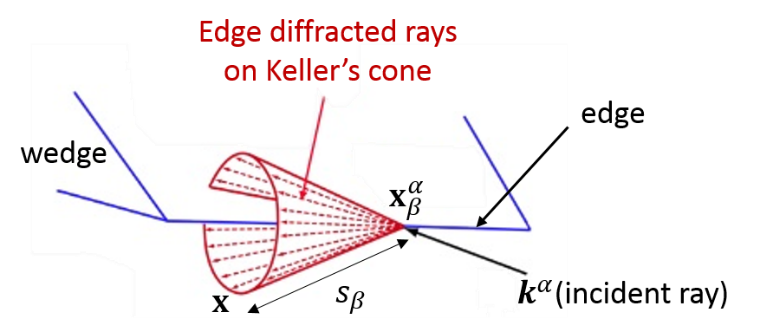
\includegraphics[width=\textwidth]{images/chapter1/KellerCone.png}
    \caption{Diffracted rays generated by an incident ray}
    \label{KellerCone}
\end{figure}

Rahmat-Samii \cite{ConePhoto} has observed this cone in a hotel room, see Fig.~\ref{PhotoCone}. A ray of light is incident on the corner of a table and generates a cone of diffracted rays, whose intersection with the door is a circle.

\begin{figure}
    \centering
    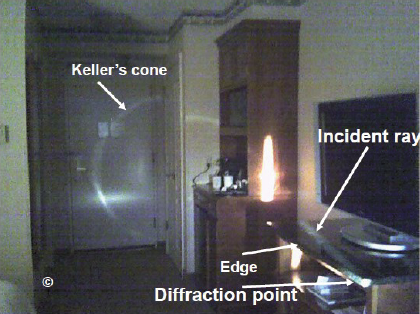
\includegraphics{images/chapter1/HotelCone.png}
    \caption{Observation of Keller's cone of diffraction}
    \label{PhotoCone}
\end{figure}

The \acrshort{gtd} is also a ray tracing method, meaning that at a given observation point $M$, the total field $\mathbf{u^{tot}}$ is the sum of the fields carried by each ray passing through $M$ :
\begin{equation}
    \mathbf{u^{tot}}(M)=\mathbf{u^{(GE)}}(M)+\sum_{\beta} \mathbf{u^{diff}_{\beta}}(M)
\end{equation}
where $u^{(GE)}$ is the \acrshort{ge} displacement field, composed of the incident, reflected and refracted fields and $u^{diff}_{\beta}$ is the diffracted field of type $\beta=L,TH,TV$. In this chapter, the bold font is used to denote vectors. The diffracted field's amplitude decreases as the distance $r$ from the point of impact $x_{\beta}^{\alpha}$ of the incident wave on the diffracting edge grows. As for the \acrshort{ge} field, the diffracted field is proportional to the field incident on the edge and this proportionality is characterized by a multiplicative coefficient called the diffraction coefficient, which depends on the propagation medium, on the geometry of the diffracting object and on the direction of observation. This is summarized by the following equation :
\begin{equation}
    \mathbf{u}_{\beta}^{diff}(M)=u_{\alpha}^{inc}(x_{\beta}^{\alpha})D_{\beta}^{\alpha}(M)\dfrac{e^{ik_{\beta}r}}{\sqrt{k_{\beta}R_{\beta}^{diff}}}\mathbf{e_{\beta}}(M)
\end{equation}
where $u_{\alpha}^{inc}$ is the value of the incident field, $D_{\beta}^{\alpha}$ is the diffraction coefficient, $k_{\beta}$ is the diffracted wave's wave number, $\mathbf{e_{\beta}}(M)$ is the unit polarisation vector of the diffracted wave at point M and $R_{\beta}^{diff}$ is a distance parameter which will be computed later, at section \ref{}.

This principle is called the locality principle, because it stipulates that the value of the field at any given point is fully determined by the field in the close vicinity of the point from which the ray carrying this field emanates. Computation of diffracted fields can therefore be reduced to a number of canonical problems, such as diffraction by a tip or a half plane. In the present thesis, the canonical problem of interest is diffraction by a wedge.

The \acrshort{gtd} is a high-frequency model which accounts for edge-diffracted waves. However, the resulting field is discontinuous at shadow boundaries and is therefore not physical. Some uniform corrections have been proposed to solve this problem, resulting in continuous fields. They are presented in the following. 

\section{Uniform corrections}
%% Maybe details only for UTD. Name PTD and UAT with principle behind it but not details (refer to litterature & AKD for these), give shortcomings and why need for UTD. Then briefly describe UTD. In each case, these are corrections of a GTD method -> need for good GTD

\subsection{\acrfull{ka}}
\subsection{\acrfull{ptd}}
\subsection{\acrfull{uat}}
\subsection{\acrfull{utd}}

\section{Existing \acrshort{gtd} models}
\subsection{The Sommerfeld Integral Method}
\subsection{The Laplace Transform Method}
%
% Deuxième chapitre

\chapter[][Acoustic Case]{The spectral functions method for acoustic wave diffraction by a stress-free
wedge : theory and validation}
\label{chap-developpement}


\section{Introduction}
The canonical problem of an acoustic, electromagnetic or elastodynamic plane wave diffraction by a wedge with Neumann or Dirichlet boundary conditions is a complex mathematical problem which has been of great interest to researchers for over a century.

The mathematical theory of wedge diffraction was first introduced by Sommerfeld \cite{Sommerfeld}, who gave an analytical expression of the exact solution of the diffraction problem of a scalar plane wave as a contour integral \cite{SMtechnique}. Macdonald \cite{Macdo} has expressed the scalar solution as a series, using the variables separation technique. Sommerfeld \cite{Sommerfeld} gave an analytical formula of the \acrfull{gtd} diffraction coefficient for an arbitrary-angled wedge (with Neumann or Dirichlet boundary conditions) illuminated by a scalar plane wave. This wedge \acrshort{gtd} coefficient can be used for scalar wave diffraction both in electromagnetics \cite{Kouyoumjian} and in acoustics \cite{Bouche,Bo}.

%In the more complex case of an elastic wave diffracted by a wedge of angle less than $\pi$, there exist two major approaches : one is based on the Sommerfeld integral (SI) representation of the elastodynamic potentials, it was introduced by Budaev and Bogy \cite{Rayleigh} and clarified by Kamotski et al. \cite{KamotskiFradkin}. The other method is based on the Laplace transform of the displacement field (LT), and was developed by Gautesen and Fradkin \cite{GautesenFradkin}. In the particular case of a scattered Rayleigh wave, a method which uses the free-space Green's tensor to express the Fourier transform of the displacement field has been developed by Gautesen for wedge angles smaller and greater than $\pi$ \cite{GautesenRayleigh,GautesenRayleigh2}. However the range of the wedge angle was restricted to the range $\lbrack 63^o,180^o\rbrack $ for angles smaller than $\pi$ and to $\lbrack 189^o,327^o \rbrack$ for angles greater than $\pi$ in order to avoid numerical instabilities.
%
%These methods are non-uniform in the sense that they lead to a solution which diverges at shadow boundaries and caustics of the Geometric-Elastic (GE) field \cite{Bouche}. To overcome this difficulty, Ufimtsev \cite{Ufmi} has introduced the Physical Theory of Diffraction (PTD) in electromagnetics. This technique has been extended to elastic waves by Zernov et al. \cite{Zernov}, however it is computationally expensive. 
%Another uniform correction of GTD is the Uniform Asymptotic Theory (UAT), introduced by Lewis \cite{Lewis} in electromagnetics and acoustics and extended to elastodynamics by Achenbach et al. \cite{Achenbach}, which gives a systematic approach for computing a uniform solution but is quite complicated to implement for complex geometries as it requires extension of the reflected field to its shadow zone using fictitious rays \cite{Bouche}, \cite{Molinet}.
%For practical purposes, the most used uniform correction of the GTD method is the Uniform Theory of Diffraction (UTD) as it is computationally efficient and does not require an artificial extension of the reflected field. It was developed in electromagnetics by Kouyoumjian and Pathak \cite{Kouyoumjian}, using the Pauli-Clemmow method \cite{Pauli} and extended to elastodynamics by Kamta Djakou et al. \cite{Audrey}. A comparison of different asymptotic (GTD and uniform) and exact solutions has been carried out in elastodynamics by Aristizabal et al. \cite{Aristizabal} but for the scalar case of the 2D wedge diffraction of a shear horizontally polarized incident wave.

%For a certain time, methods of computation have been studied without proof of solvability for the wedge diffraction problem. Osher \cite{Osher1, Osher2} has studied the well-posedness of hyperbolic initial and boundary value problems (meaning the solution is fixed at $t=0$ and on the domain boundaries) in a region with a corner (meaning a right-angled wedge) and has given certain necessary conditions that the boundary values must verify in order for a problem to be well-posed; he has thoroughly presented the consequences if these conditions were not verified. Huang and Temam \cite{Huang} have studied the well-posedness of hyperbolic initial and boundary value problems in a rectangular domain and have also specified how the boundary values must be chosen for the problem to be solvable; they have also given a brief explanation as to how their theory can be applied to wave equations.

These methods of computation have been proposed without proof of solvability for the wedge diffraction problem. Castro and Kapanadze \cite{Castro} have proven existence and uniqueness of the solution for acoustic and electromagnetic plane waves using a detailed Fredholm analysis. Kamotski and Lebeau \cite{KamotskiLebeau} have proven existence and uniqueness of the solution to the elastic plane wave diffraction  by a soft wedge (Dirichlet boundary) problem using the Spectral Functions method in which the diffracted wave is modeled thanks to these spectral functions. Their demonstration is valid for all wedge angles but they do not propose any method of computation of the solution. The Spectral Functions method was at first developed by Croisille and Lebeau \cite{CroisilleLebeau} who proposed a numerical algorithm in order to compute these functions for elastic wedges of angle lower than $\pi$ immersed in a fluid. In this chapter, wedges of any angle (even larger than $\pi$) are taken into account, and the outside medium is void. There is only one wave type to be considered and Dirichlet or Neumann boundary conditions are supposed, as opposed to the case studied by Croisille and Lebeau \cite{CroisilleLebeau} where three propagation modes coupled by the boundary conditions are considered, but only for wedge angles lower than $\pi$.

In the field of seismic diffraction, other approaches have been developed. The problem of acoustic diffraction in a system of wedge-shaped regions was studied by Klem-Musatov \cite{Klem-Musatov}. Using the Malyuzhinetz transform, this problem is reduced to a system of functional equations. However, this system is too complex to be solved in general cases. A successive approximations method is proposed in the particular case of a wedge-shaped separation between two media having the same acoustic wave velocity or  in the case where the medium containing the incident wave is a wedge of angle lower than $\pi$. In the very general case of acoustic wave propagation in a homogeneous or inhomogeneous medium delimited by an arbitrary-shaped boundary, a mathematical model has been rigorously presented by Aizenberg and Ayzenberg \cite{Aizenberg}, providing the analytical feasible fundamental solution for this problem. The notion of feasible fundamental solution is a generalization of Green's function for an unbounded medium. Ayzenberg \cite{Ayzenberg} shows how this general mathematical model can be numerically applied to the case of wedge diffraction. This method is applied in the case of a spherical source and it appears that parallel computation is necessary to obtain a short computation time, whereas the spectral functions method is applied here in the case of plane-wave diffraction and a simple architecture is sufficient to obtain results for a short computation time. 

The aim of this chapter is to develop and implement the methodology of Croisille and Lebeau \cite{CroisilleLebeau} in the two-dimensional (i.e. the incident wave vector lies in the plane normal to the edge) case of an acoustic wave diffracted by a soft wedge immersed in a fluid (Dirichlet boundary condition) and propose a numerical validation of the method for angles both smaller and larger than $\pi$.  The expansion to all wedge angles is obtained using Kamotski and Lebeau's \cite{KamotskiLebeau} idea of defining a new angular variable, $\widetilde{2\varphi}$, defined in equation \eqref{phitilde}, thanks to which the complete resolution and the computation of the solution are proposed and developed here for all wedge angles with a single method. Numerical validation will be achieved by comparing the GTD approximation of the diffraction coefficient obtained using the spectral functions method, with the analytical expression given in \cite{Bouche,Bo} of the GTD approximation of the exact solution. 

The outline of the chapter is the following: section \ref{Chapter5:problem}. presents the problem and the diffraction coefficients are expressed in terms of the spectral functions. The resolution of the problem is discussed in section \ref{Chapter5:resolution}. Finally, numerical results are given in section \ref{Chapter5:results}. and compared to the analytical Sommerfeld solution. 

\section{Problem statement}
\label{Chapter5:problem}

Let us consider a stress-free wedge of angle $\varphi$ immersed in a fluid $\Omega_f$ constituted of the junction of two faces $\mathcal{S}_1$ and $\mathcal{S}_2$ (see Fig.~\ref{chapter5:figure1}). The inward unit vectors normal to each of these faces are noted $n_1$ and $n_2$ respectively. The Cartesian coordinate system $(O; \mathbf{e}_{x_1}, \mathbf{e}_{y_1} )$ is linked to the face $\mathcal{S}_1$ of the wedge and $(O;  \mathbf{e}_{x_2}, \mathbf{e}_{y_2} )$ is linked to the face $\mathcal{S}_2$. These Cartesian coordinate systems  have the same origin located on the wedge edge which coincides with the $z$-axis. Let $\mathbf{x} = (x_1,y_1)_{ (\mathbf{e}_{x_1}, \mathbf{e}_{y_1}) } = (x_2,y_2)_{ (\mathbf{e}_{x_2}, \mathbf{e}_{y_2})}$ be a position vector $\mathbf{x} = (r,0)$ in a local basis of polar coordinates associated to the Cartesian coordinates $(x_1,y_1)$. The time convention used in this chapter is $\exp(i\omega t)$. The wedge is thus irradiated by a velocity potential plane wave in the form
\begin{align}
\label{Chapter5:incidence_wave}
g^{\rm inc}(\mathbf{x},t) = A \, e^{i(\omega t - \mathbf{k}^{\rm inc} \cdot \mathbf{x})}
\end{align}

where $A$ is the amplitude of the incident velocity potential, $\omega$ is the circular frequency, $t$ is time and 
\begin{align}
\mathbf{k}^{\rm inc} = k_0 (-\cos \theta_{\rm inc},-\sin \theta_{\rm inc})_{(\mathbf{e}_{x_1}, \mathbf{e}_{y_1})}
\end{align}
is the wave vector of the incident wave with $k_0 = \omega/c_0$ being the wave number and $c_0$ is the sound velocity in the fluid.  The velocity potential in the fluid $g$ satisfies the motion equation in the fluid medium $\Omega_f$ surrounding the wedge 
\begin{equation}
\label{Chapter5:WaveMotion}
\frac{\partial^2 g}{\partial t^2} - c_0^2 \, \triangle g = 0
\end{equation}
and the boundary condition on the wedges faces
\begin{equation}
\label{Chapter5:CL}
Bg\mid_{\mathcal{S}_j} = 0, \quad j=1,2,
\end{equation}
where the expression of operator B is given by \eqref{Chapter5:CLDir} for Dirichlet boundary conditions and by \eqref{Chapter5:CLNeu} for Neumann boundary conditoins :
\begin{subequations}
\begin{equation}
\label{Chapter5:CLDir}
Bg = g \quad \mbox{for Dirichlet boundary conditons}
\end{equation}
\begin{equation}
\label{Chapter5:CLNeu}
Bg = \frac{\partial g}{\partial n} \quad \mbox{for Neumann boundary conditons}
\end{equation}
\end{subequations}

This common notation makes it possible to treat both cases simultaneously in the following developments.

\begin{figure}[h]
\centering
	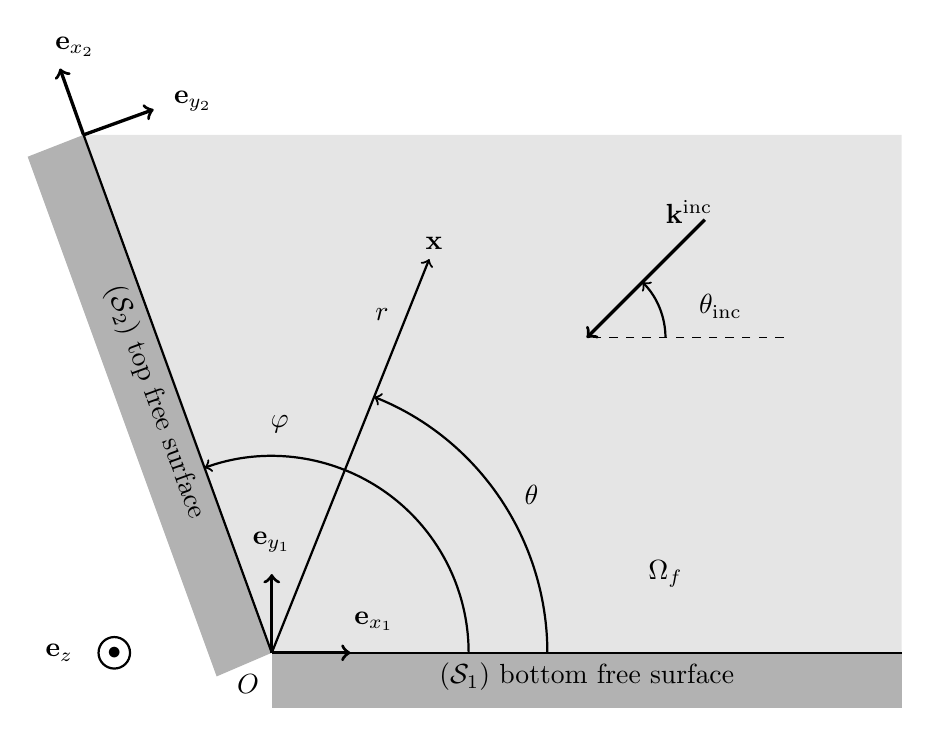
\begin{tikzpicture}
	\fill[color=gray!20] (0,0) -- (8,0)  -- (8,6.5778) -- (-2.39,6.5778) -- cycle;  
	\draw[ thick, ->] (2.5,0) arc (0:110:2.5);
	
	\fill[color=gray!60] (0,0) -- (8,0)  -- (8,-0.7) -- (0,-0.7) -- cycle;  
	
	\fill[color=gray!60] (0,0) --  (-2.39,6.5778) --(-3.1,6.3) -- (-0.7,-0.3) -- cycle; 
		
	\draw[thick, color = black]  (0,0) -- (8,0) node[midway,below] {($\mathcal{S}_1$) bottom free surface};
	
	\draw[thick, color = black]  (0,0) -- (-2.39,6.5778) node[midway,below,sloped] {($\mathcal{S}_2$) top free surface};
	
	\draw[very thick, ->] (-2.39,6.5778) -- (-2.69,7.42);
	
	\node[scale=1] at (-2.5,7.7){$\mathbf{e}_{x_2}$};
	
	\draw[very thick, ->] (-2.39,6.5778) -- (-1.5,6.9);
	
	\node at (-1,7){$\mathbf{e}_{y_2} $};
	
	
	\node at (0.1,2.9){$\varphi$} ; 
	
	\draw[very thick, ->] (0,0) -- (1,0);
	
	\node at (1.3,0.4) {$\mathbf{e}_{x_1} $};
	
	\draw[very thick, ->] (0,0) -- (0,1);
	
	\node at (0,1.4){$\mathbf{e}_{y_1} $};
	
	\node at (-2,-0.01) {$\bullet$};
	
	\draw[thick] (-2,0) circle (0.2);
	
	\node at (-2.7,0){$\mathbf{e}_{z}$};
	
	\draw[very thick, ->] (5.5,5.5) -- (4,4);
	
	\draw[dashed] (6.5,4) -- (4,4);
	
	\draw[thick, ->] (5,4) arc (0:45:1);
	
	\node at (5.7,4.4){$\theta_{\rm inc}$};
	
	\node at (5.3,5.6){ $\mathbf{k}^{\rm inc}$};
	
	\node at (-0.3,-0.4){ $O$};
	
	\node at (5,1){$\Omega_f$ };
	
	% point observation
	
	\draw[thick, ->] (0,0) -- (2,5); 
	
	\draw[thick, ->] (3.5,0) arc (0:68.2:3.5);
	
	\node at (3.3,2){$\theta$};
	
	\node at (1.4,4.3){$r$};
	
	\node at (2.06,5.2){$\mathbf{x}$};
	
	\end{tikzpicture}
	\caption
[Geometry of the problem]
{The wedge of angle $2\varphi$ whose faces are stress-free is illuminated by a plane wave of wave vector $\mathbf{k}^{\rm inc}$.}
\label{chapter5:figure1}
\end{figure}
The dimensionless form of the problem is obtained  by defining the function $h$ by
\begin{equation}
\label{Chapter5:dimensionless}
g(\mathbf{x},t) = 2A \, e^{i \omega t} \, h(k_0 \mathbf{x}).  
\end{equation}

The dimensionless function $h$ is the sum of the  incident dimensionless  wave $h_{inc}$ and of the scattered dimensionless  wave $v$
\begin{equation}
h = h_{inc} + v
\label{decompinc}
\end{equation}
In this decomposition, the scattered wave $v$ is the sum of two fields : the Geometric-Elastodynamic (GE) field, which  is the sum of the possibly multiple specular reflections of the incident wave and of fictitious fields compensating the incident wave in shadow zones, and the diffracted field. A detailed description of the GE field, in the case of a half-plane scatterer, is given by Kamta-Djakou et al. \cite{Audrey}.

The system \eqref{Chapter5:WaveMotion}-\eqref{Chapter5:CL} is equivalent to the following  system of equations for the dimensionless problem, obtained by inserting Fourier transform \eqref{Chapter5:dimensionless} and decomposition \eqref{decompinc} into equations \eqref{Chapter5:WaveMotion} and \eqref{Chapter5:CL}
\begin{equation}
\label{Chapter5:Adimen_waveMotion}
\begin{cases}
(\triangle+1)v =  0 \quad \text{in } \Omega_f, \\
Bv =  -Bh_{inc} \quad \quad \quad \text{on } \mathcal{S}_j, \quad j=1,2
\end{cases}.
\end{equation}

In order to obtain a solution to this problem which is physically relevant, the limiting absorption principle is used. It consists in substituting the wave number $k_0$ by a complex one $k_0 e^{-i\epsilon} $ with $\epsilon > 0$. This means that absorption occurs in the medium and thus the scattered waves attenuate with the distance. The system (\ref{Chapter5:Adimen_waveMotion}) then becomes :
\begin{equation}
\label{Chapter5:waveMotion_epsilon}
(S_\epsilon^*) \quad
\begin{cases}
(\triangle+ \, e^{-2i\epsilon}) v^\epsilon  =  0 \quad \text{in } \Omega_f, \\
Bv^\epsilon  =  -Bh_{\rm inc}^\epsilon  \quad \text{on } \mathcal{S}_j, \quad j=1,2
\end{cases}
\end{equation}

The physically relevant solution to (\ref{Chapter5:Adimen_waveMotion}), called the outgoing solution, can now be defined. It is the one obtained when taking $\epsilon \to 0$ in (\ref{Chapter5:waveMotion_epsilon}). This limit is noted $v^0$. Its integral representation is found hereafter.

\subsection*{Outgoing solution: integral representation}
\label{integral_representation}

First, a special class of distributions is defined.
\begin{definition}
The class of distributions $\mathcal{A}$ is defined as follows. The distribution $f\in \mathcal{A}$ if :
\begin{itemize}
\item $f \in \mathcal{L}^2(\mathbb{R})$ (f is a tempered distribution)
\item supp$(f) \subset \lbrack 0,+\infty \lbrack$
\item $\exists C_0>0$ such that
$$ \sup_{-\pi<\theta<0} \int_{\rho>C_0}|\hat{f}(\rho e^{i\theta})|^2\,d\rho <\infty$$
where $\hat{f}$ is the Fourier transform of $f$ defined by $\hat{f}(\xi)=\int_{\mathbb{R}}f(x)e^{-ix\xi}\, dx$.
\item $\hat{f}(\xi)$ is holomorphic near $\xi=1$
\end{itemize}

\end{definition}
The outgoing solution to (\ref{Chapter5:Adimen_waveMotion}) can now be defined properly.

\begin{definition}
An outgoing solution of the equation (\ref{Chapter5:Adimen_waveMotion}) is a solution v of the form 
\begin{equation}
\label{Chapter5:decomposition}
v=v_1|_{\Omega_f}+v_2|_{\Omega_f}
\end{equation}
where, for $j=1,2$ :
\begin{equation}
\label{inv_potentiels}
v_j=-\lim_{\epsilon \to 0} \left(\Delta+e^{-2i\epsilon}\right)^{-1} \left[ \alpha_j \otimes \delta_{\mathcal{S}_j} \right]
\end{equation}
$\alpha_j \in \mathcal{A}$ are unknown and $\delta_{\mathcal{S}_1}$ and $\delta_{\mathcal{S}_2}$ are the Dirac delta functions on the faces $\mathcal{S}_1$ and $\mathcal{S}_2$ of the wedge respectively (these functions verify $\delta_{\mathcal{S}_j}(x,y)=1$ on $\mathcal{S}_j$, and $\delta_{\mathcal{S}_j}(x,y)=0$ elsewhere).

\end{definition}
The following theorem is proven by Croisille and Lebeau in \cite{CroisilleLebeau} :
\begin{theorem}
The equation \eqref{Chapter5:Adimen_waveMotion} admits a unique outgoing solution.
\end{theorem}

The aim of this chapter is to extend and detail the computation of this outgoing solution for the stress-free wedge immersed in a fluid using the spectral functions method.

The double Fourier transform of a tempered distribution and its inverse are defined by :
\begin{subequations}
\begin{equation}
\hat{f}(\xi,\eta)=\int \int_{\mathbb{R}^2}f(x,y)e^{-i(x\xi+y\eta)}\, {\rm d}x {\rm d}y
\label{fourierdef}
\end{equation}
\begin{equation}
f(x,y)=\frac{1}{4\pi^2}\int\int_{\mathbb{R}^2} \hat{f}(\xi,\eta)e^{i(x\xi+y\eta)}\rm d\xi \rm d\eta
\label{invfourierdef}
\end{equation}
\label{fullfourierdef}
\end{subequations}

The double Fourier transform of (\ref{inv_potentiels}) using \eqref{fourierdef} gives
\begin{equation}
\label{Fourier}
\hat{v_j^\epsilon} =  \left[ \xi^2 + \eta^2 - e^{-2i\epsilon} \right]^{-1} \hat{\alpha_j}.
\end{equation}

 The dimensionless velocity potential $v_j^\epsilon$ is then found by applying the inverse Fourier transform in $\xi$ and $\eta$ to \eqref{Fourier}. 
\begin{equation}
\label{velocity_inv_fourier2}
v_j^\epsilon = \dfrac{1}{4\pi^2}  \int_{-\infty}^{+\infty}\left( \int_{-\infty}^{+\infty} \dfrac{e^{iy_j\eta}}{ \xi^2 + \eta^2 - e^{-2i\epsilon}} {\rm d}\eta \right)\,  \hat{\alpha_j}(\xi) \,  e^{i x_j \xi}  {\rm d} \xi.
\end{equation}

For  $\epsilon \neq 0$, the inner integrand poles are given by
\begin{equation}
 \eta = \pm \sqrt{e^{-2i\epsilon} - \xi^2}  = \pm \zeta_0^\epsilon
\end{equation} 
and are never crossed by integration along the real axis. Integral \eqref{velocity_inv_fourier2} can be calculated using the residue theorem which leads to the following result
\begin{equation}
\label{champ_epsilon}
v_j^\epsilon(x_j,y_j) = \dfrac{i}{4\pi} \int_{-\infty}^{+\infty}  \dfrac{e^{i|y_j|\zeta_0^\epsilon(\xi)} e^{i x_j \xi}}{\zeta_0^\epsilon(\xi)} \hat{\alpha_j}(\xi) \, {\rm d}\xi.
\end{equation}
This integral is well defined if $\text{Im}(\zeta_0^\epsilon) > 0$, so that the exponential in the integral decreases with the distance $y_j$ and the absorption principle is respected. Function $\zeta_0^\epsilon(\xi)$ then satisfies for $\xi$ real
\begin{subequations}
\label{zeta_function}
\begin{align}
\zeta_0^\epsilon(\xi)&= i\sqrt{\xi^2-e^{-i\epsilon}} \quad \text{if} \quad \vert \xi\vert \geq 1,\\
\label{zeta_function_inferior1}
\zeta_0^\epsilon(\xi)&= -\sqrt{e^{-i\epsilon}-\xi^2} \quad  \text{if} \quad \vert \xi\vert \leq 1.
\end{align}
\end{subequations}
The branch points of the function $\zeta_0^\epsilon(\xi)$ are $\pm  \, e^{-i\epsilon}$. For $\epsilon > 0$, integral \eqref{champ_epsilon} is well defined because these complex singular points are never crossed by the integration contour (the real axis). The integration contour of \eqref{champ_epsilon}, is deformed into the contour $\Gamma_0$ illustrated on Fig.~\ref{chapter5:figure2} so that these singular points $\pm  \, e^{-i\epsilon}$ are not crossed by the new contour $\Gamma_0$  when $\epsilon \rightarrow 0$ (for which the physical outgoing solution of (\ref{Chapter5:waveMotion_epsilon}) is obtained). The curved arrows on Fig.~\ref{chapter5:figure2} are described later in section \ref{Chapter5:regular_part}.

Thus, even for $\epsilon=0$, the integral
\begin{equation}
\label{champ}
v_j^0(x_j,y_j) = \dfrac{i}{4\pi} \int_{\Gamma_0}  \dfrac{e^{i|y_j|\zeta_0^0(\xi)} e^{i x_j \xi}}{\zeta_0^0(\xi)} \hat{\alpha_j}(\xi)  \, {\rm d}\xi
\end{equation}
converges.
Using \eqref{Chapter5:decomposition}, our initial solution is then
\begin{equation}
\label{initial_sol}
v(\mathbf{x}) = v_1^0(x_1,y_1) + v_2^0(x_2,y_2)
\end{equation}

\begin{figure}[ht]%
	\centering
	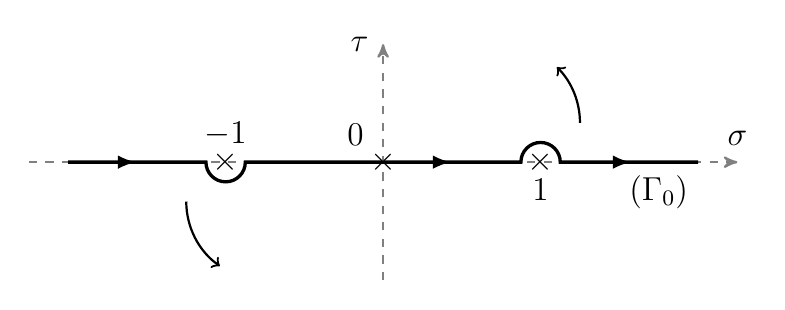
\begin{tikzpicture}
	\node at (0,0) {\large $\times$};
	\node at (-0.35,0.35) {\large $0$};
	\node at (2,0) {\large $\times$}; % Pole
	\node at (2,-0.35) {\large $1$};
	\node at (-2,0) {\large $\times$};
	\node at (-2,0.35) {\large $-1$}; %pole
	\node at (3.5,-0.38) {\large $(\Gamma_0)$};
	\draw[ thick, ->] (-2.5,-0.5) arc (180:235:1);
%	\node at (-2.8,-0.9) {\large $\mathcal{F}_1$};
	\draw[ thick, ->] (2.5,0.5) arc (0:45:1); %ici c'est les fleches 
	%\node at (2.8,0.9) {\large $\mathcal{F}_2$};
    \node at (4.5,0.3) {\large $\sigma$};
    \node at (-0.3,1.5) {\large $\tau$};
	\draw[step=1.5cm,gray,thick,dashed,->,>=stealth'] (-4.5,0) -- (4.5,0);
	\draw[step=1.5cm,gray,thick,dashed,->,>=stealth'] (0,-1.5) -- (0,1.5);
	\draw[very thick,black,yshift=0pt,
	decoration={ markings,  % This schema allows for fine-tuning the positions of arrows 
		mark=at position 0.1 with {\arrow{latex}},
		mark=at position 0.6 with {\arrow{latex}},
		mark=at position 0.9 with {\arrow{latex}}},
	postaction={decorate}]
	(-4,0)  -- (-2.25,0)  arc (-180:0:0.25)  -- (1.75,0)arc (180:0:0.25)  --  (4,0); % ca c'est l'axe
	\end{tikzpicture}
\caption
[Contour $\Gamma_0$]
{Integration contour $\Gamma_0$ in the complex plane $\xi = \sigma + i \tau$. The curved arrows show the deformation of $\Gamma_0$ into the imaginary axis.}
\label{chapter5:figure2}
\end{figure}

One of the goals of this chapter is to compute the spectral functions $\hat{\alpha}_1(\xi)$ and $\hat{\alpha}_2(\xi)$ in order to find the GTD diffraction coefficient \eqref{GTDCoeff_SF}. The accuracy of the spectral functions method is evaluated in section 4 by comparing results of \eqref{GTDCoeff_SF} with \eqref{GTDCoeff_Dir} in the case of Dirichlet boundary conditions and \eqref{GTDCoeff_Neu} in the case of Neumann boundary conditions. Section \ref{Chapter5:resolution} is devoted to the computation of the spectral functions $\hat{\alpha}_1$ and $\hat{\alpha}_2$.


\section{Spectral functions computation}
\label{Chapter5:resolution}

To compute the spectral functions, the functional equations satisfied by these spectral functions $\hat{\alpha}_1$ and $\hat{\alpha}_2$ first have to be determined.
\subsection{Functional equations of spectral functions}

The velocity potential in the boundary conditions of the system \eqref{Chapter5:waveMotion_epsilon} is substituted by its expression \eqref{initial_sol}. It then leads to the following system of equations for the boundary conditions on each wedge face:
\begin{equation}
\label{CL}
\begin{cases}
Bv_1^0(x_1,0) + Bv_2^0(x_2 \cos \varphi,x_2 \sin \varphi)  =  -Bv^0_{\rm inc} \mid_{\mathcal{S}_1}\\
Bv_1^0(x_1 \cos \varphi,x_1 \sin \varphi) + Bv_2^0(x_2,0)   =  -Bv^0_{\rm inc} \mid_{\mathcal{S}_2}
\end{cases}.
\end{equation}
The Fourier transform is applied to the potential velocity expression on the face of each wedge
\begin{align}
\mathcal{F}(x_j \mapsto v_j^0 (x_j,0))(\xi) & =  \dfrac{i}{4\pi} \int_{\Gamma_0}  \dfrac{\hat{\alpha_j}(\lambda)}{\zeta_0^0(\lambda)}  \left( \int_0^{\infty} \, e^{-i x_j (\xi-\lambda)} dx_j \right) {\rm d} \lambda,\\
& =  \dfrac{1}{4\pi} \int_{\Gamma_0} \dfrac{\hat{\alpha_j}(\lambda)}{\zeta_0^0(\lambda) (\xi - \lambda)} {\rm d} \lambda \nonumber
\end{align}
and
\begin{align}
\mathcal{F} \left( x_j \mapsto v_j^0 \left( x_j \cos \varphi,x_j \sin \varphi \right) \right)(\xi)  & =  \dfrac{i}{4\pi} \int_{\Gamma_0}  \dfrac{\hat{\alpha_j}(\lambda)}{\zeta_0^0(\lambda)}  \left( \int_0^{\infty} \, e^{-i x_j \left( \xi - \lambda  \, \cos \varphi - |\sin \varphi| \, \zeta_0^0(\lambda) \right)} dx_j \right) {\rm d} \lambda,\\
& = \dfrac{1}{4\pi} \int_{\Gamma_0} \dfrac{ \hat{\alpha_j}(\lambda)}{\zeta_0^0(\lambda) \left[ \xi - \lambda \, \cos \varphi  - |\sin \varphi| \, \zeta_0^0(\lambda) \right]} {\rm d} \lambda.  \nonumber
\end{align}
The potential velocity's normal derivative on the face of each wedge is computed using \eqref{champ}, and by noting that for each face $n_j=y_j$ (see Fig.~\ref{chapter5:figure1}) :
\begin{equation}
\frac{\partial v_j^0}{\partial n_j}(x_j,y_j) = -\frac{1}{4\pi} \int_{\Gamma_0} te^{i\xi x_j}e^{i|y_j|\zeta_0^0(\xi)} \hat{\alpha_j}(\xi)\, d\xi,
\end{equation}
where $t= \rm sgn \, y_j$. In order to go from one Cartesian coordinate system to another, the following change in variables is given for $j=1,2$ (see Fig.~\ref{chapter5:figure1}) :
\begin{eqnarray}
\label{changecoords}
\left\{
\begin{array}{l}
x_{3-j}=x_j\cos\varphi+y_j\sin\varphi \\
y_{3-j}=x_j\sin\varphi-y_j\cos\varphi
\end{array}
\right.
\end{eqnarray}
This yields :
\begin{align}
\frac{\partial v_j^0}{\partial n_{3-j}}&=\frac{\partial v_j^0}{\partial y_{3-j}}= \sin\varphi \frac{\partial v_j^0}{\partial x_j}-\cos\varphi \frac{\partial v_j^0}{\partial y_j}\\
&=-\frac{1}{4\pi}\int_{\Gamma_0}\frac{(\xi\sin\varphi-t\cos\varphi\zeta_0^0(\xi))}{\zeta_0^0(\xi)}e^{i(\xi x_j+|y_j|\zeta_0^0(\xi))}\hat{\alpha_j}(\xi)\,d\xi
\end{align}
The Fourier transform can now also be applied to the potential velocity's normal derivative on the each face of the wedge
\begin{align}
\mathcal{F}(x_j \mapsto \frac{\partial v_j^0}{\partial n_j} (x_j,0))(\xi)&=-\frac{1}{4\pi} \int_{\Gamma_0}  \hat{\alpha_j}(\lambda)\left( \int_0^{\infty} \, e^{-i x_j (\xi-\lambda)} dx_j \right)\, d \lambda \nonumber\\
&=\frac{i}{4\pi}\int_{\Gamma_0}\frac{\hat{\alpha_j}}{\xi-\lambda}\, d\lambda
\end{align}
and
\begin{align}
\mathcal{F} &\left( x_j \mapsto \frac{\partial v_j^0}{\partial n_{3-j}} ( x_j \cos \varphi,x_j \sin \varphi) \right)(\xi)  \nonumber\\
& =  -\frac{1}{4\pi} \int_{\Gamma_0}  \frac{(\lambda\sin\varphi-t\cos\varphi\zeta_0^0(\lambda))}{\zeta_0^0(\lambda)}\hat{\alpha_j}(\lambda)  \left( \int_0^{\infty} \, e^{-i x_j \left( \xi - \lambda  \, \cos \varphi - |\sin \varphi| \, \zeta_0^0(\lambda) \right)} dx_j \right) \,d \lambda, \nonumber\\
& = \frac{i}{4\pi} \int_{\Gamma_0} \dfrac{ \lbrack \lambda\sin\varphi-t\cos\varphi\zeta_0^0(\lambda)\rbrack \, \hat{\alpha_j}(\lambda)}{\zeta_0^0(\lambda) \left[ \xi - \lambda \, \cos \varphi  - |\sin \varphi| \, \zeta_0^0(\lambda) \right]} \, d\lambda,
\end{align}
here $t=\rm sgn \sin \varphi$.

The dimensionless incident wave on the faces $\mathcal{S}_1$ and $\mathcal{S}_2$ of the wedge which is involved at the right side of \eqref{CL} is respectively:
\begin{subequations}
\label{CL2}
\begin{align}
v^0_{\rm inc}(x_1,y_1) & =  \dfrac{1}{2} \, e^{i \, (x_1 \cos \theta_{inc}+y_1\sin\theta_{inc} ) } ,\\
v^0_{\rm inc}(x_2,y_2) & =   \dfrac{1}{2} \, e^{i \, (x_2 \cos (\varphi - \theta_{inc} )+y_2\sin(\varphi-\theta_{inc}))} 
\end{align}
\end{subequations}

Therefore, applying the Fourier transform to \eqref{CL} leads to the following functional system of equations:
\begin{equation}
\label{functional_eq}
\begin{cases}
DM(\hat{\alpha}_1)(\xi) + TM(\hat{\alpha}_2)(\xi) = \dfrac{W_1}{\xi - Z_1} \\
TM(\hat{\alpha}_1)(\xi) + DM(\hat{\alpha}_2)(\xi)  = \dfrac{W_2}{\xi - Z_2} 
\end{cases}
\end{equation}
where $Z_1 =  \cos \theta_{\rm inc}$, $Z_2 =  \cos (\varphi - \theta_{\rm inc})$, $W_1=W_2=1$ in the case of Dirichlet boundary conditions and $W_1=\sin\theta_{inc}, \quad W_2=\sin(\varphi-\theta_{inc})$ in the case of Neumann boundary conditions. $DM$ is an integral operator defined as
\begin{equation}
\label{DM_operator}
\begin{split}
DM(\hat{\alpha}_1)(\xi) = \int_{\Gamma_0} DM(\xi,\lambda) \, \hat{\alpha}_1(\lambda) \, d \lambda =\dfrac{1}{2i\pi} \int_{\Gamma_0} \dfrac{dm(\lambda)  }{\xi - \lambda} \hat{\alpha}_1(\lambda) \, d\lambda
\end{split}
\end{equation}
where 
\begin{equation}
\label{dmDir}
dm(\lambda) = \dfrac{1}{\zeta_0^0(\lambda)}
\end{equation}
in the case of Dirichlet boundary conditions and 
\begin{equation}
\label{dmNeu}
dm(\lambda)=1
\end{equation}
in the case of Neumann boundary conditions. 

$TM$ is an integral operator defined as
\begin{equation}
\label{TM_operator}
\begin{split}
TM(\hat{\alpha}_1)(\xi) &= \int_{\Gamma_0} TM(\xi,\lambda) \, \hat{\alpha}_1(\lambda) \, {\rm d} \lambda =\dfrac{1}{2i\pi} \int_{\Gamma_0} \dfrac{ tm(\lambda)}{ \xi- \lambda \cos \varphi  - |\sin \varphi| \zeta_0^0(\lambda)} \hat{\alpha}_1(\lambda) \, {\rm d} \lambda 
\end{split}
\end{equation}
where 
\begin{equation}
\label{tmDir}
tm(\lambda)=\dfrac{1}{\zeta_0^0(\lambda)}
\end{equation}
in the case of Dirichlet boundary conditions and 
\begin{equation}
\label{tmNeu}
tm(\lambda)=\dfrac{\lambda\sin\varphi-t\cos\varphi\zeta_0^0(\lambda)}{\zeta_0^0(\lambda)}
\end{equation}
in the case of Neumann boundary conditions.
Note that the function $TM$ can be expressed as
\begin{equation}
TM(\xi,\lambda) =  \dfrac{1}{2i\pi} \dfrac{ tm(\lambda)}{ \xi- T_0(\lambda)} , 
\end{equation}
where, applying the variable change $\lambda=\cos\theta$
\begin{equation}
\label{Trans_operator}
T_0(\lambda=\cos\theta) =  \lambda \cos \phiti  + \sin \phiti \, \zeta_0^0(\lambda) =  \cos (\theta + \phiti)
\end{equation}
with 
\begin{equation}
\phiti =
\begin{cases}
 \varphi \quad \text{if} \quad 0 < \varphi < \pi \qquad \\
 2\pi - \varphi \quad \text{if} \quad \pi < \varphi < 2\pi
 \label{phitilde}
\end{cases}
\end{equation}
Function $T_0$ is therefore called the translation operator, since it translates the complex angle $\theta$ to $\theta+\phiti$. By using this angular variable, defined differently for wedge angles lower and higher than $\pi$, the description of the spectral functions method can be written the same way for wedge angles lower and higher than $\pi$, even if the final results (the diffraction coefficients) are different for wedge angles $\pi<\varphi<2\pi$ and $2\pi-\varphi$. Indeed, the variable $\varphi$ appears in all the resolution, whereas the variable $\phiti$ appears only in the definition of the function $T_0$ in \eqref{Trans_operator} and of the domain $\Omega_0$ in which $T_0$ operates, defined as
\begin{equation}
\label{Domain_Omega0}
\Omega_0 =\{\xi\in\mathbb C, \ \xi=\cos \theta, \ 0< {\rm Re } \, \theta < \pi -\phiti \}.
\end{equation}
Domain $\Omega_0$ is delineated by the hyperbola 
\begin{equation}
\partial \Omega_0^+ = \{   \xi \in \mathbb{C}, \quad \xi = \cos \theta, \quad {\rm Re}  \theta = \pi - \phiti \}.
\end{equation}
Domain $\Omega_0$ and its upper boundary $\partial \Omega_0^+$ are illustrated on Fig.~\ref{chapter5:figure4}. Domain $\Omega_0$ is the grey area in Fig.~\ref{chapter5:figure4}.

\begin{figure}[h]
\centering
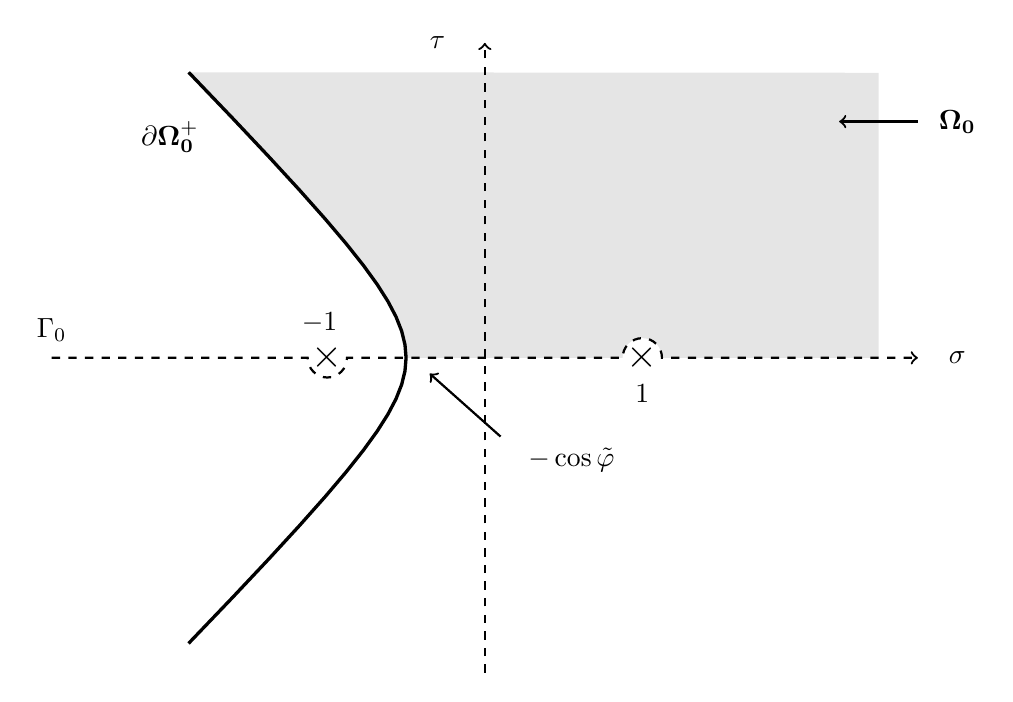
\begin{tikzpicture}
% Filling Omega_0
\fill [color=gray!20]
(5,0)
-- plot [domain=0:2] ({-cosh(\x)},{sinh(\x)})
-- (5,3.62)
-- cycle;

\fill[color=white] (2,0) circle (0.25);

\node at (2,0) {\Large $\mathbf{\times}$}; % Pole
\node at (2,-0.45) { $1$};
\node at (-2,0) {\Large $\mathbf{\times}$};
\node at (-2.1,0.45) {$-1$}; %pole
\node at (-5.5,0.35) {$\Gamma_0$};
\draw[dashed,thick, ->]
      (-5.5,0) -- (-2.25,0)  arc (-180:0:0.25)  -- (1.75,0)arc (180:0:0.25) -- (5.5,0);
\draw[dashed,thick,->]
	  (0,-4) -- (0,4);
\node at (6,0) {$\sigma$};
\node at (-0.6,4) { $\tau$};
      % axis

%% arrows indicating countour deformation
%\draw[ thick, ->] (-3,-0.25) arc (180:235:1);
%\node at (-3.2,-0.9) {$\mathcal{F}_1$};
%\draw[ thick, ->] (4.0,0.3) arc (0:45:1); 
%\node at (4.5,0.8) { $\mathcal{F}_2$};

% Hyperbola (contour  partial_Omega_0 )
\draw[black, very thick][domain=-2:2] plot({-cosh(\x)}, {sinh(\x)});
\node at (-4.0,2.8) { $\mathbf{\partial \Omega_0^+}$};
\draw[thick,->] (0.2,-1.0)--(-0.7,-0.2);
\node at (1.1,-1.3) {$-\cos \phiti$};

%  Omega_0
\draw [thick, ->] (5.5,3)--(4.5,3);
\node at (6,3) {$\mathbf{\Omega_0}$};

\end{tikzpicture}
\caption
[Contour $\partial \Omega_0^+$]
{Domain $\Omega_0$ (the grey area) and its upper boundary $\partial \Omega_0^+$. The lower boundary of $\Omega_0$ is the semi-axis $[-\cos \phiti,+\infty[$.}
\label{chapter5:figure4}
\end{figure}
Having found the system of functional equations, it is now resolved following the methodology of Croisille and Lebeau \cite{CroisilleLebeau}.

\subsection{System resolution}
\label{Chapter5:System_resolution}

The resolution of the system of functional equations \eqref{functional_eq} is necessary in order to find the values of the spectral functions $\hat{\alpha}_1 $ and $\hat{\alpha}_2 $. With these values, the diffraction coefficients can be computed using equation \eqref{GTDCoeff_SF}. 

It is shown in \cite{CroisilleLebeau} that $DM$ and $TM$ integral operators are constituted of a "singular term" and of a "regular term". For a singular function 
\begin{equation}
\label{Chapter5:arbitrary_function}
\phi(\xi) = \dfrac{1}{\xi - z},  \quad z \in \mathbb{C}\setminus ]-\infty,-1] \text{ with } {\rm Im} \, z \geqslant 0,
\end{equation}
$DM$ and $TM$ integral operators defined respectively in \eqref{DM_operator} and \eqref{TM_operator} can be decomposed using the residue theorem as
\begin{subequations}
\label{Int_op_decomp}
\begin{align}
\label{Int_op_decomp_DM}
DM(\phi)(\xi) &= \int_{\Gamma_0} DM(\xi,\lambda) \cdot \dfrac{1}{\lambda - z} \, d \lambda = \dfrac{dm(z)}{\xi - z}  + D_p(\xi,z) \\
\label{Int_op_decomp_TM}
TM(\phi)(\xi) &= \int_{\Gamma_0} TM(\xi,\lambda) \cdot \dfrac{1}{\lambda - z} \, d \lambda = \dfrac{tm(z) }{\xi - T_0(z)} 1_{\Omega_0}(z) + T_p(\xi,z),
\end{align}
\end{subequations}
where the function $T_0$ is defined in \eqref{Trans_operator} and where
\begin{equation}
1_{\Omega_0}(z) = 
\begin{cases}
1 \quad \text{if } z  \in \Omega_0, \\
0 \quad \text{else}
\end{cases}
\end{equation}
and integrals $D_p$ and $T_p$ are holomorphic on $\mathbb{C}\setminus ]-\infty,-1]$. Such integrals are expressed as
\begin{subequations}
\label{holomorphic_functions}
\begin{align}
\label{defDp}
D_p(\xi,z) &= \dfrac{1}{2\pi i}\int_{\Gamma_1} \dfrac{dm(\lambda)}{\xi-\lambda} \cdot \dfrac{1}{\lambda - z} d\lambda, \\
\label{defTp}
T_p(\xi,z) &= \dfrac{1}{2\pi i}\int_{\partial \Omega_0^+}  \dfrac{tm(\lambda)}{\xi-T_0(\lambda)} \cdot \dfrac{1}{\lambda - z} d\lambda.
\end{align}
\end{subequations}
Contours $\Gamma_1$ and $\partial \Omega_0^+$ are illustrated on Figs.~\ref{chapter5:figure5} and \ref{chapter5:figure4} respectively.

\begin{figure}[ht]
\centering
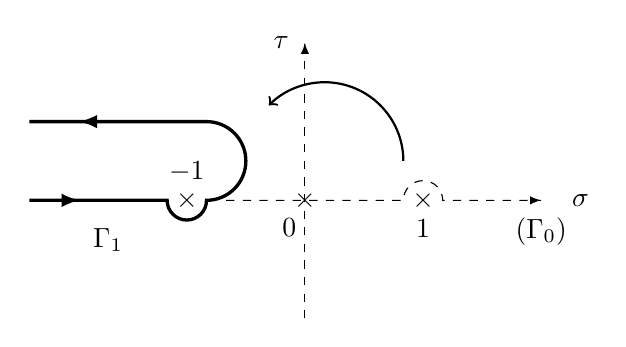
\begin{tikzpicture}
\node at (-0.5,0) {  $\times$};
\node at (-0.7,-0.35) { $0$};
\node at (1,0) { $\times$}; % Pole
\node at (1,-0.36) { $1$};

\node at (-2,0) { $\times$};
\node at (-2,0.36) {  $-1$}; %pole
\node at (-3,-0.5) { $\Gamma_1$};

\draw[dashed, decoration={markings,
 mark=at position 1.0 with {\arrow{latex}}},
      postaction={decorate}] (-1.5,0) -- (0.75,0) arc (180:0:0.25)-- (2.5,0);
\node at (3,0) {$\sigma$};
\draw[dashed, decoration={markings,
 mark=at position 1.0 with {\arrow{latex}}},
      postaction={decorate}] (-0.5,-1.5) -- (-0.5,2);
\node at (-0.8,2) {$\tau$};      

\node at (2.5,-0.4) {$(\Gamma_0)$};
      
\draw[ thick, ->] (0.75,0.5) arc (0:135:1); 
  

\draw[very thick, black, yshift=0pt,
decoration={ markings,  % This schema allows for fine-tuning the positions of arrows 
      mark=at position 0.1 with {\arrow{latex}},
      mark=at position 0.9 with {\arrow{latex}}},
      postaction={decorate}]
      (-4,0) -- (-2.25,0)  arc (-180:0:0.25) -- (-1.75,0) arc(-90:90:0.5)  -- (-4,1);
\end{tikzpicture}
\caption
[Contour $\Gamma_1$]
{Contour $\Gamma_1$. The curved arrow shows the deformation of $\Gamma_0$ (dashed line) into $\Gamma_1$.}
\label{chapter5:figure5}
\end{figure}

In the sequel, using the decomposition of the $DM$ and $TM$ operators for a function of the form of \eqref{Chapter5:arbitrary_function}, it will be shown that the unknown spectral functions $\hat{\alpha}_1$ and $\hat{\alpha}_2$ in the system \eqref{functional_eq} have a singular part. The first step for the resolution of the system \eqref{functional_eq} is then to determine this singular part.

\subsubsection{Singular part}
\label{Chapter5:sing_part}

It is well known that poles of the spectral functions lead to the reflections of the incident field on the wedge faces (these reflections can be multiple), and to the fictitious fields that compensate the incident wave in the shadow zones. The sum of these reflections with the fictitious compensating fields constitute the aforementioned GE field. The singular part of the spectral functions contains these poles. The goal of this subsection is to calculate the poles and the corresponding residues and then to determine the expression of the singular part of the spectral functions, by employing a recursive algorithm. 

Knowing the incident field on the wedge faces, the spectral function  $\hat{\alpha}_j$ can be written as
\begin{equation}
\label{Chapter5:ini_pol_propag}
\hat{\alpha}_j(\xi) = \dfrac{V_j}{\xi - Z_j} + X_j'(\xi), \quad j=1,2
\end{equation}
where $Z_1,Z_2$ are the initial poles, given in (\ref{functional_eq}) with unknown residues $V_1$ and $V_2$ and the functions $X_j'$ are unknown, $j=1,2$. From \eqref{Int_op_decomp_DM}, it is known that
\begin{equation}
\label{Chapter5:pole_propag_DM_1}
DM(\hat{\alpha}_j)(\xi) = \dfrac{dm(Z_j) \cdot V_j}{\xi - Z_j} + D_p(\xi,Z_j)\cdot V_j + DM( X_j')(\xi).
\end{equation}
By choosing $V_j =  dm^{-1}(Z_j).W_j$, the right hand side of the system \eqref{functional_eq} is suppressed by the first term in the right hand side of \eqref{Chapter5:pole_propag_DM_1}. The resulting system's unknown functions are $X'_j, \, j=1,2$ :
\begin{equation}
DM  (X_j' )(\xi)+ TM (X_{3-j}' )(\xi) = - TM  \left(  \dfrac{V_{3-j}}{\xi - Z_{3-j}} \right) (\xi)  - D_p(V_j,Z_j)(\xi) \qquad j=1,2
\end{equation}
Applying \eqref{Int_op_decomp_TM} yields
\begin{equation}
\label{Chapter5:pol_propag_step3}
TM  \left(  \dfrac{V_j}{\xi - Z_j} \right)(\xi) = \dfrac{tm(Z_j) \cdot V_j}{\xi - T_0(Z_j)}  \, 1_{\Omega_0}(Z_j) + T_p(\xi,Z_j)\cdot V_j \qquad j=1,2
\end{equation}
Thus, $X_j'$ has a pole at $\xi = Z_j^{1)} = T_0(Z_{3-j})$ if $Z_{3-j} \in \Omega_0$. The wave incident on face $\mathcal{S}_{3-j}$ is reflected. This reflected wave is incident on face $\mathcal{S}_j$, generating a new pole $Z_j^{(1)}=T_0(Z_{3-j})$. 
The unknown function $X_j'$ in \eqref{Chapter5:ini_pol_propag} is then decomposed as
\begin{equation}
\label{Chapter5:pol_propag_step2}
X_j'(\xi) =  \dfrac{V_j^{(1)}}{\xi - Z_j^{(1)}} + X_j''(\xi), \quad j=1,2
\end{equation}
where the function $ X_j''$ is unknown. 
Once again, the residues $V_j^{(1)}$ of these generated poles $Z_j^{(1)}$ are chosen so that they cancel the singular term in $DM(X_j')(\xi)$, found using formula \eqref{Int_op_decomp_DM}, compensating the singular term in the $TM$ operator in \eqref{Chapter5:pol_propag_step3}.

This pole propagation process is applied recursively in order to determine all the poles of the spectral functions $\hat{\alpha}_j$. This process stops when the generated poles are no longer in the domain $\Omega_0$ defined in \eqref{Domain_Omega0}. All the generated poles then belong to $\Omega_0$. 

At the end of this process, the spectral functions have the following decomposition
\begin{equation}
\label{spec_decomp}
\hat{\alpha}_j=Y_j+X_j, 
\end{equation}
where  $Y_j$ is the singular part, $X_j$ is the regular part  and $j=1,2$ is the face index. The singular part is expressed as
\begin{equation}
\label{sing_part}
 Y_j(\xi) = \sum_i {V_j^{(i)} \over \xi - Z_j^{(i)}},
\end{equation}
where $i \in \mathbb{N}^*$, $Z_j^{(0)} = Z_j$ defined in \eqref{functional_eq} is the initial pole on each face of the wedge, $V_j^{(0)}=V_j$ is the corresponding initial residue on each face of the wedge, 
\begin{equation}
\label{Generated_poles}
Z_j^{(i+1)} = T_0(Z_{3-j}^{(i)}) \quad j=1,2
\end{equation} 
are the different generated poles with their respective residues 
\begin{equation}
\label{Generated_residues}
V_j^{(i+1)}=-dm^{-1}(T_0(Z_{3-j}^{(i)})) \,  tm(Z_{3-j}^{(i)})) \, V_{3-j}^{(i)} \, 1_{\Omega_0}(Z_{3-j}^{(i)}), \quad  j=1,2.
\end{equation}
\paragraph{}
Figure \ref{poles} represents the generated poles in the complex plane for two different cases : figure \ref{poles80} for a wedge of angle $\varphi=80^o$ with an incident angle of $\theta_{inc}=55^o$ and figure \ref{poles20} for $\varphi=20^o$ and $\theta_{inc}=15^o$. As the wedge angle decreases, the number of poles increases, some poles being very close to one another, rendering the method less accurate for very small wedge angles.
\begin{figure}[h]
	\centering
	\begin{subfigure}[b]{0.4\textwidth}
	\begin{tikzpicture}[scale=2]
	\draw[->,>=stealth'] (-1.25,0) -- (1.25,0);
	\draw[->,>=stealth'] (0,-0.5) -- (0,0.5);
	\node at (1.25,0)[right]{Re};
	\node at (0,0.5)[right]{Im};
	
	\node at (-1,0){$\bullet$};
	\node at (1,0){$\bullet$};
	\draw (-1,0) node[below] {$-1$};
	\draw (1,0) node[below] {$1$};
	
	\node at ( 0.573576450    ,  0.00000000    ){$\times$};
	\node at ( 0.906307757    ,  0.00000000    ){$\times$};
	\node at (-0.258819222    ,  0.00000000    ){$\times$};
	\node at (-0.707106829    ,  0.00000000    ){$\times$};
	\end{tikzpicture}
	\subcaption{$\varphi=80^o, \, \theta_{inc}=55^o$}
    \label{poles80}
	\end{subfigure}
\hspace{1em}
\begin{subfigure}[b]{0.4\textwidth}
\begin{tikzpicture}[scale=2]
\draw[->,>=stealth'] (-1.25,0) -- (1.25,0);
\draw[->,>=stealth'] (0,-0.5) -- (0,0.5);
\node at (1.25,0)[right]{Re};
\node at (0,0.5)[right]{Im};

\node at ( 0.965925813    ,  0.00000000    ){$\times$};
\node at ( 0.996194720    ,  0.00000000    ){$\times$};
\node at ( 0.906307876    ,  0.00000000    ){$\times$};
\node at ( 0.819151998    ,  0.00000000    ){$\times$};
\node at ( 0.573576331    ,  0.00000000    ){$\times$};
\node at ( 0.707106948    ,  0.00000000    ){$\times$};
\node at ( 0.422618449    ,  0.00000000    ){$\times$};
\node at ( 0.258818895    ,  0.00000000    ){$\times$};
\node at ( -8.71558934E-02,  0.00000000    ){$\times$};
\node at (  8.71559381E-02,  0.00000000    ){$\times$};

\node at (-1,0){$\bullet$};
\node at (1,0){$\bullet$};
\draw (-1,0) node[below] {$-1$};
\draw (1,0) node[below] {$1$};
\end{tikzpicture}
\subcaption{$\varphi=20^o, \, \theta_{inc}=15^o$}
\label{poles20}
\end{subfigure}
\caption{Poles generated by the recursive algorithm plotted in the complex plane}
\label{poles}
\end{figure}

The second step of the system resolution is the determination of the regular part $X_j$ of the spectral function $\hat{\alpha}_j$, see Eq.~\eqref{spec_decomp}. The regular part is determined by using the Galerkin collocation method. Section \ref{Chapter5:regular_part} gives the principal steps of this resolution method. 

\subsubsection{Regular part}
\label{Chapter5:regular_part}

After the determination of the singular part of the solution using the pole propagation process explained in section \ref{Chapter5:sing_part}, the remaining system \ref{functional_eq} is by construction
\begin{equation}
\label{sys_regular}
\begin{cases}
DM(X_1)(\xi) + TM(X_2)(\xi) = -\underset{k}{\sum} \Big( D_p(\xi,Z_1^{(k)})\cdot V_1^{(k)}+ T_p(\xi,Z_2^{(k)})\cdot V_2^{(k)}\Big)\\
TM(X_1)(\xi) + DM(X_2)(\xi)  =  -\underset{k}{\sum} \Big( T_p(\xi,Z_1^{(k)})\cdot V_1^{(k)}+ D_p(\xi,Z_2^{(k)})\cdot V_2^{(k)}\Big)
\end{cases}
\end{equation}
where $X_j$, $j=1,2$ are the regular parts of the spectral functions \eqref{spec_decomp}, $D_p$ and $T_p$ functions are defined in \eqref{holomorphic_functions} and $Z_j^{(k)}$ are the poles of spectral function $\hat{\alpha}_j$  and their respective residues are $V_j^{(k)}$. According to Croisille and Lebeau \cite{CroisilleLebeau}, $D_p$ and $T_p$ are holomorphic on $\mathbb{C}\setminus  ]-\infty,-1]$ and therefore functions $X_1$ and $X_2$ are also holomorphic on this domain.

The functions $X_j(\xi)$, being holomorphic on $\mathbb{C}\setminus  ]-\infty,-1]$, can be approached in the vectorial subspace generated by $\varphi_k, \, 1 \leq k \leq N$ where
\begin{equation}
\label{Gal_basis}
\varphi_k(\xi) = \dfrac{d_k}{\xi + a_k}, \quad a_k \in [1,\infty[, \quad d_k=\sqrt{\frac{a_k}{\pi}}.
\end{equation}
The approximation of the solution $X_j(\xi)$ in this subspace of finite dimension is called a Galerkin approximation.

In the following, the integration contour $\Gamma_0$ pictured on Fig.~\ref{chapter5:figure2} is deformed into the imaginary axis. If $f(\lambda)$ is a holomorphic function on $\mathbb{C}\setminus  ]-\infty,-1]$, the function $\tilde f (y)=f(iy)$ is introduced so that $\tilde f$ is holomorphic on $\mathbb{C}\setminus i [1,\infty[ $. The variable change $\lambda = iy$ gives a new basis
\begin{equation}
\label{Galerkin_basis}
e_{a_k}(y) = \dfrac{d_k}{y-i{a_k}}=i\tilde \varphi(y), \quad \text{with} \quad d_k=\sqrt{\frac{a_k}{\pi}} \quad \text{and} \quad a_k \in [1,\infty[,
\end{equation}

Having an approximation basis of the regular part of the spectral functions, $X_j(\xi)$ can be expressed as
\begin{equation}
\label{regular_part_decomp}
X_j(\xi) \approx \sum_{k=1}^N \tilde{X}_j^k \, \varphi_k(\xi), \quad \tilde{X}_j^k \in \mathbb{C}.
\end{equation}
The coordinates $\tilde{X}_j^k$ are unknown. The system \eqref{sys_regular} then becomes, for $j=1,2$
\begin{equation}
\label{sys_regular_gal}
\sum_{k=1}^N \left[ \tilde{X}_j^k \, \int_{\Gamma_0} DM(\xi,\lambda) \varphi_k(\lambda) \, {\rm d} \lambda + \tilde{X}_{3-j}^k \, \int_{\Gamma_0} TM(\xi,\lambda) \varphi_k(\lambda) \, {\rm d} \lambda \right] = u_j(\xi), 
\end{equation}
where
\begin{equation}
\label{second_member}
u_j(\xi) = -\sum_k \Big( D_p(\xi,Z_j^k)\cdot V_j^k+ T_p(\xi,Z_{3-j}^k)\cdot V_{3-j}^k\Big) \qquad j=1,2
\end{equation}
The variable changes $\lambda = iy$ and $\xi = ix$ in \eqref{sys_regular_gal} lead to the following system $(j=1,2)$
\begin{equation}
\label{sys_regular_gal_def}
\sum_{k=1}^N \left[ \tilde{X}_j^k \, \int_{-\infty}^\infty  \widetilde{DM}(x,iy) \, e_{a_k}(y) {\rm d} y + \tilde{X}_{3-j}^k \, \int_{-\infty}^\infty  \widetilde{TM}(x,iy) \, e_{a_k}(y) {\rm d} y \right] = \tilde u_j(x) \\
\end{equation}
where $\widetilde{DM}(x,iy) = DM(ix,iy)$ and $\widetilde{TM}(x,iy) = TM(ix,iy)$. Following \cite{CroisilleLebeau}, we introduce another subspace of finite dimension in $L^2(\mathbb{R})$ which is generated by vectors $e_{b_k}$ with
\begin{equation}
\label{points_collocation}
e_{b_k}(y)=\frac{d_k}{y-ib_k}, \quad  \rm Re (b_k) \in [1,\infty[  \quad \text{and}  \quad {\rm Im} (b_k) = 0^-.
\end{equation}

Points $b_k$ are called collocation points.  The system \eqref{sys_regular_gal_def} is projected in this subspace using the following relation :
\begin{equation}
\label{dot_product}
\langle \tilde \phi\vert e_{b_k}\rangle_{L^2(\mathbb R)}= (-2i\pi) \, d_k \,  \phi (b_k)
\end{equation}

Using \eqref{dot_product}, the projection of the system \eqref{sys_regular_gal_def} leads to the following new system (for $j=1,2$)
\begin{equation}
\label{sys_regular_gal_col}
\begin{cases}
\sum_{k=1}^N \left[ \tilde{X}_j^k \, \int_{-\infty}^\infty DM(b_1,iy) e_{a_k}(y) \, {\rm d} y + \tilde{X}_{3-j}^k \, \int_{-\infty}^\infty TM(b_1,iy) e_{a_k}(y) \, {\rm d} y \right] = u_j(b_1) \\
 \qquad \qquad \qquad \qquad \qquad \qquad \qquad \qquad \vdots \\
\sum_{k=1}^N \left[ \tilde{X}_j^k \, \int_{-\infty}^\infty DM(b_N,iy) e_{a_k}(y) \, {\rm d} y + \tilde{X}_{3-j}^k \, \int_{-\infty}^\infty TM(b_N,iy) e_{a_k}(y) \, {\rm d} y \right] = u_j(b_N)
\end{cases}
\end{equation}
The obtained system \eqref{sys_regular_gal_col} is a linear system of equations and can be put in a matrix format:
\begin{equation}
\label{Syst_lineaire}
\begin{pmatrix}
\mathbb{D} & \mathbb{T}\\
\mathbb{T} & \mathbb{D}
\end{pmatrix}
\;
\begin{pmatrix}
\mathbb{X}_1\\
\mathbb{X}_2
\end{pmatrix}
 = 
\begin{pmatrix}
\mathbb{U}_1\\
\mathbb{U}_2
\end{pmatrix}
\end{equation}
where
\begin{equation}
\mathbb{X}_j = 
\begin{pmatrix}
\tilde{X}_j^1 \\
\vdots \\
\tilde{X}_j^N
\end{pmatrix}
\, \tilde{X}_j^k \in \mathbb{C}; \quad
\mathbb{U}_j = 
\begin{pmatrix}
u_j(b_1)\\
\vdots\\
u_j(b_N)\\
\end{pmatrix}
\, u_j(b_k) \in \mathbb{C}
\end{equation} 
and 
\begin{equation}
\label{D_matrix}
\mathbb{D}_{lk} = \int_{-\infty}^\infty DM(b_l,iy) e_{a_k}(y) \, {\rm d} y
\end{equation}
\begin{equation}
\label{T_matrix}
\mathbb{T}_{lk} = \int_{-\infty}^\infty TM(b_l,iy) e_{a_k}(y) \, {\rm d} y
\end{equation}
are the matrix elements of $\mathbb{D}$ and $\mathbb{T}$ respectively. System \eqref{Syst_lineaire} can be rewritten as
\begin{equation}
\label{Syst_lineaire_mod}
\begin{cases}
(\mathbb{D} + \mathbb{T}) \, (\mathbb{X}_1 + \mathbb{X}_2) = \mathbb{U}_1 +  \mathbb{U}_2\\
(\mathbb{D} - \mathbb{T}) \, (\mathbb{X}_1 - \mathbb{X}_2) = \mathbb{U}_1 - \mathbb{U}_2
\end{cases}.
\end{equation}
To approximate the regular part of the spectral functions \eqref{regular_part_decomp}, its coordinates $\tilde{X}_j^k$ in the Galerkin basis $\varphi_k, \, 1 \leq k \leq N$ defined in \eqref{Gal_basis} must be determined. These coordinates are the solutions of the linear system of equations \eqref{Syst_lineaire} or \eqref{Syst_lineaire_mod}. To resolve such a system, the matrices $\mathbb{D}$ and $\mathbb{T}$ and the right hand side $\mathbb{U}_{1,2}$ must be computed. 

\paragraph{Matrix calculation}

The first step is to determine $\mathbb{D}$ and $\mathbb{T}$ matrices.
Using \eqref{DM_operator} and \eqref{Galerkin_basis}, the $\mathbb{D}_{lk}$ elements defined in \eqref{D_matrix} can be expressed as
\begin{equation}
\label{matrice_D}
(-2i\pi) \mathbb{D}_{lk} =  -i d_k \mathcal{D}(a_k,b_l)
\end{equation}
with the function $\mathcal{D}(a,b)$ defined for $a>1$ and $b>1$ as
\begin{equation}
\label{ldbis}
\mathcal{D}(a,b) = \int_{-\infty}^{+\infty} \dfrac{dm(iy)}{y + ib} \, \dfrac{1}{y -ia} dy 
% = \int_{-\infty}^{+\infty} \dfrac{1}{y + ib} \, \dfrac{1}{y -ia} \, \dfrac{1}{\zeta_0^0(iy)} {\rm d}y. 
\end{equation}
This integral's value can be determined analytically. The details of the computation being a bit heavy, they are given in appendix \ref{finalDac}.

Using \eqref{TM_operator} and \eqref{Galerkin_basis} the $\mathbb{T}_{lk}$ elements defined in \eqref{T_matrix} can be expressed as
\begin{equation}
\label{matrice_T}
(-2i\pi) \mathbb{T}_{lk} =  - d_k \mathcal{T}(a_k,b_l)
\end{equation}
where the function $\mathcal{T}(a,b)$ is defined for $a>1$ and $b>1$ as
\begin{equation}
\label{ltbis}
\mathcal{T}(a,b) = \int_{-\infty}^{+\infty} \dfrac{tm(iy)}{ b - iy \cos 2\varphi  + |\sin 2\varphi| \sqrt{1+y^2}} \, \dfrac{1}{y -i a} \, dy . 
\end{equation}
This integral's value can be determined analytically. The details of the computation being a bit heavy, they are given in appendix \ref{finalTac}.

The matrices $\mathbb{D}$ and $\mathbb{T}$ are completely determined using \eqref{matrice_D} and \eqref{matrice_T} respectively. Their analytical properties are also known. In order to resolve the linear system of equations \eqref{Syst_lineaire} or \eqref{Syst_lineaire_mod},  their right hand side constituted of $\mathbb{U}_1$ and $\mathbb{U}_2$ must also be computed.

\paragraph{Determination of the right hand side of the system of equations}

Using \eqref{second_member}, the right hand side of the system \eqref{sys_regular_gal_col} which is calculated at the collocation points $b_l$ defined in \eqref{points_collocation}, $l \in \{ 1,2, \ldots, N \}$, is 
\begin{equation}
\label{second_member_new}
u_j(b_l) = -\sum_k \Big( D_p(b_l,Z_j^k)\cdot V_j^k+ T_p(b_l,Z_{3-j}^k)\cdot V_{3-j}^k\Big) \qquad j=1,2
\end{equation}
where $D_p$ and $T_p$ functions are defined in \eqref{Int_op_decomp} and $Z_j^k$ is defined in \eqref{Generated_poles}, $k \in \mathbb{N}^*$. 

Taking the definition of the $D_p$ function in \eqref{Int_op_decomp_DM}, and deforming the contour $\Gamma_0$ pictured on Fig.~\ref{chapter5:figure2} into the imaginary axis by applying the variable change $\lambda = iy$, we get
\begin{equation}
\label{Dp_final}
D_p(b_l,z) = {1\over 2\pi}\mathcal D(-z,b_l)-  {m(z)\over b_l-z}.
\end{equation}

Similarly, using the definition of the $T_p$ function given in \eqref{Int_op_decomp_TM}, and by deforming the integrand contour $\Gamma_0$ pictured on Fig.~\ref{chapter5:figure2} into the imaginary axis by applying the variable change $\lambda = iy$ we have
\begin{equation}
\label{Tp_final}
T_p(b_l,z) = 
\dfrac{1}{2i\pi} \mathcal T(-z,b_l) - \dfrac{m(z)}{b_l - T_0(z)} \mathbf{1} (z \in \Omega_0) .
\end{equation}

Expressions \eqref{Dp_final} of $D_p$ and \eqref{Tp_final} of $T_p$ functions are incorporated in the right hand side of the system \eqref{second_member_new} with $z = Z_j^k$ for each $u_j(b_l), \, j=1,2$. In this new expression, with the pole propagation process explained in section \ref{Chapter5:sing_part}, singular terms of $D_p$ and $T_p$ functions cancel each other. The remaining term in the right hand side of the system \eqref{second_member_new} is therefore, for $j=1,2; \quad l \in \{ 1,2, \ldots, N \}$
\begin{equation}
(2\pi i) \, u_j(b_l) =  - \sum_k \left( i \mathcal D(-Z_j^k,b_l)\cdot V_j^k  + \mathcal T(-Z_{3-j}^k,b_l) 
\cdot V_{3-j}^k  \right) +  \dfrac{2\pi i}{b_l - Z_j}
\end{equation}

Once all matrix terms have been calculated, system \eqref{Syst_lineaire} is resolved numerically using the numeric library Eigen for C++. With the resolution of this linear system of equations, the coordinates $\tilde{X}_j^k$ of the regular term $X_j$ of the spectral functions are known and therefore the regular term $X_j$ is approximated using \eqref{regular_part_decomp}. The spectral functions $\hat{\alpha}_j$ are then completely determined using \eqref{spec_decomp}, \eqref{sing_part} and \eqref{regular_part_decomp}. 

\subsection{Propagation of the solution}
\label{propag_sol}
The regular part approximation described previously is not accurate in the entire complex plane. There exists a procedure, called "propagation of the solution", which allows to propagate the accuracy of the regular part $X_j(\xi)$ of the spectral functions from $\xi \notin \Omega_0^-$, ${\rm Im} (\xi) <0$ where the approximation is valid to the domain $\Omega_0^-$ where it is not. The space $\Omega_0^-$ defined by
\begin{equation}
\label{defomegamoins}
\Omega_0^- = \{\xi \in \mathbb C, \ {\rm Im}(\xi) <0, \  \xi=\cos(\theta), \ \phiti < {\rm Re}(\theta)<\pi\}
\end{equation}
is represented in Fig.~\ref{chapter5:figure11}. 
The procedure consists in deriving new recursive equations by deforming the  contour $\Gamma_0$ in the integrals of the right-hand side of \eqref{sys_regular} into a new contour $\Gamma_2$ and taking into account the poles crossed in the process.

To begin, the contour $\Gamma_0$ in the $DM$ integral operator is deformed into $\Gamma_2$. The half-space $\{ \lambda, {\rm Im} \ \lambda < 0 \}$ is then crossed during this contour deformation as shown by the $F_1$ arrow on Fig.~\ref{chapter5:figure8}.

\begin{figure}[ht]%
\centering
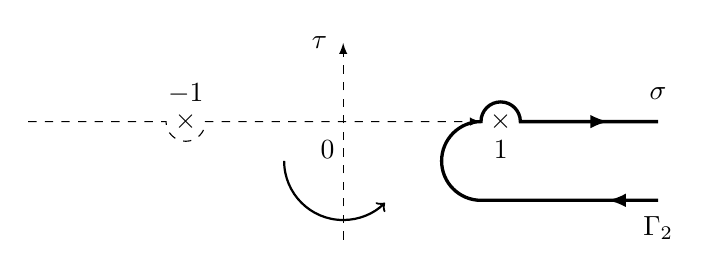
\begin{tikzpicture}
%\node at (-0.5,0) {  $\times$};
\node at (-0.2,-0.35) { $0$};
\node at (2,0) { $\times$}; % Pole
\node at (2,-0.36) { $1$};

\node at (-2,0) { $\times$};
\node at (-2,0.36) {  $-1$}; %pole
\node at (4,-1.35) { $\Gamma_2$};

\draw[dashed, decoration={markings,
 mark=at position 1.0 with {\arrow{latex}}},
      postaction={decorate}] (-4,0) -- (-2.25,0) arc (-180:0:0.25)-- (1.75,0);
      
\node at (4,0.35) {$\sigma$};

\draw[dashed, decoration={markings,
 mark=at position 1.0 with {\arrow{latex}}},
      postaction={decorate}] (0,-1.5) -- (0,1);
\node at (-0.3,1) {$\tau$};      

%\node at (2.5,-0.4) {$(\Gamma_0)$};
      
\draw[ thick, ->] (-0.75,-0.5) arc (0:135:-0.75); 
  

\draw[very thick, black, yshift=0pt,
decoration={ markings,  
      mark=at position 0.1 with {\arrow{latex}},
      mark=at position 0.9 with {\arrow{latex}}},
      postaction={decorate}]
      (4,-1) -- (1.75,-1)  arc (90:-90:-0.5) -- (1.75,0) arc(180:0:0.25)  -- (4,0);
\end{tikzpicture}
\caption
[Contour $\Gamma_2$]
{Contour $\Gamma_2$. The curved arrow shows the deformation of $\Gamma_0$ (dashed line) into $\Gamma_2$.}
\label{chapter5:figure8}
\end{figure}

During this contour deformation, only the poles
\begin{equation}
\lambda = \xi, \quad \text{with } {\rm Im}(\xi) <0 
\end{equation}
of the $DM$ function \eqref{DM_operator} are crossed and therefore, applying the residue theorem, we have for $\xi \in \mathbb{C}$, ${\rm Im}(\xi) <0$, $j=1,2$, 
\begin{equation}
\label{DM_propag_sol}
DM(X_j)(\xi) = \int_{\Gamma_0} DM(\xi,\lambda) X_j(\lambda) \, {\rm d} \lambda  = \int_{\Gamma_2} DM(\xi,\lambda) X_j(\lambda) \, {\rm d} \lambda + m(\xi) X_j(\xi).
\end{equation}

The poles of the $TM$ function \eqref{TM_operator} are
$$ \lambda = T_0^{-1}(\xi) = \xi \, \cos \widetilde{2\varphi}  - \sin \widetilde{2\varphi} \, \zeta_0(\xi) = \cos (\theta - \widetilde{2\varphi}) \quad \text{if} \quad \xi = \cos \theta $$
$T_0^{-1}$ operates in the domain $\Omega_0^-$, therefore they are crossed during this contour deformation if and only if $\xi \in \Omega_0^-$ (see dotted area on Fig.~\ref{chapter5:figure11}).
The domain $\Omega_0^-$ is delineated by the hyperbola 
\begin{equation}
\partial \Omega_0^- = \{   \xi \in \mathbb{C}, \ {\rm Im}(\xi) <0,  \xi = \cos \theta, {\rm Re} \, \theta = \widetilde{2\varphi} \}.
\end{equation}
Domain $\Omega_0^-$ and contour $\partial \Omega_0^-$ are illustrated on Fig.~\ref{chapter5:figure11}.   

Applying the residue theorem to the $TM$ integral operator then gives for $\xi \in \mathbb{C}$, ${\rm Im}(\xi) <0$, $j=1,2$,
\begin{equation}
\label{TM_propag_sol}
TM(X_j)(\xi) = \int_{\Gamma_0} TM(\xi,\lambda) X_j(\lambda) \, {\rm d} \lambda  = \int_{\Gamma_2} TM(\xi,\lambda) X_j(\lambda) \, {\rm d} \lambda + m(\xi) \, X_j[T_0^{-1}(\xi)] \mathbf{1}(\xi \in \Omega_0^-)
\end{equation}

\begin{figure}[ht]%
\begin{center}
	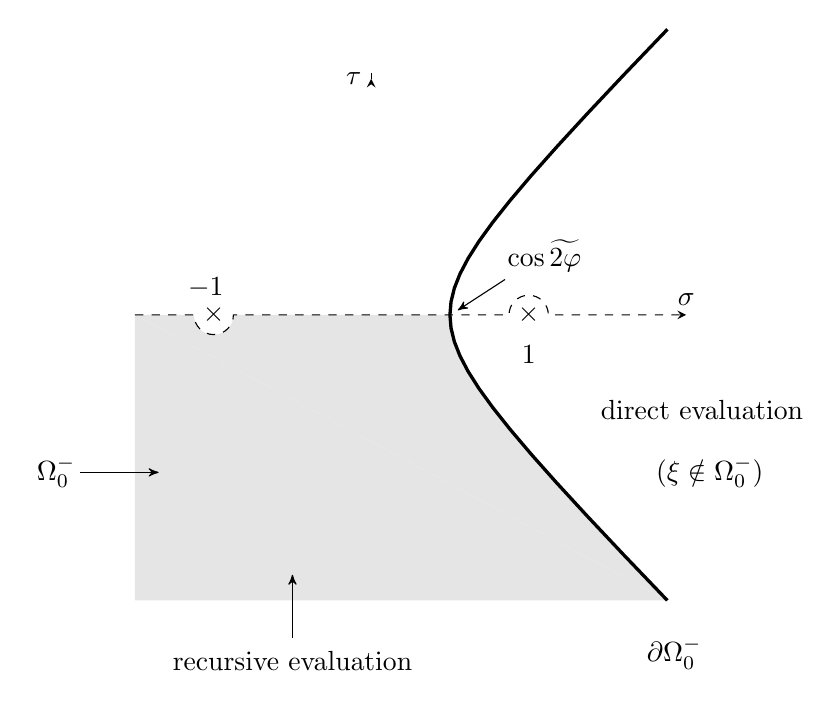
\begin{tikzpicture}
		% Filling Omega_0^-
	\fill [color=gray!20]
	(-1,0)
	-- plot [domain= 0:2] ({cosh(\x)},{-sinh(\x)})
	-- (-3,0)
	-- cycle;
	
	\fill [color=gray!20]
	({cosh(2)},{-sinh(2)})
	-- plot [domain= 0:-3] ({\x},{-sinh(2)})
	-- (-3,0)
	-- cycle;
	
	\fill[color=white] (-2,0) circle (0.25);
	
	\draw[dashed, ->,>=stealth] (-3,0)  -- (-2.25,0) arc(-180:0:0.25)--(1.75,0) arc (180:0:0.25)--(4,0) node[above]{$\sigma$};
	\draw[dashed, ->,>=stealth](0,3)--(0,3) node[left]{$\tau$};
	
	\node at (2,0) {$\times$}; % Pole
	\node at (2,-0.5) {$1$};
	\node at (-2,0) { $\times$};
	\node at (-2.1,0.35) {$-1$}; %pole
	
	% Hyperbola (contour  partial_Omega_0 )
	\draw[black, very thick][domain=-2:2] plot({cosh(\x)}, {-sinh(\x)});
	\node at (3.85,-4.3) {$\partial \Omega_0^-$};
	\draw[thin, ->,>=stealth'](1.7,0.45) -- (1.1, 0.06);
	\node at (2.2, 0.75) {$\cos \widetilde{2\varphi}$};
	
	% Omega_0
	\node at (-4,-2) {$\Omega_0^-$};
	\draw[->,>=stealth'] (-3.7, -2) -- (-2.7,-2);
	\draw[->,>=stealth'] (-1,-4.1) -- (-1,-3.3);
	\node at (-1,-4.4) {recursive evaluation};
	\node at (4.2,-1.2) { direct evaluation};
    \node at (4.3,-2) { $(\xi \notin \Omega_0^-)$};
	
	\end{tikzpicture}
\end{center}
\caption
[Domain $\Omega_0^-$ and its lower boundary $\partial \Omega_0^-$]
{Domain $\Omega_0^-$ and its lower boundary $\partial \Omega_0^-$ in the complex plane $\xi=\sigma + i \tau$. $\Omega_0^-$ is delimited by $\partial \Omega_0^-$ andthe semi-axis $]-\infty, \cos \widetilde{2\varphi}]$. }
\label{chapter5:figure11}
\end{figure}


Using \eqref{DM_propag_sol} and \eqref{TM_propag_sol} in the system of functional equations \eqref{sys_regular}, the system \eqref{sys_regular} is then equivalent to this new system for $\xi \in \mathbb{C}$, ${\rm Im}(\xi) <0$:
\begin{equation}
\label{propag_sol_sys}
\begin{cases}
X_1(\xi) = g_1(\xi) -  X_2(T_0^{-1}(\xi)) \, \mathbf{1}(\xi \in \Omega_0^-) \\
\\
X_2(\xi) = g_2(\xi) - X_1(T_0^{-1}(\xi)) \, \mathbf{1}(\xi \in \Omega_0^-) 
\end{cases}
\end{equation}
where
\begin{equation}
g_j(\xi) = m(\xi)^{-1} \left[ u_j(\xi) - \int_{\Gamma_2} DM(\xi,\lambda) \, X_j(\lambda) \, {\rm d} \lambda - \int_{\Gamma_2} TM(\xi,\lambda) \, X_{3-j}(\lambda) \, {\rm d} \lambda \right] \\
\end{equation}
Formula \eqref{propag_sol_sys} is called the recursive formula because it uses the value of the regular function $X_2$ at point $T_0^{-1}(\xi)$ to compute the value of $X_1$ at the point $\xi$ where the approximation is not valid (and vice-versa). If the translation from $\xi$ to $T_0^{-1}(\xi)$ is not sufficient to reach the domain $\mathbb{C} \backslash \Omega_0^-$ where the approximation is valid, then the use of the formula is repeated as many times as necessary (computing $X_2(T_0^{-1}(\xi))$ using the value of $X_1(T_0^{-2}(\xi))$, etc.).

To calculate $g_j$ functions, we need to compute
\begin{equation*}
\int_{\Gamma_2} DM(\xi,\lambda) \, X_j(\lambda) {\rm d} \lambda =\sum_k \tilde{X}_j^k \int_{\Gamma_2} DM(\xi,\lambda) \, \varphi_k(\lambda) \, {\rm d} \lambda 
\end{equation*}
and
\begin{equation*}
\int_{\Gamma_2} TM(\xi,\lambda) \, X_j(\lambda) {\rm d} \lambda = \sum_k \tilde{X}_j^k \int_{\Gamma_2} TM(\xi,\lambda) \, \varphi_k(\lambda) \, {\rm d} \lambda
\end{equation*}

If ${\rm Im}(a) < 0$, the residue theorem combined with the variable change $\lambda = iy$  yields
\begin{equation}
\int_{\Gamma_2} DM(\xi,\lambda) \,  \dfrac{1}{\lambda+a} \, \, {\rm d} \lambda =  \dfrac{1}{2\pi} \, \mathcal{D}(a,\xi) - \dfrac{m(\xi)}{\xi +a} = \mathcal{ND}(a,\xi). 
\end{equation}

For the $TM$ contributions, the poles $\lambda = T_0^{-1}(\xi)$ are taken into account if and only if $\xi \in \Omega_0^-$. Thus, for $\xi \in \Omega_0^-$, ${\rm Im}(a) < 0$, the residue theorem combined with the variable change $\lambda = iy$ gives
\begin{equation}
\int_{\Gamma_2} TM(\xi,\lambda) \,  \dfrac{1}{\lambda +a} \, \, {\rm d} \lambda = \frac{1}{2i\pi} \mathcal{T}(a,\xi)- \dfrac{m(\xi)}{T_0^-(\xi) +a}   =  \mathcal{NT}(a,\xi)
\end{equation}

Formula \eqref{regular_part_decomp} finally leads to, for $\xi \in \Omega_0^-$ and $j=1,2$,
\begin{eqnarray}
m(\xi)\, g_j(\xi) -  u_j(\xi)=
-\Big( \sum_k \tilde X_j^{k}\, d_k \, N\mathcal D(a_k,\xi)+\sum_k \tilde X_{3-j}^{k} \, d_k \,
N\mathcal T(a_k,\xi) \Big) \nonumber
\end{eqnarray}

Some numerical results are presented in the sequel.

\section{Numerical results}
\label{Chapter5:results}

In this section, a far-field ($k_0r>>1$) asymptotic evaluation of the diffraction coefficient is computed using the stationary phase method :
\begin{equation}
\label{GTDCoeff_SF}
D(\theta) = \dfrac{e^{-i\frac{\pi}{4}}}{\sqrt{2\pi}} \, [\hat{\alpha}_1( - \cos \theta) + \hat{\alpha}_2( - \cos ( 2\varphi - \theta))]
\end{equation}
where $\hat{\alpha}_1$ and $\hat{\alpha}_2$ are the spectral functions, is compared to the analytic expression of the diffraction coefficient of the scattering of a plane wave with a wedge at interfaces fluid/void as expressed by Sommerfeld \cite{Sommerfeld}. Keller \cite{GTD} gives an analytical expression of the GTD approximation of the coefficient in the case of the diffraction of a scalar plane wave by a wedge with Dirichlet boundaries which can be used in the case of a stress-free wedge immersed in a fluid :
\begin{align}
\label{GTDCoeff_Dir}
D^{\rm (Dir)}(\theta) = \dfrac{e^{i\frac{\pi}{4}}}{2N \sqrt{2\pi}}  \, \left[ \cot \left( \dfrac{\pi + (\theta + \theta_{\rm inc})}{2N} \right) + \cot \left( \dfrac{\pi - (\theta + \theta_{\rm inc})}{2N} \right) \right.   \nonumber \\
\left. - \cot \left( \dfrac{\pi + (\theta - \theta_{\rm inc})}{2N} \right) - \cot \left( \dfrac{\pi - (\theta - \theta_{\rm inc})}{2N} \right) \right],
\end{align}
with $N=2\varphi/\pi$.

To apply the recursive procedure described in \ref{propag_sol}, calculation points $\xi$ must have a negative imaginary part. The calculation points considered are then
\begin{equation}
\label{calculation_points_recursive}
\xi_1 = -\cos \theta -i\,10^{-3}  \quad \text{and} \quad \xi_2=- \cos (2\varphi - \theta) - i\, 10^{-3} ,
\end{equation}
where $\theta$ is the observation angle in the wedge (see Fig.~\ref{chapter5:figure1}).

For the Galerkin basis defined in \eqref{Galerkin_basis}, the parameters $a_k \in [1,\infty[$ are chosen as an exponential law \cite{CroisilleLebeau}:
\begin{equation}
\begin{split}
\label{bas_Gal}
a_k &= 1.1 + 0.05 \left( 10^{\frac{k -1}{4}} - 1 \right), \quad 1\leq k\leq 20 \\
b_k &= a_k  - i 0.1, \quad 1\leq k\leq 20 .
\end{split}
\end{equation}

The module of the diffraction coefficients computed using spectral functions and Sommerfeld integral method for various wedge angles are plotted in terms of the observation angle $\theta, \quad 0\leq \theta\leq 2\varphi$ and presented on Fig.~\ref{chapter5:figure12}. 
\begin{figure}[h!]
\centering
\begin{subfigure}[b]{0.49\textwidth}
        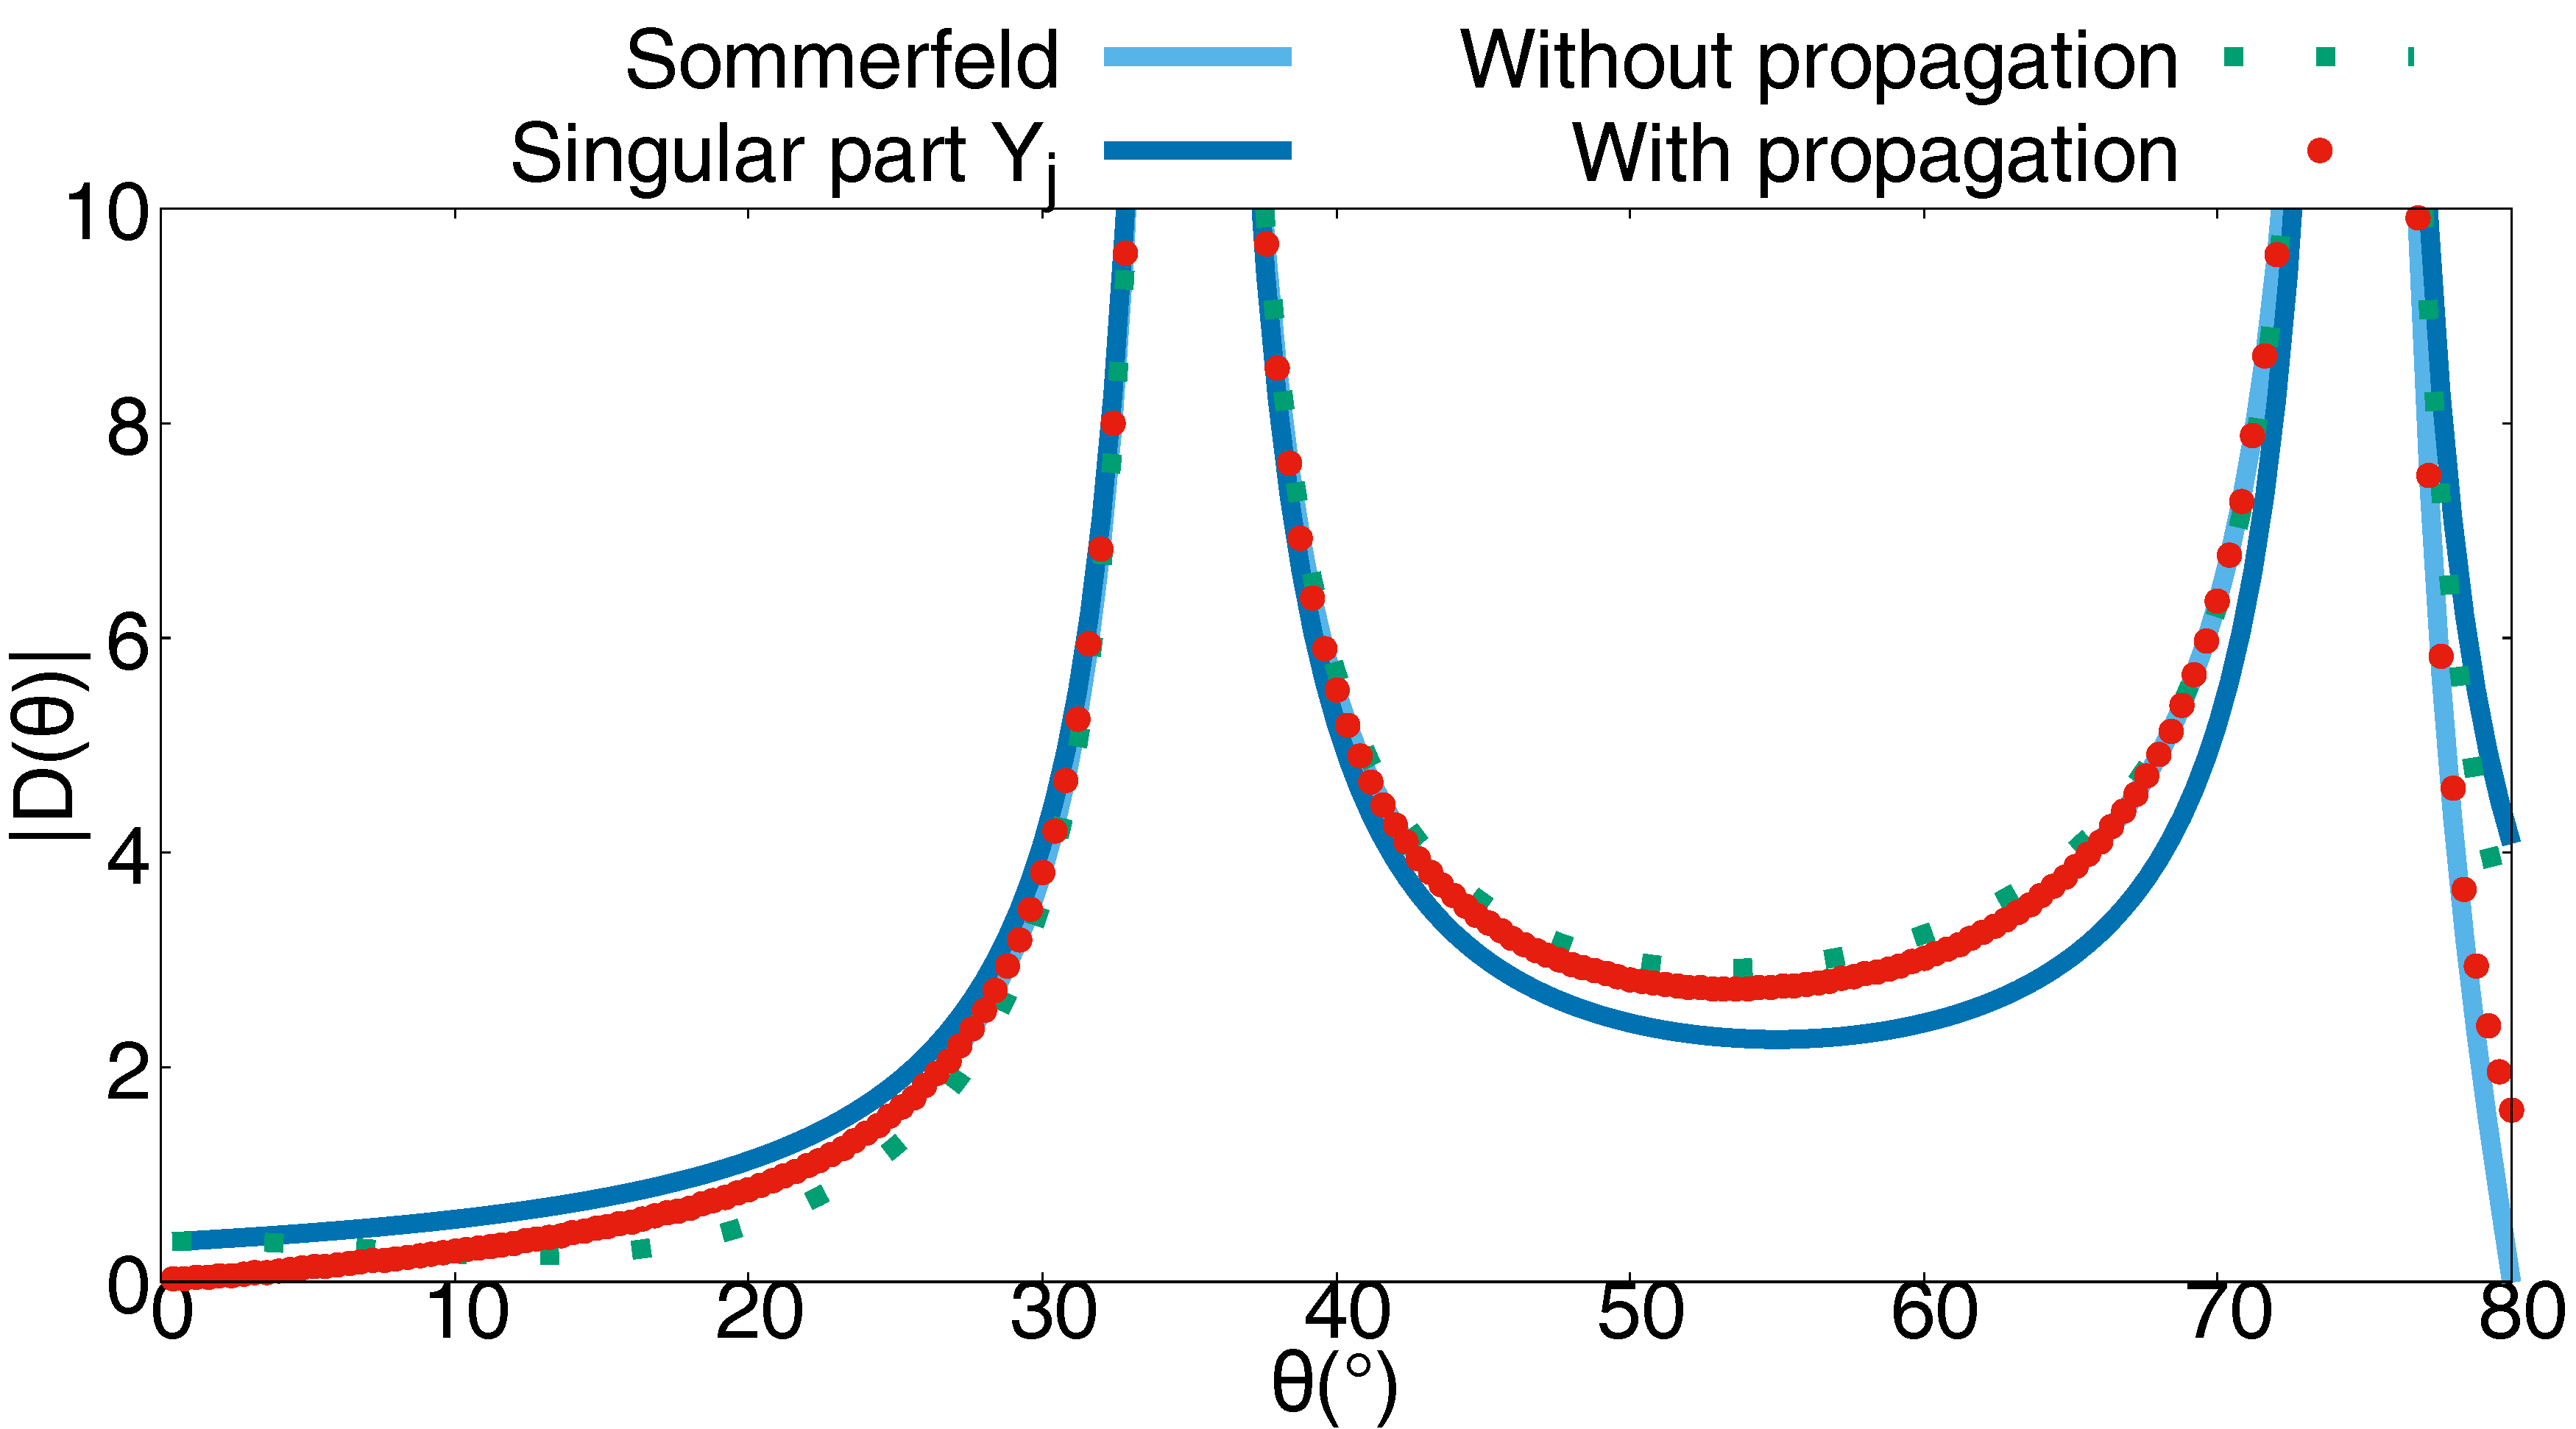
\includegraphics[width=\textwidth]{images/chapter2/Figure8a.pdf}
        \caption{$2\varphi = 80^o$, $\theta_{\rm inc} = 55^o$}
        \label{chapter5:figure12a}
    \end{subfigure}
\begin{subfigure}[b]{0.49\textwidth}
        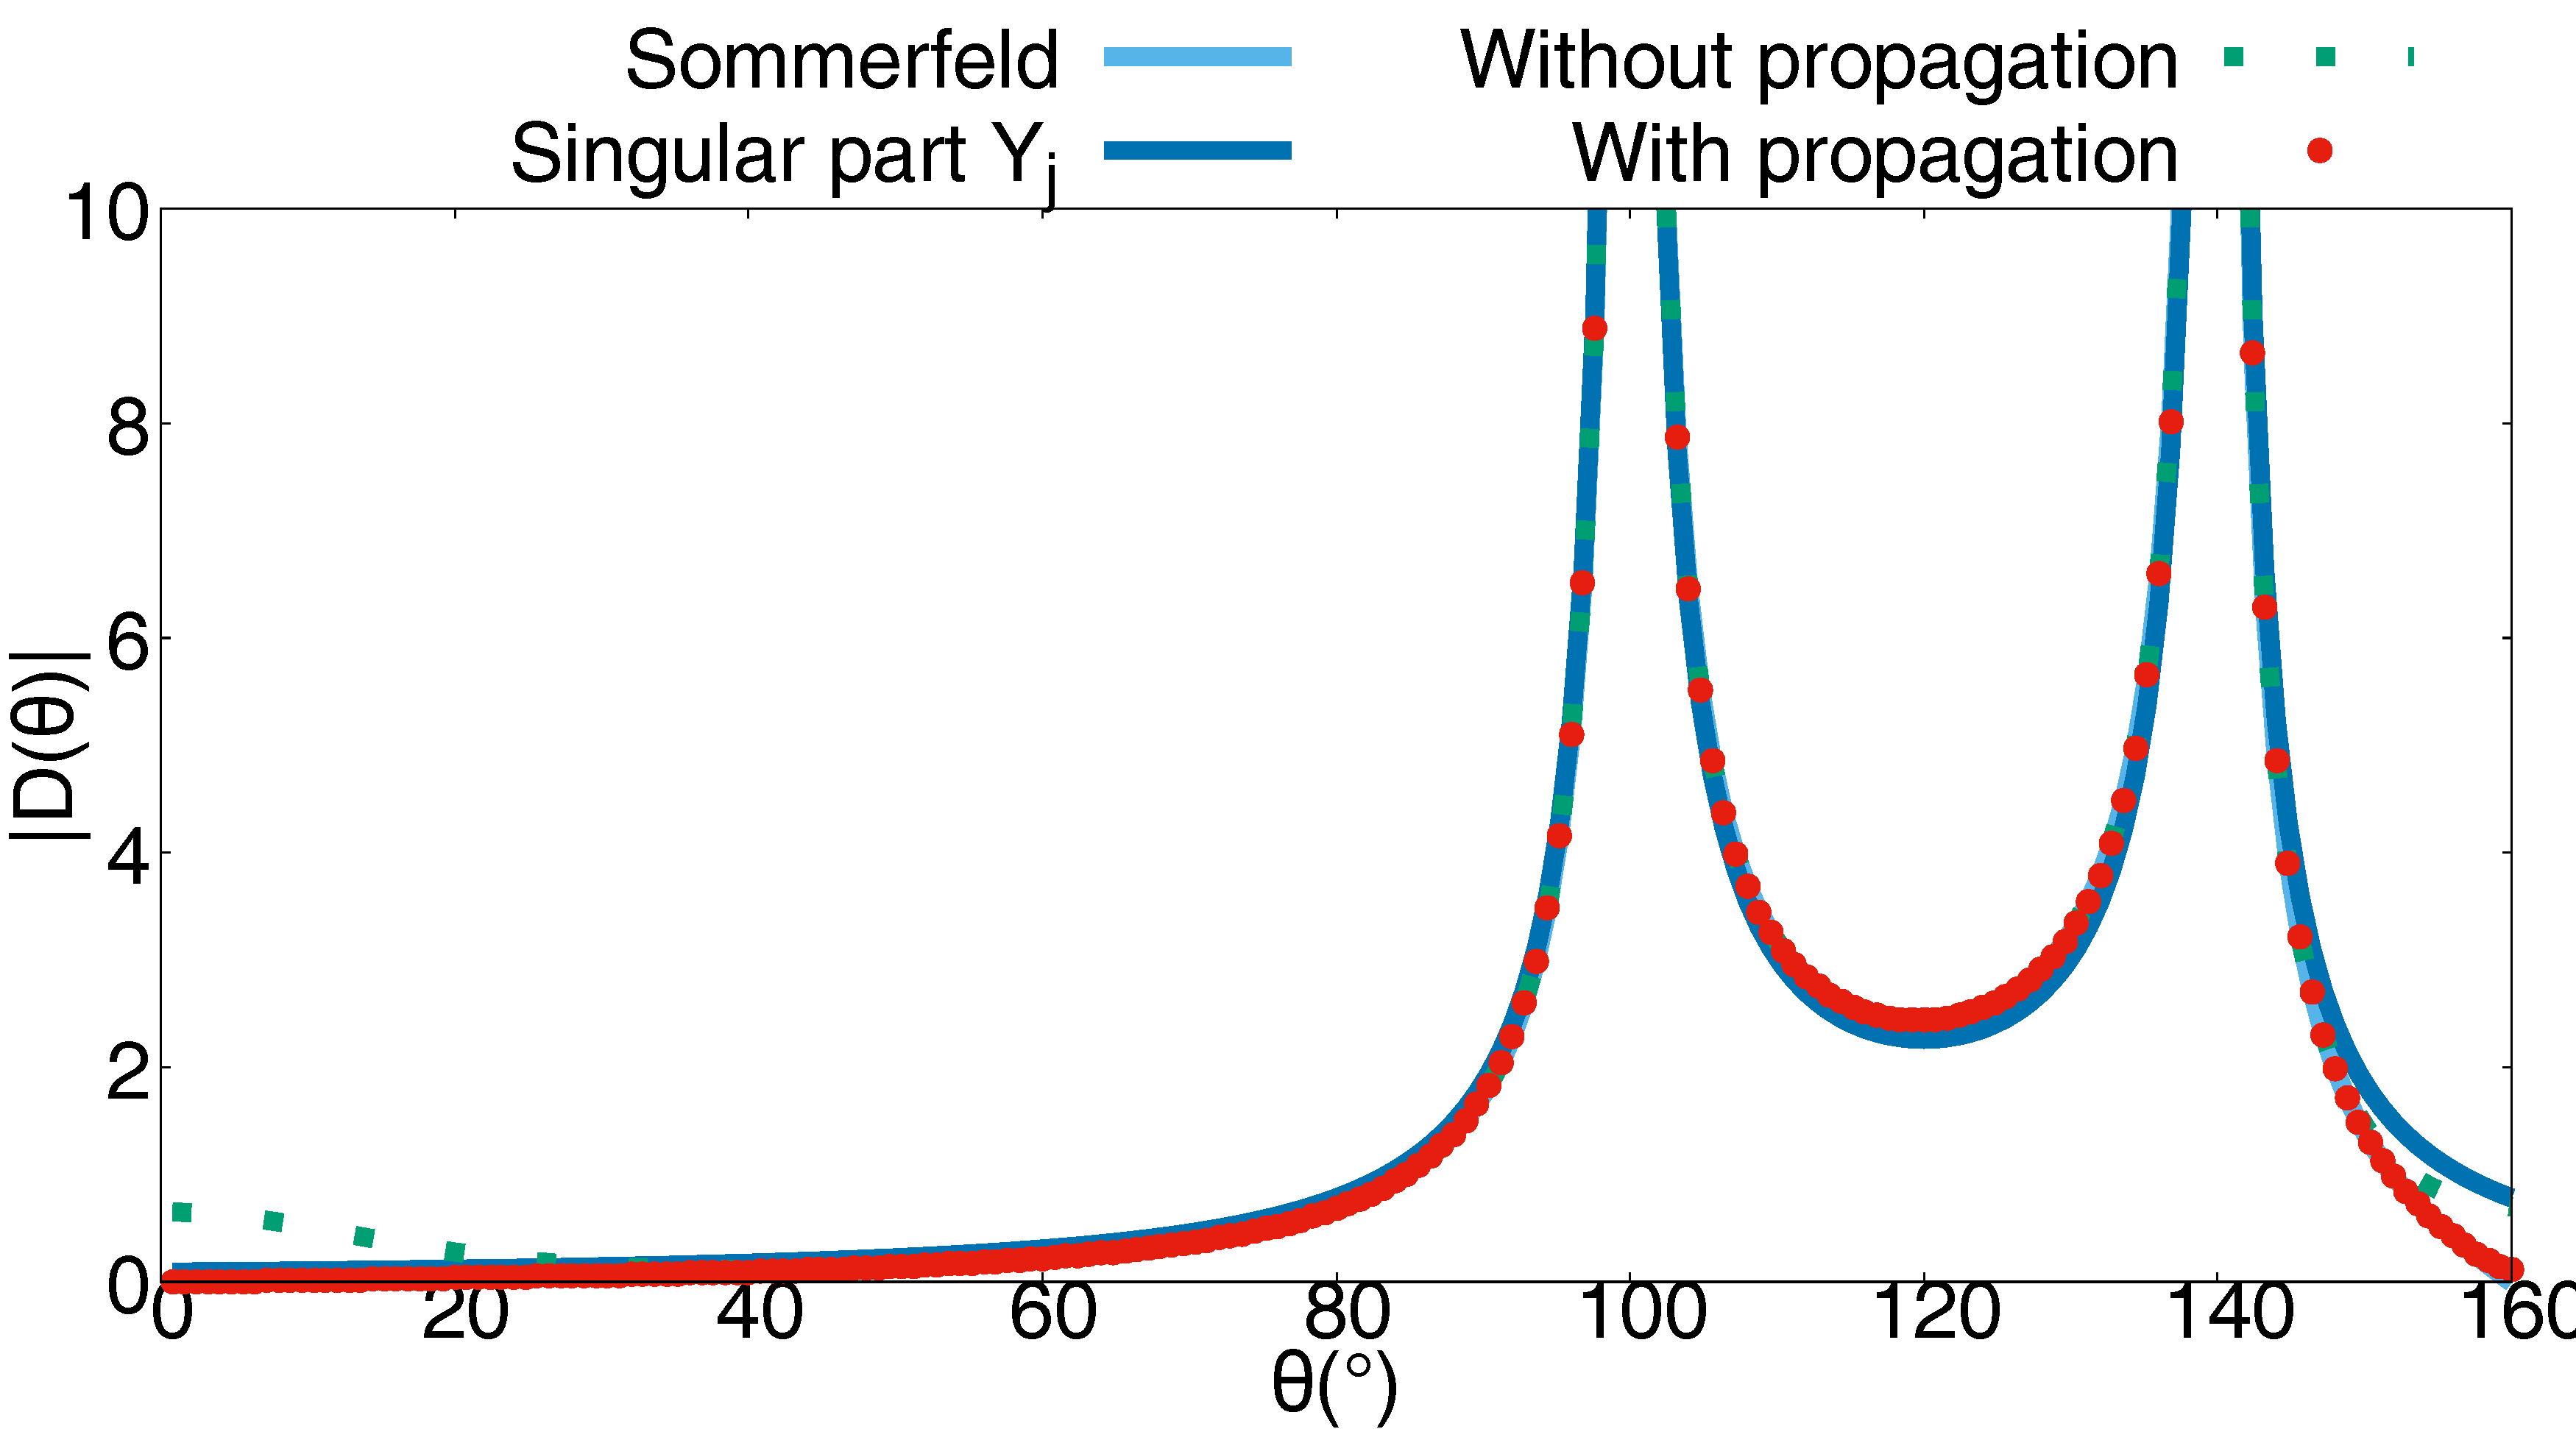
\includegraphics[width=\textwidth]{images/chapter2/Figure8b.pdf}
        \caption{$2\varphi = 160^o$, $\theta_{\rm inc} = 40^o$}
        \label{chapter5:figure12b}
    \end{subfigure}
\\
~\\
\begin{subfigure}[b]{0.49\textwidth}
        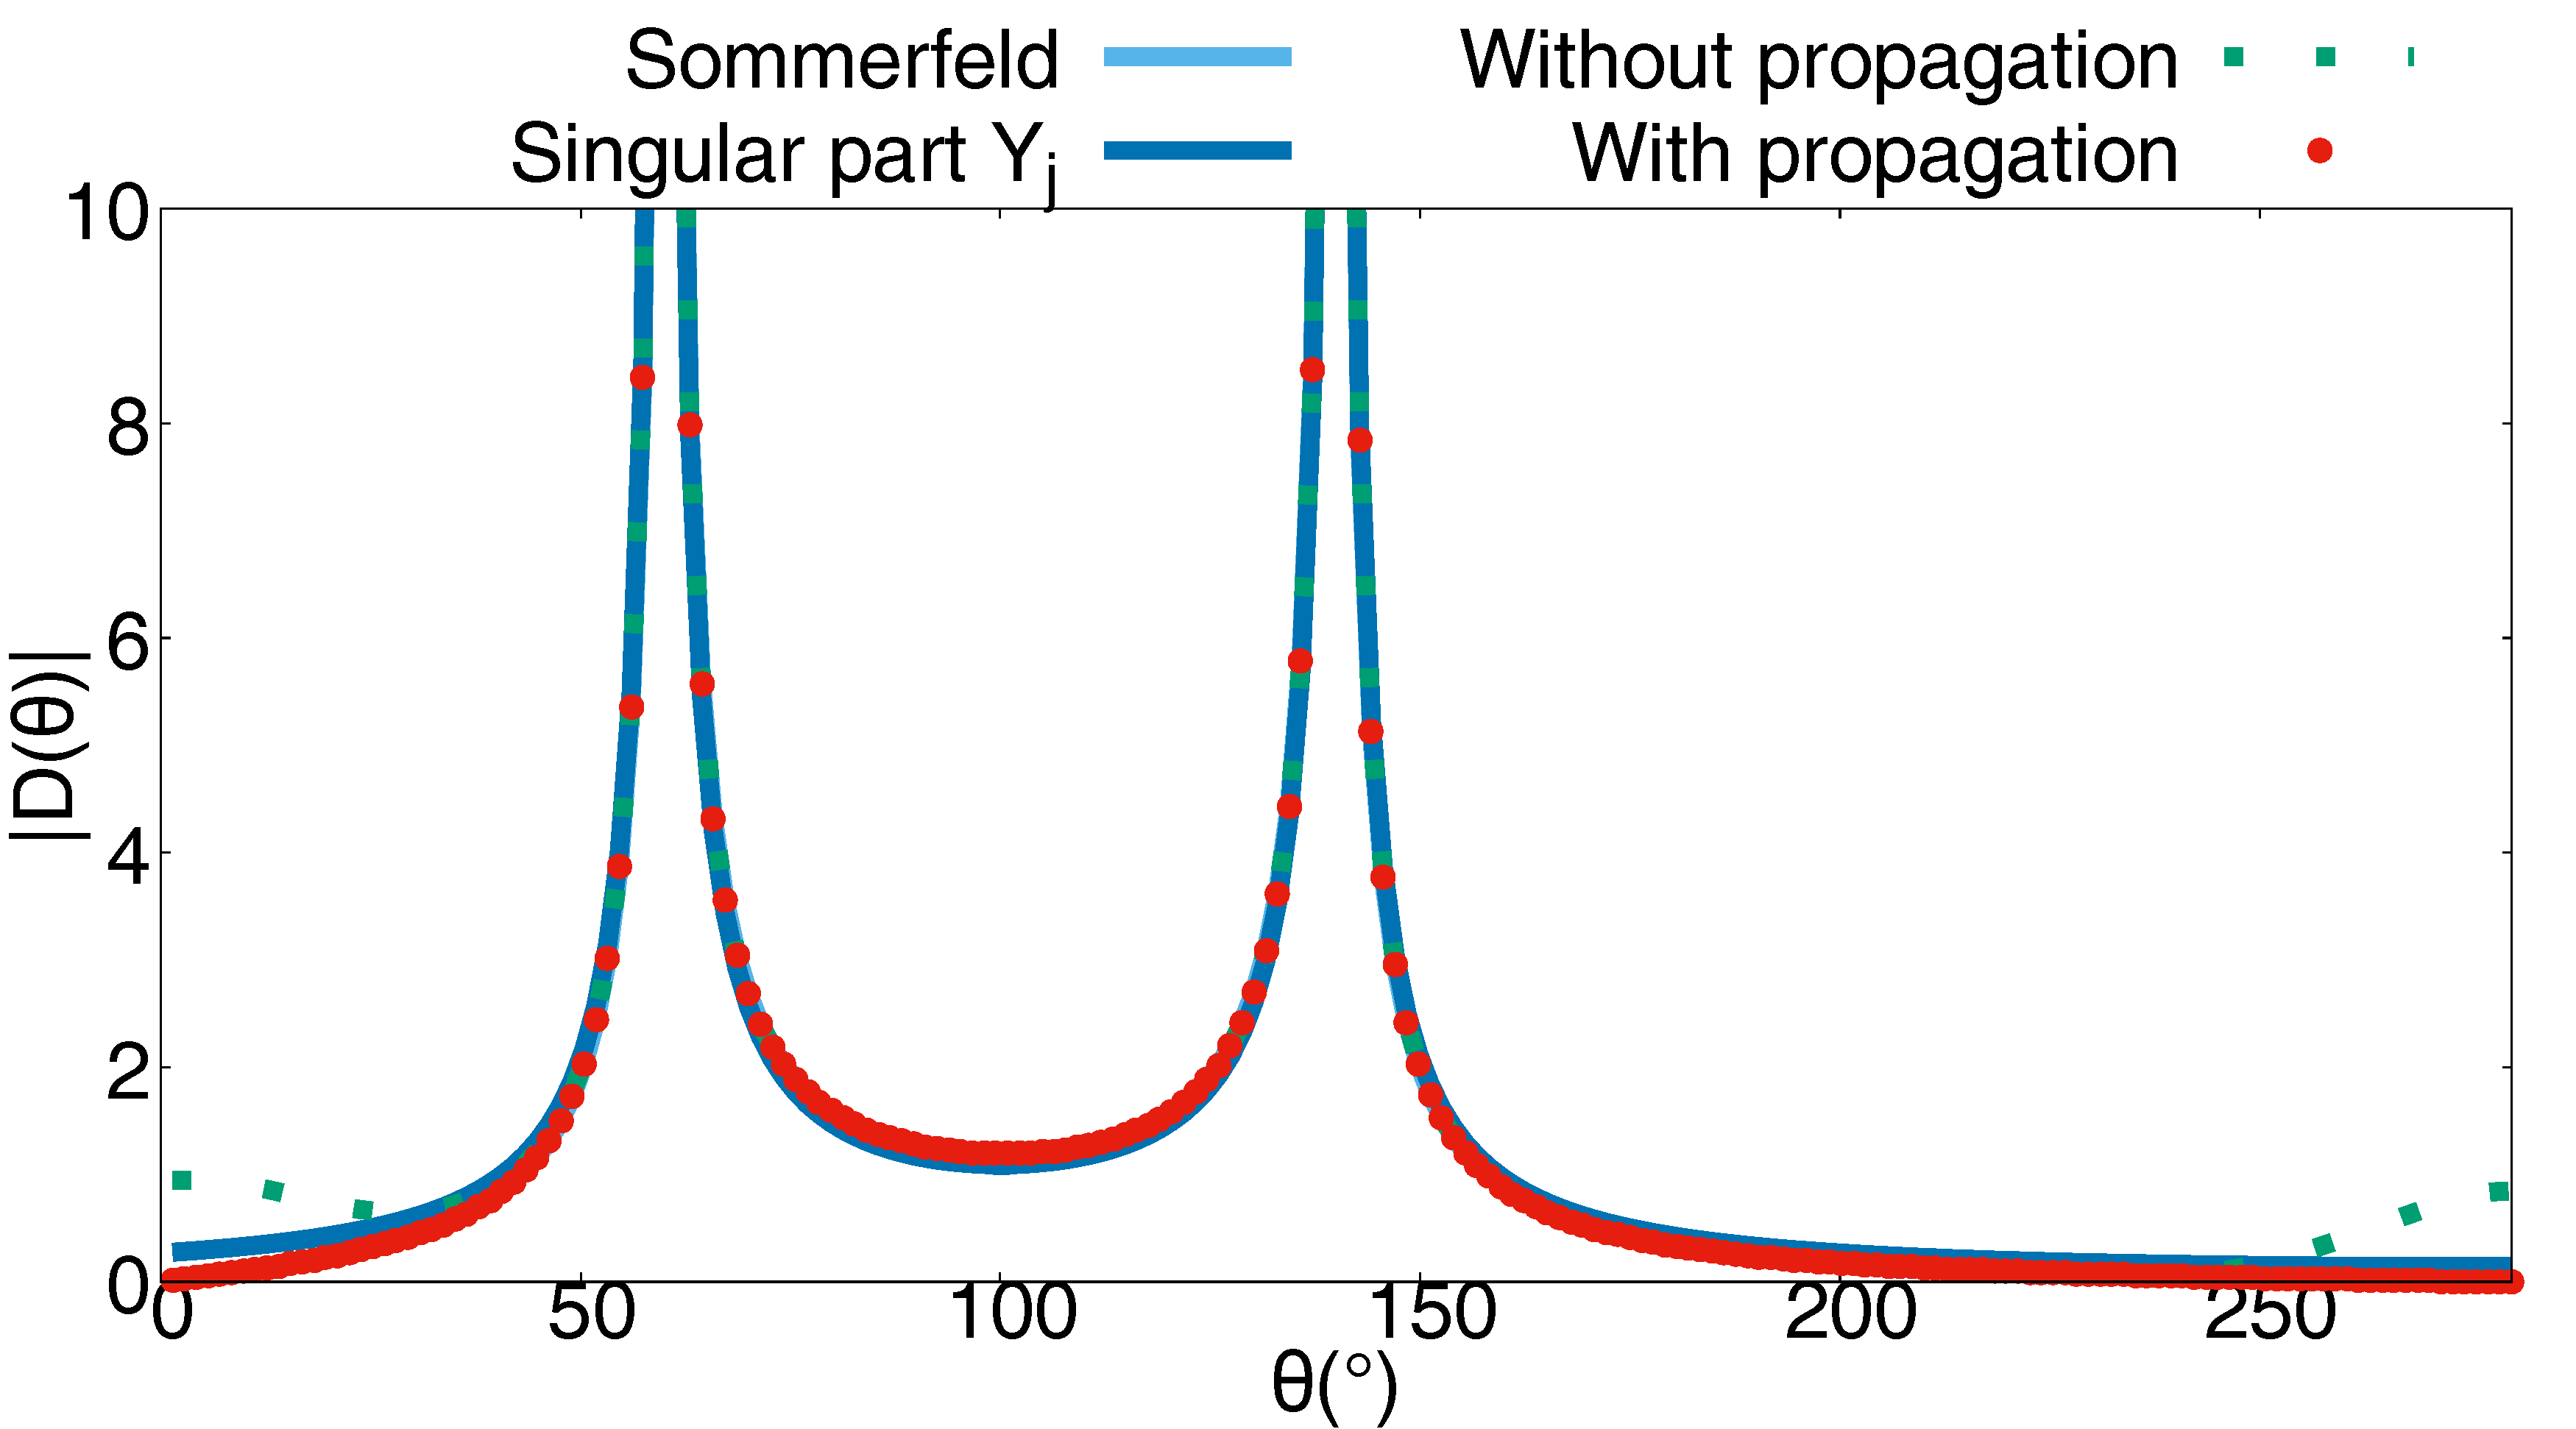
\includegraphics[width=\textwidth]{images/chapter2/Figure8c.pdf}
        \caption{$2\varphi = 280^o$, $\theta_{\rm inc} = 240^o$}
        \label{chapter5:figure12d}
    \end{subfigure}
\begin{subfigure}[b]{0.49\textwidth}
        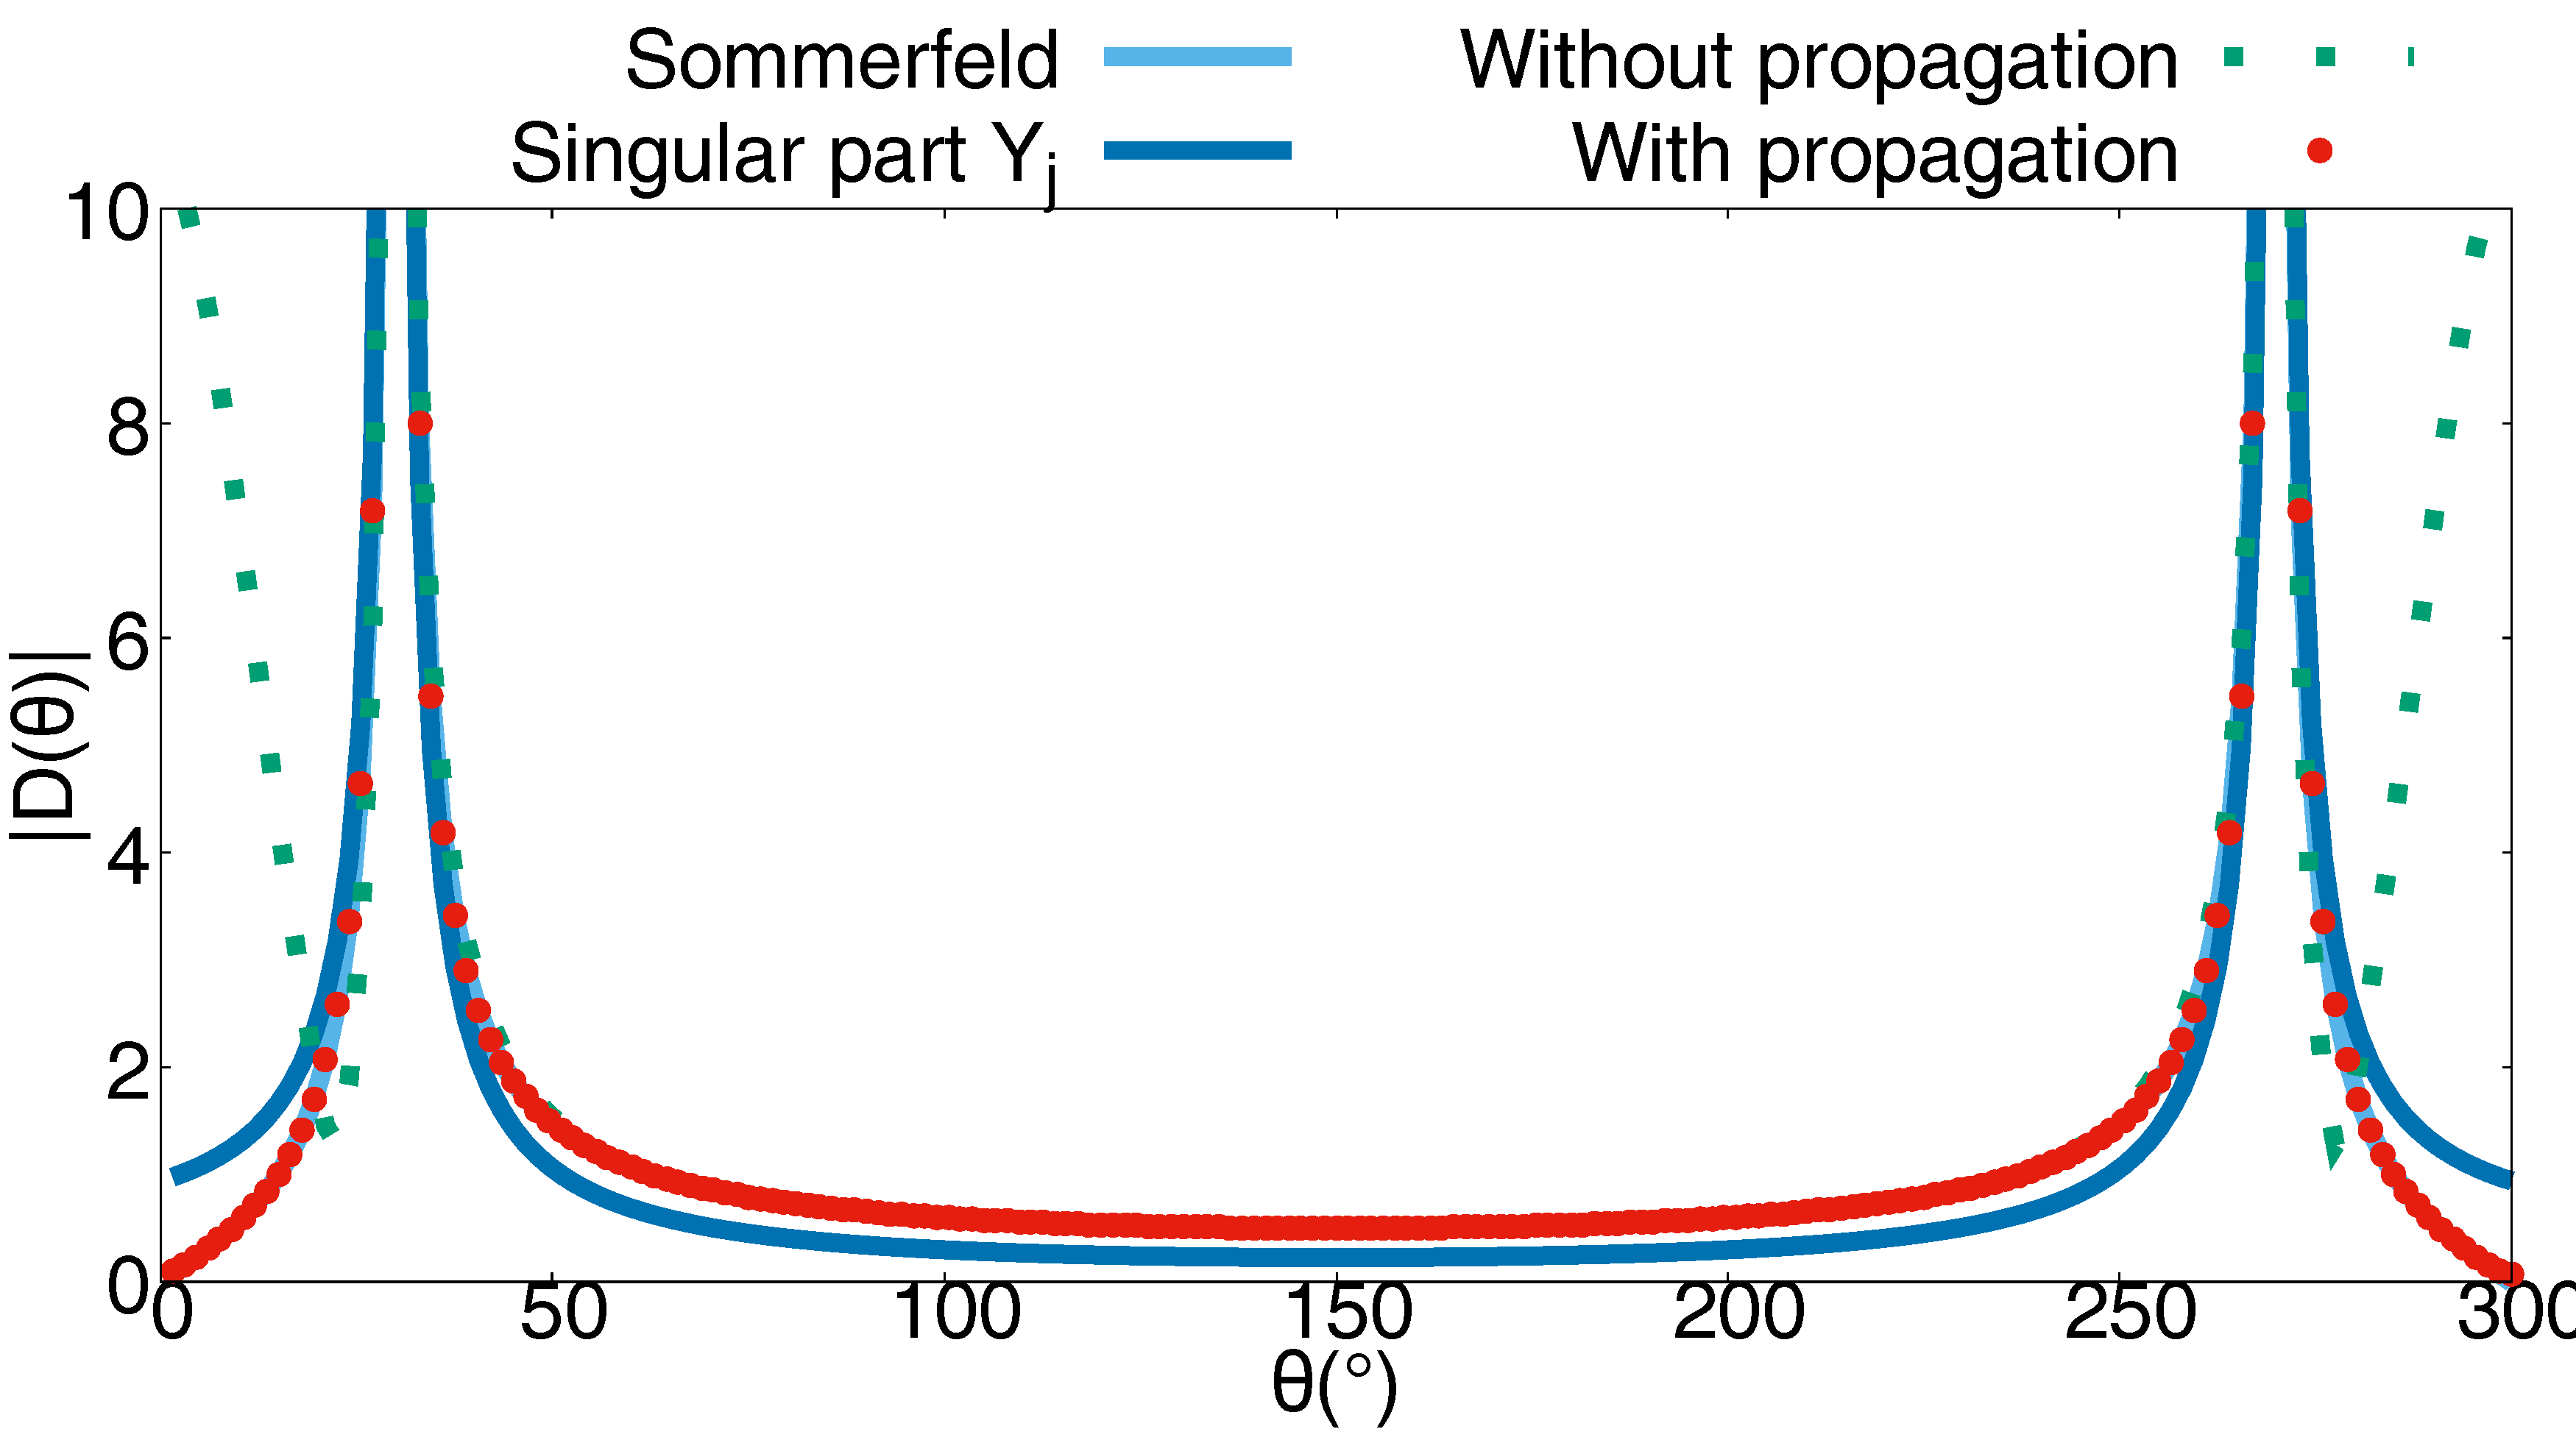
\includegraphics[width=\textwidth]{images/chapter2/Figure8d.pdf}
        \caption{$2\varphi = 300^o$, $\theta_{\rm inc} = 150^o$}
        \label{chapter5:figure12c}
    \end{subfigure}
\caption
[Diffraction coefficient computed with the recursive formula of spectral functions and with the Sommerfeld method, in the case of Dirichlet boundary conditions]
{Diffraction  coefficient computed with the spectral functions and with the Sommerfeld method, in the case of Dirichlet boundary conditions.}
\label{chapter5:figure12}
\end{figure}

In the case of Neumann boundary conditions, the initial system \eqref{Chapter5:Adimen_waveMotion} is replaced by the follwing :
\begin{equation}
\begin{cases}
(\triangle+1)v =  0 \quad \text{in } \Omega_f, \\
\partial v/\partial n =  -\partial h_{\rm inc}/\partial n \quad \quad \quad \text{on } F_j, \quad j=1,2
\end{cases},
\label{neuproblem}
\end{equation}
where n is the inward-pointing normal to the wedge faces. The spectral functions method can once again be applied following the same steps as for the Dirichlet boundary conditions. The details of the computation are not repeated here. Once again, a far-field evaluation of the diffraction, given by  \eqref{GTDCoeff_SF} is compared to the analytic expression of the diffraction coefficient given by Sommerfeld \cite{Sommerfeld}. The GTD approximation of this coefficient is also given by Keller \cite{GTD} :
\begin{align}
\label{GTDCoeff_Neu}
D^{\rm (Neu)}(\theta) = \dfrac{e^{i\frac{\pi}{4}}}{2N \sqrt{2\pi}}  \, \left[ \cot \left( \dfrac{\pi + (\theta + \theta_{\rm inc})}{2N} \right) + \cot \left( \dfrac{\pi - (\theta + \theta_{\rm inc})}{2N} \right) \right.   \nonumber \\
\left. + \cot \left( \dfrac{\pi + (\theta - \theta_{\rm inc})}{2N} \right) + \cot \left( \dfrac{\pi - (\theta - \theta_{\rm inc})}{2N} \right) \right] 
\end{align}
with $N=2\varphi/\pi$. The results are presented on Fig ~\ref{chapter5:figure13}.

\begin{figure}[h!]
\centering
\begin{subfigure}[b]{0.49\textwidth}
        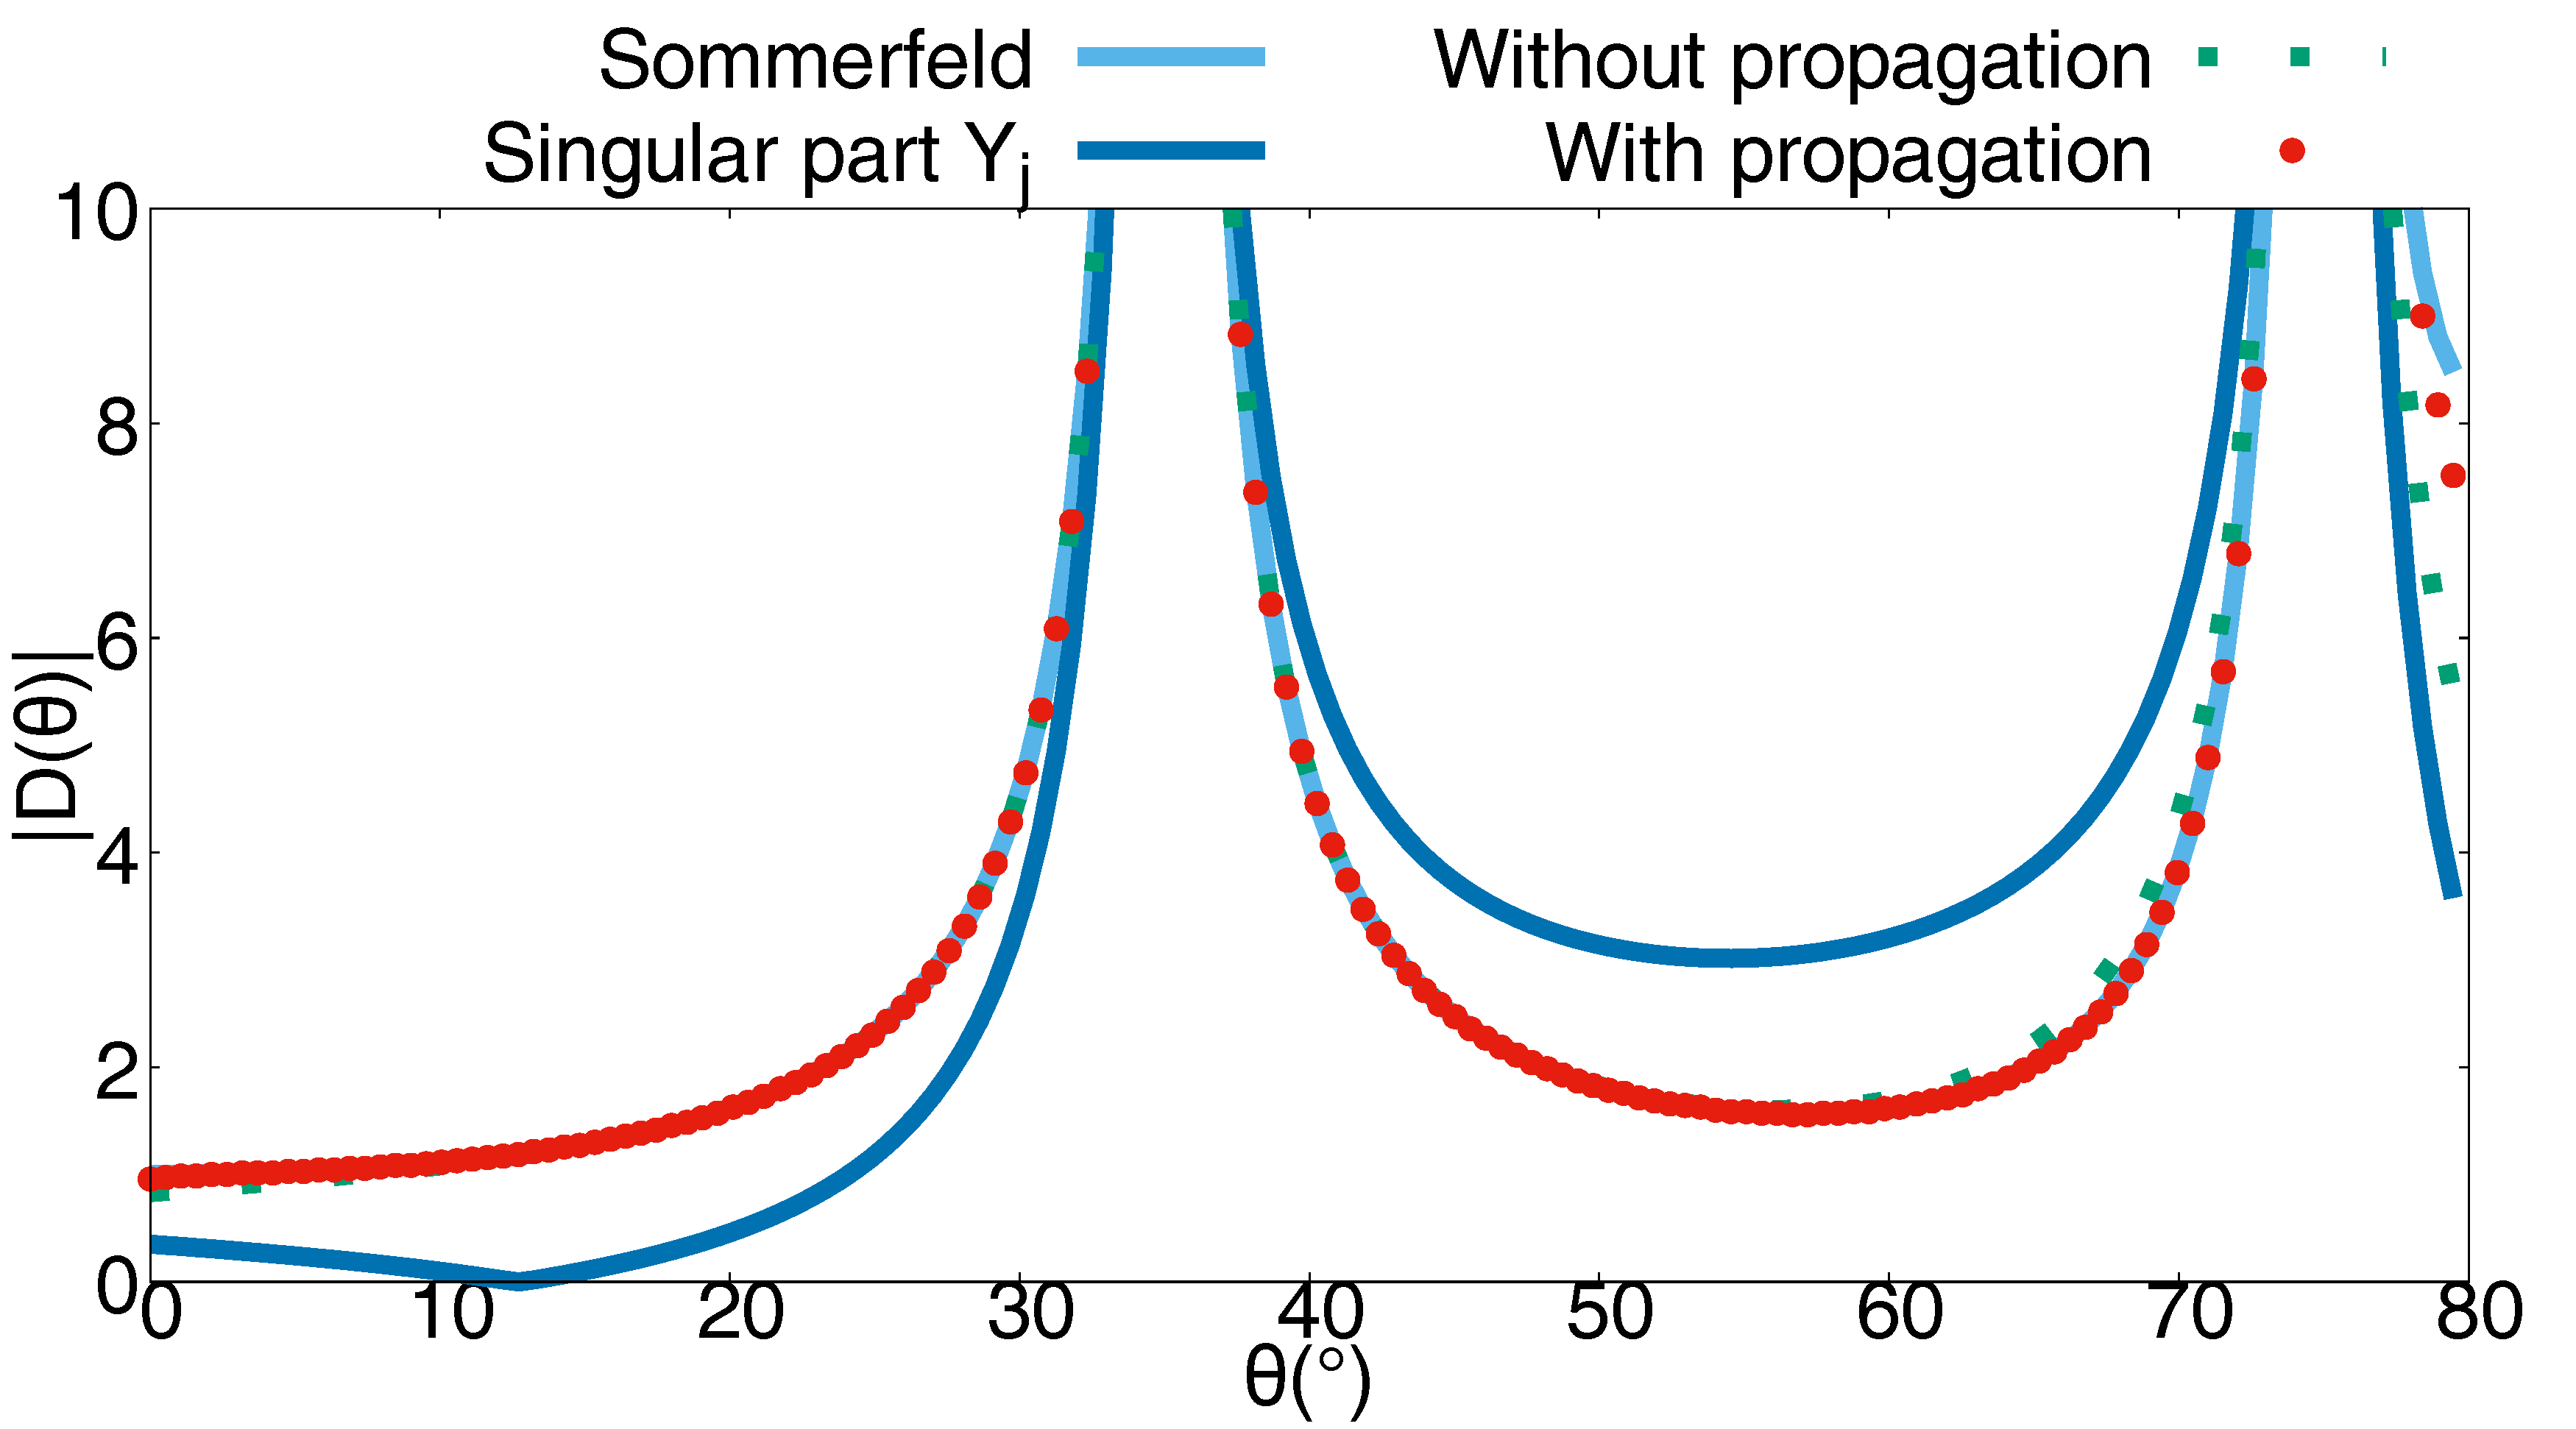
\includegraphics[width=\textwidth]{images/chapter2/Figure9a.pdf}
        \caption{$2\varphi = 80^o$, $\theta_{\rm inc} = 55^o$}
        \label{chapter5:figure13a}
    \end{subfigure}
\begin{subfigure}[b]{0.49\textwidth}
        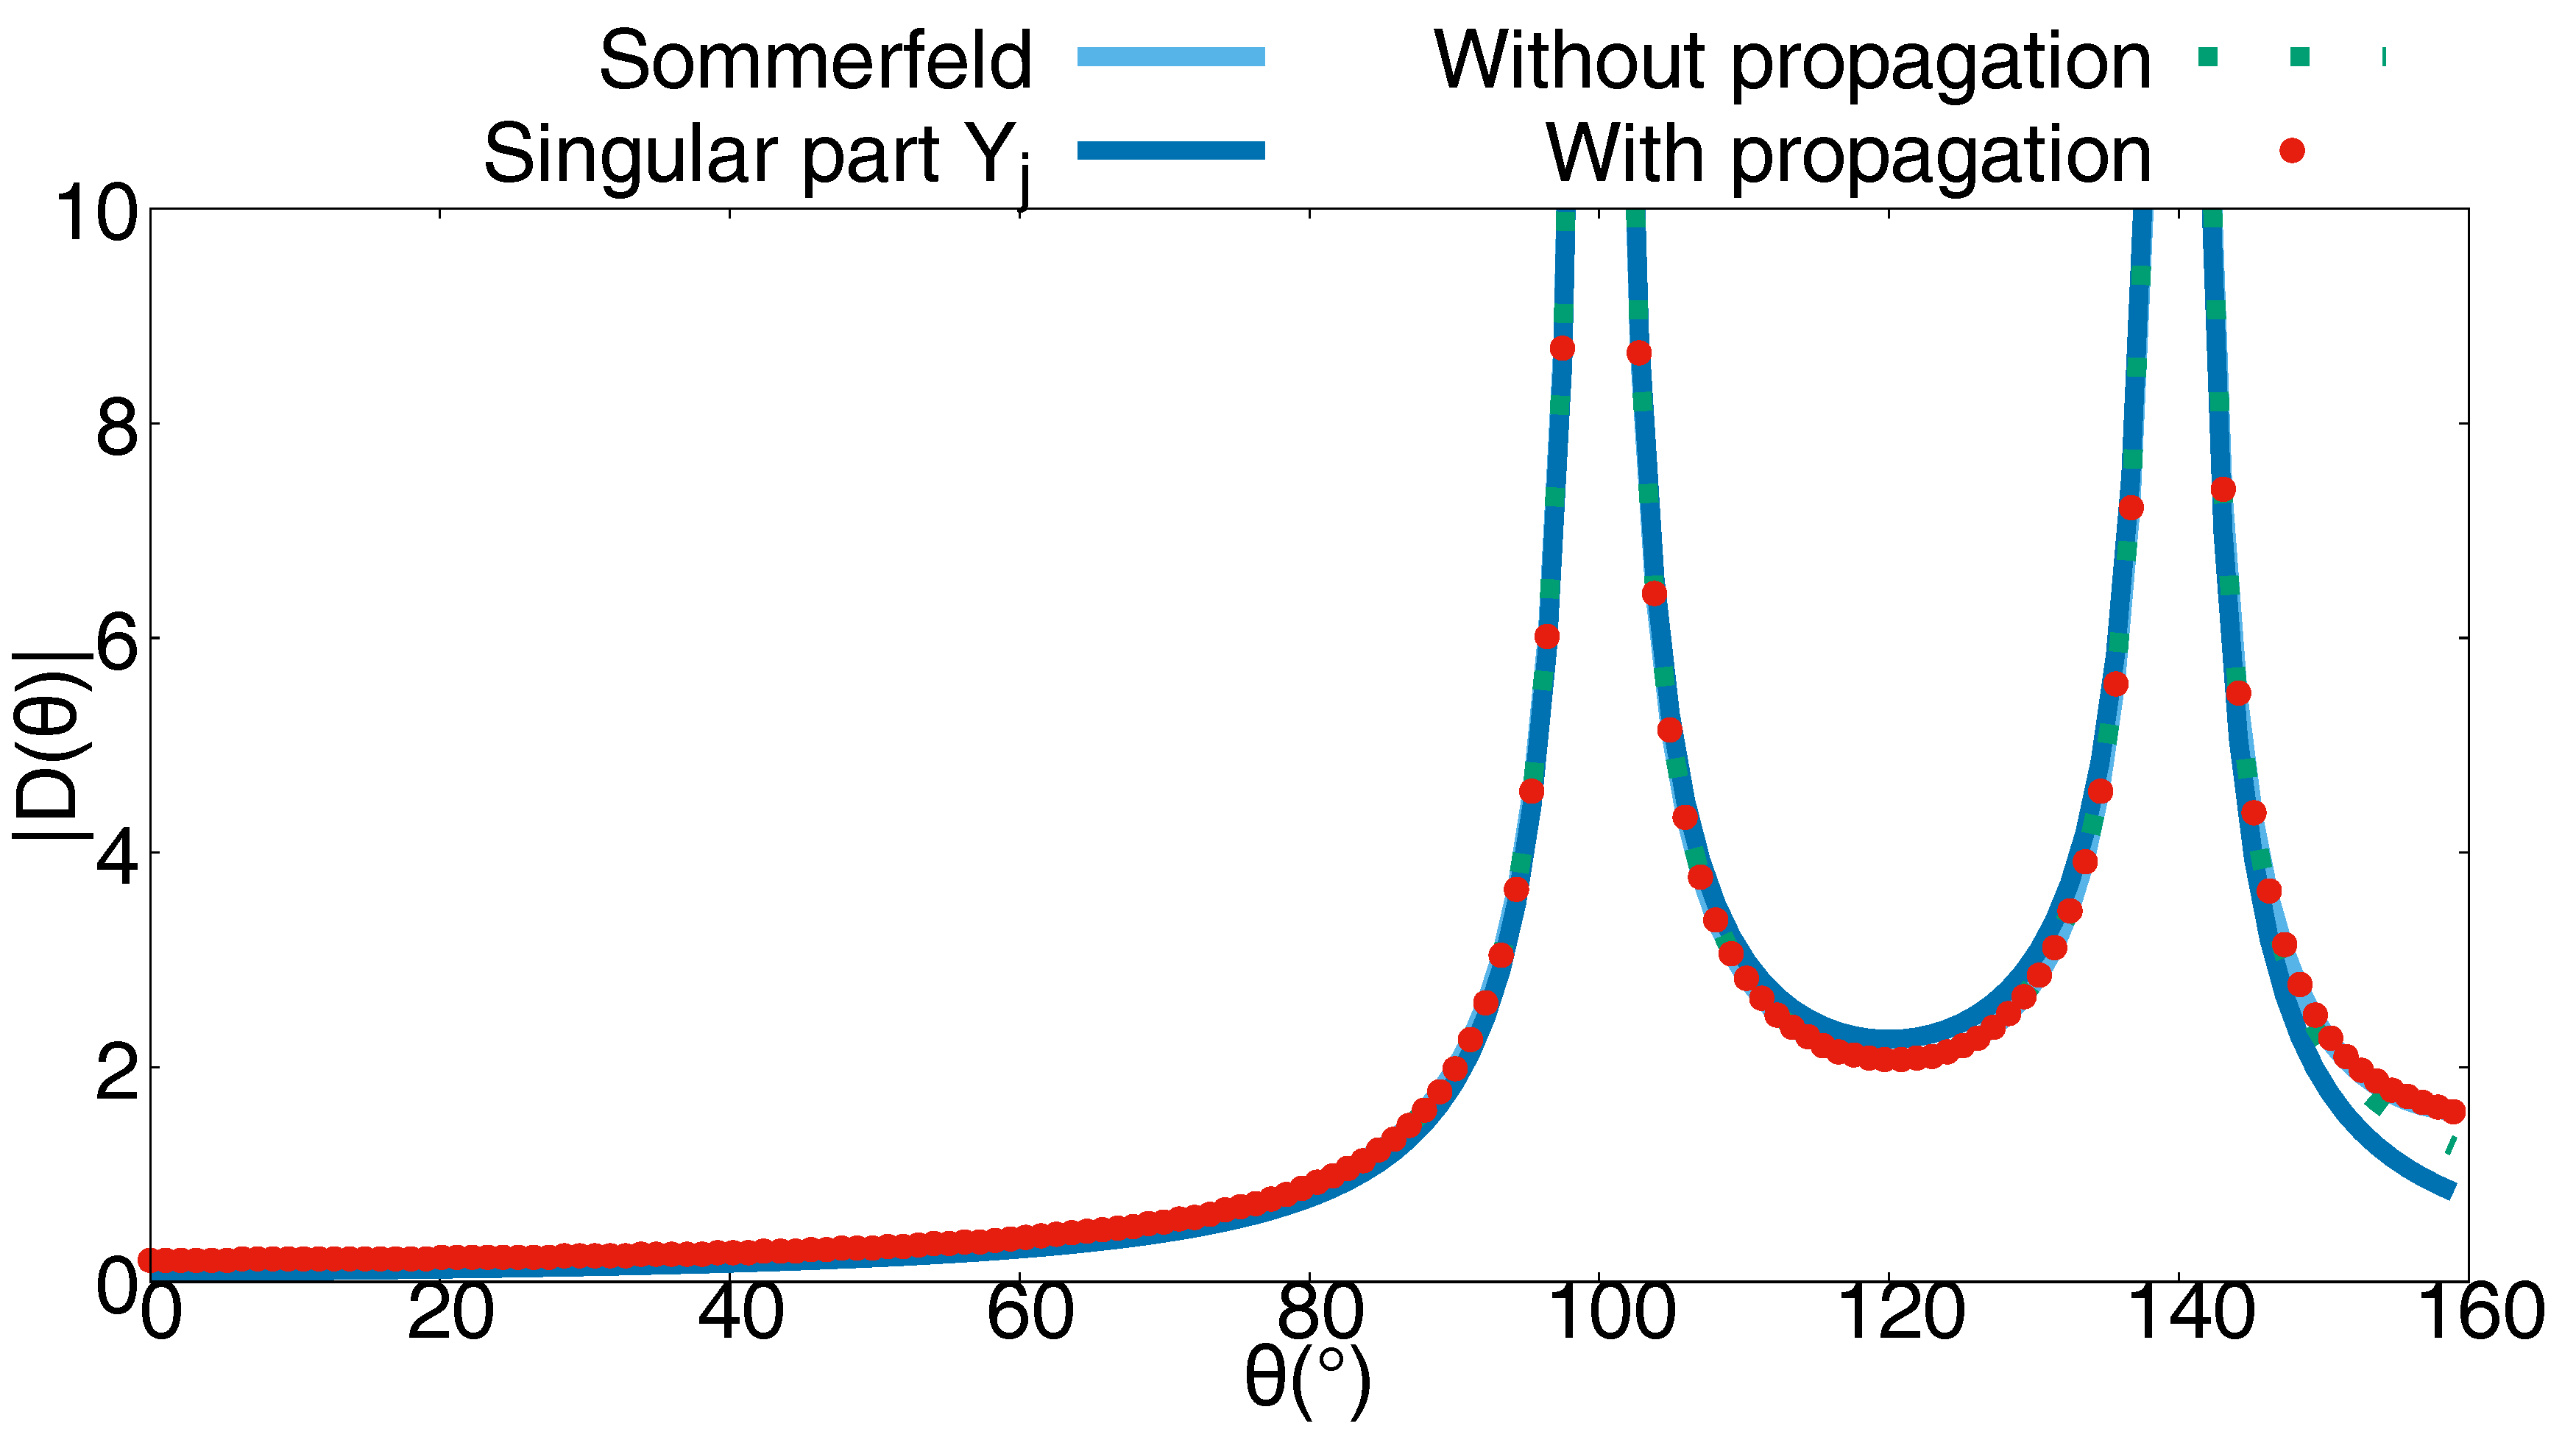
\includegraphics[width=\textwidth]{images/chapter2/Figure9b.pdf}
        \caption{$2\varphi = 160^o$, $\theta_{\rm inc} = 40^o$}
        \label{chapter5:figure13b}
    \end{subfigure}
\\
~\\
\begin{subfigure}[b]{0.49\textwidth}
        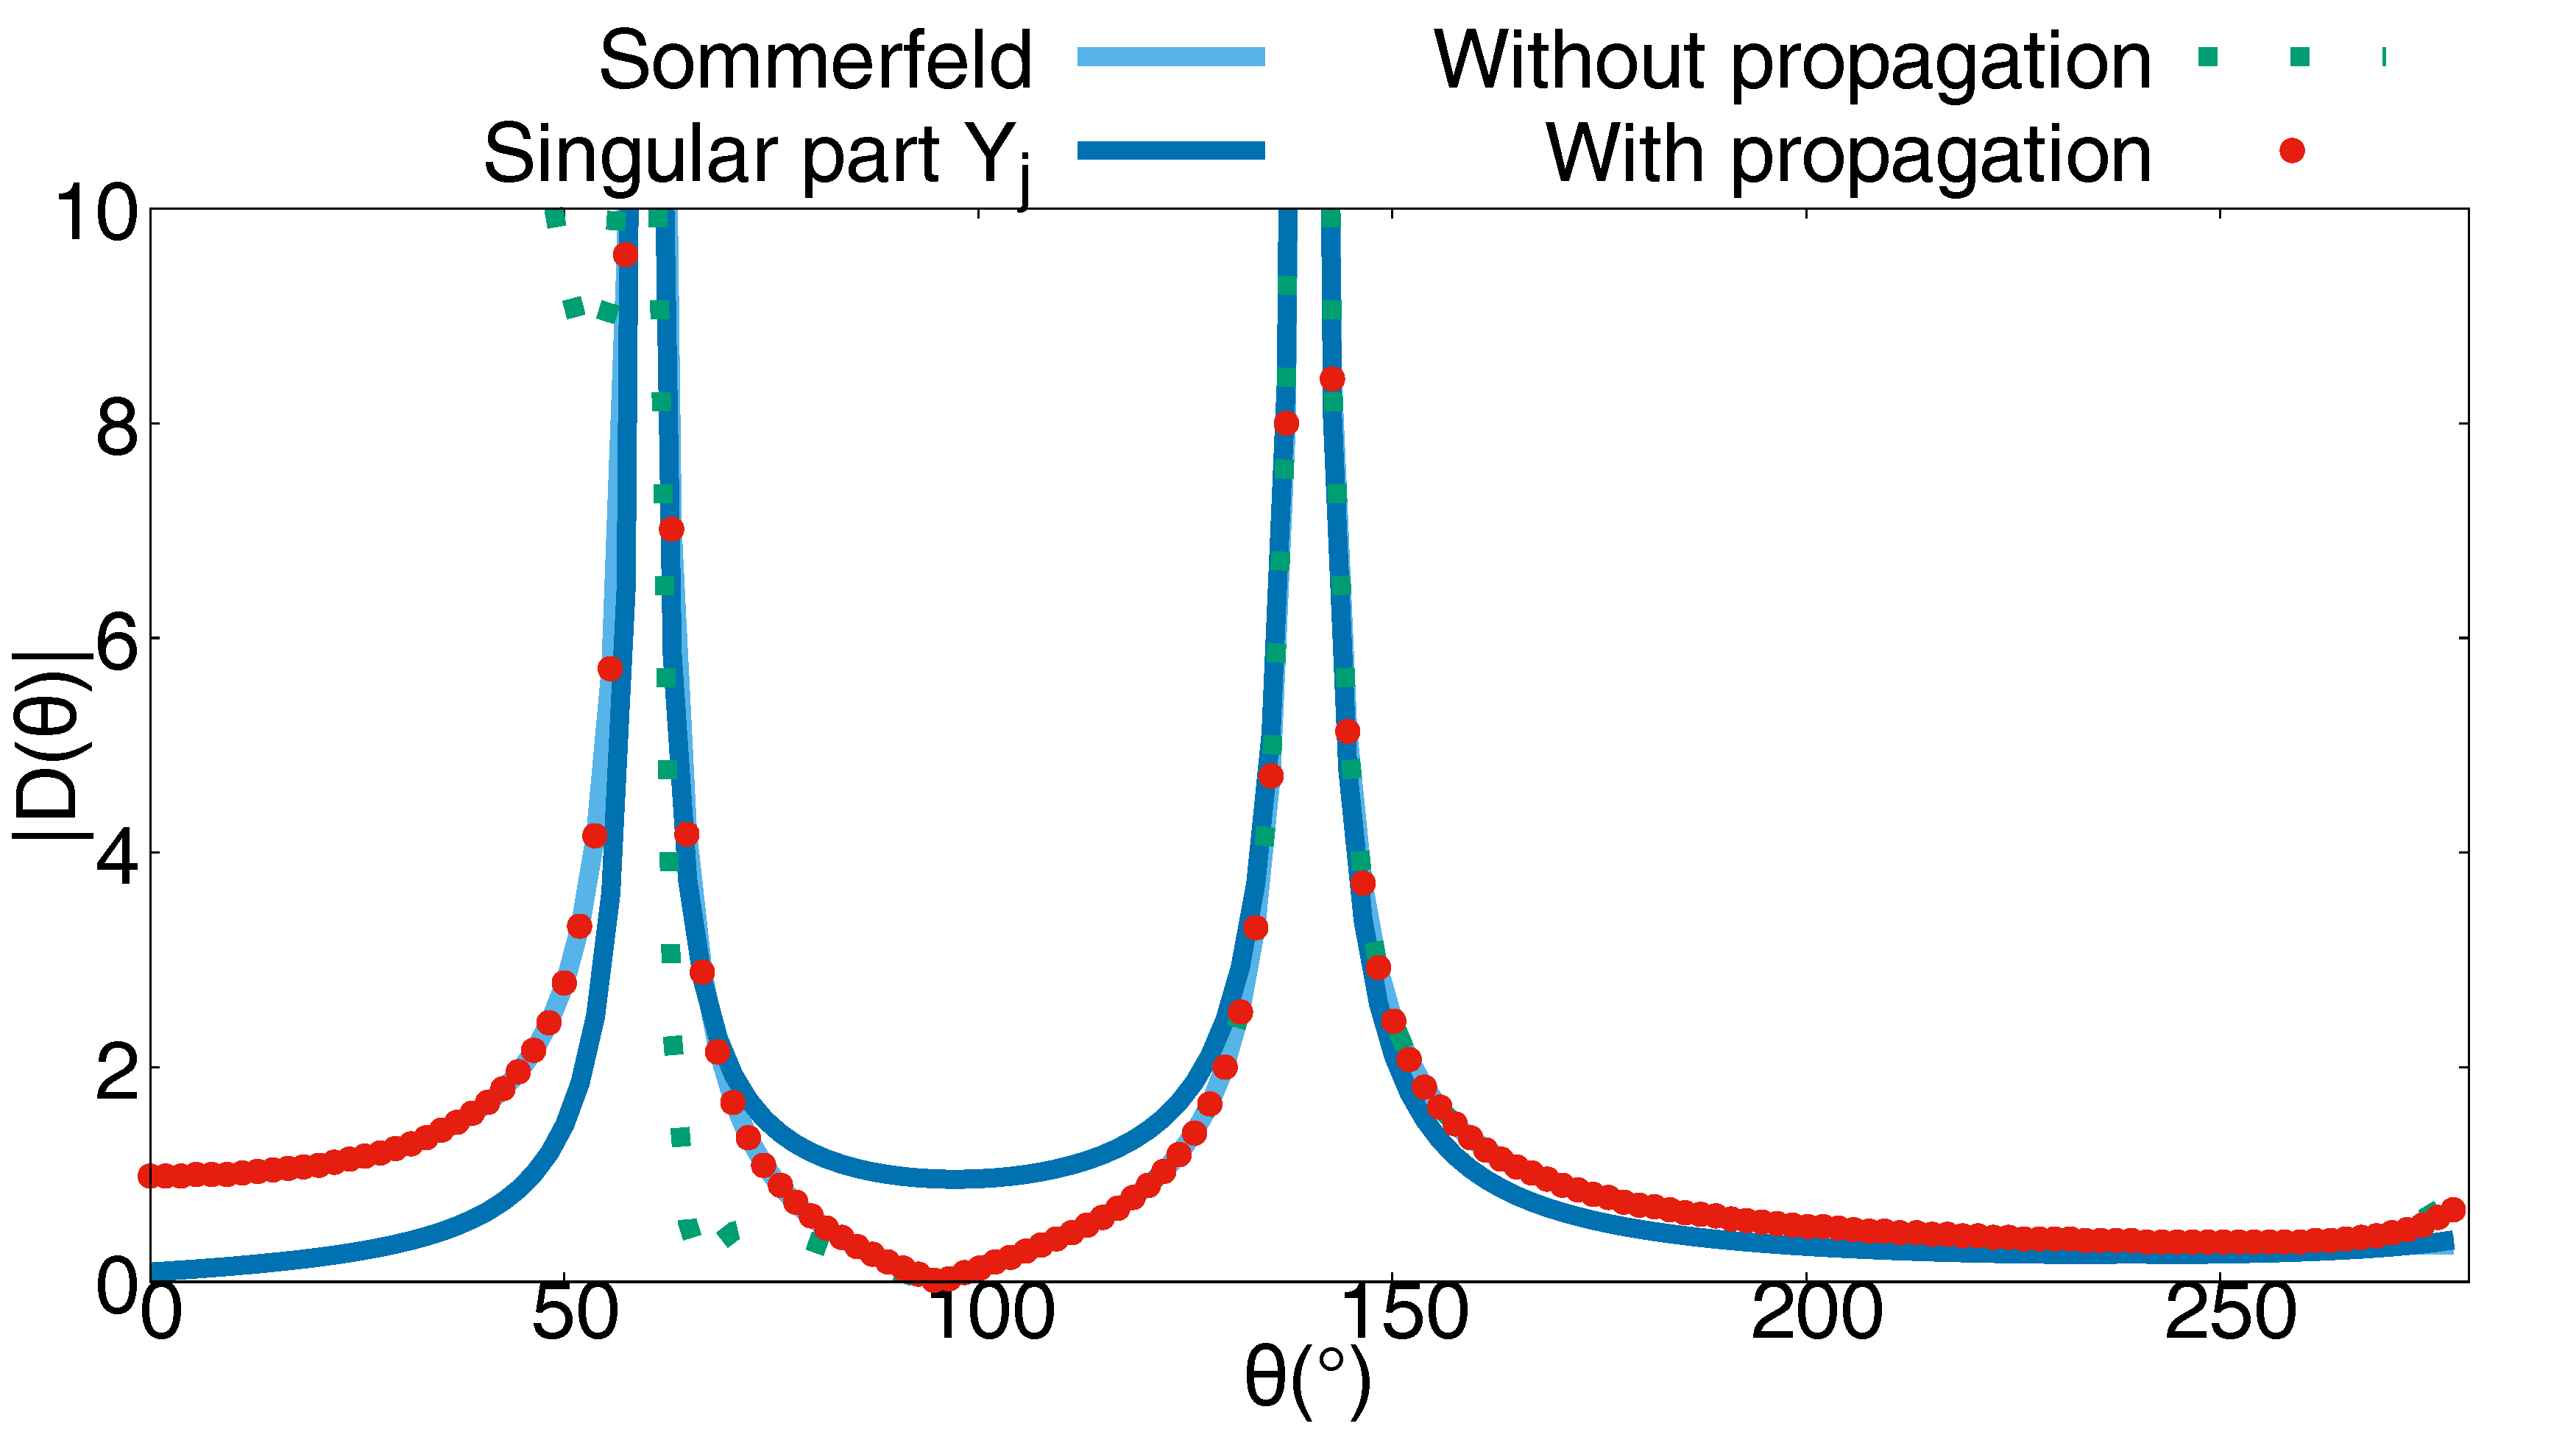
\includegraphics[width=\textwidth]{images/chapter2/Figure9c.pdf}
        \caption{$2\varphi = 280^o$, $\theta_{\rm inc} = 240^o$}
        \label{chapter5:figure13d}
    \end{subfigure}
\begin{subfigure}[b]{0.49\textwidth}
        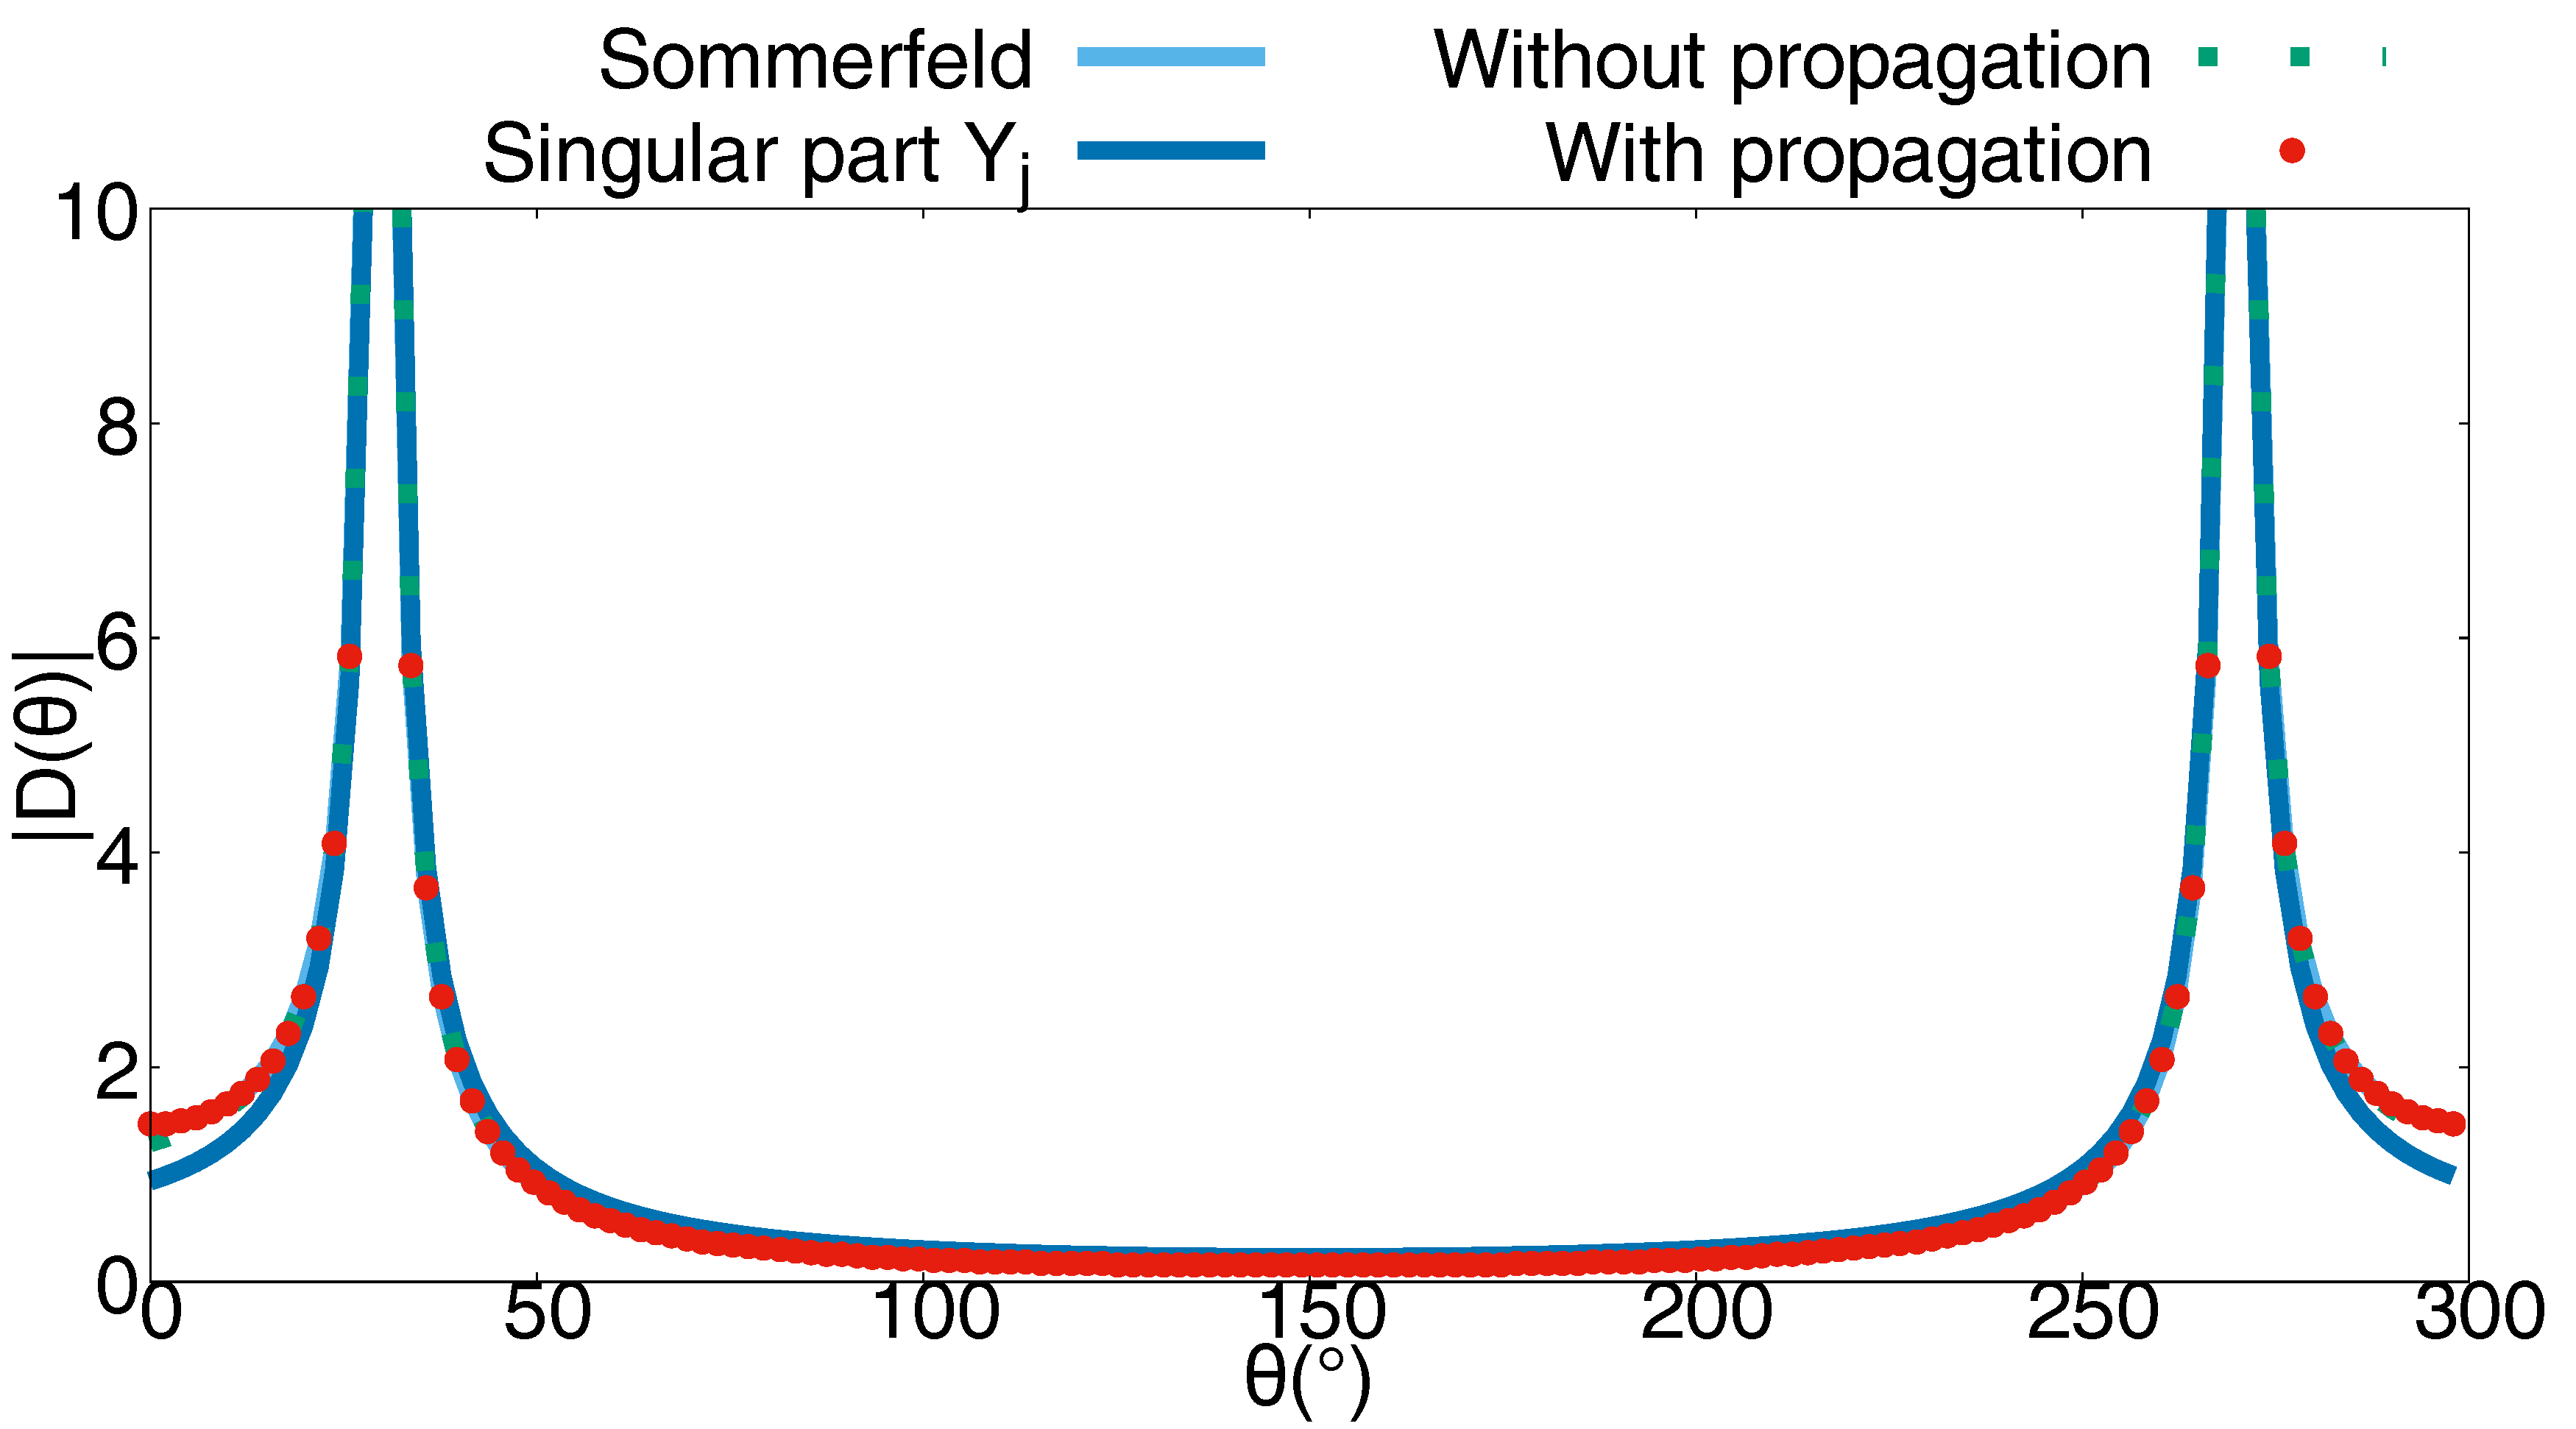
\includegraphics[width=\textwidth]{images/chapter2/Figure9d.pdf}
        \caption{$2\varphi = 300^o$, $\theta_{\rm inc} = 150^o$}
        \label{chapter5:figure13c}
    \end{subfigure}
\caption
[Diffraction  coefficient computed with the recursive formula of spectral functions and with the Sommerfeld method, in the case of Neumann boundary conditions]
{Diffraction  coefficient computed with the spectral functions and with the Sommerfeld method, in the case of Neumann boundary conditions.}
\label{chapter5:figure13}
\end{figure}


 In each of these figures, the continuous light blue line represents the modules of the diffraction coefficients obtained using the Sommerfeld integral method, the continuous dark blue line represents those obtained using the Spectral function singular part $Y_j$ alone, the short-dashed green line represents those obtained using the Spectral functions method without propagation of the solution and the red circles represent those obtained using the spectral functions method with propagation of the solution described in paragraph \ref{propag_sol}.

On Figs.~\ref{chapter5:figure12a},~\ref{chapter5:figure12b},~\ref{chapter5:figure13a} and ~\ref{chapter5:figure13b} the wedge angles are lower than $\pi$ and on figs.~\ref{chapter5:figure12c},~\ref{chapter5:figure12d},~\ref{chapter5:figure13c} and ~\ref{chapter5:figure13d} the wedge angles are greater than $\pi$. In all cases, it appears clearly that both the regular part of the solution and the recursive method are necessary to obtain optimal results. When both of these are included, diffraction coefficients obtained with Spectral functions are close to those of the Sommerfeld method. In addition, the run time to evaluate the diffraction coefficients in 250 different observation points, in each of the presented configurations, using an Intel(R) Xeon(R) CPU E3-1240 v3 is under 0.1 seconds for both methods. 

%
% Troisième chapitre
%\chapter[][2D Elastic Case]{The spectral functions method for 2D elastic wave diffraction by a stress-free wedge}
\label{chap-2D}

\section*{Introduction}
%The problem of plane wave diffraction by a wedge has been of great interest to researchers for over a century. The first to solve this type of problem in the case of an electromagnetic wave was Sommerfeld \cite{Sommerfeld}, who expressed the solution analytically, in the form of an integral called the Sommerfeld integral. At the same time, Macdonald \cite{Macdo} also expressed the solution to diffraction of a scalar plane wave analytically, as a series.

In the case of a plane elastic wave, it seems that the solution cannot be computed analytically. Therefore, semi-analytical resolutions and far-field ($kr>>1$, $k$ being the wave number and $r$ being the distance of observation) asymptotics have become common approaches. In this regard, the Geometrical Theory of Diffraction (GTD) was first introduced in electromagnetics by Keller \cite{GTD} and applied to elastodynamics by Achenbach et al. in 2D (when the incident wave vector is in the plane normal to the edge)  and in 3D \cite{Achenbach, GTDAchenbach}. The total asymptotic fields obtained with this method are spatially non-uniform in the sense that they diverge at shadow boundaries of the Geometrical Elastodynamics (GE) field. To solve this problem, some uniform corrections of the GTD have been developed. The Physical Theory of Diffraction (PTD) has been developed in electromagnetics by Ufimtsev \cite{Ufmi} and extended to elastic waves \cite{Zernov,PTDdarmon} but it is computationally expensive for large scatterers. Another uniform correction is the Uniform Asymptotic Theory (UAT) developed in elastodynamics by Achenbach et al. \cite{Achenbach}. This method has been tested by Fradkin and Stacey \cite{Fradkinelliptic}, using a finite difference algorithm. It requires an artificial extension of the scattering surface and the construction of fictitious rays \cite{Bouche}. For these reasons, a more commonly used uniform correction of the GTD method is the Uniform Theory of Diffraction (UTD). It was developed in electromagnetics by Kouyoumjian and Pathak \cite{Kouyoumjian} using the Pauli-Clemmow \cite{Pauli} asymptotic approximation of integrals. Kamta Djakou et al. \cite{Audrey} have extended it to elastodynamics with application to the scattering from a half-plane. This method is computationally efficient but still requires a trustworthy diffraction model in order to be applied. For the scalar case of 2D wedge diffraction of a shear horizontally polarized incident wave, a comparison of asymptotic (GTD and uniform) and exact solutions has been carried out in elastodynamics by Aristizabal et al. \cite{Aristizabal}.

The problem of acoustic diffraction in a system of wedge-shaped regions was studied by Klem-Musatov \cite{Klem-Musatov}, but this system is too complex to be solved in general cases. For the very general problem of acoustic wave propagation in a homogeneous or inhomogeneous medium delimited by an arbitrary-shaped boundary, a mathematical model has been rigorously presented by Aizenberg and Ayzenberg \cite{Aizenberg}. Ayzenberg \cite{Ayzenberg} shows how this model can be numerically applied to the case of wedge diffraction. However, it appears that parallel programming is necessary to obtain a short computation time.

Another method, in which the free-space Green's tensor is used to express the Fourier transform of the displacement on the edges, was first developed by Gautesen for the case of a longitudinal wave diffracted by an elastic quarter-space \cite{GautesenLwave} and extended to the case of a scattered Rayleigh wave for wedge angles in the range $\lbrack 63^o, 180^o \rbrack$ for wedge angles lower than $\pi$ \cite{GautesenRayleigh3,GautesenRayleigh} and to $\lbrack 189^o, 327^o \rbrack$ for wedge angles higher than $\pi$ \cite{GautesenRayleigh2}. This method has also been applied to horizontally polarized shear waves scattered by a wedge-shaped interface between two different elastic materials \cite{GautesenSHwave}. The problem of elastic wave diffraction by a wedge has also been tackled by Budaev \cite{Budaev,BudaevInclusion,BudaevBook} and reduced to a singular integral equation. However, no clear numerical scheme of resolution has been proposed. Budaev and Bogy \cite{Rayleigh} have applied this method to the case of an incident Rayleigh wave and have proposed a corresponding numerical resolution. However, the theoretical development was incomplete and has been clarified by Kamotski et al. \cite{KamotskiFradkin}. Budaev and Bogy's method, called the Sommerfeld Integral (SI) method, and Gautesen's method, called the Laplace Transform (LT) method have both been extended by Gautesen and Fradkin \cite{GautesenFradkin} to the case of an elastic wave diffracted by a stress-free wedge of angle lower than $\pi$. They offer a comparison of the two methods and an experimental validation is given by Chapman et al. \cite{ChapmanBurch}.

Another boundary integral approach was developed by Croisille and Lebeau \cite{CroisilleLebeau} in the case of an acoustic plane wave scattered by an immersed elastic wedge. This is called the spectral functions method and was described both theoretically and numerically for the case of an immersed wedge of angle lower than $\pi$ \cite{CroisilleLebeau}.  In the 2D case of an acoustic wave incident on a soft wedge, the method has been developed numerically by Chehade et al. \cite{article}. The spectral functions method was also used by Kamotski and Lebeau \cite{KamotskiLebeau} to prove existence and uniqueness of the solution to the 2D problem of a plane elastic wave diffracted by a stress free wedge of arbitrary angle. However, no numerical scheme of resolution was given. The aim of the current paper is to propose and implement the numerical aspects of the spectral functions method in the 2D case of a stress-free elastic wedge of any angle. The results are validated by comparison to Gautesen's LT code \cite{GautesenFradkin} for wedge angles lower than $\pi$ and to the spectral finite elements code of Imperiale et al. developed for the commercial software CIVA \cite{imperiale_ut_2016, imperiale_ut_2017} for wedge angles higher than $\pi$.

The structure of the paper is the following. The problem at hand is stated in section 2. Section 3 presents an integral formulation of the solution in terms of two unknown functions called the spectral functions. This formulation is then used to compute a far-field approximation of the displacement field, following the steps of Kamotski and Lebeau \cite{KamotskiLebeau}, using an unknown coefficient called the diffraction coefficient, expressed in terms of the spectral functions. In section 4, the semi-analytical computation of these spectral functions is presented in detail. The first part of this computation consists in determining the poles and residues of these functions thanks to an algorithm adapted from Croisille and Lebeau \cite{CroisilleLebeau}. The second step is to approximate the remaining regular part of the spectral functions, and the necessary computations are detailed here. The third and final step is called the "propagation of the solution". It is based on a system of recursive equations determined by Croisille and Lebeau \cite{CroisilleLebeau}, which has been modified in order to be applicable to our case, and the computations necessary to a numerical evaluation of these equations are given here. Finally, some numerical results and validation of diffraction coefficients are given in section 5. Appendices A and B give useful details for the numerical computation of certain parts of the spectral functions.
\section{Problem statement}
\begin{figure}[h]
\centering
\resizebox{!}{0.2\textheight}{
	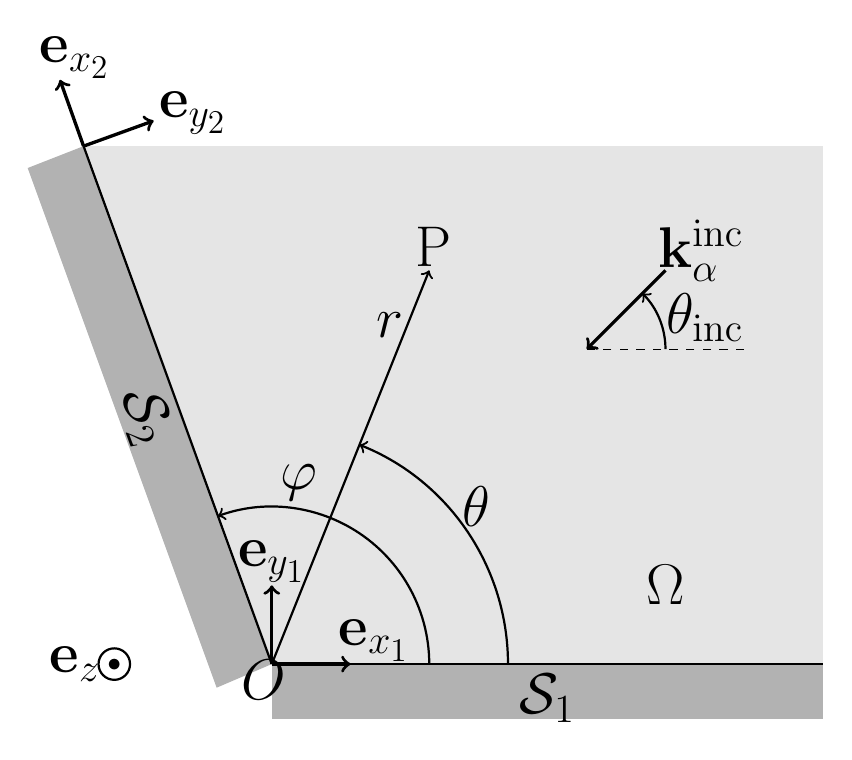
\begin{tikzpicture}
	\fill[color=gray!20] (0,0) -- (7,0)  -- (7,6.5778) -- (-2.39,6.5778) -- cycle;  
	\draw[ thick, ->] (2,0) arc (0:110:2);
	
	\fill[color=gray!60] (0,0) -- (7,0)  -- (7,-0.7) -- (0,-0.7) -- cycle;  
	
	\fill[color=gray!60] (0,0) --  (-2.39,6.5778) --(-3.1,6.3) -- (-0.7,-0.3) -- cycle; 
	
	
	\draw[thick, color = black]  (0,0) -- (7,0) node[midway,below] {\huge $\mathcal{S}_1$ };
	
	\draw[thick, color = black]  (0,0) -- (-2.39,6.5778) node[midway,below,sloped] { \huge $\mathcal{S}_2$};
	
	\draw[very thick, ->] (-2.39,6.5778) -- (-2.69,7.42);
	
	\node[scale=1] at (-2.5,7.7){ \huge $\mathbf{e}_{x_2}$};
	
	\draw[very thick, ->] (-2.39,6.5778) -- (-1.5,6.9);
	
	\node at (-1,7){\huge $\mathbf{e}_{y_2} $};
	
	
	\node at (0.35,2.3){\huge $\varphi$} ; 
	
	\draw[very thick, ->] (0,0) -- (1,0);
	
	\node at (1.3,0.3) {\huge $\mathbf{e}_{x_1} $};
	
	\draw[very thick, ->] (0,0) -- (0,1);
	
	\node at (0,1.3){\huge $\mathbf{e}_{y_1} $};
	
	\node at (-2,-0.01) {$\bullet$};
	
	\draw[thick] (-2,0) circle (0.2);
	
	\node at (-2.5,0){\huge $\mathbf{e}_{z}$};
	
	\draw[very thick, ->] (5,5) -- (4,4);
	
	\draw[dashed] (6,4) -- (4,4);
	
	\draw[thick, ->] (5,4) arc (0:45:1);
	
	\node at (5.5,4.4){\huge $\theta_{\rm inc}$};
	
	\node at (5.45,5.25){\huge $\mathbf{k}^{\rm inc}_{\alpha}$};
	
	\node at (-0.1,-0.2){\huge $O$};
	
	\node at (5,1){\huge $\Omega$ };
	
	\draw[thick, ->] (0,0) -- (2,5); 
	
	\draw[thick, ->] (3,0) arc (0:68.2:3);
	
	\node at (2.6,2){\huge $\theta$};
	
	\node at (1.5,4.3){\huge $r$};
	
	\node at (2.06,5.3){\huge P};
	
	\end{tikzpicture}
    }
	\caption{Plane wave incident on a stress-free wedge of angle $\varphi$ }
        \label{wedge}
\end{figure}
Let us consider the diffraction problem of a plane longitudinal elastic wave $\mathbf{u}^{inc}$ incident on a wedge delimited by the stress-free infinite plane faces $\mathcal{S}_1$ and $\mathcal{S}_2$. The inside of the wedge is a homogeneous isotropic medium occupying the space $\Omega$ defined by :
\begin{equation}
\Omega=\{ (r\cos \theta, r \sin \theta) \backslash \theta \in \rbrack 0, \varphi \lbrack \} 
\end{equation}
And the incident plane wave is of the form
\begin{equation}
\mathbf{u}^{inc}(\mathbf{x},t)=\mathbf{A}_{\alpha}e^{i(\mathbf{k}_{\alpha}^{inc}\cdot \mathbf{x}-\omega t)}
\end{equation}
$\alpha=L,T$ is the type of the incident plane wave (longitudinal or transversal), $\mathbf{A}_{\alpha}$ is the amplitude vector and $\mathbf{k}_{\alpha}^{inc}$ is the incident wave vector. The Cartesian coordinate system $(O; \mathbf{e}_{x_1}, \mathbf{e}_{y_1} )$ is linked to the face $\mathcal{S}_1$ of the wedge and $(O;  \mathbf{e}_{x_2}, \mathbf{e}_{y_2} )$ is linked to the face $\mathcal{S}_2$, as shown in Fig.~\ref{wedge}. These coordinate systems have the same origin located on the wedge edge which coincides with the $z$-axis. Let $\mathbf{x} = (x'_1,y'_1)_{ (\mathbf{e}_{x_1}, \mathbf{e}_{y_1}) } = (x'_2,y'_2)_{ (\mathbf{e}_{x_2}, \mathbf{e}_{y_2})}$ be a position vector $\mathbf{x} = (r,\theta)$ in a local basis of polar coordinates associated to the coordinates $(x'_1,y'_1)$. In the following, except when specified otherwise, all vectors are expressed in the coordinate system  $(O; \mathbf{e}_{x_1}, \mathbf{e}_{y_1} )$. The incident wave vector is given by 
\begin{equation}
\mathbf{k}_{\alpha}^{inc}=\frac{\omega}{c_{\alpha}} 
\begin{pmatrix}
\cos\theta_{inc} \\ 
\sin\theta_{inc} 
\end{pmatrix}
\end{equation}
$c_L=\sqrt{(\underline{\lambda}+2\underline{\mu})/\rho}$ is the velocity of the longitudinal waves,  $c_T=\sqrt{\underline{\mu}/\rho}$ is the velocity of the transversal ones and $\underline{\lambda}, \underline{\mu}$ are the Lam\'{e} coefficients. The amplitude vector may be colinear (in the case of a longitudinal wave) or normal (in the case of a transversal wave) to the incident wave vector. It will then be directed by $\mathbf{\hat{i}_L}$ or $\mathbf{\hat{i}_{T}}$ respectively :
\begin{equation}
\mathbf{\hat{i}_L} = \begin{pmatrix}
\cos\theta_{inc} \\ \sin\theta_{inc}
\end{pmatrix}
~~~~
\mathbf{\hat{i}_{T}} = \begin{pmatrix}
-\sin\theta_{inc} \\ \cos\theta_{inc}
\end{pmatrix}
\label{ivec}
\end{equation}
In all the following, bold characters are reserved for matrices in order to simplify notations and the time-harmonic factor $e^{-i\omega t}$ is omitted.

The unknown displacement field $u$ is a solution of the linear elasticity equations for a homogeneous isotropic medium and verifies stress-free boundary conditions on the wedge faces. Let us suppose that the total displacement field is the sum of an incident and a scattered field :
\begin{equation}
u=u_0+u^{inc}
\end{equation}
The dimensionless problem is obtained thanks to the following change in variables :
\begin{subequations}
\begin{equation}
x=\frac{\omega}{c_L} x', \hspace{1em} y=\frac{\omega}{c_L} y'
\end{equation}
\begin{equation}
u_0(x',y')=v(x,y)
\end{equation}
\label{adim}
\end{subequations}
The problem that we wish to solve is the following :

\begin{equation}
(\mathcal{P}^{\alpha}) \hspace{2em} \left\{~~
\begin{matrix}
(E+1)v=0 & (\Omega) \\
Bv=-B \rm v_{\alpha}^{inc} & (\mathcal{S})
\end{matrix}
\right.
\label{Padim}
\end{equation}
where $E$ and $B$ are respectively the elasticity and normal stress operators:
\begin{gather}
Ev=\mu \Delta v +(\lambda+\mu) \nabla \, \nabla v \label{defE}\\
Bv=(\lambda \nabla v .\mathbf{\mathbb{I}_2}+2\mu \mathbf{\varepsilon} (v)).n\label{defB}
\end{gather}
$\mathbb{I}_2$ is the two-dimensional identity matrix and $n$ is the inward normal to the faces of the wedge ($n=e_{y_j}$ on $\mathcal{S}_j$). The dimensionless Lam\'{e} coefficients are given by
\begin{equation}
\lambda=\frac{\underline{\lambda}}{\rho c_L^2}, \; \; \; \; \mu=\frac{\underline{\mu}}{\rho c_L^2}
\label{LameAdim}
\end{equation}
The deformations tensor is given by 
\begin{equation}
\varepsilon(v)=\dfrac{1}{2}\begin{pmatrix}
2\dfrac{\partial v_1}{\partial x} & \dfrac{\partial v_1}{\partial y}+\dfrac{\partial v_2}{\partial x} \\
\dfrac{\partial v_1}{\partial y}+\dfrac{\partial v_2}{\partial x}& 2\dfrac{\partial v_2}{\partial y}
\end{pmatrix}
\end{equation}
where $(v_1,v_2)$ are the components of vector $v$ and the dimensionless incident waves are
\begin{equation}
\rm v_L^{inc}(r,\theta)=\begin{pmatrix}
\cos \theta_{inc} \\
\sin \theta_{inc}
\end{pmatrix} e^{ir\nu_L \cos(\theta-\theta_{inc})}
\hspace{2em}
\rm v_T^{inc}(r,\theta)=\begin{pmatrix}
-\sin \theta_{inc} \\
\cos \theta_{inc}
\end{pmatrix} e^{ir\nu_T \cos(\theta-\theta_{inc})} 
\end{equation}
Finally, let us define the following ratios :
\begin{equation}
\nu_L=1 \hspace{2em} \nu_T=\frac{c_L}{c_T} \hspace{2em} \nu_R=\frac{c_L}{c_R} ,
\label{nuLnuT}
\end{equation}
where $c_R$ is the Rayleigh wave velocity.

\section{Integral Formulation of the solution}
The first step in solving problem $(\mathcal{P}^{\alpha})$ is to formulate the solution as an integral, following the formalism of Kamotski and Lebeau \cite{KamotskiLebeau}. In order to do so, a new class of functions is defined, as well as the outgoing solution of the problem. The main ideas of their development are reproduced here.
\subsection{Limiting absorption principle}
The limiting absorption principle is applied to $(\mathcal{P}^{\alpha})$, meaning that it is considered as a special case ($\varepsilon=0$ i.e. no medium absorption) of the problem
\begin{equation}
(\mathcal{P}^{\alpha}_{\varepsilon}) \hspace{2em} \left\{~~
\begin{matrix}
(E+e^{-2i\varepsilon})v^{\varepsilon}=0 & (\Omega) \\
Bv^{\varepsilon}=-B \rm v_{\alpha}^{inc} & (\mathcal{S})
\end{matrix}
\right.
\label{Pabs}
\end{equation}
Kamotski and Lebeau \cite{KamotskiLebeau} have shown that this problem admits a unique solution, which is the sum of two contributions, corresponding to each of the faces of the wedge
\begin{equation}
v^{\varepsilon}=v_1^{\varepsilon}+v_2^{\varepsilon},
\label{v1+v2}
\end{equation}
where functions $v_j^{\varepsilon}$ are defined in all of $\mathbb{R}^2$ by
\begin{equation}
v_j^{\varepsilon}=-(E+e^{-2i\varepsilon})^{-1} \begin{bmatrix}
\begin{pmatrix}
\alpha_j \\
\beta_j
\end{pmatrix}
\otimes \delta_{\mathcal{S}_j}
\end{bmatrix},
\label{vjdef}
\end{equation}
where $\delta_{\mathcal{S}_j}$ is the Dirac distribution associated to face $\mathcal{S}_j$. It is defined by its action on an arbitrary test function $f \in C_0^{\infty}(\mathbb{R}^2)$ :
\begin{equation}
\langle \delta_{\mathcal{S}_j},f\rangle=\int_0^{\infty}f((x_j,0)\, dx_j
\label{defDirac}
\end{equation}
The distributions $\alpha_j$ and $\beta_j$ are unknown and are supposed to belong to the special class $\mathcal{A}$ defined hereafter.
%\begin{mydef}
%We say that $f \in \mathcal{A}$ if $f \in \mathcal{S}'(\mathbb{R}), \mbox{supp} f \subset \mathbb{R}_+$ and
%\begin{gather}
% \exists C_0>0 \mbox{ such that } \underset{-\pi<\theta<0}{sup} \int_{C_0}^{+\infty}|\hat{f}(\rho e^{i\theta})|^2\,d\rho <+\infty \\
%\hat{f} \mbox{ is holomorphic in neighborhoods of } \nu_L, \nu_T, \nu_R.
%\end{gather}
% \label{defA}
%\end{mydef}
The notation $\hat{f}$ refers to the Fourier transform of the function $f$:
\begin{equation}
\hat{f}(\xi)=\int_{\mathbb{R}}e^{-ix\xi}f(x)\,dx
\label{defFouriersimple}
\end{equation}
and $\mathcal{S}'(\mathbb{R})$ is the space of tempered distributions on $\mathbb{R}$. Using this definition, Kamotski and Lebeau \cite{KamotskiLebeau} then obtain the following:
%\begin{lemme}
%Suppose $\alpha_j, \beta_j \in \mathcal{A}, j=1,2$. Then the two tempered distributions $v_j^{\varepsilon}$ defined by (\ref{vjdef}) converge in $\mathcal{S}'(\mathbb{R})$ when $\varepsilon \rightarrow 0$ towards two tempered distributions $v_j^0 \in \mathcal{S}'(\mathbb{R})$ which solve
%\begin{equation}
%(E+1)v_j^0=-
%\begin{pmatrix}
%\alpha_j \\
%\beta_j
%\end{pmatrix}
%\otimes \delta_{\mathcal{S}_j}
%\end{equation}
%Furthermore, the following properties are true for all $\varepsilon \in \lbrack 0,\pi \lbrack $:
%\begin{description}
%  \item[(i)] $v_j^{\varepsilon}$ are continuous in $\mathbb{R}^2$
%  \item[(ii)] in polar coordinates $(r,\theta)$, we have
%  \begin{gather}
% v_j^{\varepsilon} \in C(\lbrack 0,2\pi \rbrack; H^1_{loc}(\mathbb{R}_+))\\
% \frac{1}{r}\frac{\partial v_j^{\varepsilon}}{\partial \theta}\in C(\lbrack0,2\pi\rbrack;L^2_{loc}(\mathbb{R}_+))
%\end{gather}
%\end{description}
%\end{lemme}
%Finally, this lemma justifies the following definition
%\begin{mydef}
%We call $v$  an outgoing solution of  $(\mathcal{P}^{\alpha})$ if $v$ is a solution of the form
%\begin{equation}
%v=v_1+v_2,
%\end{equation}
%with
%\begin{equation}
%v_j=-\underset{\varepsilon\rightarrow0}{lim}(E+e^{-2i\varepsilon})^{-1} \begin{bmatrix}
%\begin{pmatrix}
%\alpha_j \\
%\beta_j
%\end{pmatrix}
%\otimes \delta_{\mathcal{S}_j}
%\end{bmatrix},
%\end{equation}
%where $\alpha_j,\beta_j \in\mathcal{A},j=1,2$.
%\end{mydef}
Existence and uniqueness of the outgoing solution was demonstrated by Kamotski and Lebeau \cite{KamotskiLebeau} and is not the object of this paper. Our goal is to propose a detailed method of numerical computation of this solution.

The limiting absorption principle presented above leads to a rigorous definition of the solution to the problem $(\mathcal{P}^{\alpha})$. It is also useful in order to derive an integral formulation of this solution.
\subsection{Integral formulation}
In order to compute the integral formulation of the solution, the two-sided Fourier transform of a tempered distribution and its inverse are defined in the following manner :
\begin{subequations}
\begin{equation}
\hat{f}(\xi,\eta)=\int \int_{\mathbb{R}^2}f(x,y)e^{-i(x\xi+y\eta)}\, {\rm d}x {\rm d}y
\label{fourierdef}
\end{equation}
\begin{equation}
f(x,y)=\frac{1}{4\pi^2}\int\int_{\mathbb{R}^2} \hat{f}(\xi,\eta)e^{i(x\xi+y\eta)}\rm d\xi \rm d\eta
\label{invfourierdef}
\end{equation}
\label{fullfourierdef}
\end{subequations}
The first step is to take the two-sided Fourier transform of equation \eqref{vjdef}. This is permitted since all the encountered distributions are tempered distributions (as discussed in the previous subsection).
\begin{equation}
\hat{v}^{\epsilon}_j(\xi,\eta)=(\mathbf{M}-e^{-2i\varepsilon}\mathbf{\mathbb{I}_2})^{-1}\Sigma_j(\xi),
\label{matMvjeps}
\end{equation}
where $\Sigma_j, \, j=1,2$  are two unknown functions called the spectral functions such that
\begin{equation}
\Sigma_j(\xi)=\begin{pmatrix}
\hat{\alpha_j}(\xi)\\ \hat{\beta_j}(\xi)
\end{pmatrix},
\end{equation}
and the matrix
\begin{equation}
\mathbf{M}=
\begin{pmatrix}
(\lambda+\mu)\xi^2+\mu(\xi^2+\eta^2) & (\lambda+\mu)\xi \eta \\
 (\lambda+\mu)\xi \eta & (\lambda+\mu)\eta^2+\mu(\xi^2+\eta^2)
\end{pmatrix}
\label{matM}
\end{equation}
is the two-sided Fourier transform of the elasticity operator $E$ defined by \eqref{defE}. By using the fact that $\lambda+2\mu=1$ and $\mu=1/\nu_T^2$ and by substituting \eqref{matM} into \eqref{matMvjeps}, functions $\hat{v}^{\epsilon}_j$ can be expressed as:
\begin{equation}
\hat{v}^{\varepsilon}_j(\xi,\eta)=\begin{pmatrix}
a(\xi,\eta) & b(\xi,\eta) \\
b(\xi,\eta) & a(\eta,\xi)
\end{pmatrix} \Sigma_j(\xi),
\end{equation}
where
\begin{subequations}
\begin{equation}
a(\xi,\eta)=\frac{\xi^2+\nu_T^2 \eta^2-\nu_T^2e^{-2i\varepsilon}}{(\xi^2+\eta^2-e^{-2i\varepsilon})(\xi^2+\eta^2-\nu_T^2e^{-2i\varepsilon})}
\end{equation}
\begin{equation}
b(\xi,\eta)=\frac{(1-\nu_T^2)\xi \eta}{(\xi^2+\eta^2-e^{-2i\varepsilon})(\xi^2+\eta^2-\nu_T^2e^{-2i\varepsilon})}
\end{equation}
\end{subequations}
The two-sided Fourier transform of $v_j^{\varepsilon}$ can now be reversed
\begin{equation}
v_j^{\varepsilon}(x_j,y_j)=\frac{1}{4\pi^2}\int_{- \infty}^{+ \infty} e^{ix_j\xi} \int_{-\infty}^{+\infty}e^{iy_j\eta}\begin{pmatrix}
a(\xi,\eta) & b(\xi,\eta) \\
b(\xi,\eta) & a(\eta,\xi)
\end{pmatrix} \,d\eta\, \Sigma_j(\xi) \,d\xi
 \label{invdouble}
\end{equation}
The inner integral is computed using Gauss' residue theorem. The poles of the integrand are $\eta=\pm \zeta_*^{\varepsilon}(\xi), *=L,T$, with
\begin{equation}
\zeta_*^{\varepsilon}(\xi)=\sqrt{e^{-2i\varepsilon}\nu_*^2-\xi^2}
\label{defzetaeps}
\end{equation}
thus yielding:
\begin{equation}
v_j^{\varepsilon}(x_j,y_j)=\frac{i}{4\pi}e^{2i\varepsilon}\int_{-\infty}^{+\infty} e^{ix_j\xi}\sum_{*=L,T}e^{i|y_j|\zeta_*^{\varepsilon}(\xi)}M_*^{\varepsilon}(\xi,\mbox{sgn }y_j)\Sigma_j(\xi)\,d\xi,
\label{vjeps}
\end{equation}
where, noting $t=\mbox{sgn }y_j$
\begin{equation}
\mathbf{M_L^{\varepsilon}}(\xi,t)=\begin{pmatrix}
\frac{\xi^2}{\zeta_L^{\varepsilon}(\xi)} &t\xi \\
t\xi & \zeta_L^{\varepsilon}(\xi)
\end{pmatrix}
~~\mbox{  and  }~~
\mathbf{M_T^{\varepsilon}}(\xi,t)=\begin{pmatrix}
\zeta_T^{\varepsilon}(\xi) & -t\xi \\
-t\xi & \frac{\xi^2}{\zeta_T^{\varepsilon}(\xi)}
\end{pmatrix}
\label{M*eps}
\end{equation}
According to Croisille and Lebeau \cite{CroisilleLebeau}, after slightly deforming the integration contour from $\mathbb{R}$ to $\Gamma_0$ represented in Fig. \ref{gamma0} integral \eqref{vjeps} converges when $\varepsilon \rightarrow 0$: 
\begin{equation}
v_j(x_j,y_j)=\frac{i}{4\pi}\int_{\Gamma_0} e^{ix_j\xi}\sum_{*=L,T}e^{i|y_j|\zeta_*(\xi)}\mathbf{M_*}(\xi,\mbox{sgn }y_j)\Sigma_j(\xi)\,d\xi
\label{vj0}
\end{equation}
In order to simplify notations, the exponent $\epsilon=0$ has been omitted.
The function $\zeta_*$ defined by taking $\epsilon=0$ in \eqref{defzetaeps} has multiple branch cuts. In order to satisfy the radiation condition at infinity
\begin{equation}
\lim\limits_{|y_j| \rightarrow +\infty} |v_j^{\varepsilon}(x_j,y_j)|=0,
\label{CR}
\end{equation}
we chose Im $\zeta_*(\xi)>0$ :
\begin{equation}
\zeta_*(\xi)=
\left\{
\begin{matrix}
i\sqrt{\xi^2-\nu_*^2}& \mbox{for } |\xi| \geq \nu_* \\
-\sqrt{\nu_*^2-\xi^2}& \mbox{for } |\xi| \leq \nu_*
\end{matrix}
\right.
\label{defzeta}
\end{equation}

The integral formulation \eqref{vj0} is an expression of the solution in terms of an unknown function $\Sigma_j$ called the spectral function. In the next section, by computing a far-field asymptotic approximation of this integral, we define a function of the observation angle $\theta$ (see Fig. \ref{wedge}) called the diffraction coefficient and express this coefficient in terms of $\Sigma_1$ and $\Sigma_2$.

\begin{figure}[h]
\centering
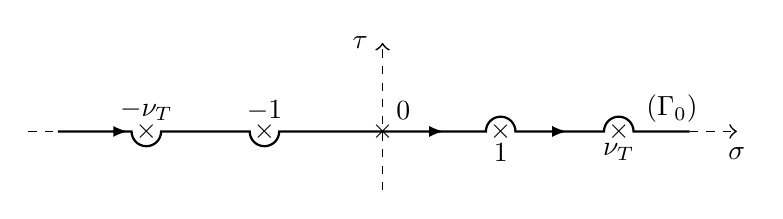
\begin{tikzpicture}[scale=0.75]
\node at (0,0) {$\times$};
\node at (0.35,0.35) {$0$};
\node at (2,0) {$\times$}; % Pole
\node at (4,0) {$\times$}; %pole
\node at (2,-0.35) {$1$};
\node at (4,-0.35) {$\nu_T$};
\node at (-2,0) {$\times$};
\node at (-4,0) {$\times$};
\node at (-2,0.35) {$-1$}; %pole
\node at (-4,0.35) {$-\nu_T$}; %pole
\node at (4.9,0.38) {$(\Gamma_0)$};
\node at (6,-0.38) {$\sigma$};
\node at (-0.38,1.5){$\tau$};

\draw[dashed,yshift=0pt]
(-6,0)--(-5.5,0);

\draw[dashed, yshift=0pt,decoration={ markings,  mark=at position 1 with {\arrow[scale=1.5]{>}}},
      postaction={decorate}]
(5.2,0)--(6.0,0);

\draw[dashed, yshift=0pt,decoration={ markings,  mark=at position 1 with {\arrow[scale=1.5]{>}}},
      postaction={decorate}]
      (0,-1)--(0,1.5);

\draw[thick,black,yshift=0pt,
decoration={ markings,  % This schema allows for fine-tuning the positions of arrows 
      mark=at position 0.1 with {\arrow{latex}},
      mark=at position 0.6 with {\arrow{latex}},
      mark=at position 0.8 with {\arrow{latex}}},
      postaction={decorate}]
      (-5.5,0) -- (-4.25,0)  arc (-180:0:0.25) -- (-2.25,0)  arc (-180:0:0.25)  -- (1.75,0)arc (180:0:0.25)  -- (3.75,0)arc (180:0:0.25) -- (5.2,0); % ca c'est l'axe
\end{tikzpicture}
\caption{Integration contour $\Gamma_0$ in the complex plane $\xi=\sigma+i\tau$.}
\label{gamma0}
\end{figure}

\subsection{Far-field asymptotics}
\label{farfield}
Let $P=(x',y')=(r\cos\theta,r\sin\theta)$ be an observation point, represented in Fig. \ref{wedge}. According to equation \eqref{adim}, the diffracted field at P is given by:
\begin{equation}
u_0(x',y')=v(\frac{\omega}{c_L}r\cos\theta,\frac{\omega}{c_L}r\sin\theta)
\end{equation}
Let $R=\frac{\omega r}{c_L}$ denote the far-field parameter. Our goal is to determine an asymptotic evaluation of the diffracted field when $R\rightarrow +\infty$. To do so, we begin by applying the following change of variables in integral \eqref{vj0} :
\begin{equation}
\begin{split}
 \xi&=\nu_*\cos\lambda \\
 d\xi&=-\nu_*\sin\lambda\, d\lambda,
\end{split}
\label{changevar2}
\end{equation}
yielding, in polar coordinates
\begin{equation}
v_1(r\cos\theta,r\sin\theta)=\frac{i}{4\pi} \int_{C_0}\sum_{*=L,T}\nu_*^2 e^{i\nu_*r\cos(\lambda+\bar{\theta})}\mathbf{ P_*}(\lambda,t)\Sigma_1(\nu_*\cos\lambda) \, d \lambda,
\label{v1pol}
\end{equation}
where $t=\rm sgn \sin \theta$,
\begin{equation}
\bar{\theta}=\left\{
\begin{matrix}
\theta & \rm if \theta \leq \pi \\
2\pi-\theta & \rm if \theta>\pi
\end{matrix}
\right. ,
\label{C3:thetatilde}
\end{equation}
contour $C_0$ is represented in Fig. \ref{steepestcontour} and
\begin{gather}
\mathbf{P_L}(\lambda,t)=
\begin{pmatrix}
\cos^2\lambda & -t\cos\lambda\sin\lambda \\
-t\cos\beta\sin\lambda & \sin^2\lambda
\end{pmatrix}\\
\mathbf{P_T}(\lambda)=\mathbf{\mathbb{I}_2}-\mathbf{P_L}(\lambda)
\end{gather}
Note that $\mathbf{P_*}(\lambda,-1)=\mathbf{P_*}(-\lambda,1)$. In the following, we will use the notation $\mathbf{P_*}(\lambda)=\mathbf{P_*}(\lambda,1)$.

An asymptotic evaluation of \eqref{v1pol} is determined using the steepest descent method. This consists of deforming integration contour $C_0$ into $\gamma_{\bar{\theta}}$ represented in Fig. \ref{steepestcontour}. The approximation is then the sum of two contributions:
\begin{equation}
v_1=v_1^{sing}+v_1^{diff},
\end{equation}
where $v_1^{sing}$ is the contribution of all the singularities of the spectral function $\Sigma_1$ crossed by the contour deformation and $v_1^{diff}$ is the contribution of the phase function's saddle point $\lambda_s=\pi-\bar{\theta}$, corresponding to the field diffracted by the wedge edge. We will see that the singularities crossed are either simple poles (corresponding to the reflected waves on the wedge faces or to the Rayleigh surface waves) or branch points (corresponding to head waves). In this paper, we are only concerned with the determination of the edge-diffracted field, which corresponds to the contribution of the saddle-point and is given by:
\begin{equation}
v_1^{diff}(r\cos\theta,r\sin\theta)=\frac{e^{-i\pi/4}}{2\sqrt{2\pi}}\sum_{*=L,T}\nu_*^2\frac{e^{-i\nu_*r}}{\sqrt{\nu_*r}}\mathbf{P_*}(\pi-\theta)\Sigma_1(-\nu_*\cos\theta)
\label{v1diff}
\end{equation}
Note that asymptotic evaluation \eqref{v1diff} is only valid when the saddle point $\lambda_s$ does not coincide with a singular point (pole or branch point) of the spectral function $\Sigma_1$. The poles of the spectral functions will be determined analytically in section \ref{singpart}. The branch points of the spectral functions are located at $\xi=\pm \nu_L$ and $\xi = \pm \nu_T$. Applying \eqref{changevar2}, this means that :
\begin{subequations}
\begin{equation}
\nu_*\cos\lambda_s=-\nu_*\cos\theta=\pm \nu_L=\pm 1
\label{eqbranch1}
\end{equation}
\begin{equation}
\rm or \hspace{1em} \nu_*\cos\lambda_s=-\nu_*\cos\theta=\pm \nu_T
\label{eqbranch2}
\end{equation}
\label{eqbranch}
\end{subequations}
For $*=L$, \eqref{eqbranch1} yields $\theta=0$ or $\theta=\pi$, meaning that the direction of observation is along the wedge's horizontal face $\mathcal{S}_1$. \eqref{eqbranch2} does not have a solution for $*=L$. For $*=T$, \eqref{eqbranch1} yields $\theta=\theta_c=\rm acos(1/\nu_T)$ or $\theta=\pi- \theta_c$, $\theta_c$ is called the critical angle, and \eqref{eqbranch2} yields $\theta=0$ or $\theta=\pi$. Borovikov \cite{Borovikov} gives some clues as to how to treat the case where the stationary phase point coincides with another singularity of the integrand. In this paper, it is assumed that $\lambda_s$ does not coalesce with a singularity of the integrand.

Similar considerations yield:
\begin{equation}
v_2^{diff}(x_2,y_2)=\frac{e^{-i\pi/4}}{2\sqrt{2\pi}}\sum_{*=L,T}\nu_*^2\frac{e^{-i\nu_*r}}{\sqrt{\nu_*r}}\mathbf{P_*}(\pi-(\varphi-\theta))\Sigma_2(-\nu_*\cos(\varphi-\theta))
\label{v2diff}
\end{equation}
The branch points are now located at $\bar{\theta}=\varphi$, $\bar{\theta}=\pi-\varphi$, $\bar{\theta}=\varphi-\theta_c$ and $\bar{\theta}=\pi-(\varphi-\theta_c)$.
The total diffracted field is the sum of the saddle-point contributions from each face
\begin{equation}
v^{diff}=v_1^{diff}+v_2^{diff}
\label{vdiff12}
\end{equation}
This can be identified with the total diffracted field written in terms of longitudinal and transversal contributions, 
\begin{equation}
v^{diff}=v^{diff}_L \hat{i}_L+v^{diff}_T \hat{i}_T,
\label{vdiffLT}
\end{equation}
with $\hat{i}_*$ defined by \eqref{ivec}, leading to the following definition of the diffraction coefficient $D_{\beta}^{\alpha}$ : 
\begin{equation}
v_{\beta}^{diff}(r\cos\theta,r\sin\theta)=D_{\beta}^{\alpha}(\theta)\frac{e^{-i\nu_{\beta}r}}{\sqrt{\nu_{\beta}r}} \rm v^{\alpha}_{inc}(r\cos\theta,r\sin\theta),
\label{defcoeffdiff}
\end{equation}
where $\beta=L,T$ is the type of the diffracted wave. The diffracted field is thus represented by a cylindrical wave, proportional to the incident wave and weighted by the diffraction coefficient. By substituting \eqref{v1diff}-\eqref{v2diff} into \eqref{vdiff12} and \eqref{defcoeffdiff} into \eqref{vdiffLT} and identifying the results, we finally obtain the expression of the diffraction coefficients in terms of the components $(\hat{\alpha}_j,\hat{\beta}_j), \, \, j=1,2$ of the spectral functions
\begin{gather}
\begin{split}
 D^{\alpha}_L(\theta)=\frac{e^{-i\pi/4}}{2\sqrt{2\pi}}&\big(\hat{\alpha}_1(-\cos\theta)\cos\theta+\hat{\beta}_1(-\cos\theta)\sin\theta\\
&+\hat{\alpha}_2(-\cos(\varphi-\theta))\cos(\varphi-\theta)+\hat{\beta}_2(-\cos(\varphi-\theta))\sin(\varphi-\theta)\big)
\end{split} \label{DL}\\
\begin{split}
 D^{\alpha}_T(\theta)=\nu_T^2\frac{e^{-i\pi/4}}{2\sqrt{2\pi}}&\big(-\hat{\alpha}_1(-\nu_T\cos\theta)\sin\theta+\hat{\beta}_1(-\nu_T\cos\theta)\cos\theta\\
&+\hat{\alpha}_2(-\nu_T\cos(\varphi-\theta))\sin(\varphi-\theta)-\hat{\beta}_2(-\nu_T\cos(\varphi-\theta))\cos(\varphi-\theta)\big) 
\end{split} \label{DT}
\end{gather}

\begin{figure}
\centering
\resizebox{!}{0.2\textheight}{
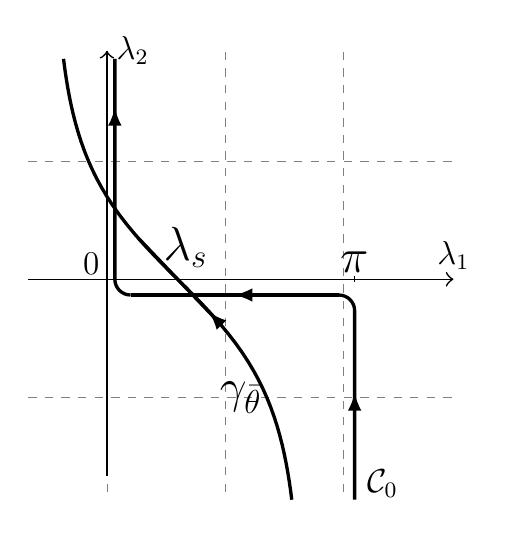
\begin{tikzpicture}
\draw[step=1.5cm,gray,very thin,dashed](-1,-2.7)grid(4.4,2.9);
%\draw[thin](-1,0)-- (0,0);
\draw[thin,decoration={ markings, mark=at position 1 with {\arrow[scale=1.5]{>}}},
      postaction={decorate}] (-1,0)  -- (4.4,0) node[above]{\large $\lambda_1$};
%\drawn[thin] -- (pi+1,0) node[below]{$\sigma$};
\draw[thin,decoration={ markings, mark=at position 1 with {\arrow[scale=1.5]{>}}},
      postaction={decorate}](0,-2.5)--(0,2.9) node[right]{\large $\lambda_2$};
\foreach \x in {pi} {  
  \draw (\x,-1pt) -- (\x,1pt) node[pos=0,above] {\LARGE $\pi$};
  }

\node at (-0.2,0.2) {\large $0$};
\node at (1,0.4) {\LARGE $\lambda_s$};
%\node at (3.5,-3.8) {$(\mathcal{C}_\xi)$};
\node at (3.5,-2.6) {\large $\mathcal{C}_0$};
\node at (1.7,-1.5) {\LARGE $\gamma_{\bar{\theta}}$};

\draw[black,very thick][domain=0:2.8] plot({2*pi/7 - acos(1/cosh(\x))*pi/180},\x);
\draw[black,very thick][domain=-2.8:0] plot({2*pi/7 + acos(1/cosh(\x))*pi/180},\x);
\draw[very thick,black,xshift=0pt,
decoration={ markings,  % This schema allows for fine-tuning the positions of arrows 
      mark=at position 0.8 with {\arrow{latex}}},
      postaction={decorate}]
      (0.3,-0.2) arc (270:180:0.2) -- (0.1,2.8); 
\draw[very thick,black,yshift=0pt,
decoration={ markings,  % This schema allows for fine-tuning the positions of arrows 
      mark=at position 0.5 with {\arrow{latex}}},
      postaction={decorate}]
      (pi-0.2,-0.2) -- (0.3,-0.2) ;
%\draw[very thick] (0.3,0) arc (270:180:0.2);

\draw[very thick,black,xshift=89.5pt,
decoration={ markings,  % This schema allows for fine-tuning the positions of arrows 
      mark=at position 0.5 with {\arrow{latex}}},
      postaction={decorate}]
      (0,-2.8) -- (0,-0.4) arc (0:90:0.2) ;
      \draw[very thick,black,
decoration={ markings,  % This schema allows for fine-tuning the positions of arrows 
      mark=at position 0.1 with {\arrow{latex}}},
      postaction={decorate}]
      (1.3988,-pi/6)  -- (0.3964,pi/6);  
\end{tikzpicture}
}
\caption{Integration contours $C_0$ and $\gamma_{\bar{\theta}}$ in the complex plane $\lambda=\lambda_1+i\lambda_2$. $\lambda_s$ is the stationary phase point.}
\label{steepestcontour}
\end{figure}

In order to determine the field diffracted by a wedge illuminated by an incident plane wave, it is sufficient to compute the diffraction coefficient. This coefficient has been expressed in terms of two unknown functions called the spectral functions. The semi-analytical computation of these functions is presented in the following section

\section{Semi-analytical evaluation of the spectral functions}
\label{section4}
The first step in computing the spectral functions is to determine a system of functional equations of which they are a solution. We will then show that these functions can be decomposed into two parts : a singular function, computed analytically, and a regular function, approached numerically.
\subsection{Functional equations}
In the previous section, the diffracted wave has been expressed in terms of two unknown functions called the spectral functions. In this subsection, a system of functional equations satisfied by these functions is determined.

The system of functional equations is determined using the boundary conditions on the faces of the wedge \eqref{Padim}. These can be expressed separately for each face of the wedge, using decomposition \eqref{v1+v2}:
\begin{equation}
\left\{
\begin{matrix}
B \big( v_1(x_1,0)+v_2(x_2 \cos \varphi, x_2 \sin \varphi) \big) = -B \rm v_{\alpha}^{inc}|_{\mathcal{S}_1} \\
B \big( v_2(x_2,0)+v_1(x_1 \cos \varphi, x_1 \sin \varphi) \big) = -B \rm v_{\alpha}^{inc}|_{\mathcal{S}_2}
\end{matrix}
\right.
\label{Bivi}
\end{equation}
Let us note  $(v_j^1,v_j^2),\, j=1,2$ the coordinates of vector $v_j$ in the Cartesian coordinate system $(x_j,y_j)$, represented in Fig.~\ref{wedge}.
By expliciting the normal stress operator \eqref{defB} in each of these systems,  system (\ref{Bivi}) can be expressed as
\begin{equation}
\left\{
\begin{array}{l}
B_1(v_1)+B_2(v_2)=-B\rm v_*^{inc}|_{\mathcal{S}_1} \\
B_1(v_2)+B_2(v_1)=-B\rm v_*^{inc}|_{\mathcal{S}_2}
\end{array}
\right.,
\end{equation}
where two new operators are defined:
\begin{gather}
B_1(v_1)=
\begin{pmatrix}
\mu \left( \frac{\partial v_1^1}{\partial y_1}+\frac{\partial v_1^2}{\partial x_1} \right) \\
~\\
\frac{\partial v_1^2}{\partial y_1}+\lambda \frac{\partial v_1^1}{\partial x_1}
\end{pmatrix} \label{B1v1expl}\\
B_2(v_2)=
\begin{pmatrix}
\mu \sin(2\varphi)\left( \frac{\partial v_2^1}{\partial x_2}-\frac{\partial v_2^2}{\partial y_2}\right)-\mu \cos(2\varphi)  \left( \frac{\partial v_2^1}{\partial y_2}+\frac{\partial v_2^2}{\partial x_2} \right)\\
~\\
(\lambda+2\mu \sin^2\varphi) \frac{\partial v_2^1}{\partial x_2}+(\lambda+2\mu \cos^2 \varphi)\frac{\partial v_2^2}{\partial y_2}-\mu \sin(2\varphi)  \left( \frac{\partial v_2^1}{\partial y_2}+\frac{\partial v_2^2}{\partial x_2} \right)
\end{pmatrix}\label{B2v2expl}
\end{gather}

The functional equations satisfied by the spectral functions are obtained by taking the Fourier transform of this system. 

The partial derivatives of $v_1$ with respect to $x_1$ and $y_1$ are evaluated in  $y_1=0, x_1 \geq 0$ using \eqref{vj0} before being substituted into \eqref{B1v1expl}. Finally, by using the following formula
$$\int_0^{+\infty} e^{-ix(\xi-\zeta)}\,dx=\frac{1}{i(\xi-\zeta)}, \; \mbox{ Im}\xi <0, \;  \mbox{ Im} \zeta>0, $$
the Fourier transform of operator $B_1$ is obtained :
\begin{equation}
\begin{split}
\int_0^{+\infty} e^{-ix\xi}B_1(v_1)(x)\,dx&=\frac{1}{2}\textbf{DM}(\Sigma_1)(\xi) \\
&=\frac{1}{2} \int_{\Gamma_0}\textbf{DM}(\xi,\zeta)\Sigma_1(\zeta)\,d\zeta
\end{split},
\label{B1DM}
\end{equation}
with
\begin{equation}
\textbf{DM}(\xi,\zeta)=\frac{1}{2i\pi} \frac{1}{\xi-\zeta} \textbf{dm}(\zeta) =\frac{1}{2i\pi} \frac{1}{\xi-\zeta} \begin{pmatrix}
-1 & A(\zeta) \\
B(\zeta) & -1
\end{pmatrix}
\label{defDM}
\end{equation}
and
\begin{equation}
A(\zeta)=\frac{z}{\zeta_T(z)}(1-2\mu Q(\zeta)) \hspace{3em} B(\zeta)=-\frac{\zeta}{\zeta_L(\zeta)}(1-2\mu Q(\zeta)) \hspace{3em}
Q(\zeta)=\zeta_L(\zeta) \zeta_T(\zeta)+\zeta^2,
\end{equation}
where $\zeta_*,\, *=L,T$ is given by \eqref{defzeta}.


The Fourier transform of operator $B_2$ is obtained  through a similar process. The partial derivatives of $v_2$ are evaluated in $x_2=x\cos\varphi,y_2=x\sin\varphi,x\geq0$ and then substituted into \eqref{B2v2expl} before applying the Fourier transform to the results. Finally, by using the following formula
\begin{equation}
\int_0^{+\infty} e^{-ix(\xi-(\zeta \cos \varphi + \zeta_*(\xi) \sin\phiti))}\,dx=\frac{1}{i(\xi-(\zeta \cos \varphi + \zeta_*(\xi)| \sin \varphi|)}, \; \mbox{ Im}\xi <0, \;  \mbox{ Im} \zeta>0 
\end{equation}
and by noting
\begin{equation}
D_*(\xi,\zeta)=\frac{1}{\xi-(\zeta \cos \varphi + \zeta_*(\zeta) \sin\phiti)}
\end{equation}
the Fourier transform of $B_2$ is obtained :
\begin{equation}
\int_0^{+\infty} e^{-ix\xi}B_2(v_2)(x)\,dx=\frac{1}{2}\textbf{TM}(\Sigma_2)(\xi) =\frac{1}{2} \int_{\Gamma_0}\textbf{TM}(\xi,\zeta)\Sigma_2(\zeta)\,d\zeta,
\label{B2TM}
\end{equation}
where
\begin{equation}
\textbf{TM}(\xi,\zeta)=\frac{1}{2\pi i}\sum_{*=L,T}D_*(\xi,\zeta)\textbf{tm}_*(\zeta,\mbox{sgn } \sin \varphi)
\label{defTM}
\end{equation}
and, having $t = \mbox{sgn } \sin \varphi$,
\begin{gather}
\left\{
\begin{matrix}
\textbf{tm}_L(\zeta,t)=\left( \frac{\zeta}{\zeta_L(\zeta)}f_L ; \, tf_L \right) \\
f_L = \begin{pmatrix}
\mu \lbrack \cos(2\varphi)(2t\zeta\zeta_L)-\sin(2\varphi)(\zeta^2-\zeta_L^2) \rbrack \\
-\lambda+2\mu\lbrack \sin(2\varphi)(t\zeta\zeta_L) -\zeta^2 \sin^2\varphi-\zeta_L^2\cos^2\varphi \rbrack
\end{pmatrix}
\end{matrix}
\right. \label{tmL}
\\
\left\{
\begin{matrix}
\textbf{tm}_T(\zeta,t)=\left(-tf_T; \, \frac{\zeta}{\zeta_T(\zeta)} f_T\right) \\
f_T=\mu \begin{pmatrix}
\cos(2\varphi)(\zeta^2-\zeta^2_T)+\sin(2\varphi)(2t\zeta\zeta_T)\\
\sin(2\varphi)(\zeta^2-\zeta^2_T)-\cos(2\varphi)(2t\zeta\zeta_T)
\end{pmatrix}
\end{matrix}
\right. .
\label{tmT}
\end{gather}

The Fourier transform of the normal stress operator on each face of the wedge is given by a sum of these two operators. The right-hand side of the system of functional equations is obtained by computing the Fourier transform of $-Bv_{\alpha}^{inc}|_{\mathcal{S}_j},\; j=1,2$ :
\begin{equation}
\left\{
\begin{matrix}
\textbf{DM}(\Sigma_1)+\textbf{TM}(\Sigma_2)=\frac{W_1^{\alpha}}{\xi-\nu_{\alpha} \cos \theta_{inc}} \\
\textbf{TM}(\Sigma_1)+\textbf{DM}(\Sigma_2)=\frac{W_2^{\alpha}}{\xi-\nu_{\alpha}\cos(\varphi-\theta_{inc})}
\end{matrix}
\right.,
\label{equationsintegrales}
\end{equation}
where
\begin{equation}
\begin{matrix}
W_1^L=-2\begin{pmatrix}
\mu \sin 2\theta_{inc}\\
1-2\mu\cos^2\theta_{inc}
\end{pmatrix}&
W_2^L=-2\begin{pmatrix}
\mu \sin 2(\varphi-\theta_{inc}) \\
1-2\mu\cos^2(\varphi-\theta_{inc})
\end{pmatrix} \\
~
\\
W_1^T=-2 \nu_T \begin{pmatrix}
\mu \cos 2\theta_{inc}\\
\mu \sin 2\theta_{inc}
\end{pmatrix}&
W_2^T=2\nu_T \begin{pmatrix}
\mu \cos 2(\varphi-\theta_{inc})\\
\mu \sin 2(\varphi-\theta_{inc})
\end{pmatrix}
\end{matrix}
\end{equation}
Using this system of functional equations, it is possible to decompose the spectral functions into two parts : a singular function and a regular function. The first step is to extract the poles of the spectral functions.
\subsection{Singular part}
\label{singpart}
The poles and corresponding residues of the spectral functions, which lead to the reflections of the incident field on the wedge faces (these reflections can be multiple and can also lead to mode conversion) and to the fictitious fields that compensate the incident wave in the shadow zones, are computed analytically by a recursive procedure. In order to apply this procedure, it is necessary to define the following translation operator ($*=L,T$):
\begin{equation}
T_*(\xi=\nu_*\cos\theta)=\xi \cos \phiti+\zeta_*(\xi)\sin\phiti=\nu_*\cos(\theta+\tilde{\varphi}),
\end{equation}
where
\begin{equation}
\tilde{\varphi}=
\left\{
\begin{matrix}
\varphi & \mbox{ if } \varphi < \pi \\
2\pi-\varphi & \mbox{else}
\end{matrix}
\right.
\label{phitilde}
\end{equation}
This variable is useful for synthetically describing the spectral functions method for wedge angles lower and higher than $\pi$, using only one angular variable which is defined differently for each case. In order for the cosine in the translation operator to also be well defined, it is necessary to impose
\begin{equation}
\xi \in \Omega_*^+= \{ \xi=\nu_* \cos \theta, \; 0 \leq \mbox{Re} \theta < \pi-\tilde{\varphi}, \; \mbox{Im}\xi\geq0 \},
\label{defOmega0}
\end{equation}
where $\Omega_*^+$ is represented in Fig. \ref{domega0}.

\begin{figure}
\centering
\resizebox{!}{0.15\textheight}{
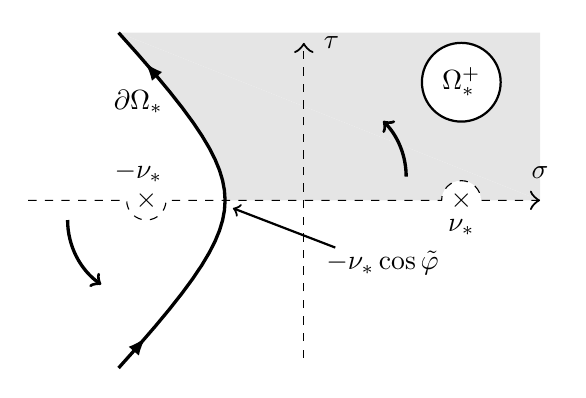
\begin{tikzpicture}
% Remplissage espace Omega_0
\fill [color=gray!20]
(-1,0)
-- plot [domain=0:1.5] ({-cosh(\x)},{sinh(\x)})
-- (3,0)
-- cycle;

\fill [color=gray!20]
({-cosh(1.5)},{sinh(1.5)})
-- plot [domain= 0:-3.0] ({-\x},{sinh(1.5)})
-- (3,0)
-- cycle;

\fill [color=white] (2,0) circle (0.25);

\node at (2,0) {$\times$}; % Pole
\node at (2,-0.35) {$\nu_*$};
\node at (-2,0) {$\times$};
\node at (-2.1,0.35) {$-\nu_*$}; %pole
\node at (3,0.35) {$\sigma$};
\node at (0.35,2) {$\tau$};
\draw[dashed,decoration={ markings, mark=at position 1 with {\arrow[scale=2]{>}}}, postaction={decorate}]
      (-3.5,0) -- (-2.25,0)  arc (-180:0:0.25)  -- (1.75,0)arc (180:0:0.25) -- (3,0); % ca c'est l'axe

\draw[dashed,decoration={ markings, mark=at position 1 with {\arrow[scale=2]{>}}}, postaction={decorate}]
(0,-2)--(0,2);

% Flèches indiquant le sens de déformation de contour
\draw[ very thick, ->] (-3,-0.25) arc (180:235:1);
%\node at (-3.2,-0.9) {$\mathbf{F_1}$};
\draw[ very thick, ->] (1.3,0.3) arc (0:45:1); %ici c'est les fleches 
%\node at (1.5,0.8) {$\mathbf{F_2}$};

% Hyperbole (contour  partial_Omega_0 )
\draw[black, very thick,decoration={ markings,  % This schema allows for fine-tuning the positions of arrows 
      mark=at position 0.1 with {\arrow{latex}},
      mark=at position 0.9 with {\arrow{latex}}},
      postaction={decorate}][domain=-1.5:1.5] plot({-cosh(\x)}, {sinh(\x)});
\node at (-2.1,1.25) {$\partial \Omega_*$};
\node at (1,-0.8) {$-\nu_*\cos \tilde{\varphi}$};

\draw[ thick, ->] (0.4,-0.6)--(-0.9,-0.1);


% Espace Omega_0
\fill [color=white] (2,1.5) circle (0.5);
\draw[thick] (2,1.5) circle (0.5);
\node at (2,1.5) {$\Omega_*^+$};

\end{tikzpicture}
}
\caption{Domain $\Omega_*^+$ and contour $\partial \Omega_*$ in the complex plane $\xi=\sigma+i\tau$. The curved arrows indicate the contour deformation from $\Gamma_0$ to $\partial \Omega_*$}
\label{domega0}
\end{figure}

In order to extract the poles of the spectral functions, it is necessary to determine the action of operators $\mathbf{DM}$ and $\mathbf{TM}$ on a simple pole. In order to do so, contour $\Gamma_0$ in \eqref{B1DM} is deformed into contour $\Gamma_1$ (see Fig.~\ref{gamma1}) and Cauchy's residue theorem is applied, yielding, for
$ V\in\mathbb{C}^2, \, z\in \mathbb{C} \backslash  \rbrack - \infty, -1 \rbrack , \,  z \notin \{\nu_L,\nu_T \}, \, \mbox{Im} z \geq 0, \, \xi \in \Omega_*^+, \, \mbox{Im} \xi <0 $
\begin{equation}
\int_{\Gamma_0} \textbf{DM}(\xi,\zeta).\frac{V}{\zeta-z}\,d\zeta = \frac{\textbf{dm}(z).V}{\xi-z}+D_p(z,\xi),
\label{GaussDM}
\end{equation}
where
\begin{equation}
D_p(z,\xi)= \int_{\Gamma_1} \frac{\textbf{DM}(\xi,\zeta)}{\zeta-z}.V\,d\zeta
\label{defDp}
\end{equation}
Similarly, we deform contour $\Gamma_0$ in \eqref{B2TM} into contour $\partial \Omega_*$, represented Fig. \ref{domega0} and apply once again Cauchy's residue theorem:
\begin{equation}
\int_{\Gamma_0} \textbf{TM}(\xi,\zeta).\frac{1}{\zeta-z}\,d\zeta = \sum_{*=L,T} \frac{\textbf{tm}_*(z).V}{\xi-T_*(z)}\textbf{1}_{\Omega_*}(z)+T_p(z,\xi)
\label{GaussTM}
\end{equation}
where $\textbf{1}_{\Omega_*}(z)=1$ if $z\in\Omega_*^+$ and $0$ elsewhere and
\begin{equation}
T_p(z,\xi)= \frac{1}{2i\pi} \sum_{*=L,T} \int_{\partial \Omega_*} D_*(\xi,\zeta) .\frac{\textbf{tm}_*(\zeta)}{\zeta-z}.V\, d\zeta
\label{defTp}
\end{equation}

\begin{figure}
\centering
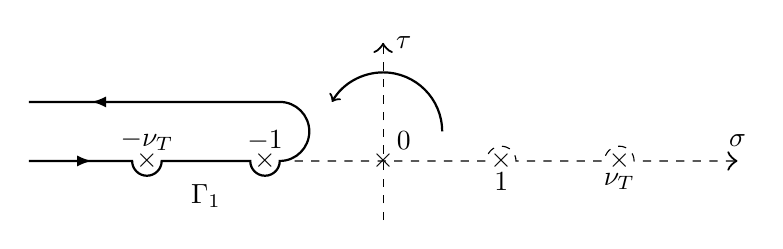
\begin{tikzpicture}[scale=0.75]
\node at (0,0) {$\times$};
\node at (0.35,0.35) {$0$};
\node at (2,0) {$\times$}; % Pole
\node at (4,0) {$\times$}; %pole
\node at (2,-0.35) {$1$};
\node at (4,-0.35) {$\nu_T$};

\node at (-2,0) {$\times$};
\node at (-4,0) {$\times$};
\node at (-2,0.35) {$-1$}; %pole
\node at (-4,0.35) {$-\nu_T$}; %pole
\node at (-3,-0.6) {$\Gamma_1$};

\node at (6,0.35) {$\sigma$};
\node at (0.35,2) {$\tau$};

\draw[dashed, decoration={markings,
 mark=at position 1.0 with {\arrow[scale=2]{>}}},
      postaction={decorate}] (-1.5,0) --(1.75,0) arc(180:0:0.25)--(3.75,0) arc(180:0:0.25)-- (6,0);
      
\draw[dashed, decoration={markings,
 mark=at position 1.0 with {\arrow[scale=2]{>}}},
      postaction={decorate}] (0,-1) -- (0,2);
      
\draw[ thick, ->] (1,0.5) arc (0:150:1);

\draw[thick, black, yshift=0pt,
decoration={ markings,  % This schema allows for fine-tuning the positions of arrows 
      mark=at position 0.1 with {\arrow{latex}},
      mark=at position 0.9 with {\arrow{latex}}},
      postaction={decorate}]
      (-6,0) -- (-4.25,0)  arc (-180:0:0.25) -- (-2.25,0)  arc (-180:0:0.25) -- (-1.75,0) arc(-90:90:0.5)  -- (-6,1);
\end{tikzpicture}
\caption{Contour $\Gamma_1$ in the complex plane $\xi=\sigma+i\tau$. The curved arrow indicates the contour deformation from $\Gamma_0$ to $\Gamma_1$}
\label{gamma1}
\end{figure}

Croisille and Lebeau \cite{CroisilleLebeau} proved that $D_p(z,\cdot)$ and $T_p(z,\cdot)$ belong to a special class of functions $\mathcal{H}^2$ defined hereafter

%\begin{mydef}
%\label{defHpl}
%$H^+$ is the space of functions f which are analytical in $\{z \in \mathbb{C}, \; \mbox{Im} z <0\}$  and verify :
%\begin{equation}
%\underset{c>0}{sup} \int_{-\infty}^{+\infty} |f(x-ic)|^2\,dx<+\infty
%\end{equation}
%\end{mydef}
%\begin{mydef}
%\label{defH}
%$\mathcal{H}$ is the space of the functions f analytical in $\mathbb{C}\backslash \rbrack -\infty,-1\rbrack$ such that $\forall \epsilon \in \rbrack0,\pi \lbrack, f(e^{i\epsilon} \cdot)\in H^+$.
%\end{mydef}

%Afin d'énoncer la nature des décompositions recherchées pour les fonctions spectrales, on définit tout d'abord un ensemble $Z^j(\cdot,\cdot)$. On commence par poser
%\begin{equation}
%Z_0^1=\{\nu_{\alpha}\cos \theta_{inc} \} \hspace{3em} Z_0^2=\{\nu_{\alpha} \cos(\varphi-\theta_{inc}) \}
%\end{equation}
%Les ensembles suivants sont définis par récurrence sur $l \geq 0$ :
%\begin{eqnarray}
%\left\{
%\begin{array}{l}
%Z^1_{l+1} =T_L(Z_l^2 \cap \Omega_L) \cup T_T(Z_l^2 \cap \Omega_T) \\
%Z^2_{l+1} =T_L(Z_l^1 \cap \Omega_L) \cup T_T(Z_l^2 \cap \Omega_T)
%\end{array}
%\right.
%\end{eqnarray}
%et enfin:
%\begin{equation}
%Z^j(\nu_{\alpha}\cos \theta_{inc},\nu_{\alpha}\cos(\varphi-\theta_{inc}))=\bigcup_{l\geq 0} Z^j_l(\nu_{\alpha}\cos \theta_{inc},\nu_{\alpha}\cos(\varphi-\theta_{inc})) \hspace{2em} j=1,2
%\end{equation}
%On admet l'hypothèse $(H)$ suivante :
%\begin{equation*}
%(H) \hspace{3em}  \{ \nu_L, \nu_T, \nu_R \} \cap Z^j(\nu_{\alpha}\cos \theta_{inc},\nu_{\alpha}\cos(\varphi-\theta_{inc})) = \emptyset, \hspace{3em} j=1,2
%\end{equation*}
%
%Il a été démontré par Kamotski et Lebeau \cite{Lebeau2} que, si l'hypothèse $(H)$ est vérifiée, alors les focntions spectrales peuvent se décomposer de la façon suivante :
%\begin{equation}
%\Sigma_j(\xi)=y_j(\xi)+X_j(\xi)
%\end{equation}
%avec $y_j$ singulière et $X_j$ régulière. 
%\paragraph{}
%Plus précisément, la fonctions $y_j$ est méromorphe et ses pôles sont dans $Z^j(Z^1_0,Z^2_0)$  et $X_j \in \mathcal{H}$ tel que ses valeurs limites $X_j(\xi-i0),\; \xi \in\mathbb{R}$ soient analytiques pour $\xi \notin \{-\nu_R,-\nu_T\} \cup Z^j(-\nu_L,-\nu_L)$.
%
%Nous allons maintenant voir comment calculer la partie singulière puis la partie régulière de cette décomposition.
%
%\subsubsection{Expression analytique des pôles et résidus des fonctions spectrales}
%\label{decomp}

Let us now extract all the poles and corresponding residues from the spectral functions, using system \eqref{equationsintegrales}. We begin by defining $X'_j$ by :
\begin{equation}
\Sigma_j(\xi)= \frac{V_j^{(0)}}{\xi-Z^{(0)}_j}+X'_j(\xi), \, \, \, j=1,2,
\label{firstep}
\end{equation}
where $V_j^{(0)}$ is unknown and $Z_1^{(0)}=\nu_{\alpha} \cos \theta_{inc}, \, Z_2^{(0)}=\nu_{\alpha} \cos(\varphi-\theta_{inc})$. Substituting \eqref{firstep} into \eqref{equationsintegrales} and applying formula \eqref{GaussDM} yields :
\begin{equation}
\left\{
\begin{matrix}
\textbf{DM}(X'_1)+\textbf{TM}(X'_2)+\textbf{TM}(\frac{V_2^{(0)}}{\xi-Z_2^{(0)}})=\frac{W^1}{\xi-Z_1^{(1)}}-\frac{\textbf{dm}(Z_1^{(0)}).V_1^{(0)}}{\xi-Z_1^{(0)}}-D_p(Z_1^{(0)},\xi).V_1^{(1)}\\
\textbf{TM}(X'_1)+\textbf{DM}(X'_2)+\textbf{TM}(\frac{V_1^{(0)}}{\xi-Z_1^{(0)}})=\frac{W^2}{\xi-Z_2^{(0)}}-\frac{\textbf{dm}(Z_2^{(0)}).V_2^{(0)}}{\xi-Z_2^{(0)}}-D_p(Z_2^{(0)},\xi).V_2^{(0)}
\end{matrix}
\right.
\end{equation}
In order to only have regular terms on the right-hand side of this system, we chose:
\begin{equation}
V_j^{(0)}=\textbf{dm}^{-1}(Z_j^{(0)}).W^j
\end{equation}
We have $\mbox{det}(\textbf{dm}(z) )\neq 0$ as long as $z\neq \nu_R$. In the following, we will suppose that this is the case. Physically, this means that the incident wave is not a Rayleigh wave and neither are any of the waves reflected by the wedge faces. Furthermore, we suppose that the hypothesis $z \notin \{ \nu_L, \nu_T\}$ that has been made in \eqref{GaussDM} and \eqref{GaussTM} remains true for all the poles. This means that neither the incident, nor any of the reflected waves is an incoming grazing one. Kamotski \cite{KamotskiCrit} proves existence and uniqueness of the solution in the case where this is not true.
%We now have :
%\begin{equation}
%\left\{
%\begin{matrix}
%\textbf{DM}(X'_1)+\textbf{TM}(X'_2)+\textbf{TM}(\frac{V_2^{(0)}}{\xi-Z_2^{(0)}})=-D_p(Z_1^{(0)},\xi).V_1^{(1)}\\
%\textbf{TM}(X'_1)+\textbf{DM}(X'_2)+\textbf{TM}(\frac{V_1^{(0)}}{\xi-Z_1^{(0)}})=-D_p(Z_2^{(0)},\xi).V_2^{(0)}
%\end{matrix}
%\right.
%\label{mille}
%\end{equation}

Applying \eqref{GaussTM}, two new poles appear :
\begin{equation}
Z^{(1)}_{j,L}=T_L(Z_j^{(0)}) \,\;\mbox{ et }\,\; Z^{(1)}_{j,T}=T_T(Z_j^{(0)})
\end{equation}
This leads to the definition of $X''_j$:
\begin{equation}
X'_j=X''_j+\frac{V_{j,L}^{(1)}}{\xi-Z_{j,L}^{(1)}}+\frac{V_{j,T}^{(1)}}{\xi-Z_{j,T}^{(1)}},
\end{equation}
where $V_{j,L}^{(1)}$ and $V_{j,T}^{(1)}$ are unknown vectors. Once again, we substitute this into the system and apply (\ref{GaussDM}). 
% Once again, we substitute this into (\ref{mille}) and apply (\ref{GaussDM}). 
Residues $V_{j,*}^{(1)}$ are chosen so as to only have regular terms on the left-hand side of the system:
\begin{equation}
V_{j,*}^{(1)}=-\textbf{dm}^{-1}(T_*(Z_{3-j}^{(0)})).\textbf{tm}_*(Z_{3-j}^{(0)}).V_{3-j}^{(0)}\mathbf{1}_{\Omega_*}(Z_{3-j}^{(0)})
\end{equation}
These steps are repeated recursively as long as the poles $Z_{j,L}^{(k)} \in \Omega_L^+$ and $Z_{j,T}^{(k)} \in \Omega_T^+$. When this is the case, \eqref{GaussTM} can be applied, creating new poles in the right-hand side of the system. These new poles are then extracted from the spectral functions using \eqref{GaussDM}, and so on. In the end, we have, for $\mbox{Im}\, \xi <0$ :
\begin{gather}
\Sigma_j(\xi)=Y_j(\xi)+X_j(\xi) \label{decomp}\\
Y_j(\xi)=\sum_k \sum_{*=L,T} \frac{V_{j,*}^{(k)}}{\xi-Z_{j,*}^{(k)}}
\label{yj},
\end{gather}
where
\begin{equation}
\begin{matrix}
Z_{1}^{(0)}=\nu_{\alpha} \cos \theta_{inc},  & Z_{2}^{(0)}=\nu_{\alpha} \cos(\varphi-\theta_{inc}) \\
Z_{j,L}^{(k+1)}= T_L(Z_{3-j,*}^{(k)}) &Z_{j,T}^{(k+1)}= T_T(Z_{3-j,*}^{(k)}) 
\end{matrix}
\end{equation}
and
\begin{equation}
\begin{matrix}
V_{j}^{(0)}=\textbf{dm}^{-1}(Z_{j}^{(0)}).W_j^{\alpha}\\
V_{j,L}^{(k+1)}=-\textbf{dm}^{-1}(Z_{j,*}^{(k+1)}).\textbf{tm}_L(Z_{3-j,*}^{(k)}).V_{3-j,*}^{(k)}.\textbf{1}_{\Omega_L}(Z_{3-j,*}^{(k)}) \\ 
V_{j,T}^{(k+1)}=-\textbf{dm}^{-1}(Z_{j,*}^{(k+1)}).\textbf{tm}_T(Z_{3-j,*}^{(k)}).V_{3-j,*}^{(k)}.\textbf{1}_{\Omega_T}(Z_{3-j,*}^{(k)}) 
\end{matrix}
\label{residus}
\end{equation}
The recursive procedure stops when the poles $Z_{j,*}^{(k)}$ exit $\Omega_L^+\cup\Omega_T^+$ (\textit{i.e.} when the translation operators $T_L$ and $T_T$ can no longer be applied to them). Croisille and Lebeau \cite{CroisilleLebeau} have shown that this defines a finite number of poles. Physically, this means that an incident ray exits the wedge after a finite number of reflections and mode conversions. We have thus extracted all the poles from the spectral functions and have computed them analytically, along with their corresponding residues. 

\subsection{Regular part}
\label{regpart}
The singular parts $Y_j$ of the spectral functions having been determined, two new functions $X_1$ and $X_2$ are defined by \eqref{decomp}. In the following, a numerical approximation method for $X_j$ is proposed. In order to do so, a system of functional equations solved by $X_1, X_2$ is derived by subtracting vector
\begin{equation}
\begin{pmatrix}
\textbf{DM}(Y_1)+\textbf{TM}(Y_2) \\
\textbf{TM}(Y_1)+\textbf{DM}(Y_2)
\end{pmatrix},
\end{equation}
where $Y_1$ and $Y_2$ are given by equations \eqref{yj} to \eqref{residus}, from both sides of (\ref{equationsintegrales}) :
\begin{equation}
\left\{ 
\begin{matrix}
\textbf{DM}(X_1)(\xi)+\textbf{TM}(X_2)(\xi)=u_1(\xi)\\
\textbf{TM}(X_1)(\xi)+\textbf{DM}(X_2)(\xi)=u_2(\xi)
\end{matrix}
\right.,
\label{regparteqn}
\end{equation}
with, for $j=1,2$
\begin{equation}
u_j(\xi)=-\sum_k \sum_{*=L,T} \left[ D_p(Z_{j,*}^{(k)},\xi).V_{j,*}^{(k)}+T_p(Z_{3-j,*}^{(k)},\xi).V_{3-j,*}^{(k)}\right]
\label{scndmembre}
\end{equation}
Croisille and Lebeau \cite{CroisilleLebeau} have shown that this system has a unique solution $(X_1,X_2)$ in $\mathcal{H}^2$ (defined in Def.\ref{defH}). In the sequel, a numerical approximation of the regular parts $X_j$ will be computed using a Galerkin collocation method.

The functional space $\mathcal{H}$ is approached by a finite-dimension space generated by the basis functions $\varphi_k$:
\begin{equation}
\varphi_k(\xi)= \sqrt{\frac{a_k}{\pi}} \frac{1}{\xi+a_k} \; \; (a_k)_{1 \leq k \leq N} \in (\lbrack 1, + \infty \lbrack)^N
\end{equation}
In this space, functions $X_j$ are approximated by
\begin{equation}
X_j(\xi) \approx \sum_{k=1}^N \tilde{X}_j^k \varphi_k(\xi), \; \tilde{X}_j^k \in \mathbb{C}^2 \;, j=1,2
\label{Xj}
\end{equation}
Substituting this approximation into \eqref{regparteqn} and applying 
%\begin{equation}
%\left\{
%\begin{matrix}
%\sum_{k=1}^N \tilde{X}_1^k \int_{\Gamma_0} \textbf{DM}(\xi,\zeta) \varphi_k(\zeta) \, d \zeta +\tilde{X}_2^k \int_{\Gamma_0} \textbf{TM}(\xi,\zeta) \varphi_k(\zeta) \, d \zeta \approx u_1(\xi) \\
%~\\
%\sum_{k=1}^N \tilde{X}_1^k \int_{\Gamma_0} \textbf{TM}(\xi,\zeta) \varphi_k(\zeta) \, d \zeta +\tilde{X}_2^k \int_{\Gamma_0} \textbf{DM}(\xi,\zeta) \varphi_k(\zeta) \, d \zeta \approx u_2(\xi)
%\end{matrix}
%\right.
%\end{equation}
variable change $\zeta=iy$ to this system before evaluating it at points $\xi=b_1,...,b_N$ leads to the following linear system of equations :
\begin{equation}
\left\{
\begin{matrix}
\sum_{k=1}^N \tilde{X}_1^k \int_{-\infty}^{+\infty} \textbf{DM}(b_1,iy)e_{a_k}(y) \, dy + \tilde{X}_2^k \int_{-\infty}^{+\infty} \textbf{TM}(b_1,iy)e_{a_k}(y) \, dy=u_1(b_1) \\
\vdots\\
\sum_{k=1}^N \tilde{X}_1^k \int_{-\infty}^{+\infty} \textbf{TM}(b_N,iy)e_{a_k}(y) \, dy + \tilde{X}_2^k \int_{-\infty}^{+\infty} \textbf{DM}(b_N,iy)e_{a_k}(y) \, dy=u_2(b_N)
\end{matrix}
\right.,
\label{linsys}
\end{equation}
where
\begin{equation}
e_{a_k}(y)=\sqrt{\frac{a_k}{\pi}} \frac{1}{y-ia_k} , \, 1 \leq k \leq N
\end{equation}
This system can be expressed in terms of matrices
\begin{equation}
\begin{pmatrix}
\mathbb{D}&\mathbb{T}\\
\mathbb{T}&\mathbb{D}
\end{pmatrix}
\begin{pmatrix}
\mathbb{X}_1 \\
\mathbb{X}_2
\end{pmatrix}
=
\begin{pmatrix}
\mathbb{U}_1 \\
\mathbb{U}_2
\end{pmatrix}
\iff
\left\{
\begin{matrix}
(\mathbb{D}+\mathbb{T})(\mathbb{X}_1+\mathbb{X}_2)=\mathbb{U}_1+\mathbb{U}_2\\
(\mathbb{D}-\mathbb{T})(\mathbb{X}_1-\mathbb{X}_2)=\mathbb{U}_1-\mathbb{U}_2
\end{matrix}
\right.
\label{systmat}
\end{equation}
where, for $1\leq l,k \leq N$ :
%\begin{equation}
%\begin{split}
%\mathbb{D}_{lk}&=\int_{-\infty}^{+\infty} \textbf{DM}(b_l,iy)e_{a_k}(y) \, dy \\
%\mathbb{T}_{lk}&=\int_{-\infty}^{+\infty} \textbf{TM}(b_l,iy)e_{a_k}(y) \, dy
%\end{split}
%\label{intDT}
%\end{equation}
%and
%\begin{equation}
%\mathbb{X}_j=
%\begin{pmatrix}
%\tilde{X}_j^1\\
%\vdots \\
%\tilde{X}_j^N
%\end{pmatrix}
%\hspace{3em}
%\mathbb{U}_j=
%\begin{pmatrix}
%u_j(b_1)\\
%\vdots \\
%u_j(b_N)
%\end{pmatrix}
%\end{equation}
%The coefficients of the linear combination \eqref{Xj} are computed by solving system \eqref{linsys} numerically. To do so, the coefficients of the system are computed analytically.

%\subsubsection{Calcul des coefficients de la matrice $\mathbb{D}$}
%Let us now compute coefficients of the linear system. The first coefficients are
%Passons maintenant au calcul effectif des coefficients des matrices de ce système. On a pour commencer, en utilisant (\ref{defDM}) :
\begin{equation}
\begin{split}
\mathbb{D}_{lk}=\int_{-\infty}^{+\infty} \textbf{DM}(b_l,iy)e_{a_k}(y) \, dy &=\frac{1}{2i\pi} \int_{-\infty}^{+\infty} \frac{\mathbf{dm}}{b_l-iy} 
%\begin{pmatrix}
%-1&A(iy) \\
%B(iy)&-1
%\end{pmatrix}
\sqrt{\frac{a_k}{\pi}}\frac{1}{y-ia_k} \, dy \\
&=- \frac{\sqrt{a_k}}{2\pi \sqrt{\pi}}
\begin{pmatrix}
\mathcal{D}_1(a_k,b_l) & \mathcal{D}_2(a_k,b_l) \\
\mathcal{D}_3(a_k,b_l) &\mathcal{D}_1(a_k,b_l)
\end{pmatrix}=\frac{\sqrt{a_k}}{2\pi \sqrt{\pi}}\mathbb{D}(a_k,b_l)
\end{split}
\label{Dab}
\end{equation}
%Using \eqref{defDM}, we can define :
%\begin{equation}
%\mathcal{D}_1(a,b)=\int_{-\infty}^{+\infty} \frac{dy}{(y+ib)(y-ia)} 
%\end{equation}
%\begin{equation}
%\mathcal{D}_2(a,b)=\int_{-\infty}^{+\infty} \frac{-iy(1-2\mu \zeta_L(iy) \zeta_T(iy)+2\mu y^2)}{(y+ib)(y-ia)\zeta_T(iy)} \,dy 
%\end{equation}
%\begin{equation}
%\mathcal{D}_3(a,b)=\int_{-\infty}^{+\infty} \frac{iy(1-2\mu \zeta_L(iy) \zeta_T(iy)+2\mu y^2)}{(y+ib)(y-ia)\zeta_L(iy)} \,dy
%\end{equation}
The explicit expressions of operators $\mathcal{D}_i, 1\leq i\leq3$ and their values are computed in \ref{compD}.
The other coefficients of the system are, for $1\leq l,k \leq N$
\begin{equation}
\begin{split}
\mathbb{T}_{lk}=\int_{-\infty}^{+\infty} \textbf{TM}(b_l,iy)e_{a_k}(y) \, dy 
&=\frac{1}{2i\pi} \int_{-\infty}^{+\infty} \sum_{*=L,T} \frac{\textbf{tm}_* (iy, \mbox{sgn} \sin \varphi)}{b_l-T_*(iy)} \sqrt{\frac{a_k}{\pi}}\frac{1}{y-ia_k}\,dy \\
&=\frac{1}{2i\pi}\sqrt{\frac{a_k}{\pi}}\sum_{*=L,T} \int_{-\infty}^{+\infty} \frac{\textbf{tm}_*(iy,\epsilon)}{\lbrack b_l-(iy \cos \varphi +  \zeta_*(iy)| \sin \varphi|)\rbrack(y-ia_k)} \, dy,
\end{split}
\end{equation}
where $\epsilon= \mbox{sgn}( \sin \varphi)$. Let us define
\begin{equation}
\mathbb{T}_{lk}=\frac{\mu}{2i\pi}\sqrt{\frac{a_k}{\pi}}
\begin{pmatrix}
\mathcal{T}_1^L(a_k,b_l)+ \mathcal{T}_1^T(a_k,b_l)  &  \mathcal{T}_2^L(a_k,b_l) + \mathcal{T}_2^T(a_k,b_l)  \\
 \mathcal{T}_3^L(a_k,b_l)+ \mathcal{T}_3^T(a_k,b_l) &\mathcal{T}_4^L(a_k,b_l)+ \mathcal{T}_4^T(a_k,b_l)
\end{pmatrix}
=\frac{1}{2i\pi}\sqrt{\frac{a_k}{\pi}}\mathbb{T}(a_k,b_l)
\label{Tab}
\end{equation}
The explicit expressions of operators $\mathcal{T}_i^*, 1\leq i\leq4, *=L,T$ and their values are computed in \ref{compT}.

Finally, for $j=1,2$ :
\begin{equation}
\mathbb{X}_j=\begin{pmatrix}
\tilde{X}^1_j \\
\vdots \\
\tilde{X}^1_j
\end{pmatrix}, \,
\tilde{X}^k_j \in \mathbb{C}^2; \hspace{2em}
\mathbb{U}_j=\begin{pmatrix}
u_j(b_1)\\
\vdots \\
u_j(b_N)
\end{pmatrix}, \,
u_j(b_k) \in \mathbb{C}^2
\end{equation}
where $u_j(\xi)$ is given by \eqref{scndmembre}. Applying variable change $\zeta=iy$ to the definition of $D_p$ given by 
\eqref{GaussDM} and substituting \eqref{Dab} in the result gives
\begin{equation}
D_p(z,\xi)=\frac{1}{2\pi}\mathbb{D}(-z,\xi)-\frac{\textbf{dm}(z)}{\xi-z}
\label{Dpscm}
\end{equation}
Similarly, applying variable change $\zeta=iy$ to \eqref{GaussTM} and substituting \eqref{Tab} in the result yields
\begin{equation}
T_p(z,\xi)=\frac{1}{2i\pi}\mathbb{T}(-z,\xi)- \sum_{*=L,T}\frac{\textbf{tm}_*(z,\epsilon)}{b-T_*(z)}\textbf{1}_{\Omega_*}(z)
\label{Tpscm}
\end{equation}
Equations \eqref{Dpscm} and \eqref{Tpscm} are substituted into \eqref{scndmembre}. By construction, the singular terms cancel each other and the remaining terms are :
\begin{equation}
u_j(\xi)=-\frac{1}{2i\pi}\sum_{k}\sum_{*=L,T}\left(i\mathbb{D}(-Z_{j,*}^{(k)},\xi).V_{j,*}^{(k)}+\mathbb{T}(-Z_{3-j,*}^{(k)},\xi).V_{3-j,*}^{(k)} \right) +\frac{W_j^{\alpha}}{\xi-Z_j^{(0)}}
\label{uDT}
\end{equation}

Using these results, the linear system \eqref{systmat} can be implemented and solved numerically thanks to the C++ library Eigen, and an evaluation of the regular part of the spectral functions is obtained. However, for values of $\xi$ lying in certain parts of the complex plane, this evaluation is not sufficiently accurate. The technique used to solve this problem is called the propagation of the solution.

\subsection{Propagation of the solution}
\label{C3:propag}
The method described hereafter is used to ``propagate''  the accuracy of the solution to \eqref{regparteqn} to the whole complex plane. This is done by determining a new system of recursive equations solved by $X_1, X_2$ in which the regular part $X_j$ is expressed using the value of $X_1, X_2$ in a domain where the numerical approximation is valid.

By deforming $\Gamma_0$ into $\Gamma_2$, represented in Fig. \ref{contour2}, the half-plane Im $\xi<0$  is entirely crossed. Note that the branch points $\pm \nu_*, *=L,T$ are not crossed during this deformation, indicated by the curved arrow in Fig.~\ref{contour2}. The contribution of poles $\zeta=\xi, \, \rm Im \xi<0$, is given by Cauchy's integral formula :
\begin{equation}
\int_{\Gamma_0} \textbf{DM}(\xi,\zeta)X_j(\zeta)\, d\zeta = \int_{\Gamma_2}  \textbf{DM}(\xi,\zeta)X_j(\zeta)\, d\zeta + \textbf{dm}(\xi).X_j(\xi)
\label{DM2}
\end{equation}
\begin{figure}[h]
	\centering
	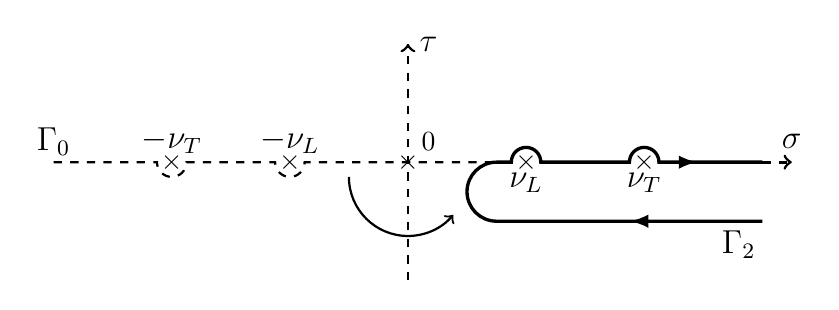
\begin{tikzpicture}[scale=0.75]
	\node at (0,0) {$\times$};
	\node at (0.35,0.35) {$0$};
	\node at (2,0) {$\times$}; 
	\node at (2,-0.35) {\large $\nu_L$};
	\node at (4,0) {$\times$};
	\node at (4,-0.35) {\large $\nu_T$};
	\node at (-2,0) {$\times$};
	\node at (-2,0.35) {\large $-\nu_L$};
	\node at (-4,0) {$\times$};
	\node at (-4,0.35) {\large $-\nu_T$};
	\node at (5.6,-1.4) {\large $\Gamma_2$};
	\node at (0.35,2) {\large $\tau$};
	\node at (6.5,0.35) {\large $\sigma$};
	\node at (-6,0.35) {\large $\Gamma_0$};
	
	\draw[very thick, black,yshift=0pt,
	decoration={ markings,  % This schema allows for fine-tuning the positions of arrows 
		mark=at position 0.2 with {\arrow{latex}},
		mark=at position 0.9 with {\arrow{latex}}},
	postaction={decorate}]
	(6,-1) -- (1.5,-1)  arc (90:-90:-0.5)  -- (1.5,0) -- (1.75,0) arc (180:0:0.25) -- (3.75,0) arc (180:0:0.25) -- (6,0);
	
	\draw[dashed, line width = 0.8pt,yshift=0pt]
	(-6,0) -- (-4.25,0) arc (-180:0:0.25) -- (-2.25,0)  arc (-180:0:0.25)  -- (1.5,0);
	
	\draw[dashed, line width = 1pt,yshift=0pt,
	decoration={ markings,  mark=at position 1 with {\arrow{>}}},
	postaction={decorate}] (0,-2)--(0,2);
	
	\draw[dashed, line width = 1pt,yshift=0pt,
	decoration={ markings,  mark=at position 1 with {\arrow{>}}},
	postaction={decorate}] (6,0)--(6.5,0);
	
	\draw[ thick, ->] (-1,-0.25) arc (180:320:1);
	
	\end{tikzpicture}
	\caption{Integration contour $\Gamma_2$ in the complex place $\xi=\sigma+i\tau$. The curved arrow indicates the contour deformation from $\Gamma_0$ to $\Gamma_2$.}
	\label{contour2}
\end{figure}

It is now necessary to define the inverse transformation operator $T_*^{-1}, *=L,T$ :
\begin{equation}
T_*^{-1}(\xi=\nu_*\cos\theta)=\xi \cos \phiti-\zeta_*(\xi)\sin\phiti=\nu_*\cos(\theta-\tilde{\varphi}).
\end{equation}
In order for the cosine in this translation operator to be well defined, it is necessary to impose
\begin{equation}
\xi \in \Omega_*^-=\{\xi=\nu_*\cos\theta, \, \, \, \tilde{\varphi}\leq \mbox{Re}\theta\leq\pi, \, \, \, \mbox{Im}\xi< 0\},
\end{equation}
where $\Omega_*^-$ is represented in Fig.~\ref{dOmegamoins}. By deforming contour $\Gamma_0$ into contour $\partial \Omega_*^-$ (also represented in Fig.~\ref{dOmegamoins}), domain $\Omega_*^-$ is crossed. The contribution of poles $\zeta=T_*^{-1}(\xi)$, when $\xi\in\Omega_*^-$  is taken into account using Cauchy's integral formula :
\begin{equation}
\int_{\Gamma_0} \textbf{TM}(\xi,\zeta)X_j(\zeta)\, d\zeta = \int_{\partial \Omega_*^-}  \textbf{TM}(\xi,\zeta)X_j(\zeta)\, d\zeta+\sum_{*=L,T} \mathbf{M}_*(\xi).X_j(T^{-1}_*(\xi))\textbf{1}_{\Omega_*^-}(\xi),
\label{TM2}
\end{equation}
where $\textbf{1}_{\Omega_*^-}(\xi)=1$ when $\xi \in \Omega_*^-$ and $0$ elsewhere and
\begin{equation}
\mathbf{M}_*(\xi=\nu_*\cos\theta)=-\frac{\sin(\theta-\tilde{\varphi})}{\sin\theta} \textbf{tm}_*(T_*^{-1}(\xi))
\end{equation}

\begin{figure}[ht]%
\begin{center}
	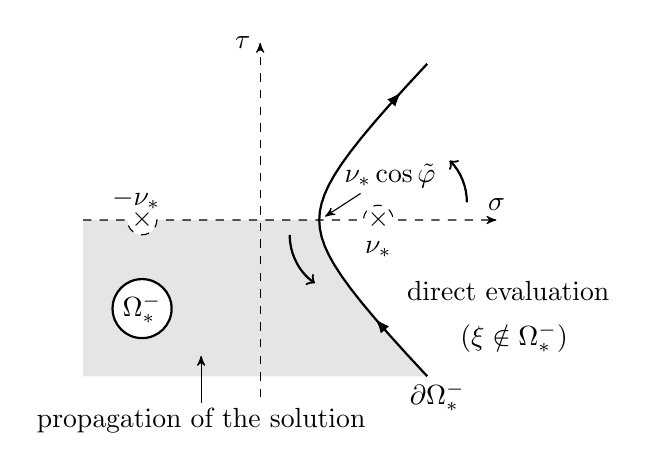
\begin{tikzpicture}[scale=0.75]
	% Filling Omega_*^-
	\fill [color=gray!20]
	(-1,0)
	-- plot [domain= 0:1.7] ({cosh(\x)},{-sinh(\x)})
	-- (-3,0)
	-- cycle;
	
	\fill [color=gray!20]
	({cosh(1.7)},{-sinh(1.7)})
	-- plot [domain= 0:-3] ({\x},{-sinh(1.7)})
	-- (-3,0)
	-- cycle;
	
	\fill[color=white] (-2,0) circle (0.25);
	
	\draw[dashed, ->,>=stealth'] (-3,0)  -- (-2.25,0) arc(-180:0:0.25)--(1.75,0) arc (180:0:0.25)--(4,0) node[above]{$\sigma$};
	\draw[dashed, ->,>=stealth'](0,-3)--(0,3) node[left]{$\tau$};
	\node at (2,0) { $\times$}; 
	\node at (2,-0.5) {$\nu_*$};
	\node at (-2,0) { $\times$};
	\node at (-2.1,0.35) {$-\nu_*$};
	
	% Hyperbola (contour  partial_Omega_0 )
	\draw[black, thick,decoration={ markings,  % This schema allows for fine-tuning the positions of arrows 
		mark=at position 0.2 with {\arrow{latex}},
		mark=at position 0.9 with {\arrow{latex}}},
	postaction={decorate}][domain=-1.7:1.7] plot({cosh(\x)}, {sinh(\x)});
	
	\node at (3,-3) {$\partial \Omega_*^-$};
	\draw[thin, ->,>=stealth'](1.7,0.45) -- (1.1, 0.06);
	\node at (2.2, 0.75) { $\nu_*\cos \tilde{\varphi}$};
	
	% Omega_0
	\draw[->,>=stealth'] (-1,-3.1) -- (-1,-2.3);
	\node at (-1,-3.4) {propagation of the solution};
	\node at (4.2,-1.2) {direct evaluation};
    \node at (4.3,-2) { $(\xi \notin \Omega_*^-)$};

	% Espace Omega_0
\fill [color=white] (-2,-1.5) circle (0.5);
\draw[thick] (-2,-1.5) circle (0.5);
\node at (-2,-1.5) {$\Omega_*^-$};

\draw[thick, ->] (0.5,-0.25) arc (180:235:1);
\draw[thick, ->] (3.5,0.3) arc (0:45:1); %ici c'est les fleches 
	
	\end{tikzpicture}
\end{center}
\caption{Domain $\Omega_*^-$ and contour $\partial \Omega_*^-$ in the complex plane $\xi=\sigma + i \tau$. The curved arrows indicate contour deformation from $\Gamma_0$ to $\partial \Omega_*^-$. }
\label{dOmegamoins}
\end{figure}
The recursive system of functional equations solved by the regular part is obtained by substituting \eqref{DM2} and \eqref{TM2} into \eqref{regparteqn}:
\begin{equation}
\left\{
\begin{matrix}
X_1(\xi) =g_1(\xi)-\textbf{dm}^{-1}(\xi).\underset{*=L,T}{\sum} \mathbf{M}_*(\xi).X_2(T_*^{-1}(\xi))\textbf{1}_{\Omega_*^-}(\xi) \\
X_2(\xi) =g_2(\xi)-\textbf{dm}^{-1}(\xi).\underset{*=L,T}{\sum} \mathbf{M}_*(\xi).X_1(T_*^{-1}(\xi))\textbf{1}_{\Omega_*^-}(\xi)
\end{matrix}
\right.,
\label{recur}
\end{equation}
where , for $j=1,2$
\begin{equation}
g_j(\xi)=\textbf{dm}^{-1}(\xi)\left( u_j(\xi)- \int_{\Gamma_2}  \textbf{DM}(\xi,\zeta)X_j(\zeta)\, d\zeta- \int_{\partial \Omega_*^-}  \textbf{TM}(\xi,\zeta)X_{3-j}(\zeta)\, d\zeta \right) 
\label{g1g2}
\end{equation}

This new recursive system is used to evaluate the spectral functions in the domain $W=\{ \mbox{Im}(\xi)<0, \xi \notin \partial \Omega_*^- \}$. To do so, functions $g_j$ must be evaluated numerically.

Each of the integrals appearing in the definition of $g_j$ are evaluated separately using the approximation of the regular part \eqref{Xj} for the computation of terms $X_j(\zeta)$ and $X_{3-j}(\zeta)$. 

Substituting \eqref{Dab} into \eqref{DM2} yields :
\begin{equation}
\int_{\Gamma_2}\textbf{DM}(\xi,\zeta)\varphi_k(\zeta) \, d\zeta = \int_{\Gamma_0}\textbf{DM}(\xi,\zeta)\varphi_k(\zeta)\, d\zeta -\textbf{dm}(\xi).\varphi_k(\xi)=\frac{1}{2\pi}\sqrt{\frac{a_k}{\pi}} \mathbb{D}(a_k,\xi)-\textbf{dm}(\xi).\varphi_k(\xi) 
\label{NDreg}
\end{equation}
and substituting \eqref{Tab} into \eqref{TM2} yields:
\begin{equation}
\begin{split}
\int_{\partial \Omega_*^-}  \textbf{TM}(\xi,\zeta)\varphi_k(\zeta)\, d\zeta&=\int_{\Gamma_0} \textbf{TM}(\xi,\zeta)\varphi_k(\zeta)\, d\zeta  -\sum_{*=L,T} \mathbf{M}_*(\xi).\varphi_k(T^{-1}_*(\xi)) \\
= &\frac{1}{2i\pi} \sqrt{\frac{a_k}{\pi}} \mathbb{T}(a_k,\xi)- \sum_{*=L,T}\mathbf{M}_*(\xi).\varphi_k(T^{-1}_*(\xi))\textbf{1}_{\Omega_*^-}(\xi)
\end{split}
\label{NTreg}
\end{equation}
Finally, \eqref{NDreg} and \eqref{NTreg} can be injected into \eqref{g1g2} :
\begin{equation}
\textbf{dm}(\xi).g_j(\xi)=u_j(\xi)-\sum_{k=1}^N \sqrt{\frac{a_k}{\pi}}\left( \mathbb{ND}(a_k,\xi).\tilde{X}_j^k+\mathbb{NT}(a_k,\xi).\tilde{X}_{3-j}^k \right) ,
\label{gjfinal}
\end{equation}
where
\begin{equation}
\mathbb{ND}(a,b)=\frac{1}{2\pi}\mathbb{D}(a,b)-\frac{\textbf{dm}(b)}{a+b}
\label{defND}
\end{equation}
and
\begin{equation}
\mathbb{NT}(a,b)=\frac{1}{2i\pi}\mathbb{T}(a,b)-\sum_{*=L,T}\frac{\mathbf{M}_*(b)}{T^{-1}_*(b)+a} .
\end{equation}

In system \eqref{recur}, the value of the regular part of the spectral function in domain $\Omega_*^-$, visible Fig.~\ref{dOmegamoins}, is expressed using its value in the domain $\xi \notin \Omega_*^-$, where the numerical approximation \eqref{Xj} is valid. To do so, functions $g_j,\, j=1,2$ are evaluated using \eqref{gjfinal}. The accuracy of the numerical evaluation in domain $\xi \notin \Omega_*^-$ is therefore propagated to domain $\Omega_*^-$. 

This concludes the semi-analytical computation of the spectral functions. Numerical comparisons with other codes are presented in the following.


\section{Numerical validation}
The longitudinal and transversal diffraction coefficients are computed using \eqref{DL} and \eqref{DT}. The spectral functions are evaluated in $\xi=\nu_*\cos\theta -i10^{-8}$ (a small negative imaginary part is added to ensure that the recursive equations \eqref{recur} are valid). This is achieved by, first, computing the poles and residues of the spectral functions analytically using the recursive algorithm described in subsection \ref{singpart}. Then, the regular parts of the spectral functions are approached numerically by solving \eqref{regparteqn} thanks to the Galerkin collocation method described in subsection \ref{regpart}, where the Galerkin parameters are set to:
\begin{equation}
a_k=1.0001+0.05e^{k\frac{\log 10}{4}}-1, \hspace{3em} b_k=a_k-0.1i, \hspace{3em} 1\leq k\leq20
\end{equation}
Finally, the solution is rendered accurate in the entire complex domain by applying the recursive procedure called the propagation of the solution described in subsection \ref{C3:propag}.

Following these steps, the diffraction coefficients have been computed every $0.2 ^o$ for a steel wedge in which $c_L=5700 m.s^{-1}, c_T=3100 m.s^{-1}$. The results are presented hereafter.
\subsection{For $\varphi<\pi$}
For wedge angles $\varphi<\pi$, the \acrfull{lt} code of Gautesen and Fradkin \cite{GautesenFradkin}, based on the method briefly recalled in \ref{C1:lt} has been used to validate the results of the \acrfull{sf} method. 

Fig.~\ref{8055} shows the absolute value of the diffraction coefficients  with respect to the observation angle obtained for a wedge of angle $\varphi=80^o$ illuminated by a wave incident with an angle $\theta_{inc}=55^o$. The green line represents the diffraction coefficients obtained using only the singular parts $Y_j$ of the spectral functions. The dark blue line is the diffraction coefficient obtained using the \acrshort{lt} code and the red circles represent the result obtained using the \acrshort{sf} code. These two plots are perfectly overlapping. The singular part alone, however, is not sufficient to compute accurate coefficients. 

Fig.~\ref{16040} shows the absolute value of the diffraction coefficients with respect to the observation angle obtained for a wedge of angle $\varphi=160^o$ illuminated by a wave incident with an angle $\theta_{inc}=40^o$. The light blue line represents the diffraction coefficients obtained without applying the ``propagation of the solution'' technique for the \acrshort{sf} code. The dark blue line is the diffraction coefficient obtained using the \acrshort{lt} code and the red circles represent the result obtained using the \acrshort{sf} code, including the ``propagation of the solution'' technique. These two plots are perfectly overlapping. Furthermore, the ``propagation of the solution'' technique is necessary in order to avoid coefficients which diverge near the wedge faces. 

\begin{figure}%[h!]
\centering
    \begin{subfigure}[b]{0.44\textwidth}
        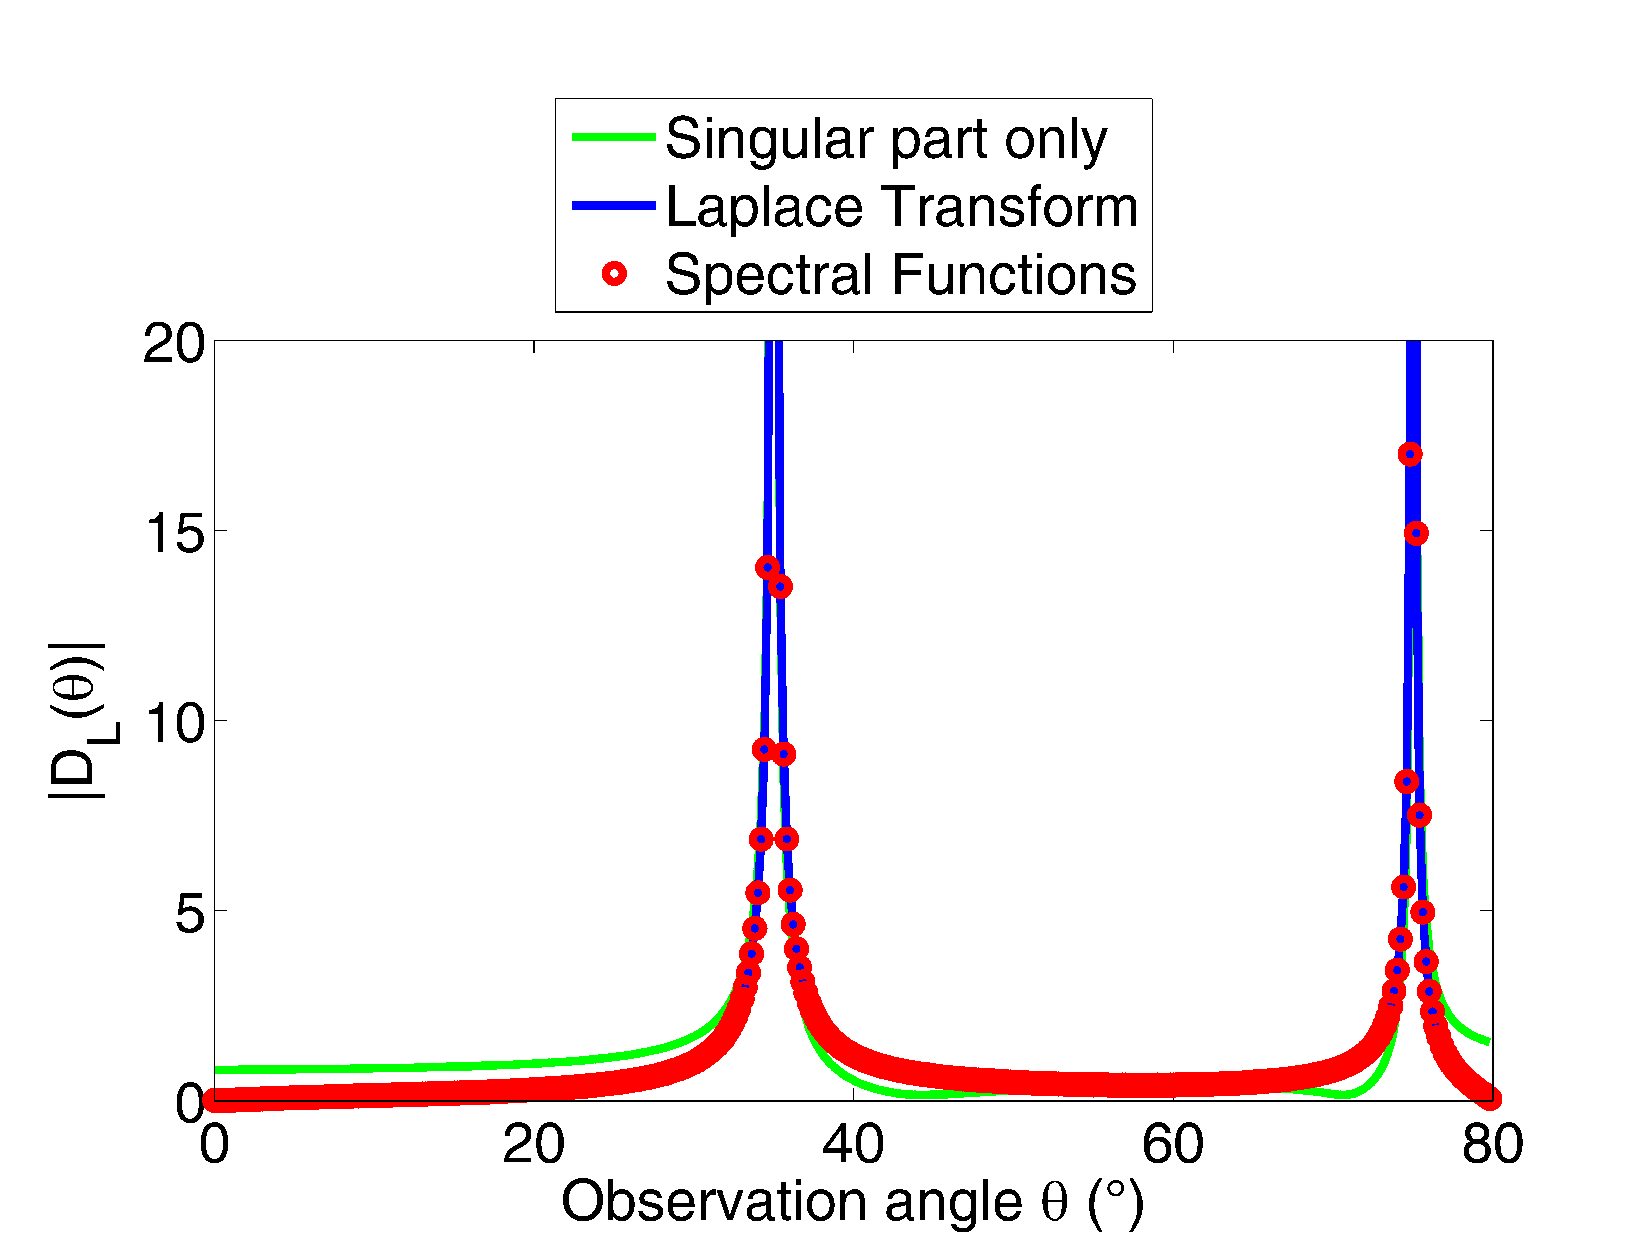
\includegraphics[width=\textwidth]{images/chapter3/Figure8a.pdf}
        \caption{Diffracted and incident L waves}
    \end{subfigure}  
    \begin{subfigure}[b]{0.44\textwidth}
        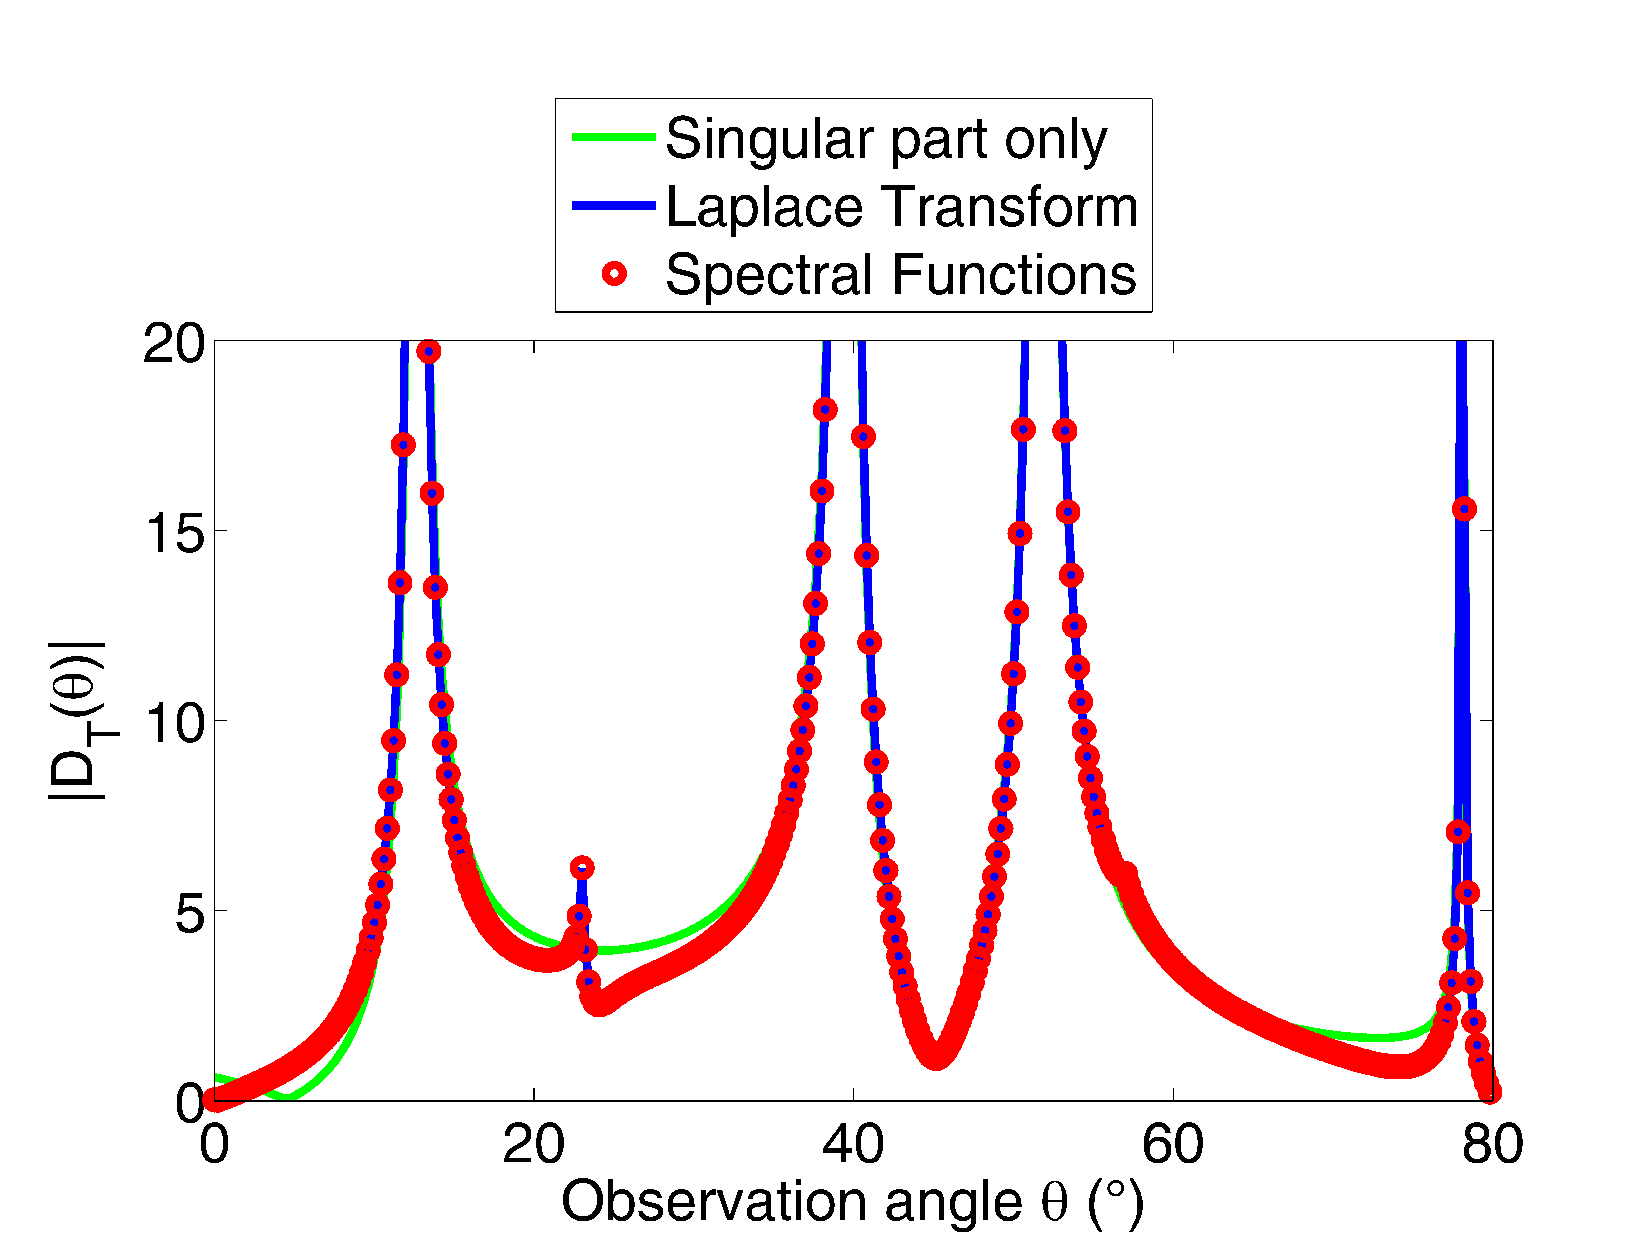
\includegraphics[width=\textwidth]{images/chapter3/Figure8b.pdf}
        \caption{Diffracted T wave and incident L wave}
     \end{subfigure} \\   
     \begin{subfigure}[b]{0.44\textwidth}
        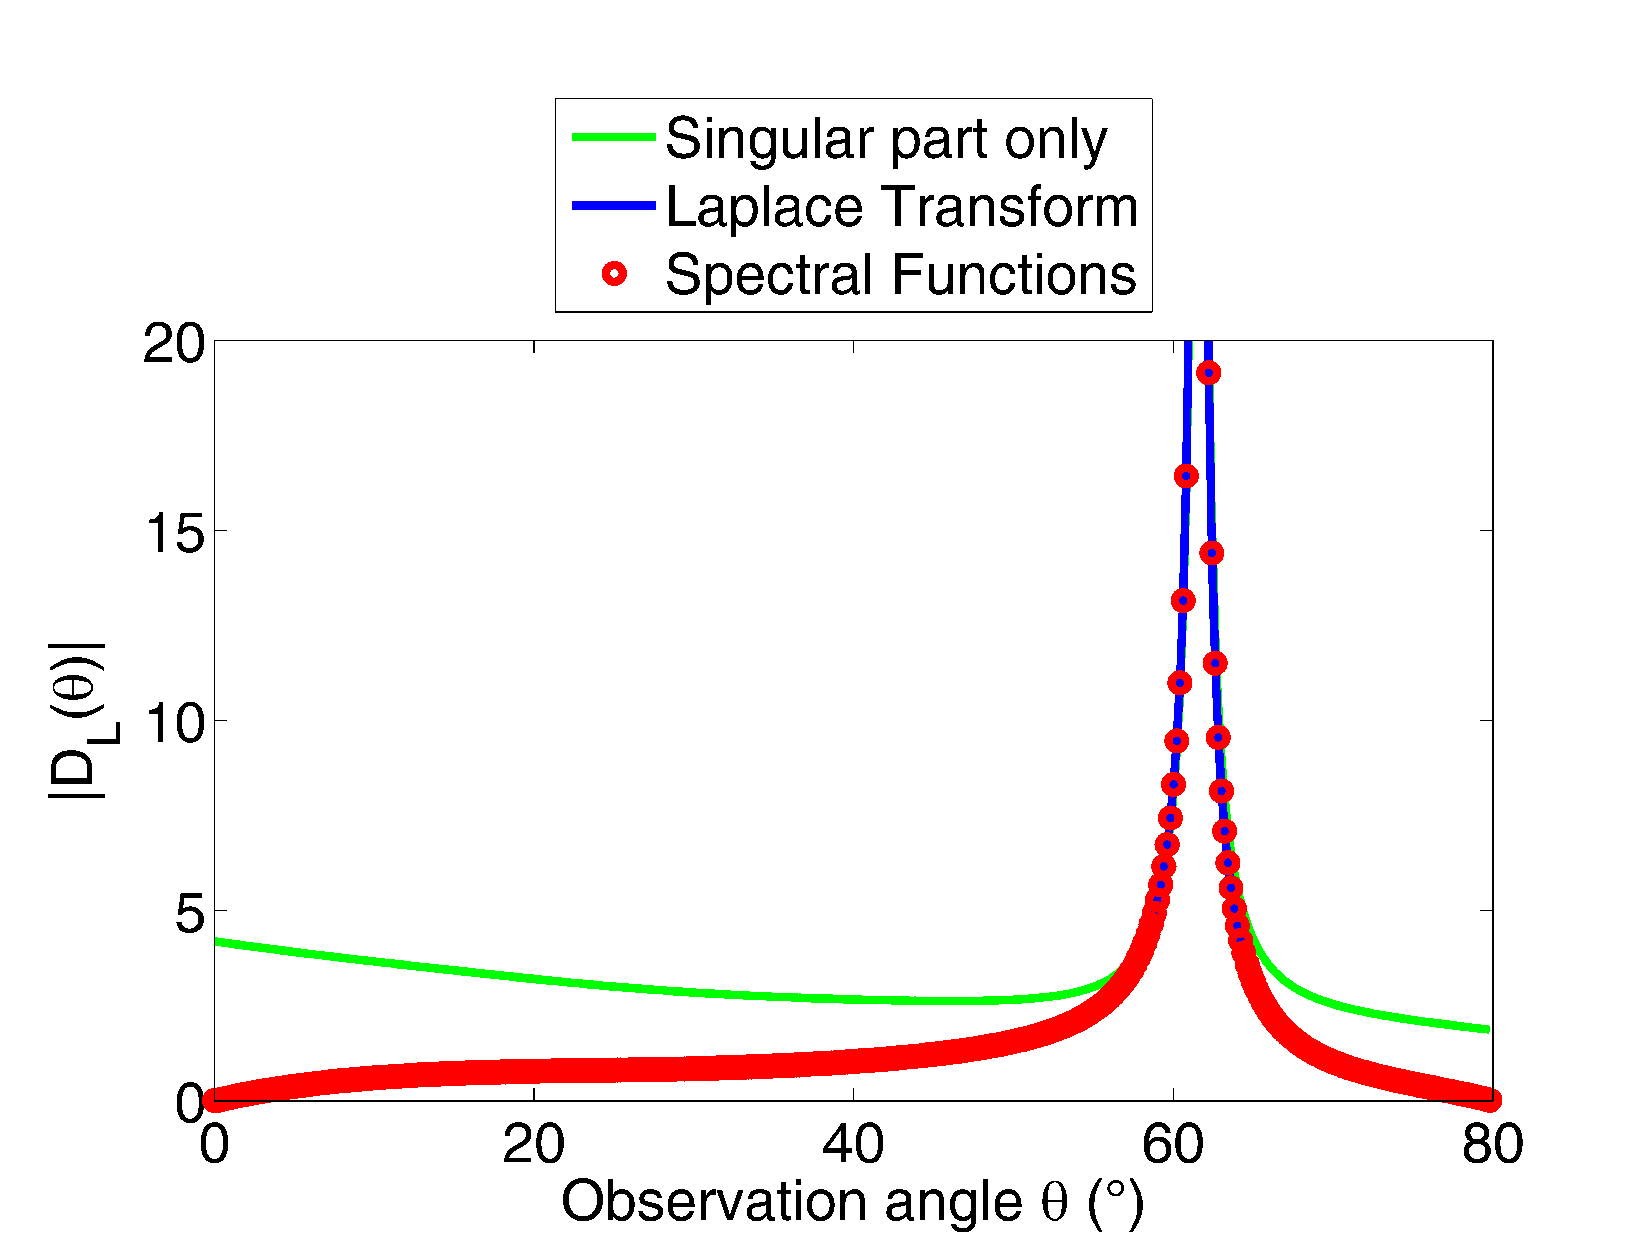
\includegraphics[width=\textwidth]{images/chapter3/Figure8c.pdf}
        \caption{Diffracted L wave and incident T wave}
    \end{subfigure}
    \begin{subfigure}[b]{0.44\textwidth}
        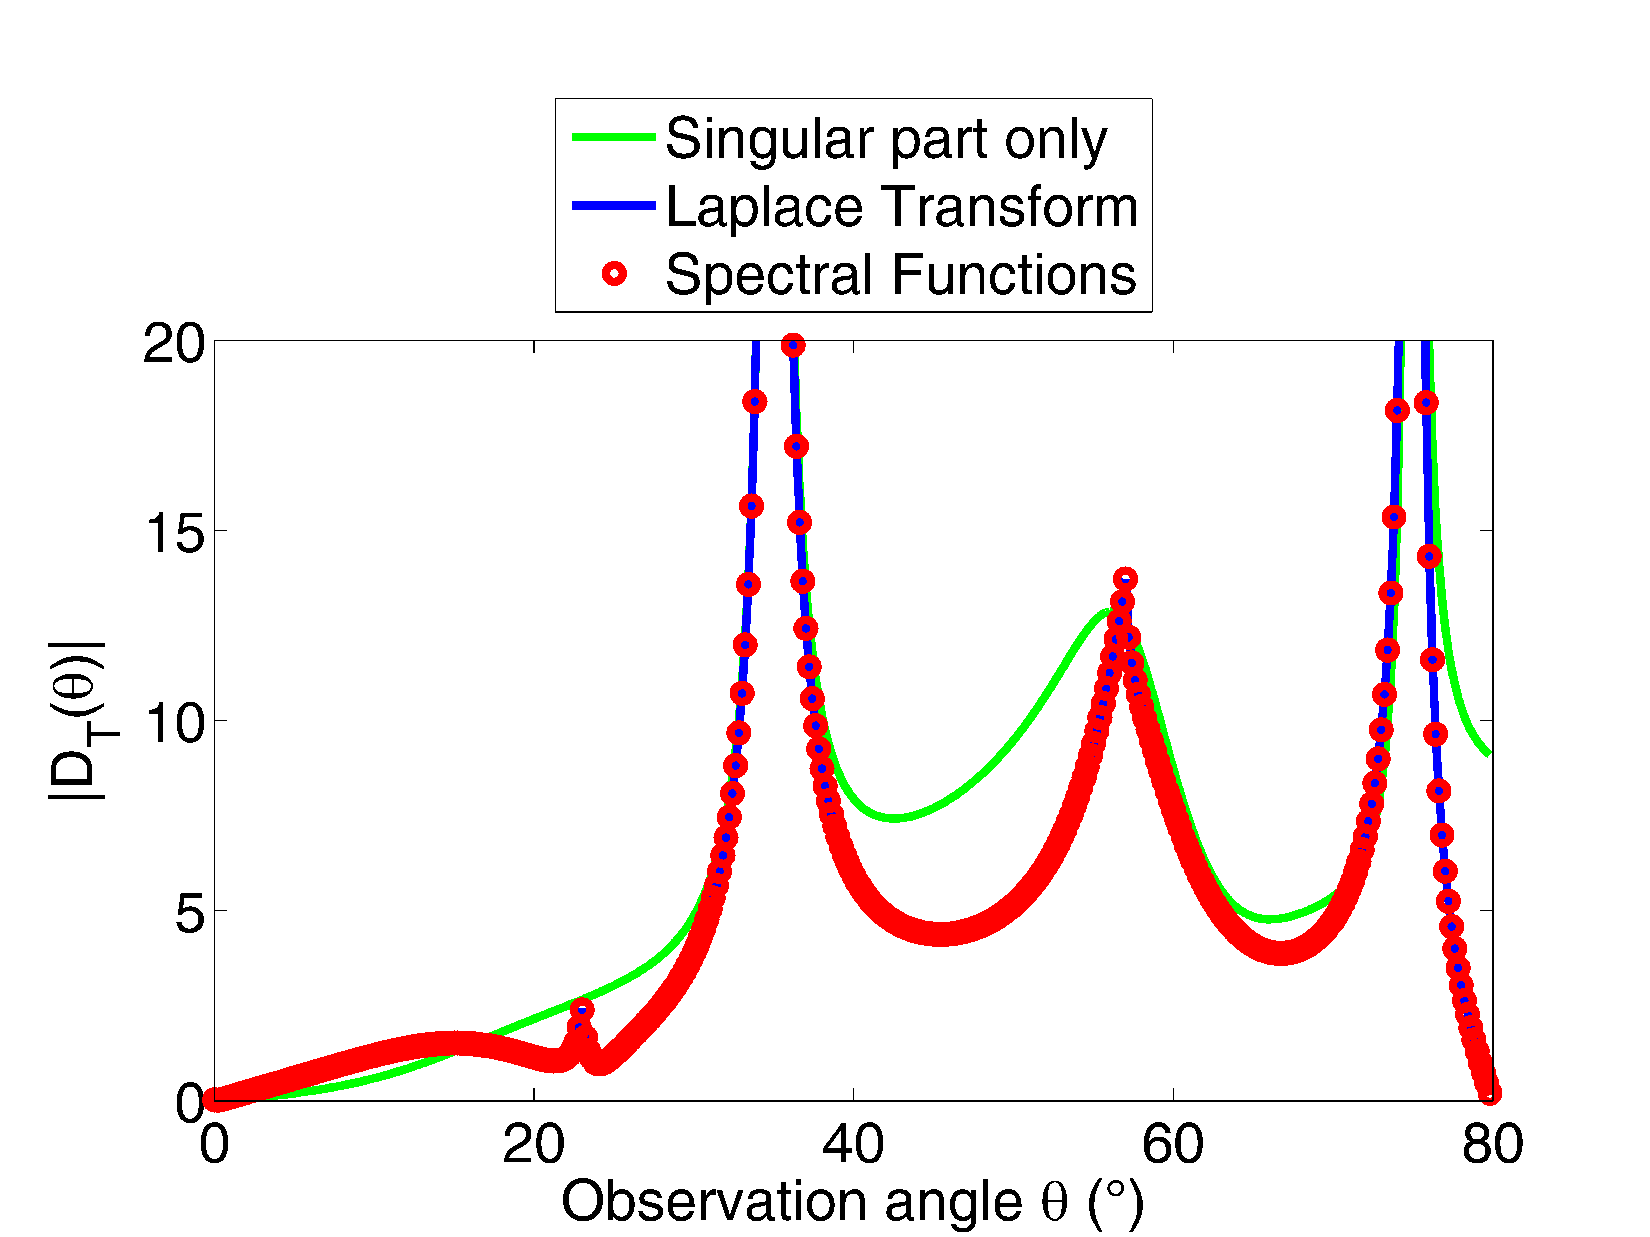
\includegraphics[width=\textwidth]{images/chapter3/Figure8d.pdf}
        \caption{Diffracted and incident T waves}
     \end{subfigure}
     \caption{Diffraction coefficients for $\varphi=80^o, \theta_{inc}=55^o$}
     \label{8055}
\end{figure}

\begin{figure}
\centering
    \begin{subfigure}[b]{0.44\textwidth}
        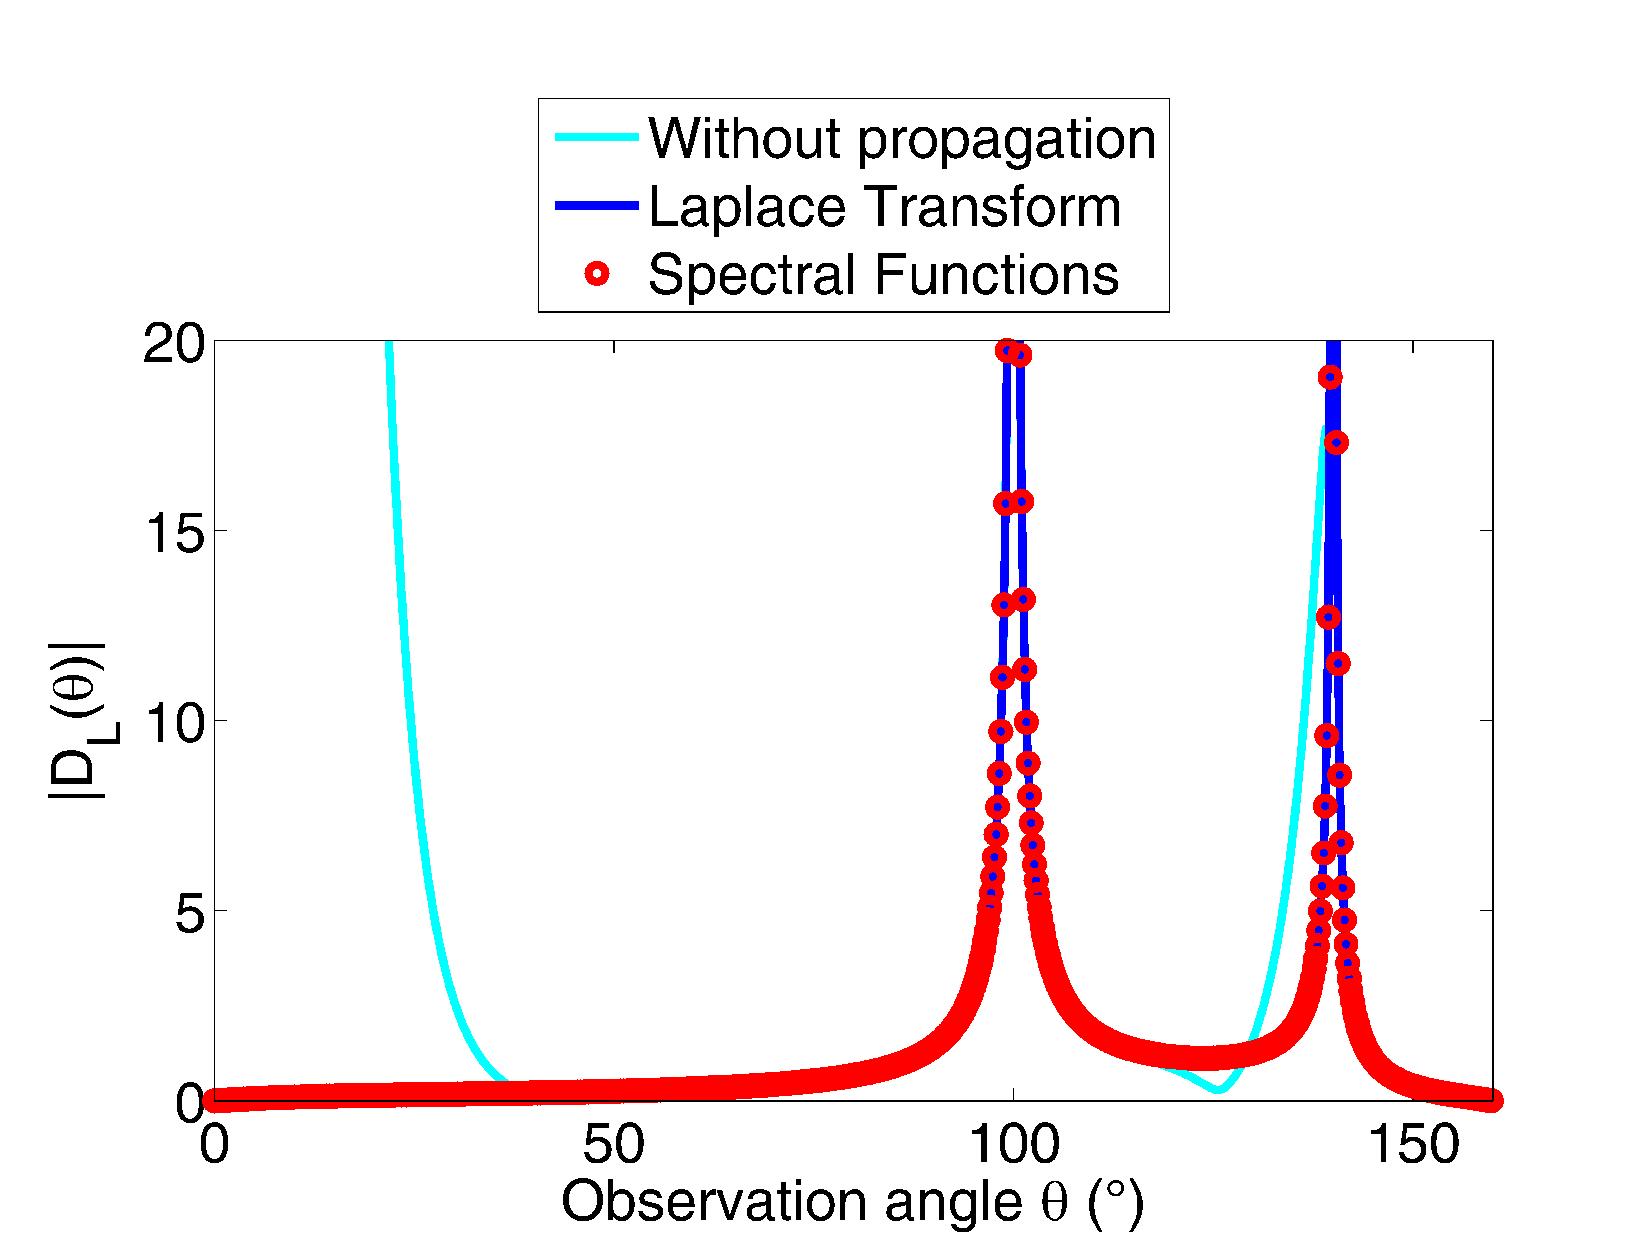
\includegraphics[width=\textwidth]{images/chapter3/Figure9a.pdf}
        \caption{Diffracted and incident L waves}
    \end{subfigure}  
    \begin{subfigure}[b]{0.44\textwidth}
        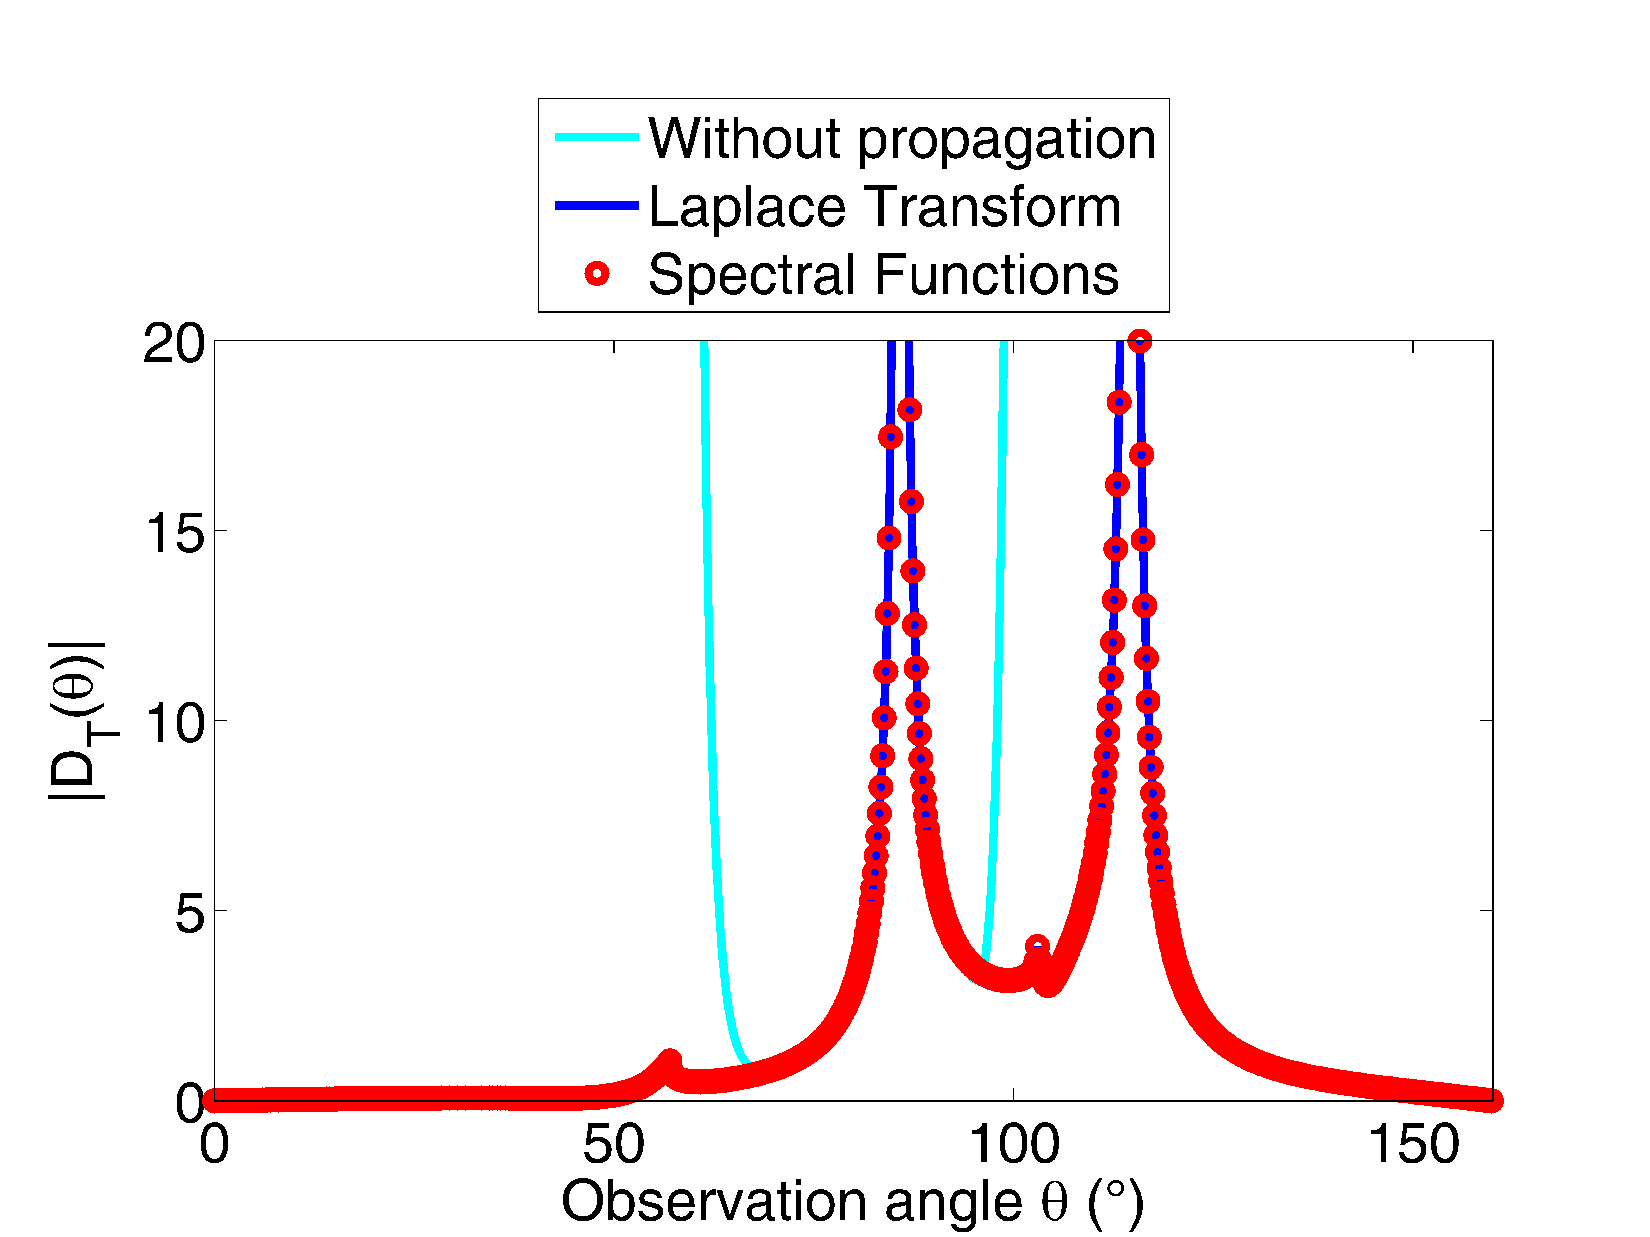
\includegraphics[width=\textwidth]{images/chapter3/Figure9b.pdf}
        \caption{Diffracted T wave and incident L wave}
     \end{subfigure} \\   
     \begin{subfigure}[b]{0.44\textwidth}
        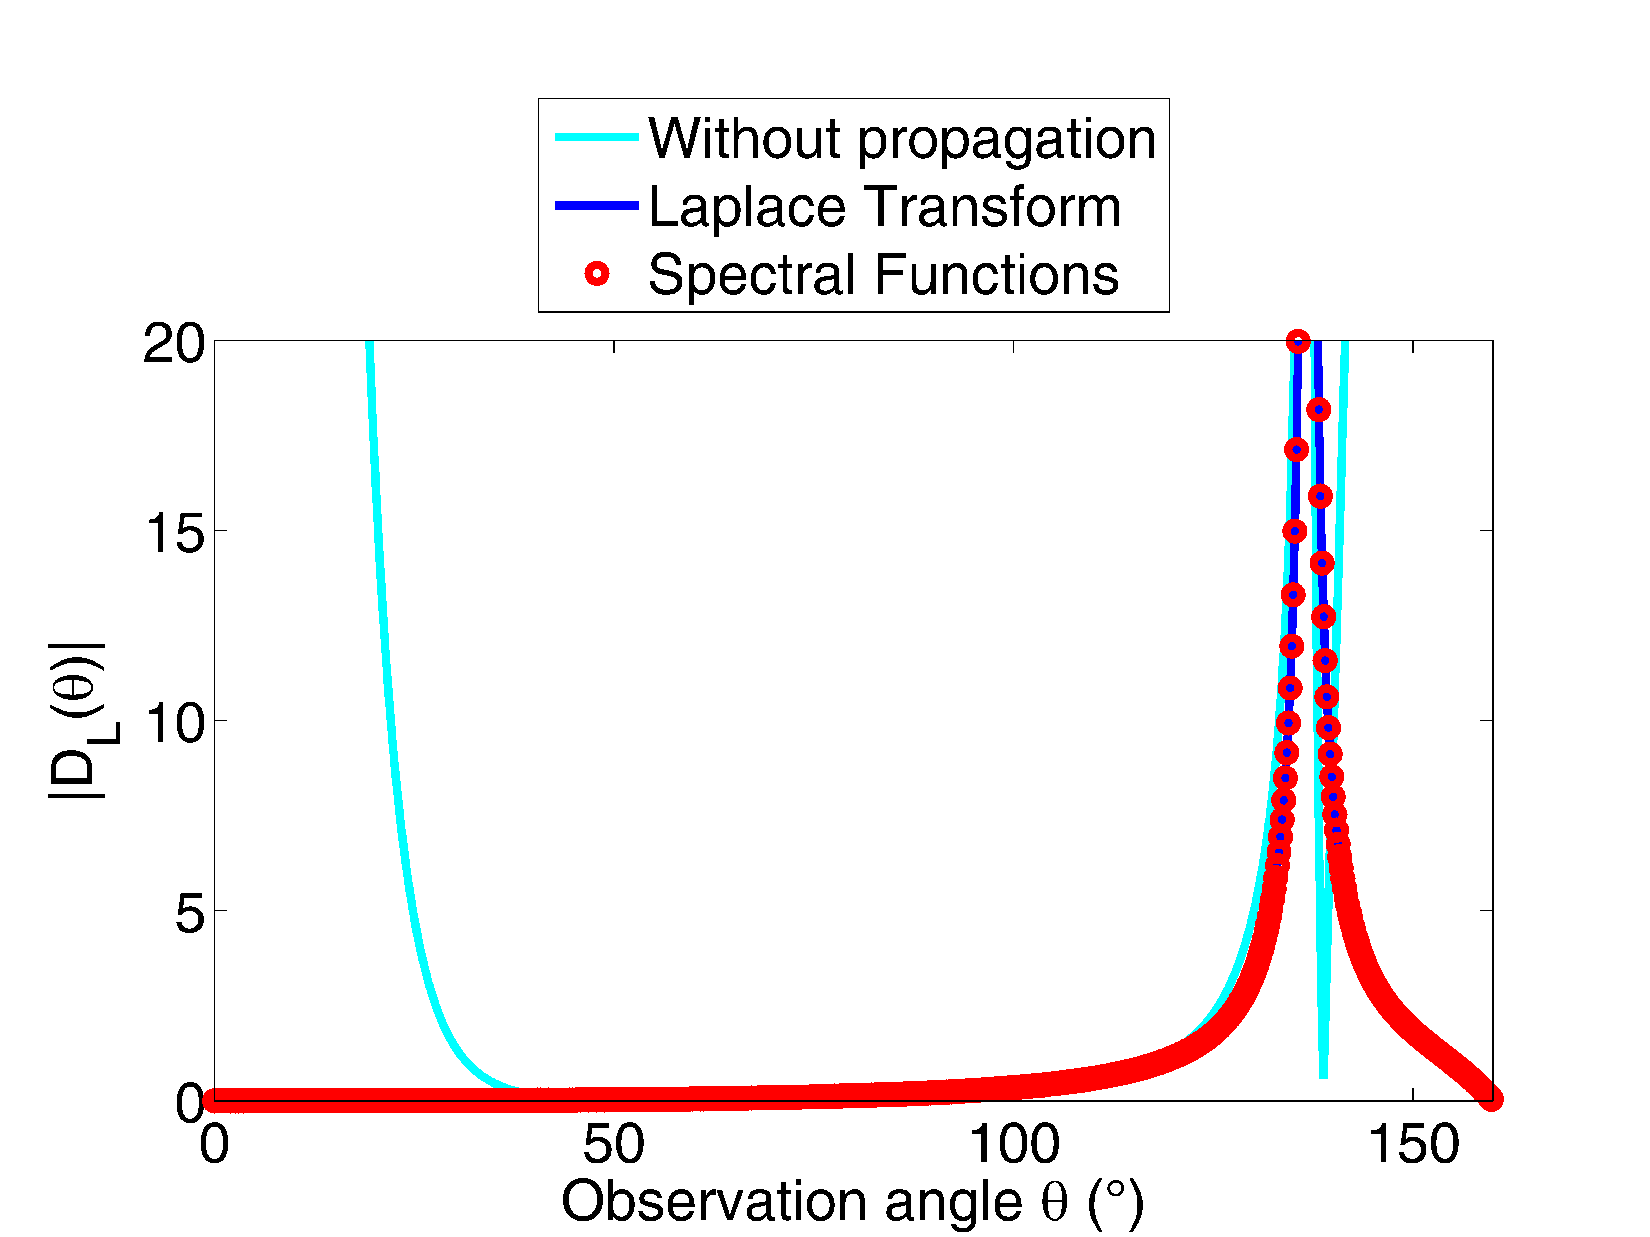
\includegraphics[width=\textwidth]{images/chapter3/Figure9c.pdf}
        \caption{Diffracted L wave and incident T wave}
    \end{subfigure}
    \begin{subfigure}[b]{0.44\textwidth}
        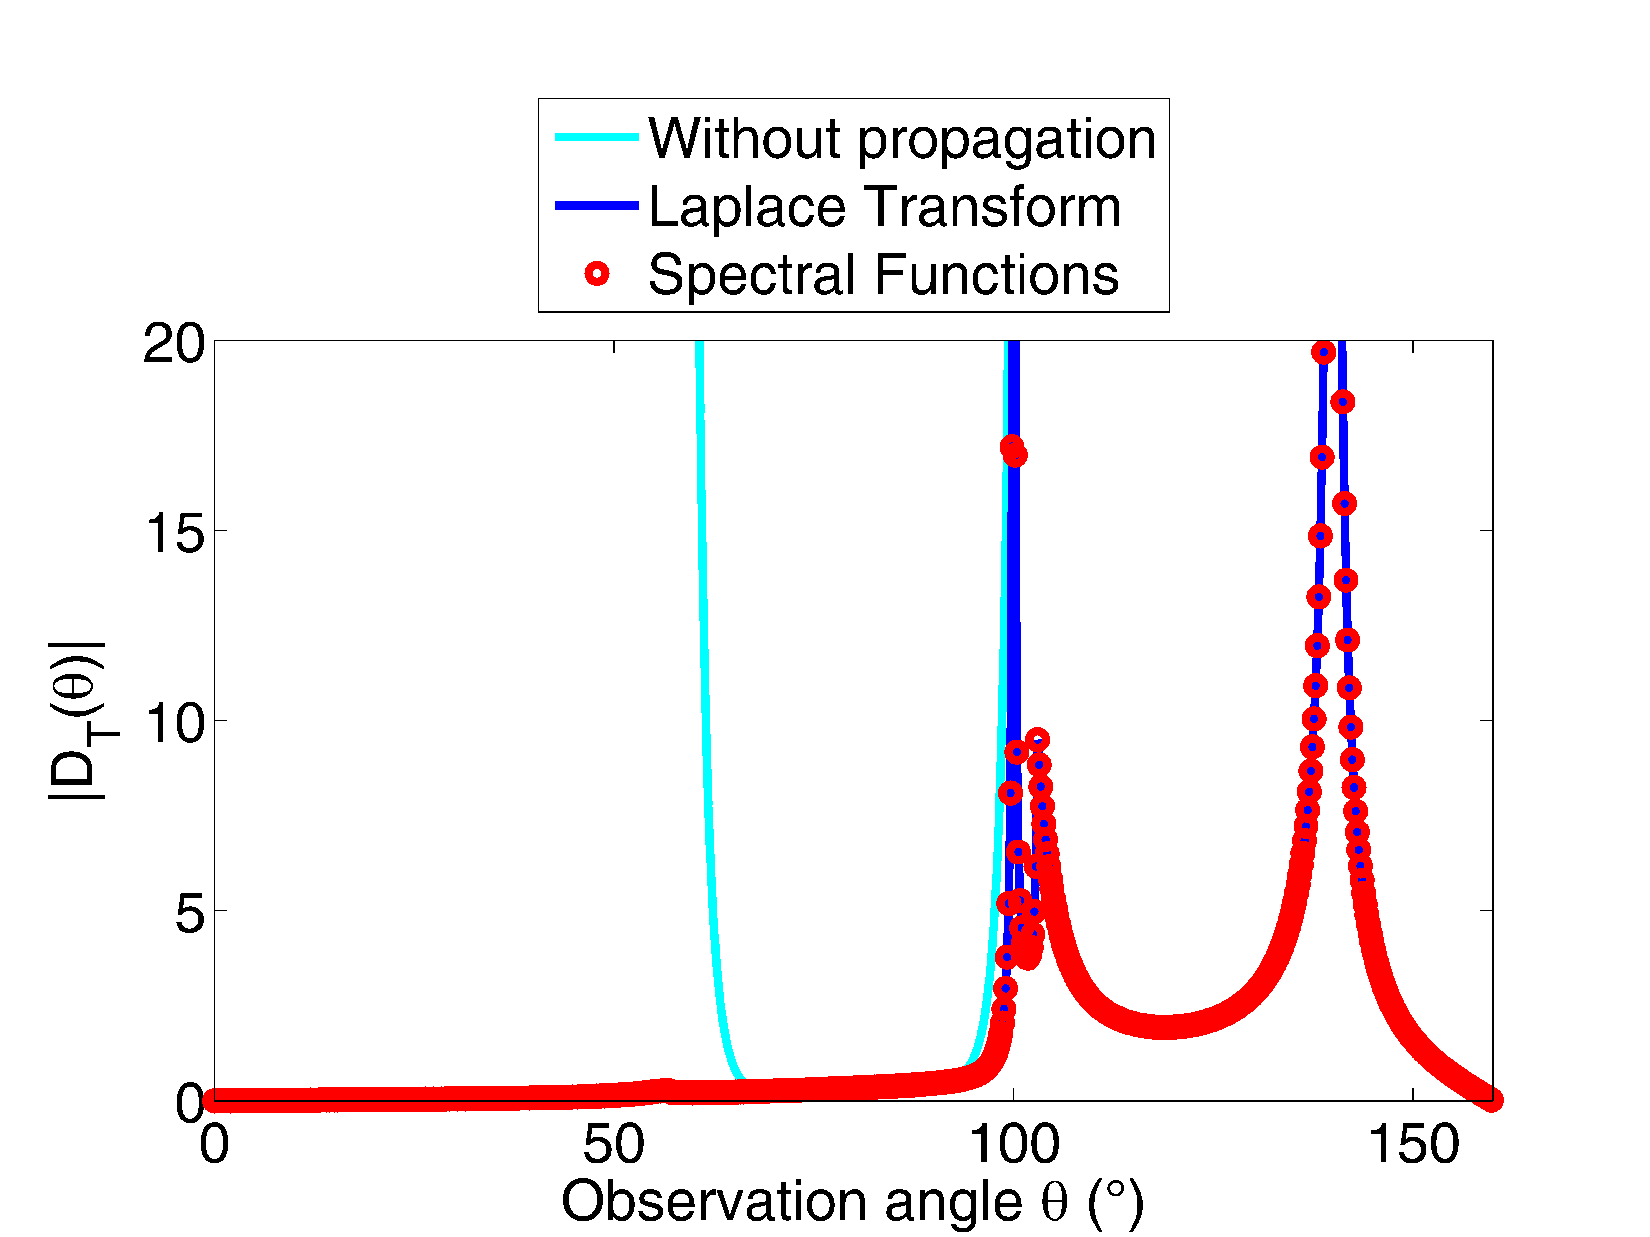
\includegraphics[width=\textwidth]{images/chapter3/Figure9d.pdf}
        \caption{Diffracted and incident T waves}
     \end{subfigure}
     \caption{Diffraction coefficients for $\varphi=160^o, \theta_{inc}=40^o$}
     \label{16040}
\end{figure}

For all of the tested configurations (different wedge and incidence angles), the results are conclusive. The results using the spectral functions method are extremely close to those obtained using the \acrshort{lt} code, which has been validated both numerically and experimentally \cite{GautesenFradkin, ChapmanBurch}. This constitutes a satisfying validation for wedge angles $\varphi \leq \pi$. Some additional numerical comparisons have been made in the next section for the case of a wedge of angle $\varphi>\pi$.

\subsection{For $\varphi>\pi$}
For wedge angles $\varphi \geq \pi$, the existing \acrshort{lt} code can not be used. Therefore, the spectral finite elements code of Imperiale et al. developed for the commercial software CIVA \cite{imperiale_ut_2016, imperiale_ut_2017} has been used as a reference solution for numerical validation purposes. The scattered wave fronts have been computed using this \acrfull{fe} method and the diffraction coefficients are extracted from these. The frequency of the incident wave is set to $f=1,0$MHz. The \acrshort{fe} computation box is visible on the snapshots in Fig.~\ref{snap}. The mesh size is $h=0,0432 \rm mm$ and the simulation time step is set to verify the \acrfull{cfl} stability condition ($\delta t=1,40963 \mu s$). The boundaries of the \acrshort{fe} computation box which correspond to the wedge edges are set to be stress-free boundaries and the other boundaries of the domain are \acrfull{pml}, which are absorbing boundaries used to mimic an infinite propagation domain.

The \acrshort{fe} code computes the reflected and diffracted wave field in the time-domain. The incident wave is a pulse with a plane wavefront and the value of the diffracted wave field is extracted along the cylindrical diffracted wavefront as detailed in the following. To do so, a snapshot is taken at a time where the diffracted wavefronts are located inside the \acrshort{fe} box but the furthest possible from the edge, in order for the far-field approximation to be applicable, whilst minimizing interferences that may occur from non-physical waves reflected from the borders of the \acrshort{fe} computation domain. These snapshots are presented in Fig.~\ref{snap} for two different propagation times. 

Fig.~\ref{snapLL} shows the snapshot used in the case of an L wave incident with an angle $\theta_{inc}=135^o$. The cylindrical wavefronts of the L (dLW) and T (dTW) waves diffracted from the wedge edge are visible, as well as the reflected L (rLW) and T (rTW) waves on each face of the wedge. Finally, Rayleigh waves (RW) propagating along each face of the wedge interfere with the diffracted T wave at the vicinity of the wedge faces for the chosen propagation time. 
Similarly, fig.~\ref{snapTL} shows the snapshot simulated in the case of a T wave incident with an angle $\theta_{inc}=135^o$. Once again, the cylindrical wavefronts of the L (dLW) and T (dTW) waves diffracted from the wedge edge are visible. In this case, there is no mode conversion and only reflected T waves (rTW) appear. Rayleigh waves (RW) which interfere with the diffracted T wave are also visible in this case and head waves (HW) are emanated from each face at the medium's longitudinal critical angle (for a steel/void interface, this angle is $\theta_c \approx 57^o$  inside steel). Some models have recently been proposed to mimic some head waves for half-plane scatterers \cite{PTDdarmon, FradkinDarmon}.

In order to extract diffraction coefficients from the \acrshort{fe} wave field, formula \eqref{defcoeffdiff} is used. The diffraction coefficient is deduced from the \acrshort{fe} wave field by :
\begin{equation}
D_{\beta}^{\alpha}(\theta)=\frac{v^{diff}_{\beta}(r\cos\theta,r\sin\theta)}{v_{inc}^{\alpha}(r\cos\theta,r\sin\theta)}e^{i\nu_{\beta}r}\sqrt{\nu_{\beta}r}
\label{FEextract}
\end{equation}
For each of these snapshots, the distance $r$ from the edge to the wavefront of the considered (L or T) edge diffracted wave is computed using the wave velocity and the chosen propagation time, and the norm of the field $||v^{diff}_{\beta}||$ is extracted on the point of the \acrshort{fe} mesh which is closest to the wavefront for each observation angle $\theta$. The diffraction coefficient is finally computed using formula \eqref{FEextract}. The results are shown in Fig.~\ref{270135}.

\begin{figure}
\centering
    \begin{subfigure}[b]{0.44\textwidth}
        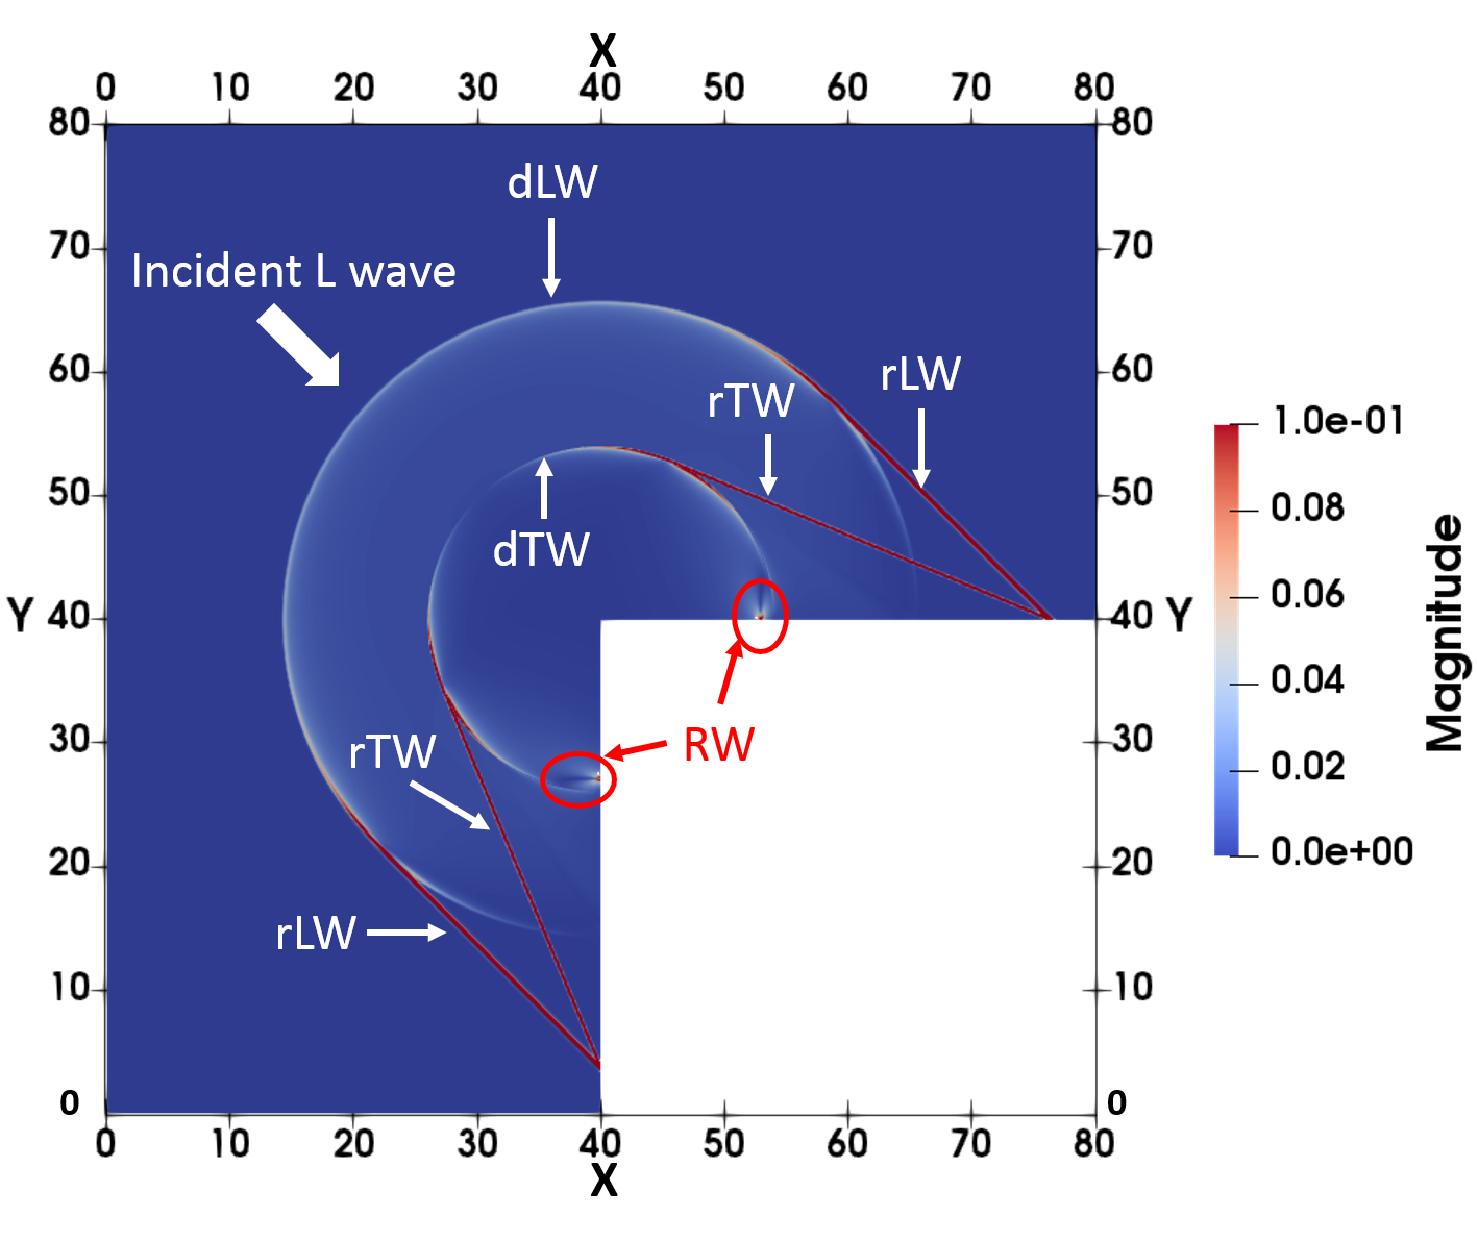
\includegraphics[width=\textwidth]{images/chapter3/Figure10a.pdf}
        \caption{Incident L wave, $t=5ms$.}
        \label{snapLL}
    \end{subfigure}  
    ~
     \begin{subfigure}[b]{0.44\textwidth}
        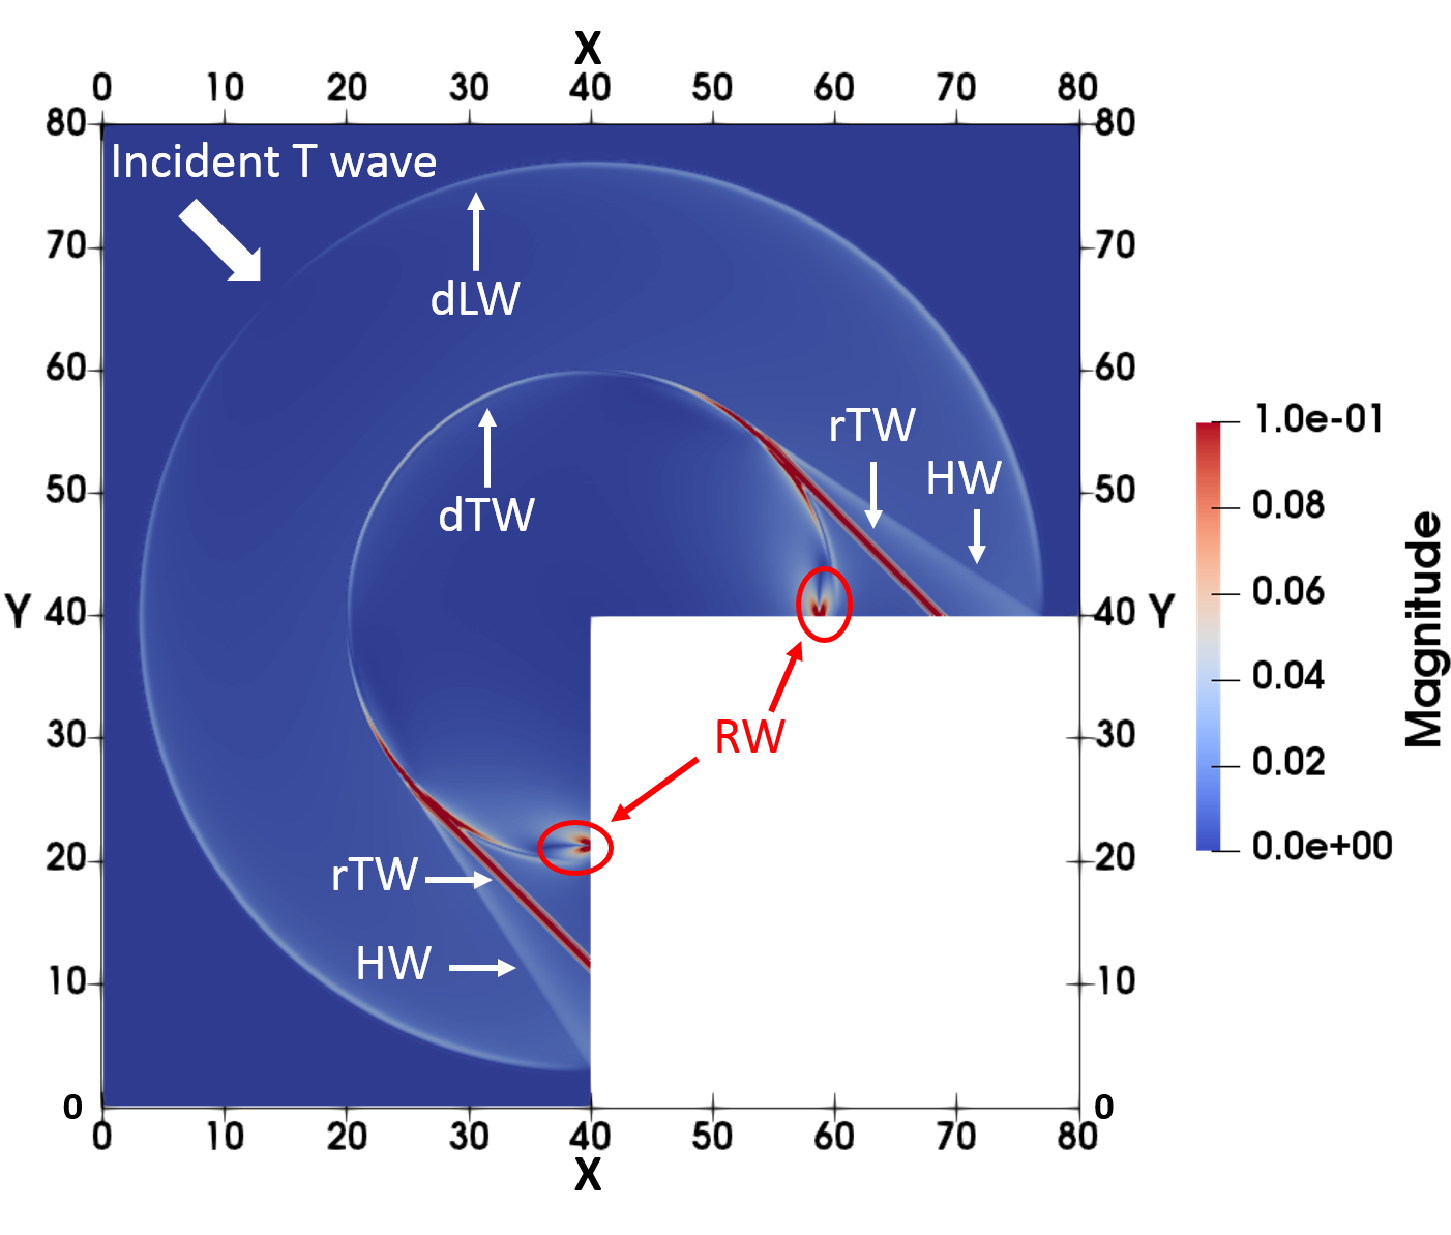
\includegraphics[width=\textwidth]{images/chapter3/Figure10b.pdf}
        \caption{Incident T wave, $t=6,5ms$. }
        \label{snapTL}
    \end{subfigure}
     \caption{Finite elements snapshots. Distances are given in millimeters. }
     \label{snap}
\end{figure}

\begin{figure}%[H]
\centering
    \begin{subfigure}[b]{0.44\textwidth}
        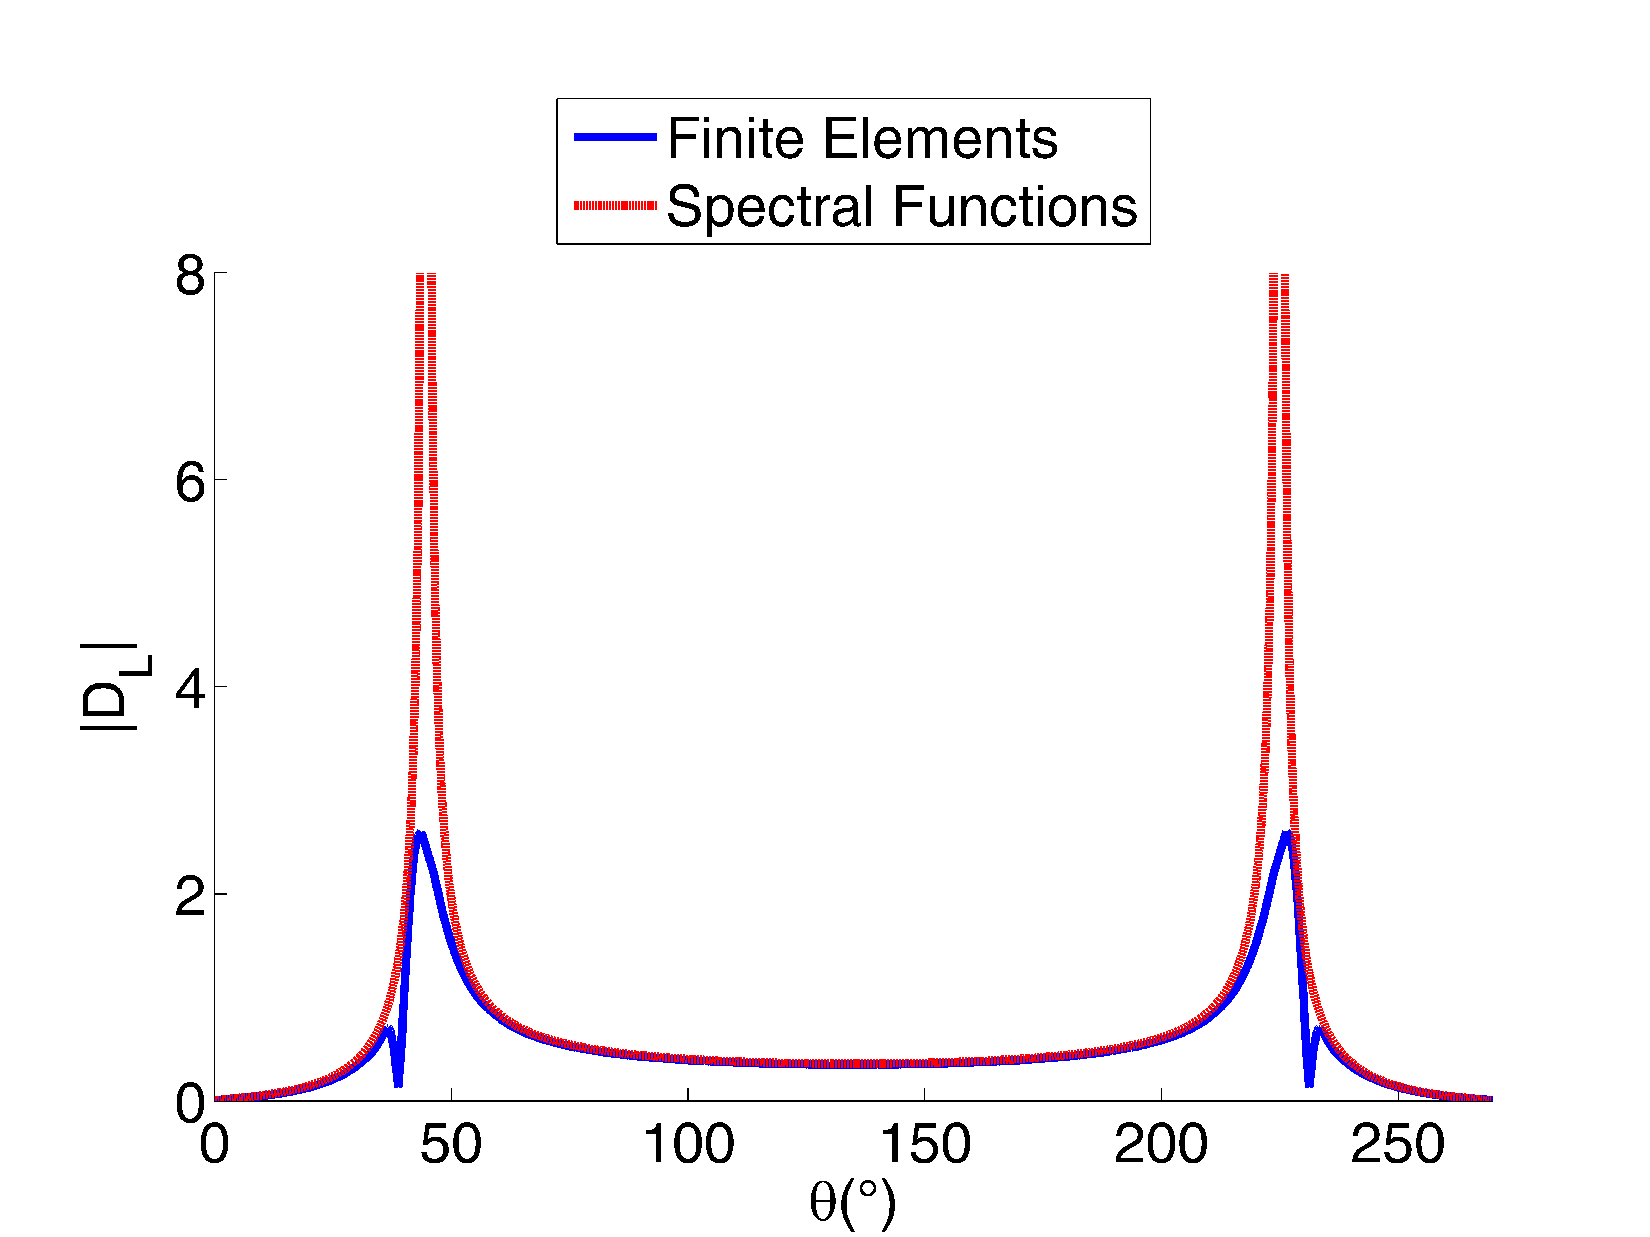
\includegraphics[width=\textwidth]{images/chapter3/Figure11a.pdf}
        \caption{Diffracted and incident L waves. $r=25,6 \rm mm$.}
        \label{DLL}
    \end{subfigure}  
    \begin{subfigure}[b]{0.44\textwidth}
        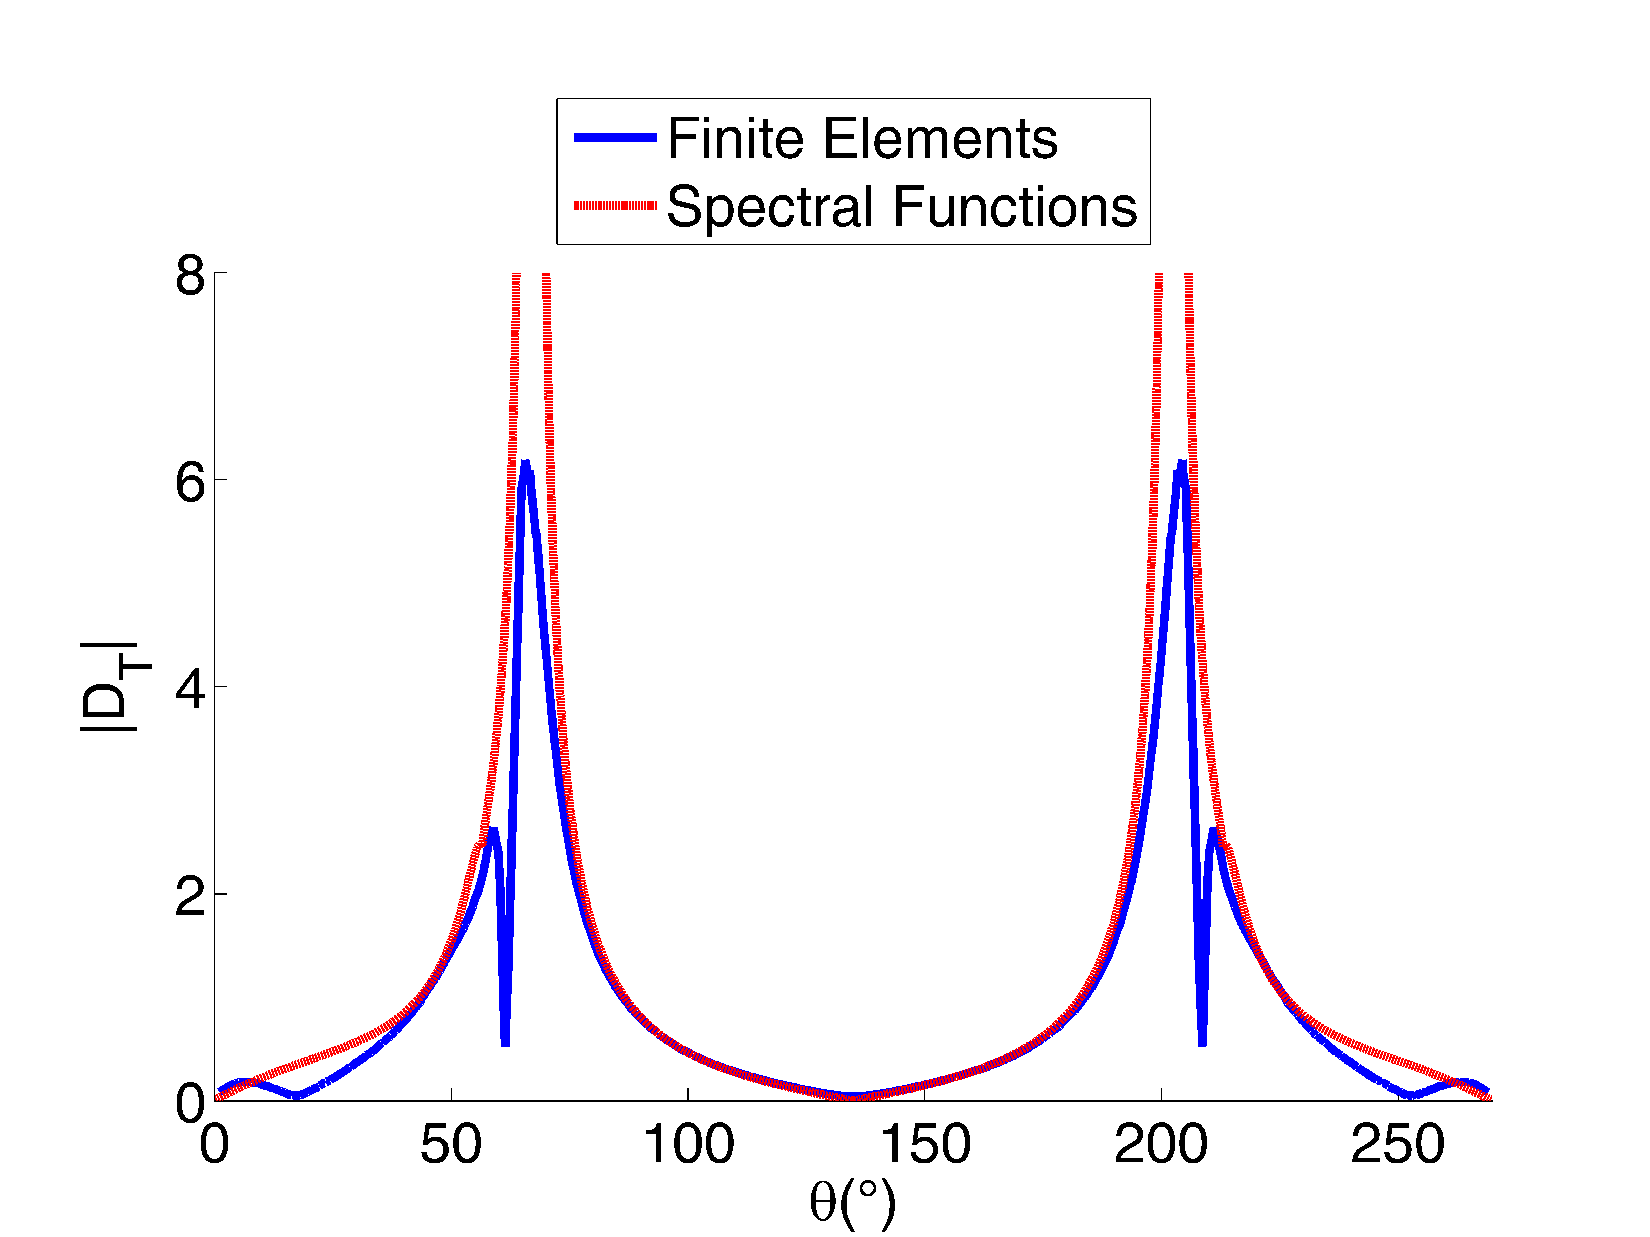
\includegraphics[width=\textwidth]{images/chapter3/Figure11b.pdf}
        \caption{Diffracted T wave and incident L wave. $r=13,9 \rm mm$.}
        \label{DLT}
     \end{subfigure}   
     \begin{subfigure}[b]{0.44\textwidth}
        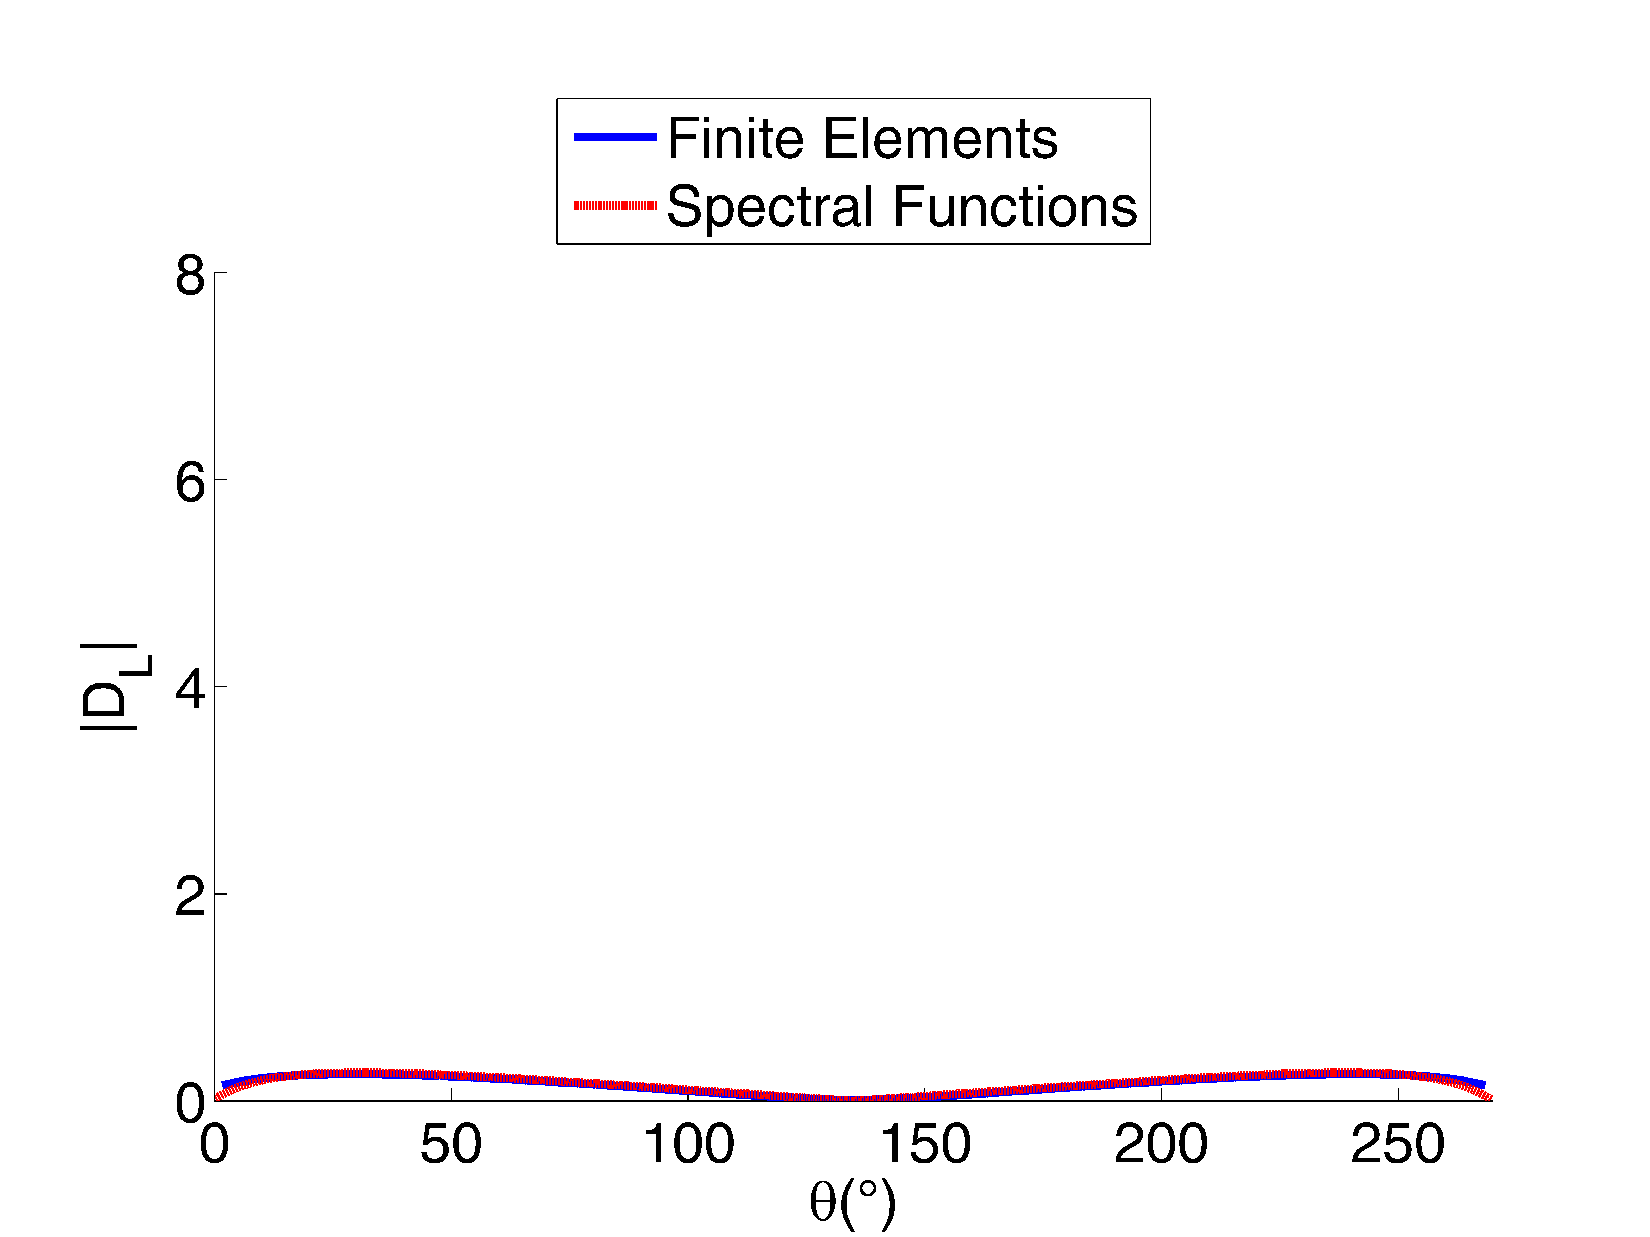
\includegraphics[width=\textwidth]{images/chapter3/Figure11c.pdf}
        \caption{Diffracted L wave and incident T wave. $r=36,5 \rm mm$.}
        \label{DTL}
    \end{subfigure}
    \begin{subfigure}[b]{0.44\textwidth}
        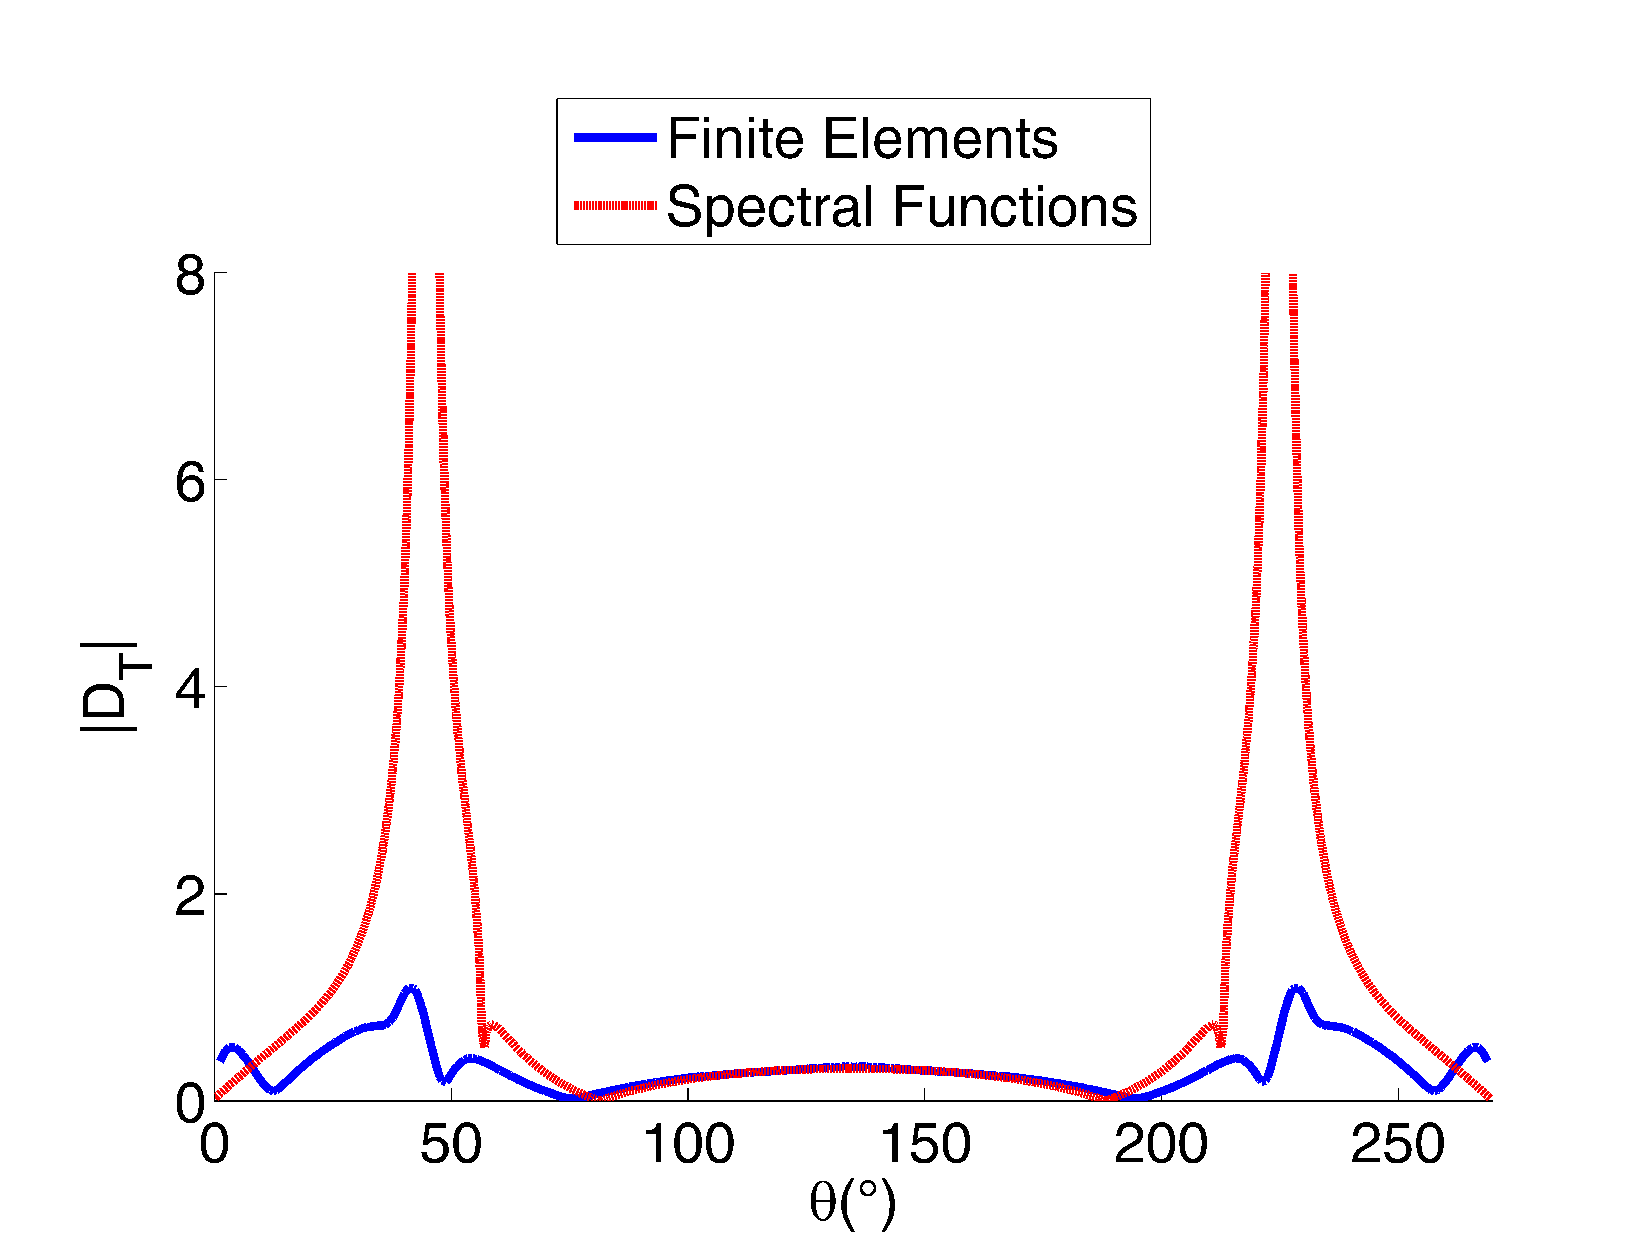
\includegraphics[width=\textwidth]{images/chapter3/Figure11d.pdf}
        \caption{Diffracted and incident T waves. $r=19,8 \rm mm$.}
        \label{DTT}
     \end{subfigure}
     \caption{Diffraction coefficients for $\varphi=270^o, \theta_{inc}=135^o$}
     \label{270135}
\end{figure}

Fig.~\ref{270135} shows the absolute value of the diffraction coefficients, obtained for a wedge of angle $\varphi=270^o$ illuminated by a wave incident with an angle $\theta_{inc}=135^o$, plotted with respect to the observation angle. The blue line is the diffraction coefficient extracted from the finite elements wave front and the dashed red line is the result obtained from the \acrshort{sf} code. 

Overall, both lines overlap quite well, though some differences are observed. The most obvious difference between the plots is that the \acrshort{fe} diffraction coefficient always remains finite, whereas the \acrshort{sf} diffraction coefficient possesses poles (except for Fig.~\ref{DLT} where there are no reflected L waves). This is due to the fact that the \acrshort{sf} diffraction coefficient is a \acrshort{gtd}-like coefficient obtained from a far-field asymptotic evaluation \eqref{defcoeffdiff} and it diverges at shadow boundaries \cite{GTD,Audrey}. The \acrshort{fe} code notably computes the reflected waves as well as the diffracted waves in angular regions surrounding the reflected poles ; consequently, reflected waves give a contribution to the \acrshort{fe} diffraction coefficient. The contribution of these reflected plane waves to the \acrshort{fe} diffraction coefficient, computed using \eqref{FEextract}, grows with the distance $r$, since it contains the factor $\sqrt{\nu_{\beta}r}$ and the reflected plane waves have theoretically constant amplitudes. Interference between these plane reflected waves and the cylindrical diffracted waves explain the spikes that can be observed in the \acrshort{fe} diffraction coefficients, near the poles of the \acrshort{gtd} diffraction coefficients in Figs.~\ref{DLL}, \ref{DLT} and \ref{DTT}. Some uniform methods have been proposed to handle the divergence of \acrshort{gtd} diffraction coefficients and build a spatially uniform total field and some of them have been applied to elastodynamic half-plane scattering \cite{Audrey, Zernov, PTDdarmon}.

On Figs.~\ref{DLT} and \ref{DTT} for diffracted T waves, the \acrshort{fe} diffraction coefficient seems to have a slightly different behavior near the wedge edges than the \acrshort{sf} diffraction coefficients. Since this discrepancy is only visible in the T diffraction coefficient, it seems unlikely that it is due to the branch points at angles $\theta=0$ and $\theta=\varphi$ mentioned in section \ref{farfield}, as these branch points would affect both L and T diffracted waves. The observed discrepancy is more probably due to interference of the diffracted T wavefront with the Rayleigh waves observed on Figs.~\ref{snapLL} and \ref{snapTL}, which modifies the observed \acrshort{fe} field along the diffracted T wavefront.

Away from shadow boundaries (where the non-uniform \acrshort{sf} code diverges) and domain borders i.e. in regions where diffracted waves do not interfere with other waves and where the \acrshort{sf} asymptotic evaluation is theoretically valid, the \acrshort{fe} and \acrshort{sf} codes give very similar results. 

\section{Experimental validation}
The \acrshort{lt} code used to validate the \acrshort{sf} method for wedge angles lower than $\pi$ has been validated experimentally by Chapman et al. \cite{ChapmanBurch}. Their experimental set-up is thoroughly described in \cite{ChapmanBurch} and will only be summarized here. The results of their experimental measurements will be used to validate the \acrshort{sf} code experimentally.

\begin{figure}[h!]
\centering
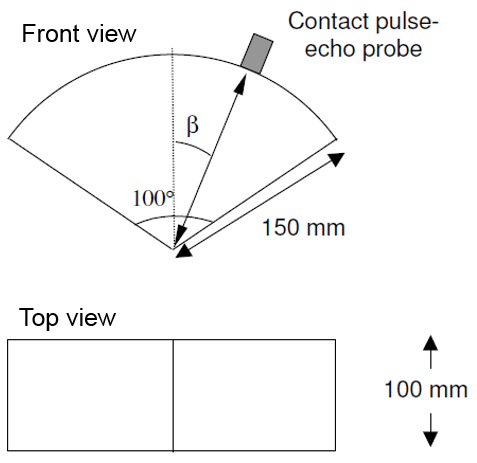
\includegraphics[scale=0.8]{images/chapter3/wedge_schema.png}
\caption{(Reproduced from \cite{ChapmanBurch}) Front and Top view of the wedge inspected in pulse-echo configuration.}
\label{C3:wedge_schema}
\end{figure}

Two isotropic ferritic steel ($c_L=5800\,m.s^{-1}, \; c_T=3230\,m.s^{-1}$) cylindrical sectors of radius 150mm, thickness 100mm wedges and of angles $\varphi=80^o$ and $\varphi=100^o$ are inspected in pulse-echo configuration, meaning that the emitting transducer is also the receiving transducer. In terms of the diffraction coefficient, this means that the observation angle is equal to the incidence angle.

\begin{figure}[h!]
\centering
    \begin{subfigure}[b]{0.45\textwidth}
        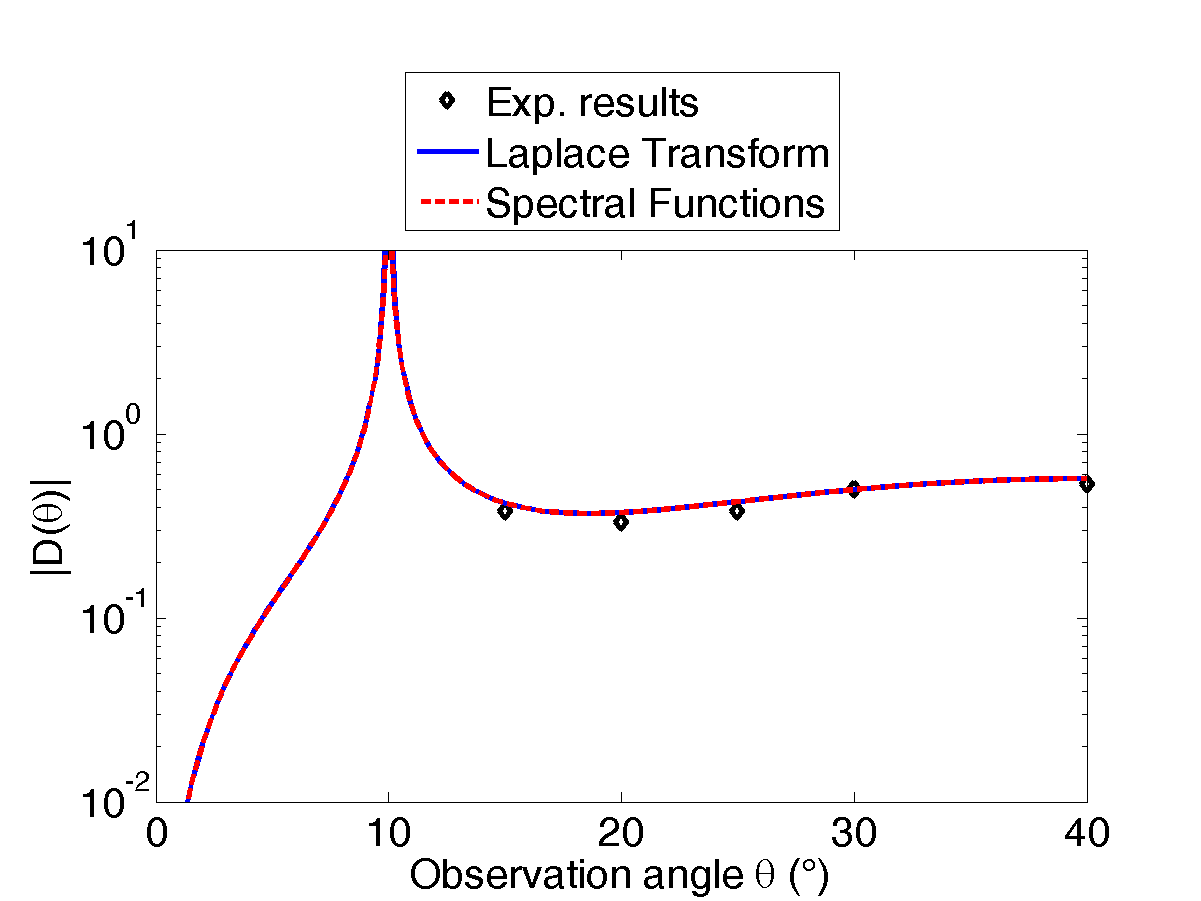
\includegraphics[width=\textwidth]{images/chapter3/Retrodiff_D_80_LL.png}
        \caption{Incident and diffracted L wave, $\varphi=80^o$.}
        \label{C3:DLL80}
    \end{subfigure}
    \hfill  
    \begin{subfigure}[b]{0.45\textwidth}
        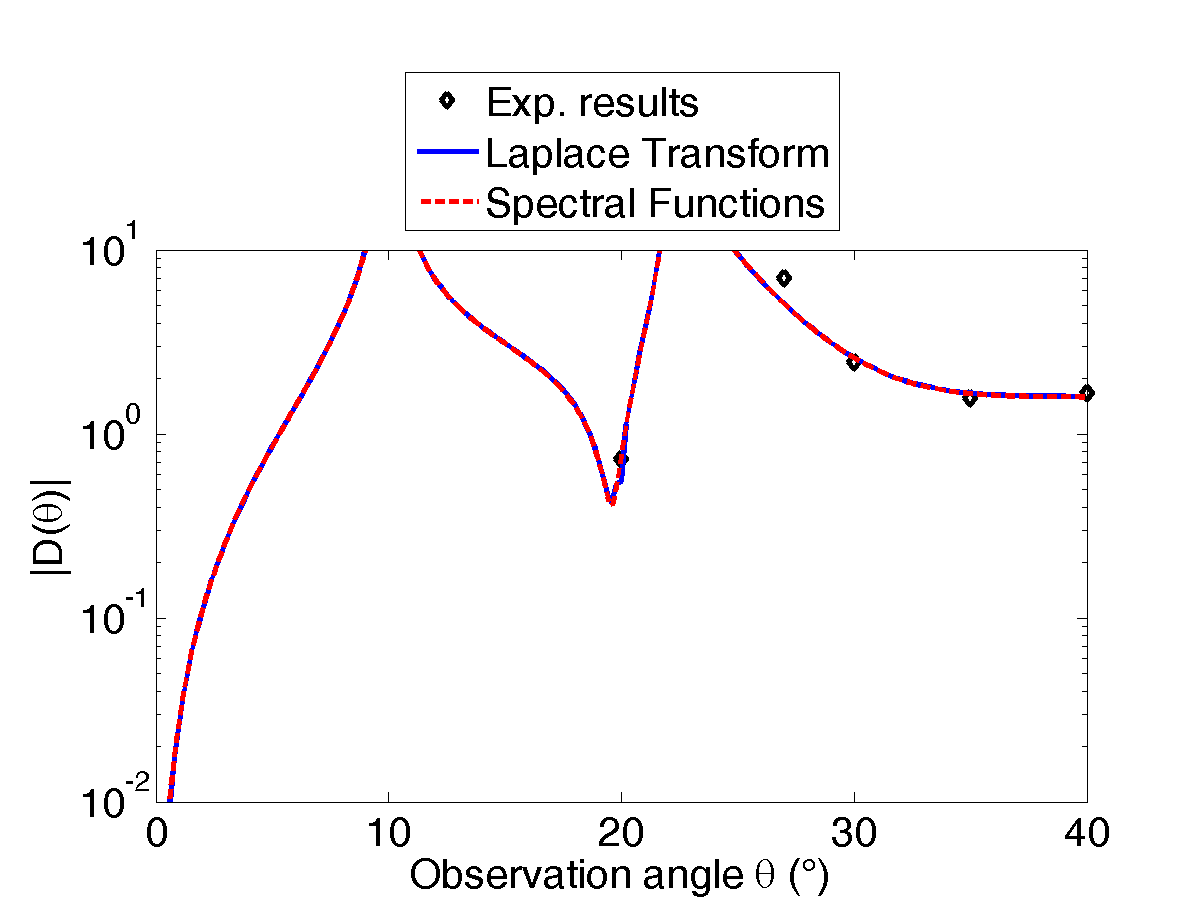
\includegraphics[width=\textwidth]{images/chapter3/Retrodiff_D_80_TT.png}
        \caption{Incident and diffracted T wave, $\varphi=80^o$.}
        \label{C3:DTT80}
     \end{subfigure} %\\  
%     \begin{subfigure}[b]{0.45\textwidth}
%        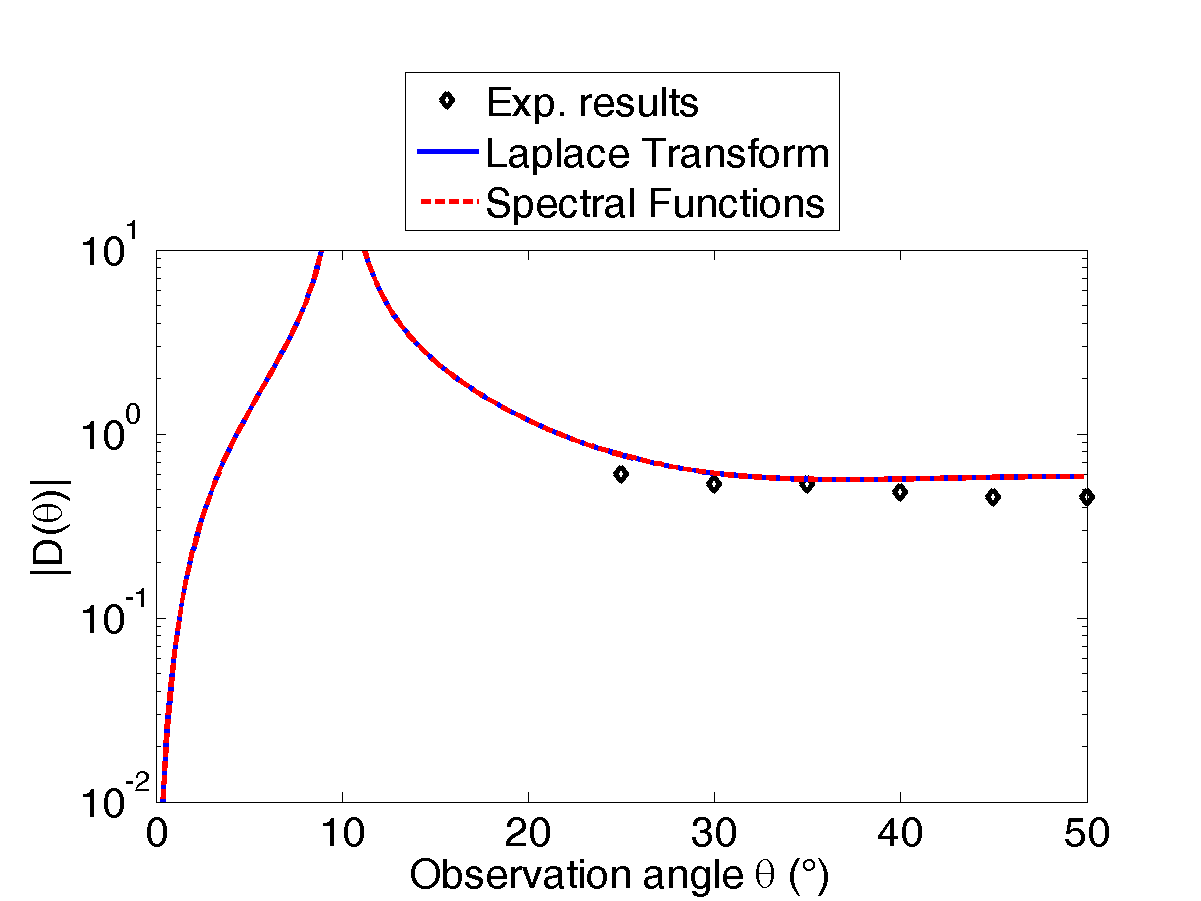
\includegraphics[width=\textwidth]{images/chapter3/Retrodiff_D_100_LL.png}
%        \caption{Incident and diffracted L wave, $\varphi=100^o$.}
%        \label{C3:DLL100}
%    \end{subfigure}
    \hfill
    \begin{subfigure}[b]{0.45\textwidth}
        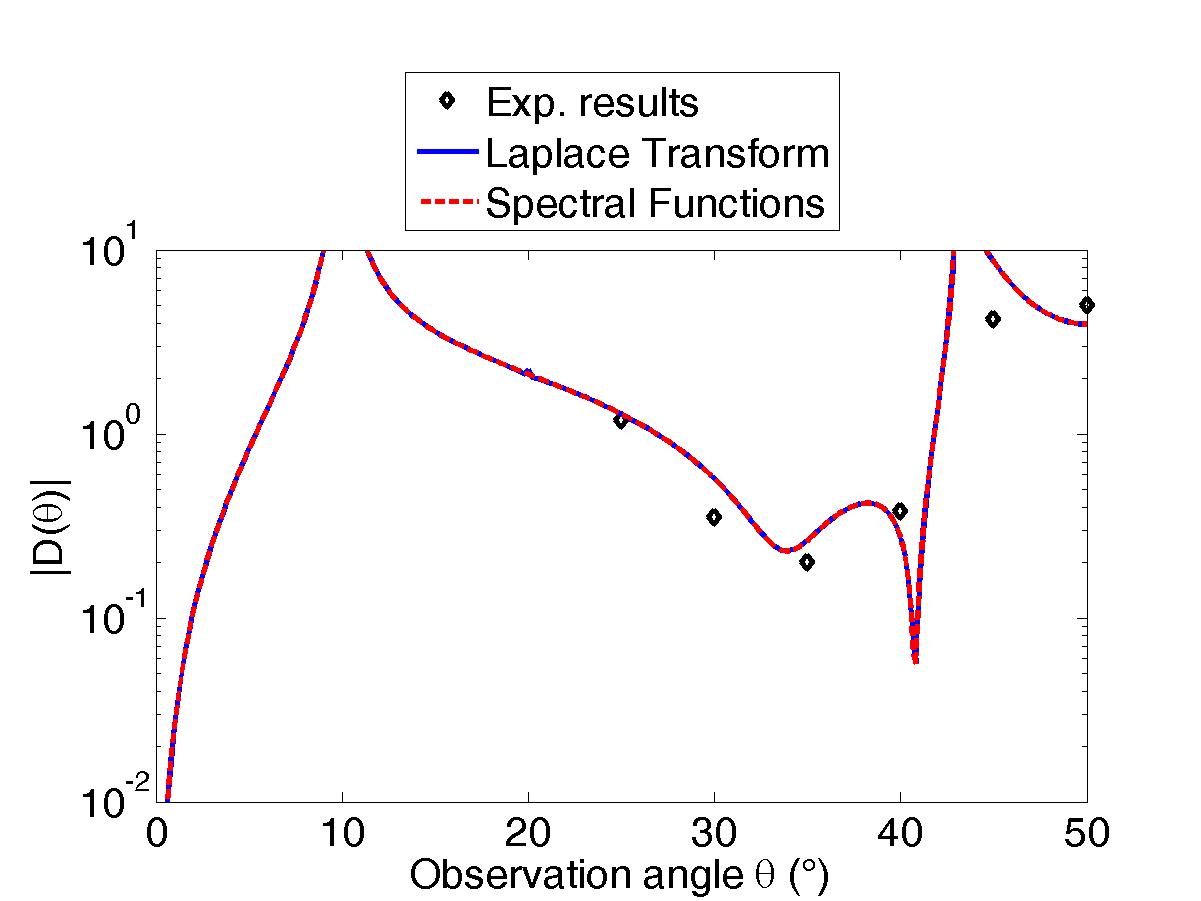
\includegraphics[width=\textwidth]{images/chapter3/Retrodiff_D_100_TT.png}
        \caption{Incident and diffracted T wave, $\varphi=100^o$.}
        \label{C3:DTT100}
     \end{subfigure}
     \caption{Backscattering diffraction coefficients for wedges $\varphi=80^o$ and $\varphi=100^o$.}
     \label{C3:expcoeffs}
\end{figure}

The inspections have been done at frequencies 2MHz and 5MHz to check that the diffraction coefficients do not depend on the frequency.  The experimental set-up is shown in Fig.~\ref{C3:wedge_schema}. Since the diffraction coefficients measured at both frequencies are identical, only the results obtained at 2MHz are presented here. Fig.~\ref{C3:expcoeffs} presents the comparison between the backscattering coefficients computed using the \acrshort{lt} code, the coefficients computed using the \acrshort{sf} code and the values measured experimentally presented in \cite{ChapmanBurch}.

Figs.~\ref{C3:DLL80} and \ref{C3:DTT80} show the absolute values of the L and T backscattering diffraction coefficients respectively, for a wedge of angle $\varphi=80^o$. Figs~\ref{C3:DLL100} and \ref{C3:DTT100} show the absolute values of the L and T backscattering diffraction coefficients respectively, for a wedge of angle $\varphi=100^o$. In each of these figures, the full blue line represents the results obtained using the \acrshort{lt} diffraction coefficients, the dashed red line represents the results obtained using the \acrshort{sf} diffraction coefficients and the black diamonds represent the results measured experimentally.

In each of the tested configurations, the results are conclusive. There is a very good agreement between the experimental measurements and numerical results, thus providing and additional validation for the \acrshort{sf} code.

\section*{Conclusion}
The spectral functions method for modeling the diffraction of an elastic wave by a stress-free wedge is presented here. It extends the region of validity of previously existing semi-analytical methods for high-frequency computation to all wedge angles. The numerical aspects of the computation are fully detailed and the diffraction coefficient obtained using this method has been compared to the one obtained using the Laplace Transform (LT) code in the case of a wedge angle lower than $\pi$, and to a spectral finite elements code in the case of a wedge angle higher than $\pi$. 
When compared to the LT semi-analytical computation method for wedge angles lower than $\pi$, the spectral functions code gives excellent results. For wedge angles higher than $\pi$, a finite elements code is used for validation and the spectral functions method gives very good results in the domain of validity of the far-field asymptotic model. Finally, the results of the code are compared to experimental measurement, and the results are also good.

%
% Quatrième chapitre
\chapter[][3D Elastic Case]{The spectral functions method for 3D elastic wave diffraction by a stress-free wedge}
\label{chap-3D}

\section*{Introduction}

In the previous chapters of this manuscript, the spectral functions method has been presented in the case of an acoustic wave incident on a wedge with Dirichlet or Neumann boundaries and in the case of an elastic wave incident on a stress-free wedge. Both of these problems have been treated in the case of 2D incidences, meaning that the incident ray is in the plane normal to the wedge edge. In this chapter, we will extend the spectral functions method to the case of 3D incidences. This extension will be done for elastic waves incident on stress-free wedges and it will be shown that the code developed for the elastic case can be applied to the case of an acoustic wave incident on a wedge with Dirichlet boundary conditions, as well as to the 2D elastic problem.

The problem of 3D wedge diffraction has been studied over the past century in acoustics, electromagnetics and elastodynamics. The problem was introduced by Sommerfeld \cite{Sommerfeld}, who gave an exact expression of the solution to the scattering problem of a plane acoustic wave by a wedge with Dirichlet or Neumann boundaries in the form of a contour integral. This integral can be used to obtain an analytical expression of the \acrfull{gtd} diffraction coefficient both in electromagnetics and in acoustics \cite{Bouche,Bo}. Independently, Macdonald \cite{Macdo} has expressed the solution to the same problem as an infinite series. Proof that the Sommerfeld and the Macdonald approaches are equivalent was developed by Carslaw \cite{Carslaw}.

In the case of an incident acoustic wave, Rawlins \cite{Rawlins} determined an expression of the solution as a real integral for a spherical acoustic wave diffracted by a wedge with Dirichlet or Neumann boundaries when the aperture angle is a rational multiple of $\pi$. In the case of an electromagnetic wave, Rojas \cite{Rojas} derived a uniform asymptotic solution for a plane wave incident on an impedant wedge when the wedge angle is a multiple of $\frac{\pi}{2}$. By generalizing the Malyuzhinets technique \cite{SMtechnique}, Bernard \cite{Bernard} reduced the problem of a plane electromagnetic wave diffracted by an impedant wedge of arbitrary angle to a scalar functional equation with only one unknown and provides examples of numerical resolution of this equation in some special cases. Finally, an application of the Weiner-Hopf technique to the case of electromagnetic plane wave diffraction by impenetrable wedges of arbitrary angles was developed by Daniele in 2D \cite{Daniele} and extended to 3D cases by Daniele and Lombardi \cite{DanieleLombardi}.

In elastodynamics, a \acrshort{gtd} solution to the 3D problem of plane wave diffraction by a stress-free half plane was developed by Achenbach and Gautesen \cite{Achenbach,AchenbachGautesen,GautesenNote} and Gautesen \cite{GautesenRayleigh4,GautesenRayleigh3} proposed a semi-analytical scheme of resolution of the far-field scattering problem of a skew incident Rayleigh wave diffracted by a quarter-space (i.e. a wedge of angle $\frac{\pi}{2}$ or $\frac{3\pi}{2}$). To our knowledge, no resolution scheme has been developed for a skew incident longitudinal or transversal plane elastic wave diffracted by an arbitrary-angled wedge. Therefore, it is the aim of this chapter.

In the first part of this chapter, the problem is presented. In the second part, an integral formulation of the solution is derived, depending on two unknown functions, called the spectral functions. The 3D diffraction coefficient is defined and expressed with respect to these spectral functions. In the third part, the semi-analytical evaluation of these functions is detailed. Finally, the corresponding code is tested numerically in the fourth part.
\section{Problem statement}

\begin{figure}[h]
\centering
	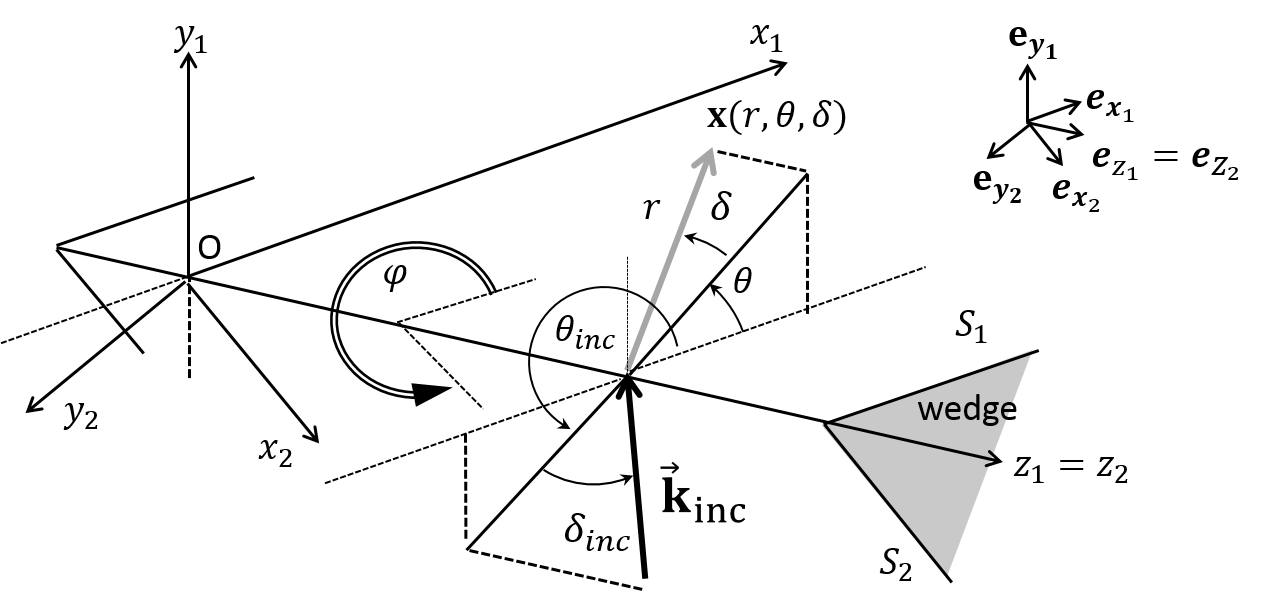
\includegraphics[width=\textwidth]{images/chapter4/wedge_3D.png}
\caption{Geometry of the problem}
\label{diedre_coords}
\end{figure}

Let us consider the problem of an elastic wave diffracted by a stress-free wedge delimited by faces $\mathcal{S}_1$ and $\mathcal{S}_2$. The geometry of the problem is shown on Fig.~\ref{diedre_coords}. The domain $\Omega$ is the inside of the wedge, defined by :
\begin{equation}
\Omega=\{ (r\cos \theta \cos \delta, r \sin \theta \cos \delta, r \sin \delta)\, \backslash \, \theta \in \rbrack 0, \varphi \lbrack, \, \delta \in \rbrack -\frac{\pi}{2}, \frac{\pi}{2} \lbrack \}
\end{equation}
%et sa surface
%$$ \mathcal{S}=\mathcal{S}_1 \cup \mathcal{S}_2 $$

The incident wave is a plane wave of the form
\begin{equation}
\mathbf{u}^{inc}(\mathbf{x},t)=\mathbf{A}_{\alpha}e^{i(\mathbf{k}_{\alpha}^{inc}\cdot \mathbf{x}-\omega t)}
\end{equation}
where $\mathbf{A}_{\alpha}$ is the amplitude vector of the incident wave and $\mathbf{k}_{\alpha}^{inc}$ is the incident wave vector. The type of the incident wave is denoted $\mathbf{k}_{\alpha}^{inc}$ (L for a longitudinal wave, TH for transverse horizontal and TV for transverse vertical). $(\mathbf{x}_1,\mathbf{y}_1, \mathbf{z}_1)$ is a Cartesian coordinate system associated to face $\mathcal{S}_1$. In this system, the incident wave vector is given by :
\begin{equation}
\mathbf{k}_{\alpha}^{inc}=\frac{\omega}{c_{\alpha}} \begin{pmatrix}
\cos\theta_{inc} \cos \delta_{inc} \\ \sin\theta_{inc} \cos \delta_{inc} \\
\sin \delta_{inc}
\end{pmatrix}
\end{equation}
As always, $c_L$ is the velocity of longitudinal waves and $c_T$ is the velocity of transverse waves.

The amplitude vector can be directed by three different and two-by-two orthogonal vectors, depending on the incident wave's polarization. These unit polarization vectors are noted $\hat{i}_*$, where $*=L, TH, TV$ and are given by Achenbach \cite{Achenbach} :
\begin{equation}
\hat{i}_L = \begin{pmatrix}
\cos\theta_{inc} \cos \delta_{inc} \\ \sin\theta_{inc} \cos \delta_{inc} \\
\pm \sin \delta_{inc}
\end{pmatrix}
\hfill
\hfill
\hat{i}_{TV} = \begin{pmatrix}
\mp\cos\theta_{inc} \sin \delta_{inc} \\ \mp\sin\theta_{inc} \sin \delta_{inc} \\
\cos \delta_{inc}
\end{pmatrix}
\hfill
\hfill
\hat{i}_{TH} = \begin{pmatrix}
-\sin\theta_{inc} \\ \cos\theta_{inc} \\
0
\end{pmatrix}
\label{C4:ivec}
\end{equation}
where the top sign gives the polarization of an incident wave and the bottom sign gives the polarization of a diffracted wave.

In all the following, vectors are expressed in the coordinate system $(\mathbf{x}_1,\mathbf{y}_1, \mathbf{z}_1)$, except when explicitly mentioned otherwise. For a homogeneous, isotropic material, the linear elasticity equation solved by the displacement field $\mathbf{u}$ is 
\begin{equation}
\underline{\mu} \Delta \mathbf{u} + (\underline{\lambda}+\underline{\mu})\nabla \nabla \mathbf{u} = \rho \frac{\partial^2 \mathbf{u}}{\partial t^2}
\label{C4:Elasticitelin}
\end{equation}
On each of the wedge faces, the displacement field verifies the zero-stress boundary conditions, expressed as :
\begin{equation}
(\underline{\lambda} \nabla \mathbf{u} .\mathbf{\mathbb{I}_3}+2\underline{\mu} \mathbf{\varepsilon} (\mathbf{u})).\mathbf{n}=0
\label{C4:stressfree}
\end{equation}
where $\mathbf{\mathbb{I}_3}$ is the identity matrix of the third order, $n$ is the inward facing normal to the wedge face ($n=\mathbf{y}_1$ on $\mathcal{S}_1$  and $n=\mathbf{y}_2$ on $\mathcal{S}_2$) and $\underline{\lambda}, \underline{\mu}$ are the Lamé coefficients of the considered elastic medium. The expression of the deformations tensor is :
\begin{equation}
\mathbf{\varepsilon}(\mathbf{u})=\frac{1}{2} \begin{pmatrix}
2\dfrac{\partial u_1}{\partial x_1} & \dfrac{\partial u_1}{\partial y_1}+\dfrac{\partial u_2}{\partial x_1}&\dfrac{\partial u_1}{\partial z}+\dfrac{\partial u_3}{\partial x_1} \\
\dfrac{\partial u_1}{\partial y_1}+\dfrac{\partial u_2}{\partial x_1}&2\dfrac{\partial u_2}{\partial y_1}&\dfrac{\partial u_2}{\partial z}+\dfrac{\partial u_3}{\partial y_1} \\
\dfrac{\partial u_1}{\partial z}+\dfrac{\partial u_3}{\partial x_1} &\dfrac{\partial u_2}{\partial z}+\dfrac{\partial u_3}{\partial y_1} & 2\dfrac{\partial u_3}{\partial z}
\end{pmatrix}
\end{equation}
Kamotski and Lebeau \cite{KamotskiLebeau} have proven existence and uniqueness of the solution to this problem in the 2D the case. We will suppose that their demonstration is still valid in the 3D case.

From hereon after, bold characters will be reserved to matrices in order to simplify notations. The solutions being time harmonic, the factor $e^{-i\omega t}$ will be implied but omitted everywhere. Furthermore, since there is no obstacle to propagation in the $z$ direction, $e^{i\frac{\omega}{c_{\alpha}}\sin\delta_{inc}z}$ is also a common factor to all the terms which appear in the solution.

The total field is written as the sum of an incident field $u^{inc}$ and a scattered field $u_0$
\begin{equation}
u=u_0+u^{inc}
\label{C4:scat}
\end{equation}

The dimensionless problem is obtained by applying the following variable change :
\begin{equation}
u_0(x,y,z)=v\left( \frac{\omega}{c_L} x, \frac{\omega}{c_L} y \right)e^{i\nu_{\beta}\sin\delta_{\beta}z}
\label{C4:adiming}
\end{equation}
where $\delta_{\beta}$ is the angle of Snell's cone of diffraction, the dimensionless Lamé parameters $\lambda,\mu$ are given by \eqref{LameAdim} and parameters $\nu_L$ and $\nu_T$ are defined by \eqref{nuLnuT}. Since $e^{i\nu_{\alpha}\sin\delta_{inc}z}$ is a common factor to all the terms of the solution, we can deduce Snell's law of diffraction :
\begin{equation}
\nu_{\alpha}\sin\delta_{inc}=\nu_{\beta}\sin\delta_{\beta}
\label{C4:Snelldiff}
\end{equation}
To simplify notations, we define the following parameter $\tau$ is defined by :
\begin{equation}
\tau=\nu_{\alpha}\sin\delta_{\alpha}
\label{deftau}
\end{equation}
Note that we therefore always have $\tau \in \lbrack -\nu_{\alpha}, \nu_{\alpha} \rbrack$. $u_0$'s $z$-dependency is entirely contained in the factor $e^{i\tau z}$ which will be implied but omitted in all the following.

Substituting \eqref{C4:scat} and \eqref{C4:adiming} into \eqref{C4:Elasticitelin} and \eqref{C4:stressfree} yields the dimensionless problem
\begin{eqnarray}
(\mathcal{P}^*) \hspace{2em} \left\{
\begin{array}{lr}
(E+1)v=0 & (\Omega) \\
Bv=-Bv_{\alpha}^{inc} & (\mathcal{S})
\end{array}
\right.
\label{C4:Padim}
\end{eqnarray}
where $(v_1,v_2,v_3)$ are the components of vector $v$ :
\begin{equation}
Ev=\mu (\Delta v -\tau^2 v)+(\lambda+\mu)
\begin{pmatrix}
\frac{\partial^2 v_1}{\partial x^2}+\frac{\partial^2 v_2}{\partial x \partial y} + i\tau\frac{\partial v_3}{\partial x} \\
\frac{\partial^2 v_1}{\partial x \partial y}+\frac{\partial^2 v_2}{\partial y^2}+ i\tau\frac{\partial v_3}{\partial y}\\
i\tau\left( \frac{\partial v_1}{\partial x}+\frac{\partial v_2}{\partial y}\right)-\tau^2 v_3
\end{pmatrix}
\label{C4:Eadim}
\end{equation}
and
\begin{equation}
Bv=\begin{pmatrix}
\mu \left(\frac{\partial v_x}{\partial y}+\frac{\partial v_y}{\partial x}\right) \\
\frac{\partial v_y}{\partial y}+\lambda\left( \frac{\partial v_x}{\partial x}+i\tau v_z\right)\\
\mu \left(\frac{\partial v_z}{\partial y}+i\tau v_y\right)
\end{pmatrix}
\label{C4:Badim}
\end{equation}
where $E$ and $B$ are respectively the dimensionless linear elasticity operator and normal stress operator. The first equation of system \eqref{C4:Padim} is the dimensionless version of the linear elasticity equation and the second equation is the dimensionless version of the stress-free boundary conditions.

\section{Integral formulation of the solution}
As for the previous cases, the first step in solving problem $(\mathcal{P}^{\alpha})$ is to formulate the solution as an integral. 
\subsection{Limiting absorption principle}
The limiting absorption principle is applied to $(\mathcal{P}^{\alpha})$. This means that it is considered as a special case $(\varepsilon=0)$ of the problem
\begin{eqnarray}
(\mathcal{P}^*_{\epsilon}) \hspace{2em} \left\{
\begin{array}{lr}
(E+e^{-2i\epsilon})v^{\epsilon}=0 & (\Omega) \\
Bv^{\epsilon}=-Bv_*^{inc} & (\mathcal{S})
\end{array}
\right.
\label{C4:Pabs}
\end{eqnarray}
Following Kamotski and Lebeau \cite{KamotskiLebeau}, we will once again suppose that the solution can be expressed as the sum of two contributions, corresponding to each of the wedge faces :
\begin{equation}
v^{\epsilon}=v_1^{\epsilon}+v_2^{\epsilon}
\label{C4:v1+v2}
\end{equation}
where functions $v_j^{\epsilon}$ are now defined on all of  $\mathbb{R}^3$ by
\begin{equation}
v_j^{\epsilon}=-(E+e^{-2i\epsilon})^{-1} \begin{bmatrix}
\begin{pmatrix}
\alpha_j \\
\beta_j \\
\gamma_j
\end{pmatrix}
\otimes \delta_{\mathcal{S}_j}
\end{bmatrix}
\label{C4:vjdef}
\end{equation}
Distributions $\alpha_j,\beta_j, \gamma_j $ are unknown and are supposed to belong to the special call $\mathcal{A}$ defined in \ref{defClassA}. We can now define the outgoing solution of $(\mathcal{P}^{\alpha})$ analogously to the 2D case :
\begin{definition}
	 v is called an outgoing solution of equation \eqref{C4:Padim} if v is a solution of the form
	\begin{equation}
	\label{C4:decomposition}
	v=v_1|_{\Omega}+v_2|_{\Omega}
	\end{equation}
	where, for $j=1,2$ :
	\begin{equation}
	\label{C4:inv_potentiels}
	v_j=-\lim_{\epsilon \to 0} (E+e^{-2i\epsilon})^{-1} \begin{bmatrix}
\begin{pmatrix}
\alpha_j \\
\beta_j \\
\gamma_j
\end{pmatrix}
\otimes \delta_{\mathcal{S}_j}
\end{bmatrix}
	\end{equation}
	where $\alpha_j,\beta_j,\gamma_j \in \mathcal{A}$. %and where $\delta_{\mathcal{S}_1}$ and $\delta_{\mathcal{S}_2}$ sont les distributions de Dirac associés aux faces $\mathcal{S}_1$ et $\mathcal{S}_2$ du dièdre respectivement.
\end{definition}
The following theorem was proved by Kamotski and Lebeau \cite{KamotskiLebeau} in the 2D case. We will suppose that their proof can be adapted to the 3D case and that the theorem is still true.
\begin{theorem}
Equation \eqref{C4:Padim} admits a unique outgoing solution.
\end{theorem}
Nous that the outgoing solution has been defined, we will derive an integral formulation of this solution.

\subsection{Integral formulation}
The two-sided Fourier transform and its inverse transform are defined by \eqref{fullfourierdef}. The first step in determining an integral formulation of the solution is to apply the two-sided Fourier transform to \eqref{C4:vjdef}. This possible because all the distributions that appear in this equation are tempered distributions and they therefore admit a Fourier transform. We then have :
\begin{equation}
\hat{v}^{\epsilon}_j(\xi,\eta)=(\mathbf{M}-e^{-2i\epsilon}\mathbf{\mathbb{I}_3})^{-1}\Sigma_j(\xi)
\label{C4:matMvjeps}
\end{equation}
where $\Sigma_j, j=1,2$  are the unknown spectral functions, defined by :
\begin{equation}
\Sigma_j(\xi,)=\begin{pmatrix}
\hat{\alpha_j}(\xi)\\ \hat{\beta_j}(\xi) \\ \hat{\gamma_j}(\xi)
\end{pmatrix}
\end{equation}
and where \textbf{M} is the two-sided Fourier transform of operator $E$. Its expression is :
\begin{equation}
\mathbf{M}(\xi,\eta)=
\begin{pmatrix}
\xi^2+\mu(\eta^2+\tau^2) & (\lambda+\mu)\xi \eta & (\lambda+\mu)\xi\tau \\
 (\lambda+\mu)\xi \eta & \eta^2+\mu(\xi^2+\tau^2) & (\lambda+\mu)\eta\tau \\
(\lambda+\mu)\xi\tau & (\lambda+\mu)\eta\tau & \tau^2+\mu(\xi^2+\eta^2) 
\end{pmatrix}
\label{C4:matM}
\end{equation}
Substituting $\lambda$ by $1-2\mu$ and $\mu$ by $1/\nu_T^2$, \eqref{C4:matM} yields
\begin{multline}
(\mathbf{M}-e^{-2i\epsilon}\mathbb{I}_3)^{-1}=\\
\frac{\begin{pmatrix}
\xi^2+\nu_T^2(\eta^2+\tau^2-e^{-2i\epsilon}) & (1-\nu_T^2)\xi \eta & (1-\nu_T^2)\xi \tau \\
(1-\nu_T^2)\xi \eta & \eta^2+\nu_T^2(\xi^2+\tau^2-e^{-2i\epsilon}) & (1-\nu_T^2)\tau \eta \\
(1-\nu_T^2)\xi \tau & (1-\nu_T^2)\tau \eta & \tau^2+\nu_T^2(\eta^2+\xi^2-e^{-2i\epsilon})
\end{pmatrix}}{(\xi^2+\eta^2+\tau^2-e^{-2i\epsilon})(\xi^2+\eta^2+\tau^2-\nu_T^2e^{-2i\epsilon})} 
\end{multline}

Finally, the integral formulation of $v_j$ is obtained by inverting the two-sided Fourier transform applied in \eqref{C4:matMvjeps} :
\begin{equation}
v_j^{\epsilon}(x_j,y_j)=\frac{1}{4\pi^2}\int_{\mathbb{R}^2} e^{i x_j\xi}\left( \int_{-\infty}^{+\infty}e^{iy_j\eta} (\mathbf{M}-e^{-2i\epsilon}\mathbf{\mathbb{I}_3})^{-1} \,d\eta \right) \Sigma_j(\xi) \,d\xi
 \label{C4:invdouble}
\end{equation}

The poles of $(\mathbf{M}-e^{-2i\epsilon}\mathbf{\mathbb{I}_3})^{-1}$ are located in $\eta=\pm \zeta_*^{\epsilon}(\xi)$, where $*=L,T$ and
\begin{equation}
\zeta_*^{\epsilon}(\xi)=\sqrt{e^{-2i\epsilon}\nu^2_*-(\xi^2+\tau^2)}
\end{equation}
Let us define $\nuti_*, *=L,T$ by
\begin{equation}
\nuti_*^{\epsilon}=\sqrt{e^{-2i\epsilon}\nu_*^2-\tau^2}
\label{defnutieps}
\end{equation}
If the incident wave is longitudinal, then $\nuti \in \mathbb{R}$. However, if the incident wave is transverse, then two cases may occur :
\begin{itemize}
	\item if $|\sin\delta_{inc}| \leq \frac{\nu_L}{\nu_T}$, then $\nuti_L \in \mathbb{R}$
	\item if $|\sin\delta_{inc}| >\frac{\nu_L}{\nu_T}$, then $\nuti_L=i\eta_L \in i\mathbb{R}$ 
\end{itemize} 
In any case,
\begin{equation}
\zeta_*^{\epsilon}(\xi)=\sqrt{\tilde{\nu}_*^{\epsilon^2}-\xi^2}
\end{equation}
The chosen branch cut is the one for which the square root's imaginary part is positive. It is defined by
 \begin{eqnarray}
 \zeta_*(\xi)=
 \left\{
 \begin{array}{lr}
 i\sqrt{\xi^2-\tilde{\nu}_*^2}& \mbox{si } |\xi| \geq |\nuti_*| \\
 -\sqrt{\tilde{\nu}_*^2-\xi^2}& \mbox{si } |\xi| \leq |\nuti_*|
 \end{array}
 \right.
 \label{defzeta}
 \end{eqnarray}
%La racine carrée complexe étant définie au signe près, $\sqrt{z}$ peut prendre deux valeurs distinctes pour $z$ fixé. C'est ce qu'on appelle les branches de coupure de la fonction. Les points de branchement sont les valeurs pour lesquelles ces branches se croisent (ici il s'agit de $\xi=\pm \tilde{\nu}_*^{\epsilon}$). Afin de bien définir $\zeta_*^{\epsilon}(\xi)$, on choisit la branche dont la partie imaginaire est positive. 

The inner integral of \eqref{C4:invdouble} is computed using Cauchy's residue theorem :
\begin{equation}
v_j^{\epsilon}(x_j,y_j)=\frac{i}{4\pi}e^{2i\epsilon}\int_{\mathbb{R}} e^{ix_j\xi}\sum_{*=L,T}e^{i|y_j|\zeta_*^{\epsilon}(\xi)}\mathbf{M_*}(\xi,\mbox{sgn }y_j)\Sigma_j(\xi)\,d\xi
\label{C4:vjeps}
\end{equation}
where $\mathbf{M_*}(\xi,t),$ and $t=\mbox{sgn}( y_j)$ are defined by
\begin{subequations}
\begin{equation}
\mathbf{M_L}(\xi,t)=\begin{pmatrix}
\frac{\xi^2}{\zeta_L^{\epsilon}} &t\xi & \frac{\xi\tau}{\zeta_L^{\epsilon}} \\
t\xi & \zeta_L^{\epsilon} & t\tau \\
\frac{\xi\tau}{\zeta_L^{\epsilon}}& t\tau & \frac{\tau^2}{\zeta_L^{\epsilon}}
\end{pmatrix}
\label{C4:MLeps}
\end{equation}
\begin{equation}
\mathbf{M_T^{\epsilon}}(\xi,t)=\begin{pmatrix}
\zeta_T^{\epsilon} +\frac{\tau^2}{\zeta_T^{\epsilon}}& -t\xi &-\frac{\xi\tau}{\zeta_T^{\epsilon}}\\
-t\xi & \frac{\xi^2+\tau^2}{\zeta_T^{\epsilon}}&-t\tau \\
-\frac{\xi\tau}{\zeta_T^{\epsilon}}&-t\tau&\zeta_T^{\epsilon} +\frac{\xi^2}{\zeta_T^{\epsilon}}
\end{pmatrix}
\label{C4:MTeps}
\end{equation}
\label{C4:M*eps}
\end{subequations}

These matrices can be computed in two different manners, providing a way to test this result. the first way to compute these matrices is by direct computation of the residues of matrix $(\mathbf{M}-e^{-2i\epsilon}\mathbf{\mathbb{I}_3})^{-1}$. The second option for computing these matrices is by computing the eigen vectors and eigen values of $\mathbf{M}$. %On trouve bien les mêmes résultats avec les deux méthodes.

The three eigen vectors of $\mathbf{M}$ and the corresponding eigen values are :
\begin{subequations}
\begin{equation}
    \mathbf{M}\begin{pmatrix}
    \xi \\ \eta \\ \tau 
    \end{pmatrix}
    =(\xi^2+\eta^2+\tau^2)\begin{pmatrix}
    \xi \\ \eta \\ \tau 
    \end{pmatrix}
\end{equation}
\begin{equation}
   \mathbf{M}\begin{pmatrix}
    -\eta \\ \xi \\ 0
    \end{pmatrix}
    =\frac{\xi^2+\eta^2+\tau^2}{\nu_T^2}\begin{pmatrix}
    \xi \\ \eta \\ \tau 
    \end{pmatrix} 
\end{equation}
\begin{equation}
   \mathbf{M}\begin{pmatrix}
    -\xi\tau \\ \eta\tau \\ \xi^2+\eta^2
    \end{pmatrix}
    =\frac{\xi^2+\eta^2+\tau^2}{\nu_T^2}\begin{pmatrix}
    -\xi\tau \\ \eta\tau \\ \xi^2+\eta^2
    \end{pmatrix} 
\end{equation}
\end{subequations}
These three vectors are linearly independent and constitute a vector basis of $\mathbb{C}^3$. This means that any vector of $\mathbb{C}^3$ can be expressed as a linear combination of these three vectors. Notably :
\begin{equation}
    \begin{pmatrix}
    \hat{\alpha}_j\\ \hat{\beta}_j\\ \hat{\gamma}_j
    \end{pmatrix}
    = \frac{\xi\hat{\alpha}_j+\eta\hat{\beta}_j+\tau\hat{\gamma}_j}{\xi^2+\eta^2+\tau^2}\begin{pmatrix}
    \xi \\ \eta \\ \tau 
    \end{pmatrix} + \frac{\xi\hat{\beta}_j-\eta\hat{\alpha}_j}{\xi^2+\eta^2} \begin{pmatrix}
    -\eta \\ \xi \\ 0
    \end{pmatrix} + \frac{(\xi^2+\eta^2)\hat{\gamma}_j-\tau(\xi\hat{\alpha}_j+\eta\hat{\beta}_j)}{(\xi^2+\eta^2)(\xi^2+\eta^2+\tau^2)} \begin{pmatrix}
    -\xi\tau \\ \eta\tau \\ \xi^2+\eta^2
    \end{pmatrix}
\end{equation}
This second computation method thus yields
\begin{equation}
v_j^{\epsilon}(x_j,y_j)=\frac{i}{4\pi}e^{2i\epsilon}\int_{\mathbb{R}} e^{ix_j\xi}\sum_{*=L,TH,TV}e^{i|y_j|\zeta_*^{\epsilon}(\xi)}\mathbf{M_*}(\xi,\mbox{sgn }y_j)\Sigma_j(\xi)\,d\xi
\label{C4:vjeps2}
\end{equation}
where $\mathbf{M_L}(\xi,t),$ is given by \eqref{C4:MLeps} and
\begin{subequations}
\begin{equation}
\mathbf{M_{TV}}(\xi,t)=\begin{pmatrix}
\frac{\xi^2\tau^2}{\zeta_T(\xi^2+\zeta^2)}&\frac{t\xi\tau^2}{\xi^2+\zeta_T^2}&\frac{-\xi\tau}{\zeta_T}\\
\frac{t\xi\tau^2}{\xi^2+\zeta_T^2}&\frac{\zeta_T\tau^2}{\xi^2+\zeta_T^2}&-t\tau\\
\frac{-\xi\tau}{\zeta_T}&-t\tau&\frac{\xi^2+\zeta_T^2}{\zeta_T}
\end{pmatrix}
\label{C4:MTVeps}
\end{equation}
\begin{equation}
\mathbf{M_{TH}}(\xi,t)=\left(1+\frac{\tau^2}{\xi^2+\zeta_T^2}\right)\begin{pmatrix}
\zeta_T&-t\xi&0\\
-t\xi&\frac{\xi^2}{\zeta_T}&0\\
0&0&0
\end{pmatrix}
\label{C4:MTHeps}
\end{equation}
\label{C4:M*eps2}
\end{subequations}
Note that $ \mathbf{M_T}=\mathbf{M_{TH}}+\mathbf{M_{TV}}$. Expressions \eqref{C4:vjeps} and \eqref{C4:vjeps2} are equivalent.

Integral \eqref{C4:vjeps} is well defined for all values of $\epsilon \in \rbrack 0, \pi \lbrack $, since for these values of $\epsilon$, the integration contour never crosses the branch points of the integrand, which are located at $\xi=\pm \tilde{\nu}_*^{\epsilon}$, outside of the real axis.

According to Croisille et Lebeau \cite{CroisilleLebeau}, convergence in the 2D case is verified for $\epsilon \rightarrow 0$. We will suppose that this is still the case in 3D. The deformation contour $\mathbb{R}$ is deformed into contour $\Gamma_{0}$, visible on Fig.~\ref{C4:Gamma0_noncr} in the case where $\nuti_L\in\mathbb{R}$ and on Fig.~\ref{C4:Gamma0_cr} in the other case. This way the branch points of the integrand are avoided.

In all the following, superscript $\epsilon=0$ will be omitted in order to alleviate notations. Finally:
\begin{equation}
v_j(x_j,y_j)=\frac{i}{4\pi}\int_{\Gamma_0} e^{ix_j\xi}\sum_{*=L,T}e^{i|y_j|\zeta_*(\xi)}\mathbf{M_*}(\xi,\mbox{sgn }y_j)\Sigma_j(\xi)\,d\xi
\label{C4:vj0}
\end{equation}

\begin{figure}
\centering
\begin{subfigure}[b]{0.45\textwidth}
\begin{tikzpicture}
\node at (0,0) {$\times$};
\node at (0.35,0.35) {$0$};
\node at (2.25,0) {$\times$}; % Pole
\node at (1.5,0) {$\times$}; %pole
\node at (1.5,-0.45) {$\tilde{\nu}_L$};
\node at (2.25,-0.45) {$\tilde{\nu}_T$};
\node at (-1.5,0) {$\times$};
\node at (-2.25,0) {$\times$};
\node at (-1.5,0.45) {$-\tilde{\nu}_L$}; %pole
\node at (-2.25,0.45) {$-\tilde{\nu}_T$}; %pole
\node at (3.25,0.38) {$(\Gamma_0)$};
\node at (3.7,-0.38) {$\xi_1$};
\node at (0.38,2.25) {$\xi_2$};
%\draw[ thick, ->] (-2.5,-0.5) arc (180:235:1);
%\node at (-2.7,-0.9) {$F_1$};
%\draw[ thick, ->] (2.5,0.5) arc (0:45:1); %ici c'est les fleches 
%\node at (2.7,0.9) {$F_2$};
\draw[thick,black,yshift=0pt,decoration={markings,
mark=at position 1 with {\arrow{stealth}}},
postaction={decorate}](0,-2.5) -- (0,2.5);
\draw[thick,black,yshift=0pt,
decoration={ markings,  % This schema allows for fine-tuning the positions of arrows 
      mark=at position 0.1 with {\arrow{latex}},
      mark=at position 0.6 with {\arrow{latex}},
      mark=at position 0.9 with {\arrow{latex}},
      mark=at position 1 with {\arrow{stealth}}},
      postaction={decorate}]
      (-4,0) -- (-2.5,0)  arc (-180:0:0.25) -- (-1.75,0)  arc (-180:0:0.25)  -- (1.25,0)arc (180:0:0.25)  -- (2,0)arc (180:0:0.25) -- (3.75,0); % ca c'est l'axe
\end{tikzpicture}
\caption{Contour $\Gamma_0$ in the case where $\nuti_L \in \mathbb{R}$}
\label{C4:Gamma0_noncr}
\end{subfigure}
\hfill
\centering
\begin{subfigure}[b]{0.45\textwidth}
\begin{tikzpicture}
\node at (0,0) {$\times$};
\node at (0.35,0.35) {$0$};
\node at (2.25,0) {$\times$}; %pole
\node at (2.25,-0.45) {$\tilde{\nu}_T$};
\node at (-2.25,0) {$\times$};
\node at (-2.25,0.45) {$-\tilde{\nu}_T$}; %pole
\node at (3.5,0.38) {$(\Gamma_0)$};
\node at (0,1.5) {$\times$};
\node at (0.45, 1.5) {$\nuti_L$};
\node at (0,-1.5) {$\times$};
\node at (0.45,-1.5) {$-\nuti_L$};
\node at (3.9,-0.38) {$\xi_1$};
\node at (0.38,2.25) {$\xi_2$};
\draw[thick,black,yshift=0pt,decoration={markings,
mark=at position 0.99 with {\arrow{stealth}}},
postaction={decorate}](0,-2.5) -- (0,2.5);
\draw[thick,black,yshift=0pt,
decoration={ markings,  % This schema allows for fine-tuning the positions of arrows 
      mark=at position 0.1 with {\arrow{latex}},
      mark=at position 0.6 with {\arrow{latex}},
      mark=at position 0.9 with {\arrow{latex}},
      mark=at position 0.99 with {\arrow{stealth}}},
     postaction={decorate}]
      (-3.75,0) -- (-2.5,0)  arc (-180:0:0.25) -- (2,0)arc (180:0:0.25) -- (4,0); % ca c'est l'axe
\end{tikzpicture}
\caption{Contour $\Gamma_0$ in the case where $\nuti_L \in i\mathbb{R}$}
\label{C4:Gamma0_cr}
\end{subfigure}
\caption{Contour $\Gamma_0$ in the complex plane $\xi=\xi_1+i\xi_2$}
\label{C4:Gamma0}
\end{figure}


\subsection{Far field approximation}
$x=(x_1,y_1,z_1)=(r\cos\theta\cos\delta_{\beta},r\sin\theta\cos\delta_{\beta},r\sin\delta_{\beta})$ is an observation point, indexed by its spherical coordinates, visible on Fig.~\ref{diedre_coords}. In order for the diffracted field to be observable at this point, $x$ is located on one of Keller's cones of diffraction, visible on Fig.~\ref{C4:Kellercone}. The observation skew angle $\delta_{\beta}$ is set by Snell's law of diffraction \eqref{C4:Snelldiff}.

\begin{figure}
\centering
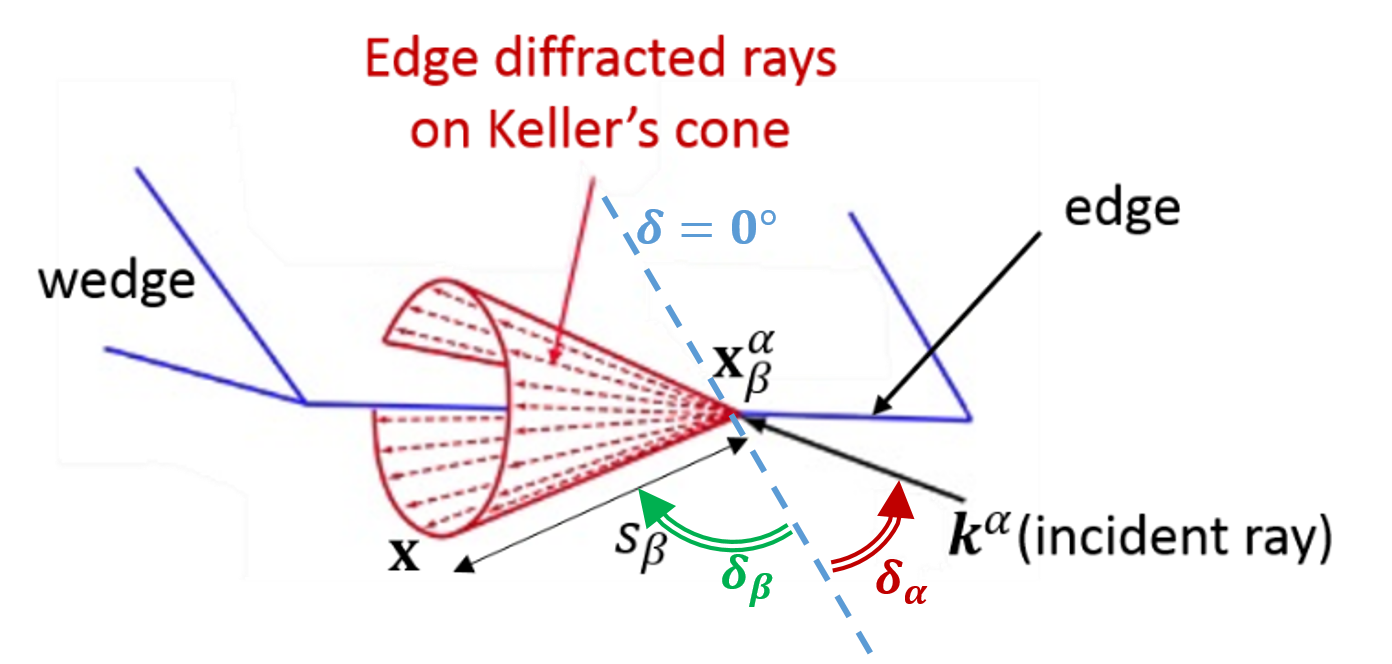
\includegraphics[width=\textwidth]{images/chapter4/Keller_annotated.png}
        \caption{Keller's cone of diffraction}
        \label{C4:Kellercone}
\end{figure}

According to \eqref{C4:adiming},the scattered field at point $P$ is :
\begin{equation}
u_0(x_1,y_1,z)=v(\frac{\omega}{c_L}r\cos\theta\cos\delta_{\beta},\frac{\omega}{c_L}r\sin\theta\cos\delta_{\beta})e^{ik_{\beta}\sin\delta_{\beta}z}
\end{equation}
The far field parameter is $R=\frac{\omega r}{c_L}$. The aim is to determine the asymptotic behavior of $v(R\cos\theta\cos\delta_{\beta},R\sin\theta\cos\delta_{\beta})$ when $R\rightarrow +\infty$.The first step is to apply the change following of variables in integral $v_1$ :
\begin{equation}
\begin{split}
\xi&=\tilde{\nu}_*\cos\lambda \\
d\xi&=-\tilde{\nu}_*\sin\lambda\, d\lambda
\end{split}
\label{C4:changevar2}
\end{equation}
yielding
\begin{equation}
v_1(r,\theta,\delta_{\beta})=\frac{i}{4\pi} \int_{C_0}\sum_{*=L,T}\tilde{\nu}_*^2 e^{i\tilde{\nu}_*R\cos\delta_{\beta}\cos(\lambda+\bar{\theta})}\mathbf{ P_*}(\lambda,t)\Sigma_1(\tilde{\nu}_*\cos\lambda) \, d \lambda
\label{C4:v1C0}
\end{equation}
where $\bar{\theta}$ has been defined by \eqref{obs} and
\begin{equation}
\mathbf{P_L}(\lambda,t)=
\begin{pmatrix}
\cos^2\lambda & -t\cos\lambda\sin\lambda &\frac{\tau}{\tilde{\nu}_L} \cos\lambda \\
-t\cos\lambda\sin\lambda & \sin^2\lambda&-t\frac{\tau}{\tilde{\nu}_L}\sin\lambda \\
\frac{\tau}{\tilde{\nu}_L} \cos\lambda&-t\frac{\tau}{\tilde{\nu}_L}\sin\lambda&\frac{\tau^2}{\tilde{\nu}_L^2}
\end{pmatrix}
\end{equation}
and
\begin{equation}
\mathbf{P_T}(\lambda,t)=
\begin{pmatrix}
\sin^2\lambda+\frac{\tau^2}{\tilde{\nu}_T^2} & t\cos\lambda\sin\lambda &-\frac{\tau}{\tilde{\nu}_T}\cos\lambda \\
t\cos\lambda\sin\lambda & \cos^2\lambda+\frac{\tau^2}{\tilde{\nu}_T^2}&t\frac{\tau}{\tilde{\nu}_T}\sin\lambda \\
-\frac{\tau}{\tilde{\nu}_T}\cos\lambda&t\frac{\tau}{\tilde{\nu}_T}\sin\lambda&1
\end{pmatrix}
\end{equation}
$t=\mbox{sgn} \sin\theta$ and contour $C_0$ is visible on Fig.~\ref{C4:steepestcontour}.

Note that in the case $\nuti_L =i\eta_L \in i\mathbb{R}$, variable change \eqref{C4:changevar2} produces an evanescent term :
\begin{equation}
\begin{split}
v_1(r,\theta,\delta_{\beta})&=-\frac{i}{4\pi} \int_{C_0^L}\eta_L^2 e^{-\eta_L R\cos\delta\cos(\lambda+\bar{\theta})}\mathbf{ P_L}(\lambda,t)\Sigma_1(i\eta_L\cos\lambda) \, d\lambda\\
&+\frac{i}{4\pi} \int_{C_0}\tilde{\nu}_T^2 e^{i\nuti_T R\cos\delta\cos(\lambda+\bar{\theta)})}\mathbf{ P_T}(\lambda,t)\Sigma_1(\tilde{\nu}_T\cos\lambda) \, d\lambda
\end{split}
\label{C4:v1C0evan}
\end{equation}
where contour $C_0^L$ is visible on Fig.~\ref{C4:steepestcontour}. The exponential term in the first integral of \eqref{C4:v1C0evan} is $e^{-\eta_L R\cos\delta\cos(\lambda+\bar{\theta})}$, where $\eta_L>0$, $R>0$ and $\cos\delta>0$. Furthermore, for $\lambda :\in C_0^L$, we have :
\begin{equation}
\lambda=-\left(\dfrac{\pi}{2}^+\right)+i\lambda_2
\end{equation}
where the notation $\dfrac{\pi}{2}^+$ refers to a real number which tends to $\frac{\pi}{2}$ with superior values and $\lambda_2=\rm Im(\lambda)$. This yields
\begin{equation}
\cos(\lambda+\bar{\theta})=\cos(\bar{\theta}-\dfrac{\pi}{2})\cosh\lambda_2-i\sin(\bar{\theta}-\dfrac{\pi}{2})\sinh\lambda_2
\end{equation}
Having $\bar{\theta} \in \lbrack 0,\pi \rbrack$, we have $\cos(\bar{\theta}-\dfrac{\pi}{2})=\sin\bar{\theta}\leq 0$ and 
\begin{equation}
|e^{-\eta_L R\cos\delta\cos(\lambda+\bar{\theta})}|=e^{-\eta_L R\cos\delta\sin\bar{\theta}\cosh\lambda_2}
\end{equation}
The amplitude of the integrand in the first integral of \eqref{C4:v1C0evan} decreases exponentially as the distance from the edge grows. %This means that it is an evanescent term.

\begin{figure}
\centering
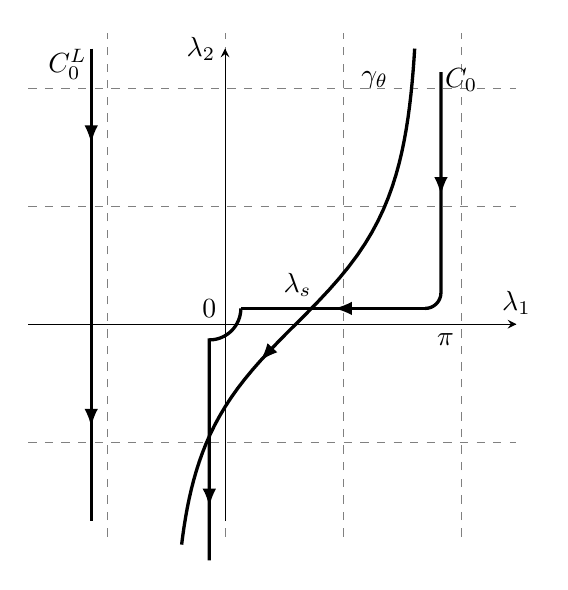
\begin{tikzpicture}
	\draw[step=1.5cm,gray,very thin,dashed](-2.5,-2.7)grid(3.7,3.7);
	\draw[thin, decoration={ markings,  
		mark=at position 1 with {\arrow{stealth}}},
	postaction={decorate}] (-2.5,0)  -- (3.7,0) node[above]{$\lambda_1$};
	\draw[thin, decoration={ markings,  
		mark=at position 1 with {\arrow{stealth}}},
	postaction={decorate}](0,-2.5)--(0,3.5) node[left]{$\lambda_2$};

	\node at (2.8,-0.2) {$\pi$};
	\node at (-0.2,0.2) {$0$};
	\node at (0.92,0.5) {$\lambda_s$};
	\node at (3,3.1) {$C_0$};
	\node at (1.9,3.1) {$\gamma_{\theta}$};
	\node at (-2.0,3.3) {$C_0^L$};
	
	\draw[black,very thick, decoration={ markings,  
		mark=at position 0.2 with {\arrow{latex}},
		mark=at position 0.8 with {\arrow{latex}}},
	postaction={decorate}] (-1.7,3.5)--(-1.7,-2.5);
	
	\draw[black,very thick][domain=0:3.5] plot({2*pi/7 + acos(1/cosh(\x))*pi/180},\x);
	\draw[black,very thick, decoration={ markings,  
		mark=at position 0.2 with {\arrow{latex}}},
	postaction={decorate}][domain=0:-2.8] plot({2*pi/7 - acos(1/cosh(\x))*pi/180},\x);
	
	\draw[very thick,black,%xshift=0pt,
	decoration={ markings,  
		mark=at position 0.8 with {\arrow{latex}}},
	postaction={decorate}]
	(0.2,0.2) arc (0:-90:0.4) -- (-0.2,-3); 
	
	\draw[very thick,black,%yshift=0pt,
	decoration={ markings, mark=at position 0.5 with {\arrow{latex}}}, postaction={decorate}]
	(pi-0.57,0.2) -- (0.2,0.2);

	\draw[very thick,black,%xshift=0pt,
	decoration={ markings,  
		mark=at position 0.5 with {\arrow{latex}}},
	postaction={decorate}]
	(pi-0.4,3.2) -- (pi-0.4,0.4) arc (0:-90:0.2) ;

	\end{tikzpicture}
	\caption{Contours $C_0$ and $\gamma_{\theta}$ in the complex plane $\lambda=\lambda_1+i\lambda_2$. The stationary phase points are noted $\lambda_s$.}
	\label{C4:steepestcontour}
\end{figure}

The far-field evaluation of the integral is obtained by applying the steepest descent method, presented in appendix \ref{PhaseStationnaire}, to \eqref{C4:v1C0}. To do so, contour $C_0$ is deformed into contour $\gamma_{\theta}$, also visible in Fig.~\ref{C4:steepestcontour}. In the case $\nuti_L \in \mathbb{R}$, this leads to
\begin{equation}
v_1=v_1^{sing}+v_1^{diff}
\end{equation}
where $v_1^{sing}$ is the contribution of all the singularities of the spectral functions crossed during the deformation from $C_0$ to $\gamma_{\theta}$, corresponding to the reflected and head waves, and $v_1^{diff}$ is the contribution of the stationary phase point, corresponding to the diffracted wave and computed using \eqref{steepformula}. Only the contribution of the diffracted waves will be computed here. In order to simplify notations, we will note $\mathbf{P}_*(\lambda,1)=\mathbf{P}_*(\lambda)$ and $\mathbf{P}_*(\lambda,-1)=\mathbf{P}_*(-\lambda)$). The contribution of diffracted waves is 
\begin{equation}
v_1^{diff}(r,\theta,\delta_{\beta})=\frac{e^{-i\pi/4}}{2\sqrt{2\pi}}\sum_{*=L,T}\tilde{\nu}_*^2\frac{e^{-i\tilde{\nu}_*R\cos\delta_{\beta}}}{\sqrt{\nuti_*R\cos\delta_{\beta}}}\mathbf{P_*}(\pi-\theta)\Sigma_1(-\tilde{\nu}_*\cos\theta)
\end{equation}
Analogously,
\begin{equation}
v_2^{diff}(r,\varphi-\theta,\delta_{\beta})=\frac{e^{-i\pi/4}}{2\sqrt{2\pi}}\sum_{*=L,T}\tilde{\nu}_*^2\frac{e^{-i\tilde{\nu}_*R\cos\delta_{\beta}}}{\sqrt{\nuti_*R\cos\delta_{\beta}}}\mathbf{P_*}(\pi-(\varphi-\theta))\Sigma_1(-\tilde{\nu}_*\cos(\varphi-\theta))
\end{equation}

In the case where $\nuti_L=i\eta_L \in i\mathbb{R}$, the far-field evaluation is obtained by applying the steepest descent method, presented in appendix \ref{PhaseStationnaire}, to \eqref{C4:v1C0evan}. Contour $C_0$ is deformed into contour $\gamma_{\theta}$ and contour $C_0^L$ is deformed into contour $\gamma_{\theta}^L$. This leads to
\begin{equation}
v_1=v_1^{sing}+v_1^{diff}+v_1^{evan}
\end{equation}
where $v_1^{sing}$ is the contribution of all the singularities of the spectral functions crossed during the deformation from $C_0$ to $\gamma_{\theta}$, $v_1^{diff}$ is the contribution of the stationary phase point to the integral on $C_0$, corresponding to the diffracted wave, and $v_1^{evan}$ is the contribution of the integral on $C_0^L$, which decays exponentially as the far-field parameter $R$ grows, making it an evanescent wave. Once again, only the contribution of the diffracted waves will be computed here. Contribution $v_1^{diff}$ is computed using \eqref{steepformula} :
%. The contribution of evanescent waves is 
%\begin{equation}
%v^{evan}_1(R\cos\theta,R\sin\theta)= \sqrt{\frac{2\pi}{R\eta_L\cos\delta_{\beta}}} e^{-R\eta_L\cos\delta}\mathbf{P_L}(-\theta)\Sigma_1(i\eta_L\cos\theta)
%\end{equation}
%and the contribution of diffracted waves is :
\begin{equation}
v_1^{diff}(r,\theta,\delta_{\beta})=\frac{e^{-i\pi/4}}{2\sqrt{2\pi}}\tilde{\nu}_T^2\frac{e^{-i\tilde{\nu}_TR\cos\delta_{\beta}}}{\sqrt{\nuti_TR\cos\delta_{\beta}}}\mathbf{P_T}(\pi-\theta)\Sigma_1(-\tilde{\nu}_T\cos\theta)
\end{equation}
Analogously,
%\begin{equation}
%v^{evan}_2(R\cos\theta,R\sin\theta)= \sqrt{\frac{2\pi}{R\eta_L\cos\delta_{\beta}}} e^{-R\eta_L\cos\delta}\mathbf{P_L}(-(\varphi-\theta))\Sigma_1(i\eta_L\cos(\varphi-\theta))
%\end{equation}
%and
\begin{equation}
v_2^{diff}(r,\varphi-\theta,\delta_{\beta})=\frac{e^{-i\pi/4}}{2\sqrt{2\pi}}\tilde{\nu}_T^2\frac{e^{-i\tilde{\nu}_TR\cos\delta_{\beta}}}{\sqrt{\nuti_TR\cos\delta_{\beta}}}\mathbf{P_T}(\pi-(\varphi-\theta))\Sigma_2(-\tilde{\nu}_T\cos(\varphi-\theta))
\end{equation}
In any case, the total diffracted field is
\begin{equation}
v^{diff}=v_1^{diff}+v_2^{diff}
\end{equation}

Let us now isolate L, TH and TV diffracted waves in order to compute the corresponding diffraction coefficients, defined by
\begin{equation}
v_{\beta}^{diff}(r,\theta,\delta_{\beta})=D_{\beta}^{\alpha}(\theta)\frac{e^{-i\nuti_{\beta}R\cos\delta_{\beta}}}{\sqrt{\nuti_{\beta}R\cos\delta_{\beta}}} v^{inc}(R\cos\theta,R\sin\theta) \hat{i}_{\beta}
\label{C4:coeffdiff}
\end{equation}
Using the expressions of the unit vectors given by \eqref{ivec}, the $\beta$ diffracted wave is given by $v^{diff}\cdot \hat{i}_{\beta}$. This yields :
\begin{equation}
D_{\beta}^{\alpha}(\theta)=\frac{e^{-i\pi/4}}{2\sqrt{2\pi}}\sum_{j=1,2}\nuti_{\beta}^2 \,{}^t \Sigma_j(-\nuti_{\beta}\cos\theta_j)\cdot\left(\mathbf{P}_{\beta}(\pi-\theta_j).\hat{i}_{\beta}\right)
\label{C4:Dbeta}
\end{equation}
where $\theta_1=\theta$ and $\theta_2=\varphi-\theta$.

In order to determine the field diffracted by a wedge illuminated by an incident plane wave, it is sufficient to compute the diffraction coefficient. This coefficient has been expressed in terms of two unknown functions called the spectral functions. The semi-analytical computation of these functions is presented in the following section

\section{Semi-analytical evaluation of the spectral functions}
The first step in computing the spectral functions is to determine a system of functional equations of which they are a solution. We will then show that these functions can be decomposed into two parts : a singular function, computed analytically, and a regular function, approached numerically.
\subsection{Functional equations}
In the previous section, the diffracted wave has been expressed in terms of two unknown functions called the spectral functions. In this subsection, a system of functional equations satisfied by these functions is determined. 

The first step in determining a system of functional equations verified by the spectral functions, is to substitute decomposition \eqref{C4:v1+v2} into the boundary conditions :
\begin{equation}
\left\{
\begin{matrix}
B \big( v_1(x_1,0)+v_2(x_2 \cos \varphi, x_2 \sin \varphi) \big) = -B \rm v_{\alpha}^{inc}|_{\mathcal{S}_1} \\
B \big( v_2(x_2,0)+v_1(x_1 \cos \varphi, x_1 \sin \varphi) \big) = -B \rm v_{\alpha}^{inc}|_{\mathcal{S}_2}
\end{matrix}
\right.
\label{C4:Bivi}
\end{equation}
Let us note $(v_j^1,v_j^2,v_j^3)$ the coordinates of $v_j$ in the Cartesian coordinate system $(x_j,y_j,z_j)$, where $(x_1,y_1,z_1)$ is the coordinate system associated with face $\mathcal{S}_1$ and $(x_2,y_2,z_2)$ is the coordinate system associated with face $\mathcal{S}_2$. These two coordinate systems are linked by (for $j=1,2$):
\begin{equation}
    \left\{
    \begin{matrix}
    x_j=\cos\varphi .x_{3-j}+\sin\varphi. y_{3-j}\\
    y_j=\sin\varphi .x_{3-j}-\cos\varphi .y_{3-j}\\
    z_j=z_{3-j}
    \end{matrix}
    \right.
    \label{C4:changerep}
\end{equation}
Applying \eqref{C4:changerep} to each line of \eqref{C4:Bivi} yields: 
\begin{equation}
\left\{
\begin{matrix}
B_1(v_1)+B_2(v_2)=-Bv_{\alpha}^{inc}|_{\mathcal{S}_1} \\
B_1(v_2)+B_2(v_1)=-Bv_{\alpha}^{inc}|_{\mathcal{S}_2}
\end{matrix}
\right.
\label{C4:b1v1+b2v2}
\end{equation}
where
\begin{equation}
B_1(v)=
\begin{pmatrix}
\mu \left( \frac{\partial v_1}{\partial y_1}+\frac{\partial v_2}{\partial x_1} \right) \\
\frac{\partial v_2}{\partial y_1}+\lambda \left( \frac{\partial v_1}{\partial x_1}+i\tau v_3 \right)\\
\mu \left( \frac{\partial v_2}{\partial z_1}+ \frac{\partial v_3}{\partial y_1}\right)
\end{pmatrix}
\label{C4:B1v1expl}
\end{equation}
and
\begin{equation}
B_2(v)=
\begin{pmatrix}
\mu \sin(2\varphi)\left( \frac{\partial v_1}{\partial x_2}-\frac{\partial v_2}{\partial y_2}\right)-\mu \cos(2\varphi)  \left( \frac{\partial v_1}{\partial y_2}+\frac{\partial v_2}{\partial x_2} \right)\\
(\lambda+2\mu \sin^2\varphi) \frac{\partial v_1}{\partial x_2}+(\lambda+2\mu \cos^2 \varphi)\frac{\partial v_2}{\partial y_2}-\mu \sin(2\varphi)  \left( \frac{\partial v_1}{\partial y_2}+\frac{\partial v_2}{\partial x_2} \right)+\lambda \frac{\partial v_3}{\partial z_2} \\
\mu\sin\varphi\left(\frac{\partial v_3}{\partial x_2}+\frac{\partial v_1}{\partial z_2} \right)-\mu\cos\varphi\left( \frac{\partial v_2}{\partial z_2} +\frac{\partial v_3}{\partial y_2} \right)
\end{pmatrix}
\label{C4:B2v2expl}
\end{equation}
Operator $B_1$ is obtained by projecting $B(v_1)$ onto $\mathcal{S}_1$. This is immediate because $v_1$ is defined on $\mathcal{S}_1$ and its components $(v_1^1,v_1^2,v_1^3)$ are expressed in the associated Cartesian coordinate system $(x_1,y_1,z_1)$. Operator $B_2$ is obtained by projecting $B(v_2)$ onto $\mathcal{S}_1$. This is done by projecting its components $(v_2^1,v_2^2,v_2^3)$ onto $\mathcal{S}_1$ and by expressing $(x_1,y_1,z_1)$ as functions of $(x_2,y_2,z_2)$, as $v_2$ is only defined on $\mathcal{S}_2$. This is done using \eqref{C4:changerep}. The second equation of system \eqref{C4:b1v1+b2v2} is obtained analogously to the first (operators are projected onto $\mathcal{S}_2$ instead of $\mathcal{S}_1$).

The functional equations system solved by the spectral functions is obtained by substituting the integral formulation \eqref{C4:vj0} of $v_1$ and $v_2$ into \eqref{C4:b1v1+b2v2}, evaluating the first equation at $x_1\geq 0, y_1=0$ and the second at $x_2\geq 0, y_2=0$ and applying the Fourier transform to the result. This yields :
\begin{equation}
\begin{split}
\int_0^{+\infty} e^{-ix\xi}B_1(v_1)(x)\,dx&=\frac{1}{2}\textbf{DM}(\Sigma_1)(\xi) \\
&=\frac{1}{2} \int_{\Gamma_0}\textbf{DM}(\xi,\zeta)\Sigma_1(\zeta)\,d\zeta
\end{split}
\label{C4:B1DM}
\end{equation}
where
\begin{equation}
\begin{split}
\textbf{DM}(\xi,\zeta)&=\frac{1}{2i\pi} \frac{1}{\xi-\zeta} \textbf{dm}(\zeta) \\
&=\frac{1}{2i\pi} \frac{1}{\xi-\zeta} \begin{pmatrix}
-1 & \frac{\zeta}{\zeta_T}(1-2\mu Q(\zeta)) & 0\\
-\frac{\zeta}{\zeta_L}(1-2\mu Q(\zeta))  & -1&-\frac{\tau}{\zeta_L}(1-2\mu Q(\zeta)) \\
0&\frac{\tau}{\zeta_T}(1-2\mu Q(\zeta)) &-1
\end{pmatrix}
 \end{split}
\label{C4:defDM}
\end{equation}
and
\begin{equation}
Q(\zeta) =\zeta_L\zeta_T+\zeta^2+\tau^2
\end{equation}
Evaluating $B_2(v_2)$ at $x_1\geq 0, y_1=0$ means is equivalent to evaluating $B_2(v_2)$ at $x_2=x\cos\varphi, y_2=x\sin\varphi, x\geq 0$. The Fourier transform of the second term is therefore
\begin{equation}
\begin{split}
\int_0^{+\infty} e^{-ix\xi}B_2(v_2)(x)\,dx&=\frac{1}{2}\textbf{TM}(\Sigma_2)(\xi) \\
&=\frac{1}{2} \int_{\Gamma_0}\textbf{TM}(\xi,\zeta)\Sigma_2(\zeta)\,d\zeta
\end{split}
\label{C4:B2TM}
\end{equation}
where
\begin{equation}
\textbf{TM}(\xi,\zeta)=\frac{1}{2i\pi}\sum_{*=L,TH,TV}D_*(\xi,\zeta)\textbf{tm}_*(\zeta,\mbox{sgn } \sin \varphi),
\label{C4:defTM}
\end{equation}
$t=$sgn sin $\varphi$,
\begin{equation}
D_*(\xi,\zeta)=\frac{1}{\xi-(\zeta \cos \varphi + \zeta_*(\zeta) |\sin \varphi|)},
\end{equation}
and the following matrices of rank 1 are defined :
\begin{equation}
\left\{
\begin{matrix}
\textbf{tm}_L(\zeta)=\left[ \frac{\zeta}{\zeta_L} f_L\,; \, tf_L\,;  \, \frac{\tau}{\zeta_L}f_L
\right] \\
f_L = \begin{pmatrix}
\mu \lbrack \cos(2\varphi)(2t\zeta\zeta_L)-\sin(2\varphi)(\zeta^2-\zeta_L^2) \rbrack\\
-\lambda+2\mu \lbrack \sin(2\varphi)(t\zeta\zeta_L)-\zeta^2\sin^2\varphi-\zeta^2_L\cos^2\varphi\rbrack\\
-2\mu\tau\lbrack \zeta\sin\varphi -t\zeta_L\cos\varphi\rbrack
\end{pmatrix}
\end{matrix}
\right. ,
\label{C4:tmL}
\end{equation}
\begin{equation}
\left\{
\begin{matrix}
\textbf{tm}_{TH}(\zeta)=\lbrack -tf_{TH}\,;\, \frac{\zeta}{\zeta_T}f_{TH}\,;\, 0 \rbrack\\
f_{TH}=\mu\left(1+\frac{\tau^2}{\zeta^2+\zeta_T^2}\right) \begin{pmatrix}
\sin(2\varphi)(2t\zeta\zeta_T)+\cos(2\varphi)(\zeta^2-\zeta_T^2)\\
\sin(2\varphi)(\zeta^2-\zeta_T^2)-\cos(2\varphi)(2t\zeta\zeta_T)\\
\tau\lbrack t\zeta_T\sin\varphi+\zeta\cos\varphi\rbrack 
\end{pmatrix}
\end{matrix}
\right.
\label{C4:tmTH}
\end{equation}
and
\begin{equation}
\left\{
\begin{matrix}
\textbf{tm}_{TV}(\zeta)=\lbrack \frac{\zeta\tau}{\zeta_T(\zeta^2+\zeta_T^2)}f_{TV}\,;\, \frac{t\tau}{\zeta^2+\zeta_T^2}f_{TV}\,;\, -\frac{1}{\zeta_T}f_{TV} \rbrack\\
f_{TV}=\mu\begin{pmatrix}
\tau\cos(2\varphi)(2t\zeta\zeta_T)-\tau\sin(2\varphi)(\zeta^2-\zeta_T^2)\\
2\tau\lbrack \sin(2\varphi)(t\zeta\zeta_T)-\zeta^2\sin^2\varphi-\zeta_T^2\cos^2\varphi\rbrack\\
\left(\tau^2-\zeta^2+\zeta_T^2\right)\lbrack t\zeta_T\cos\varphi-\zeta\sin\varphi \rbrack
\end{pmatrix}
\end{matrix}
\right.
\label{C4:tmTV}
\end{equation}
In the following, let us note for simplification:
\begin{equation}
\mathbf{tm}_T=\mathbf{tm}_{TH}+\mathbf{tm}_{TV}
\end{equation}

It has been checked that setting $\tau=0$ in the explicit expressions of $\mathbf{DM}$ and $\mathbf{TM}$ operators leads to the same expressions as those found in the previous chapter, concerning the 2D case.

Finally, the Fourier transform of the boundary conditions on the wedge faces its obtained by summing \eqref{C4:B1DM} and \eqref{C4:B2TM}. The right-hand side of the system is obtained by taking the Fourier transform of $-Bv_{\alpha}^{inc}|_{\mathcal{S}_j}, \; j=1,2$. The final system of functional equations solved by the spectral functions is 
\begin{equation}
\left\{
\begin{matrix}
\textbf{DM}(\Sigma_1)+\textbf{TM}(\Sigma_2)=\dfrac{W_1^{\alpha}}{\xi-\nu_{\alpha} \cos \theta_{inc}\cos\delta_{inc}} 
\\
\textbf{TM}(\Sigma_1)+\textbf{DM}(\Sigma_2)=\dfrac{W_2^{\alpha}}{\xi-\nu_{\alpha}\cos(\varphi-\theta_{inc})\cos\delta_{inc}}
\end{matrix}
\right.
\label{C4:equationsintegrales}
\end{equation}
where
\begin{eqnarray}
\begin{array}{lr}
W_1^L=-2\begin{pmatrix}
\mu\cos^2\delta_{inc}\sin(2\theta_{inc}) \\
1-2\mu(\cos^2\theta_{inc}\cos^2\delta_{inc}+\sin^2\delta_{inc})\\
\mu\sin(2\delta_{inc})\sin(\theta_{inc})
\end{pmatrix}\\
~\\
 W_2^L=-2\begin{pmatrix}
\mu\cos^2\delta_{inc}\sin(2\varphi-2\theta_{inc}) \\
1-2\mu(\cos^2(\varphi-\theta_{inc})\cos^2\delta_{inc}+\sin^2\delta_{inc})\\
\mu\sin(2\delta_{inc})\sin(\varphi-\theta_{inc})
\end{pmatrix}\\ 
~\\
W_1^{TV}=2\nu_T\mu\begin{pmatrix}
\frac{1}{2}\sin(2\theta_{inc})\sin(2\delta_{inc})
\\
\sin(2\delta_{inc})\sin^2\theta_{inc}\\
-\sin\theta_{inc}\cos(2\delta_{inc})
\end{pmatrix}~
W_2^{TV}=2\nu_T\mu\begin{pmatrix}
\frac{1}{2}\sin(2\varphi-2\theta_{inc})\sin(2\delta_{inc})
\\
\sin(2\delta_{inc})\sin^2(\varphi-\theta_{inc})\\
-\sin(\varphi-\theta_{inc})\cos(2\delta_{inc})
\end{pmatrix} \\
~
\\
W_1^{TH}=-2 \nu_T\mu \begin{pmatrix}
\cos\delta_{inc}\cos(2\theta_{inc})
\\
\sin(2\theta_{inc})\cos\delta_{inc}\\
\cos\theta_{inc}\sin\delta_{inc}
\end{pmatrix}
~
W_2^{TH}=2 \nu_T\mu \begin{pmatrix}
\cos\delta_{inc}\cos(2\varphi-2\theta_{inc})\\
\sin(2\varphi-2\theta_{inc})\cos\delta_{inc}\\
\cos(\varphi-\theta_{inc})\sin\delta_{inc}
\end{pmatrix}
\end{array}
\label{C4:Wj}
\end{eqnarray}

Thanks to these functional equations, the spectral functions can be decomposed into two parts : a singular function and a regular function. The evaluation of each of these parts is described in the following.

\subsection{Singular part}
\label{C4:singpart}
The first step in evaluating the spectral functions is to determine their poles and corresponding residues. As in the previous chapters, this is done using to a recursive procedure, in which the following translation appears (for $*=L,T$) :
\begin{equation}
\begin{split}
T_*(\xi)&=\xi \cos \varphi+\zeta_*(\xi)\sin \phiti \\
&=\tilde{\nu}_*\cos(\theta+\tilde{\varphi})
\end{split}
\end{equation}
where $\phiti$ is defined in \eqref{phitilde}. This translation operator is defined on subspace $\Omega_*^+$, represented on Fig.~\ref{C4:domega0} :
\begin{equation}
\xi \in \Omega_*^+= \{ \xi=\tilde{\nu}_* \cos \theta, \; 0 \leq \mbox{Re} \theta < \pi-\tilde{\varphi} \}
\label{C4:defOmega0}
\end{equation}
In order to determine the action of operator $\mathbf{DM}$ on a simple pole, contour $\Gamma_0$ in \eqref{C4:B1DM} is deformed into contour $\Gamma_1$, visible in Fig.~\ref{C4:gamma1noncr} for the case $\nuti_L \in \mathbb{R}$ and in Fig.~\ref{C4:gamma1cr} for the case $\nuti_L \in i\mathbb{R}$. In both cases, Cauchy's residue theorem is applied, yielding for $V \in \mathbb{C}^3$, Im$z\geq 0, \, z \notin \{\pm\tilde{\nu}_L,\pm\tilde{\nu}_T \}$, Im$\xi <0 $ with $z\in \mathbb{C} \backslash  \rbrack - \infty, -\nuti_L \rbrack$ if $\noncr$ and $ z\in \mathbb{C} \backslash ( \, \rbrack - \infty, -\nuti_T \rbrack \cup \lbrack \nuti_L,+i\infty \lbrack \,)$ if $\crit$ :
\begin{equation}
\int_{\Gamma_0} \textbf{DM}(\xi,\zeta).\frac{V}{\zeta-z}\,d\zeta = \frac{\textbf{dm}(z).V}{\xi-z}+D_p(z,\xi),
\label{C4:GaussDM}
\end{equation}
where
\begin{equation}
D_p(z,\xi)= \int_{\Gamma_1} \frac{\textbf{DM}(\xi,\zeta)}{\zeta-z}\,d\zeta
\label{C4:defDp}
\end{equation}

\begin{figure}
\centering
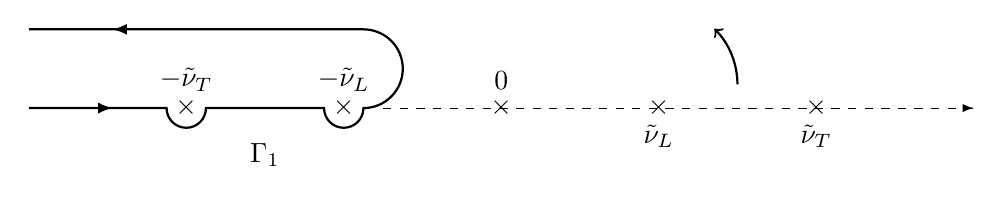
\begin{tikzpicture}
\node at (0,0) {$\times$};
\node at (0,0.35) {$0$};
\node at (2,0) {$\times$}; % Pole
\node at (4,0) {$\times$}; %pole
\node at (2,-0.36) {$\tilde{\nu}_L$};
\node at (4,-0.36) {$\tilde{\nu}_T$};

\node at (-2,0) {$\times$};
\node at (-4,0) {$\times$};
\node at (-2,0.36) {$-\tilde{\nu}_L$}; %pole
\node at (-4,0.36) {$-\tilde{\nu}_T$}; %pole
\node at (-3,-0.6) {$\Gamma_1$};

\draw[dashed, decoration={markings,
 mark=at position 1.0 with {\arrow{latex}}},
      postaction={decorate}] (-1.5,0) -- (6,0);
      
\draw[ thick, ->] (3.0,0.3) arc (0:45:1); %ici c'est les fleches 
  

\draw[thick, black, yshift=0pt,
decoration={ markings,  % This schema allows for fine-tuning the positions of arrows 
      mark=at position 0.1 with {\arrow{latex}},
      mark=at position 0.9 with {\arrow{latex}}},
      postaction={decorate}]
      (-6,0) -- (-4.25,0)  arc (-180:0:0.25) -- (-2.25,0)  arc (-180:0:0.25) -- (-1.75,0) arc(-90:90:0.5)  -- (-6,1);
\end{tikzpicture}
\caption{Contour $\Gamma_1$ in the case $\noncr$. The arrow shows the deformation of contour $\Gamma_0$ into $\Gamma_1$.}
\label{C4:gamma1noncr}
\end{figure}

\begin{figure}
\centering
\begin{subfigure}[b]{0.45\textwidth}
\begin{tikzpicture}[scale=0.8]
\node at (0,0) {$\times$};
\node at (0.35,0.35) {$0$};
\node at (0,1.5) {$\times$}; 
\node at (3,0) {$\times$}; 
\node at (-0.36,1) {$\tilde{\nu}_L$};
\node at (3,-0.36) {$\tilde{\nu}_T$};

\node at (0,-1.5) {$\times$};
\node at (-3,0) {$\times$};
\node at (-0.5,-1.5) {$-\tilde{\nu}_L$}; 
\node at (-3,0.36) {$-\tilde{\nu}_T$};
%\node at (-3,-0.6) {$\Gamma_1^a$};
%\node at (1,3) {$\Gamma_1^b$};

\draw[dashed, decoration={markings,
 mark=at position 1.0 with {\arrow{>}}},
      postaction={decorate}] (-2.5,0) -- (4,0);
      
\draw[dashed, decoration={markings,
 mark=at position 1.0 with {\arrow{>}}},
      postaction={decorate}] (0,-2.5) -- (0,4);

\draw[thick, black, yshift=0pt,
decoration={ markings,  % This schema allows for fine-tuning the positions of arrows 
      mark=at position 0.1 with {\arrow{latex}},
      mark=at position 0.9 with {\arrow{latex}}},
      postaction={decorate}]
      (-5,0) -- (-3.25,0)  arc (-180:0:0.25) -- (-2.75,0) arc(-90:90:0.5)  -- (-3.7,1);
      
\draw[thick, black, yshift=0pt,
decoration={ markings,  
      mark=at position 0.1 with {\arrow{latex}},
      mark=at position 0.9 with {\arrow{latex}}},
      postaction={decorate}]
      (-0.5,3.0) -- (-0.5,1.6) arc(0:180:-0.5)  -- (0.5,4);

\draw[ thick, ->] (-3,3)--(-3.7,3.7);
      
\draw[thick, black, yshift=0pt, decoration={ markings,  
      mark=at position 0.5 with {\arrow{latex}}},
      postaction={decorate}]
      (-3.7,1)arc(180:63.8:2.2);
\end{tikzpicture}
\caption{Intermediate contour $\Gamma_1$. The arrow shows the direction of the deformation.}
\end{subfigure}
~
\begin{subfigure}[b]{0.45\textwidth}
\begin{tikzpicture}[scale=0.8]
\node at (0,0) {$\times$};
\node at (0.35,0.35) {$0$};
\node at (0,1.5) {$\times$}; 
\node at (3,0) {$\times$}; 
\node at (-0.36,1) {$\tilde{\nu}_L$};
\node at (3,-0.36) {$\tilde{\nu}_T$};

\node at (0,-1.5) {$\times$};
\node at (-3,0) {$\times$};
\node at (-0.5,-1.5) {$-\tilde{\nu}_L$}; 
\node at (-3,0.36) {$-\tilde{\nu}_T$};
\node at (-3,-0.6) {$\Gamma_1^a$};
\node at (1,3) {$\Gamma_1^b$};

\draw[dashed, decoration={markings,
 mark=at position 1.0 with {\arrow{>}}},
      postaction={decorate}] (-2.5,0) -- (4,0);
      
\draw[dashed, decoration={markings,
 mark=at position 1.0 with {\arrow{>}}},
      postaction={decorate}] (0,-2.5) -- (0,3.5);

\draw[thick, black, yshift=0pt,
decoration={ markings,  % This schema allows for fine-tuning the positions of arrows 
      mark=at position 0.1 with {\arrow{latex}},
      mark=at position 0.9 with {\arrow{latex}}},
      postaction={decorate}]
      (-5,0) -- (-3.25,0)  arc (-180:0:0.25) -- (-2.75,0) arc(-90:90:0.5)  -- (-5,1);
      
\draw[thick, black, yshift=0pt,
decoration={ markings,  % This schema allows for fine-tuning the positions of arrows 
      mark=at position 0.1 with {\arrow{latex}},
      mark=at position 0.9 with {\arrow{latex}}},
      postaction={decorate}]
      (-0.5,3.5) -- (-0.5,1.6) arc(0:180:-0.5)  -- (0.5,3.5);
      
\end{tikzpicture}
\caption{Final contour $\Gamma_1=\Gamma_1^a \cup \Gamma_1^b$}
\end{subfigure}
\caption{Deformation of contour $\Gamma_0$ onto contour $\Gamma_1=\Gamma_1^a \cup \Gamma_1^b$ in the case $\crit$.}
\label{C4:gamma1cr}
\end{figure}

Similarly, in order to determine the action of operator $\mathbf{TM}$ on a simple pole, contour $\Gamma_0$ in \eqref{C4:B2TM} is deformed into contour $\partial \Omega_L$ for the L terms and $\partial \Omega_T$ for the T terms, both of these are visible in Fig.~\ref{C4:domegaT} for the case $\noncr$. Cauchy's residue theorem is applied, yielding, for $V \in \mathbb{C}^3$, Im$z\geq 0, \, z \notin \{\pm\tilde{\nu}_L,\pm\tilde{\nu}_T \}$, Im$\xi <0 $ with $z\in \mathbb{C} \backslash  \rbrack - \infty, -\nuti_L \rbrack$ :
\begin{equation}
\int_{\Gamma_0} \textbf{TM}(\xi,\zeta).\frac{V}{\zeta-z}\,d\zeta = \sum_{*=L,T} \frac{\textbf{tm}_*(z).V}{\xi-T_*(z)}\textbf{1}_{\Omega_*}(z)+\mathbf{T_p}(z,\xi).V
\label{C4:GaussTM}
\end{equation}
where $\textbf{1}_{\Omega_*}(z)=1$ if $z\in \Omega_*$ and $\textbf{1}_{\Omega_*}(z)=0$ elsewhere and
\begin{equation}
\mathbf{T_p}(z,\xi)= \frac{1}{2i\pi} \sum_{*=L,T} \int_{\partial \Omega_*} D_*(\xi,\zeta) .\dfrac{\textbf{tm}_*(\zeta)}{\zeta-z}\, d\zeta
\label{C4:defTp}
\end{equation}

\begin{figure}
\centering
\begin{subfigure}[b]{0.45\textwidth}
   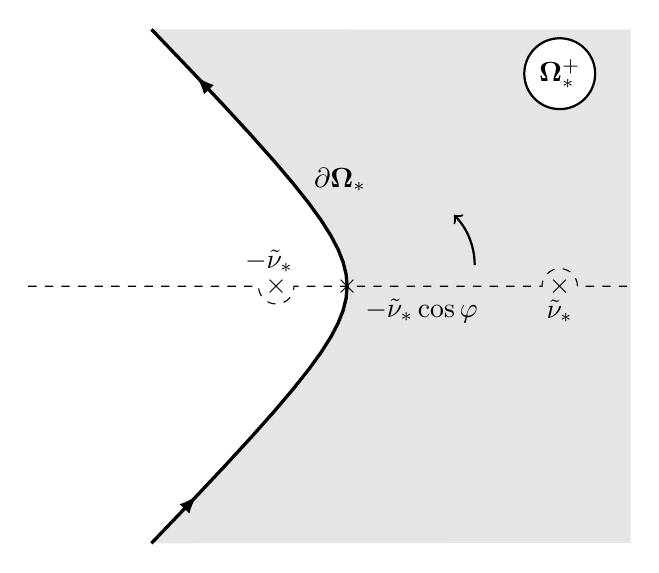
\begin{tikzpicture}[scale=0.9]
% Remplissage espace Omega_0
\fill [color=gray!20]
(3,-3.62) -- plot [domain=-2:2] ({-cosh(\x)},{sinh(\x)}) -- (3,3.62);
%(3,0) -- plot [domain=0:2] ({-cosh(\x)},{sinh(\x)}) -- (3,3.62) -- cycle;
\fill[color=white] (2,3) circle (0.5);
%\fill [color=white] (2,0) circle (0.25);

\node at (2,0) {$\times$};
\node at (2,-0.35) {$\tilde{\nu}_*$};
\node at (-2,0) {$\times$};
\node at (-1,0) {$\times$};
\node at (-2.1,0.35) {$-\tilde{\nu}_*$}; 
\draw[dashed]
      (-5.5,0) -- (-2.25,0)  arc (-180:0:0.25)  -- (1.75,0)arc (180:0:0.25) -- (3,0); 
\draw[black, very thick,decoration={ markings,  
      mark=at position 0.1 with {\arrow{latex}},
      mark=at position 0.9 with {\arrow{latex}}},
      postaction={decorate}][domain=-2:2] plot({-cosh(\x)}, {sinh(\x)});
\node at (-1.1,1.5) {$\mathbf{\partial \Omega_*}$};
\node at (0.05,-0.35) {$-\nuti_*\cos \varphi$};

% Espace Omega_0
\draw[thick] (2,3) circle (0.5);
\node at (2,3) {$\mathbf{\Omega_*^+}$};

\draw[ thick, ->] (0.8,0.3) arc (0:45:1); %ici c'est les fleches 
%\node at (1.2,0.8) {$\mathbf{\mathcal{F}_2}$}; 
\end{tikzpicture}
\caption{Contour $\partial \Omega_*$ and domain $\Omega_*^+$ in the case $\noncr$. The curved arrow shows deformation of contour $\Gamma_0$ onto $\partial \Omega_*$.}
\label{C4:domegaT}     
\end{subfigure}
\hfill
\begin{subfigure}[b]{0.45\textwidth}
   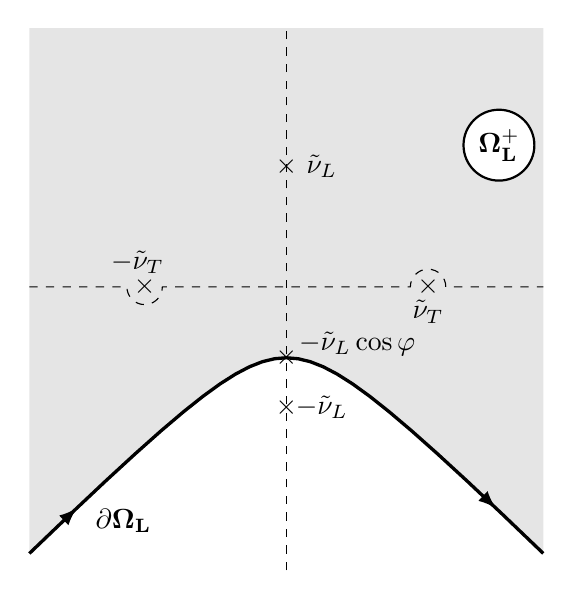
\begin{tikzpicture}[scale=0.9]
\fill [color=gray!20]
(-3.6269,3.65) -- plot [domain=-2:2] ({sinh(\x)},{-cosh(\x)}) -- (3.6269,3.65) ;
\fill[color=white] (3,2) circle (0.5);
\node at (2,0) {$\times$}; 
\node at (0,-1) {$\times$};
\node at (0,1.7) {$\times$};
\node at (0,-1.7) {$\times$};
\node at (2,-0.35) {$\tilde{\nu}_T$};
\node at (-2,0) {$\times$};
\node at (-2.1,0.35) {$-\tilde{\nu}_T$}; 
\draw[dashed]
      (-3.6269,0) -- (-2.25,0)  arc (-180:0:0.25)  -- (1.75,0)arc (180:0:0.25) -- (3.6269,0); % ca c'est l'axe
\draw[dashed] (0,-4) -- (0,3.65);
% Hyperbole (contour  partial_Omega_0 )
\draw[black, very thick,decoration={ markings,  % This schema allows for fine-tuning the positions of arrows 
      mark=at position 0.1 with {\arrow{latex}},
      mark=at position 0.9 with {\arrow{latex}}},
      postaction={decorate}][domain=-2:2] plot({sinh(\x)},{-cosh(\x)});
\node at (1,-0.8) {$-\nuti_L\cos\varphi$};
\node at (0.5,1.7) {$\nuti_L$};
\node at (0.5,-1.7) {$-\nuti_L$};
\node at (-2.3,-3.3) {$\mathbf{\partial \Omega_L}$};

% Espace Omega_0
\draw[thick] (3,2) circle (0.5);
\node at (3,2) {$\mathbf{\Omega_L^+}$};
\end{tikzpicture}
\caption{Contour $\partial \Omega_L$ and domain $\Omega_L^+$ in the case $\crit$.}
\label{C4:domegaL}
\end{subfigure}
\caption{Domains $\Omega_*$ and contours $\partial \Omega_*$ in cases $\noncr$ and $\crit$.}
\label{C4:domega0}
\end{figure}

In the case where $\crit$, $\partial \Omega_L$ is visble in Fig.~\ref{C4:domegaL}. During the deformation of contour $\Gamma_0$ into contour $\partial\Omega_L$, the pole $z$ is not crossed  and therefore does not contribute to the integral. However, if there exists $\zeta_0 \in \Omega_L^+$ such that $T_L(\zeta_0)=\xi$ and Im$\zeta_0<0$, then pole $\zeta_0$ is crossed during this deformation. Suppose that $\zeta_0=\nuti_L\cos\theta_0=\nuti_L\cos(\theta_0'+i\theta_0'')$ and $\xi=T_L(\zeta_0)=\nuti_L\cos(\theta_0+\phiti)$ with $\nuti_L=i\eta_L \in i\mathbb{R}$, we then have :
\begin{equation}
\rm Im \zeta_0=\eta_L\cos\theta_0'\cosh\theta_0''  
\end{equation}
Combining the facts that Im$\zeta_0<0$ and $\zeta_0 \in \Omega_L^+$ gives
\begin{equation}
\dfrac{\pi}{2}<\theta_0'<\pi-\phiti
\label{C4:condcr}
\end{equation}
Condition \eqref{C4:condcr} makes sense if and only if $\phiti<\dfrac{\pi}{2}$. From hereon after, we will suppose that this is not the case (this restriction is only made when $\crit$). In practice, this is not too restrictive since, as explained in \ref{Chapter5:sing_part}, the spectral functions method is less accurate for small values of $\phiti$. Therefore, when $\crit$, Cauchy's residue theorem yields, for $V \in \mathbb{C}^3$, Im$z\geq 0, \, z \notin \{\pm\tilde{\nu}_L,\pm\tilde{\nu}_T \}$, Im$\xi <0 $ with $z\in \mathbb{C} \backslash ( \rbrack - \infty, -\nuti_L \rbrack\cup \lbrack \nuti_L,+i\infty\lbrack)$ :
\begin{equation}
\int_{\Gamma_0} \textbf{TM}(\xi,\zeta).\frac{V}{\zeta-z}\,d\zeta = \frac{\textbf{tm}_T(z).V}{\xi-T_T(V)}\textbf{1}_{\Omega_T}(z)+\mathbf{T_p}(z,\xi).V
\label{C4:GaussTMcr}
\end{equation}
with $\mathbf{T_p}$ defined by \eqref{C4:defTp}.

It is important to note that in all the aforementioned contour deformations, no branch points of the integrands are crossed. Therefore, it is assumed that Croisille and Lebeau's \cite{CroisilleLebeau} proof that $\mathbf{D_p}(z,\cdot)$ and $\mathbf{T_p}(z,\cdot)$ belong to a special class of functions $\mathcal{H}^3$ can be adapted to the 3D case. It will therefore be assumed that in the case $\noncr$, $\mathbf{D_p}(z,\cdot) \in \mathcal{H}^3$ and $\mathbf{T_p}(z,\cdot) \in \mathcal{H}^3$ and in the case $\crit$, $\mathbf{D_p}(z,\cdot) \in \tilde{\mathcal{H}}^3$ and $\mathbf{T_p}(z,\cdot) \in \mathcal{H}^3$. $\mathcal{H}$ and $\tilde{\mathcal{H}}$ are defined hereafter
\begin{definition}
\label{C4:defH}
$\mathcal{H}$ is the space of the functions f analytical in $\mathbb{C}\backslash \rbrack -\infty,-\nuti_L\rbrack$ such that $\forall \epsilon \in \rbrack0,\pi \lbrack, f(e^{i\epsilon} \cdot)\in H^+$, where $H^+$ is defined in Def.~\ref{defHpl}.
\end{definition}
\begin{definition}
\label{C4:defHcrit}
$\tilde{\mathcal{H}}$ is the space of the functions f analytical in  $\mathbb{C} \backslash ( \, \rbrack - \infty, -\nuti_T \rbrack \cup \lbrack \nuti_L,+i\infty \lbrack \,)$ such that $\forall \epsilon \in \rbrack0,\pi \lbrack, f(e^{i\epsilon} \cdot)\in H^+$, where $H^+$ is defined in Def.~\ref{defHpl}.
\end{definition}

The recursive procedure used to extract all the poles and corresponding residues of the spectral functions is analogous to the one described in \ref{C3:singpart} and will not be repeated here. 
%Let us now extract all the poles and corresponding residues of the spectral functions, using system \eqref{C4:equationsintegrales} and results \eqref{C4:GaussDM} and \eqref{C4:GaussTM}. We begin with the following decomposition, for Im $\xi \le 0$ : 
%\begin{equation}
%\Sigma_j(\xi)= \frac{V_j^{(0)}}{\xi-Z^{(0)}_j}+X'_j(\xi)
%\label{C4:extraction1}
%\end{equation}
%where $V_j^{(0)}$ are to be determined, $X'_j$ is an unknown function and
%\begin{subequations}
%\begin{equation}
%Z_1^{(0)}=\nu_{\alpha} \cos \theta_{inc}\cos\delta_{inc}=\nuti_{\alpha}\cos\theta_{inc},
%\end{equation}
%\begin{equation}
%Z_2^{(0)}=\nu_{\alpha} \cos(\varphi-\theta_{inc})\cos\delta_{inc}=\nuti_{\alpha}\cos(\varphi-\theta_{inc}).
%\end{equation}
%\end{subequations}
%Substituting \eqref{C4:extraction1} into \eqref{C4:equationsintegrales} and applying \eqref{C4:GaussDM} yields
%\begin{eqnarray}
%\left\{
%\begin{array}{l}
%\textbf{DM}(X'_1)+\textbf{TM}(X'_2)+\textbf{TM}(\frac{V_2^{(0)}}{\xi-Z_2^{(0)}})=\frac{W^1_{\alpha}}{\xi-Z_1^{(0)}}-\frac{\textbf{dm}(Z_1^{(0)}).V_1^{(0)}}{\xi-Z_1^{(0)}}-\mathbf{D_p}(Z_1^{(0)},\xi).V_1^{(0)} \\
%~
%\\
%\textbf{TM}(X'_1)+\textbf{DM}(X'_2)+\textbf{TM}(\frac{V_1^{(0)}}{\xi-Z_1^{(0)}})=\frac{W^2_{\alpha}}{\xi-Z_2^{(0)}}-\frac{\textbf{dm}(Z_2^{(0)}).V_2^{(0)}}{\xi-Z_2^{(0)}}-\mathbf{D_p}(Z_2^{(0)},\xi).V_2^{(0)} 
%\end{array}
%\right.
%\label{C4:mille}
%\end{eqnarray}
%The singular terms in the right-hand side of this system are eliminated by setting
%\begin{equation}
%V_j^{(0)}=\textbf{dm}^{-1}(Z_j^{(0)}).W_j^{\alpha}
%\end{equation}
%In all the following, we will suppose that we have det$(\mathbf{dm}) \neq 0$. Applying \eqref{C4:GaussTM} reveals two new poles, leading to a second decomposition 
%\begin{equation}
%X'_j=X''_j+\frac{V_{j,L}^{(1)}}{\xi-Z_{j,L}^{(1)}}+\frac{V_{j,T}^{(1)}}{\xi-Z_{j,T}^{(1)}}
%\end{equation}
%where, for $*=L,T$ 
%\begin{equation}
%Z_{j,*}^{(1)}=T_*(Z_{3-j}^{(0)})
%\end{equation}
%and $V_{j,*}^{(1)}$ remain to be determined. Once again, they are chosen so as to eliminate the singular terms in the right-hand side of the system :
%\begin{equation}
%V_{j,*}^{(1)}=-\mathbf{dm}^{-1}(T_*(Z_{j}^{(0)})).\mathbf{tm_*}(Z_{3-j}^{(0)}).V_{3-j}^{(0)}
%\end{equation}
%These steps are repeated recursively as long as $\textbf{1}_{\Omega_L}(Z_{j,*}^{(k)}=1$ and $\textbf{1}_{\Omega_T}(Z_{j,*}^{(k)}=1$. 
In the end, we have, for  $\mbox{Im} \xi <0$
\begin{equation}
\Sigma_j(\xi)=Y_j(\xi)+X_j(\xi) \label{C4:decomp}
\end{equation}
where, when $\noncr$ :
\begin{equation}
Y_j(\xi)=\sum_k \sum_{*=L,T} \frac{V_{j,*}^{(k)}}{\xi-Z_{j,*}^{(k)}}
\label{C4:yj},
\end{equation}
with
\begin{equation}
\begin{matrix}
Z_{1}^{(0)}=\nuti_{\alpha} \cos \theta_{inc},  & Z_{2}^{(0)}=\nuti_{\alpha} \cos(\varphi-\theta_{inc}) \\
Z_{j,L}^{(k+1)}= T_L(Z_{3-j,*}^{(k)}) &Z_{j,T}^{(k+1)}= T_T(Z_{3-j,*}^{(k)}) 
\end{matrix}
\label{C4:poles}
\end{equation}
and
\begin{equation}
\begin{matrix}
V_{j}^{(0)}=\textbf{dm}^{-1}(Z_{j}^{(0)}).W_j^{\alpha}\\
V_{j,L}^{(k+1)}=-\textbf{dm}^{-1}(Z_{j,*}^{(k+1)}).\textbf{tm}_L(Z_{3-j,*}^{(k)}).V_{3-j,*}^{(k)}.\textbf{1}_{\Omega_L}(Z_{3-j,*}^{(k)}) \\ 
V_{j,T}^{(k+1)}=-\textbf{dm}^{-1}(Z_{j,*}^{(k+1)}).\textbf{tm}_T(Z_{3-j,*}^{(k)}).V_{3-j,*}^{(k)}.\textbf{1}_{\Omega_T}(Z_{3-j,*}^{(k)}) 
\end{matrix}
\label{C4:residus}
\end{equation}
an when $\crit$,
\begin{equation}
Y_j(\xi)=\sum_k \frac{V_{j,T}^{(k)}}{\xi-Z_{j,T}^{(k)}}
\label{C4:yjcr},
\end{equation}
with
\begin{equation}
\begin{matrix}
Z_{1}^{(0)}=\nuti_T \cos \theta_{inc},\\ 
Z_{2}^{(0)}=\nuti_T \cos(\varphi-\theta_{inc})\\
Z_{j,T}^{(k+1)}= T_T(Z_{3-j,T}^{(k)}) 
\end{matrix}
\label{C4:polescr}
\end{equation}
and
\begin{equation}
\begin{matrix}
V_{j}^{(0)}=\textbf{dm}^{-1}(Z_{j}^{(0)}).W_j^{\alpha}\\
V_{j,T}^{(k+1)}=-\textbf{dm}^{-1}(Z_{j,*}^{(k+1)}).\textbf{tm}_T(Z_{3-j,*}^{(k)}).V_{3-j,*}^{(k)}.\textbf{1}_{\Omega_T}(Z_{3-j,*}^{(k)}) 
\end{matrix}
\label{C4:residuscr}
\end{equation}
As in \ref{C3:singpart}, the recursive procedure stops when no more poles can be found by deforming contour $\Gamma_0$ into $\partial \Omega_L$ or $\partial \Omega_T$. In the 2D case, Croisille and Lebeau \cite{CroisilleLebeau} have shown that this defines a finite number of poles. The sequence of poles generated in the 3D case being similar to the ones generated in the 2D case (parameters $\nu_L$ and $\nu_T$ in the 2D case are replaced by parameters $\nuti_L$ and $\nuti_T$), their demonstration is still valid here. 
%We will now prove that this is still true when $\crit$. Physically, this means that an incident ray exits the wedge after a finite number of reflections and mode conversions.
%\begin{lemma}
%The number of poles defined recursively by \eqref{C4:poles}, is finite.
%\label{C4:finipoles}
%\end{lemma}
%\paragraph*{Proof.} To prove lemma \ref{C4:finipoles}, it is sufficient to prove that and infinite sequence $(z_l)_{l\geq0}$ of the form
%\begin{equation}
%z_0 \in \mathbb{C}, \hspace{1em} z_{l+1}=T_{\nuti_l}(z_l), \hspace{1em} z_l\in\Omega_{\nuti_l}, \hspace{1em} \nuti_l=\nuti_L=i\eta_L \rm or \nuti_l=\nuti_T
%\end{equation}
%does not exist. Suppose we have :
%\begin{equation}
%\begin{split}
%z_l&=\nuti_l\cos\theta_l=\nuti_l\cos(\theta_1^l+i\theta_2^l)\\
%&=\nuti_l(\cos\theta_1^l\cosh\theta_2^l-i\sin\theta_1^l\sinh\theta_2^l
%\end{split}
%\end{equation}
%with $0\leq \theta_1^l\leq \pi-\phiti$. Then, if $\nuti_l=\nuti_T$ :
%\begin{equation}
%\begin{split}
%\rm Re(T_T(z_l))&=\nuti_T\cos(\theta_1^l+\phiti)\cosh\theta_2^l\\
%&\leq\nuti_T(\cos\theta_1^l-\varepsilon_0)\cosh\theta_2^l\leq \rm Re(z_l)-\nuti_T \varepsilon_0
%\end{split}
%\end{equation}
%where $\varepsilon_0>0$ depends only of $\phiti$. If $\nuti_l=\nuti_L=i\eta_L$, then
%\begin{equation}
%\begin{split}
%\rm Im(T_L(z_l))&=\eta_L\cos(\theta_1^l+\phiti)\cosh\theta_2^l\\
%&\leq\eta_L(\cos\theta_1^l-\varepsilon_0)\cosh\theta_2^l\leq \rm Re(z_l)-\eta_L \varepsilon_0
%\end{split}
%\end{equation}
%In both cases, if the number of points $z_l$ is infinite, then $|z_l| \rightarrow +\infty$, implying $|\theta_2^l| \rightarrow +\infty$ and
%\begin{equation}
%\cosh\theta_2^l \sim |\sinh\theta_2^l| \sim \frac{1}{2} e^{|\theta_2^l|}
%\end{equation}
%which in turn, implies
%\begin{equation}
%|\rm arg \, z_l| \sim \theta_1^l \hspace{1em}\rm and \hspace{1em}|\rm arg \,z_{l+1}| \sim \theta_1^l+\phiti \sim \theta_1^{l+1} \Rightarrow \theta_1^l \rightarrow +\infty
%\end{equation}
%This is impossible. Therefore, the sequence $(z_l)_{l\geq 0}$ is necessarily finite.
%\paragraph*{}
We have thus extracted all the poles from the spectral functions and have computed them analytically, along with their corresponding residues.

\subsection{Regular Part}
\label{C4:regpart}
The singular parts $Y_j$ of the spectral functions having been determined, two new functions $X_1$ and $X_2$ are defined by \eqref{C4:decomp}. In the following, a numerical approximation method for $X_j$ is proposed. In order to do so, a system of functional equations solved by $X_1, X_2$ is derived by subtracting vector 
\begin{equation}
\begin{pmatrix}
\textbf{DM}(Y_1)+\textbf{TM}(Y_2) \\
\textbf{TM}(Y_1)+\textbf{DM}(Y_2)
\end{pmatrix},
\end{equation}
from both sides of \eqref{C4:equationsintegrales}, where $Y_1$ and $Y_2$ are given by equations \eqref{C4:yj} to \eqref{C4:residuscr} :
\begin{equation}
\left\{ 
\begin{matrix}
\mathbf{DM}(X_1)(\xi)+\textbf{TM}(X_2)(\xi)=u_1(\xi)\\
\textbf{TM}(X_1)(\xi)+\textbf{DM}(X_2)(\xi)=u_2(\xi)
\end{matrix}
\right.,
\label{C4:regparteqn}
\end{equation}
with, for $j=1,2$
\begin{equation}
u_j(\xi)=-\sum_k \sum_{*=L,T} \left[ \mathbf{D_p}(Z_{j,*}^{(k)},\xi).V_{j,*}^{(k)}+\mathbf{T_p}(Z_{3-j,*}^{(k)},\xi).V_{3-j,*}^{(k)}\right]
\label{C4:scndmembre}
\end{equation}
It is assumed that Croisille and Lebeau's \cite{CroisilleLebeau} proof that this system has a unique solution $(X_1,X_2)$ in $\mathcal{H}^3$ (defined in Def.~\ref{C4:defH} is $\noncr$ and Def.~\ref{C4:defHcrit} if $\crit$) can be adapted to the 3D case. Once again, a numerical approximation of the regular parts $X_j$ will be computed using the Galerkin collocation method. The functional space $\mathcal{H}$ is approached by the finite-dimension subspace generated by basis functions $(\varphi_k)_{1 \leq k \leq 2N}$ defined by \eqref{Gal_basis}, with $(a_k)_{1 \leq k \leq 2N} \in \lbrack \nuti_L, + \infty \lbrack^N$ if $\noncr$ and $(a_k)_{1 \leq k \leq N} \in \lbrack \nuti_T, + \infty \lbrack^N ,\; \; (a_k)_{N+1\leq k \leq 2N} \in \rbrack -i\infty, -\nuti_L\rbrack^N$ if $\crit$. Functions $X_j$ are approximated in this space by :
\begin{equation}
 X_j(\xi) \approx \sum_{k=1}^N \tilde{X}_j^k \varphi_k(\xi) ,\hspace{1em} \tilde{X}_j^k \in \mathbb{C}^3
 \label{C4:Xj}
\end{equation}
Approximation \eqref{C4:Xj} is substituted into \eqref{C4:regparteqn} and the variable change $\zeta=iy$ is applied in the resulting system. This system is then evaluated at $\xi=b_1,...,b_{2N}$, leading to a linear system of equations which can be written in matrix form :
\begin{eqnarray}
\begin{pmatrix}
\mathbb{D}&\mathbb{T}\\
\mathbb{T}&\mathbb{D}
\end{pmatrix}
\begin{pmatrix}
\mathbb{X}_1 \\
\mathbb{X}_2
\end{pmatrix}
=
\begin{pmatrix}
\mathbb{U}_1 \\
\mathbb{U}_2
\end{pmatrix}
\Leftrightarrow
\left\{
\begin{array}{l}
(\mathbb{D}+\mathbb{T})(\mathbb{X}_1+\mathbb{X}_2)= \mathbb{U}_1+\mathbb{U}_2 \\
(\mathbb{D}-\mathbb{T})(\mathbb{X}_1-\mathbb{X}_2)= \mathbb{U}_1-\mathbb{U}_2
\end{array}
	\right.,
\label{C4:systmat}
\end{eqnarray}
where matrices $(6N\times 6N)$ are defined by $3\times3$ blocks:
\begin{equation}
\begin{split}
\mathbb{D}_{lk}&=\int_{-\infty}^{+\infty} \textbf{DM}(b_l,iy)e_{a_k}(y) \, dy =\frac{1}{2i\pi} \int_{-\infty}^{+\infty} \frac{\mathbf{dm}}{b_l-iy} 
%\begin{pmatrix}
%-1&A(iy) \\
%B(iy)&-1
%\end{pmatrix}
\sqrt{\frac{a_k}{\pi}}\frac{1}{y-ia_k} \, dy \\
&=- \frac{\sqrt{a_k}}{2\pi \sqrt{\pi}}
\begin{pmatrix}
\mathcal{D}_1(a,b) &\mathcal{D}_2^T(a,b) &0\\
-\mathcal{D}_2^L(a,b) &\mathcal{D}_1(a,b)&-\mathcal{D}_3^L(a,b)\\
0&\mathcal{D}_3^T(a,b)&\mathcal{D}_1(a,b)
\end{pmatrix}=\frac{\sqrt{a_k}}{2\pi \sqrt{\pi}}\mathbb{D}(a_k,b_l)
\end{split}
\label{C4:Dab}
\end{equation}
where functions $e_{a_k}$ are defined by \eqref{Galerkin_basis} and the explicit expressions of coefficients of matrix $\mathbb{D}(a,b)$ and their values are computed in appendix \ref{finalD3D}. The other matrices involved are, for $1\leq l,k \leq 2N$
\begin{equation}
\begin{split}
\mathbb{T}_{lk}&=\int_{-\infty}^{+\infty} \textbf{TM}(b_l,iy)e_{a_k}(y) \, dy 
=\frac{1}{2i\pi} \int_{-\infty}^{+\infty} \sum_{*=L,T} \frac{\textbf{tm}_* (iy, \mbox{sgn} \sin \varphi)}{b_l-T_*(iy)} \sqrt{\frac{a_k}{\pi}}\frac{1}{y-ia_k}\,dy \\
&=\frac{1}{2i\pi}\sqrt{\frac{a_k}{\pi}}\sum_{*=L,T} \int_{-\infty}^{+\infty} \frac{\textbf{tm}_*(iy,\epsilon)}{\lbrack b_l-(iy \cos \varphi +  \zeta_*(iy)| \sin \varphi|)\rbrack(y-ia_k)} \, dy,
\end{split}
\end{equation}
where $\epsilon= \mbox{sgn}( \sin \varphi)$. Let us define
\begin{equation}
\mathbb{T}_{lk}=\frac{1}{2i\pi}\sqrt{\frac{a_k}{\pi}}
\sum_{*=L,TH,TV}
\begin{pmatrix}
\mathcal{T}_1^*(a,b) &  \mathcal{T}_2^*(a,b) &\mathcal{T}_3^*(a,b) \\
\mathcal{T}_4^*(a,b) &\mathcal{T}_5^*(a,b)&\mathcal{T}_6^*(a,b)\\
\mathcal{T}_7^*(a,b)&\mathcal{T}_8^*(a,b)&\mathcal{T}_9^*(a,b)
\end{pmatrix}
=\frac{1}{2i\pi}\sqrt{\frac{a_k}{\pi}}\mathbb{T}(a_k,b_l)
\label{Tab}
\end{equation}
The explicit expressions of operators $\mathcal{T}_i^*, 1\leq i\leq9, *=L,TH,TV$ and their values are computed in \ref{finalT3D}. Finally:
\begin{equation}
\mathbb{X}_j=
\begin{pmatrix}
\tilde{X}_j^1\\
\vdots \\
\tilde{X}_j^{2N}
\end{pmatrix}
\hspace{3em}
\mathbb{U}_j=
\begin{pmatrix}
u_j(b_1)\\
\vdots \\
u_j(b_{2N})
\end{pmatrix}
\end{equation}
where $u_j(\xi)$ is given by \eqref{C4:scndmembre}. The same considerations as those made in \ref{C3:regpart} lead to an expression of $u_j$ with respect to operators $\mathbb{D}(\cdot,\cdot)$ and $\mathbb{T}(\cdot,\cdot)$ :
\begin{equation}
u_j(\xi)=-\frac{1}{2i\pi}\sum_{k}\sum_{*=L,T}\left(i\mathbb{D}(-Z_{j,*}^{(k)},\xi).V_{j,*}^{(k)}+\mathbb{T}(-Z_{3-j,*}^{(k)},\xi).V_{3-j,*}^{(k)} \right) +\frac{W_j^{\alpha}}{\xi-Z_j^{(0)}}
\label{C4:uDT}
\end{equation}

 Using these results, the linear system \eqref{C4:systmat} is implemented and solved numerically using the C++ library Eigen, and an evaluation of the regular part of the spectral functions is obtained. However, for values of $\xi$ lying in certain parts of the complex plane, this evaluation is not sufficiently accurate. The technique used to solve this problem is called the propagation of the solution.
 
\subsection{Propagation of the solution}
\label{C4:propag}
The method called propagation of the solution is used to propagate the accuracy of the numerical approximation of the regular functions $X_1$ and $X_2$ from parts of the complex plane where they are evaluated accurately to parts of the complex plane where they are not.

\begin{figure}[h]
	\centering
	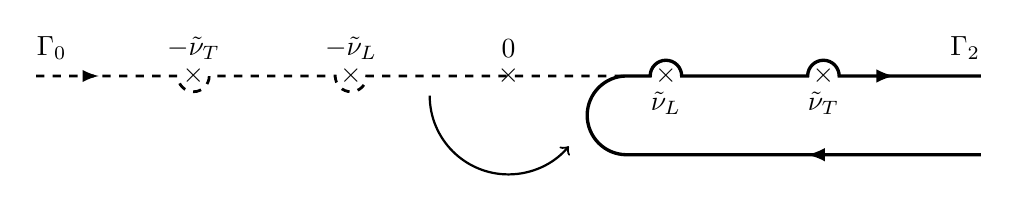
\begin{tikzpicture}
	\node at (0,0) {$\times$};
	\node at (0,0.35) {$0$};
	\node at (2,0) {$\times$}; % Pole
	\node at (2,-0.35) {$\nuti_L$};
	\node at (4,0) {$\times$};
	\node at (4,-0.35) {$\nuti_T$};
	\node at (-2,0) {$\times$};
	\node at (-2,0.35) {$-\nuti_L$};
	\node at (-4,0) {$\times$};
	\node at (-4,0.35) {$-\nuti_T$};
	\node at (5.8,0.35) {$\Gamma_2$};
	\node at (-5.8,0.35) {$\Gamma_0$};
	\draw[very thick, black,yshift=0pt,
	decoration={ markings,
		mark=at position 0.2 with {\arrow{latex}},
		mark=at position 0.9 with {\arrow{latex}}},
	postaction={decorate}]
	(6,-1) -- (1.5,-1)  arc (90:-90:-0.5) -- (1.8,0) arc (180:0:0.2) -- (3.8,0) arc (180:0:0.2) -- (6,0);
	
	\draw[dashed, line width = 1pt,yshift=0pt,
	decoration={ markings,
		mark=at position 0.1 with {\arrow{latex}}},
	postaction={decorate}]
	(-6,0) -- (-4.2,0) arc (-180:0:0.2) -- (-2.2,0)  arc (-180:0:0.2)  -- (1.5,0);
	
	\draw[ thick, ->] (-1,-0.25) arc (180:320:1);
	\end{tikzpicture}
	\caption{Integration contour $\Gamma_2$ in the case $\noncr$. The curved arrow indicates the contour deformation from $\Gamma_0$ to $\Gamma_2$.}
	\label{C4:contour2}
\end{figure}

The first step of this procedure is to deform contour $\Gamma_0$ in operator $\mathbf{DM}$ into contour $\Gamma_2$ in \eqref{C4:regparteqn}. Contour $\Gamma_2$ is visible on Fig.~\ref{C4:contour2} for the case $\noncr$ and in Fig.~\ref{C4:contour2crit} for the case $\crit$. During this deformation, the half-plane Im$\xi<0$ is crossed (with the exception of branch $\lbrack -\nuti_L,-\infty \lbrack$ in the case $\crit$). The contribution of poles $\zeta=\xi$, Im$\xi<0$ crossed during this contour deformation is given by Cauchy's residue formula :
\begin{equation}
\int_{\Gamma_0} \textbf{DM}(\xi,\zeta)X_j(\zeta)\, d\zeta = \int_{\Gamma_2}  \textbf{DM}(\xi,\zeta)X_j(\zeta)\, d\zeta + \textbf{dm}(\xi).X_j(\xi)
\label{C4:DM2}
\end{equation}

\begin{figure}
\centering
\begin{subfigure}[b]{0.45\textwidth}
	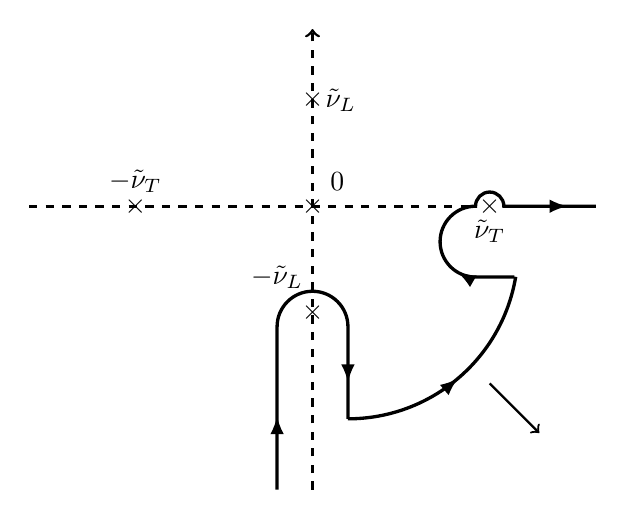
\begin{tikzpicture}[scale=0.9]
	\node at (0,0) {$\times$};
	\node at (0.35,0.35) {$0$};
	\node at (0,1.5) {$\times$}; % Pole
	\node at (0.4,1.5) {$\nuti_L$};
	\node at (2.5,0) {$\times$};
	\node at (2.5,-0.35) {$\nuti_T$};
	\node at (0,-1.5) {$\times$};
	\node at (-0.5,-1) {$-\nuti_L$};
	\node at (-2.5,0) {$\times$};
	\node at (-2.5,0.35) {$-\nuti_T$};
%	\node at (5.8,0.35) {$\Gamma_2^a$};
%	\node at (1,-4) {$\Gamma_2^b$};
%	\node at (-5.8,0.35) {$(\Gamma_0)$};
	
	\draw[very thick, black,yshift=0pt,
	decoration={ markings,  % This schema allows for fine-tuning the positions of arrows 
		mark=at position 0.2 with {\arrow{latex}},
		mark=at position 0.9 with {\arrow{latex}}},
	postaction={decorate}]
	(2.85,-1) -- (2.3,-1)  arc (90:-90:-0.5)  -- (2.3,0) arc (180:0:0.2) -- (4,0);
	
	\draw[very thick, black,yshift=0pt,
	decoration={ markings,  % This schema allows for fine-tuning the positions of arrows 
		mark=at position 0.2 with {\arrow{latex}},
		mark=at position 0.9 with {\arrow{latex}}},
	postaction={decorate}]
	(-0.5,-4) -- (-0.5,-1.7) arc (0:-180:-0.5) -- (0.5,-3);
	
	\draw[very thick, black,yshift=0pt,
	decoration={ markings,mark=at position 0.5 with {\arrow{latex}}},
	postaction={decorate}]
	(0.5,-3) arc (-90:-9.5:2.4);
	
	\draw[dashed, line width =1pt, yshift=0pt,
	decoration={ markings,mark=at position 1 with {\arrow{>}}},
	postaction={decorate}]
	(0,-4)--(0,2.5);
	
%	\draw[dashed, line width = 1pt,yshift=0pt,
%	decoration={ markings,mark=at position 0.1 with {\arrow{latex}}},
%	postaction={decorate}]
%	(-6,0) -- (-3.2,0) arc (-180:0:0.2) -- (2.8,0)arc (180:0:0.2);

\draw[dashed, line width = 1pt,yshift=0pt]
	(-4,0) -- (2.3,0);
	
	\draw[ thick, ->] (2.5,-2.5)--(3.2,-3.2);
	
	\end{tikzpicture}
	\caption{Intermediate contour $\Gamma_2$. The arrow shows the direction of the deformation.}
\end{subfigure}
~
\begin{subfigure}[b]{0.45\textwidth}
	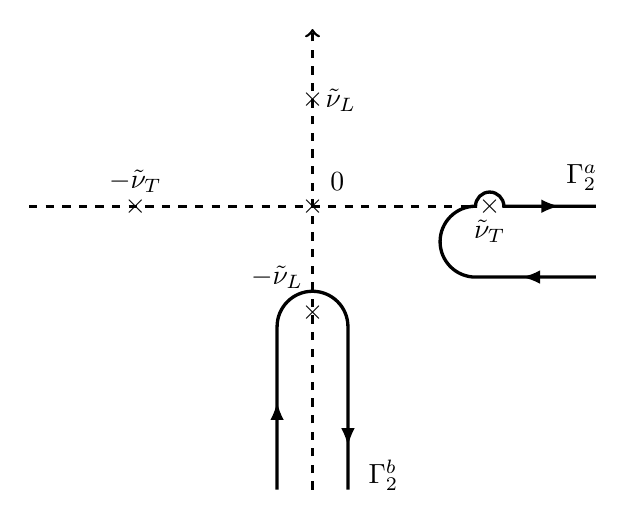
\begin{tikzpicture}[scale=0.9]
	\node at (0,0) {$\times$};
	\node at (0.35,0.35) {$0$};
	\node at (0,1.5) {$\times$}; % Pole
	\node at (0.4,1.5) {$\nuti_L$};
	\node at (2.5,0) {$\times$};
	\node at (2.5,-0.35) {$\nuti_T$};
	\node at (0,-1.5) {$\times$};
	\node at (-0.5,-1) {$-\nuti_L$};
	\node at (-2.5,0) {$\times$};
	\node at (-2.5,0.35) {$-\nuti_T$};
	\node at (3.8,0.4) {$\Gamma_2^a$};
	\node at (1,-3.8) {$\Gamma_2^b$};
%	\node at (-4.8,0.35) {$(\Gamma_0)$};
	
	\draw[very thick, black,yshift=0pt,
	decoration={ markings,  
		mark=at position 0.2 with {\arrow{latex}},
		mark=at position 0.9 with {\arrow{latex}}},
	postaction={decorate}]
	(4,-1) -- (2.3,-1)  arc (90:-90:-0.5)  -- (2.3,0) arc (180:0:0.2) -- (4,0);
	
	\draw[very thick, black,yshift=0pt,
	decoration={ markings, 
		mark=at position 0.2 with {\arrow{latex}},
		mark=at position 0.9 with {\arrow{latex}}},
	postaction={decorate}]
	(-0.5,-4) -- (-0.5,-1.7) arc (0:-180:-0.5) -- (0.5,-4);
	
	\draw[dashed, line width =1pt, yshift=0pt,
	decoration={ markings,mark=at position 1 with {\arrow{>}}},
	postaction={decorate}]
	(0,-4)--(0,2.5);
	
%	\draw[dashed, line width = 1pt,yshift=0pt,
%	decoration={ markings,mark=at position 0.1 with {\arrow{latex}}},
%	postaction={decorate}]
%	(-6,0) -- (-3.2,0) arc (-180:0:0.2) -- (2.8,0)arc (180:0:0.2);

	\draw[dashed, line width = 1pt,yshift=0pt]
	(-4,0) -- (2.3,0);
	
	\end{tikzpicture}
	\caption{Final contour $\Gamma_2=\Gamma_2^a\cup\Gamma_2^b$}
\end{subfigure}
\caption{Deformation of contour $\Gamma_0$ onto contour $\Gamma_2=\Gamma_2^a\cup\Gamma_2^b$ in the case $\crit$.}
\label{C4:contour2crit}
\end{figure}

The next step is to define the inverse translation operator $T_*^{-1}, *=L,T$ :
\begin{equation}
T_*^{-1}(\xi=\nu_*\cos\theta)=\xi \cos \phiti-\zeta_*(\xi)\sin\phiti=\nu_*\cos(\theta-\tilde{\varphi}).
\end{equation}
This operator is well defined on subspace $\Omega_*^-$, visible on Fig.~\ref{C4:dOmegamoins} and defined as 
\begin{equation}
\Omega_*^-=\{ \xi \in \mathbb{C}, \; \xi=\tilde{\nu}_* \cos \theta,  \tilde{\varphi}<\mbox{Re}(\theta)<\pi \}
\end{equation}
Using these definitions, contour $\Gamma_0$ in operator $\mathbf{TM}$ is deformed into contour $\partial \Omega_*$, visible on Fig.~\ref{C4:dOmegamoins}. When $\noncr$, poles $\zeta=T_*^{-1}(\xi)$, Im$\xi<0$ are crossed if $\xi \in \Omega_*^-$. Their contribution is determined thanks to Cauchy's residue theorem :
\begin{equation}
\int_{\Gamma_0} \textbf{TM}(\xi,\zeta)X_j(\zeta)\, d\zeta = \sum_{*=L,T}\int_{\partial \Omega_*^-}  \dfrac{\textbf{tm}_*(\zeta)}{\xi-T_*(\zeta)}.X_j(\zeta)\, d\zeta+ \mathbf{M}_*(\xi).X_j(T^{-1}_*(\xi))\textbf{1}_{\Omega_*^-}(\xi),
\label{C4:TM2}
\end{equation}
where $\textbf{1}_{\Omega_*^-}(\xi)=1$ when $\xi \in \Omega_*^-$ and $\nuti_*^2 \rm Im \xi<0$ and $\textbf{1}_{\Omega_*^-}(\xi)=0$ elsewhere and
\begin{equation}
\mathbf{M}_*(\xi=\nuti_*\cos\theta)=-\frac{\sin(\theta-\tilde{\varphi})}{\sin\theta} \textbf{tm}_*(T_*^{-1}(\xi))
\end{equation}
When $\crit$, no poles are crossed during the deformation of contour $\Gamma_0$ into contour $\partial \Omega_L$, visible Fig.~\ref{C4:OmegamoinsL}. Cauchy's residue theorem then yields :
\begin{equation}
\int_{\Gamma_0} \textbf{TM}(\xi,\zeta)X_j(\zeta)\, d\zeta =\mathbf{M}_T(\xi).X_j(T^{-1}_T(\xi))\textbf{1}_{\Omega_T^-}(\xi),+ \sum_{*=L,T}\int_{\partial \Omega_*^-}  \textbf{TM}(\xi,\zeta)X_j(\zeta)\, d\zeta
\label{C4:TM2cr}
\end{equation}

\begin{figure}[ht]%
\centering
\begin{subfigure}[b]{0.45\textwidth}
	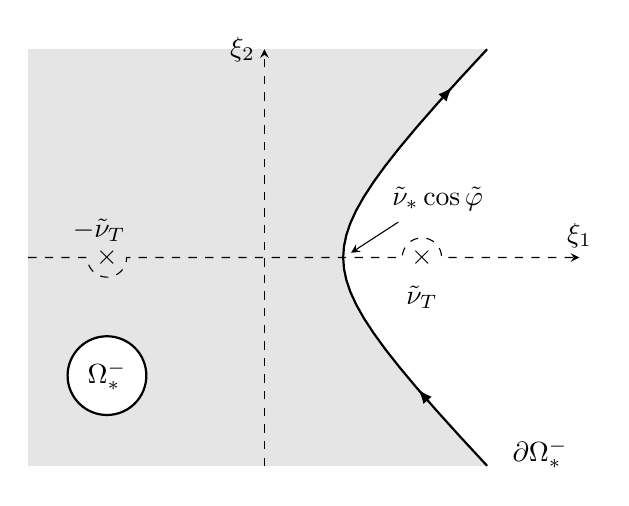
\begin{tikzpicture}
	% Filling Omega_*^-
	\fill [color=gray!20]
	(-3,{-sinh(1.7)})
	-- plot [domain= -1.7:1.7] ({cosh(\x)},{sinh(\x)})
	-- (-3,{sinh(1.7)});
	
%	\fill [color=gray!20]
%	({cosh(1.7)},{-sinh(1.7)})
%	-- plot [domain= 0:-3] ({\x},{-sinh(1.7)})
%	-- (-3,0)
%	-- cycle;
	
%	\fill[color=white] (-2,0) circle (0.25);
	
	\draw[dashed, ->,>=stealth] (-3,0)  -- (-2.25,0) arc(-180:0:0.25)--(1.75,0) arc (180:0:0.25)--(4,0) node[above]{$\xi_1$};
	\draw[dashed, ->,>=stealth](0,{-sinh(1.7)})--(0,{sinh(1.7)}) node[left]{$\xi_2$};
	\node at (2,0) { $\times$}; 
%	\node at (0,1.5) { $\times$}; 
	\node at (2,-0.5) {$\nuti_T$};
%	\node at (0.5,1.5) {$\nuti_L$};
	\node at (-2,0) { $\times$};
%	\node at (0,-1.5) { $\times$}; 
	\node at (-2.1,0.35) {$-\nuti_T$};
%	\node at (-0.5,-1.5) {$-\nuti_L$};
	
	% Hyperbola (contour  partial_Omega_0 )
	\draw[black, thick,decoration={ markings,  % This schema allows for fine-tuning the positions of arrows 
		mark=at position 0.2 with {\arrow{latex}},
		mark=at position 0.9 with {\arrow{latex}}},
	postaction={decorate}][domain=-1.7:1.7] plot({cosh(\x)}, {sinh(\x)});
	
	\node at (3.5,-2.5) {$\partial \Omega_*^-$};
	\draw[thin, ->,>=stealth](1.7,0.45) -- (1.1, 0.06);
	\node at (2.2, 0.75) { $\nuti_*\cos \tilde{\varphi}$};

	% Espace Omega_0
\fill [color=white] (-2,-1.5) circle (0.5);
\draw[thick] (-2,-1.5) circle (0.5);
\node at (-2,-1.5) {$\Omega_*^-$};
	\end{tikzpicture}
	\caption{Domain $\Omega_*^-$ and contour $\partial\Omega_*^-$ in the case $\noncr$.}
	\label{C4:Omegamoinsnoncr}
	\end{subfigure}
	\hfill
	\begin{subfigure}[b]{0.45\textwidth}
	    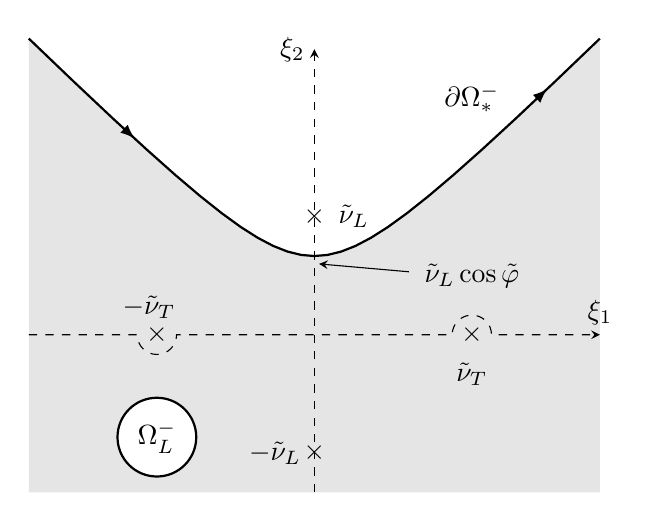
\begin{tikzpicture}
	    	% Filling Omega_*^-
	\fill [color=gray!20]
	({-sinh(2)},-2)
	-- plot [domain= -2:2] ({sinh(\x)},{cosh(\x)})
	--({sinh(2)},-2);

	\draw[dashed, ->,>=stealth] (-3.6269,0)  -- (-2.25,0) arc(-180:0:0.25)--(1.75,0) arc (180:0:0.25)--(3.6269,0) node[above]{$\xi_1$};
	
	\draw[dashed, ->,>=stealth](0,-2)--(0,{sinh(2)}) node[left]{$\xi_2$};
	\node at (2,0) { $\times$}; 
	\node at (0,1.5) { $\times$}; 
	\node at (2,-0.5) {$\nuti_T$};
	\node at (0.5,1.5) {$\nuti_L$};
	\node at (-2,0) { $\times$};
	\node at (0,-1.5) { $\times$}; 
	\node at (-2.1,0.35) {$-\nuti_T$};
	\node at (-0.5,-1.5) {$-\nuti_L$};
	
	% Hyperbola (contour  partial_Omega_0 )
	\draw[black, thick,decoration={ markings,
		mark=at position 0.2 with {\arrow{latex}},
		mark=at position 0.9 with {\arrow{latex}}},
	postaction={decorate}][domain=-2:2] plot({sinh(\x)},{cosh(\x)});
	
	\node at (2,3) {$\partial \Omega_*^-$};
	\draw[thin, ->,>=stealth](1.2,0.8) -- (0.06,0.9);
	\node at (2, 0.75) { $\nuti_L\cos \tilde{\varphi}$};

	% Espace Omega_0
\fill [color=white] (-2,-1.3) circle (0.5);
\draw[thick] (-2,-1.3) circle (0.5);
\node at (-2,-1.3) {$\Omega_L^-$};

	    \end{tikzpicture}
	    \label{C4:OmegamoinsL}
	    \caption{Domain $\Omega_L^-$ and contour $\partial\Omega_L^-$ in the case $\crit$.}
	\end{subfigure}
\caption{Domains $\Omega_*^-$ and contours $\partial \Omega_*^-$ in cases $\noncr$ and $\crit$.}
\label{C4:dOmegamoins}
\end{figure}

The recursive system of functional equations solved by the regular part is obtained by substituting \eqref{C4:DM2} and \eqref{C4:TM2} into \eqref{C4:regparteqn}:
\begin{equation}
\left\{
\begin{matrix}
X_1(\xi) =g_1(\xi)-\textbf{dm}^{-1}(\xi).\underset{*=L,T}{\sum} \mathbf{M}_*(\xi).X_2(T_*^{-1}(\xi))\textbf{1}_{\Omega_*^-}(\xi) \\
X_2(\xi) =g_2(\xi)-\textbf{dm}^{-1}(\xi).\underset{*=L,T}{\sum} \mathbf{M}_*(\xi).X_1(T_*^{-1}(\xi))\textbf{1}_{\Omega_*^-}(\xi)
\end{matrix}
\right.,
\label{C4:recur}
\end{equation}
where , for $j=1,2$
\begin{equation}
g_j(\xi)=\textbf{dm}^{-1}(\xi)\left( u_j(\xi)- \int_{\Gamma_2}  \textbf{DM}(\xi,\zeta)X_j(\zeta)\, d\zeta- \int_{\partial \Omega_*^-}  \textbf{TM}(\xi,\zeta)X_{3-j}(\zeta)\, d\zeta \right) 
\label{C4:g1g2}
\end{equation}
The same consideration as those made in \ref{C3:propag} lead to an expression of functions $g_j$ using operators $\mathbb{D}(\cdot,\cdot)$ and $\mathbb{T}(\cdot,\cdot)$ :
\begin{equation}
\textbf{dm}(\xi).g_j(\xi)=u_j(\xi)-\sum_{k=1}^{2N} \sqrt{\frac{a_k}{\pi}}\left( \mathbb{ND}(a_k,\xi).\tilde{X}_j^k+\mathbb{NT}(a_k,\xi).\tilde{X}_{3-j}^k \right) ,
\label{C4:gjfinal}
\end{equation}
where
\begin{equation}
\mathbb{ND}(a,b)=\frac{1}{2\pi}\mathbb{D}(a,b)-\frac{\textbf{dm}(b)}{a+b}
\label{C4:defND}
\end{equation}
and
\begin{equation}
\mathbb{NT}(a,b)=\frac{1}{2i\pi}\mathbb{T}(a,b)-\sum_{*=L,T}\frac{\mathbf{M}_*(b)}{T^{-1}_*(b)+a} .
\end{equation}

In system \eqref{C4:recur}, the value of the regular part of the spectral function in domain $\Omega_*^-$, visible Fig.~\ref{C4:dOmegamoins}, is expressed using its value in the domain $\xi \notin \Omega_*^-$, where the numerical approximation \eqref{C4:Xj} is valid. To do so, functions $g_j,\, j=1,2$ are evaluated using \eqref{C4:gjfinal}. The accuracy of the numerical evaluation in domain $\xi \notin \Omega_*^-$ is therefore propagated to domain $\Omega_*^-$. 

This concludes the semi-analytical computation of the spectral functions. The L, TH and TV diffraction coefficients can now be computed using \eqref{C4:Dbeta}. Numerical testing is presented in the following. 

\section{Numerical Tests}
The spectral functions are evaluated numerically using the semi-analytical scheme described in the previous sections. This is achieved by, first, computing the poles and residues of the spectral functions analytically using the recursive algorithm described in subsection \ref{C4:singpart}. Then, the regular parts of the spectral functions are approached numerically by solving \eqref{C4:regparteqn} thanks to the Galerkin collocation method described in subsection \ref{C4:regpart}. In the case where $\noncr$, the Galerkin parameters are set to:
\begin{equation}
a_k=1.001+0.05e^{k\frac{\log 10}{4}}-1, \hspace{3em} b_k=a_k-0.1i, \hspace{3em} 1\leq k\leq20
\end{equation}
And in the case where $\crit$, meaning for the case of an incident transversal wave with $|\delta_inc|>\delta_c$ (with $\delta_c \approx 33^o$ in steel), the Galerkin parameters are set to
\begin{equation}
\begin{matrix}
a_k=1.001+0.05e^{k\frac{\log 10}{4}}-1, & b_k=a_k-0.1i, & 1\leq k\leq10\\
a_k=-i\lbrack 1.001+0.05e^{(k-10)\frac{\log 10}{4}}-1\rbrack, & b_k=a_k+0.1, & 11\leq k\leq20
\end{matrix}
\end{equation}
when $\crit$.

Finally, the solution is rendered accurate in the entire complex domain by applying the recursive procedure called the propagation of the solution described in subsection \ref{C4:propag}.

Following these steps, the diffraction coefficients have been computed using \eqref{C4:Dbeta} and tested numerically.

\subsection{Comparison to the 2D code}
The first test on the 3D code is to check that when $\delta_{\alpha}=0$, the results obtained using the 3D code are the same as those obtained using the 2D code presented in the previous chapter and which has been validated numerically and experimentally (see sections \ref{C3:numval} and \ref{C3:expval}). This has been checked for the theoretical computations and must also be verified numerically.

The spectral functions are evaluated at $\xi=\nuti_L\cos\theta -i10^{-8}$ (a small negative imaginary part is added to ensure that the recursive equations \eqref{C4:recur} are valid) every $0,5^o$ for $0\leq\theta\leq \varphi$ and for $\delta_{\alpha} =0^o$,  using the 3D code. The L and TH diffraction coefficients are computed using \eqref{C4:Dbeta}, for an elastic wave propagating in a steel wedge ($c_L=5700m.s^{-1}, \, \, c_T=3200m.s^{-1}$). For the 3D problem, TH waves defined by \eqref{C4:ivec} correspond to 2D T waves. The results are compared to the diffraction coefficients obtained using the 2D elastic code presented in the previous chapter.

\begin{figure}
\centering
    \begin{subfigure}[b]{0.44\textwidth}
        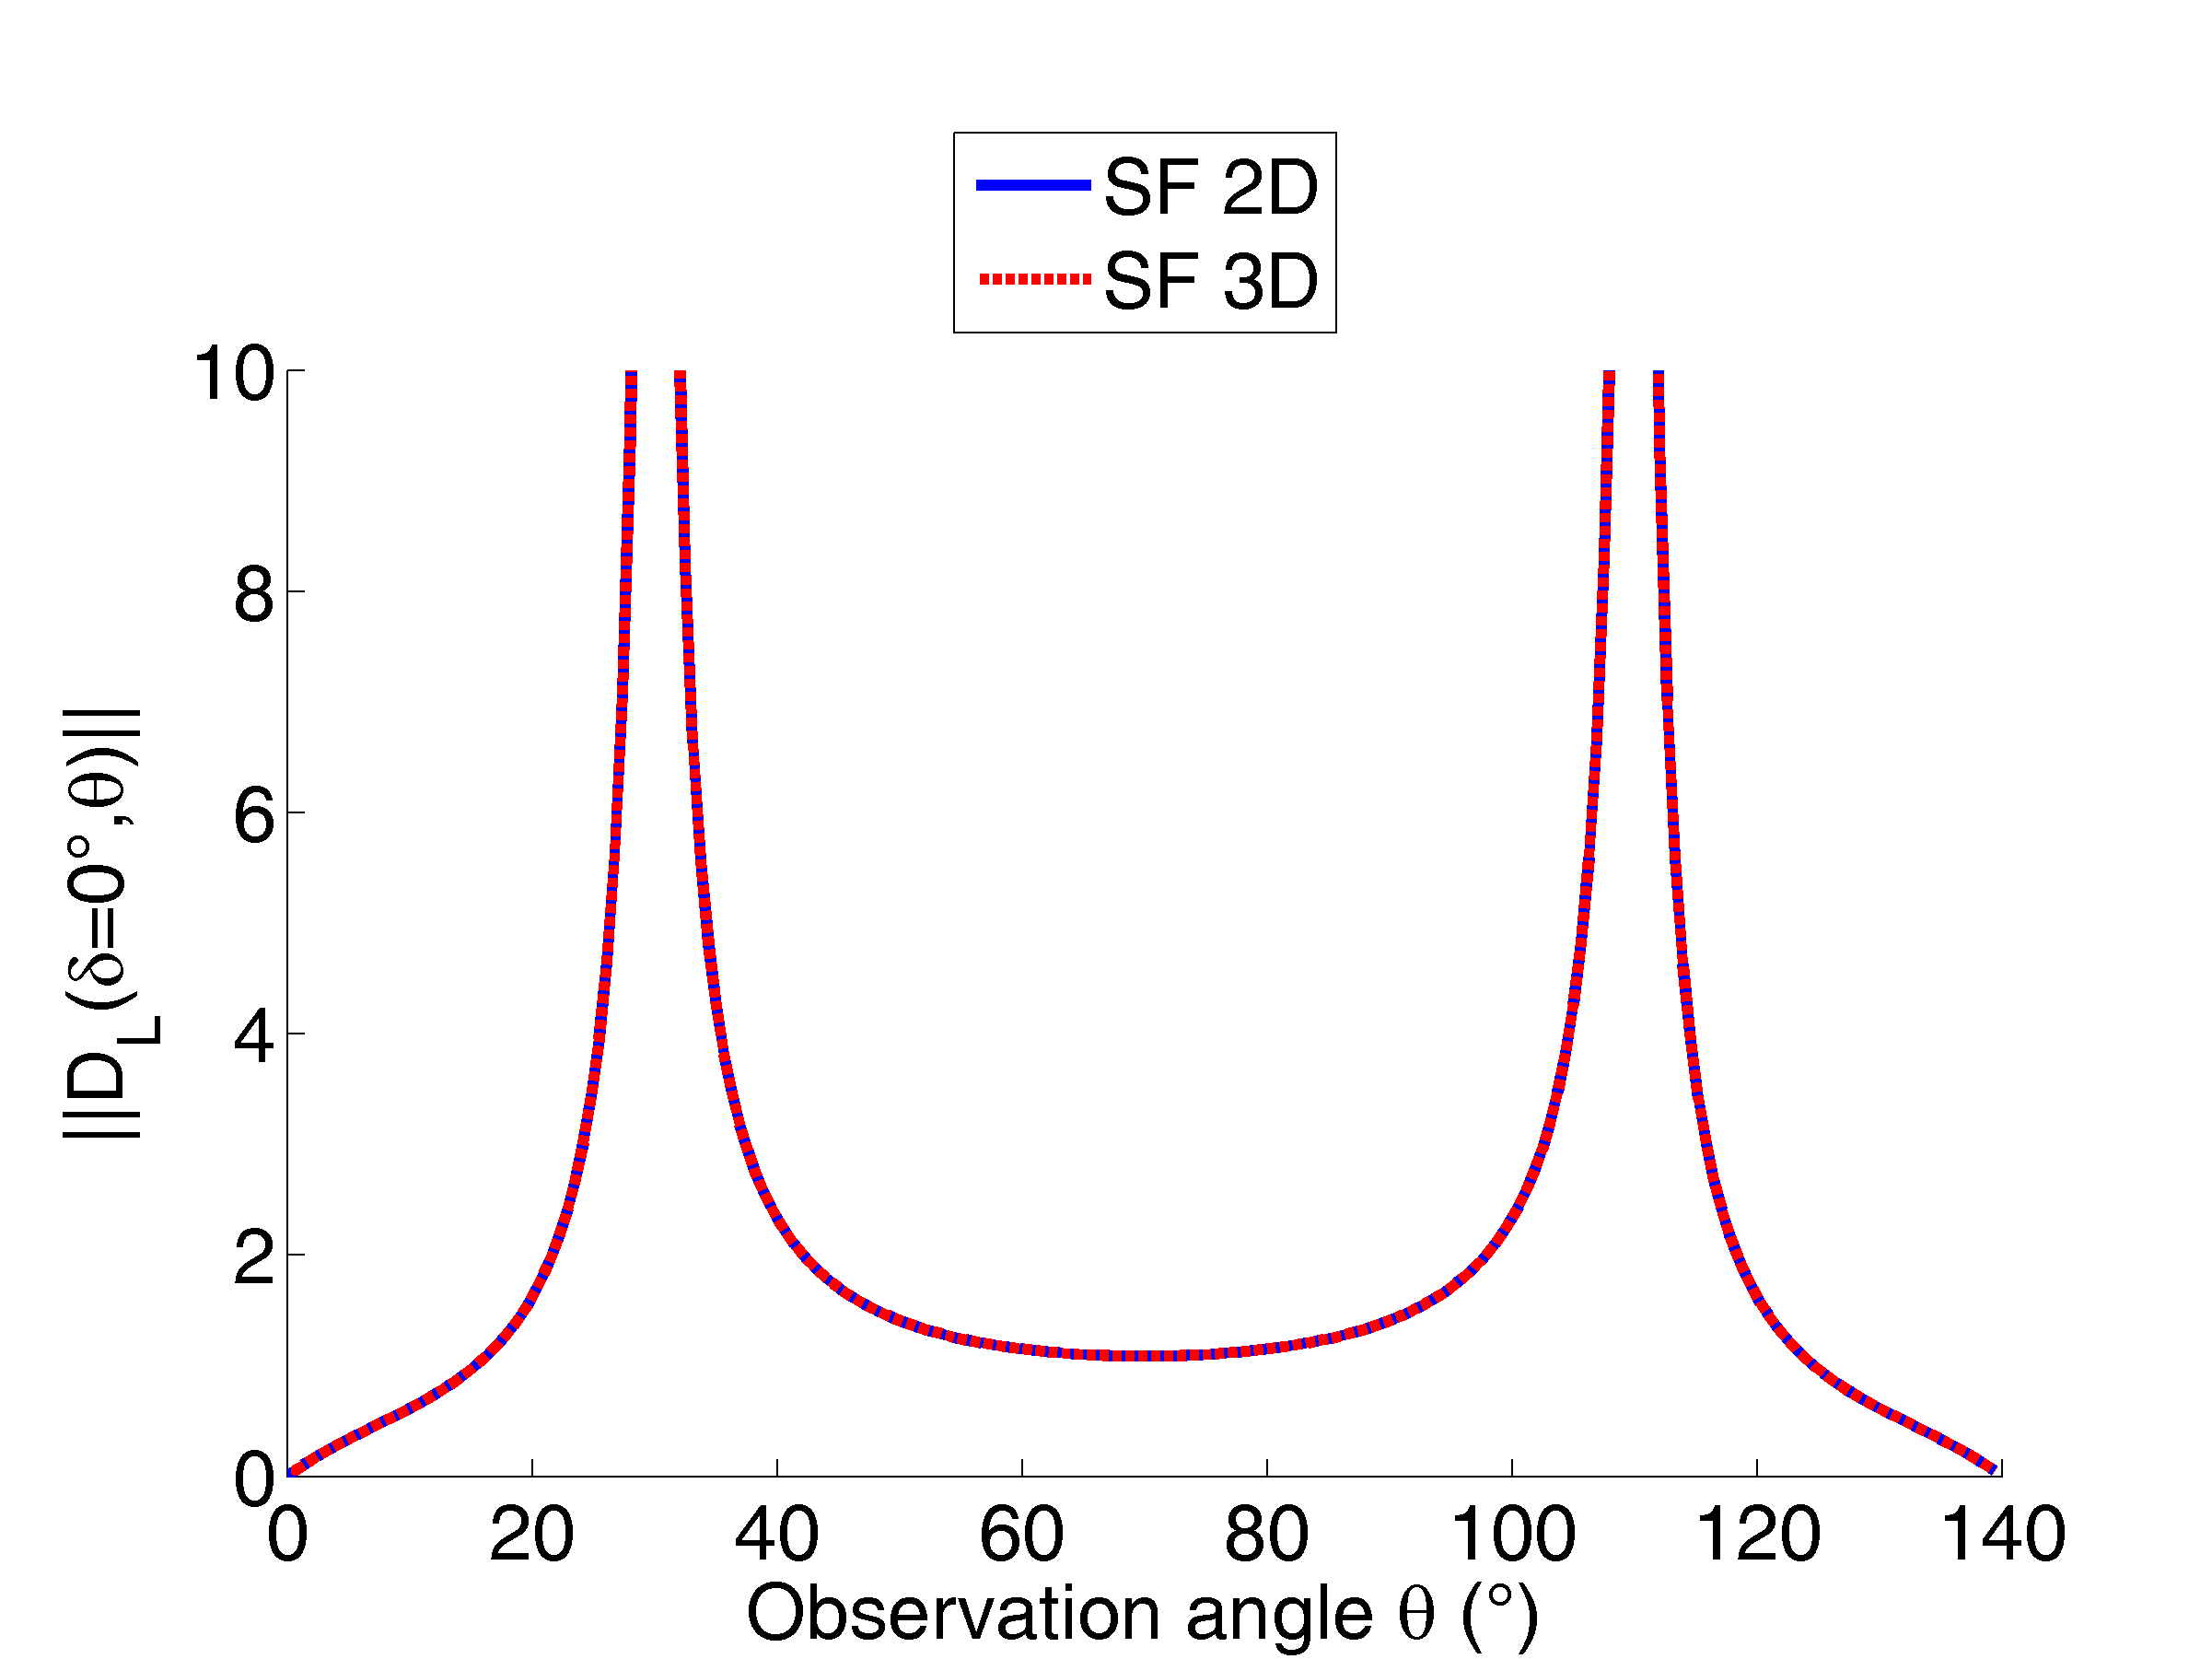
\includegraphics[width=\textwidth]{images/chapter4/XpropL_140_70_0_L.png}
        \caption{Diffracted and incident L waves.}
        \label{C4:DLL_14070}
    \end{subfigure}  
    \begin{subfigure}[b]{0.44\textwidth}
        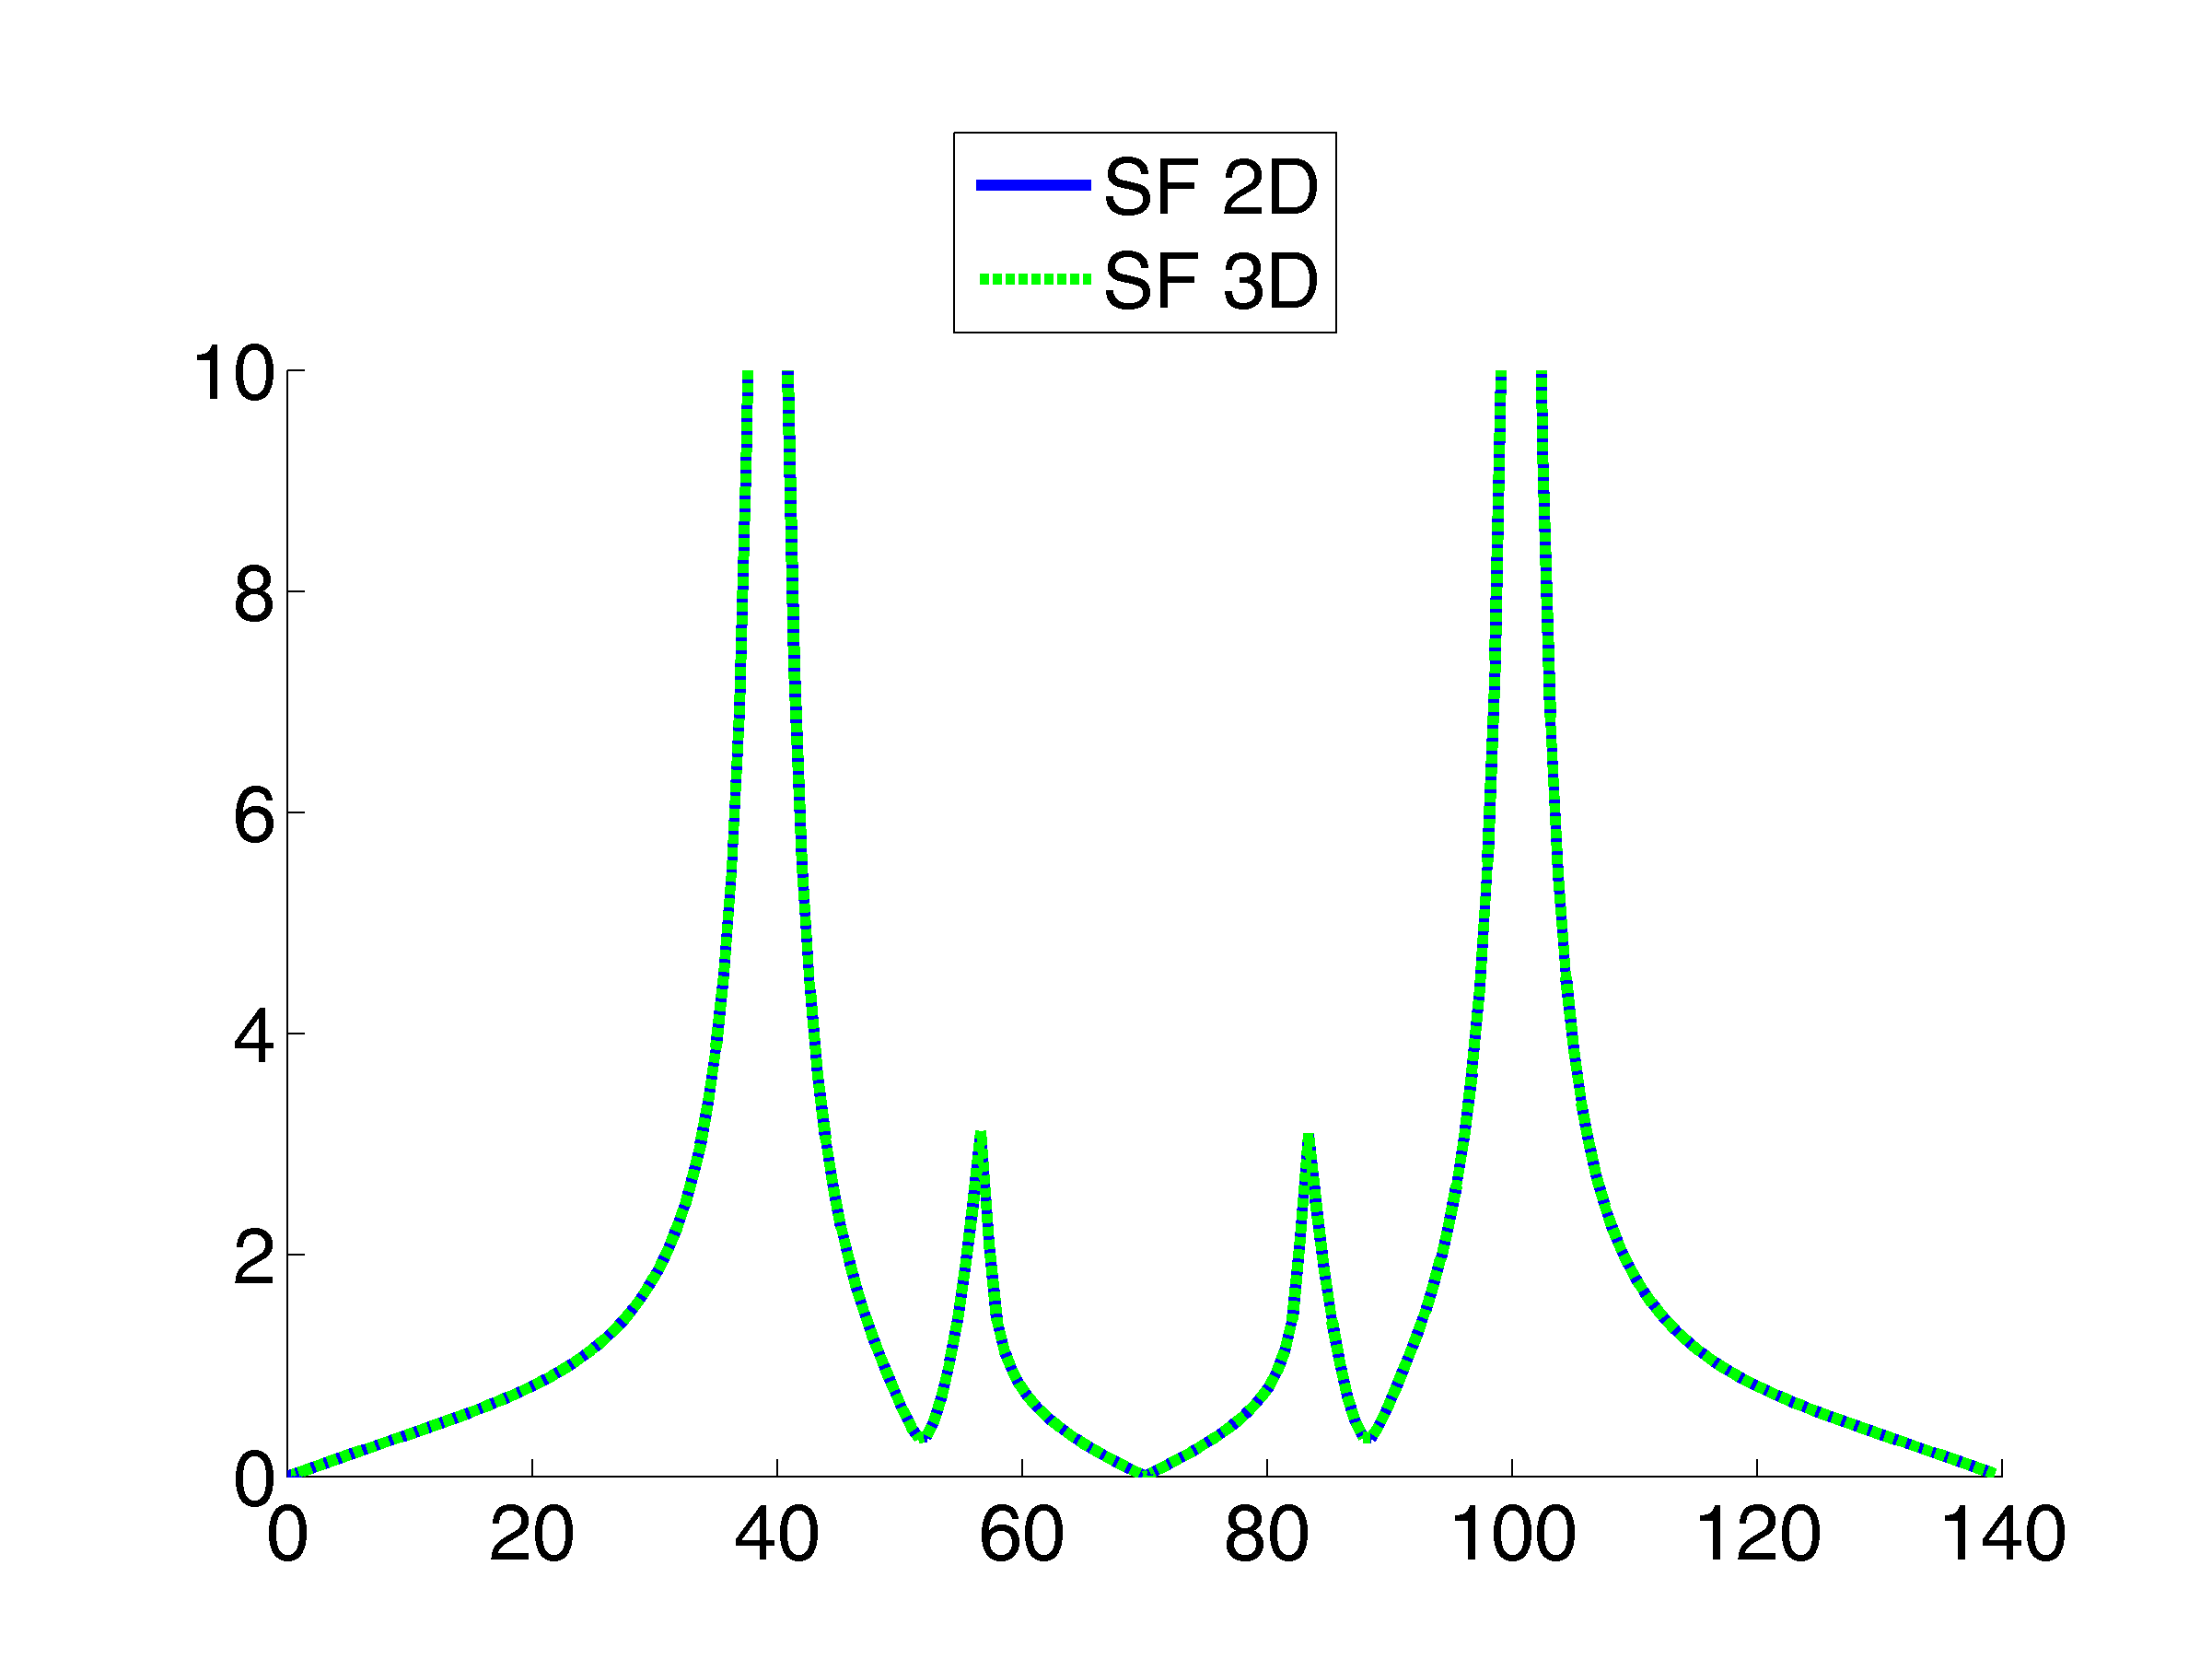
\includegraphics[width=\textwidth]{images/chapter4/XpropTH_140_70_0_L.png}
        \caption{Diffracted T wave and incident L wave.}
        \label{C4:DLT_14070}
     \end{subfigure}   
     \begin{subfigure}[b]{0.44\textwidth}
        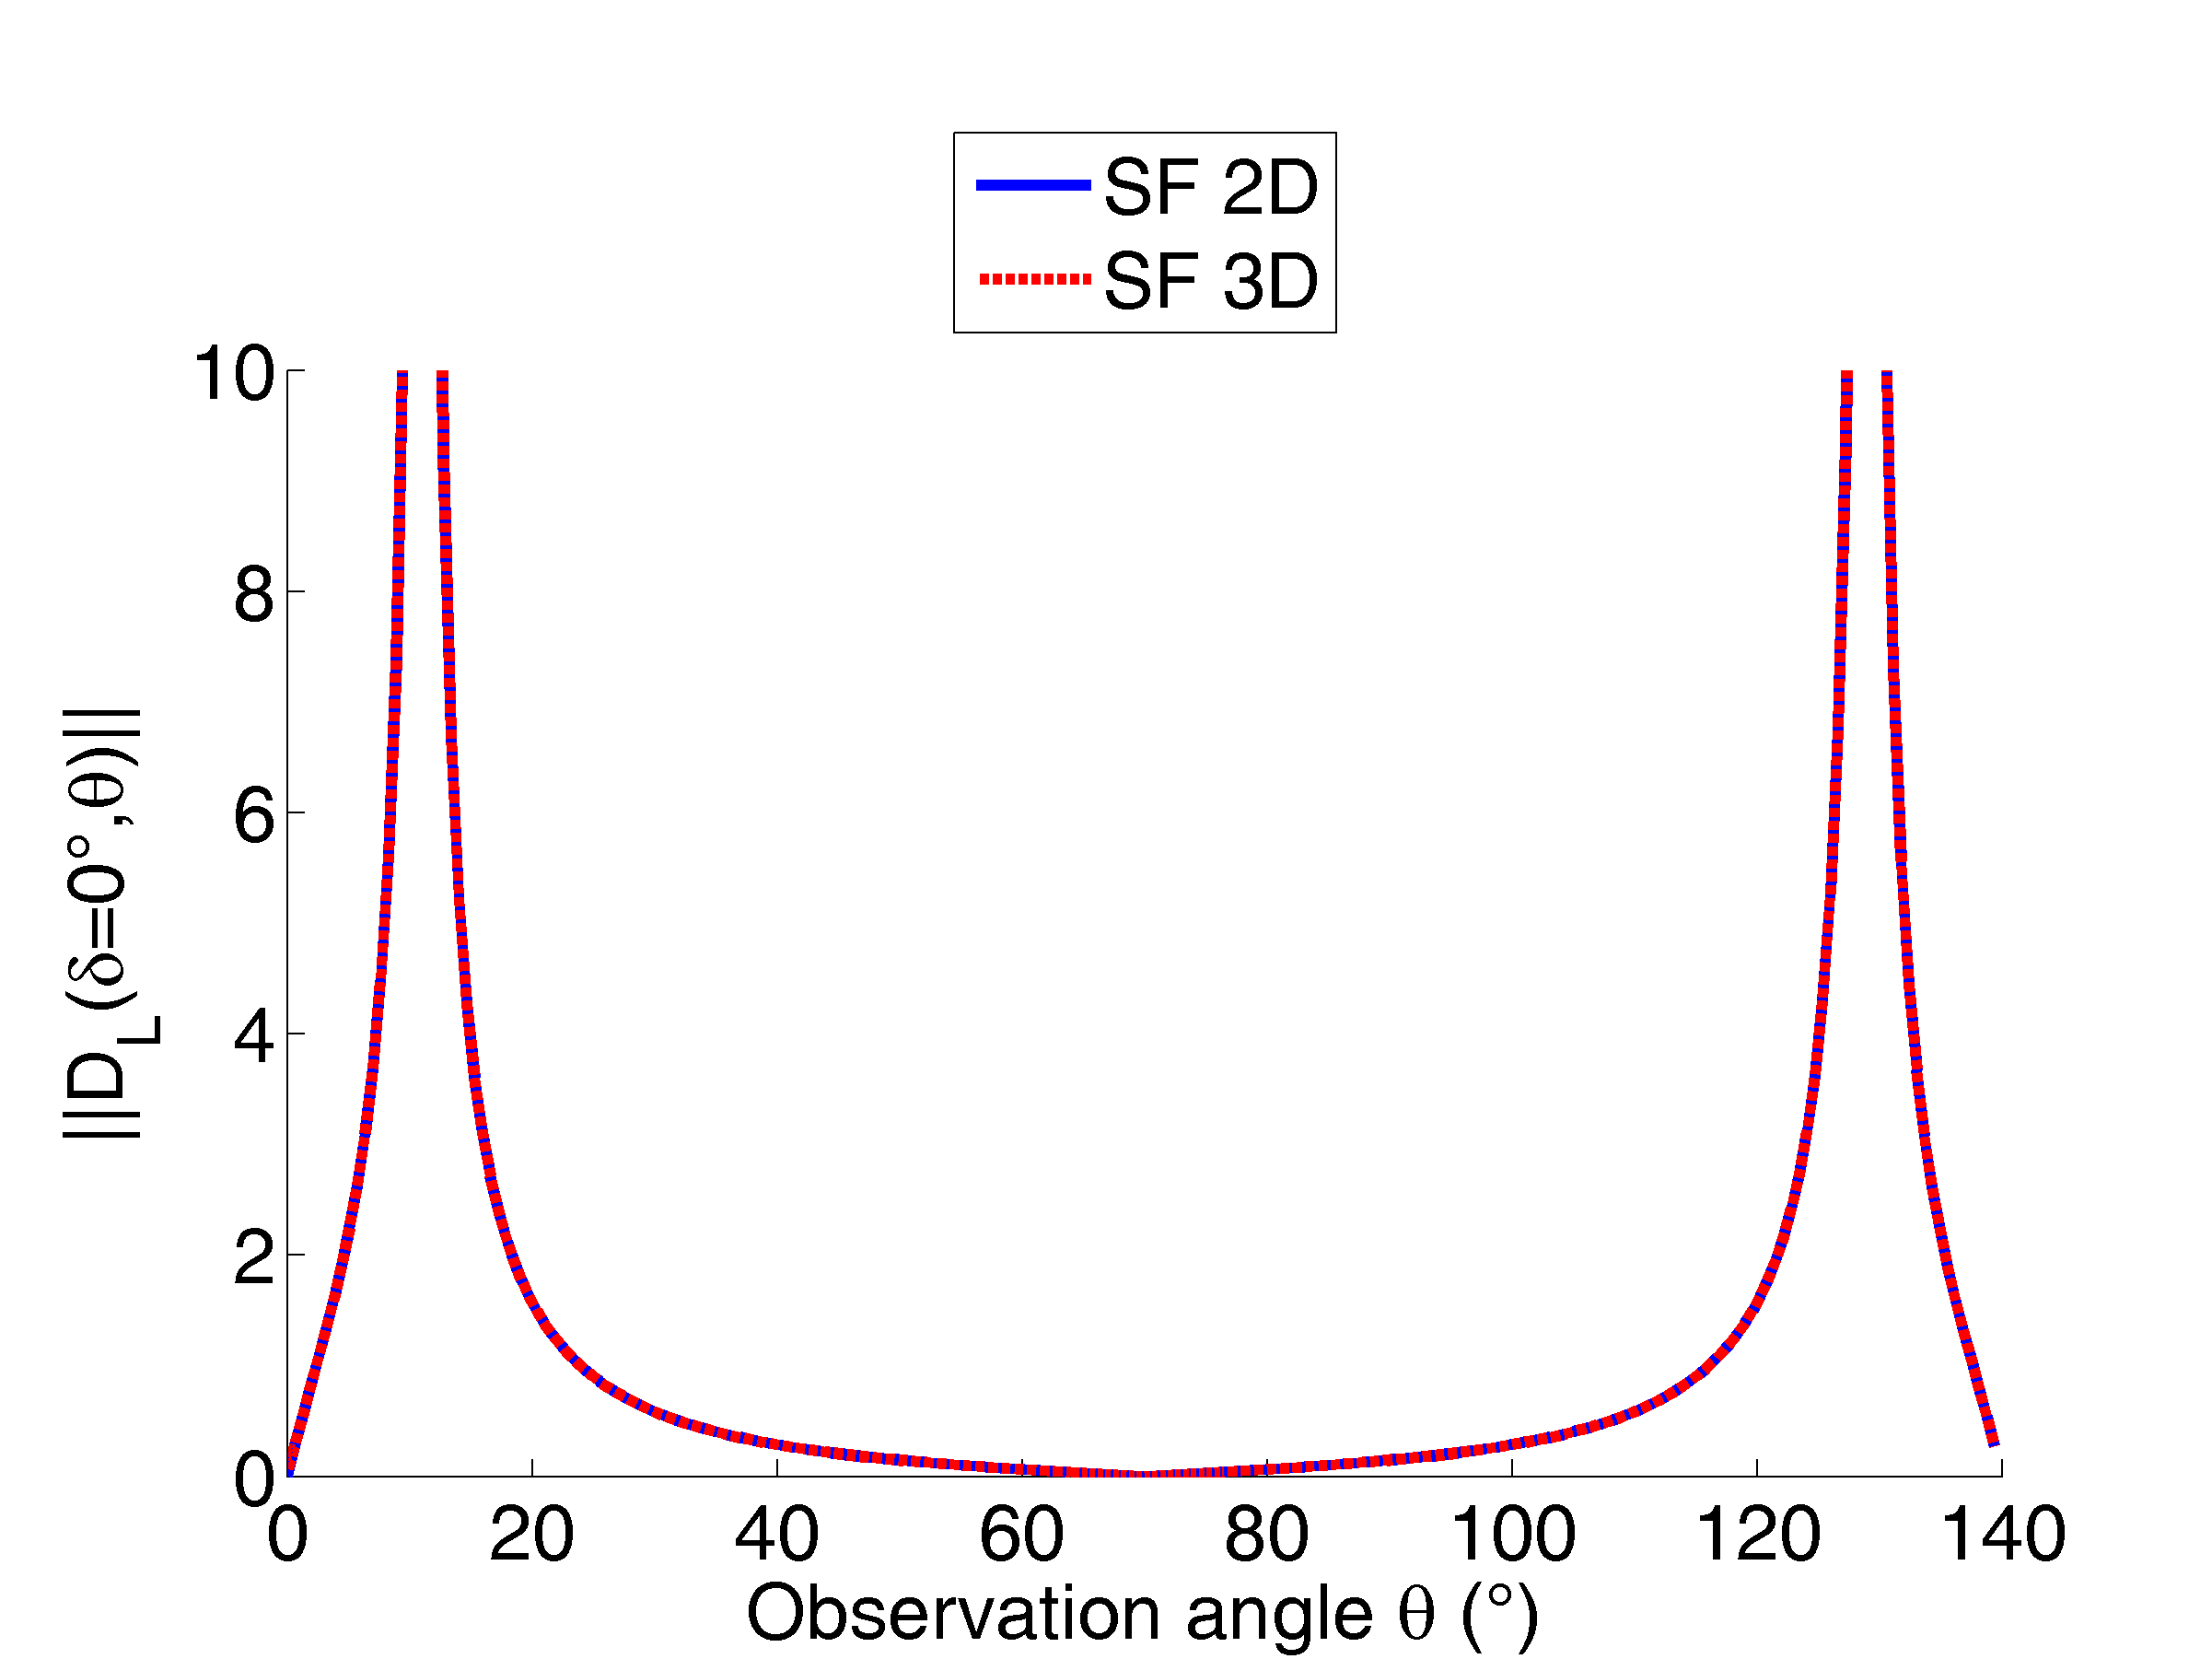
\includegraphics[width=\textwidth]{images/chapter4/XpropL_140_70_0_TH.png}
        \caption{Diffracted L wave and incident T wave.}
        \label{C4:DTL_14070}
    \end{subfigure}
    \begin{subfigure}[b]{0.44\textwidth}
        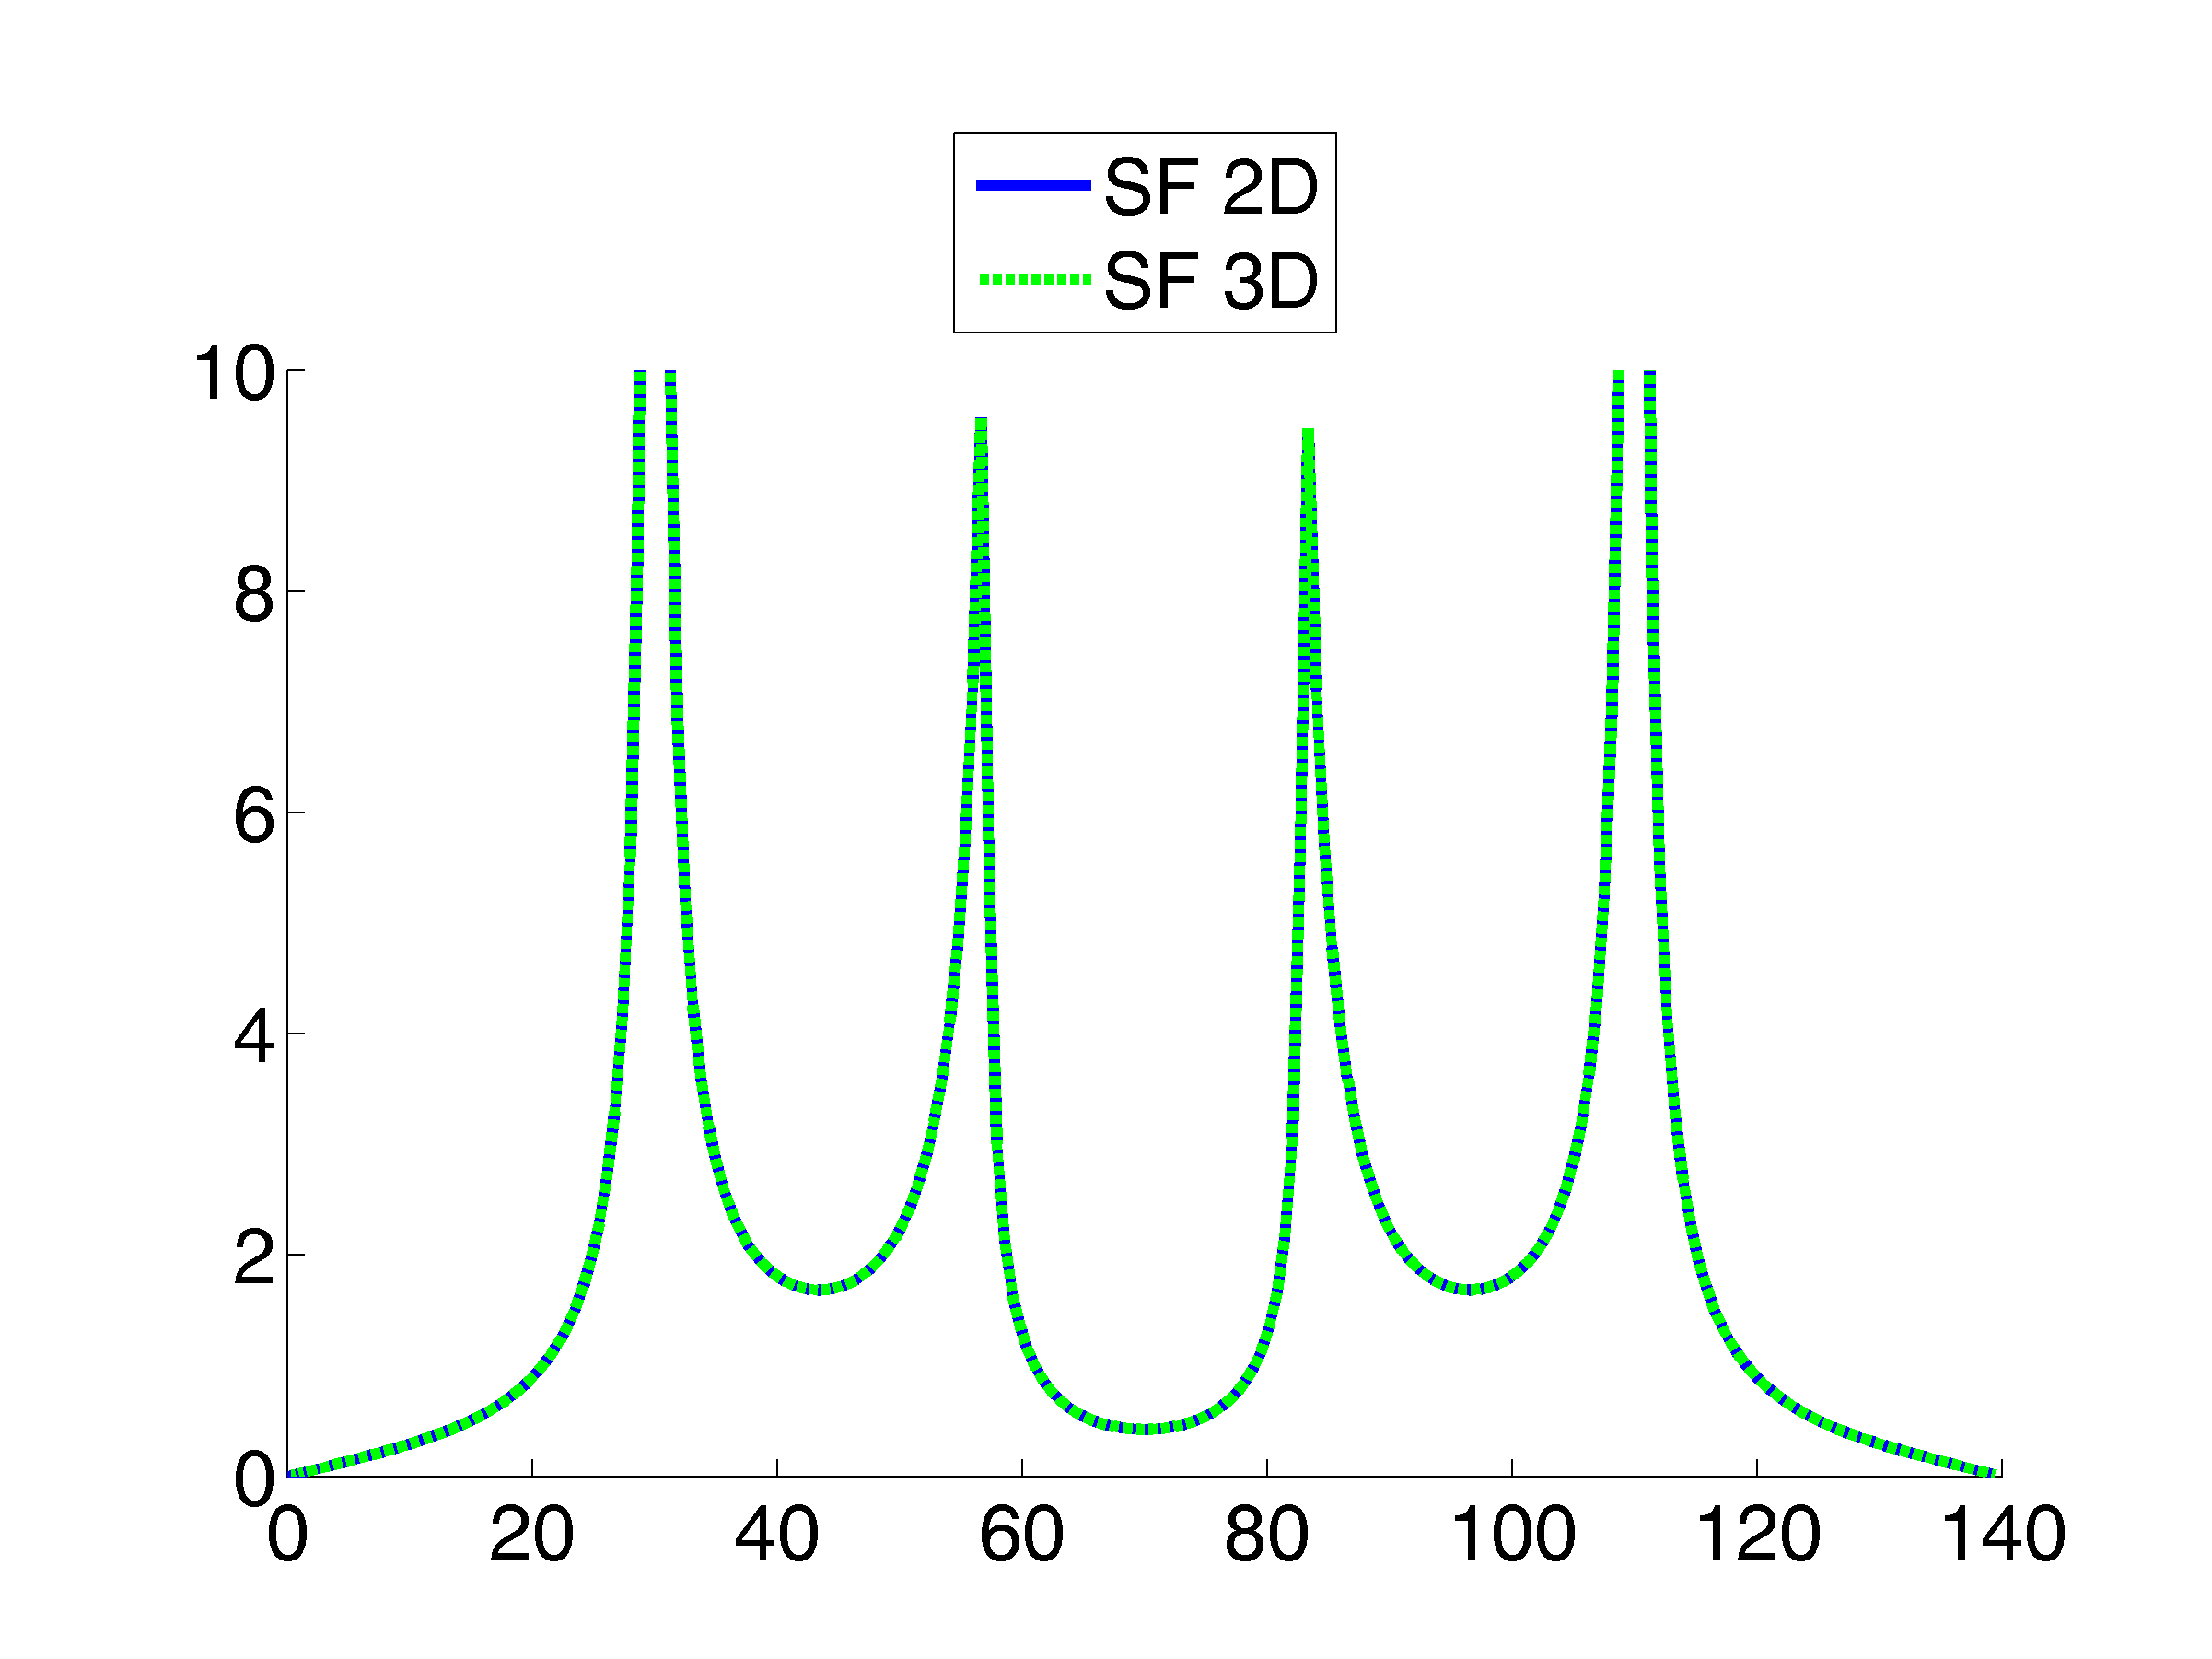
\includegraphics[width=\textwidth]{images/chapter4/XpropTH_140_70_0_TH.png}
        \caption{Diffracted and incident T waves.}
        \label{C4:DTT_14070}
     \end{subfigure}
     \caption{Diffraction coefficients for $\varphi=140^o, \theta_{inc}=70^o$}
     \label{C4:14070}
\end{figure}

Fig.~\ref{C4:14070} shows the absolute value of the diffraction coefficients obtained using the 2D and 3D \acrshort{sf} codes for a wedge of angle $\varphi=140^o$ illuminated by a wave incident with an angle $\theta_{inc}=70^o$. In Figs.~\ref{C4:DLL_14070} and \ref{C4:DTL_14070}, representing L diffraction coefficients, the thick blue line represents the results obtained using the 2D code and the dashed red line represents the results obtained using the 3D code. In Figs.~\ref{C4:DLT_14070} and \ref{C4:DTT_14070}, representing T diffraction coefficients, the thick blue line represents the results obtained using the 2D code and the dashed green line represents results obtained using the 3D code.

\begin{figure}
\centering
    \begin{subfigure}[b]{0.44\textwidth}
        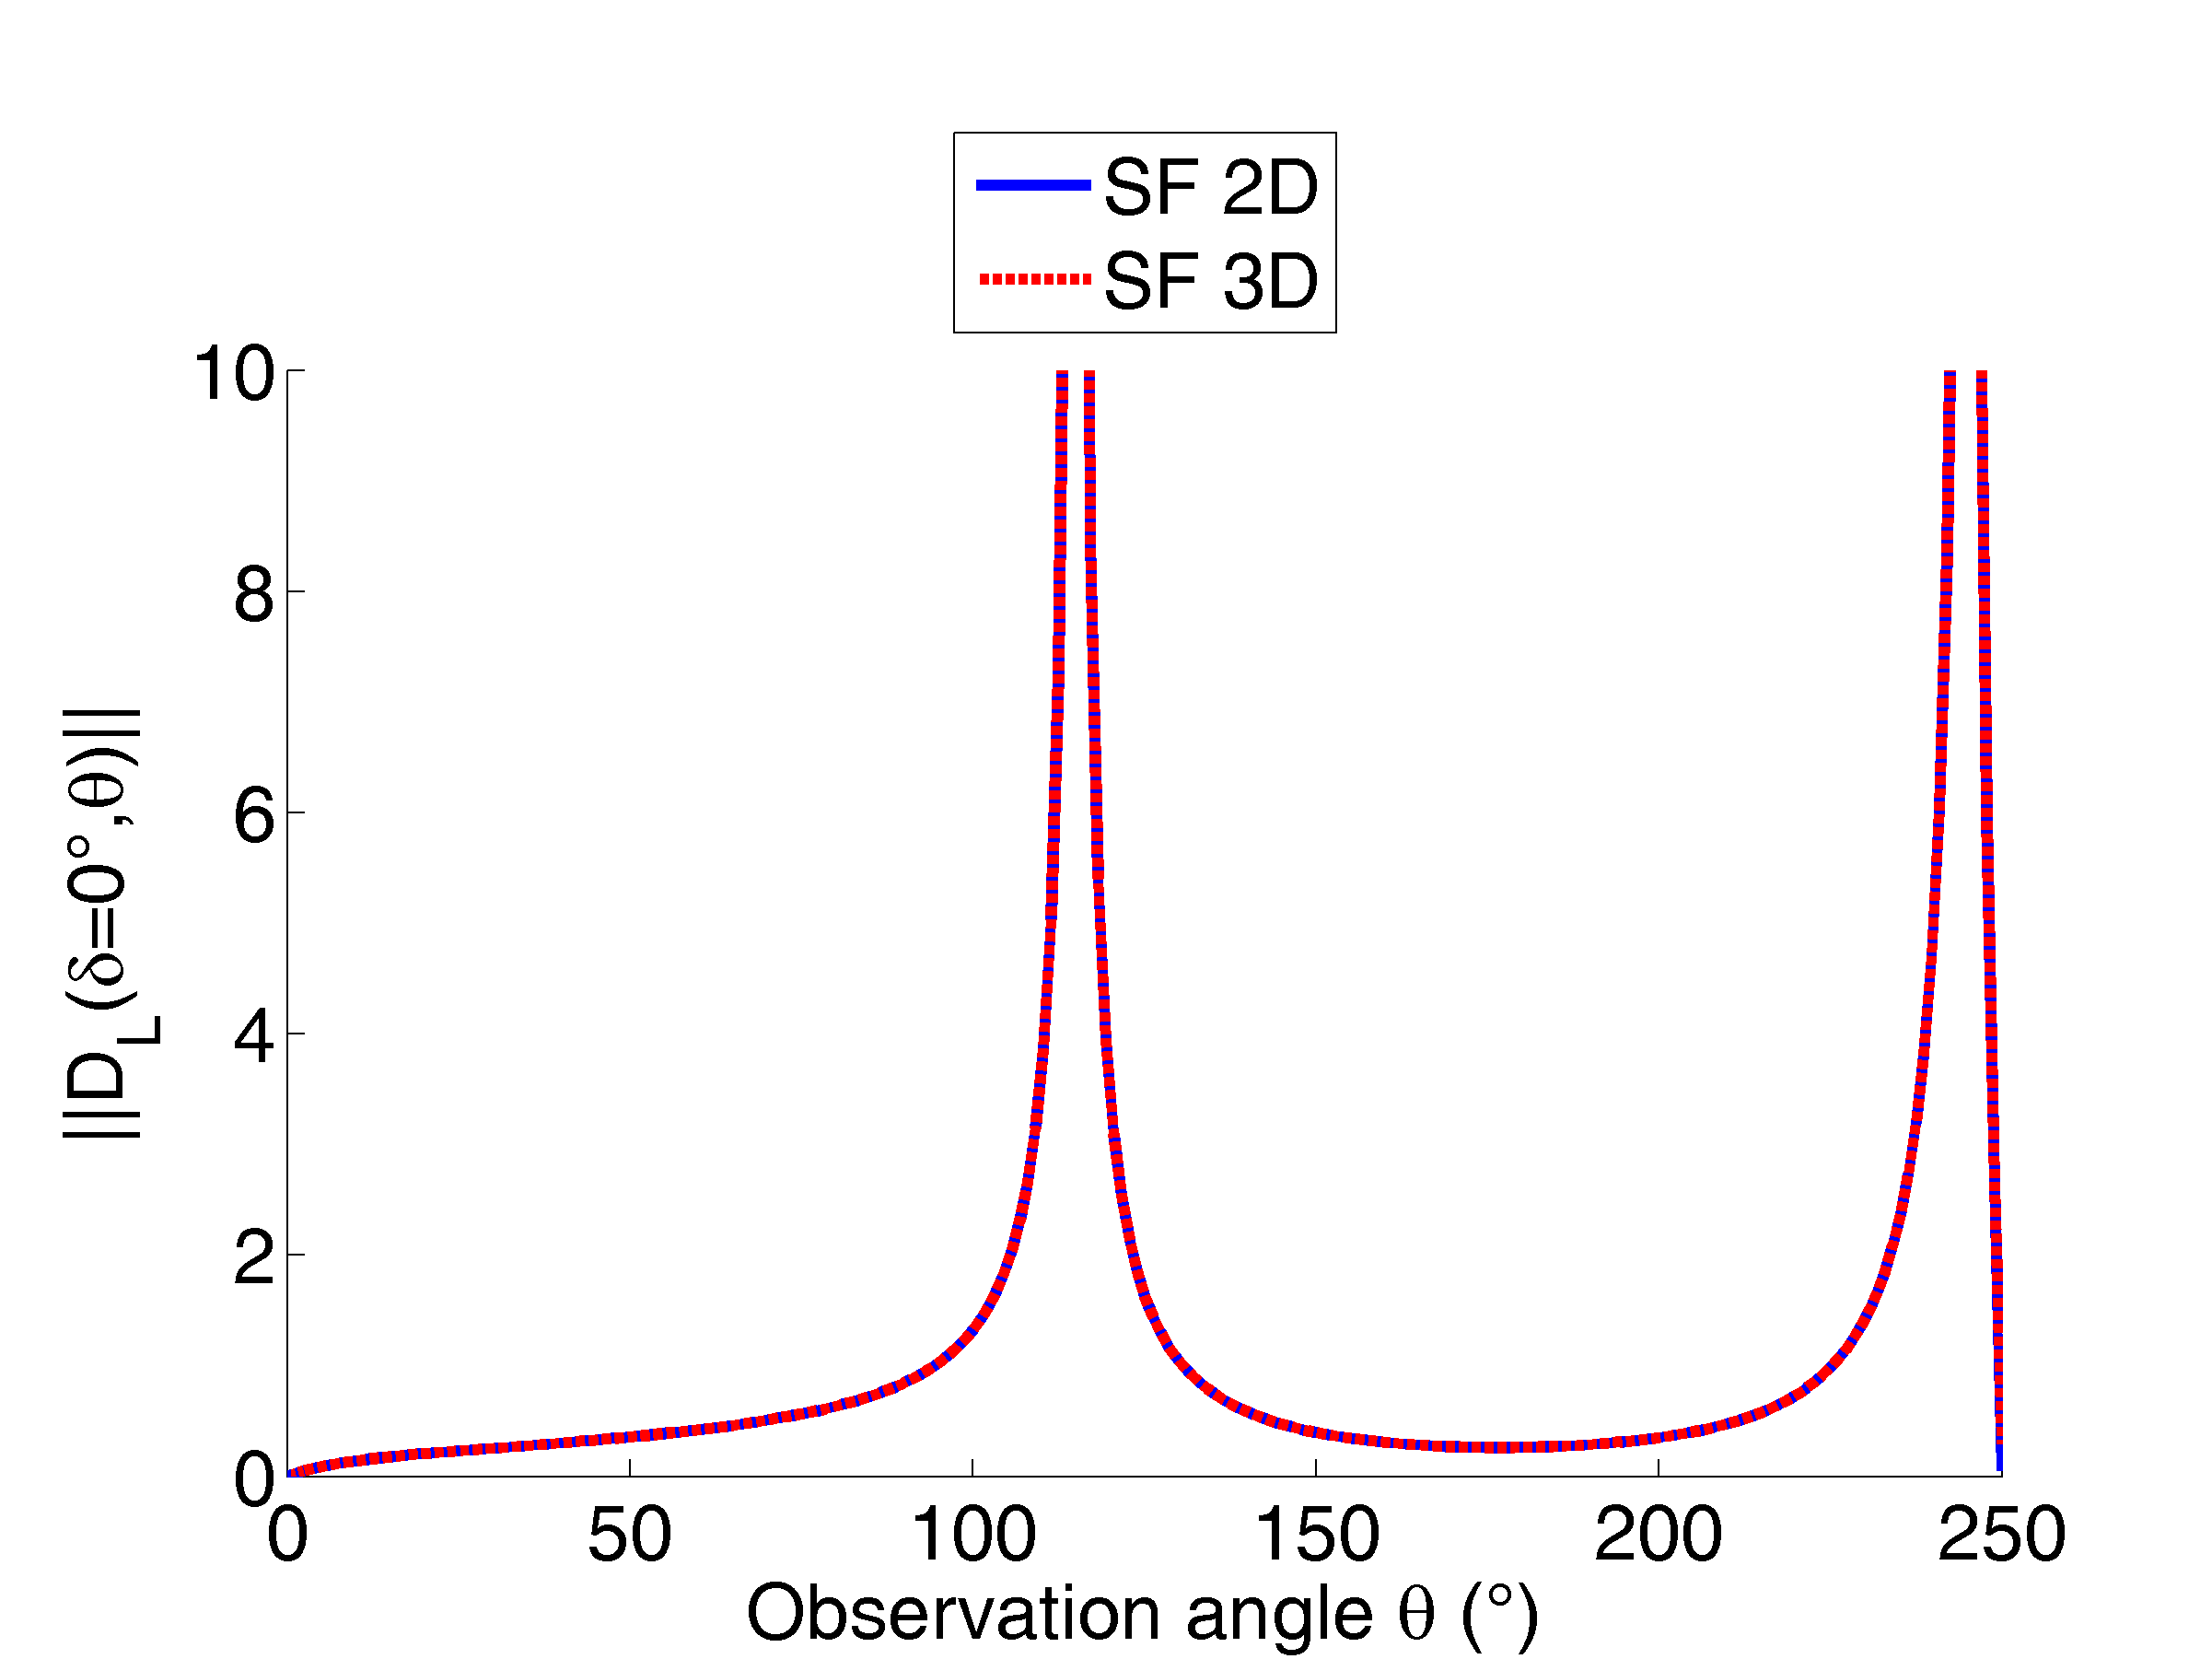
\includegraphics[width=\textwidth]{images/chapter4/XpropL_250_65_0_L.png}
        \caption{Diffracted and incident L waves.}
        \label{C4:DLL_25065}
    \end{subfigure}  
    \begin{subfigure}[b]{0.44\textwidth}
        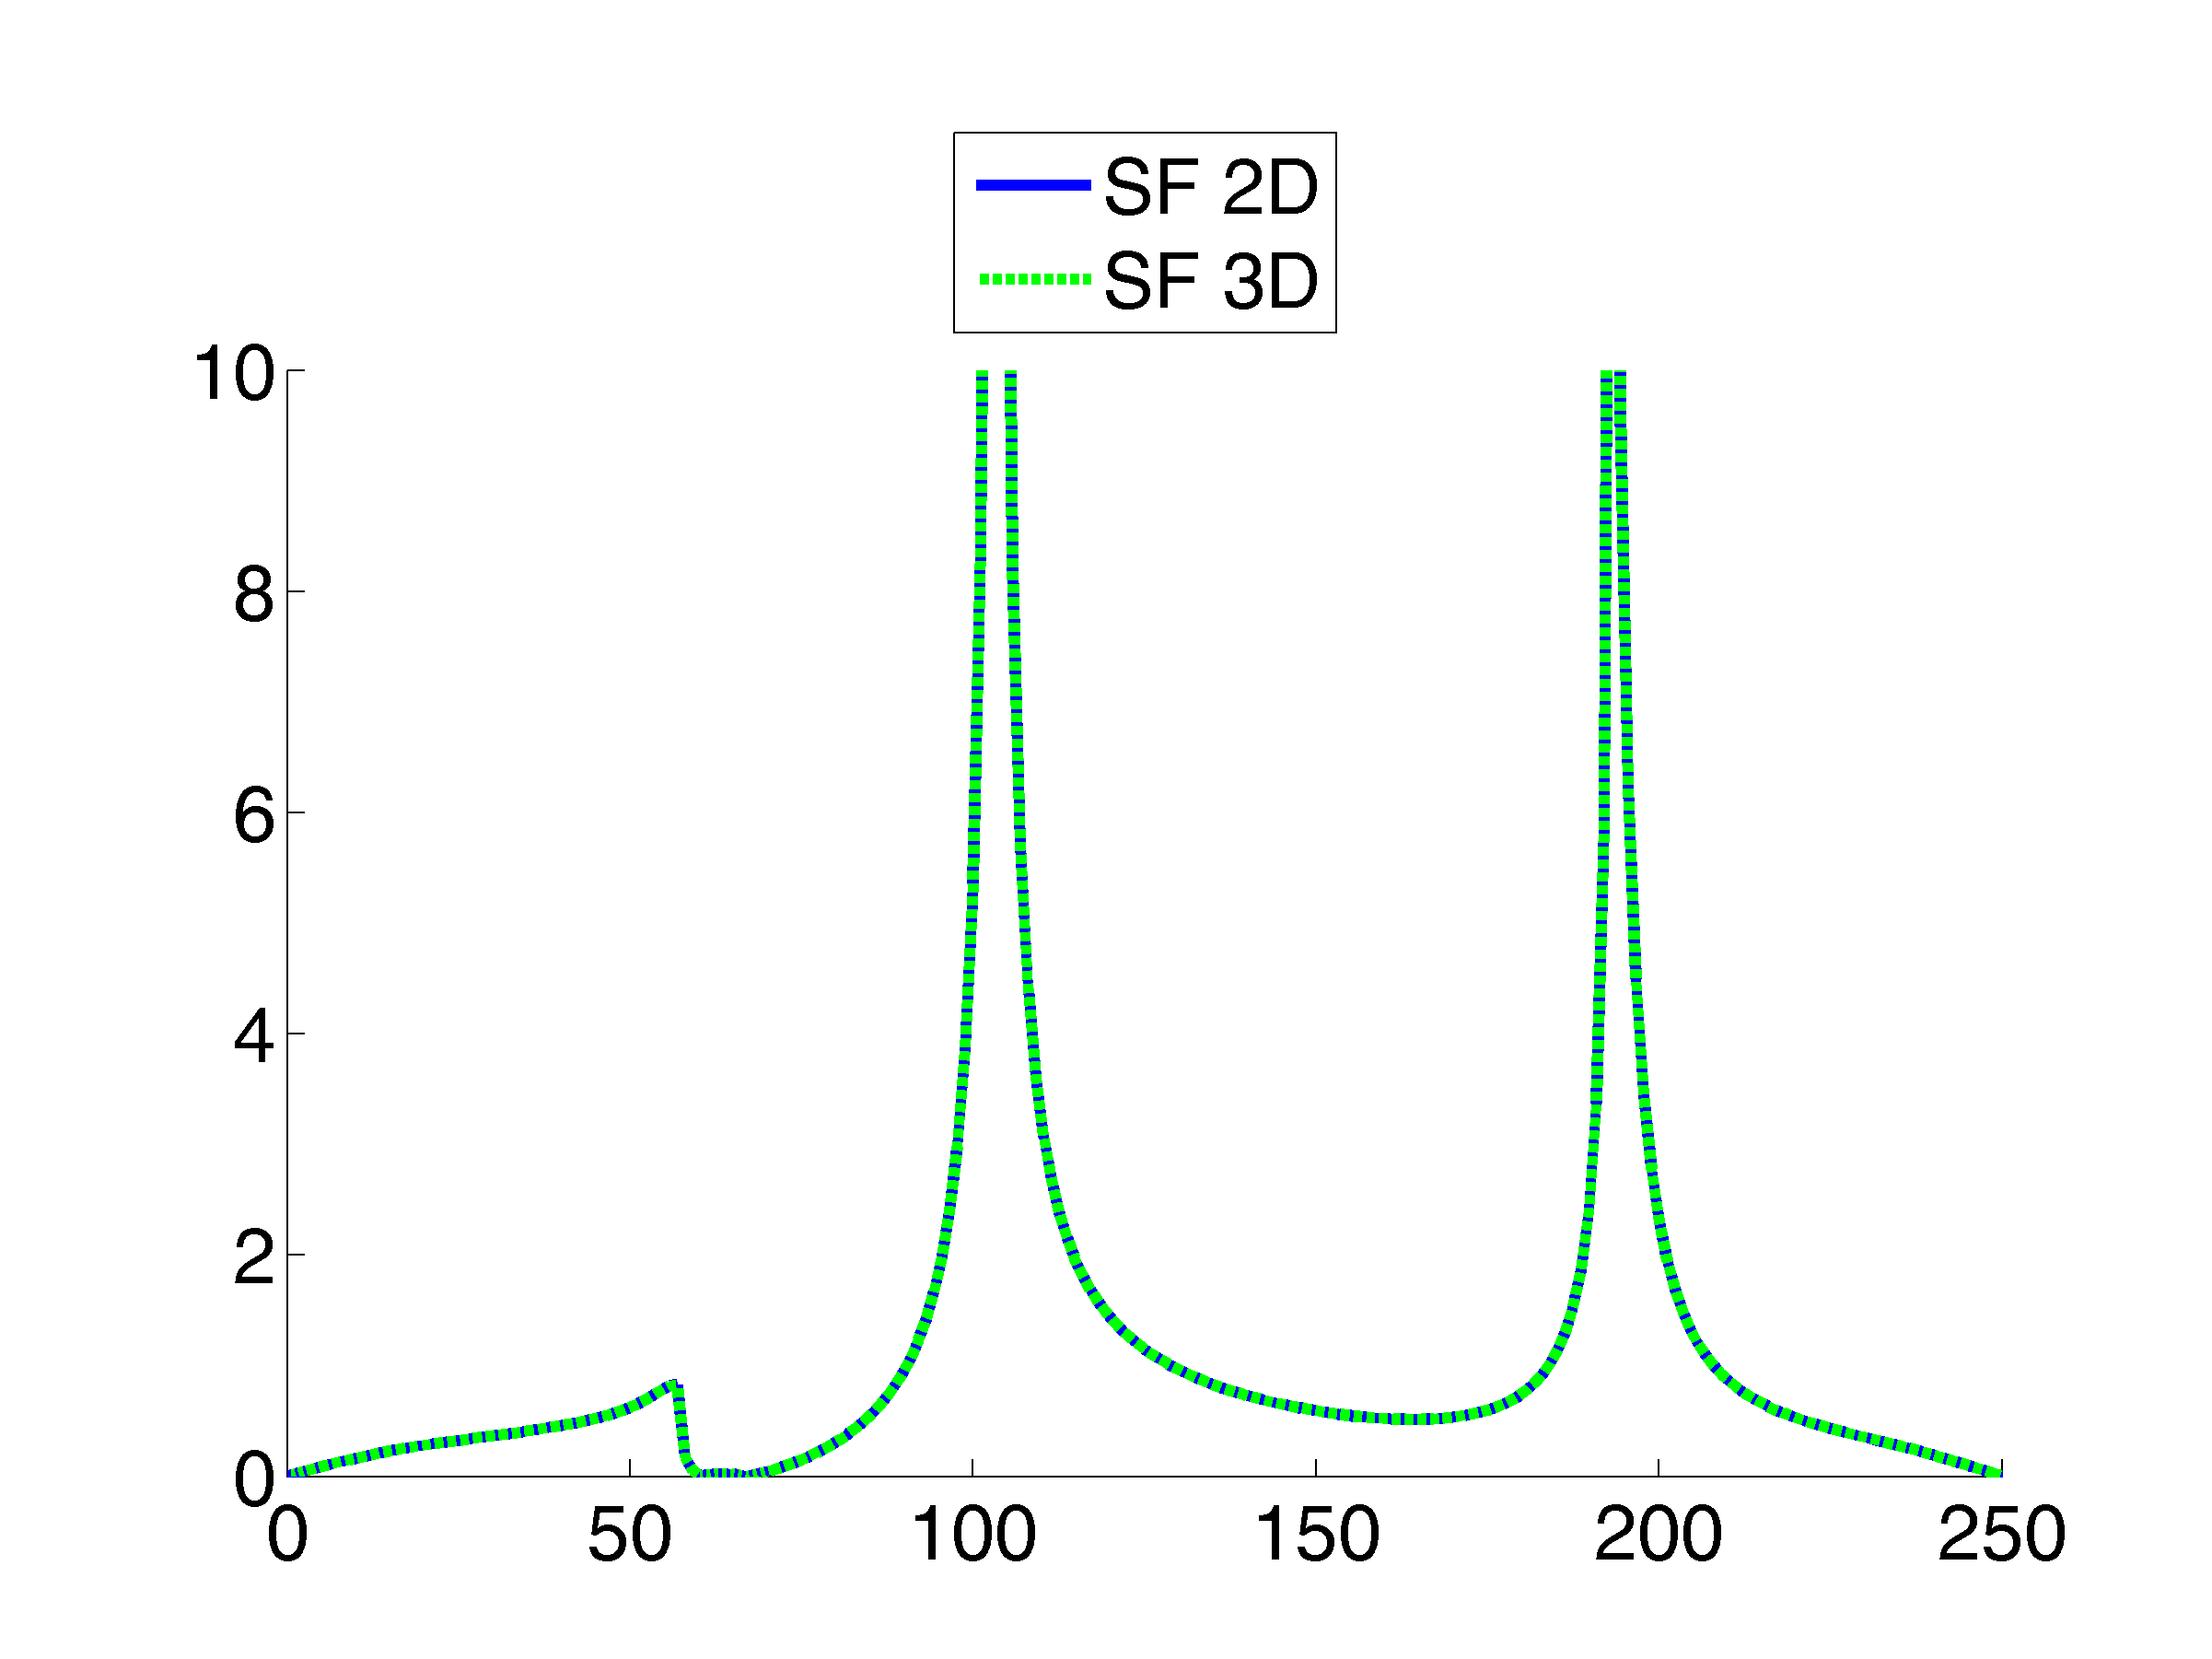
\includegraphics[width=\textwidth]{images/chapter4/XpropTH_250_65_0_L.png}
        \caption{Diffracted T wave and incident L wave.}
        \label{C4:DLT_25065}
     \end{subfigure}   
     \begin{subfigure}[b]{0.44\textwidth}
        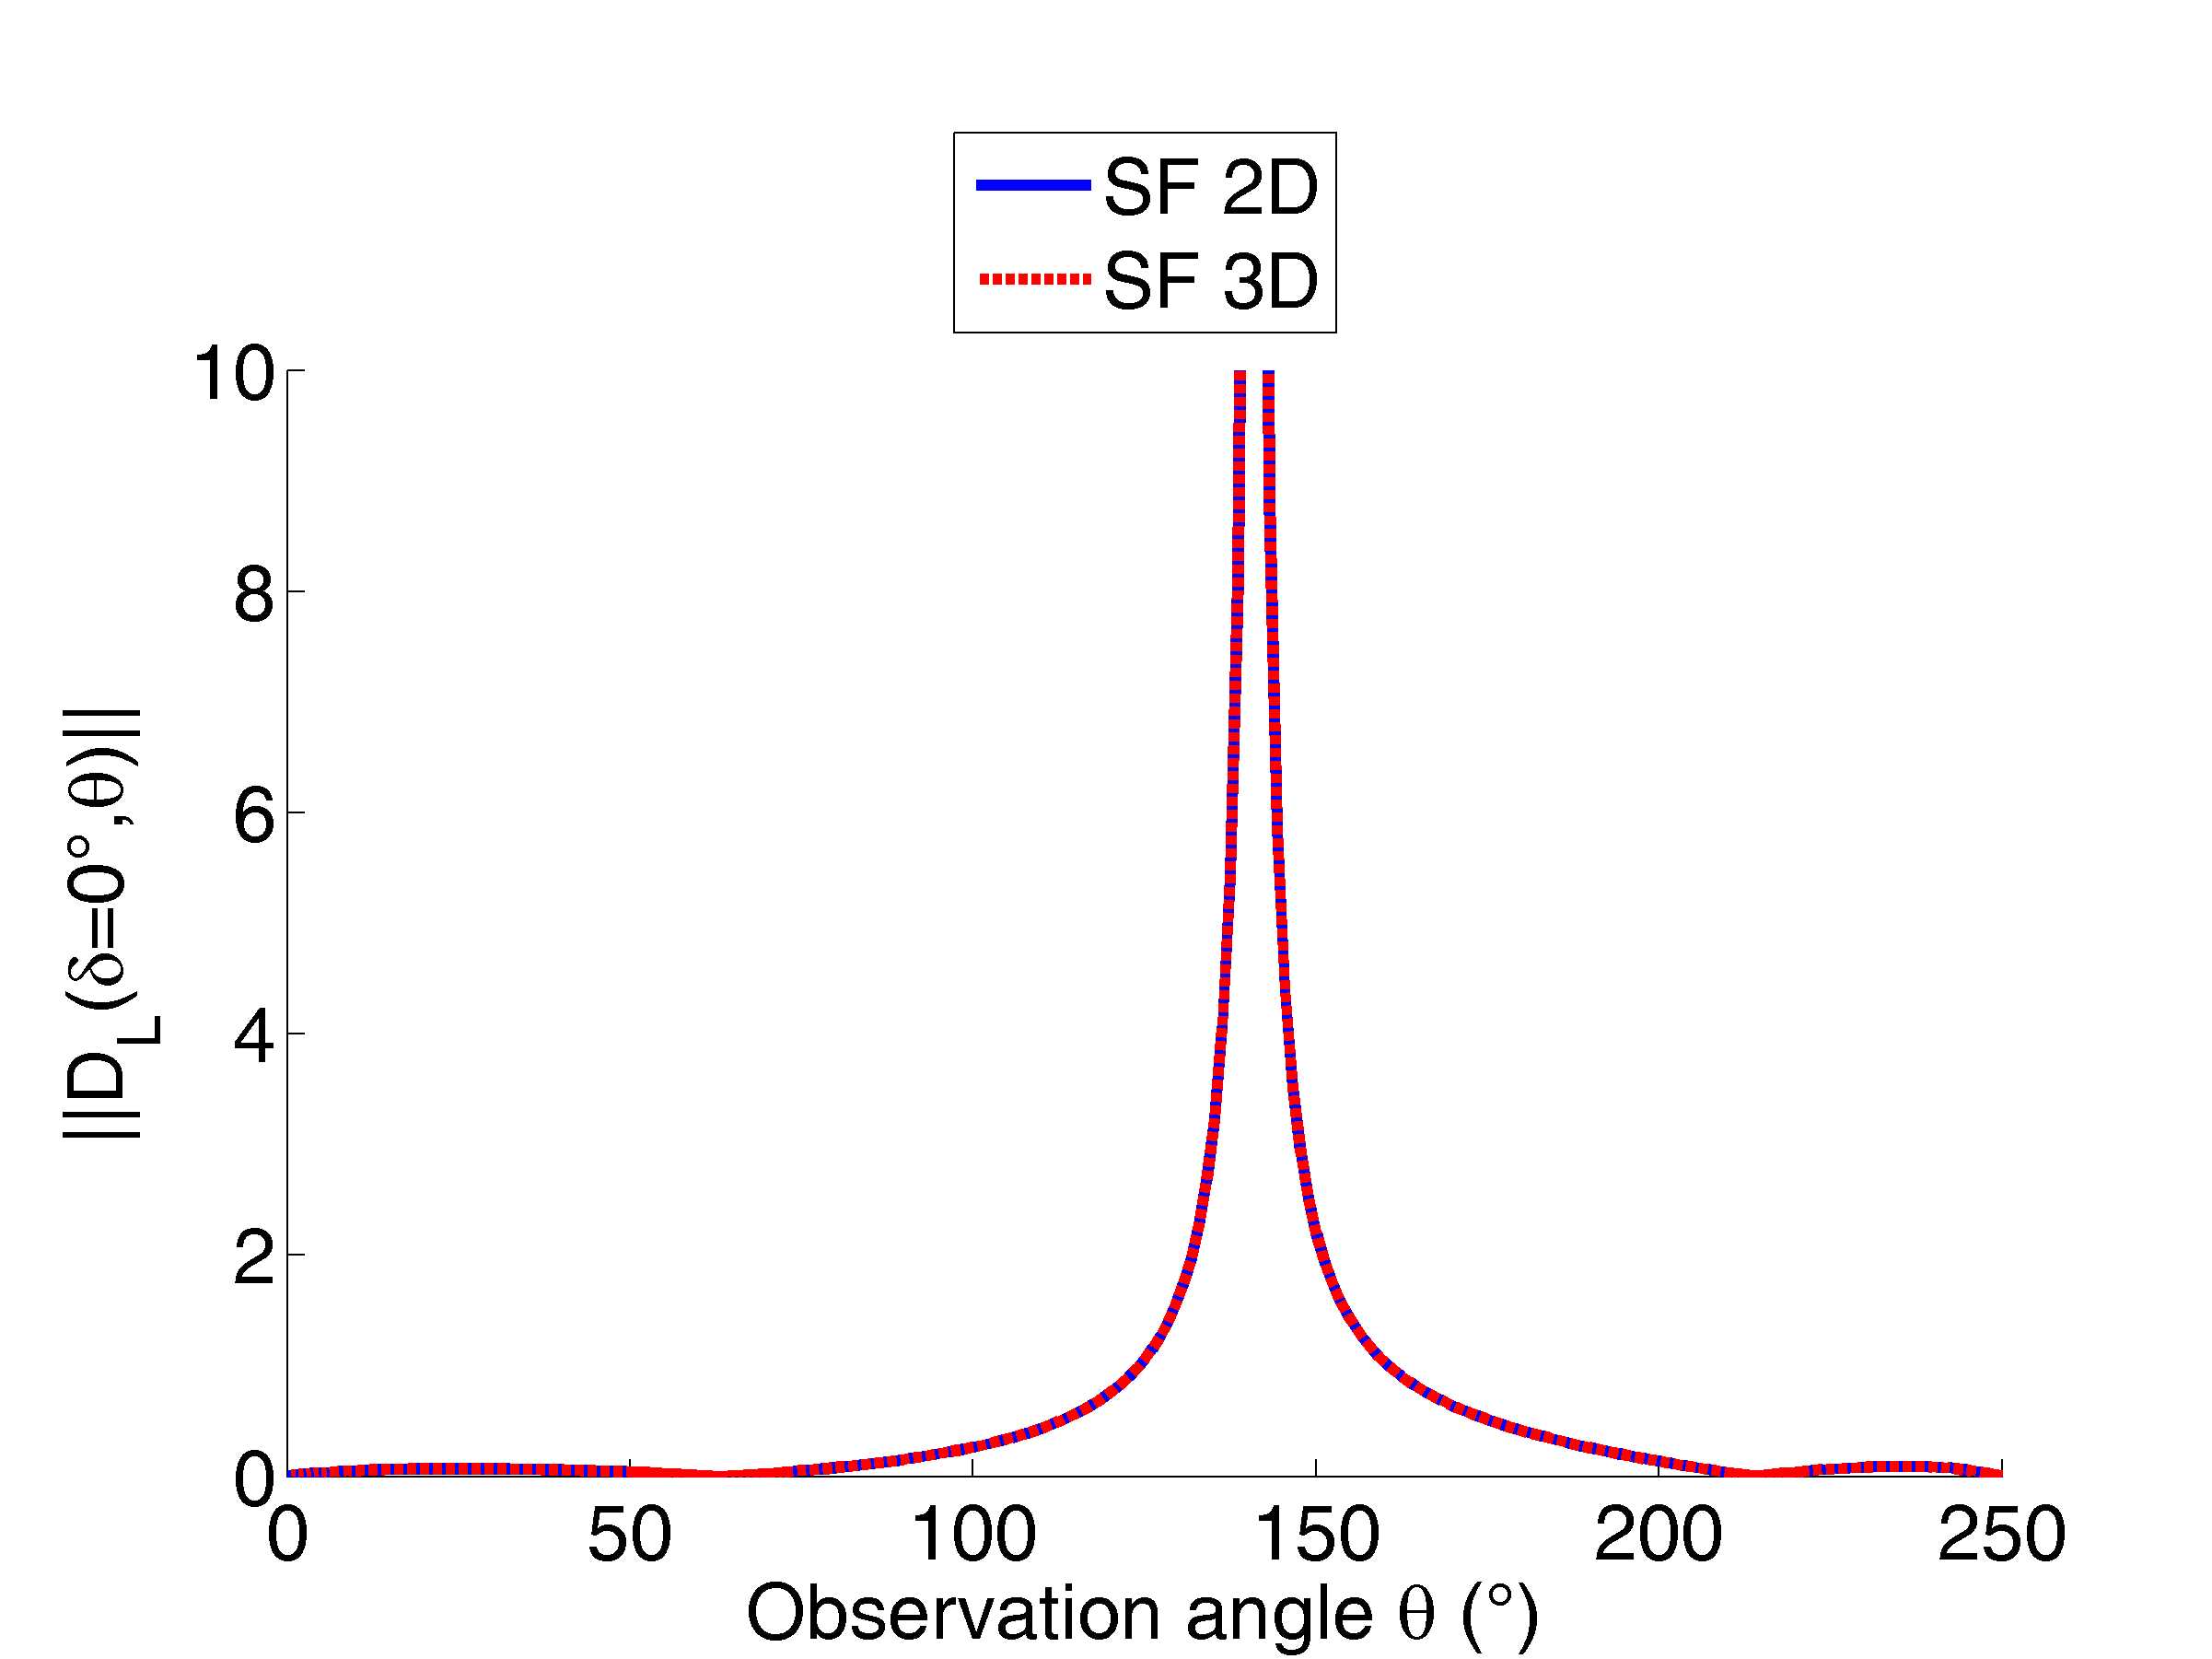
\includegraphics[width=\textwidth]{images/chapter4/XpropL_250_65_0_TH.png}
        \caption{Diffracted L wave and incident T wave.}
        \label{C4:DTL_25065}
    \end{subfigure}
    \begin{subfigure}[b]{0.44\textwidth}
        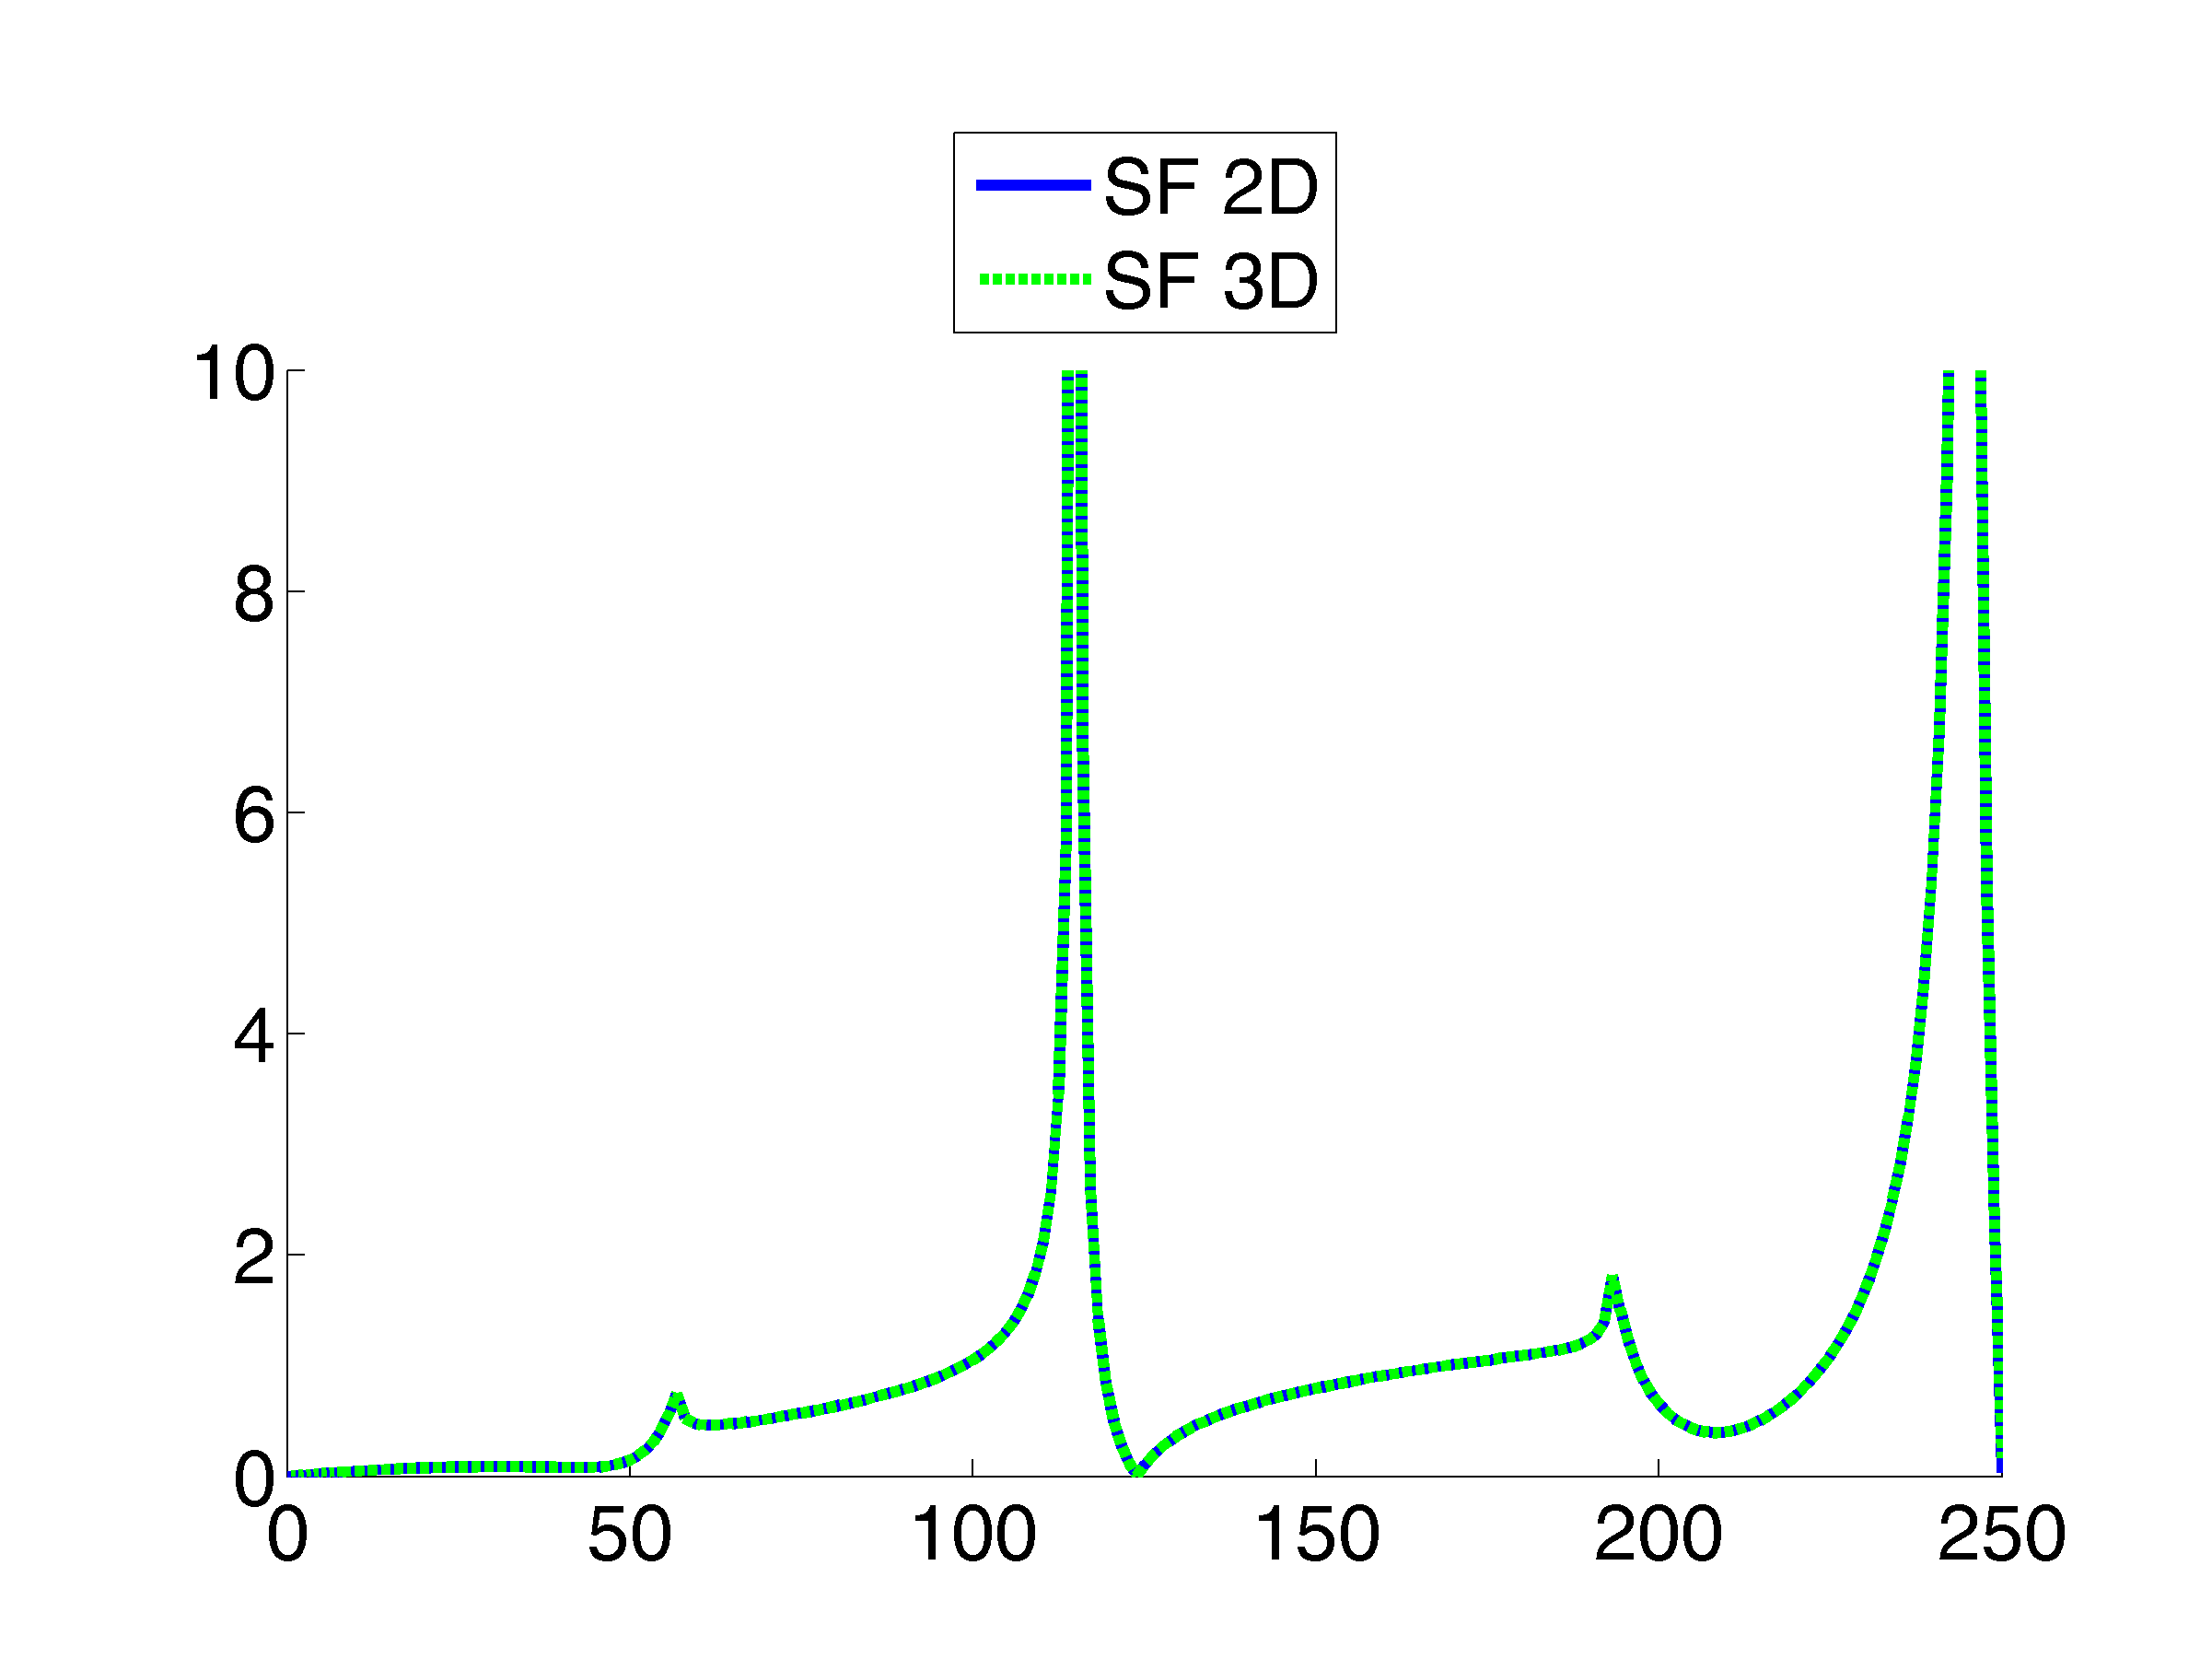
\includegraphics[width=\textwidth]{images/chapter4/XpropTH_250_65_0_TH.png}
        \caption{Diffracted and incident T waves.}
        \label{C4:DTT_25065}
     \end{subfigure}
     \caption{Diffraction coefficients for $\varphi=250^o, \theta_{inc}=65^o$}
     \label{C4:25065}
\end{figure}

Fig.~\ref{C4:25065} shows the absolute value of the diffraction coefficients obtained using the 2D and 3D \acrshort{sf} codes for a wedge of angle $\varphi=250^o$ illuminated by a wave incident with an angle $\theta_{inc}=65^o$. In Figs.~\ref{C4:DLL_25065} and \ref{C4:DTL_25065}, representing L diffraction coefficients, the thick blue line represents the results obtained using the 2D code and the dashed red line represents the results obtained using the 3D code. In Figs.~\ref{C4:DLT_25065} and \ref{C4:DTT_25065}, representing T diffraction coefficients, the thick blue line represents the results obtained using the 2D code and the dashed green line represents results obtained using the 3D code.

In all of these cases, the 2D and 3D plots are perfectly overlapping. When $\delta_{\alpha}=0^o$, the 3D code yields exactly the same results as the 2D code, which is in accord with the theoretical computations. This validates the computation of the "2D terms" (meaning the terms that are not canceled by setting $\delta_{\alpha}=0^o$)of the 3D code. The following numerical test, comparison of the 3D elastic code to Sommerfeld's analytical expression for an acoustic wave, validates a different set of terms computed by the spectral functions method.

\subsection{Acoustic limit}
In the second chapter of this manuscript, we have seen that Sommerfeld \cite{Sommerfeld} provides an analytical expression for the \acrshort{gtd} diffraction coefficient in the case of an acoustic wave incident on a wedge with Dirichlet or Neumann boundaries. This expression is still valid for 3D incidences, and the expression is provided by Keller \cite{GTD}. In the case of a wedge with Dirichlet boundaries, we have :
\begin{equation}
\begin{split}
v^{diff}(r,\theta)=D^{(Dir)}(\theta)\dfrac{e^{-ir}}{\sqrt{r\cos\delta_{\alpha}}}
\end{split}
\end{equation}
where $v^{diff}$ is the acoustic diffracted field and $D^{(Dir)}$, is given by \eqref{GTDCoeff_Dir}. For an acoustic wave, the diffraction coefficient does not depend on the incident skew angle $\delta_{\alpha}$. The dependency of the diffracted field with respect to this parameter is fully contained in the term $(r\cos\delta_{\alpha})^{-1/2}$.

The case of an acoustic wave incident on a wedge with Dirichlet boundary conditions can be mimicked using the elastic code. By setting $c_L=1$ and $c_T \rightarrow 0$ and considering incident L waves, the L diffraction coefficient should behaves like the diffraction coefficient of an acoustic wave. 

In the 3D elastic code, the wave velocities are set to $c_L=1 m.s^{-1}$ and $c_T=10^{-7} m.s^{-1}$ and the incident wave is longitudinal. The spectral functions are evaluated at $\xi=\nuti_L\cos\theta -i10^{-8}$ (a small negative imaginary part is added to ensure that the recursive equations \eqref{C4:recur} are valid) every $0,5^o$ for $0\leq\theta\leq \varphi$ and for $-90^o\leq \delta_{\alpha} \leq 90^o$ and the L diffraction coefficient is computed using \eqref{C4:Dbeta}. The results are compared to the analytical expression of the Sommerfeld diffraction coefficients for a wedge with Dirichlet boundary conditions.

\begin{figure}
\centering
\begin{subfigure}[b]{0.49\textwidth}
        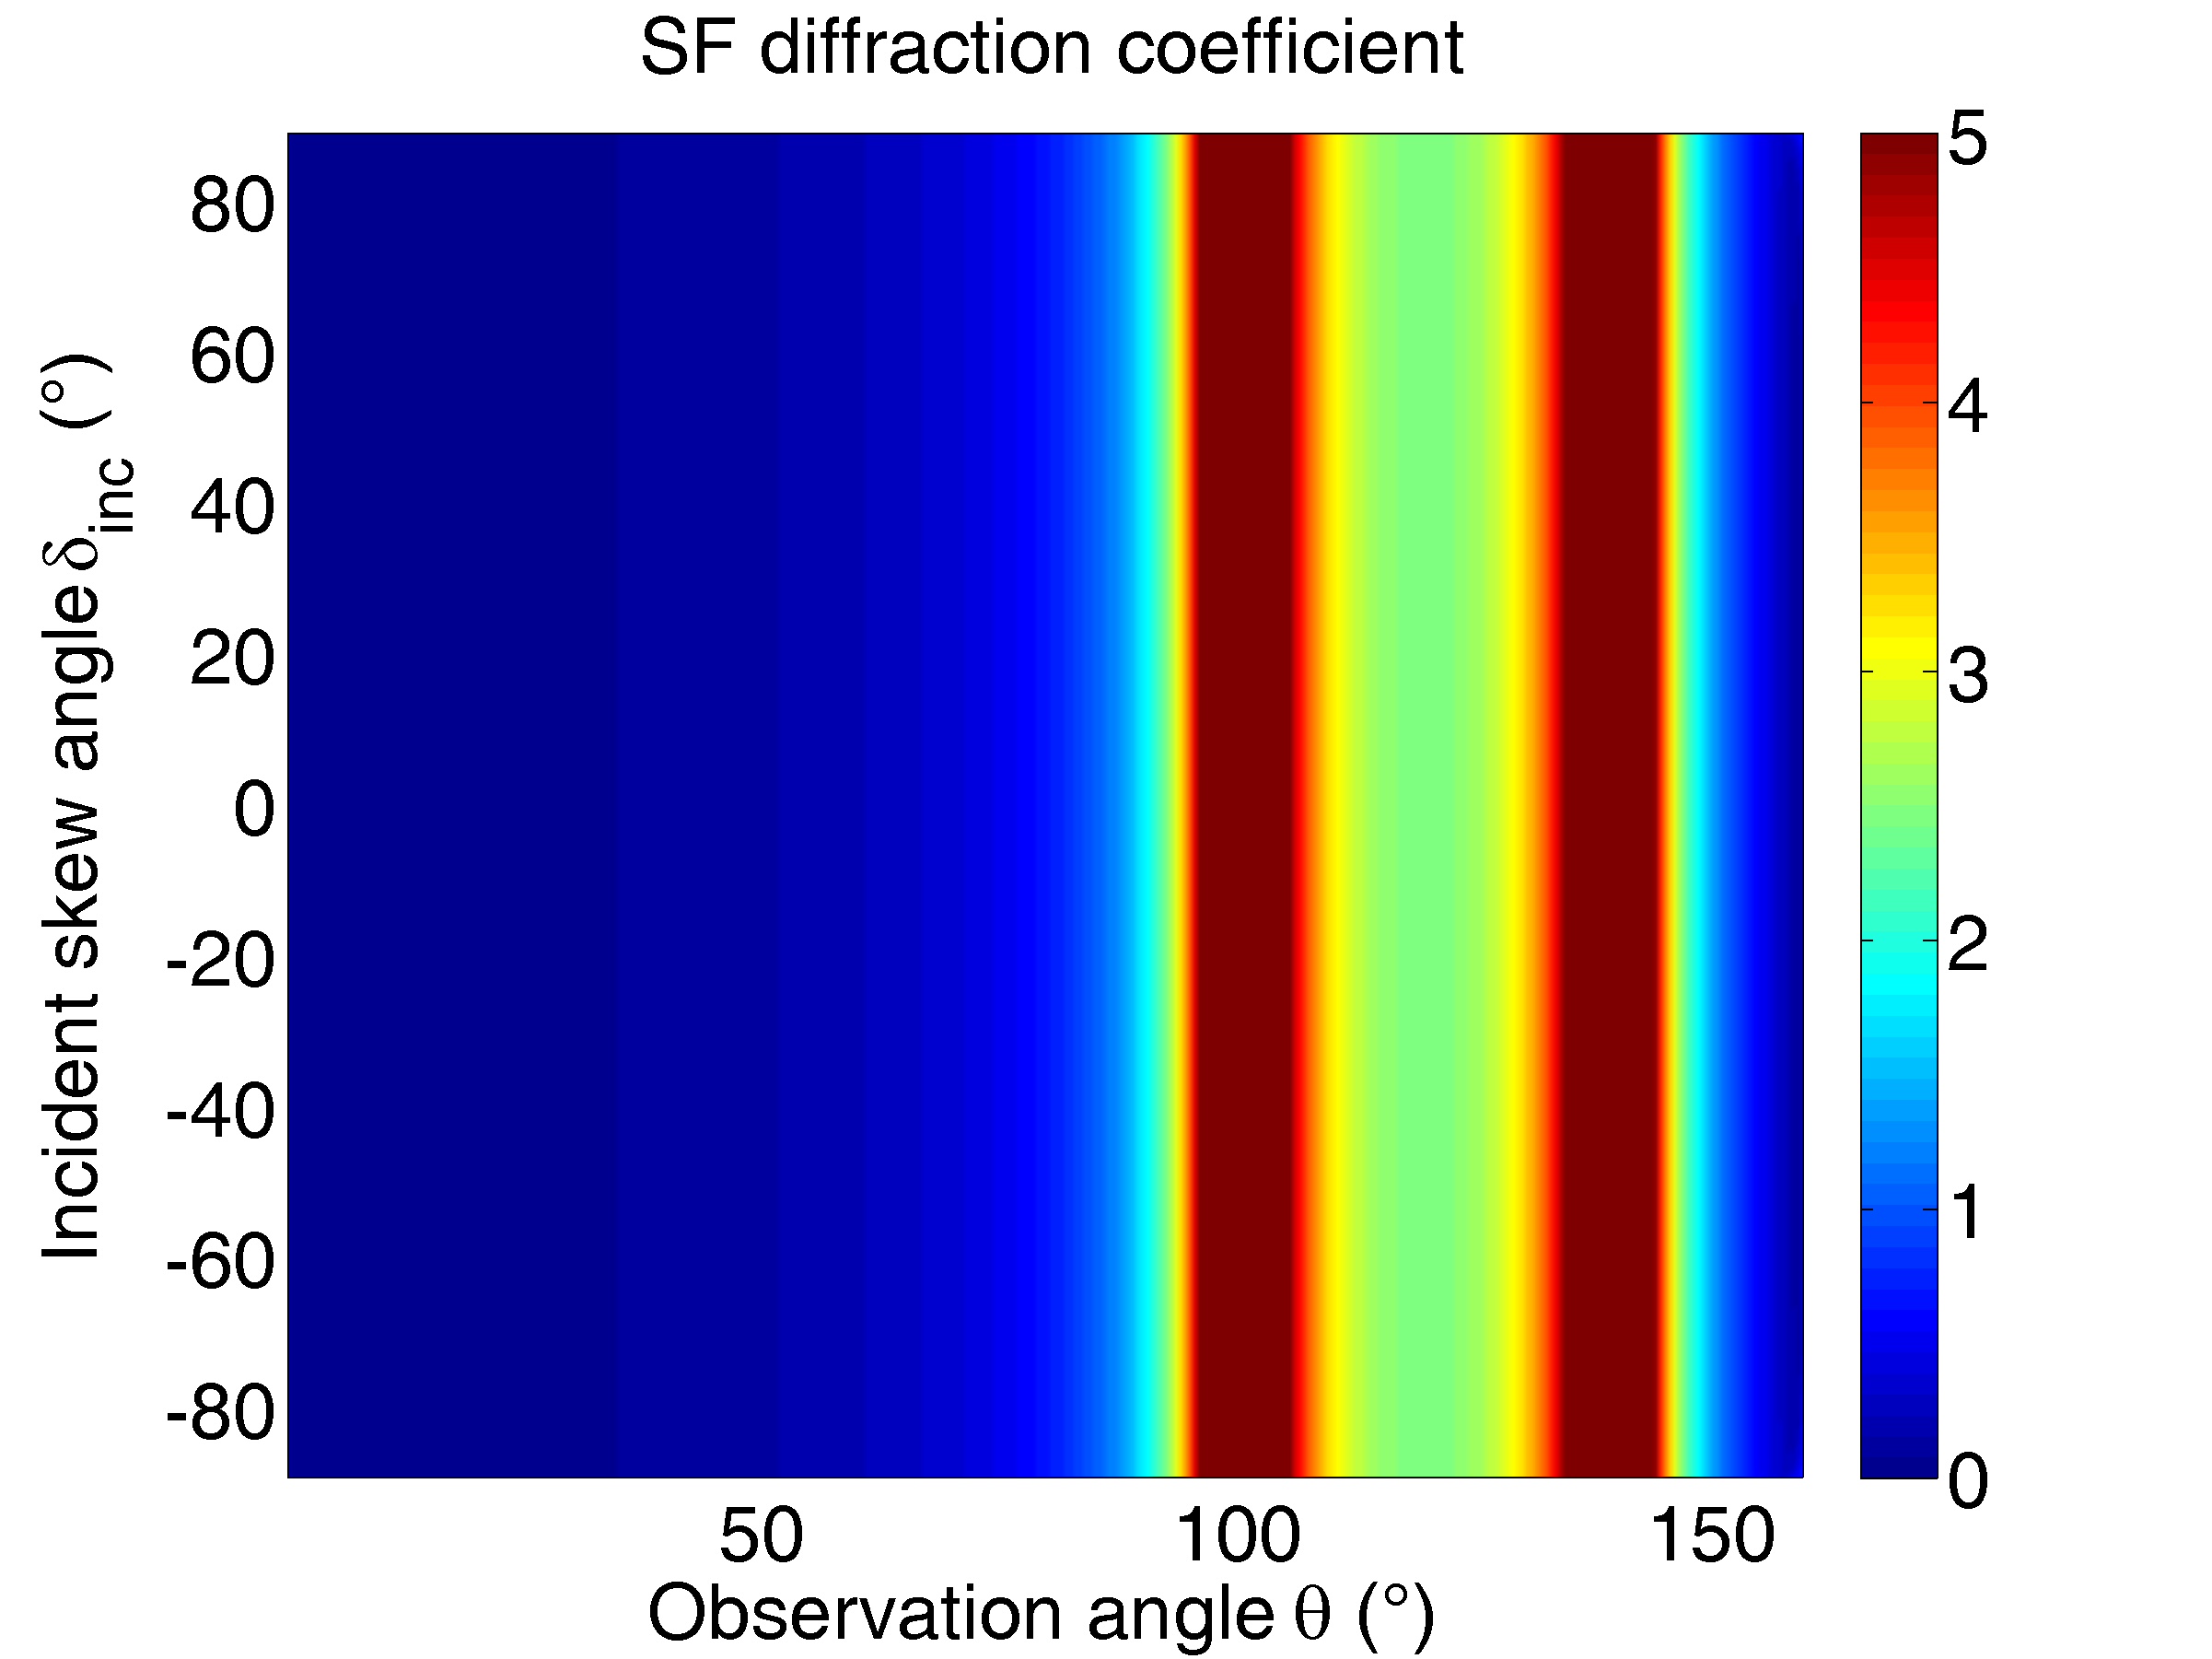
\includegraphics[width=\textwidth]{images/chapter4/Xprop_160_40.png}
        \caption{\acrshort{sf} diffraction coefficient}
        \label{C4:acSF16040}
    \end{subfigure}
\begin{subfigure}[b]{0.49\textwidth}
        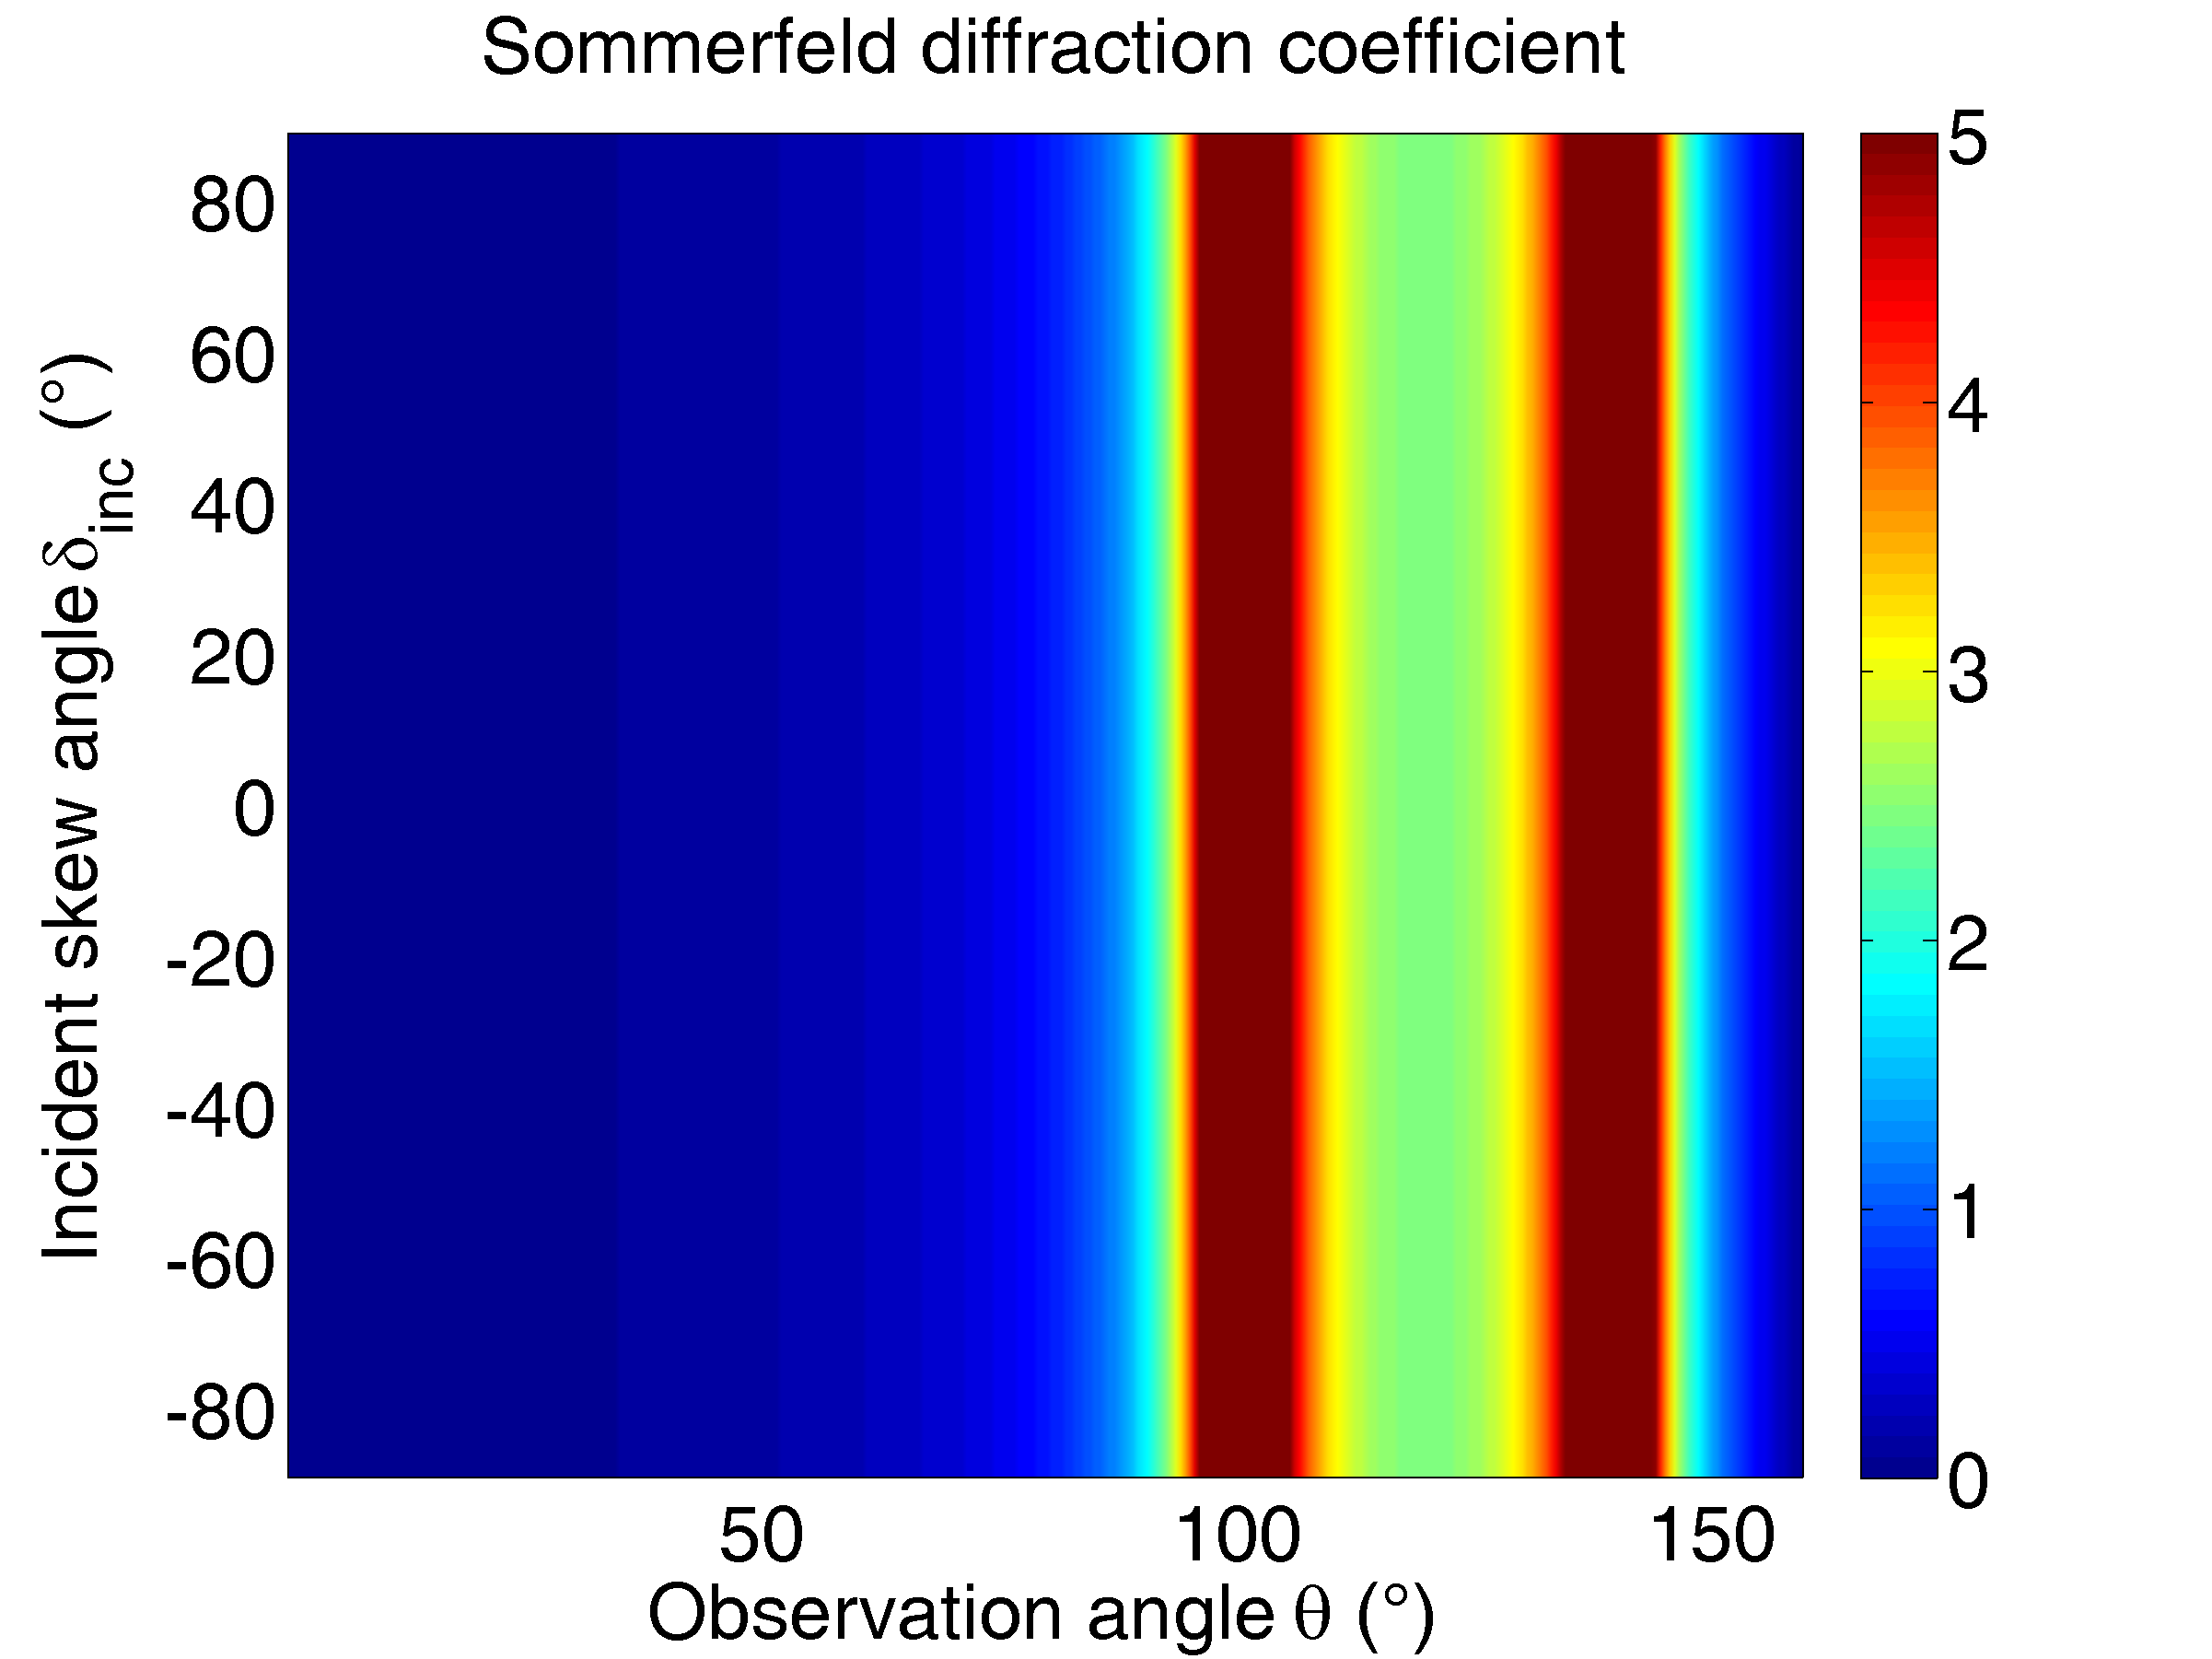
\includegraphics[width=\textwidth]{images/chapter4/Sommerfeld_160_40.png}
        \caption{Sommerfeld diffraction coefficient}
        \label{C4:Som16040}
    \end{subfigure}
\caption{Absolute value of the diffraction coefficient computed with the spectral functions and with the Sommerfeld method for a wave incident with and angle $\theta_{inc}=40^o$ on a wedge of angle $\varphi=160^o$}
\label{C4:ac16040}
\end{figure}

Fig.~\ref{C4:ac16040} shows the absolute value of the diffraction coefficient obtained using the \acrshort{sf} code (Fig.~\ref{C4:acSF16040}) and with Sommerfeld's analytical expression (Fig.~\ref{C4:Som16040}) for a wave incident with an angle $\theta_{\alpha}=40^o$ on a wedge of angle $\varphi=160^o$. These are computed for various incident skew angles $\delta_{\alpha}$ to check that the \acrshort{sf} diffraction coefficient is independent of this parameter, as it should be in the acoustic case. The horizontal axis corresponds to the observation angle $\theta$, the vertical axis corresponds to the incident skew angle $\delta_{\alpha}$ and the magnitude of the diffraction coefficients is represented in color in the $(\theta,\delta_{\alpha})$ plane. Both figures appear to be identical and are invariant by vertical translation (meaning that the coefficients do not depend on the angle $\delta_{\alpha}$). The diffraction coefficients can therefore be plotted for a single skew angle, without loss of generality. 

\begin{figure}
\centering
\begin{subfigure}[b]{0.49\textwidth}
        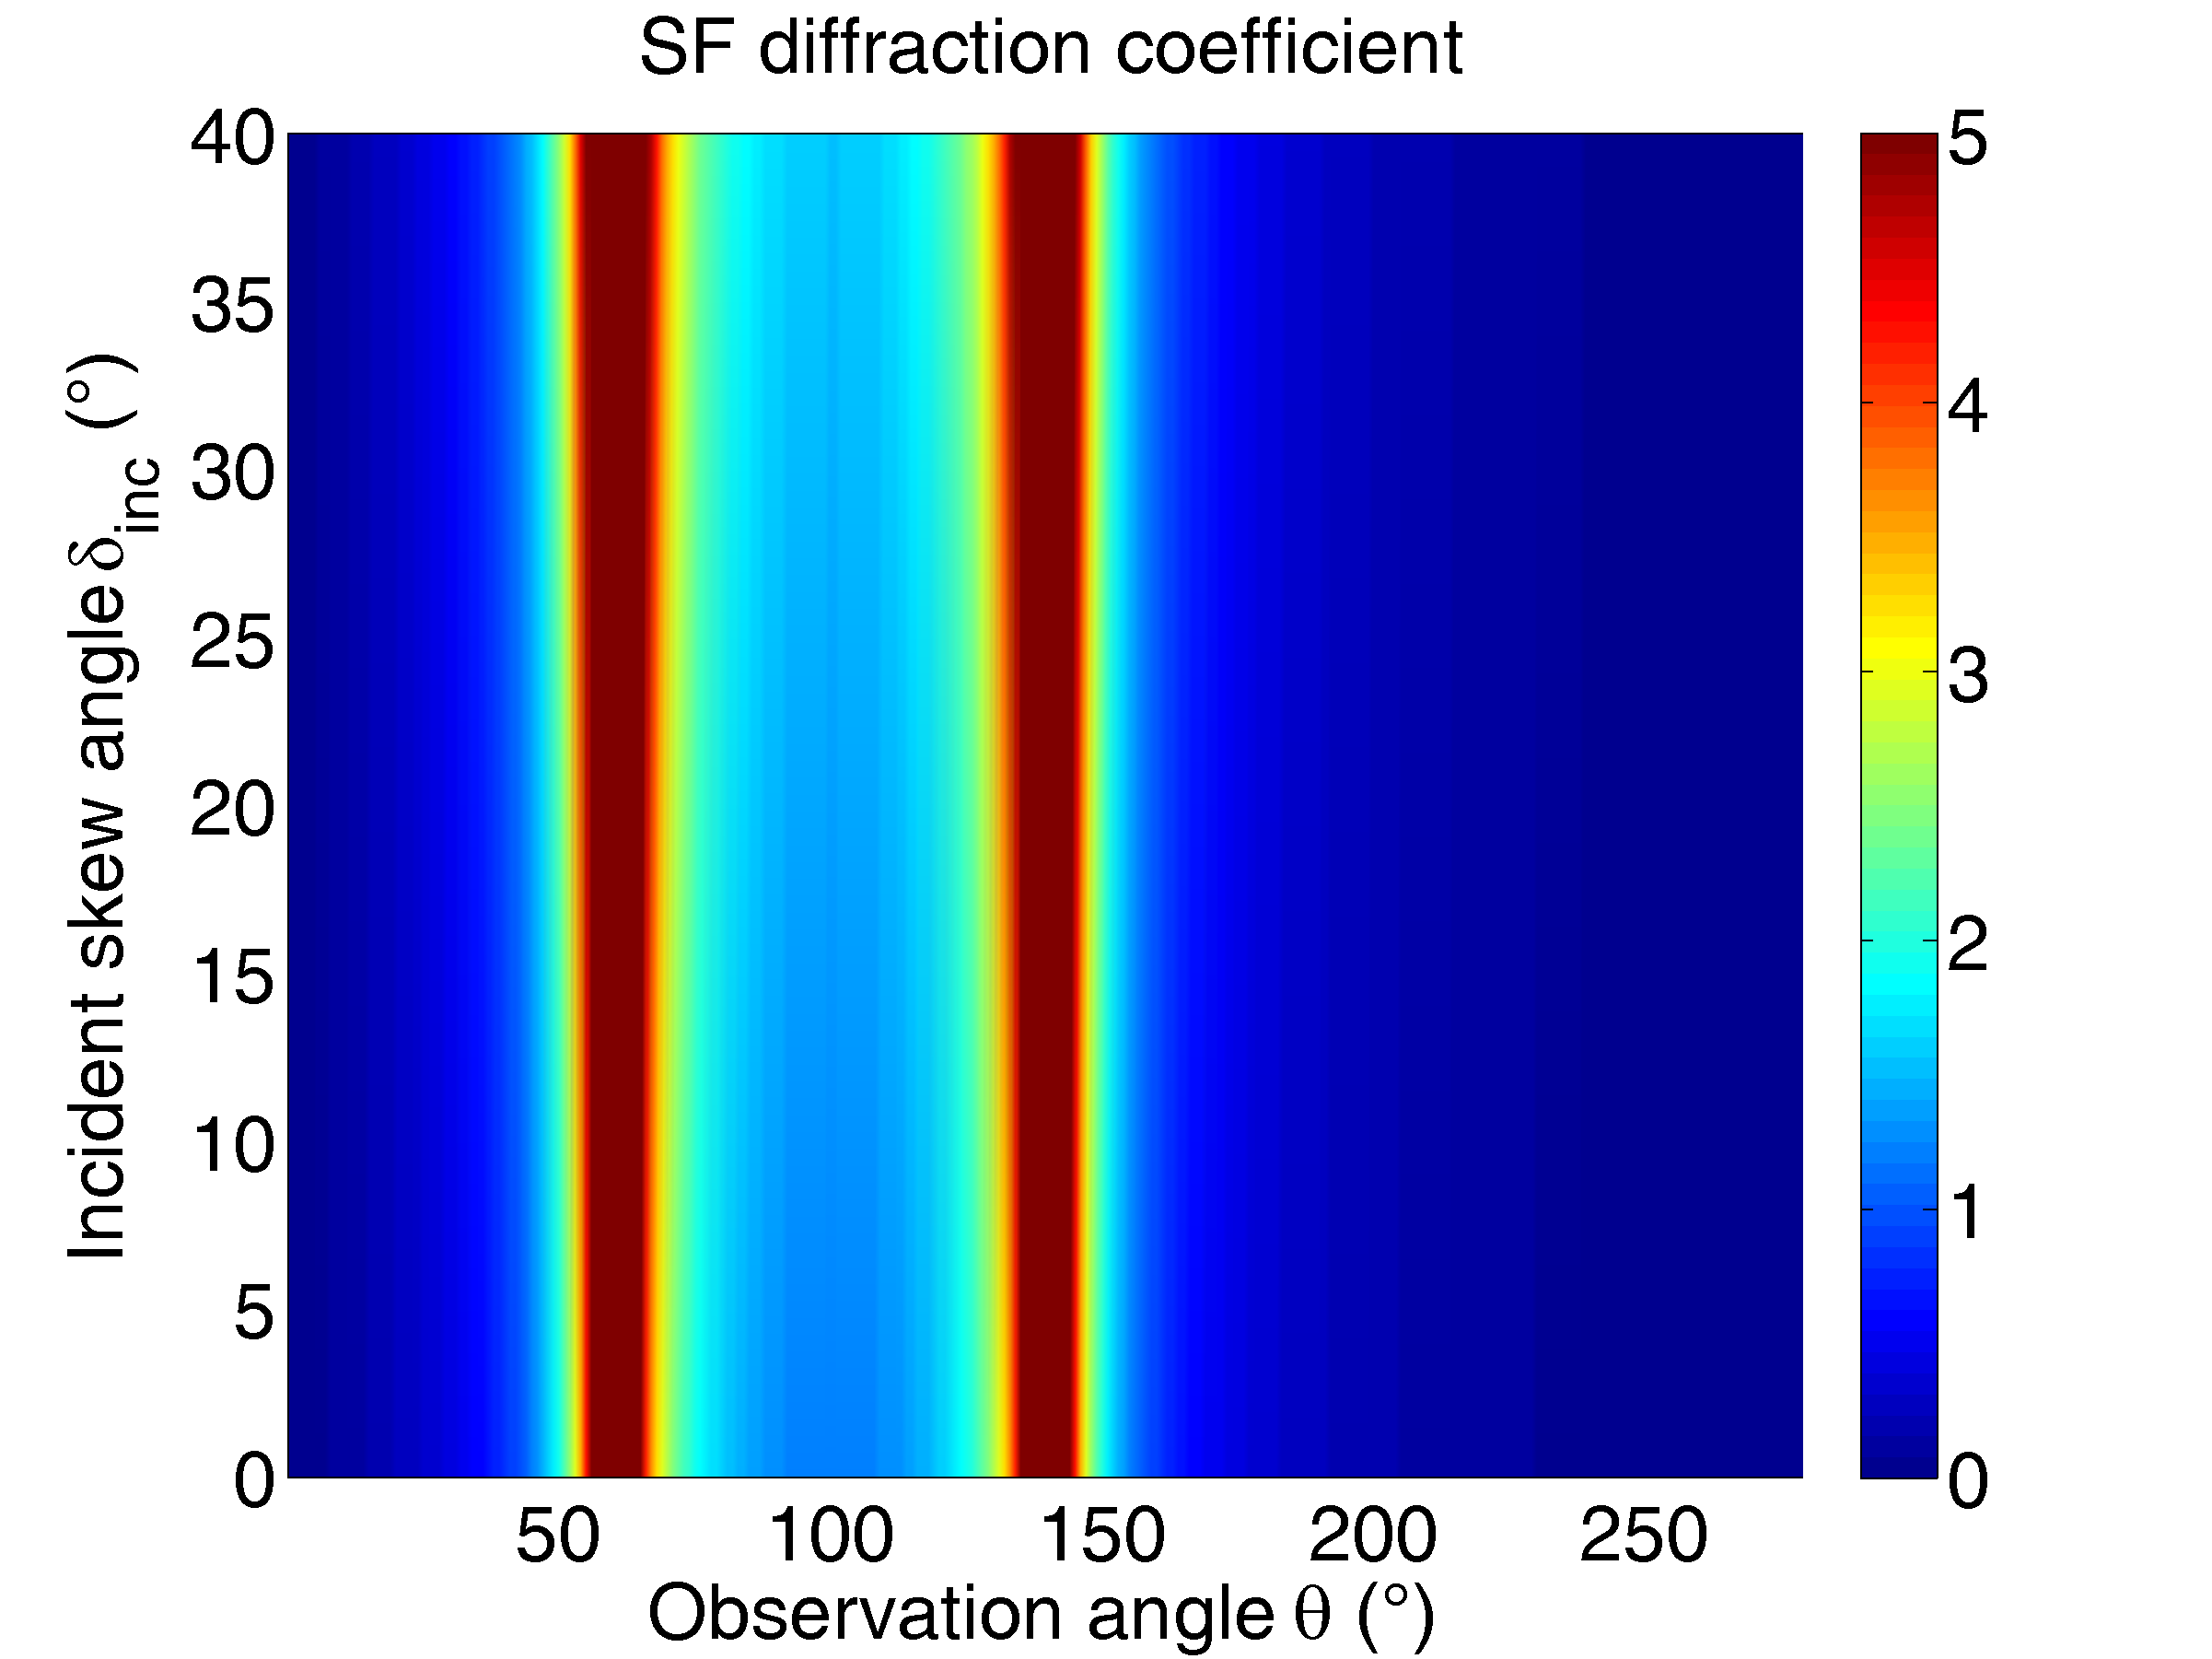
\includegraphics[width=\textwidth]{images/chapter4/Xprop_280_239.png}
        \caption{\acrshort{sf} diffraction coefficient}
        \label{C4:acSF280240}
    \end{subfigure}
\begin{subfigure}[b]{0.49\textwidth}
        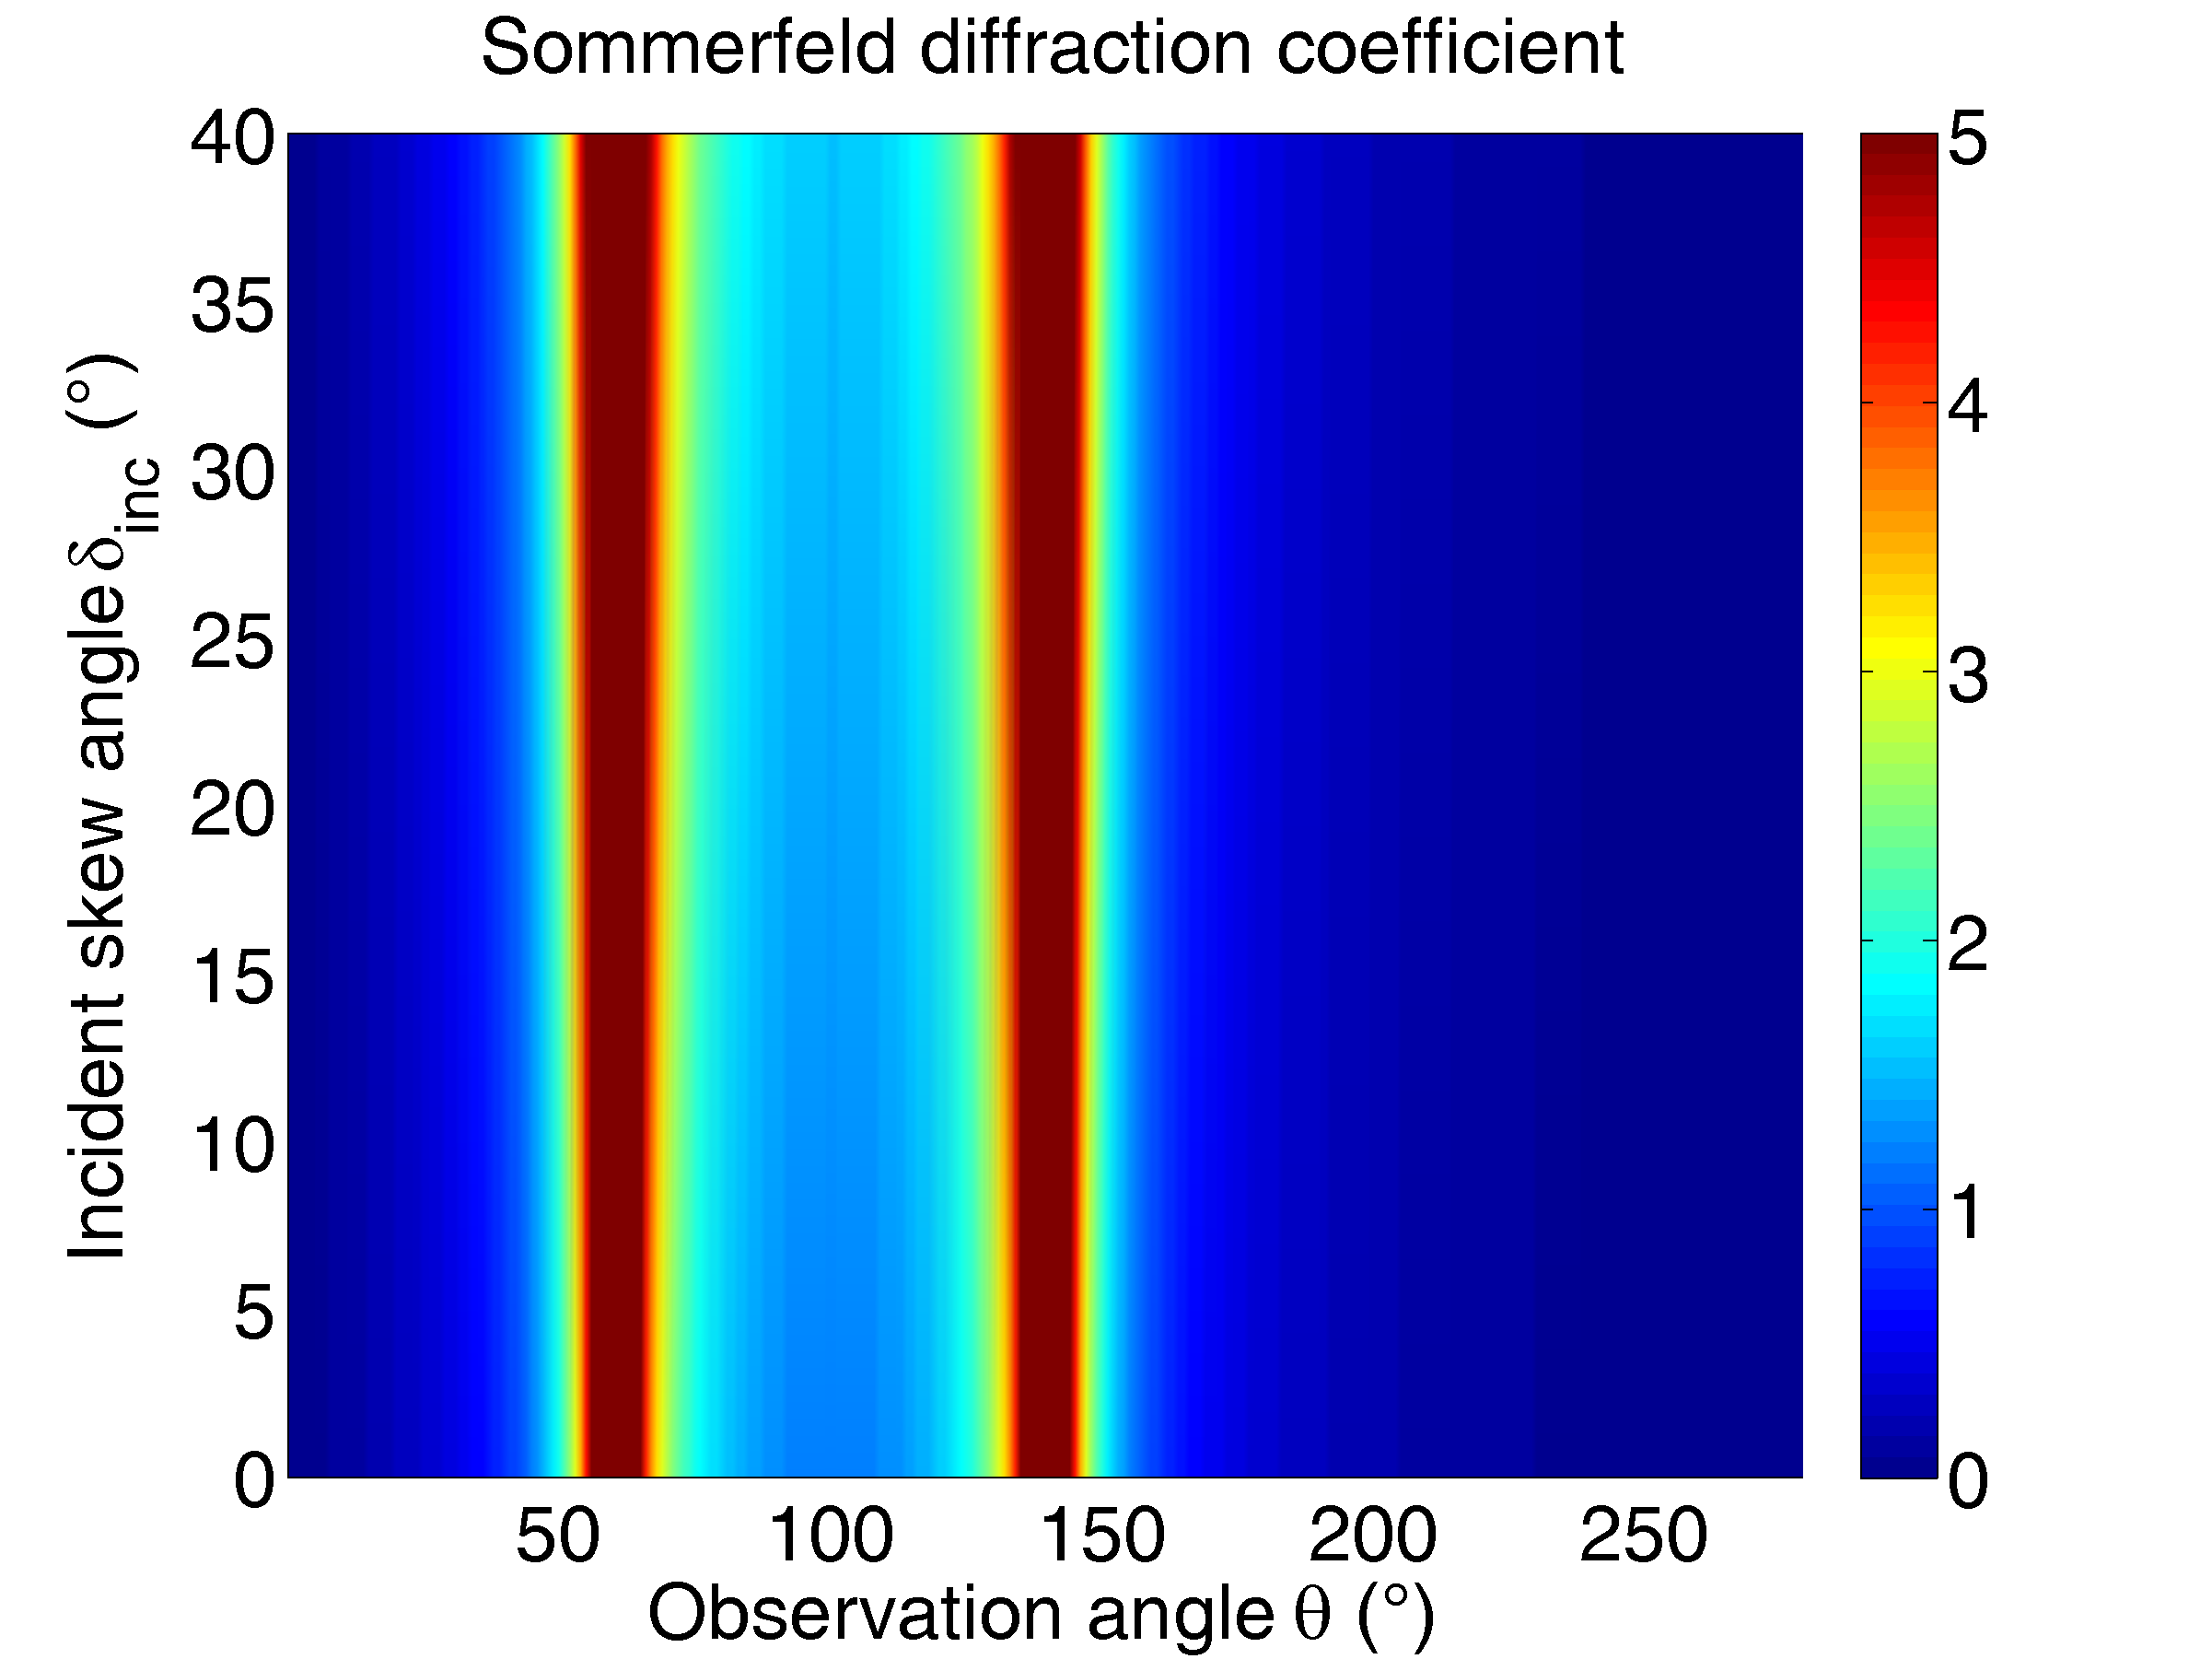
\includegraphics[width=\textwidth]{images/chapter4/Sommerfeld_280_239.png}
        \caption{Sommerfeld diffraction coefficient}
        \label{C4:Som280240}
    \end{subfigure}
\caption{Absolute value of the diffraction coefficient computed with the spectral functions and with the Sommerfeld method for a wave incident with and angle $\theta_{inc}=240^o$ on a wedge of angle $\varphi=280^o$}
\label{C4:ac280240}
\end{figure}

Fig.~\ref{C4:ac280240} shows the absolute value of the diffraction coefficient obtained using the \acrshort{sf} code (Fig.~\ref{C4:acSF280240}) and with Sommerfeld's analytical expression (Fig.~\ref{C4:Som280240}) for a wave incident with an angle $\theta_{\alpha}=240^o$ on a wedge of angle $\varphi=280^o$. These are computed for various incident skew angles $\delta_{\alpha}$ to check that the \acrshort{sf} diffraction coefficient is independent of this parameter, as it should be in the acoustic case. The horizontal axis corresponds to the observation angle $\theta$, the vertical axis corresponds to the incident skew angle $\delta_{\alpha}$ and the magnitude of the diffraction coefficients is represented in color in the $(\theta,\delta_{\alpha})$ plane. Both figures appear to be identical and are invariant by vertical translation (meaning that the coefficients do not depend on the angle $\delta_{\alpha}$). The diffraction coefficients can therefore be plotted for a single skew angle, without loss of generality. 

\begin{figure}
\centering
\begin{subfigure}[b]{0.49\textwidth}
        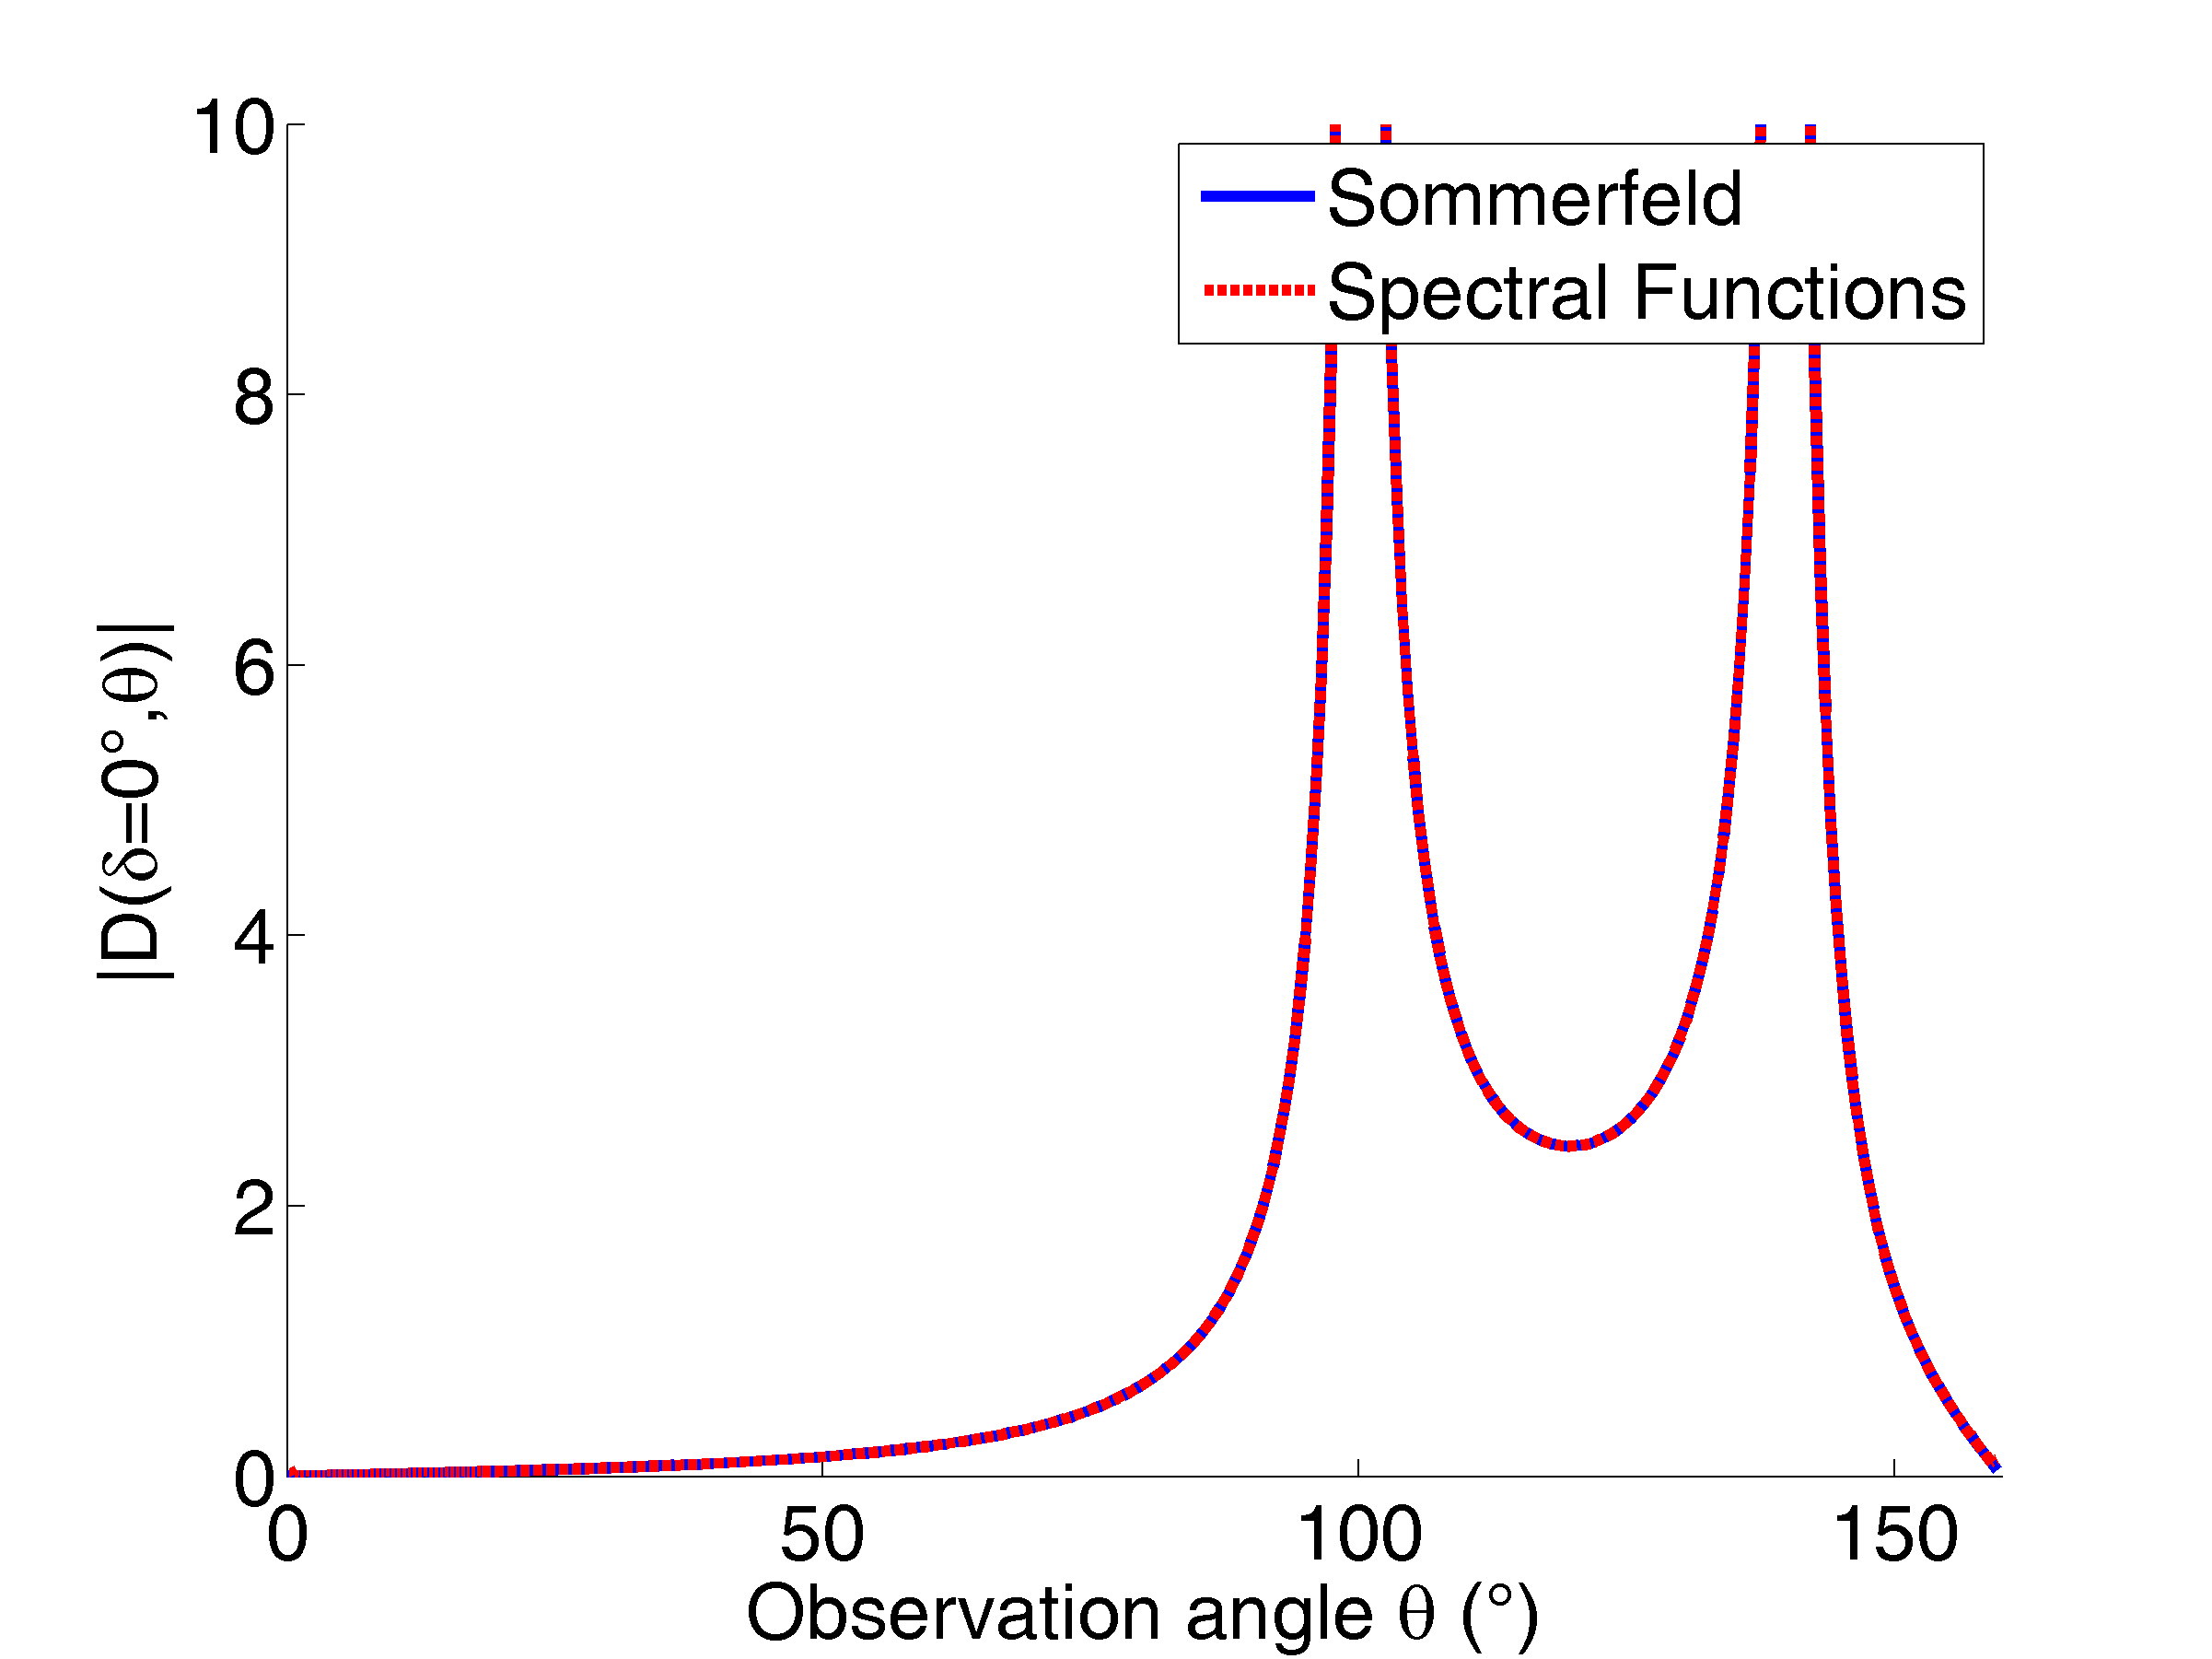
\includegraphics[width=\textwidth]{images/chapter4/D_160_40_0.png}
        \caption{$\varphi=160^o,  \, \, \theta_{inc}=40^o$}
        \label{C4:compac16040}
    \end{subfigure}
\begin{subfigure}[b]{0.49\textwidth}
        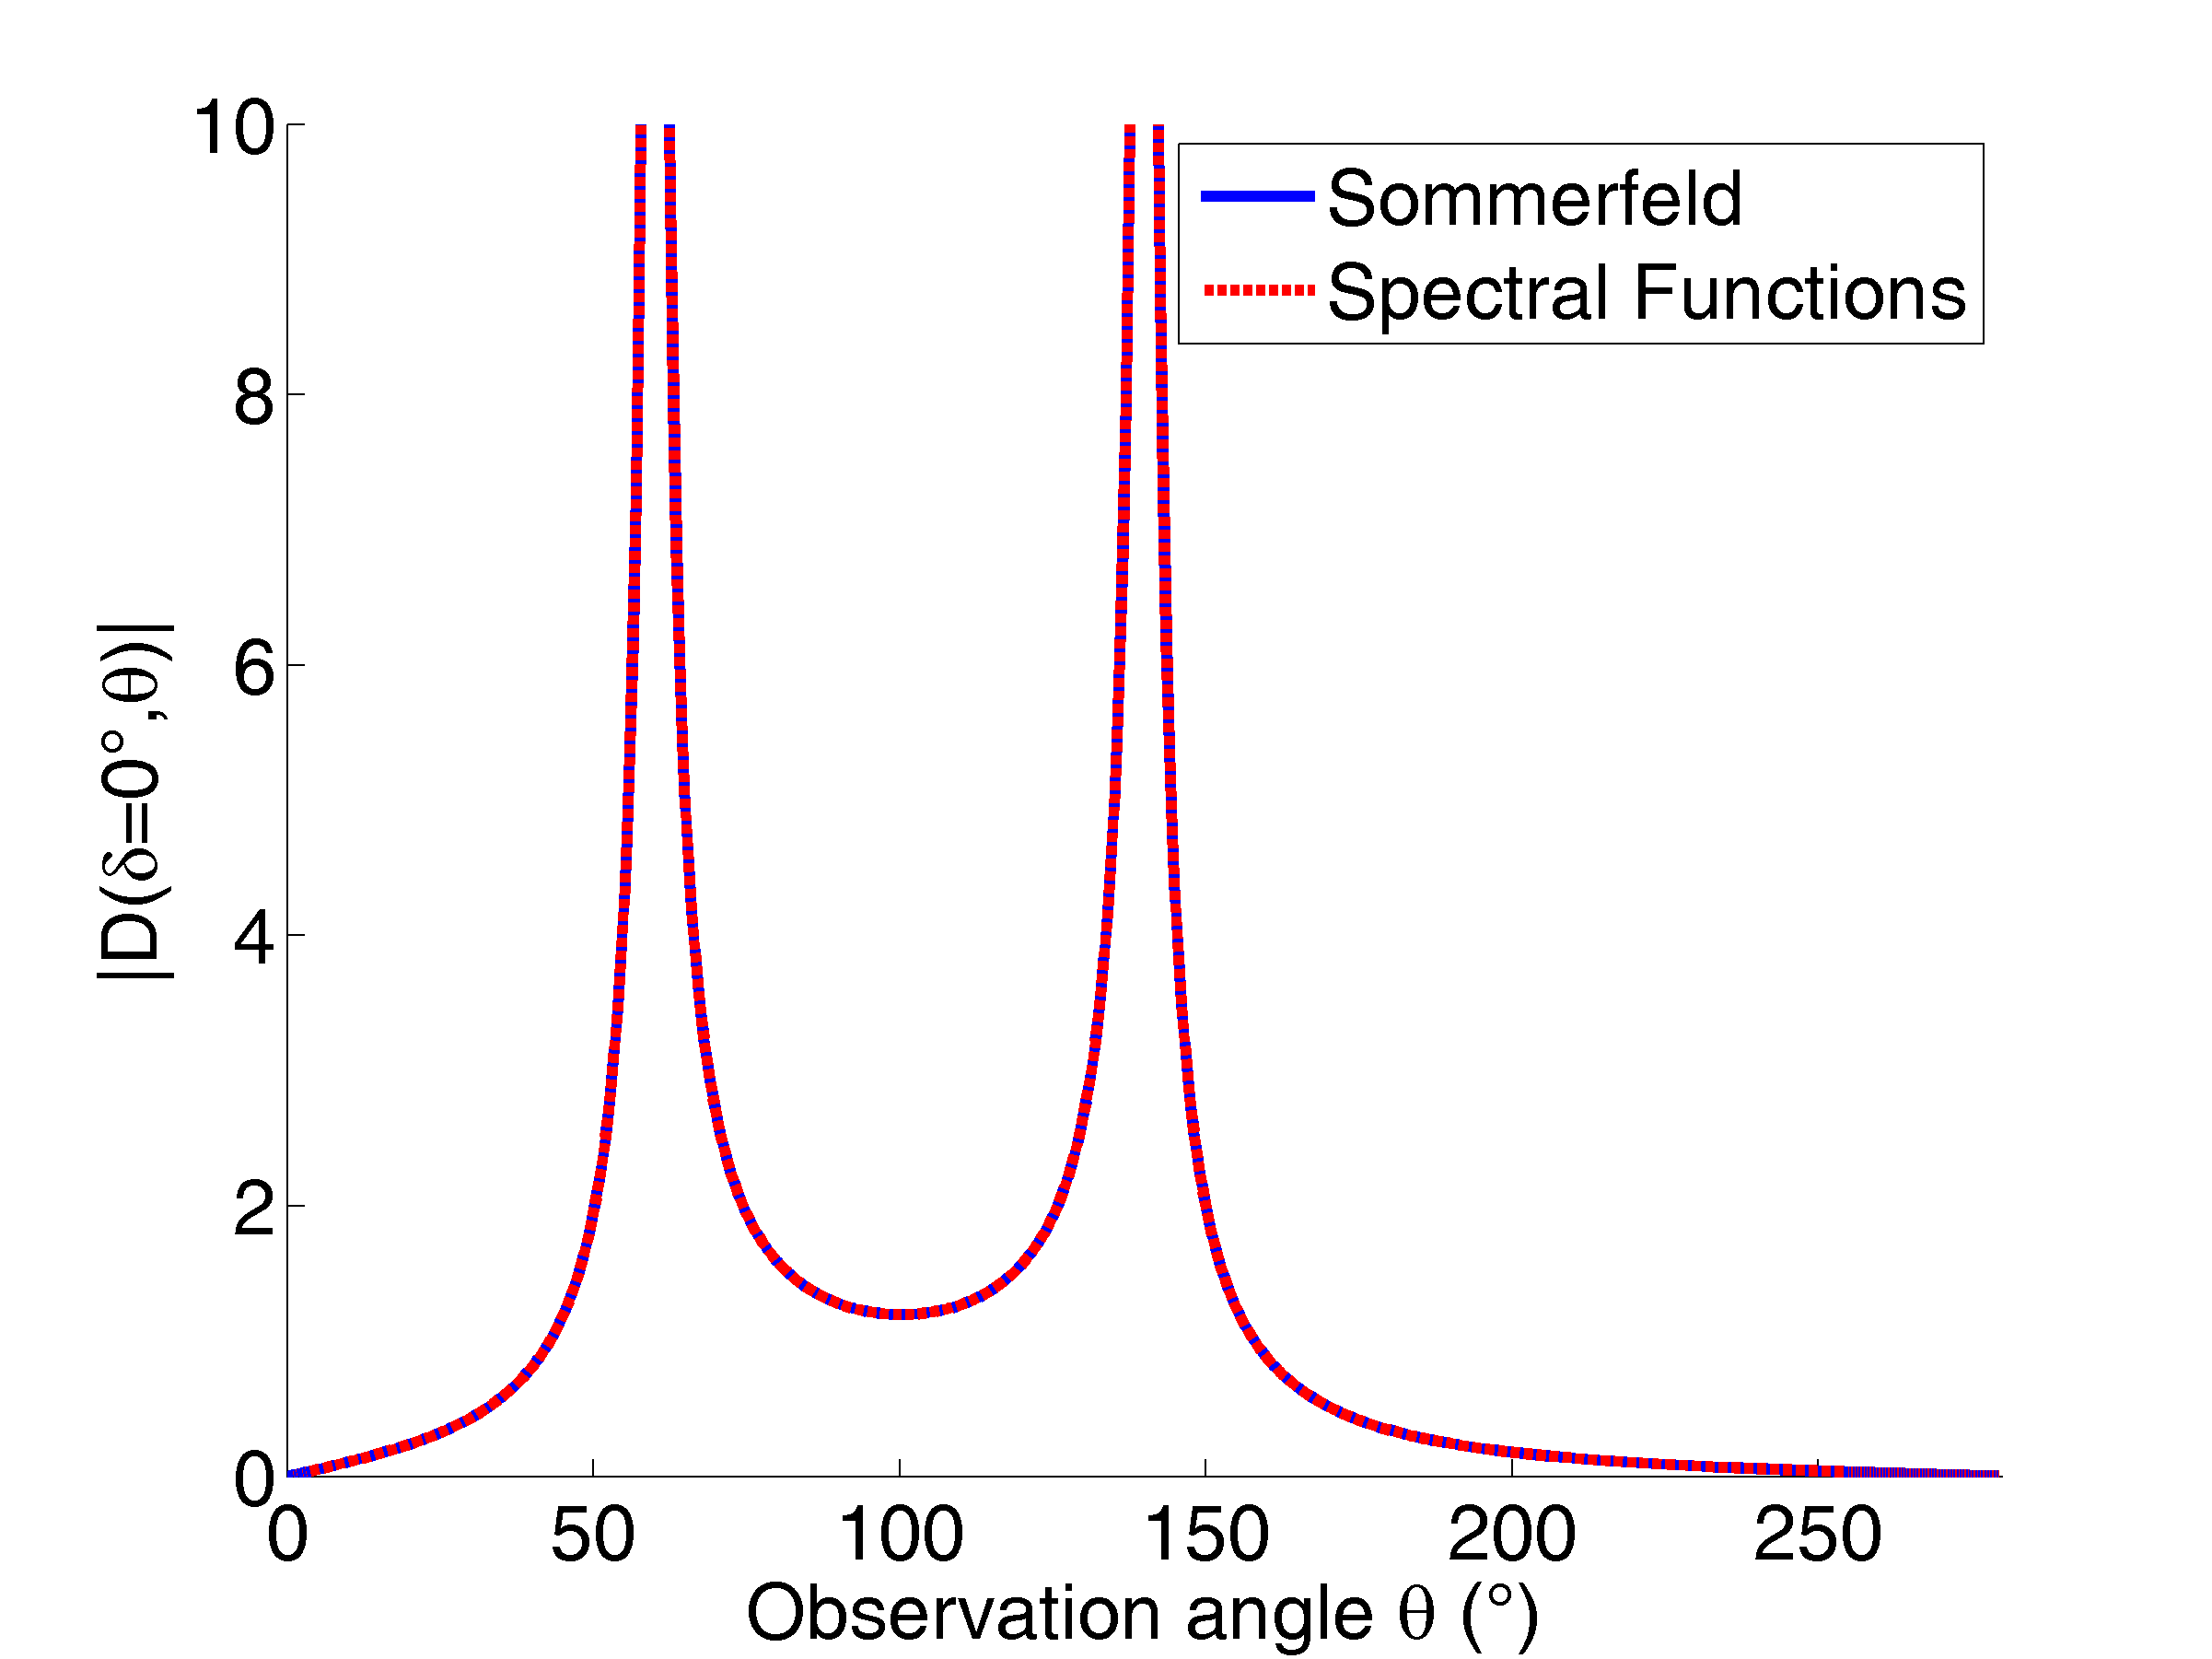
\includegraphics[width=\textwidth]{images/chapter4/D_280_239_0.png}
        \caption{$\varphi=280^o, \, \, \theta_{inc}=240^o$}
        \label{C4:compac280240}
    \end{subfigure}
\caption{Absolute value of the diffraction coefficient computed with the spectral functions and with the Sommerfeld method for $\delta_{inc}=0^o$.}
\label{C4:compac}
\end{figure}

Fig.~\ref{C4:compac} shows the absolute value of the diffraction coefficient, plotted for $\delta_{\alpha}=0^o$ for a wave incident with an angle $\theta_{\alpha}=40^o$ on a wedge of angle $\varphi=160^o$ (see Fig.~\ref{C4:compac16040}) and for a wave incident with an angle $\theta_{\alpha}=240^o$ on a wedge of angle $\varphi=280^o$ (see Fig.~\ref{C4:compac280240}). In both figures, the thick blue line is the solution computed using Sommerfeld's analytical expression and the dashed red line is the result obtained using acoustic limit of the 3D \acrshort{sf} code. Both lines are perfectly overlapping.

The "acoustic limit" of the 3D elastic code is thus validated for wedge angles lower and higher than $\pi$. This shows that the terms appearing in the evaluation of the spectral functions that depend on $\nuti_T$ tend to $0$ when transversal wave velocity tends to $0$ and that the terms that depend on $\nuti_L$ are computed correctly. 

\subsection{Verification of the regular part for an infinite plane}
In the case where $\varphi=\pi$, the wedge degenerates into an infinite plane and there is no diffracted wave. The regular part of the spectral functions, which is the part of the solution corresponding to the diffraction phenomena, vanishes and we should have, for $j=1,2$ :
\begin{equation}
||\mathbb{U}_j||=0 \hspace{1em} %\rm and \hspace{1em} ||\mathbb{X}_j||=0
\end{equation}
Verifying that this is the case provides a check on the lengthy computations of the explicit expressions of operators $\mathbb{D}(\cdot,\cdot)$ and $\mathbb{T}(\cdot,\cdot)$. Since the value of $||\mathbb{U}_j||$ does not depend on the observation angle $\theta$, only the skew incidence angle $\delta_{\alpha}$ varies.

\begin{figure}
\centering
\begin{subfigure}[b]{0.32\textwidth}
        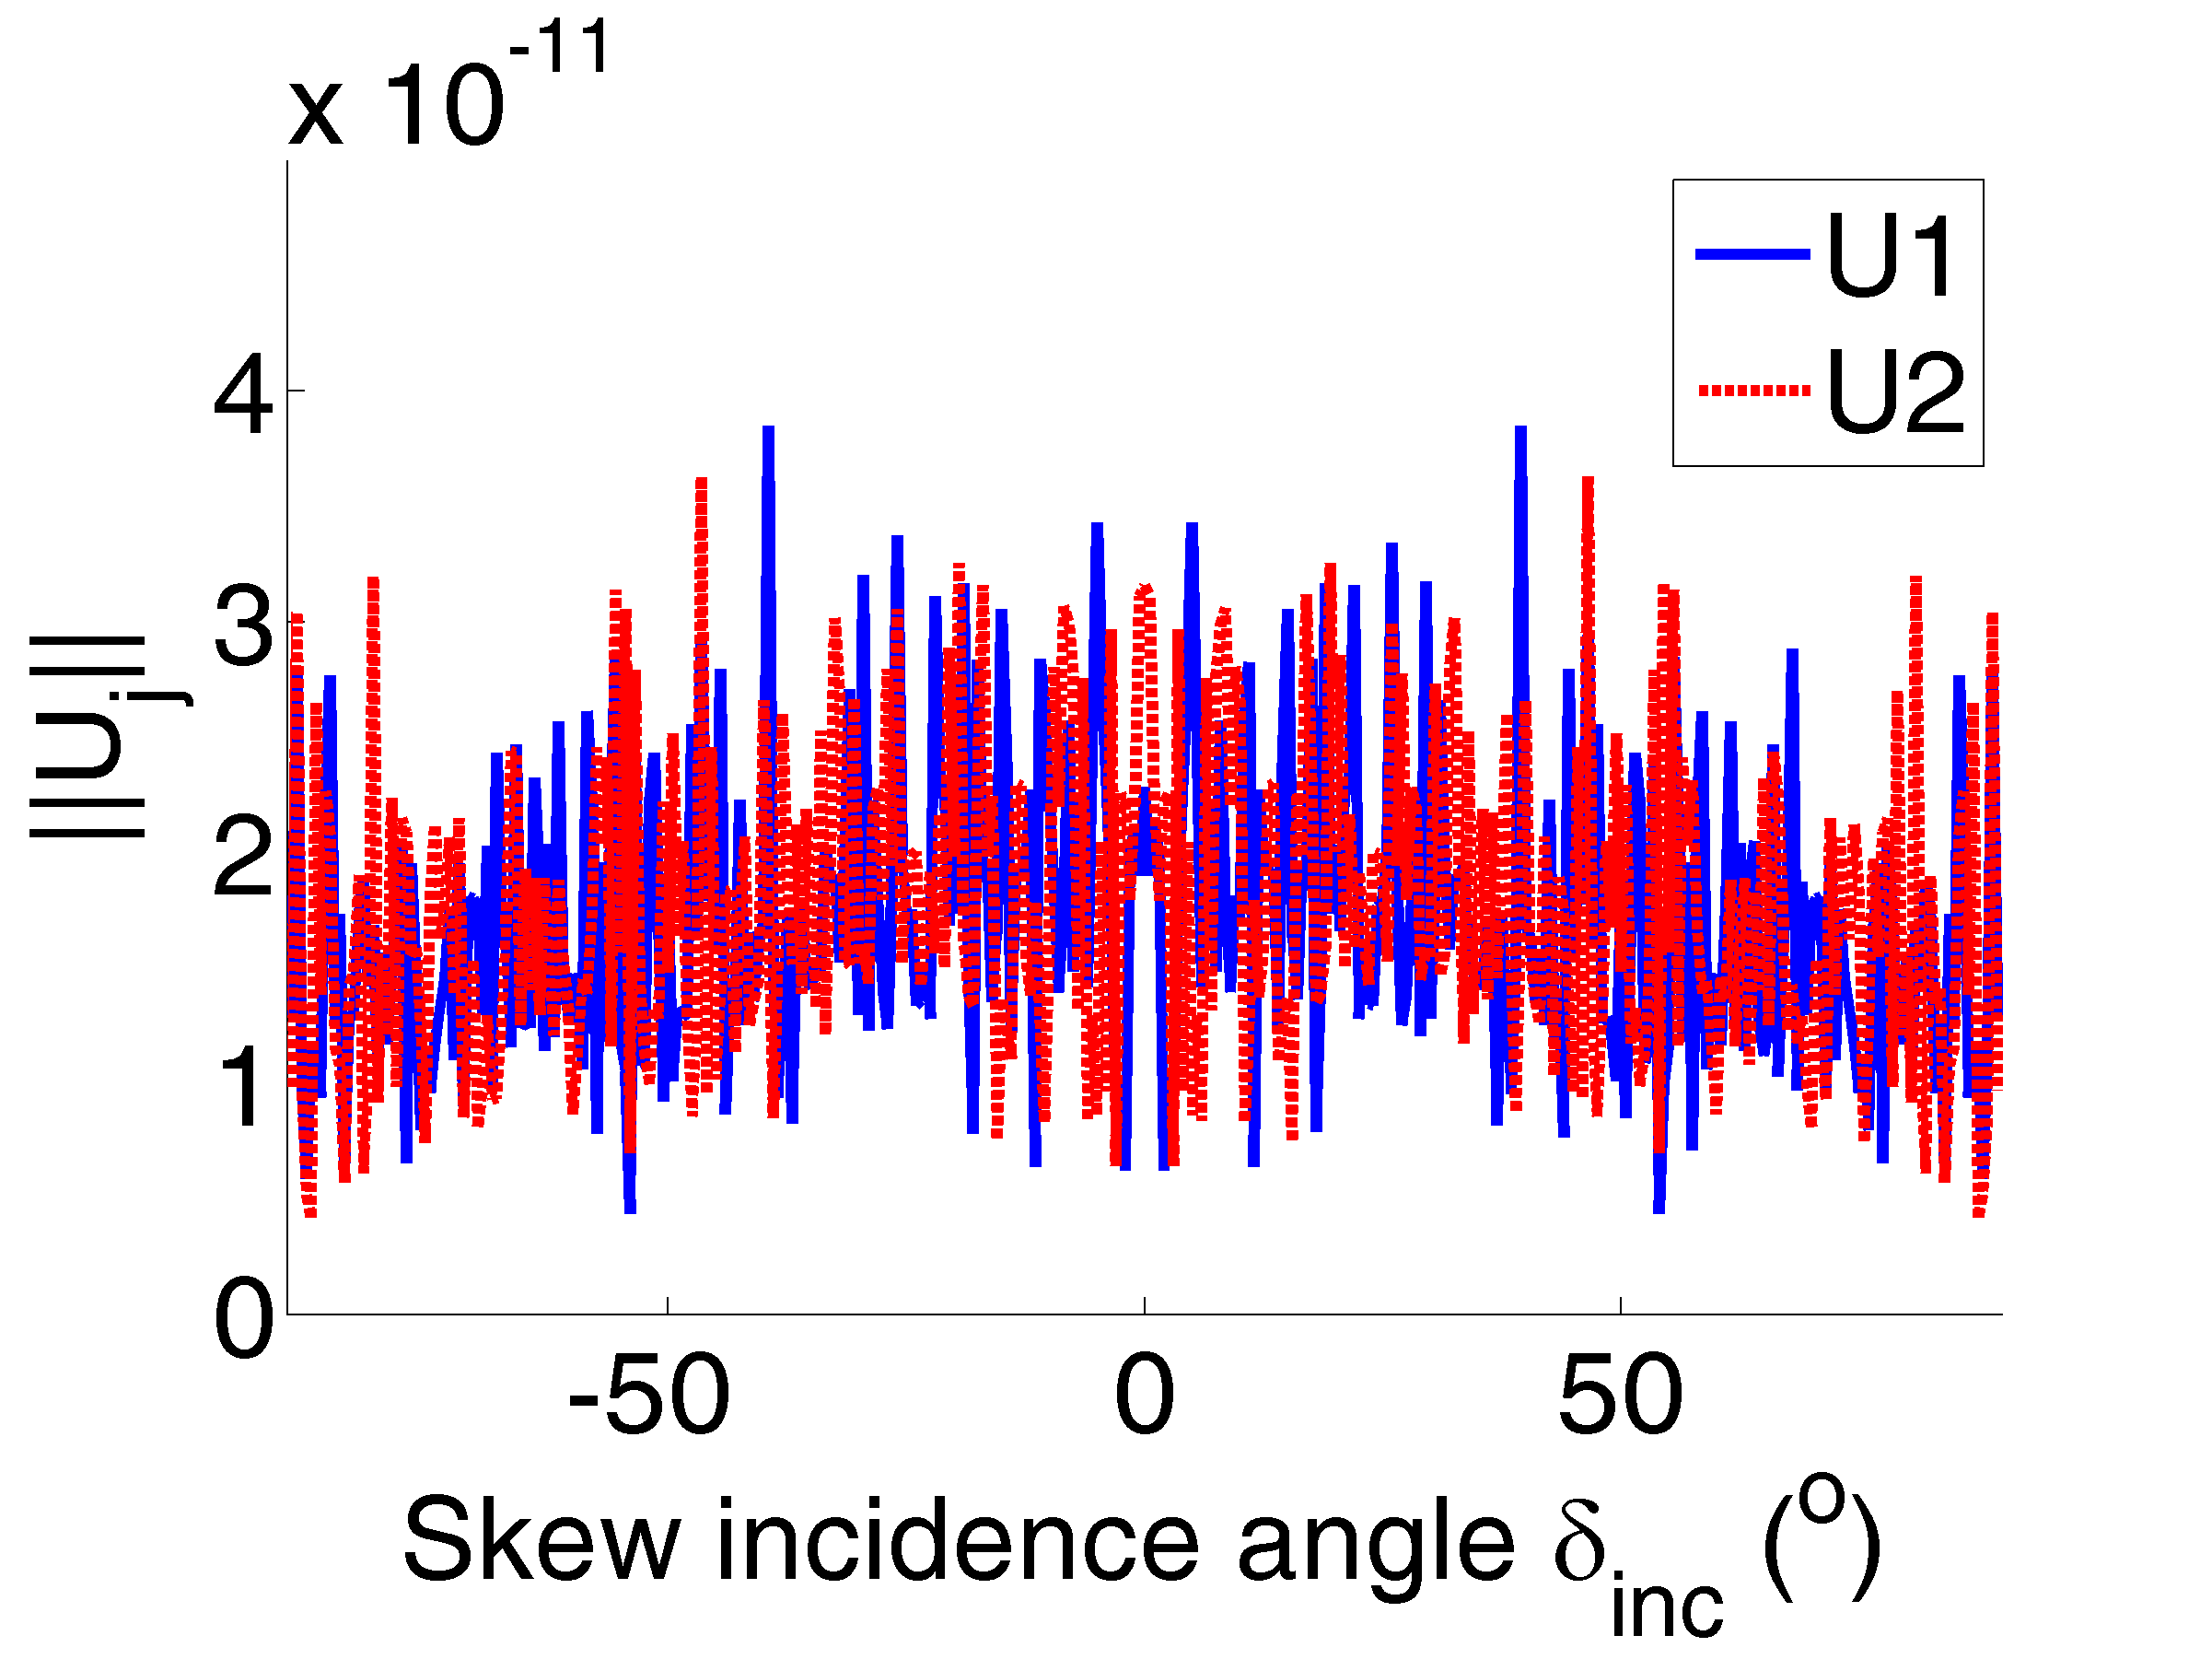
\includegraphics[width=\textwidth]{images/chapter4/Resultats_3D/U1L_180_50.png}
        \caption{Incident L wave}
        \label{Resultat_3D:U1L}
    \end{subfigure}
\begin{subfigure}[b]{0.32\textwidth}
        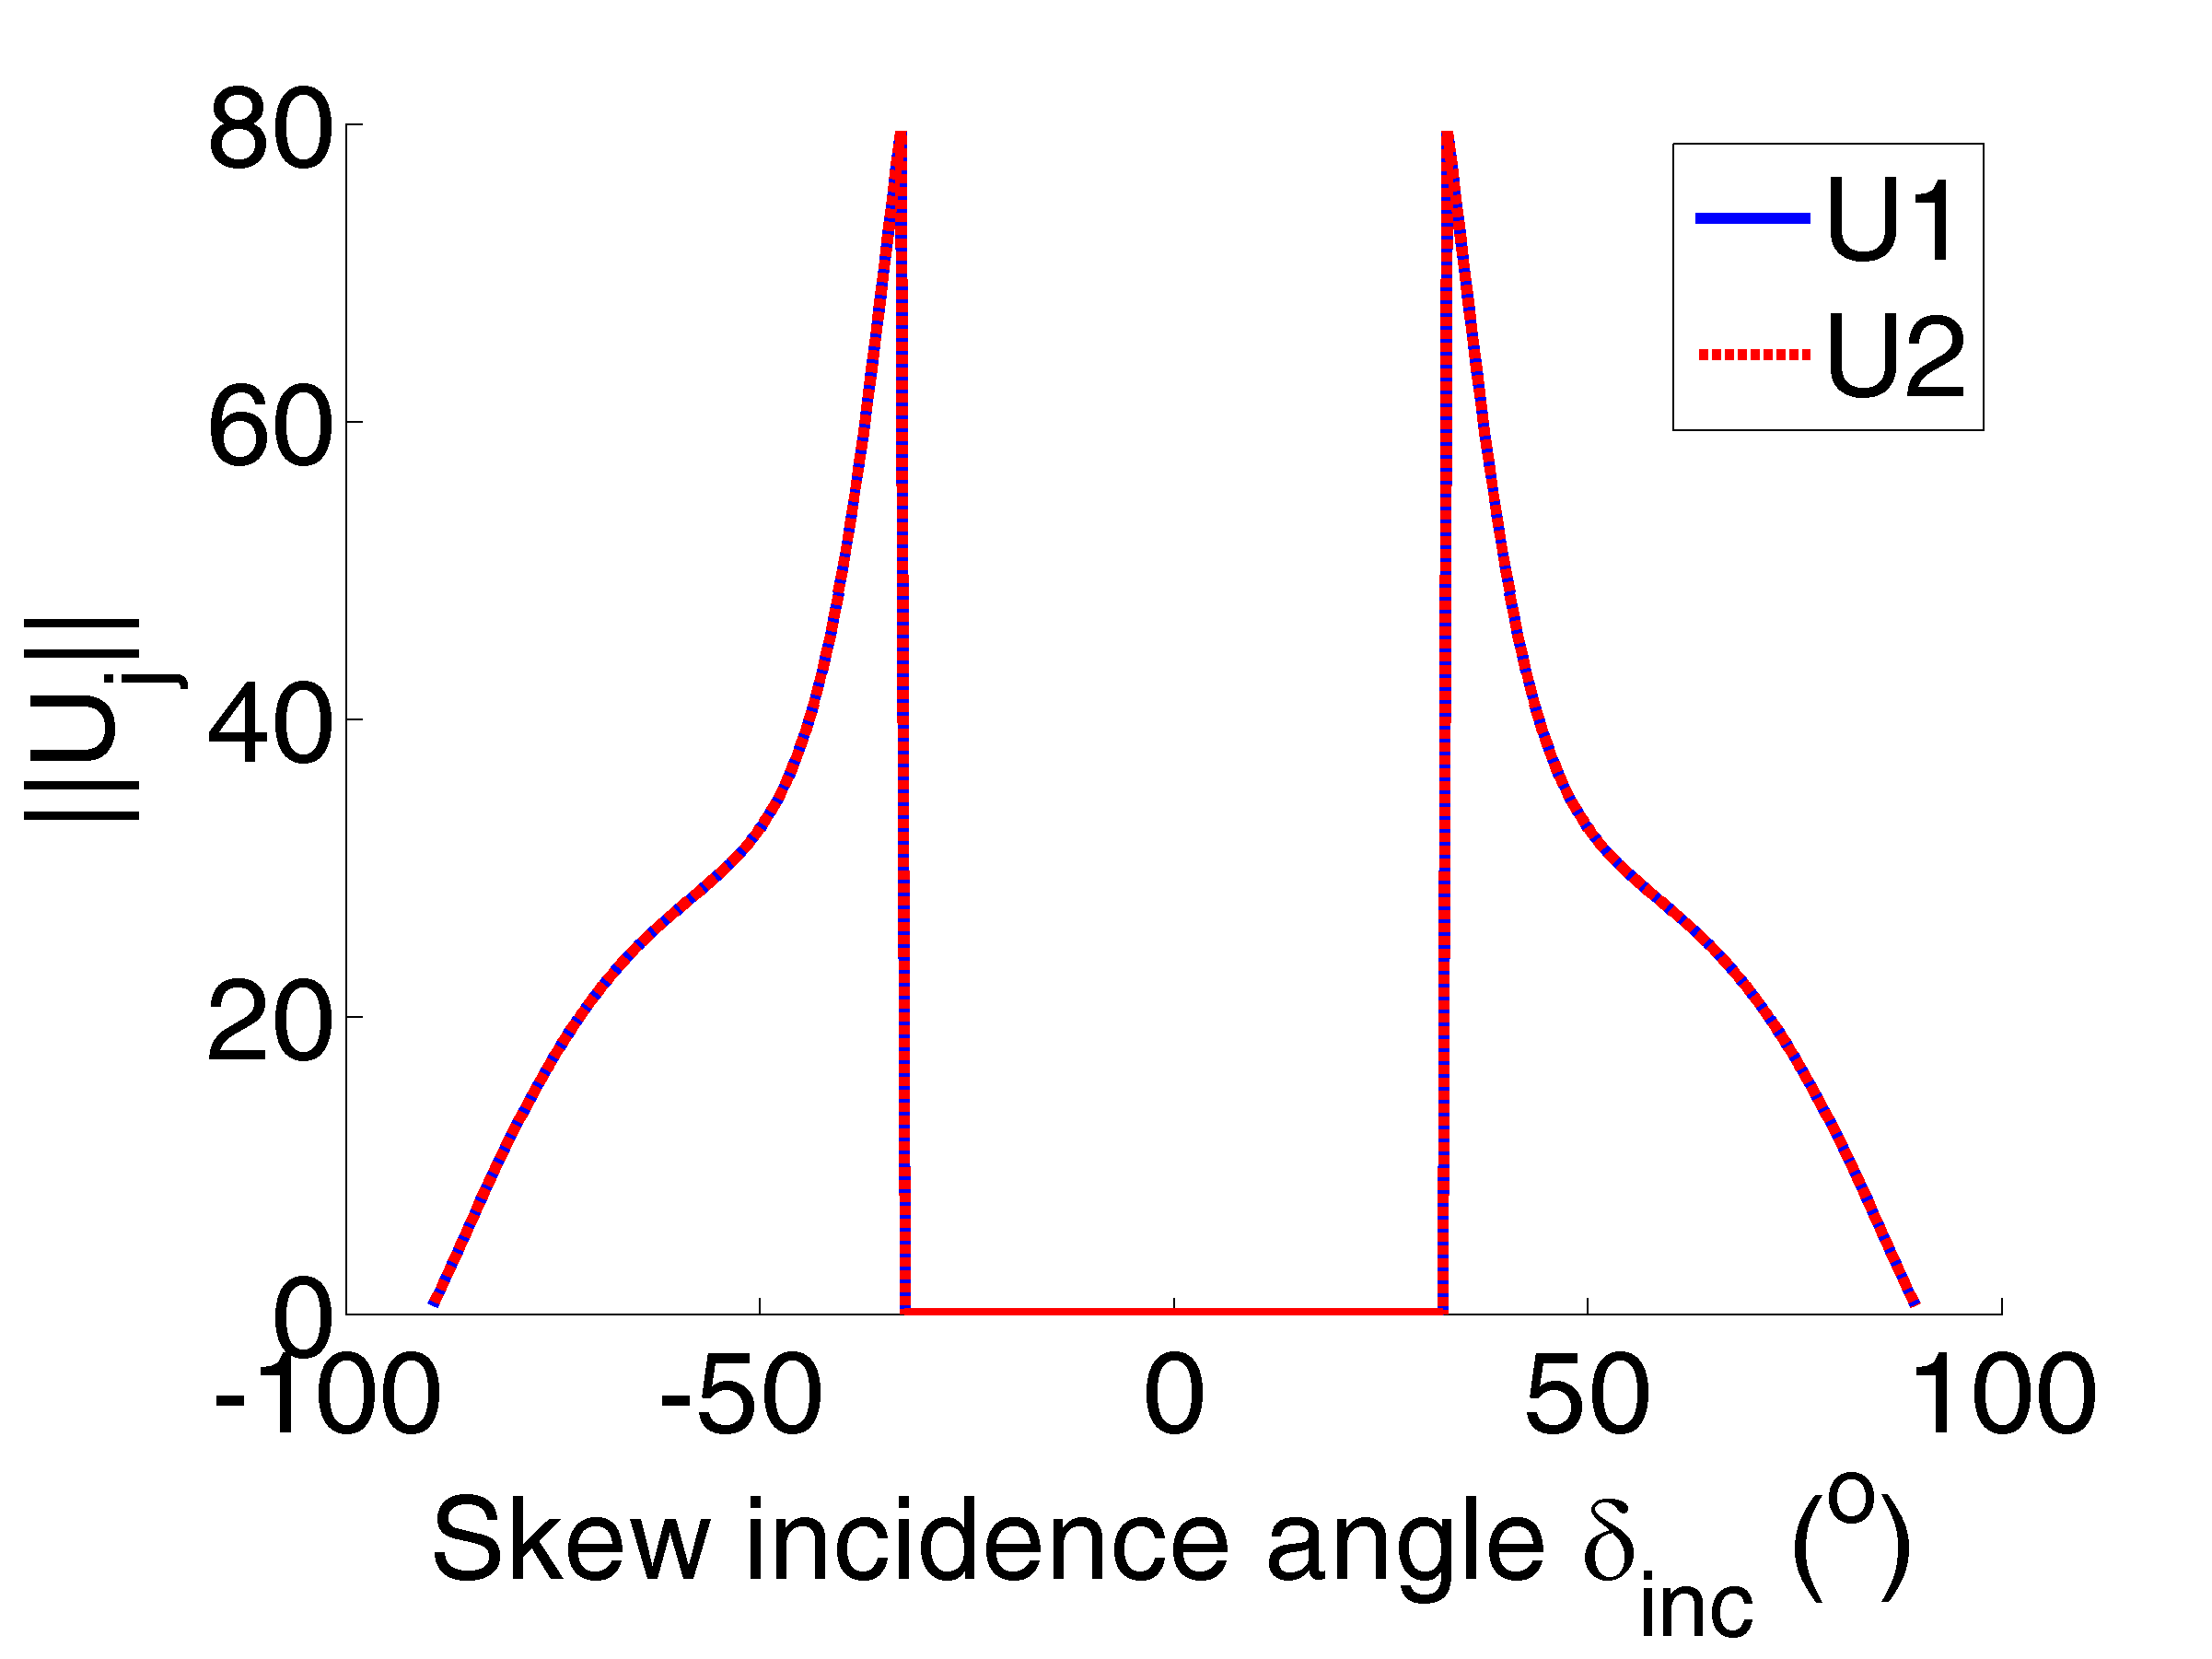
\includegraphics[width=\textwidth]{images/chapter4/Resultats_3D/U1TH_180_50.png}
        \caption{Incident TH wave}
        \label{Resultat_3D:U1TH}
    \end{subfigure}
   \begin{subfigure}[b]{0.32\textwidth}
        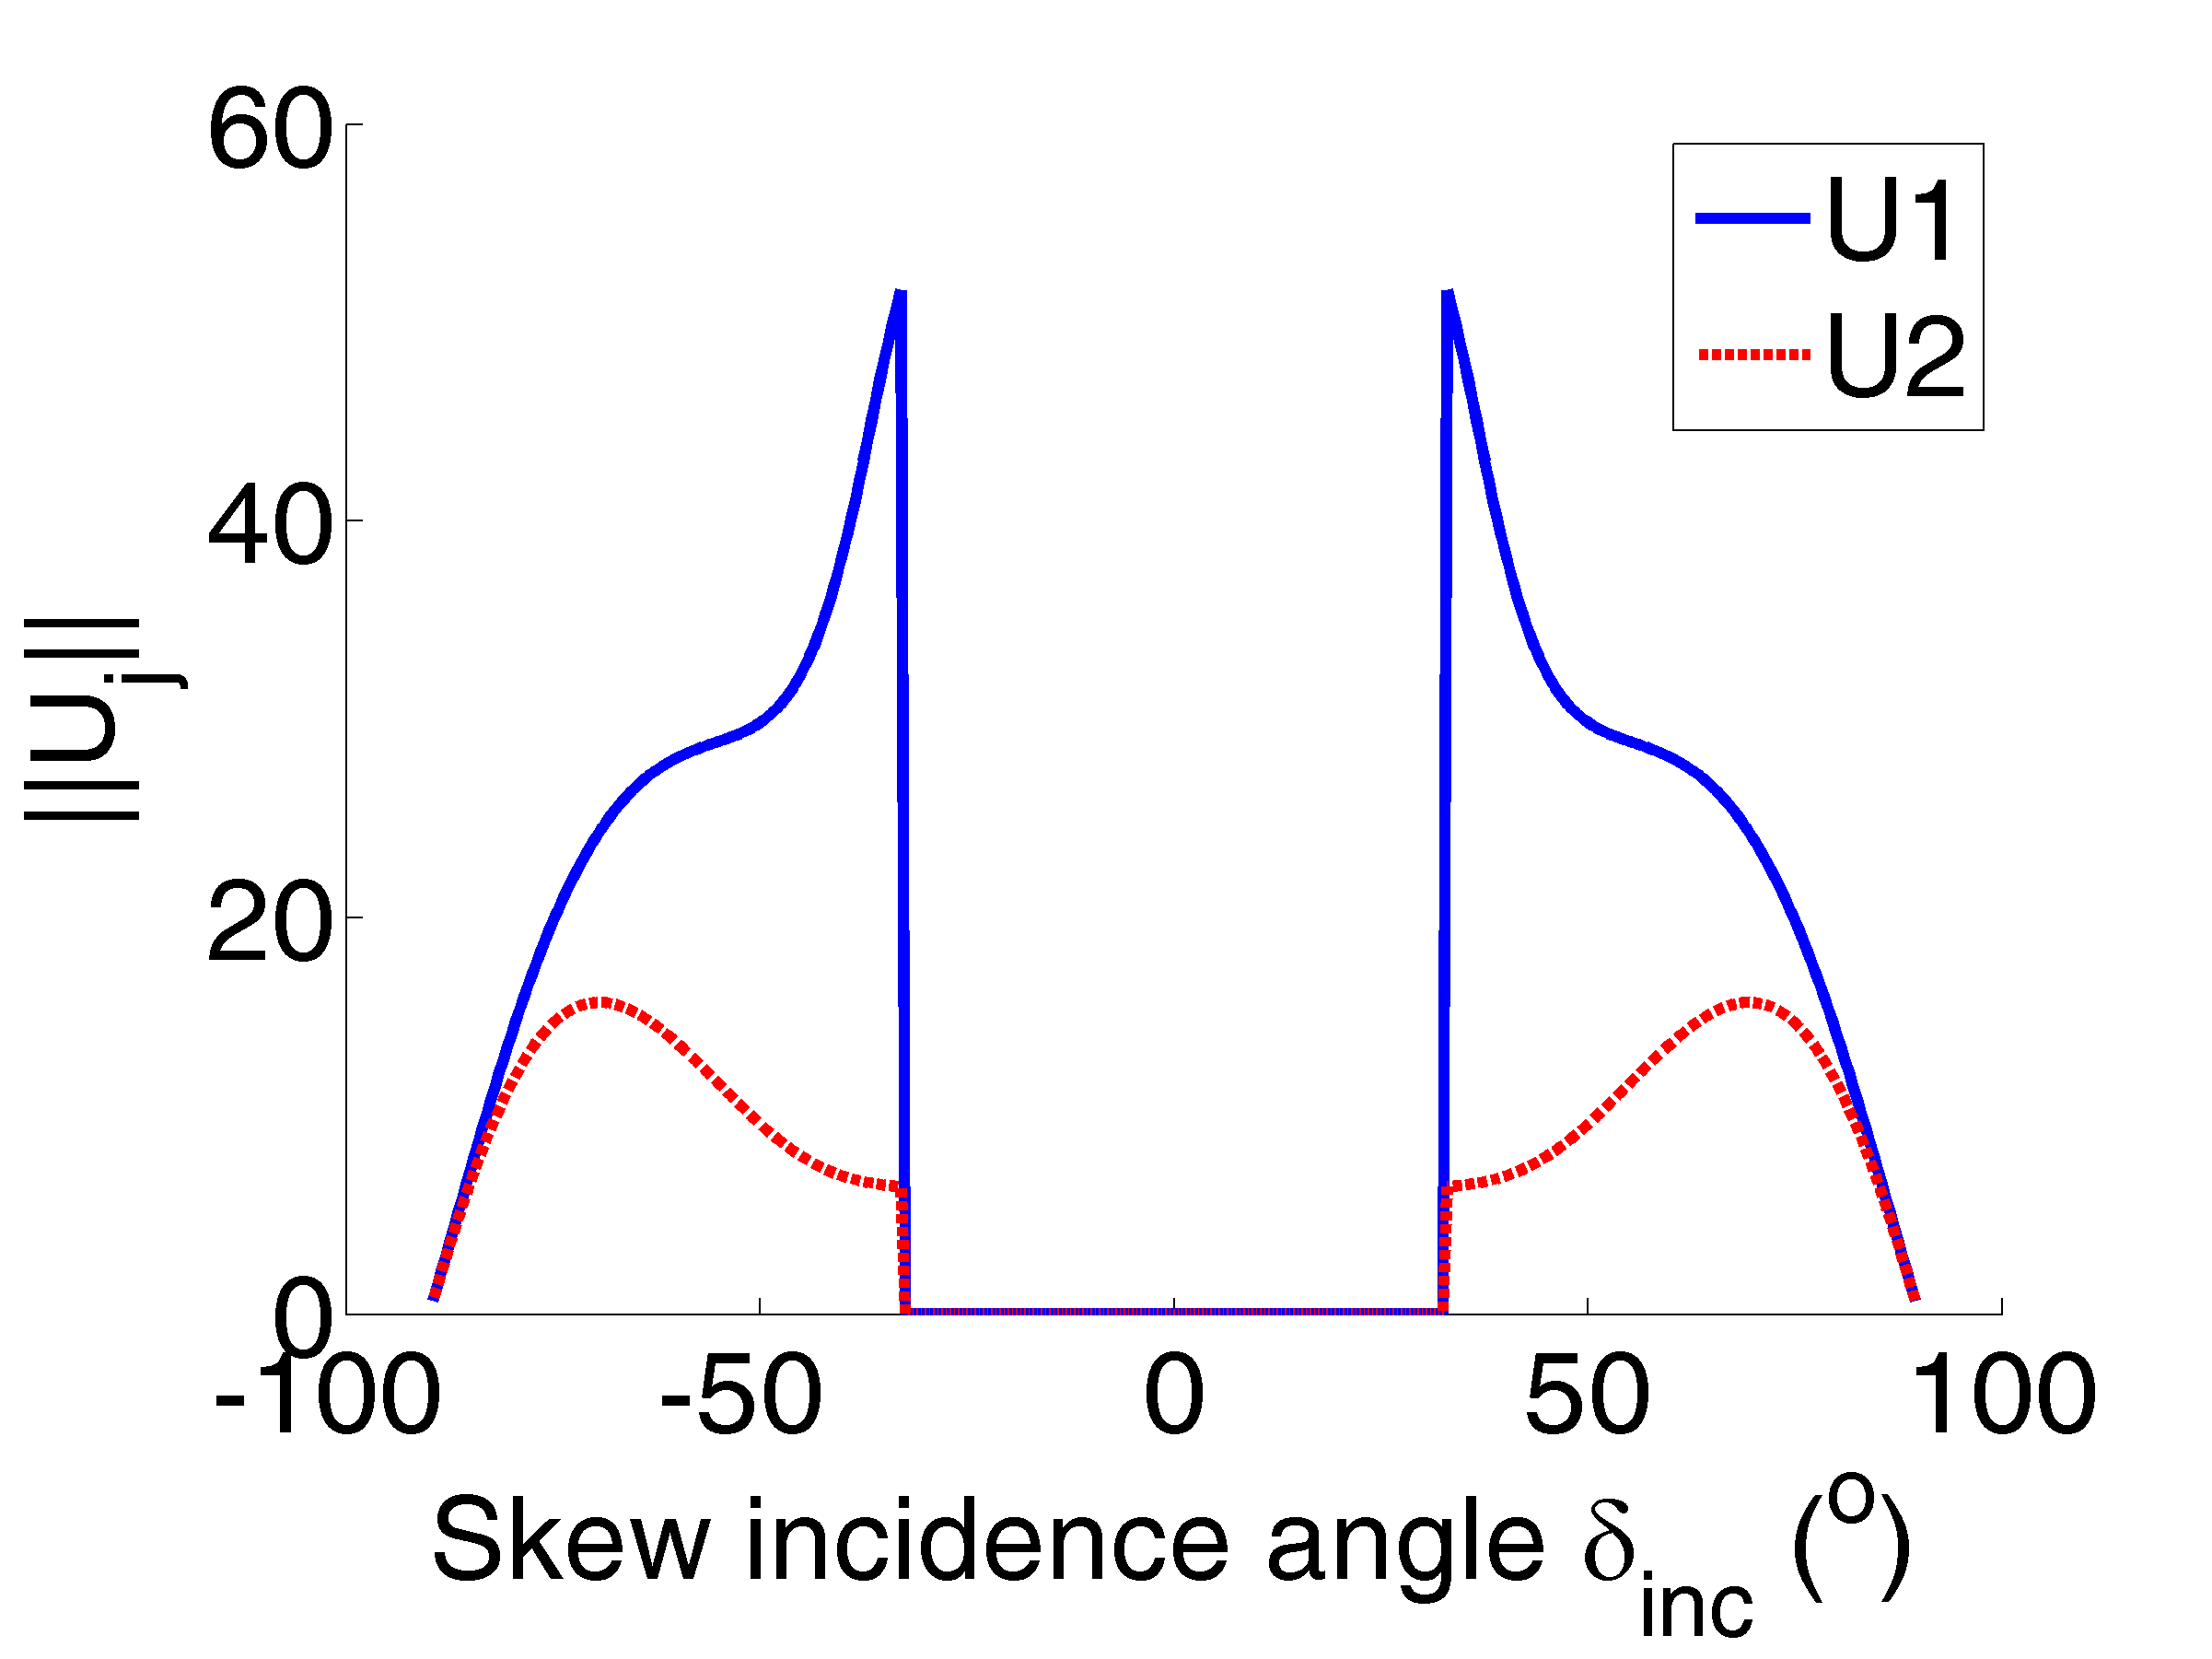
\includegraphics[width=\textwidth]{images/chapter4/Resultats_3D/U1TV_180_50.png}
        \caption{Incident TV wave}
        \label{Resultat_3D:U1TV}
    \end{subfigure} 
\caption{$||\mathbb{U}_j||, \, \, j=1,2$ for $\varphi=180^o$ and $\theta_{inc}=50^o$}
\label{Resultat_3D:U1}
\end{figure}

Fig.~\ref{Resultat_3D:U1} shows $||\mathbb{U}_j||, \, \, j=1,2$ for incident L (see Fig.~\ref{Resultat_3D:U1L}), TH (see Fig.~\ref{Resultat_3D:U1TH}) and TV (see Fig.~\ref{Resultat_3D:U1TV}) waves with an angle $\theta_{inc}=50^o$ on an infinite plane. The thick blue line represents $||\mathbb{U}_1||$ and the dashed red line represents $||\mathbb{U}_2||$. In the case of an incident L wave, as expected, $||\mathbb{U}_1||$ and $||\mathbb{U}_2||$ are very small (of the order of the numerical computation error). For incident T waves, however, when the incident skew angle is higher than the critical angle, $||\mathbb{U}_1||$ and $||\mathbb{U}_2||$ are suddenly very large. Because this is only the case when $\crit$, we beleive that this might be an error in the numerical evaluation, rather than a miscalculation of operators $\mathbb{D}(\cdot,\cdot)$ or $\mathbb{T}(\cdot,\cdot)$, which would have produced errors visible in cases where $\noncr$. 

In any case, when $\crit$, the code developed according to the theory described in this chapter produces diverging results (see for example Fig.~\ref{Resultat_3D:D}). We are not sure what the cause of this error is, and additionnal work is necessary in order to solve this problem.

In the meantime, in order to obtain physically coherent results, the following approximation is applied (only for incident T waves) :
\begin{subequations}
\begin{equation}
\mathbb{D}(\cdot,\cdot)|_{\delta_{\beta}>\delta_C} \approx \mathbb{D}(\cdot,\cdot)|_{\delta_{\beta}=\delta_C-\epsilon}
\end{equation}
\begin{equation}
\mathbb{T}(\cdot,\cdot)|_{\delta_{\beta}>\delta_C} \approx \mathbb{T}(\cdot,\cdot)|_{\delta_{\beta}=\delta_C-\epsilon}
\end{equation}
\label{const_reg_approx}
\end{subequations}

\begin{figure}
\centering
\begin{subfigure}[b]{0.45\textwidth}
        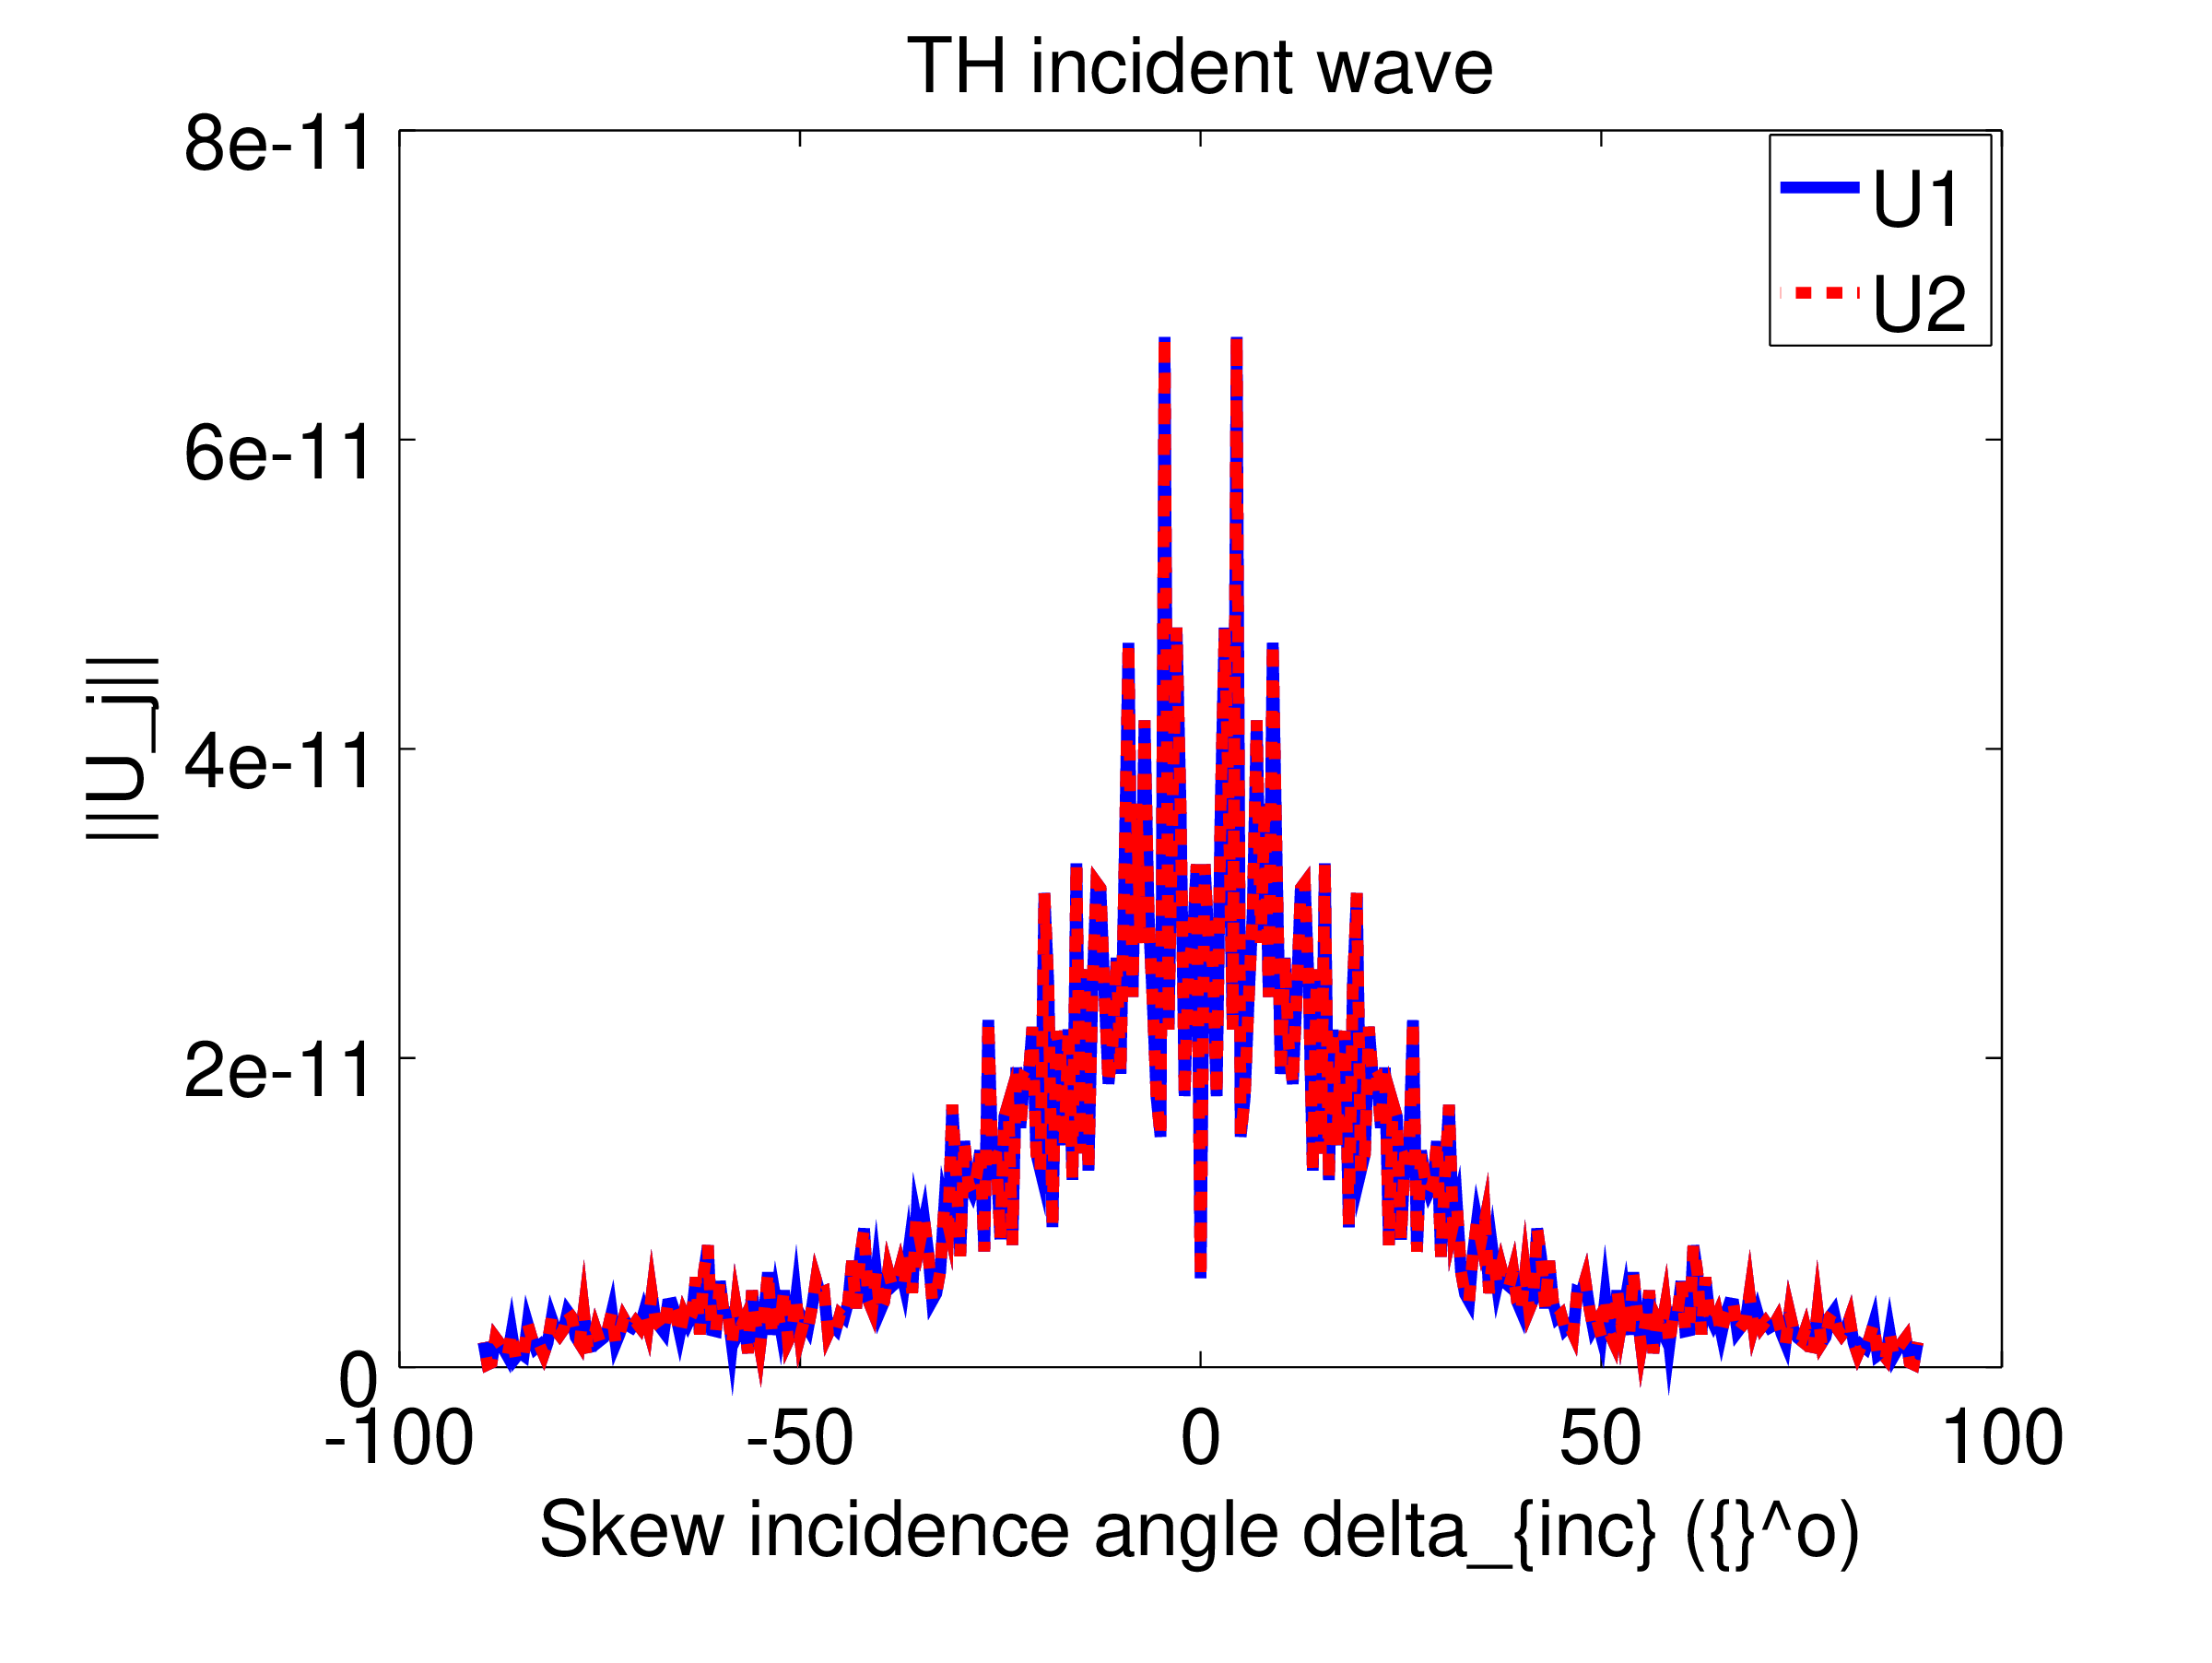
\includegraphics[width=\textwidth]{images/chapter4/const_reg/U1TH_180_50.png}
        \caption{Incident TH wave}
        \label{const_reg:U1TH}
    \end{subfigure}
   \begin{subfigure}[b]{0.45\textwidth}
        \includegraphics[width=\textwidth]{images/chapter4/const_reg/U1TV_180_50.png}
        \caption{Incident TV wave}
        \label{const_reg:U1TV}
    \end{subfigure} 
\caption{$||\mathbb{U}_j||, \, \, j=1,2$ for $\varphi=180^o$ and $\theta_{inc}=50^o$}
\label{const_reg:U1}
\end{figure}

Fig.~\ref{const_reg:U1} shows $||\mathbb{U}_j||, \, \, j=1,2$ obtained with approximations \eqref{const_reg_approx} for incident TH (see Fig.~\ref{const_reg:U1TH}) and TV (see Fig.~\ref{const_reg:U1TV}) waves. with an angle $\theta_{inc}=50^o$ on an infinite plane. The thick blue line represents $||\mathbb{U}_1||$ and the dashed red line represents $||\mathbb{U}_2||$. Using  approximation \eqref{const_reg_approx}, $||\mathbb{U}_1||$ and $||\mathbb{U}_2||$ now behave as expected, even when $\crit$ and are  of the order of the numerical computation error.

In order to illustrate the effect of approximation \eqref{const_reg_approx} in the case where $\crit$, an example is given in the following

\subsection{Numerical approximation in the case $\crit$}

In the previous subsection, it has been made apparent that the regular part of the spectral functions is miscalculated in the case of an incident T wave with a skew angle higher than the critical angle. The cause for this has not yet been found and in the meantime, approximation \eqref{const_reg_approx} has been proposed in order to obtain a non-diverging diffraction coefficient in these cases. In this subsection, we provide an example of the effect of approximation \eqref{const_reg_approx} on the resulting diffraction coefficent. To do so, the L, TH and TV diffraction coefficients are computed using \eqref{C4:Dbeta} for a steel wedge ($c_L=5700m.s^{-1}$ and $c_T=3200m.s^{-1}$) of angle $\varphi=140^o$ illuminated by a TH wave with and angle $\theta_{inc}=70^o$. The spectral functions are evaluated at $\xi=\nuti_{\beta}\cos\theta -i10^{-8}$ (a small negative imaginary part is added to ensure that the recursive equations \eqref{C4:recur} are valid) every $0,5^o$ for $0\leq\theta\leq \varphi$ and for $-90^o\leq \delta_{\alpha} \leq 90^o$.

\begin{figure}
\centering
\begin{subfigure}[b]{0.32\textwidth}
        \includegraphics[width=\textwidth]{images/chapter4/Resultats_3D/XpropL_140_70_TH.png}
        \caption{Diffracted L wave}
        \label{Resultat_3D:DL}
    \end{subfigure}
\begin{subfigure}[b]{0.32\textwidth}
        \includegraphics[width=\textwidth]{images/chapter4/Resultats_3D/XpropTH_140_70_TH.png}
        \caption{Diffracted TH wave}
        \label{Resultat_3D:DTH}
    \end{subfigure}
   \begin{subfigure}[b]{0.32\textwidth}
        \includegraphics[width=\textwidth]{images/chapter4/Resultats_3D/XpropTV_140_70_TH.png}
        \caption{Diffracted TV wave}
        \label{Resultat_3D:DTV}
    \end{subfigure} 
\caption{Absolute value of the diffraction coefficient computed without approximation \eqref{const_reg_approx} for an incident TH wave on a wedge of angle $\varphi=140^o$ with $\theta_{inc}=70^o$}
\label{Resultat_3D:D}
\end{figure}

Fig.~\ref{Resultat_3D:D} shows the absolute value of the diffraction coefficients obtained using the SF code without approximation \eqref{const_reg_approx}. The horizontal axis corresponds to the observation angle $\theta$, the vertical axis corresponds to the incident skew angle $\delta_{\alpha}$ and the magnitude of the diffraction coefficient is represented in color in the $(\theta,\delta_{\alpha})$ plane. Fig.~\ref{Resultat_3D:DL} shows the L diffraction coefficient, Fig.~\ref{Resultat_3D:DTH} shows the TH diffraction coefficient and Fig.~\ref{Resultat_3D:DTV} shows the TV diffraction coefficient. It is clear from these last two figures that the diffraction coefficient abruplty diverges when $\crit$.

\begin{figure}
\centering
\begin{subfigure}[b]{0.45\textwidth}
        \includegraphics[width=\textwidth]{images/chapter4/const_reg/XpropTH_140_70_TH.png}
        \caption{Diffracted TH wave}
        \label{const_reg:DTH}
    \end{subfigure}
   \begin{subfigure}[b]{0.45\textwidth}
        \includegraphics[width=\textwidth]{images/chapter4/const_reg/XpropTV_140_70_TH.png}
        \caption{Diffracted TV wave}
        \label{const_reg:DTV}
    \end{subfigure} 
\caption{Absolute value of the diffraction coefficient computed with approximation \eqref{const_reg_approx} for an incident TH wave on a wedge of angle $\varphi=140^o$ with $\theta_{inc}=70^o$}
\label{const_reg:D}
\end{figure}

Fig.~\ref{const_reg:D} shows the absolute value of the diffraction coefficients obtained using the SF code with approximation \eqref{const_reg_approx}. The horizontal axis corresponds to the observation angle $\theta$, the vertical axis corresponds to the incident skew angle $\delta_{\alpha}$ and the magnitude of the diffraction coefficient is represented in color in the $(\theta,\delta_{\alpha})$ plane. Fig.~\ref{const_reg:DTH} shows the TH diffraction coefficient and Fig.~\ref{const_reg:DTV} shows the TV diffraction coefficient. The diffraction coefficients visible in these two figures are no longer divergent when $\crit$ and their behaviour seems physically coherent. It can be noted that these coefficients seem to diverge when $\delta_{\alpha}$ approaches $\pm90^o$, meaning when the incidence grazes the wedge edge. In this case, the \acrshort{gtd} field diverges because of its proportionality to the factor $(\cos\delta_{\beta})^{-1/2}$, see \eqref{C4:coeffdiff} and another computation method should be considered.

The diffraction coefficients have been computed using the spectral functions method for a steel wedge of angle $\varphi=140^o$ illuminated by an incident TH wave with angle $\theta_{inc}=70^o$ for various incident skew angles. The regular part of the spectral functions, computed according to the method described in \ref{C4:regpart}, diverge when $\crit$. Additional work must be done to find the reason for this instability. In the meantime, a numerical approximation is proposed in order to obtain a diffraction coefficent that only diverges in the directions of specular reflection (as is expected for a \acrshort{gtd} diffraction coefficient). These coefficients have yet to be validated numerically or experimentally.

\section*{Conclusion}
Using the spectral functions method, the elastic wave diffracted by a skew incident plane wave on as stress-free wedge has been studied. In cases where Snell's law of diffraction has a solution for both longitudinal and transversal diffracted waves, a semi-analytical computation method is developed theoretically and numerically. The corresponding code has been tested in three different manners, yielding promising results, but has yet to be validated (numerically or experimentally) for 3D elastic cases. 

In the case of an incident transversal wave, with a skew angle higher than the critical angle in diffraction, Snell's law of diffraction leads only to transversal diffracted waves. This case is also treated theoretically but the corresponding numerical code produces diverging results. Further investigations are necessary in order to solve this problem. In the meantime, an approximate solution is proposed, in order to obtain a less exact, yet physically meaningful result. This approximate solution still remains to be tested.

%
% Chapitre  de conclusion (générale)
%%%%%%%%%%%%%%%%%%%%%%%%%%%%%%%%%%%%%%%%%%%%%%%%%%%%%%%%%%%%%%%%%%%%%%%%%%%%%%%
%\chapter*{Conclusion générale}
\lipsum[26-27]
\section{Une section de conclusion}
\lipsum[28-29]
\subsection{Une sous-section de conclusion}
\lipsum[29-31]
\subsubsection{Une sous-sous-section de conclusion}
\lipsum[31-35]
\paragraph{Un paragraphe de conclusion}
\lipsum[36-38]
\subparagraph{Un sous-paragraphe de conclusion}
\lipsum[39-41]
\subparagraph{Un autre sous-paragraphe de conclusion}
\lipsum[39-41]
\paragraph{Un autre paragraphe de conclusion}
\lipsum[36-38]
\subsubsection{Une autre sous-sous-section de conclusion}
\lipsum[31-37]
\subsection{Une autre sous-section de conclusion}
\lipsum[29-31]
\section{Une autre section de conclusion}
\lipsum[28-43]

%
%%%%%%%%%%%%%%%%%%%%%%%%%%%%%%%%%%%%%%%%%%%%%%%%%%%%%%%%%%%%%%%%%%%%%%%%%%%%%%%
% Début de la partie annexe éventuelle
%%%%%%%%%%%%%%%%%%%%%%%%%%%%%%%%%%%%%%%%%%%%%%%%%%%%%%%%%%%%%%%%%%%%%%%%%%%%%%%
\appendix

\chapter{Steepest Descent Method}
\label{PhaseStationnaire}
The steepest descent method is an integral approximation technique where the integration contour is deformed into a contour $\gamma$ called the steepest descent contour, which passes near a saddle-point of the integrated function. Useful results are stated here without demonstration.

\paragraph{}
The integral to be estimated is of the form :
\begin{equation}
I(\lambda)=\int_{\gamma} f(z)e^{\lambda S(z)}\,dz
\end{equation}
where $\gamma$ is the steepest descent contour, $S$ and $f$ are analytical on all $\mathbb{C}^n$, except for eventually at a finite number of points, and $\lambda>0$. The steepest descent contour $\gamma$ must verify :
\begin{itemize}
\item $C$ and $\gamma$ must have the same endpoints,
\item $\gamma$ passes through at least one saddle point of $g$,
\item Im$(g)$ is constant on $\gamma$.
\end{itemize}

\paragraph{}
Le us denote $\mathbf{S_{xx}}(z)$ the hessian matrix of $S$, defined by :
\begin{equation}
\mathbf{S_{xx}}(z)=\left( \frac{\partial^2 S}{\partial x_i \partial x_j}(z) \right)_{1\leq i,j \leq n},
\end{equation}
then $z_ 0$ is a non-degenerate saddle point of $S$ if and only if :
\begin{eqnarray}
\left\{
\begin{array}{l}
\nabla S(z_0)=0 \\
\mbox{det} \; \mathbf{S_{xx}}(z_0) \neq 0
\end{array}
\right.
\end{eqnarray}

The following proposition is then true :

\begin{prop}
Assume
\begin{description}
  \item[(i)] $f$ and $S$ are holomorphic on an open, bounded and simply connected subset $W_x \subset \mathbb{C}^n$ such that $I_x=W_x \cap \mathbb{R}^n$ is connected,
  \item[(ii)]$ Re\left( S(z) \right)$ has a single maximum reached at exactly one point $z_0 \in I_x$,
  \item[(iii)] $z_0$ is a non-degenerate saddle point of $S$.
\end{description}
The following asymptotic evaluation then holds :
\begin{equation}
I(\lambda) \underset{\lambda \to +\infty}{=} \left( \frac{2\pi}{\lambda} \right)^{n/2} e^{\lambda S(z_0)} \lbrack f(z_0)+ \mathcal{O}(\lambda^{-1}) \rbrack \prod_{j=1}^n (-\mu_j)^{-1/2},
\label{steepformula}
\end{equation}
where $(\mu_j)_{1\leq j \leq n}$ are the eigen values of $\mathbf{S_{xx}}(z_0)$ and their square roots are defined by
$$|\mbox{arg} \sqrt{-\mu_j}| <\frac{\pi}{4} $$
\end{prop}

Note that any if any singularities are crossed during deformation of contour $C$ to contour $\gamma$, their contribution to the integral must be correctly taken into account.

\chapter{Calcul des intégrales $\int_{-1}^1 \frac{\lambda t+ \rho}{Q(t)}\, dt$ et $\int_{-1}^1 \frac{\eta t+ \psi}{P(t)}\, dt$ }
\label{Intégrale}
Avant de nous lancer dans le détail des calculs des coefficients des matrices $\mathbb{D}$ et $\mathbb{T}$, nous allons commencer par calculer deux intégrales élémentaires dont les valeurs seront utilisées dans toute la suite.
\section{Intégrale $\int_{-1}^1 \frac{\lambda t+ \rho}{Q(t)}\, dt$}
\label{calculIntQ}
On calcule :
\begin{equation*}
\int_{-1}^1 \frac{\lambda t+ \rho}{Q(t)}\, dt=\int_{-1}^1 \frac{\lambda t}{iat^2+2\nu t-ia}\,dt+\int_{-1}^1\frac{\rho}{ia(t-q_+)(t-q_-)}\,dt
\end{equation*}
Où on note $q_+,q_-$ les racines de Q. On a:
\begin{equation}
q_\pm=\frac{1}{a}(i\nu\pm\sqrt{a^2-\nu^2})
\label{q1q2}
\end{equation}

\begin{equation*}
\begin{split}
\int_{-1}^1 \frac{\lambda t+ \rho}{Q(t)}\, dt&=\int_{-1}^1 \frac{\frac{\lambda}{2ia} (2iat+2\nu)}{iat^2+2\nu t-ia}\,dt+(\rho-\frac{\lambda \nu}{ia})\int_{-1}^1\frac{1}{ia(t-q_+)(t-q_-)}\,dt\\
&=\frac{\lambda\pi}{2a}+\frac{1}{q_+-q_-}\left(\frac{\rho}{ia}+\frac{\lambda\nu}{a^2}\right)\int_{-1}^1\left(\frac{1}{t-q_+}-\frac{1}{t-q_-}\right)\,dt
\end{split}
\end{equation*}
On réinjecte les expressions de $q_\pm$ données par (\ref{q1q2}):
\begin{equation*}
\begin{split}
\int_{-1}^1 \frac{\lambda t+ \rho}{Q(t)}\, dt&=\frac{\lambda\pi}{2a}+\frac{1}{2\sqrt{a^2-\nu^2}}\left(\frac{\lambda\nu}{a}-i\rho\right)\log\left(\frac{(1-q_+)(1+q_-)}{(1-q_-)(1+q_+)}\right)\\
&=\frac{\lambda\pi}{2a}+\frac{1}{2\sqrt{a^2-\nu^2}}\left(\frac{\lambda\nu}{a}-i\rho\right)\log\left(\frac{-\nu^2-(a-\sqrt{a^2-\nu^2})^2}{-\nu^2-(a+\sqrt{a^2-\nu^2})^2}\right)\\
&=\frac{\lambda\pi}{2a}+\frac{1}{2\sqrt{a^2-\nu^2}}\left(\frac{\lambda\nu}{a}-i\rho\right)\log\left(\frac{-a+\sqrt{a^2-\nu^2}}{-a-\sqrt{a^2-\nu^2}}\right)\\
&=\frac{\lambda\pi}{2a}+\frac{1}{\nu\sqrt{\frac{a^2}{\nu^2}-1}}\left(i\rho-\frac{\lambda\nu}{a}\right)\log\left(\frac{a}{\nu}+\sqrt{\frac{a^2}{\nu^2}-1}\right)
\end{split}
\end{equation*}
Soit finalement :
\begin{equation}
\int_{-1}^1 \frac{\lambda t+ \rho}{Q(t)}\, dt=\frac{\lambda}{\nu}\mbox{sog}(\frac{a}{\nu})+i\frac{\rho}{\nu}\mbox{rog}(\frac{a}{\nu})
\label{intQ}
\end{equation}
On a défini la fonction suivante, pour $a>1$
\begin{equation}
\mbox{rog}(a)=\int_{-1}^1\frac{dx}{a(1-x^2)+2ix}=\frac{1}{\sqrt{a^2-1}}\log(a+\sqrt{a^2-1})
\label{defrog}
\end{equation}
La branche de coupure de la racine carrée est le long de l'axe des réels négatifs. On definit ensuite :
\begin{equation}
\mbox{sog}(a)=\frac{1}{a}\left(\frac{\pi}{2}-\mbox{rog}(a)\right)
\label{defsog}
\end{equation}
\section{Intégrale $\int_{-1}^1 \frac{\eta t+ \psi}{P(t)}\, dt$}
\label{calculintP}
On calcule :
\begin{equation*}
\int_{-1}^1 \frac{\eta t+ \psi}{P(t)}\, dt = \int_{-1}^1 \frac{\eta t}{(\nu\sin\tilde{\varphi}-b)t^2-2i\nu t\cos\tilde{\varphi}+\nu\sin\tilde{\varphi}+b}\,dt +\int_{-1}^1 \frac{\psi}{(\nu\sin\tilde{\varphi}-b)(t-p_+)(t-p_-)}\, dt
\end{equation*}
Où on note $p_+,p_-$ les racines de $P$. On a :
\begin{equation}
p_\pm=\frac{\nu i \cos\tilde{\varphi}\pm \sqrt{b^2-\nu^2}}{\nu\sin\varphi-b}
\label{p1p2}
\end{equation}
\begin{equation*}
\begin{split}
\int_{-1}^1 \frac{\eta t+ \psi}{P(t)}\, dt =& \int_{-1}^1 \frac{\frac{\eta}{2(\nu\sin\tilde{\varphi}-b)}(2(\nu\sin\tilde{\varphi}-b)t-2i\nu\cos\tilde{\varphi})}{(\nu\sin\tilde{\varphi}-b)t^2-2i\nu t\cos\tilde{\varphi}+\nu\sin\tilde{\varphi}+b}\,dt\\
&+(\psi+\frac{\eta i\nu\cos\tilde{\varphi}}{\nu\sin\tilde{\varphi}-b})\int_{-1}^1 \frac{dt}{(\nu\sin\tilde{\varphi}-b)(t-p_+)(t-p_-)}\\
=&\frac{i\eta}{\nu\sin\tilde{\varphi}-b}(\tilde{\varphi}-\frac{\pi}{2})\\
&+\frac{1}{p_+-p_-}\left(\frac{\psi}{\nu\sin\tilde{\varphi}-b}+\frac{\eta i\nu\cos\tilde{\varphi}}{(\nu\sin\tilde{\varphi}-b)^2}\right)\int_{-1}^1 \left(\frac{1}{t-p_+}-\frac{1}{t-p_-}\right)\,dt\\
\end{split}
\end{equation*}
On réinjecte les expressions de $p_\pm$ données par (\ref{p1p2}) :
\begin{equation*}
\begin{split}
\int_{-1}^1 \frac{\eta t+ \psi}{P(t)}\, dt =&\frac{i\eta}{\nu\sin\tilde{\varphi}-b}(\tilde{\varphi}-\frac{\pi}{2})+\frac{1}{2\sqrt{b^2-\nu^2}}\left(\psi+\frac{\eta i\nu\cos\tilde{\varphi}}{\nu\sin\tilde{\varphi}-b}\right)\log\left(\frac{(1-p_+)(1+p_-)}{(1-p_-)(1+p_+)}\right)\\
=&\frac{i\eta}{\nu\sin\tilde{\varphi}-b}(\tilde{\varphi}-\frac{\pi}{2})\\
&+\frac{1}{2\sqrt{b^2-\nu^2}}\left(\psi+\frac{\eta i\nu\cos\tilde{\varphi}}{\nu\sin\tilde{\varphi}-b}\right)\log\left(\frac{-\nu^2\cos^2\tilde{\varphi}-(\nu\sin\tilde{\varphi}-b-\sqrt{b^2-\nu^2})^2}{-\nu^2\cos^2\tilde{\varphi}-(\nu\sin\tilde{\varphi}-b+\sqrt{b^2-\nu^2})^2}\right)\\
=&\frac{i\eta}{\nu\sin\tilde{\varphi}-b}(\tilde{\varphi}-\frac{\pi}{2})+\frac{1}{2\sqrt{b^2-\nu^2}}\left(\psi+\frac{\eta i\nu\cos\tilde{\varphi}}{\nu\sin\tilde{\varphi}-b}\right)\log\left(\frac{b+\sqrt{b^2-\nu^2}}{b-\sqrt{b^2-\nu^2}}\right)\\
=&\frac{i\eta}{\nu\sin\tilde{\varphi}-b}(\tilde{\varphi}-\frac{\pi}{2})+\frac{1}{\nu\sqrt{\frac{b^2}{\nu^2}-1}}\left(\psi+\frac{\eta i\nu\cos\tilde{\varphi}}{\nu\sin\tilde{\varphi}-b}\right)\log\left(\frac{b}{\nu}+\sqrt{\frac{b^2}{\nu^2}-1}\right)
\end{split}
\end{equation*}
Finalement :
\begin{equation}
\int_{-1}^1 \frac{\eta t+ \psi}{P(t)}\, dt =\frac{i\eta}{\nu\sin\tilde{\varphi}-b}\lbrack\tilde{\varphi}-\frac{\pi}{2}+\cos\tilde{\varphi} \mbox{rog}(\frac{b}{\nu})\rbrack+\frac{\psi}{\nu}\mbox{rog}(\frac{b}{\nu})
\label{intP}
\end{equation}

\chapter{Computation details for the coefficients of matrix $\mathbb{D}(a,b)$}
\label{matD}
In each chapter of this manuscript, a matrix $\mathbb{D}$ appears, the coefficients of which must be determined analytically. These coefficients are linear combinations of integrals noted $I_1^*$ to $I_5^*$. In this appendix, these integrals are defined and the details of their computation is given. Finally, expressions of the coefficients of matrix $\mathbb{D}$ in the acoustic case and 2D and 3D elastic cases are given, with respect to integrals $I_1^*$ to $I_5^*$. In all the following, $\nuti \in \{ 1,\nu_T,\nuti_L,\nuti_T \}$.

\section{Integral $I_1^*$}
\label{calcI1}
Integral $I_1^*$ is defined by :
\begin{equation}
\label{defI1}
I_1^*=\int_{-\infty}^{+\infty} \frac{y}{(y+ib)(y-ia)\sqrt{\nuti^2+y^2}}\,dy
\end{equation}
When $a+b \neq 0$, we have the simple elements decomposition :
\begin{equation}
\frac{y}{(y+ib)(y-ia)}=\frac{1}{a+b} \left( \frac{b}{y+ib}+\frac{a}{y-ia} \right), 
\label{decomp2}
\end{equation}
which leads to
\begin{equation}
I_1^*= \frac{1}{a+b} \left( \int_{-\infty}^{+\infty} \frac{b}{(y+ib)\sqrt{\nuti^2+y^2}} \,dy +\int_{-\infty}^{+\infty} \frac{a}{(y-ia)\sqrt{\nuti^2+y^2}} \,dy \right)
\end{equation}
In each of these integrals, the following variable change is applied :
\begin{equation}
\begin{split}
 y&=2\nuti \frac{t}{1-t^2} \\
\sqrt{\nuti^2+y^2}&=\nuti\left( \frac{1+t^2}{1-t^2} \right)  \\
 dy&= 2\nuti \frac{1+t^2}{(1-t^2)^2}dt 
\end{split}
\label{changevar}
\end{equation}
Yielding
\begin{equation}
\int_{-\infty}^{+\infty} \frac{dy}{(y-ia)\sqrt{\nuti^2+y^2}}=\int_{-1}^1\frac{2\,dt}{2\nuti t-ia(1-t^2)}
\end{equation}
Finally, formula \eqref{intQ} is applied :
\begin{equation}
I_1^*=\frac{2ia}{(a+b)\nuti}\mbox{rog}(a/\nuti)-\frac{2ib}{(a+b)\nuti}\mbox{rog}(b/\nuti)
\label{valI1}
\end{equation}

\section{Integral $I_2^*$}
\label{calcI2}
Integral $I_2^*$ is defined by :
\begin{equation}
I_2^*=  \int_{-\infty}^{+\infty} \frac{y\sqrt{\nuti^2+y^2}}{(y+ib)(y-ia)}\, dy
\label{defI2}
\end{equation}
Note that
\begin{equation*}
\begin{split}
I_2^*&=\nuti^2 \int_{-\infty}^{+\infty}  \frac{y}{(y+ib)(y-ia)\sqrt{\nuti^2+y^2}}\,dy+ \int_{-\infty}^{+\infty} \frac{y^3}{(y+ib)(y-ia)\sqrt{\nuti^2+y^2}} \, dy\\
I_2^*&=\nuti^2 I_1^*+I_3^*,
\end{split}
\end{equation*}
where integrals $I_1^*$ and $I_3^*$ are defined by equations \eqref{defI1} and \eqref{defI3} and their expressions are given by \eqref{valI1} and \eqref{valI3} respectively.

\section{Integral $I_3^*$}
\label{calcI3}
Integral $I_3^*$ is defined by :
\begin{equation}
I_3^*=\int_{-\infty}^{+\infty} \frac{y^3}{(y+ib)(y-ia)\sqrt{\nuti^2+y^2}} \,dy
\label{defI3}
\end{equation}
The simple elements decomposition \eqref{decomp2} leads to
\begin{equation}
I_3^*=\frac{b}{a+b}\int_{-\infty}^{+\infty} \frac{y^2}{(y+ib)\sqrt{\nuti^2+y^2}} \, dy +\frac{a}{a+b}\int_{-\infty}^{+\infty} \frac{y^2}{(y-ia)\sqrt{\nuti^2+y^2}} \, dy
\label{decompI3}
\end{equation}

Once again, variable change \eqref{changevar} is applied
\begin{equation}
 \int_{-\infty}^{+\infty} \frac{y^2}{(y-ia)\sqrt{\nuti^2+y^2}} \,dy = \int_{-1}^1 \frac{8\nuti^2t^2}{(1-t^2)^2(2\nuti t -ia(1-t^2))} \, dt
\end{equation}

The integrated functions can be decomposed as such :
\begin{equation}
\frac{t^2}{(1-t^2)^2(2\nuti t -ia(1-t^2))}=\frac{\alpha}{1-t}+\frac{\beta}{1+t}+ \frac{\gamma}{(1-t)^2}+\frac{\delta}{(1+t)^2} +\frac{\lambda t + \rho }{2\nuti t-ia(1-t^2)},
\label{elemsimpl3}
\end{equation}
where the coefficients $\alpha,\beta,\gamma,\delta,\lambda,\rho$ will be determined in the sequel.

To determine $\gamma$, \eqref{elemsimpl3} is multiplied by $(1-t)^2$ and the result is evaluated at $t=1$. Similarly, $\delta$ is determined by multiplying \eqref{elemsimpl3} by $(1+t)^2$ and evaluating the result at $t=-1$ :
\begin{subequations}
\begin{equation}
\gamma=\frac{1}{8\nuti}
\end{equation}
\begin{equation}
\delta = -\frac{1}{8\nuti}
\end{equation}
\end{subequations}

The remaining terms are
\begin{equation}
\begin{split}
\frac{\alpha}{1-t}+\frac{\beta}{1+t}&+ \frac{\lambda t + \rho }{2\nuti t-ia(1-t^2)}\\  
~\\
&=\frac{t^2}{(1-t^2)^2(2\nuti t -ia(1-t^2))}-\frac{1}{8\nuti(1-t)^2}+\frac{1}{8\nuti(1+t)^2}  \\
~\\
&=\frac{8\nuti t^2-(1+t)^2(2\nuti t-ia(1-t^2))+(1-t)^2(2\nuti t-ia(1-t^2))}{8\nuti(1-t^2)^2(2\nuti_*-ia(1-t^2))}\\
~\\
&=\frac{iat}{2\nuti(1-t^2)(2\nuti t-ia(1-t^2))}
\end{split}
\end{equation}

To determine $\alpha$, \eqref{elemsimpl3} is multiplied by $(1-t)$ and the result is evaluated at $t=1$. Similarly, $\beta$ is determined by multiplying \eqref{elemsimpl3} by $(1+t)$ and evaluating the result at $t=-1$ :
\begin{subequations}
\begin{equation}
\alpha=\frac{ia}{8\nuti^2}
\end{equation}
\begin{equation}
\beta=\frac{ia}{8\nuti^2}
\end{equation}
\end{subequations}

The remaining term is
\begin{equation}
\begin{split}
 \frac{\lambda t + \rho }{2\nuti t-ia(1-t^2)} &=\frac{iat}{2\nuti(1-t^2)(2\nuti-ia(1-t^2))} -\frac{ia}{8\nuti^2(1-t)}-\frac{ia}{8\nuti^2(1+t)} \\
&= \frac{2\nuti iat-ia(2\nuti t-ia(1-t^2))}{4\nuti^2(1-t^2)(2\nuti t-ia(1-t^2))} \\
&=\frac{-a^2}{4\nuti ^2(2\nuti t-ia(1-t^2))}
\end{split}
\end{equation}
The final coefficients can now be determined by a simple identification :
\begin{subequations}
\begin{equation}
\lambda=0
\end{equation}
\begin{equation}
\rho=-\frac{a^2}{4\nuti^2}
\end{equation}
\end{subequations}

Finally, equation \eqref{intQ} can be applied :
\begin{equation}
\int_{-\infty}^{+\infty} \frac{y^2}{(y-ia)\sqrt{\nuti^2+y^2}} \, dy =2ia\log\left(\frac{1+t_{\nuti}}{1-t_{\nuti}}\right)-2i\frac{a^2}{\nuti}\rog{\frac{a}{\nuti}}
\label{y2_D}
\end{equation}
The value of $\int_{-\infty}^{+\infty} \dfrac{y^2}{(y+ib)\sqrt{\nuti^2+y^2}} \, dy $ can be obtained by taking the complex conjugate of  $\int_{-\infty}^{+\infty} \dfrac{y^2}{(y-ia)\sqrt{\nuti^2+y^2}} \, dy $ replacing $a$ with $b$ in the result. The final result can then be obtained using \eqref{decompI3} :
\begin{equation}
\begin{split}
I_3^*&=i(a-b)\int_{-1}^1 \left( \frac{1}{1-t}+\frac{1}{1+t} \right) \, dt+ 2\nuti \int_{-1}^1 \left( \frac{1}{(1-t)^2}-\frac{1}{(1+t)^2} \right) \, dt \\
 &-\frac{2a^3}{a+b}\int_{-1}^1\frac{dt}{2\nuti t-ia(1-t^2)}-\frac{2b^3}{a+b}\int_{-1}^1\frac{dt}{2\nuti t+ib(1-t^2)}\\
 ~\\
 &=2i(a-b)\log\left(\frac{1+t_{\nuti}}{1-t_{\nuti}}\right)-\frac{2ia^3}{\nuti(a+b)}\mbox{rog}(a/\nuti)+\frac{2ib^3}{\nuti(a+b)}\mbox{rog}(b/\nuti) 
\end{split}
\label{valI3}
\end{equation}
Note the appearance of the diverging term $\log\left(\dfrac{1+t_{\nuti}}{1-t_{\nuti}}\right)$. This term will be compensated by another in the final expression of the coefficients of matrix $\mathbb{D}$. In fact, \eqref{changevar} leads to :
\begin{equation}
\frac{2t_{\nuti}}{1-t_{\nuti}^2}=\frac{A}{\nuti} \mbox{ and } A\rightarrow + \infty \mbox{ when } t_{\nuti} \rightarrow 1
\end{equation}
and
\begin{equation}
1-t_{\nuti} =\frac{(1-t_{\nuti})(1+t_{\nuti})}{1+t_{\nuti}} \sim \frac{\nuti}{A}
\end{equation}
so that
\begin{equation}
\ln\left(\frac{1+t_{\nuti_L}}{1-t_{\nuti_L}}\right)- \ln\left(\frac{1+t_{\nuti_T}}{1-t_{\nuti_T}}\right)\sim \ln\left(\frac{\nuti_T}{\nuti_L}\right) 
\label{compensation}
\end{equation}

\section{Integral $I_4^*$}
\label{calcI4}
Integral $I_4^*$ is defined by :
\begin{equation}
I_4^*=\int_{-\infty}^{+\infty} \dfrac{dy}{(y+ib)(y-ia)\sqrt{\nuti^2+y^2}}
\label{defI4}
\end{equation}
For $a+b\neq0$, 
\begin{equation}
    \frac{1}{(y+ib)(y-ia)}=\frac{-i}{a+b}\left( \frac{1}{y-ia}-\frac{1}{y+ib}\right)
    \label{decomp1}
\end{equation}
Substituting the above decomposition in \eqref{defI4}, we get
\begin{equation}
I_4^*=\frac{i}{a+b} \int_{-\infty}^{+\infty} \left(\frac{1}{(y+ib)\sqrt{\nuti^2+y^2}}-\frac{1}{(y-ia)\sqrt{\nuti^2+y^2}} \right)\,dy
\end{equation}
These integrals have been computed in section \ref{calculIntQ}. Using \eqref{intQ}, we get :
\begin{equation}
I_4^*=\frac{2}{\nuti(a+b)}\left(\rog{a/\nuti}+\rog{b/\nuti} \right)
\label{valI4}
\end{equation}

\section{Integral $I_5^*$}
\label{calcI5}

Integral $I_5^*$ is defined by :
\begin{equation}
I_5^*=\int_{-\infty}^{+\infty} \frac{y^2}{(y+ib)(y-ia)\sqrt{\nuti^2+y^2}}\,dy
\label{defI5}
\end{equation}
Using decomposition \eqref{decomp1} we get
\begin{equation}
I_5^*=\frac{i}{a+b}\int_{-\infty}^{+\infty}\left( \frac{y^2}{(y+ib)\sqrt{\nuti^2+y^2}}-\frac{y^2}{(y-ia)\sqrt{\nuti^2+y^2}}\right)\,dy
\end{equation}
These integrals have been computed at section \ref{calcI3}. Applying formula \eqref{y2_D}, we get :
% En appliquant le changement de variables \eqref{changevar}, on a
% $$\int_{-\infty}^{+\infty}\frac{y}{(y-ia)\sqrt{\nuti_*^2+y^2}} \, dy=\int_{-1}^1 \frac{4\nuti t}{(1-t^2)(2\nuti t-ia(1-t^2))}\,dt$$
% On cherche la décomposition en éléments simples de l'intégrande :
% $$\frac{2\nuti t}{(1-t^2)(2\nuti t-ia(1-t^2)} = \frac{\alpha}{1-t}+\frac{\beta}{1+t}+\frac{\lambda t+\rho}{Q(t)}$$
% On a alors
% $$\alpha=\beta=1$$
% et 
% $$\lambda=0, \, \, \; \rho=2ia$$
% La formule \eqref{intQ} nous donne finalement :
\begin{equation}
I_5^*=2\log\left(\frac{1+t_{\nuti}}{1-t_{\nuti}}\right)-\frac{2}{\nuti(a+b)}\lbrack b^2\rog{b/\nuti}+a^2\rog{a/\nuti}\rbrack
\label{valI5}
\end{equation}

\section{Integral $I_6^*$}
\label{calcI6}
Integral $I_6^*$ is defined by :
\begin{equation}
I_6^*=\int_{-\infty}^{+\infty}\frac{\sqrt{\nuti_*^2+y^2}}{(y-ia)(y+ib)}\,dy
\label{defI6}
\end{equation}
Note that
\begin{equation}
I_6^*=\nuti^2_* I_4^*+I_5^*
\end{equation}
where integrals $I_4^*$ and $I_5^*$ are defined by equations \eqref{defI4} and \eqref{defI5} and their expressions are given by \eqref{valI4} and \eqref{valI5}.

\section{Continuation and conclusion of the computation of the coefficients of $\mathbb{D}(a,b)$}
\label{fincalculsD}
The final steps of the computation of the coefficients of matrices $\mathbb{D}_{lk}$ are given here. For each physical configuration presented in this manuscript, the coefficients can be expressed as linear combinations of integrals $I_1^*$ to $I_5^*$. These combinations are given case by case in the following.

\subsection{Acoustic case}
\label{finalDac}
In the second chapter of this manuscript, which deals with the diffraction of an acoustic wave, the expression of operator $\mathcal{D}(a,b)$ depends on whether the wedge is soft (Dirichlet boundary conditions) or hard (Neumann boundary conditions). Let us begin with the case of a soft wedge.  
\subsubsection{Dirichlet boundary conditions}
\label{finalDacDir}
In the case of Dirichlet boundary conditions, the expression of function $\mathcal{D}(a,b)$ is obtained by substituting \eqref{dmDir} in \eqref{ldbis} for $a>1$ and $b>1$ :
\begin{equation}
\mathcal{D}(a,b) = \int_{-\infty}^{+\infty} \dfrac{1}{ y+ib} \, \dfrac{1}{y -i a} \,\dfrac{1}{\zeta_0^0(iy)} \, dy . 
\end{equation}
According to \eqref{zeta_function}, the above expression can be simplified using the relation
\begin{equation}
\zeta_0^0(iy)= - \sqrt{1+y^2}.
\label{Appendix:zeta0iy}
\end{equation}
By setting $\nuti=1$ in \eqref{defI4}, we find :
\begin{equation}
\mathcal{T}(a,b)=-I_4^1
\end{equation}
This integral is computed in section \ref{calcI4} and its value is given by \eqref{valI4}.
\subsubsection{Neumann boundary conditions}
\label{finalDacNeu}
In the case of Neumann boundary conditions, the expression of function $\mathcal{D}(a,b)$ is obtained by substituting \eqref{dmNeu} in \eqref{ldbis} for $a>1$ and $b>1$ :
\begin{equation}
\mathcal{D}(a,b) = \int_{-\infty}^{+\infty} \dfrac{dy}{ (y+ib)(y-ia)} \, dy .
\end{equation}
The result can be computed directly, by using Cauchy's residue theorem, yielding :
\begin{equation}
\mathcal{D}(a,b)=\dfrac{2\pi}{a+b}
\end{equation}

\subsection{2D elastic case}
In the third chapter of this manuscript, which deals with the 2D diffraction of an elastic wave, the coefficients of matrix $\mathbb{D}(a,b)$ are linear combinations of integrals $I_1^*$ to $I_3^*$. These linear combinations are given in the sequel. In all that follows, $\nuti=1$ when $*=L$ and $\nuti=\nu_T$ when $*=T$.
\label{finalD2D}
The first coefficient can be computed using Gauss' integral formula :
\begin{equation}
\mathcal{D}_1(a,b)=\int_{-\infty}^{+\infty} \frac{dy}{(y+ib)(y-ia)}=\frac{2\pi}{a+b}
\end{equation}
The two other coefficients are linear combinations of $I_1^*$ to $I_3^*$ :
\begin{equation}
\mathcal{D}_2(a,b)=\int_{-\infty}^{+\infty} \frac{-iy(1-2\mu \zeta_L(iy) \zeta_T(iy)+2\mu y^2)}{(y+ib)(y-ia)\zeta_T(iy)} \,dy =i I_1^T-2i\mu(I_2^L-I_3^T)
\label{D2}
\end{equation}
and
\begin{equation}
\mathcal{D}_3(a,b)=\int_{-\infty}^{+\infty} \frac{iy(1-2\mu \zeta_L(iy) \zeta_T(iy)+2\mu y^2)}{(y+ib)(y-ia)\zeta_L(iy)} \,dy=-iI_1^L+2i\mu(I_2^T-I_3^L)
\label{D3}
\end{equation}
This concludes computation of matrix coefficients $\mathbb{D}_{lk}$ for the 2D elastic case.

\subsection{3D elastic case}
\label{finalD3D}
In the fourth chapter of this manuscript, which deals with the 3D diffraction of an elastic wave, the coefficients of matrix $\mathbb{D}(a,b)$ are linear combinations of integrals $I_1^*$ and $I_6^*$. These linear combinations are given in the sequel. In all that follows, $\nuti=\nuti_L$ when $*=L$ and $\nuti=\nuti_T$ when $*=T$.

The first coefficient can be computed using Gauss' integral formula :
\begin{equation}
\mathcal{D}_1(a,b)=\int_{-\infty}^{+\infty} \frac{dy}{(y+ib)(y-ia)}=\frac{2\pi}{a+b}
\end{equation}
The other coefficients are linear combinations of $I_1^*$ to $I_6^*$ :
\begin{equation}
\begin{split}
\mathcal{D}_2^L(a,b)&=\int_{-\infty}^{+\infty} \frac{iy\lbrack 1-2\mu (\zeta_L(iy) \zeta_T(iy)- y^2+\tau^2)\rbrack}{(y+ib)(y-ia)\zeta_L(iy)} \,dy \\
&=-i(1-2\mu\tau^2)I_1^L+2i\mu(I_2^T-I_3^L)
\end{split}
\end{equation}
\begin{equation}
\begin{split}
\mathcal{D}_2^T(a,b)&=\int_{-\infty}^{+\infty} \frac{iy\lbrack 1-2\mu (\zeta_L(iy) \zeta_T(iy)- y^2+\tau^2)\rbrack}{(y+ib)(y-ia)\zeta_T(iy)} \,dy \\
&=-i(1-2\mu\tau^2)I_1^T+2i\mu(I_2^L-I_3^T)
\end{split}
\end{equation}
\begin{equation}
\begin{split}
\mathcal{D}_3^L(a,b)&=\tau\int_{-\infty}^{+\infty} \frac{1-2\mu(\zeta_L(iy)\zeta_T(iy)-y^2+\tau^2)}{(y+ib)(y-ia)\zeta_L(iy)}\,dy \\
&=-\tau(1-2\mu\tau^2)I_4^L-2\mu\tau I_5^L+2\mu\tau I_6^T
\end{split}
\end{equation}
\begin{equation}
\begin{split}
\mathcal{D}_3^T(a,b)&=\tau\int_{-\infty}^{+\infty} \frac{1-2\mu(\zeta_L(iy)\zeta_T(iy)-y^2+\tau^2)}{(y+ib)(y-ia)\zeta_T(iy)}\,dy \\
&=-\tau(1-2\mu\tau^2)I_4^T-2\mu\tau I_5^T+2\mu\tau I_6^L
\end{split}
\end{equation}
This concludes computation of matrix coefficients $\mathbb{D}_{lk}$ for the 3D elastic case.

\chapter{Computation details for the coefficients of matrix $\mathbb{T}(a,b)$}
\label{matT}
Lors des caluls des coefficients de $\mathbb{T}(a,b)$ nous aurons besoin d'un certain nombre de résultats intermédiaires. Nous allons donc commencer par déterminer ceux-ci avant de procéder au calcul final.

\section{Calcul de l'intégrale $J_2^*$}
\label{calculJ2}
On définit :
\begin{equation}
J_2 =\int_{-\infty}^{+\infty} \frac{y^2}{(y-ia)\lbrack b-iy\cos \tilde{\varphi}+ \sqrt{\nuti^2+y^2} \sin \tilde{\varphi}) \rbrack} \, dy
\label{defJ2}
\end{equation}
On effectue une fois de plus le changement de variables (\ref{changevar}) et on obtient désormais :
$$J_2=8\nuti^3 \int_{-1}^1 \frac{t^2(t^2+1)}{(1-t^2)^2\lbrack b(1-t^2)-2\nuti it\cos\tilde{\varphi}+ \sin \tilde{\varphi} \nuti(1+t^2)\rbrack(2\nuti t-ia(1-t^2))}\, dt$$
On cherche la décomposition en éléments simples de l'intégrande :
$$\frac{t^2(1+t^2)}{(1-t)^2(1+t)^2P(t)Q(t)}=\frac{\alpha_2}{1-t}+\frac{\beta_2}{1+t}+\frac{\gamma_2}{(1-t)^2}+\frac{\delta_2}{(1+t)^2}+\frac{\eta_2 t+\psi_2}{P(t)}+\frac{\lambda_2 t +\rho_2}{Q(t)}$$
Où on a défini :
\begin{equation}
P(t)=b(1-t^2)-2\nuti i t\cos\tilde{\varphi}+\nuti\sin\tilde{\varphi}(1+t^2)
\end{equation}
On a donc, pour commencer :
$$ \gamma_2=\frac{e^{i(\pi/2-\tilde{\varphi})}}{8\nuti^2}$$
$$\delta_2=\frac{e^{i(\pi/2+\tilde{\varphi})}}{8\nuti^2}$$
D'où :
\begin{equation*}
\begin{split}
\frac{\alpha_2}{1-t}&+\frac{\beta_2}{1+t} +\frac{\eta_2 t+\psi_2}{P(t)}+\frac{\lambda_2 t +\rho_2}{Q(t)}=\frac{t^2(1+t^2)}{(1-t)^2(1+t)^2P(t)Q(t)}-\frac{e^{i(\pi/2-\tilde{\varphi})}}{8\nuti^2(1-t)^2}-\frac{e^{i(\pi/2+\tilde{\varphi})}}{8\nuti^2(1+t)^2}\\
&=\frac{2iab\sin\tilde{\varphi}t-\nuti^2i\sin(2\tilde{\varphi})t-ab\cos\tilde{\varphi}(1+t^2)}{4\nuti^2 P(t)Q(t)}\\ &+\frac{(2t\sin\tilde{\varphi}+(1+t^2)i\cos\varphi)(2a\cos\tilde{\varphi}t+ai\sin\tilde{\varphi}(1+t^2)-2bt)}{4\nuti(1-t^2) P(t)Q(t)}
\end{split}
\end{equation*}


On a maintenant :
$$\alpha_2=\frac{be^{-2i\tilde{\varphi}}-ae^{-i\tilde{\varphi}}}{8\nuti^3}$$
$$\beta_2=\frac{ae^{i\tilde{\varphi}}-be^{2i\tilde{\varphi}}}{8\nuti^3}$$
Ce qui donne :
\begin{equation}
\begin{split}
\frac{\eta_2 t+\psi_2}{P(t)}+&\frac{\lambda_2 t +\rho_2}{Q(t)}
=\frac{2iab\sin\tilde{\varphi}t-i\nuti^2\sin(2\tilde{\varphi})t-ab\cos\tilde{\varphi}(1+t^2)}{4\nuti^2P(t)Q(t)}\\
&+\frac{1}{4(1-t^2)\nuti^3P(t)Q(t)}\Big( \lbrack 2\nuti^2t\sin\tilde{\varphi}+\nuti^2(1+t^2)i\cos\tilde{\varphi} \rbrack\lbrack2a\cos\tilde{\varphi}t+ai\sin\tilde{\varphi}(1+t^2)-2bt \rbrack\\
&-(b\cos(2\tilde{\varphi})t-at\cos\tilde{\varphi}-ib\sin(2\tilde{\varphi})+ia\sin\tilde{\varphi})P(t)Q(t)\Big) \\
~\\
=&-\frac{b\cos(2\tilde{\varphi})t-at\cos\tilde{\varphi}-ib\sin(2\tilde{\varphi})+ia\sin\tilde{\varphi}}{4\nuti^3P(t)Q(t)}\lbrack 2\nuti bt-iab(1-t^2)-2a\nuti\cos\tilde{\varphi}t\\
&-a\nuti i\sin\tilde{\varphi}(1+t^2)\rbrack +\frac{1}{4\nuti(1-t^2)P(t)Q(t)}\Big( \lbrack 2t\sin\tilde{\varphi}+(1+t^2)i\cos\tilde{\varphi} \rbrack\lbrack 2a\cos\tilde{\varphi}t\\
&+ai\sin\tilde{\varphi}(1+t^2)-2bt \rbrack- (b\cos(2\tilde{\varphi})t-at\cos\tilde{\varphi}-ib\sin(2\tilde{\varphi})+ia\sin\tilde{\varphi})(2\sin\tilde{\varphi}t(1+t^2)\\
&-4i\cos\tilde{\varphi}t^2) \Big)+\frac{2iab\sin\tilde{\varphi}t-i\nuti^2\sin(2\tilde{\varphi})-ab\cos\tilde{\varphi}(1+t^2)}{4\nuti^2P(t)Q(t)}\\
=&-\frac{b\cos(2\tilde{\varphi})t-at\cos\tilde{\varphi}-ib\sin(2\tilde{\varphi})+ia\sin\tilde{\varphi}}{4\nuti^3P(t)Q(t)}\lbrack 2\nuti bt-iab(1-t^2)-2a\nuti\cos\tilde{\varphi}t\\
&-a\nuti i\sin\tilde{\varphi}(1+t^2)\rbrack+\frac{2iab\sin\tilde{\varphi}t-i\nuti^2\sin(2\tilde{\varphi})t-ab\cos\tilde{\varphi}(1+t^2)}{4\nuti^2P(t)Q(t)}\\
&+\frac{2ia\cos^2\tilde{\varphi}t-a\cos\tilde{\varphi}\sin\tilde{\varphi}(1+t^2)+2b\sin\tilde{\varphi}\cos(2\tilde{\varphi})t^2-2ib\cos\tilde{\varphi}\cos(2\tilde{\varphi})t}{4\nuti P(t)Q(t)}
\end{split}
\label{N2}
\end{equation}
Il ne reste plus qu'à déterminer les constantes $\eta_2,\psi_2,\lambda_2,\rho_2$ pour achever le calcul de la décomposition en élements simples. Pour celà, on utilise les considérations générales suivantes :
\paragraph{}
On note $N(t)$ un polynôme de degré 3 et on suppose que l'on a :
\begin{equation}
\frac{\eta t+\psi}{P(t)}+\frac{\lambda t+\rho}{Q(t)}=\frac{N(t)}{P(t)Q(t)}
\label{nsurpq}
\end{equation}
On a défini $p_\pm$ en (\ref{p1p2}) et $q_\pm$ en (\ref{q1q2})
Prenons l'égalité (\ref{nsurpq}) et multiplions la par $P(t)$. En évaluant le résultat en $p_+$ puis en $p_-$, on obtient le système suivant :
\begin{eqnarray*}
\left\{
\begin{array}{l}
\eta p_+ +\psi=\frac{N(p_+)}{Q(p_+)}\\
\eta p_- +\psi=\frac{N(p_-)}{Q(p_-)}
\end{array}
\right.
\end{eqnarray*}
La résolution de ce système donne:
\begin{eqnarray}
\left\{
\begin{array}{l}
\eta=\frac{1}{p_+-p_-}\left[ \frac{N(p_+)}{Q(p_+)}-\frac{N(p_-)}{Q(p_-)} \right] \\
\psi=\frac{N(p_+)}{Q(p_+)}-\eta p_+
\end{array}
\right.
\label{etapsi}
\end{eqnarray}
Par symétrie des rôles de P et Q, on a :
\begin{eqnarray}
\left\{
\begin{array}{l}
\lambda=\frac{1}{q_+-q_-}\left[ \frac{N(q_+)}{P(q_+)}-\frac{N(q_-)}{P(q_-)} \right] \\
\rho=\frac{N(q_+)}{P(q_+)}-\lambda q_+
\end{array}
\right.
\label{lambdarho}
\end{eqnarray}
Dans le cas présent, le numérateur est donné par (\ref{N2}). Les derniers coefficients de la décomposition s'en déduisent donc en utilisant (\ref{etapsi}) et (\ref{lambdarho}).

\paragraph{}
On utilise les formules (\ref{intQ}) et (\ref{intP}) :
\begin{equation}
\begin{split}
J_2\sim &2i\cos\tilde{\varphi} A+2i(a\sin\tilde{\varphi}-b\sin(2\tilde{\varphi}))\ln\left(\frac{1+t_{\nuti}}{1-t_{\nuti}} \right) \\
&+\frac{8i\eta_2\nuti^2}{b/\nuti-\sin\tilde{\varphi}}\left(\frac{\pi}{2}-\tilde{\varphi}-\cos\phiti\,\mbox{rog}(\frac{b}{\nuti}) \right)+8\nuti^2\psi_2 \mbox{rog}(\frac{b}{\nuti} )\\
&+8\nuti^2 \left(\lambda_2 \mbox{sog}(a/\nuti)+i\rho_2 \mbox{rog}(a/\nuti) \right)
\end{split}
\label{valJ2}
\end{equation}
On note l'apparition de termes divergents dans le résultat. Ceux-ci se compenseront lors de la sommation des termes issus des coefficients $\mathcal{T}^T$ avec les termes issus des coefficients $\mathcal{T}^L$. 

\section{Calcul de l'intégrale $J_3^*$}
\label{calculJ3}
On calcule :
\begin{equation}
J_3 = \int_{-\infty}^{+\infty} \frac{1}{(y-ia)\lbrack b-iy\cos \tilde{\varphi}+  \sqrt{\nuti^2+y^2} \sin \tilde{\varphi} \rbrack} \, dy
\label{defJ3}
\end{equation}
Encore une fois, on applique le changement de variables (\ref{changevar}):
$$J_3= 2\nuti \int_{-1}^1 \frac{1+t^2}{(2\nuti t-ia(1-t^2))(b(1-t^2)-2i\nuti t\cos\tilde{\varphi}+\nuti\sin\tilde{\varphi}(1+t^2))} \, dt$$
La décomposition en éléments simples de l'intégrande donne :
$$\frac{1+t^2}{P(t)Q(t)}=\frac{\eta_3 t+\psi_3}{P(t)}+\frac{\lambda_3 t +\rho_3}{Q(t)}$$
Les coefficients s'obtiennent en utilisant les formules (\ref{etapsi}) et (\ref{lambdarho}).

Soit finalement :
\begin{equation}
\begin{split}
J_3=&\frac{2i\eta_3}{b/\nuti-\sin\tilde{\varphi}}\left(\frac{\pi}{2}-\tilde{\varphi}-\cos\tilde{\varphi} \,\mbox{rog}(\frac{b}{\nuti}) \right)+2\psi_3 \mbox{rog}(\frac{b}{\nuti} )\\
&+2\left(\lambda_3 \mbox{sog}(a/\nuti)+i\rho_3 \mbox{rog}(a/\nuti) \right)
\end{split}
\label{valJ3}
\end{equation}
Cette fois, il n'y a aucun terme divergent. 

\section{Calcul de l'intégrale $J_4^*$}
\label{calculJ4}
On définit maintenant :
\begin{equation}
J_4=\int_{-\infty}^{+\infty}\frac{y^3}{(y-ia)\sqrt{y^2+\nuti^2}(b-iy\cos\tilde{\varphi}+\sqrt{\nuti^2+y^2}\sin\tilde{\varphi})}\,dy
\label{defJ4}
\end{equation}
On effectue une fois de plus le changement de variables (\ref{changevar}).
$$J_4=16\nuti^3 \int_{-1}^1 \frac{t^3}{(2\nuti t-ia(1-t^2))(1-t^2)^2(b(1-t^2)-2i\nuti t\cos\tilde{\varphi}+\nuti(1+t^2)\sin\tilde{\varphi})} \, dt $$
On cherche la décomposition en éléments simples de l'intégrande :
\begin{equation*}
\frac{t^3}{(1-t^2)^2P(t)Q(t)}=\frac{\alpha_4}{1-t}+\frac{\beta_4}{1+t}+\frac{\gamma_4}{(1-t)^2}+\frac{\delta_4}{(1+t)^2}+\frac{\eta_4 t+\psi_4}{P(t)}+\frac{\lambda_4 t +\rho_4}{Q(t)}
\end{equation*}

On a :
$$\gamma_4=\frac{e^{i(\pi/2-\tilde{\varphi})}}{16\nuti^2}$$
$$\delta_4=\frac{e^{i(\tilde{\varphi}-\pi/2)}}{16\nuti^2}$$
On calcule :

\begin{equation*}
\begin{split}
\frac{\alpha_4}{1-t}&+\frac{\beta_4}{1+t}+\frac{\eta_4 t+\psi_4}{P(t)}+\frac{\lambda_4 t +\rho_4}{Q(t)}=\frac{8\nuti^2t^3-\lbrack \sin\tilde{\varphi}(1+t^2)+2i\cos\tilde{\varphi} t \rbrack P(t)Q(t)}{8\nuti^2(1-t^2)^2P(t)Q(t)} \\
~\\
=&\frac{\sin\tilde{\varphi}(1+t^2)+2i\cos\tilde{\varphi} t}{8\nuti^2(1-t^2)P(t)Q(t)}\Big( a\nuti(2\cos\tilde{\varphi}t+i\sin\tilde{\varphi}(1+t^2))-b(2\nuti t-ia(1-t^2))\Big)\\
&+\frac{4t^3-(\sin\tilde{\varphi}(1+t^2)+2i\cos\tilde{\varphi} t)(\sin\tilde{\varphi}t(1+t^2)-2i\cos\tilde{\varphi} t^2)}{4(1-t^2)^2P(t)Q(t)}\\
~\\
=&\frac{2ait^2-b\sin\tilde{\varphi}t(1+t^2)-2ib\cos\tilde{\varphi}t^2}{4\nuti(1-t^2)P(t)Q(t)}+\frac{a\nuti i\sin^2\tilde{\varphi}(1-t^2)+iab\sin\tilde{\varphi}(1+t^2)-2ab\cos\tilde{\varphi}t}{8\nuti^2P(t)Q(t)}\\
&-\frac{\sin^2\tilde{\varphi}.t}{4P(t)Q(t)}
\end{split}
\end{equation*}

D'où:
$$\alpha_4=\frac{be^{-2i\tilde{\varphi}}-ae^{-i\tilde{\varphi}}}{16\nuti^3}$$
$$\beta_4=\frac{be^{2i\tilde{\varphi}}-ae^{i\tilde{\varphi}}}{16\nuti^3}$$
Ce qui donne :
\begin{equation*}
\begin{split}
\frac{\eta_4 t+\psi_4}{P(t)}&+\frac{\lambda_4 t +\rho_4}{Q(t)}=\frac{a\nuti i\sin^2\tilde{\varphi}(1-t^2)+iab\sin\tilde{\varphi}(1+t^2)-2ab\cos\tilde{\varphi}t-2\nuti^2\sin^2\tilde{\varphi}t}{8\nuti^2P(t)Q(t)}\\
&+\frac{2ait^2-b\sin\tilde{\varphi}t(1+t^2)-2ib\cos\tilde{\varphi}t^2}{4\nuti(1-t^2)P(t)Q(t)}\\
&-\frac{\lbrack b\cos(2\tilde{\varphi})-a\cos\tilde{\varphi}-bit\sin(2\tilde{\varphi})+ait\sin\tilde{\varphi}\rbrack P(t)Q(t)}{8\nuti^3(1-t^2)P(t)Q(t)} \\
~\\
=&\frac{a\nuti i\sin^2\tilde{\varphi}(1-t^2)+iab\sin\tilde{\varphi}(1+t^2)-2ab\cos\tilde{\varphi}t-2\nuti^2\sin^2\tilde{\varphi}}{8\nuti^2P(t)Q(t)} \\
&+\frac{b\cos(2\tilde{\varphi})-a\cos\tilde{\varphi}-bit\sin(2\tilde{\varphi})+ait\sin\tilde{\varphi}}{8\nuti^3P(t)Q(t)}\Big(2a\nuti\cos\tilde{\varphi}t+\nuti ai\sin\tilde{\varphi}(1+t^2)\\
&-2\nuti bt-iab(1-t^2)\Big)+\frac{1}{4\nuti(1-t^2)P(t)Q(t)} \lbrack 2ait^2-b\sin\tilde{\varphi}t(1+t^2)-2ib\cos\tilde{\varphi}t^2\\
&-(b\cos(2\tilde{\varphi})-a\cos\tilde{\varphi}-bit\sin(2\tilde{\varphi})+ait\sin\tilde{\varphi})\big(\sin\tilde{\varphi}t(1+t^2)-2it^2\cos\tilde{\varphi}\big) \rbrack \\
~\\
=&\frac{a\nuti i\sin^2\tilde{\varphi}(1-t^2)+iab\sin\tilde{\varphi}(1+t^2)-2ab\cos\tilde{\varphi}t-2\nuti^2\sin^2\tilde{\varphi}t}{8\nuti^2P(t)Q(t)} \\
&+\frac{b\cos(2\tilde{\varphi})-a\cos\tilde{\varphi}-bit\sin(2\tilde{\varphi})+ait\sin\tilde{\varphi}}{8\nuti^3P(t)Q(t)}\Big(2a\nuti\cos\tilde{\varphi}t+\nuti ai\sin\tilde{\varphi}(1+t^2)\\
&-2\nuti bt+iab(1-t^2)\Big)\\
&+\frac{ai\sin^2\tilde{\varphi} t^2+a\cos\tilde{\varphi} \sin\tilde{\varphi} t-b\sin(2\tilde{\varphi})\cos\tilde{\varphi} t-ib\sin\tilde{\varphi}\sin(2\tilde{\varphi})t^2}{4\nuti P(t)Q(t)} 
\end{split}
\end{equation*}

Encore une fois, on utilise les formules (\ref{etapsi}) et (\ref{lambdarho}) pour obtenir les coefficients de la décomposition.

Ce qui donne finalement :

\begin{equation}
\begin{split}
J_4\sim &2A\sin\tilde{\varphi} +2(b\cos(2\tilde{\varphi})-a\cos\tilde{\varphi})\ln\left(\frac{1+t_{\nuti}}{1-t_{\nuti}}\right)\\
&+\frac{16i\eta_4\nuti^2}{b/\nuti-\sin\tilde{\varphi}}\left(\frac{\pi}{2}-\tilde{\varphi}-\cos\tilde{\varphi} \,\mbox{rog}(\frac{b}{\nuti}) \right)+16\nuti^2\psi_4 \mbox{rog}(\frac{b}{\nuti} )\\
&+16\nuti^2\left(\lambda_4 \mbox{sog}(a/\nuti)+i\rho_4 \mbox{rog}(a/\nuti) \right)
\end{split}
\label{valJ4}
\end{equation}

\section{Calcul de l'intégrale $J_5^*$}
\label{calculJ5}
Posons :
\begin{equation}
J_5=\int_{-\infty}^{+\infty} \frac{y}{(y-ia)\sqrt{\nuti^2+y^2}\lbrack b-( iy\cos \tilde{\varphi}+ \zeta(iy)\sin \tilde{\varphi}) \rbrack}\,dy
\label{defJ5}
\end{equation}
On effectue le changement de variables (\ref{changevar}). On obtient :
$$ J_5=4\nuti\int_{-1}^1 \frac{t}{P(t)Q(t)}\,dt $$
La décomposition en éléments simples s'écrit :
$$\frac{t}{P(t)Q(t)}=\frac{\eta_5 t+\psi_5}{P(t)}+\frac{\lambda_5 t +\rho_5}{Q(t)}$$
\paragraph{}

On utilise les formules (\ref{etapsi}) et (\ref{lambdarho}). On a finalement :
\begin{equation}
\begin{split}
J_5=&\frac{4i\eta_5}{b/\nuti-\sin\tilde{\varphi}}\left(\frac{\pi}{2}-\tilde{\varphi}-\cos\tilde{\varphi} \,\mbox{rog}(\frac{b}{\nuti}) \right)+4\psi_5 \mbox{rog}(\frac{b}{\nuti} )\\
&+4\left(\lambda_5 \mbox{sog}(a/\nuti)+i\rho_5 \mbox{rog}(a/\nuti) \right)
\end{split}
\label{valJ5}
\end{equation}
Il n'y a pas de termes divergents.

%\textcolor{red}{Relire à partir d'ici jusqu'à la fin}

\section{Calcul de l'intégrale $J_6^*$}
On calcule :
\begin{equation}
J_6=\int_{-\infty}^{+\infty} \frac{y}{(y-ia)\lbrack b-(iy\cos \tilde{\varphi}+ \zeta(iy)\sin \tilde{\varphi}) \rbrack}\,dy
\label{defJ6}
\end{equation}
On effectue le changement de variables (\ref{changevar}).
$$ J_6=4\nuti^2\int_{-1}^{1}\frac{t(1+t^2)}{(1-t^2)P(t)Q(t)}\,dt $$
La décomposition en éléments simples de l'intégrande s'écrit :
$$\frac{t(1+t^2)}{(1-t^2)P(t)Q(t)}=\frac{\alpha_6}{1-t}+\frac{\beta_6}{1+t}+\frac{\eta_6 t+\psi_6}{P(t)}+\frac{\lambda_6 t +\rho_6}{Q(t)}$$
On a alors :
$$\alpha_6=\frac{e^{i(\pi/2-\phiti)}}{4\nuti^2}$$
$$\beta_6=\frac{e^{-i(\pi/2-\phiti)}}{4\nuti^2}$$
Ce qui nous donne :
\begin{equation*}
\begin{split}
\frac{\eta_6 t+\psi_6}{P(t)}&+\frac{\lambda_6 t +\rho_6}{Q(t)}=\frac{2\nuti^2t(1+t^2)-(\sin\phiti+i\cos\phiti t)P(t)Q(t)}{2\nuti^2(1-t^2)P(t)Q(t)}\\
&=-\frac{\sin\phiti+i\cos\phiti t}{2\nuti^2P(t)Q(t)}\Big( b(2\nuti t-ia(1-t^2))-a\nuti(2\cos\phiti t+i\sin\phiti(1+t^2)) \Big) \\
&+\frac{1}{(1-t^2)P(t)Q(t)}\Big( t(1+t^2)-(\sin\phiti+i\cos\phiti t)(\sin\phiti t(1+t^2)-2it^2\cos\phiti)\Big)\\
&=-\frac{(\sin\phiti+i\cos\phiti t)}{2\nuti^2P(t)Q(t)}\Big( b(2\nuti t-ia(1-t^2))-a\nuti(2\cos\phiti t+i\sin\phiti(1+t^2)) \Big)\\
&+\frac{\cos^2\phiti.t+i\sin\phiti\cos\phiti.t^2}{P(t)Q(t)}
\end{split}
\end{equation*}

Encore une fois, on utilise les formules (\ref{etapsi}) et (\ref{lambdarho}) pour obtenir les coefficients de la décomposition.

Ce qui donne finalement :

\begin{equation}
\begin{split}
J_6\sim & 2\sin\phiti\ln\left(\frac{1+t_{\nuti}}{1-t_{\nuti}}\right)\\
&+\frac{4i\eta_6\nuti}{b/\nuti-\sin\tilde{\varphi}}\left(\frac{\pi}{2}-\tilde{\varphi}-\cos\tilde{\varphi} \,\mbox{rog}(\frac{b}{\nuti}) \right)+4\nuti\psi_6 \mbox{rog}(\frac{b}{\nuti} )\\
&+4\nuti\left(\lambda_6 \mbox{sog}(a/\nuti)+i\rho_6 \mbox{rog}(a/\nuti) \right)
\end{split}
\label{valJ6}
\end{equation}

\section{Calcul de l'intégrale $J_7^*$ }
On définit maintenant :
\begin{equation}
J_7=\int_{-\infty}^{+\infty}\frac{y^2}{(y-ia)\sqrt{\nuti^2+y^2}\lbrack b-( iy\cos \tilde{\varphi}+ \zeta(iy)\sin \tilde{\varphi}) \rbrack}\,dy
\label{defJ7}
\end{equation}
On effectue le changement de variables (\ref{changevar}).
$$ J_7=8\nuti^2 \int_{-1}^{1} \frac{t^2}{(1-t^2)P(t)Q(t)}\,dt$$
La décomposition en éléments simples donne :
$$\frac{t^2}{(1-t^2)P(t)Q(t)}=\frac{\alpha_7}{1-t}+\frac{\beta_7}{1+t}+\frac{\eta_7 t+\psi_7}{P(t)}+\frac{\lambda_7 t +\rho_7}{Q(t)}$$
Soit:
$$\alpha_7=\frac{e^{i(\frac{\pi}{2}-\phiti)}}{8\nuti^2}$$
$$\beta_7=\frac{e^{i(\frac{\pi}{2}+\phiti)}}{8\nuti^2}$$
Ce qui nous donne :
\begin{equation*}
\begin{split}
\frac{\eta_7 t+\psi_7}{P(t)}&+\frac{\lambda_7 t +\rho_7}{Q(t)}=\frac{8\nuti^2t^2-2(i\cos\phiti+\sin\phiti t)P(t)Q(t)}{8\nuti^2(1-t^2)P(t)Q(t)}\\
&=-\frac{(i\cos\phiti+\sin\phiti t)}{4\nuti^2P(t)Q(t)}\lbrack b(2\nuti t-ia(1-t^2))-a\nuti(2\cos\phiti t+i\sin\phiti(1+t^2)) \rbrack\\
&+\frac{\sin^2\phiti t^2-i\cos\phiti\sin\phiti t}{2P(t)Q(t)}
\end{split}
\end{equation*}
Encore une fois, on utilise les formules (\ref{etapsi}) et (\ref{lambdarho}) pour obtenir les coefficients de la décomposition. On a finalement :
\begin{equation}
\begin{split}
J_7&\sim 2i\cos\phiti\log\left(\frac{1+t_{\nuti}}{1-t_{\nuti}}\right) \\
&\frac{8i\eta_7\nuti }{b/\nuti-\sin\tilde{\varphi}}\left(\frac{\pi}{2}-\tilde{\varphi}-\cos\tilde{\varphi} \,\mbox{rog}(\frac{b}{\nuti}) \right)+8\nuti \psi_7 \mbox{rog}(\frac{b}{\nuti} )\\
&+8\nuti \left(\lambda_7 \mbox{sog}(a/\nuti)+i\rho_7 \mbox{rog}(a/\nuti) \right)
\end{split}
\label{valJ7}
\end{equation}

\section{Calcul de l'intégrale $J_8^*$ }
Pour finir, on définit :
\begin{equation}
J_8=\int_{-\infty}^{+\infty}\frac{dy}{(y-ia)\sqrt{\nuti^2+y^2}\lbrack b-( iy\cos \tilde{\varphi}+ \zeta(iy)\sin \tilde{\varphi}) \rbrack}
\label{defJ8}
\end{equation}
On effectue le changement de variables (\ref{changevar}).
$$J_8=2 \int_{-1}^{1} \frac{1-t^2}{P(t)Q(t)}\,dt$$
La décomposition en éléments simples donne :
$$\frac{1-t^2}{P(t)Q(t)}=\frac{\eta_8 t+\psi_8}{P(t)}+\frac{\lambda_8 t +\rho_8}{Q(t)}$$
Une dernière fois, on utilise les formules (\ref{etapsi}) et (\ref{lambdarho}) pour obtenir les coefficients de la décomposition.On a finalement :
\begin{equation}
\begin{split}
J_8=&\frac{2i\eta_8 }{b-\nuti\sin\tilde{\varphi}}\left(\frac{\pi}{2}-\tilde{\varphi}-\cos\tilde{\varphi} \,\mbox{rog}(\frac{b}{\nuti}) \right)+2 \frac{\psi_8}{\nuti} \mbox{rog}(\frac{b}{\nuti} )\\
&+\frac{2}{\nuti} \left(\lambda_8 \mbox{sog}(a/\nuti)+i\rho_8 \mbox{rog}(a/\nuti) \right)
\end{split}
\label{valJ8}
\end{equation}



\section{Suite et fin des calculs des coefficients de $\mathbb{T}(a,b)$}
\label{fincalculs}
The final steps of the computation of the coefficients of matrices $\mathbb{T}_{lk}$ are given here. For each physical configuration presented in this manuscript, the coefficients can be expressed as linear combinations of integrals $J_1^*$ to $J_8^*$. These combinations are given case by case in the following.

\subsection{Acoustic case}
\label{finalTac}
In the second chapter of this manuscript, which deals with the diffraction of an acoustic wave, the expression of operator $\mathcal{T}(a,b)$ depends on whether the wedge is soft (Dirichlet boundary conditions) or hard (Neumann boundary conditions). Let us begin with the case of a soft wedge.  
\subsubsection{Dirichlet boundary conditions}
\label{finalTacDir}
where the function $\mathcal{T}(a,b)$ is defined for $a>1$ and $b>1$ as
\begin{equation}
\label{ltbis}
\mathcal{T}(a,b) = \int_{-\infty}^{+\infty} \dfrac{tm(iy)}{ b - iy \cos 2\varphi  + |\sin 2\varphi| \sqrt{1+y^2}} \, \dfrac{1}{y -i a} \, dy . 
\end{equation}
According to \eqref{zeta_function}, $\mathcal{D}(a,b)$ and $\mathcal{T}(a,b)$ functions can be simplified using the relation
\begin{equation}
\zeta_0^0(iy)= - \sqrt{1+y^2}.
\end{equation}

The function $\mathcal{T}(a,b)$ is first calculated. The variable change
\begin{equation}
\label{variable_change}
y = \dfrac{2x}{1 - x^2};\qquad
\dfrac{1+x^2}{1-x^2} = \sqrt{1+y^2}; \qquad
{\rm d}y = 2\dfrac{x^2+1}{\left( 1 - x^2 \right)^2} \, {\rm d}x
\end{equation}
is applied to \eqref{ltbis} :
\begin{equation}
\label{T_function_bis}
\mathcal{T}(a,b) = 2 \int_{-1}^{1} \dfrac{x^2-1}{ b \, (1-x^2) - 2ix \cos 2\varphi  +|\sin 2\varphi| (1+x^2)} \, \dfrac{1}{2x -i a (1-x^2)} \, {\rm d}x
\end{equation}
Let us define the polynomial functions $P(x)$ and $Q(x)$ as 
\begin{align}
\label{P_pol_function}
P(x) =& b(1-x^2) - 2ix \cos 2\varphi  + |\sin 2\varphi| (1+x^2),\\
\label{Q_pol_function}
Q(x) =& 2x - i a(1-x^2).
\end{align}
The integrand of the $\mathcal{T}(a,b)$ function \eqref{T_function_bis} is a rational function which can be decomposed in the partial fraction :
\begin{equation}
\label{decomposition_elts_simples}
\dfrac{-1+ x^2 }{PQ} = \dfrac{\gamma x + \delta}{P} + \dfrac{\alpha x +\beta}{Q}
\end{equation}
as long as $\triangle \neq 0$, with
\begin{equation}
\triangle =a^2+b^2 +2ab\cos\varphi- (\sin \varphi)^2 \neq 0
\end{equation}

Using this partial fraction decomposition, $\mathcal{T}(a,b)$ function \eqref{T_function_bis} can be written as
\begin{equation}
\label{T_function_bis2}
\mathcal{T}(a,b) = 2  \int_{-1}^{1} \left(  \dfrac{\gamma x + \delta}{ P(x)} + \dfrac{\alpha x + \beta}{Q(x)} \right) dx, 
\end{equation} 
It is shown in appendix \ref{AppendixF} that
\begin{equation}
\label{int1}
\int_{-1}^{1} \dfrac{\alpha x + \beta}{Q(x)} \, dx = \alpha {\rm sog}(a) + i\beta \, {\rm rog}(a) 
\end{equation}

and that
\begin{equation}
\label{int2}
\int_{-1}^{1} \dfrac{\gamma x + \delta}{P(x)} \, dx = \dfrac{i \gamma}{b - \sin \widetilde{2\varphi}} \left[ \left( \dfrac{\pi}{2} - \widetilde{2\varphi} \right) - \cos \widetilde{2\varphi} \, {\rm rog}(b) \right] + \delta \, {\rm rog}(b).
\end{equation}
where rog and sog are defined in appendix \ref{AppendixF}.
Finally, using \eqref{int1}, \eqref{int2} and \eqref{T_function_bis2},
\begin{equation}
\label{lt}
\mathcal{T}(a,b) = 2 \, [ T_1(a,b) + T_2(a,b) ]
\end{equation}
with
\begin{subequations}
\label{glt1}
\begin{align}
T_1(a,b) &= \alpha \, {\rm sog}(a) + i\beta \, {\rm rog}(a), \\
T_2(a,b) &= \dfrac{i \gamma}{b - \sin \widetilde{2\varphi}} \left[ \left( \dfrac{\pi}{2} - \widetilde{2\varphi} \right) - \cos \widetilde{2\varphi}  \, {\rm rog}(b) \right] + \delta \, {\rm rog}(b).
\end{align}
\end{subequations}
\subsubsection{Neumann boundary conditions}
\label{finalTacNeu}
\subsection{2D elastic case}
\label{finalT2D}
\subsection{3D elastic case}
\label{finalT3D}
Donnons maintenant l'expression explicite des coefficients de la matrice $\mathbb{T}(a,b)$, obtenus en utilisant les formules \eqref{tmL} à \eqref{tmTV} et \eqref{Tab}. 
On commence par définir :
\begin{equation}
\begin{split}
J_1&=\int_{-\infty}^{+\infty}\frac{y\sqrt{\nuti^2+y^2}}{(y-ia)\lbrack b-iy\cos\phiti+\sqrt{\nuti^2+y^2}\sin\phiti\rbrack}\,dy\\
&=J_4+\nuti^2J_5
\end{split}
\label{defJ1}
\end{equation}
Les intégrales $J_4$ et $J_5$ sont définies par \eqref{defJ4} et \eqref{defJ5}.
Nous verrons que tous les coefficients de la matrice $\mathbb{T}(a,b)$ peuvent s'écrire comme des combinaisons linéaires des intégrales $J_1^*$ à $J_8^*$ calculées précédemment, ce qui nous donne un moyen simple d'obtenir les valeurs des coefficients de la matrice $\mathbb{T}(a,b)$.
\subsubsection{Termes L}
Nous commençons par les termes issus de la matrice $\mathbf{tm}_L$ donnée par \eqref{tmL}.
\begin{multline}
\mathcal{T}_1^L(a,b)= \mu \int_{-\infty}^{+\infty} \frac{iy\lbrack 2i\epsilon\cos(2\varphi).y\zeta_L(iy)+\sin(2\varphi)(y^2+\zeta_L^2(iy))\rbrack}{(y-ia)\zeta_L(iy)\lbrack b- (iy\cos \varphi+ \zeta_L(iy)\sin\phiti) \rbrack} \, dy \\
\hfill =-2\epsilon\mu\cos(2\varphi)J_2^L-i\mu\sin(2\varphi)(J_1^L+J_4^L) \hfill
\end{multline}
\begin{multline}
\mathcal{T}_2^L(a,b)=\mu \int_{-\infty}^{+\infty} \frac{2i \cos(2\varphi).y\zeta_L(iy)+\epsilon \sin(2\varphi)(y^2+\zeta_L^2(iy))}{(y-ia)\lbrack b- (iy\cos \varphi+\zeta_L(iy)\sin\phiti )\rbrack} \, dy \\
\hfill =-2i\mu\cos(2\varphi)J_1^L+\epsilon\mu\sin(2\varphi)(2J_2^L+\nuti_L^2J_3^L) \hfill
\end{multline}
\begin{multline}
\mathcal{T}_3^L(a,b)=\mu\tau \int_{-\infty}^{+\infty} \frac{ 2i\epsilon\cos(2\varphi).y\zeta_L(iy)+\sin(2\varphi)(y^2+\zeta_L^2(iy))}{(y-ia)\zeta_L(iy)\lbrack b- (iy\cos \varphi+ \zeta_L(iy)\sin \phiti) \rbrack} \, dy \\
\hfill =\mu\tau \lbrack 2i\epsilon\cos(2\varphi)J_6^L-\sin(2\varphi)(2J_7^L+\nuti_L^2J_8^L) \rbrack \hfill
\end{multline}
\begin{multline}
\mathcal{T}_4^L(a,b)= (2\mu-1) \int_{-\infty}^{+\infty}\frac{iy}{(y-ia)\zeta_L(iy)\lbrack b-(iy\cos \varphi+\zeta_L(iy)\sin\phiti) \rbrack} \, dy \\
+2 \mu\int_{-\infty}^{+\infty} \frac{iy\lbrack i\epsilon\sin(2\varphi).y\zeta_L(iy)-\zeta_L^2(iy)\cos^2\varphi+y^2\sin^2\varphi \rbrack}{(y-ia)\zeta_L(iy)\lbrack b- (iy\cos \varphi+\zeta_L(iy)\sin\phiti) \rbrack} \, dy\\
\hfill=i(1-2\mu)J_5^L+2i\mu\cos^2\varphi J_1^L-2\epsilon\mu\sin(2\varphi)J_2^L-2i\mu\sin^2\varphi J_4^L \hfill
\end{multline}
\begin{multline}
\mathcal{T}_5^L(a,b)= (2\mu-1) \int_{-\infty}^{+\infty}\frac{\epsilon}{(y-ia)\lbrack b- (iy\cos \varphi+\zeta_L(iy)\sin\phiti) \rbrack} \, dy \\
+2\mu\int_{-\infty}^{+\infty} \frac{ i\sin(2\varphi).y\zeta_L(iy)-\epsilon \cos^2\varphi \zeta_L^2(iy)+\epsilon \sin^2\varphi y^2}{(y-ia)\lbrack b- (iy\cos \varphi+\zeta_L(iy)\sin\phiti) \rbrack} \, dy \\
\hfill=\epsilon(2\mu-1-2\mu\nuti_L^2\cos^2\varphi)J_3^L-2i\mu\sin(2\varphi)J_1^L-2\epsilon\mu\cos(2\varphi)J_2^L\hfill
\end{multline}
\begin{multline}
\mathcal{T}_6^L(a,b)=   \int_{-\infty}^{+\infty}\frac{\tau(2\mu-1)}{(y-ia)\zeta_L(iy)\lbrack b- (iy\cos \varphi+\zeta_L(iy)\sin\phiti) \rbrack} \, dy \\
+2\mu\tau\int_{-\infty}^{+\infty} \frac{ i\epsilon\sin(2\varphi).y\zeta_L(iy)- \cos^2\varphi \zeta_L^2(iy)+ \sin^2\varphi y^2}{(y-ia)\zeta_L(iy)\lbrack b- (iy\cos \varphi+\zeta_L(iy)\sin\phiti) \rbrack} \, dy \\
\hfill =\tau(\lambda+2\mu\nuti_L^2\cos^2\varphi)J_8^L+2\mu\tau\lbrack i\epsilon \sin(2\varphi)J_6^L+\cos(2\varphi)J_7^L \rbrack \hfill
\end{multline}
\begin{multline}
\mathcal{T}_7^L(a,b)=-2\mu \tau \int_{-\infty}^{+\infty} \frac{ \epsilon iy\zeta_L(iy)\cos\varphi+y^2\sin\varphi}{(y-ia)\zeta_L(iy)\lbrack b- (iy\cos \varphi+\zeta_L(iy)\sin\phiti) \rbrack} \, dy \\
\hfill =-2\mu\tau(\sin\varphi J_7^L-i\epsilon\cos\varphi J_6^L) \hfill
\end{multline}
\begin{multline}
\mathcal{T}_8^L(a,b)=-2\mu \tau \int_{-\infty}^{+\infty} \frac{i\epsilon y \sin\varphi-\zeta_L(iy)\cos\varphi}{(y-ia)\lbrack b- (iy\cos \varphi+\zeta_L(iy)\sin\phiti) \rbrack} \, dy\\
\hfill=-2\mu\tau\lbrack i\epsilon\sin\varphi J_6^L+\cos\varphi(J_7^L+\nuti_L^2J_8^L) \rbrack\hfill
\end{multline}
\begin{multline}
\mathcal{T}_9^L(a,b)=2\mu \tau^2 \int_{-\infty}^{+\infty} \frac{i y\sin\varphi- \epsilon\zeta_L(iy)\cos\varphi}{(y-ia)\zeta_L(iy)\lbrack b- (iy\cos \varphi+\zeta_L(iy)\sin\phiti) \rbrack} \, dy \\
\hfill=2\mu\tau^2\lbrack i\sin\varphi J_5^L+\epsilon\cos\varphi J_3^L \rbrack \hfill
\end{multline}

\subsubsection{Termes TH}
Passons maintenant aux termes issus de la matrice $\mathbf{tm}_{TH}$ donnée par \eqref{tmTH}.
\begin{multline}
\mathcal{T}_1^{TH}(a,b)=\mu\left(1+\frac{\tau^2}{\nuti_T^2}\right)\int_{-\infty}^{+\infty} \frac{-2i\sin(2\varphi).y\zeta_T(iy)+\epsilon \cos (2\varphi)(y^2+\zeta_T^2(iy))}{(y-ia)\lbrack b-(iy\cos \varphi+ \zeta_T(iy)\sin\phiti) \rbrack} \, dy \\
\hfill=\mu\left(1+\frac{\tau^2}{\nuti_T^2}\right) \lbrack 2i\sin(2\varphi)J_1^T+\epsilon\cos(2\varphi)(2J_2^T+\nuti_T^2 J_3^T)\rbrack \hfill
\end{multline}
\begin{multline}
\mathcal{T}_2^{TH}(a,b)=\mu\left(1+\frac{\tau^2}{\nuti_T^2}\right)\int_{-\infty}^{+\infty} \frac{iy\lbrack 2i\epsilon \sin(2\varphi).y\zeta_T(iy)- \cos (2\varphi)(y^2+\zeta_T^2(iy))\rbrack}{(y-ia)\zeta_T(iy)\lbrack b-(iy\cos \varphi+ \zeta_T(iy)\sin\phiti) \rbrack} \, dy \\
\hfill= \mu\left(1+\frac{\tau^2}{\nuti_T^2}\right) \lbrack -2\epsilon\sin(2\varphi)J_2^T+i\cos(2\varphi)(J_1^T+J_4^T) \rbrack \hfill
\end{multline}
\begin{multline}
\mathcal{T}_4^{TH}(a,b)=\mu\left(1+\frac{\tau^2}{\nuti_T^2}\right)\int_{-\infty}^{+\infty} \frac{2i\cos(2\varphi).y\zeta_T(iy)+\epsilon \sin (2\varphi)(y^2+\zeta_T^2(iy))}{(y-ia)\lbrack b-(iy\cos \varphi+ \zeta_T(iy)\sin\phiti) \rbrack} \, dy \\
\hfill =\mu\left(1+\frac{\tau^2}{\nuti_T^2}\right) \lbrack -2i\cos(2\varphi)J_1^T+\epsilon \sin(2\varphi)(2J_2^T+\nuti_TJ_3^T) \rbrack \hfill
\end{multline}
\begin{multline}
\mathcal{T}_5^{TH}(a,b)=\mu\left(1+\frac{\tau^2}{\nuti_T^2}\right)\int_{-\infty}^{+\infty} \frac{-iy\lbrack 2i\epsilon \cos(2\varphi).y\zeta_T(iy)+\sin (2\varphi)(y^2+\zeta_T^2(iy))\rbrack}{(y-ia)\zeta_T(iy)\lbrack b-(iy\cos \varphi+ \zeta_T(iy)\sin\phiti) \rbrack} \, dy \\
\hfill =\mu\left(1+\frac{\tau^2}{\nuti_T^2}\right) \lbrack 2\epsilon\cos(2\varphi)J_2^T+i\sin(2\varphi)(J_1^T+J_4^T)\rbrack \hfill
\end{multline}
\begin{multline}
\mathcal{T}_7^{TH}(a,b)=\mu\tau\left(1+\frac{\tau^2}{\nuti_T^2}\right)\int_{-\infty}^{+\infty} \frac{\sin\varphi\zeta_T(iy)+i\epsilon\cos\varphi.y}{(y-ia)\lbrack b-(iy\cos \varphi+ \zeta_T(iy)\sin\phiti) \rbrack} \\
\hfill = -\mu\tau\left(1+\frac{\tau^2}{\nuti_T^2}\right)\lbrack i\epsilon\cos\varphi J_6^T-\sin\varphi(J_7^T+\nuti_T^2J_8^T)\rbrack \hfill
\end{multline}
\begin{multline}
\mathcal{T}_8^{TH}(a,b)=\mu\tau\left(1+\frac{\tau^2}{\nuti_T^2}\right)\int_{-\infty}^{+\infty} \frac{\cos\varphi.y^2-i\epsilon\sin\varphi.y\zeta_T(iy)}{(y-ia)\zeta_T(iy)\lbrack b-(iy\cos \varphi+ \zeta_T(iy)\sin\phiti) \rbrack}\\
\hfill =\mu\tau\left(1+\frac{\tau^2}{\nuti_T^2}\right)\lbrack i\epsilon\sin\varphi J_6^T+\cos\varphi J_7^T\rbrack  \hfill
\end{multline}
On précise que l'on a 
$$ \mathcal{T}_3^{TH}=\mathcal{T}_6^{TH}=\mathcal{T}_9^{TH}=0 $$

\subsubsection{Termes TV}
Pour finir, on calcule les termes issus de la matrice $\mathbf{tm}_{TV}$, donnée par \eqref{tmTV}.

\begin{multline}
\mathcal{T}_1^{TV}(a,b)= \mu\frac{\tau^2}{\nuti^2_T} \int_{-\infty}^{+\infty} \frac{iy\lbrack 2i\epsilon\cos(2\varphi).y\zeta_T(iy)+\sin(2\varphi)(y^2+\zeta_T^2(iy))\rbrack}{(y-ia)\zeta_T(iy)\lbrack b- (iy\cos \varphi+ \zeta_T(iy)\sin\phiti) \rbrack} \, dy \\
\hfill = -\mu\frac{\tau^2}{\nuti^2_T} \lbrack 2\epsilon\cos(2\varphi) J_2^T+i\mu\sin(2\varphi)(J_1^T+J_4^T)\rbrack \hfill
\end{multline}
\begin{multline}
\mathcal{T}_2^{TV}(a,b)=\mu\frac{\tau^2}{\nuti^2_T} \int_{-\infty}^{+\infty} \frac{2i \cos(2\varphi).y\zeta_T(iy)+\epsilon \sin(2\varphi)(y^2+\zeta_T^2(iy))}{(y-ia)\lbrack b- (iy\cos \varphi+\zeta_T(iy)\sin\phiti )\rbrack} \, dy \\
\hfill=\mu\frac{\tau^2}{\nuti^2_T} \lbrack -2i\cos(2\varphi)J_1^T+\epsilon\sin(2\varphi)(2J_2^T+\nuti_T^2 J_3^T) \rbrack \hfill
\end{multline}
\begin{multline}
\mathcal{T}_3^{TV}(a,b)=-\mu\tau \int_{-\infty}^{+\infty} \frac{ 2i\epsilon\cos(2\varphi).y\zeta_T(iy)+\sin(2\varphi)(y^2+\zeta_T^2(iy))}{(y-ia)\zeta_L(iy)\lbrack b- (iy\cos \varphi+ \zeta_T(iy)\sin \phiti) \rbrack} \, dy \\
\hfill = \mu\tau\lbrack \sin(2\varphi)(2J_7^T+\nuti_T^2J_8^T)-2i\epsilon\cos(2\varphi)J_6^T \rbrack \hfill
\end{multline}
\begin{multline}
\mathcal{T}_4^{TV}(a,b)=2 \mu\frac{\tau^2}{\nuti^2_T} \int_{-\infty}^{+\infty} \frac{iy\lbrack i\epsilon\sin(2\varphi).y\zeta_T(iy)-\zeta_T^2(iy)\cos^2\varphi+y^2\sin^2\varphi \rbrack}{(y-ia)\zeta_T(iy)\lbrack b- (iy\cos \varphi+\zeta_T(iy)\sin\phiti) \rbrack} \, dy \\
\hfill = 2\mu\frac{\tau^2}{\nuti^2_T} \lbrack i\cos^2\varphi J_1^T-\epsilon\sin(2\varphi)J_2^T-i\sin^2\varphi J_4^T \rbrack  \hfill
\end{multline}
\begin{multline}
\mathcal{T}_5^{TV}(a,b)=2\mu\frac{\tau^2}{\nuti^2_T} \int_{-\infty}^{+\infty} \frac{ i\sin(2\varphi).y\zeta_T(iy)-\epsilon \cos^2\varphi \zeta_T^2(iy)+\epsilon \sin^2\varphi y^2}{(y-ia)\lbrack b- (iy\cos \varphi+\zeta_T(iy)\sin\phiti) \rbrack} \, dy \\
\hfill=-2\mu\frac{\tau^2}{\nuti^2_T}\lbrack i\sin(2\varphi)J_1^T+\epsilon\cos(2\varphi)J_2^T+\nuti_T^2\cos^2\varphi J_3^T \rbrack \hfill
\end{multline}
\begin{multline}
\mathcal{T}_6^{TV}(a,b)=-2\mu\tau\int_{-\infty}^{+\infty} \frac{ i\epsilon\sin(2\varphi).y\zeta_T(iy)- \cos^2\varphi \zeta_T^2(iy)+ \sin^2\varphi y^2}{(y-ia)\zeta_T(iy)\lbrack b- (iy\cos \varphi+\zeta_T(iy)\sin\phiti) \rbrack} \, dy\\
\hfill=-2\mu\tau \lbrack \nuti_T^2\cos^2\varphi J_8^T+i\epsilon\sin(2\varphi)J_6^T+\cos(2\varphi)J_7^T \rbrack \hfill
\end{multline}
\begin{multline}
\mathcal{T}_7^{TV}(a,b)=\mu\tau\left(1-\frac{\tau^2}{\nuti_T^2}\right)\int_{-\infty}^{+\infty} \frac{ i\epsilon\cos\varphi.y\zeta_T(iy)+ \sin\varphi y^2}{(y-ia)\zeta_T(iy)\lbrack b- (iy\cos \varphi+\zeta_T(iy)\sin\phiti) \rbrack} \, dy \\
\hfill =-\mu\tau\left(1-\frac{\tau^2}{\nuti_T^2}\right) \lbrack i\epsilon\cos\varphi J_6^T-\sin\varphi J_7^T \rbrack \hfill
\end{multline}
\begin{multline}
\mathcal{T}_8^{TV}(a,b)=\mu\tau\left(1-\frac{\tau^2}{\nuti_T^2}\right)\int_{-\infty}^{+\infty} \frac{ \cos\varphi.\zeta_T(iy)-i\epsilon \sin\varphi y}{(y-ia)\lbrack b- (iy\cos \varphi+\zeta_T(iy)\sin\phiti) \rbrack} \, dy\\
\hfill=\mu\tau \left(1-\frac{\tau^2}{\nuti_T^2}\right)\lbrack\cos\varphi (J_7^T+\nuti_T^2J_8^T) +i\epsilon\sin\varphi J_6^T \rbrack \hfill
\end{multline}
\begin{multline}
\mathcal{T}_9^{TV}(a,b)=-\mu(\nuti_T^2-\tau^2)\int_{-\infty}^{+\infty} \frac{ \epsilon\cos\varphi.\zeta_T(iy)- i\sin\varphi y}{(y-ia)\zeta_T(iy)\lbrack b- (iy\cos \varphi+\zeta_T(iy)\sin\phiti) \rbrack} \, dy\\
\hfill=\mu(\nuti_T^2-\tau^2)\lbrack \epsilon\cos\varphi J_3^T+i\sin\varphi  J_5^T \rbrack \hfill
\end{multline}

Ceci achève le calcul des coefficients de la matrice $\mathbb{T}_{kl}$. Une première vérification qui a été effectuée est que les termes divergents issus des intégrales $J_1^*$ à $J_8^*$ se compensent bien lorsque l'on somme les termes L, TH et TV des matrices.
%%%%%%%%%%%%%%%%%%%%%%%%%%%%%%%%%%%%%%%%%%%%%%%%%%%%%%%%%%%%%%%%%%%%%%%%%%%%%%%
% Début de la partie finale
% Liste des références bibliographiques
\printbibliography
%
%%%%%%%%%%%%%%%%%%%%%%%%%%%%%%%%%%%%%%%%%%%%%%%%%%%%%%%%%%%%%%%%%%%%%%%%%%%%%%%
\backmatter
%
% (Facultatif) Glossaire (si souhaité distinct de la liste des acronymes) :
%\printglossary
%
% (Facultatif) Index :
%\printindex
%
% Table des matières
%\tableofcontents
%
% (Facultatif) Production de la 4e de couverture :
%\makebackcover
%
\end{document}
